% BSD 3-Clause License
%
% Copyright (c) 2023 Quux System and Technology. All rights reserved.
%
% Redistribution and use in source and binary forms, with or without
% modification, are permitted provided that the following conditions are met:
%
% 1. Redistributions of source code must retain the above copyright notice, this
%    list of conditions and the following disclaimer.
%
% 2. Redistributions in binary form must reproduce the above copyright notice,
%    this list of conditions and the following disclaimer in the documentation
%    and/or other materials provided with the distribution.
%
% 3. Neither the name of the copyright holder nor the names of its
%    contributors may be used to endorse or promote products derived from
%    this software without specific prior written permission.
%
% THIS SOFTWARE IS PROVIDED BY THE COPYRIGHT HOLDERS AND CONTRIBUTORS "AS IS"
% AND ANY EXPRESS OR IMPLIED WARRANTIES, INCLUDING, BUT NOT LIMITED TO, THE
% IMPLIED WARRANTIES OF MERCHANTABILITY AND FITNESS FOR A PARTICULAR PURPOSE ARE
% DISCLAIMED. IN NO EVENT SHALL THE COPYRIGHT HOLDER OR CONTRIBUTORS BE LIABLE
% FOR ANY DIRECT, INDIRECT, INCIDENTAL, SPECIAL, EXEMPLARY, OR CONSEQUENTIAL
% DAMAGES (INCLUDING, BUT NOT LIMITED TO, PROCUREMENT OF SUBSTITUTE GOODS OR
% SERVICES; LOSS OF USE, DATA, OR PROFITS; OR BUSINESS INTERRUPTION) HOWEVER
% CAUSED AND ON ANY THEORY OF LIABILITY, WHETHER IN CONTRACT, STRICT LIABILITY,
% OR TORT (INCLUDING NEGLIGENCE OR OTHERWISE) ARISING IN ANY WAY OUT OF THE USE
% OF THIS SOFTWARE, EVEN IF ADVISED OF THE POSSIBILITY OF SUCH DAMAGE.
%
\RequirePackage[l2tabu, orthodox]{nag}
\documentclass{cookbook}
\input{git-revision.tex}
\usepackage{bookmark}
	\hypersetup{
		unicode=true,
		pdfduplex={DuplexFlipLongEdge},
		pdfprintscaling={AppDefault},
		pdfpicktraybypdfsize={true},
		pdfcreator={XeLaTeX},
		pdfproducer={Quux System and Technology},
		pdftoolbar={true},
		pdftitle={四川菜谱1972重制版},
		pdfsubject={四川菜谱},
		pdfauthor={成都市饮食公司},
		pdfkeywords={川菜},
		pdflang={zh-CN},
		pdfinfo={
			GitCommitName={\gitcommitname},
			GitCommitHash={\gitcommithash},
			GitCommitterDate={\gitcommitterdate},
			PDFBuildHost={\pdfbuildhost}
		},
		hidelinks
	}
\usepackage{scalefnt}
\usepackage{pdfpages}
\usepackage{pdfoverlay}

\begin{document}
\begin{cookbook}

\pagestyle{empty}
\pagenumbering{Alph}%	Upper case letter page numbers (and reset to 1)
\bookmarksetup{startatroot}%
% Front cover
\hypertarget{front-cover}{}%
\bookmark[dest=front-cover,level=section]{封面}%
\includepdf[pages=1]{front-cover.pdf}
\clearpage
\hypertarget{inside-front-cover}{}%
\bookmark[dest=inside-front-cover,level=section]{封二}%
\null%
\cleardoublepage

\hypertarget{title-page}{}%
\bookmark[dest=title-page,level=section]{标题页}%
\enlargethispage{1.75\baselineskip}
\begin{center}
{%
	\Huge\bfseries%
	\makebox[6em][s]{四川菜谱}
}

\vspace{1\baselineskip}

{%
	\sffamily%
	\makebox[7.6em][s]{(内部资料)}%
}

\vspace{21\baselineskip}

成都市饮食公司革命委员会\\
\makebox[12em][s]{技术培训班}\\
一九七二年七月
\end{center}

% vim: filetype=tex noautoindent
% vim: fileencoding=utf-8 formatoptions+=m
% vim: textwidth=78 tabstop=4 shiftwidth=4 softtabstop=4

\clearpage
\hypertarget{copyright}{}%
\bookmark[dest=copyright,level=section]{版权页}%
\enlargethispage{1.75\baselineskip}
\begingroup%
\footnotesize%
\setlength{\parindent}{0pt}%
\setlength{\parskip}{.333333\baselineskip}%
\singlespacing%
{\sffamily\bfseries Sichuan Cookbook 1972\!(四川菜谱)}\\
by \textsc{Chengdu} Catering Company of \textsc{Sichuan}\!%
(四川省成都市饮食公司)

\null

Copyright {\copyright} 2023 Quux System and Technology. All rights reserved.

Redistribution and use in source and binary forms, with or without
modification, are permitted provided that the following conditions are met:

\begin{enumerate}
\item Redistributions of source code must retain the above copyright notice,
      this list of conditions and the following disclaimer.

\item Redistributions in binary form must reproduce the above copyright notice,
      this list of conditions and the following disclaimer in the documentation
      and/or other materials provided with the distribution.

\item Neither the name of the copyright holder nor the names of its
      contributors may be used to endorse or promote products derived from
      this software without specific prior written permission.
\end{enumerate}

\textsc{this software is provided by the copyright holders and contributors
``as is'' and any express or implied warranties, including, but not limited to,
the implied warranties of merchantability and fitness for a particular purpose
are disclaimed. in no event shall the copyright holder or contributors be
liable for any direct, indirect, incidental, special, exemplary, or
consequential damages (including, but not limited to, procurement of
substitute goods or services; loss of use, data, or profits; or business
interruption) however caused and on any theory of liability, whether in
contract, strict liability, or tort (including negligence or otherwise)
arising in any way out of the use of this software, even if advised of the
possibility of such damage.}

\vspace{.333333\baselineskip plus .025\baselineskip minus .025\baselineskip}

\begin{tabbing}
\hspace{8.75em}\= \kill
\textsc{Git} commit name: \>\texttt{\gitcommitname}\\
\textsc{Git} commit hash: \>\texttt{\gitcommithash}\\
\textsc{Git} author date: \>\texttt{\gitauthordate}\\
\textsc{pdf} build time:  \>\texttt{\pdfbuildtime}\\
\textsc{pdf} build host:  \>\texttt{\pdfbuildhost}
\end{tabbing}
\vspace{-1\baselineskip}

Book design by \textsc{Gong} Jie\!(龚颉)\!\!.\\
This book is composed in
% XeLaTeX
\begingroup%
\rmfamily%
\footnotesize%
X\kern-.1em\lower.5ex\hbox{\scalebox{-1}[1]{E}}\kern-.15em%
L\kern-.36em\lower-.428571ex\hbox{\tiny{A}}\kern-.15em%
T\kern-.1667em\lower.5ex\hbox{E}\kern-.125emX%
\endgroup%
.

This book is designed to represent the first edition of the paperback book
\textit{Sichuan Cookbook}\!{\kafamily(四川菜谱)}\!\! by \textsc{Chengdu}
Catering Company of \textsc{Sichuan}\!(四川省成都市饮食公司)\!\!, which was
released in July 1972. Special care has been made to preserve the original
appearance of this book's typographical layouts,
\begin{wrapfigure}{r}{19.0625mm}%
\vspace{-1.25\baselineskip}%
\begin{flushright}%
\quad
\includegraphics[height=10mm, width=10mm]{quux-logo.eps}%
\end{flushright}%
\vspace{-1.75\baselineskip}%
\end{wrapfigure}%
font styles, font sizes, and illustrations.

See also \texttt{https://github.com/neo954/sichuan-cookbook} for information
about \textit{Sichuan Cookbook 1972}\!{\kafamily(四川菜谱)}\!\!.

Pre-alpha digital release, \today.

\endgroup%

% vim: filetype=tex noautoindent nojoinspaces
% vim: fileencoding=utf-8 formatoptions+=m
% vim: textwidth=78 tabstop=4 shiftwidth=4 softtabstop=4

\cleardoublepage

\hypertarget{chairman-mao-quotes}{}%
\bookmark[dest=chairman-mao-quotes,level=section]{毛主席語录}%
\definecolor{pantone 185 c}{cmyk}{0, 1, 1, 0}
\textcolor{pantone 185 c}{%
	\begin{center}
\huge
{\bfseries
毛主席语录
}
\end{center}
\vspace{1.5\baselineskip}

\Large
路线是个纲,纲举目张。\\

全心全意地为人民服务。\\

发展经济,保障供给。\\

为什么人的问题,是一个根本的问题,原则的问题。\\

% vim: filetype=tex noautoindent
% vim: fileencoding=utf-8
% vim: textwidth=78 tabstop=4 shiftwidth=4 softtabstop=4

}
\cleardoublepage

% Title page 1972
\hypertarget{title-page-1972}{}%
\bookmark[dest=title-page-1972,level=section]{1972年标题页}%
% BSD 3-Clause License
%
% Copyright (c) 2023 Quux System and Technology. All rights reserved.
%
% Redistribution and use in source and binary forms, with or without
% modification, are permitted provided that the following conditions are met:
%
% 1. Redistributions of source code must retain the above copyright notice, this
%    list of conditions and the following disclaimer.
%
% 2. Redistributions in binary form must reproduce the above copyright notice,
%    this list of conditions and the following disclaimer in the documentation
%    and/or other materials provided with the distribution.
%
% 3. Neither the name of the copyright holder nor the names of its
%    contributors may be used to endorse or promote products derived from
%    this software without specific prior written permission.
%
% THIS SOFTWARE IS PROVIDED BY THE COPYRIGHT HOLDERS AND CONTRIBUTORS "AS IS"
% AND ANY EXPRESS OR IMPLIED WARRANTIES, INCLUDING, BUT NOT LIMITED TO, THE
% IMPLIED WARRANTIES OF MERCHANTABILITY AND FITNESS FOR A PARTICULAR PURPOSE ARE
% DISCLAIMED. IN NO EVENT SHALL THE COPYRIGHT HOLDER OR CONTRIBUTORS BE LIABLE
% FOR ANY DIRECT, INDIRECT, INCIDENTAL, SPECIAL, EXEMPLARY, OR CONSEQUENTIAL
% DAMAGES (INCLUDING, BUT NOT LIMITED TO, PROCUREMENT OF SUBSTITUTE GOODS OR
% SERVICES; LOSS OF USE, DATA, OR PROFITS; OR BUSINESS INTERRUPTION) HOWEVER
% CAUSED AND ON ANY THEORY OF LIABILITY, WHETHER IN CONTRACT, STRICT LIABILITY,
% OR TORT (INCLUDING NEGLIGENCE OR OTHERWISE) ARISING IN ANY WAY OUT OF THE USE
% OF THIS SOFTWARE, EVEN IF ADVISED OF THE POSSIBILITY OF SUCH DAMAGE.
%
\null%
\vspace{2\baselineskip}
\begin{center}
{%
	\huge\bfseries%
	{\hbadness=10000\makebox[5.8em][s]{四川菜谱}}%
}

\vspace{.8\baselineskip}

{%
	\sffamily%
	{\hbadness=10000\makebox[6.8em][s]{(内部资料)}}%
}

\vfill

{%
	\fsfamily%
	\scalebox{1}[1.142857]{成都市饮食公司革命委员会}\\
	\vspace{.142857\baselineskip}%
	\scalebox{1}[1.142857]{\hbadness=10000\makebox[12em][s]{技术培训班}}\\
}%
一九七二年七月
\end{center}
\vspace{.75\baselineskip}

% vim: filetype=tex noautoindent nojoinspaces
% vim: fileencoding=utf-8 formatoptions+=m
% vim: textwidth=78 tabstop=4 shiftwidth=4 softtabstop=4

\cleardoublepage

% Preface
\hypertarget{preface}{}%
\bookmark[dest=preface,level=section]{编印说明}%
\enlargethispage{.75\baselineskip}
\begin{center}
\Large\bfseries
{\hbadness=10000\makebox[6em][s]{编印说明}}%
\end{center}

在伟大领袖毛主席{\sffamily“发展经济,保障供给”}的财政经济工作总方针的指引下,
商业战线同各条战线一样,形势大好,越来越好。我们饮食服务工作,为了适应革命、生
产大好形势的不断发展,进一步继承和发扬祖国的烹调遗产,提高饮食部门的口味质量,
增加花色品种,使饮食烹调技术更好地为广大工农兵服务,我们在有关部门的帮助和支持
下,编印了这本《四川菜谱》。

在编写《四川菜谱》的过程中,我们参照了过去积累的资料,同时也结合我们在实际操作
中初步摸索到的一些经验,特别是经过无产阶级文化大革命运动,遵照毛主席关于%
{\sffamily“我们必须继承一切优秀的文学艺术遗产,批判地吸收其中一切有益的东西”}%
的教导,对菜谱的品种、名称、内容等各个方面作了必要的修改整理并有所取舍。这次主
要参照了过去我们编写的《中国名菜谱第七辑》和搜集《重庆名菜谱》部分菜肴,内容分
肉食、鸡鸭、鱼虾、山珍海味、甜食、蔬菜、其它七个大类,共三百一十二个品种,基本
上按由浅入深,由简到繁的次序编排。

《四川菜谱》作为内部资料编印,主要是作为我们培训技术的教材用的。由于我们的理论
水平和技术水平都比较低,又缺少经验,这次编写《四川菜谱》一定会有不少缺点,希望
广大饮食服务战线的同志们,特别是具有丰富实践经验的老师傅,给我们提出宝贵的意
见,以便及时改进。为使饮食烹调技术更好地为广大工农兵服务而共同努力。

\begin{flushright}
成都市饮食公司革命委员会%
	\mbox{\hspace{2em}}\\
技术培训班教研组集体整编%
	\mbox{\hspace{2em}}\\
一九七二年七月%
	\mbox{\hspace{4em}}%
\end{flushright}

% vim: filetype=tex noautoindent
% vim: fileencoding=utf-8 formatoptions+=m
% vim: textwidth=78 tabstop=4 shiftwidth=4 softtabstop=4

\cleardoublepage

\frontmatter

\pagestyle{fancy}
\hypertarget{table-of-contents}{}%
\bookmark[dest=table-of-contents,level=section]{\contentsname}%
\tableofcontents

\mainmatter

\addtocontents{toc}{\protect\enlargethispage{.5\baselineskip}}%
\category{肉食类}
\setlength{\cookbookafterrecipeskip}{1\baselineskip plus 1.125\baselineskip%
	minus .3125\baselineskip}%

\begin{tocminipageleft}
\begin{recipe}{回锅肉}

\ingredients

\ingredient{猪肉}{一斤三两}
\ingredient{甜红酱油}{三钱}
\ingredient{豆豉}{一钱}
\ingredient{豆瓣}{五钱}
\ingredient{蒜苗}{二两}
\ingredient{甜酱}{二钱}
\ingredient{化猪油}{六钱五}

\preparation

\step 选用二刀猪腿肉,洗净去毛,入汤锅内煮二十分钟,以煮至肉皮软时适宜;捞出稍
晾,切成一分厚、一寸二宽、一寸五长、肥瘦相连的片。豆瓣、豆豉均剁成细茸。蒜苗多
用蒜头部分,留少许青叶,洗净,切成一寸二长的段。

\step 炒锅内放入猪油烧至七成热,将肉片下入,炒至吐油时,将豆瓣、豆豉、甜酱、红
酱油放入铲匀,再把蒜段加入焖熟,约三分钟即成。

\features

此菜为四川传统名菜,味浓而香,与蒜苗合炒,红绿相衬,色味俱佳。

\end{recipe}

% vim: filetype=tex noautoindent
% vim: fileencoding=utf-8 formatoptions+=m
% vim: textwidth=78 tabstop=4 shiftwidth=4 softtabstop=4

% BSD 3-Clause License
%
% Copyright (c) 2023 Quux System and Technology. All rights reserved.
%
% Redistribution and use in source and binary forms, with or without
% modification, are permitted provided that the following conditions are met:
%
% 1. Redistributions of source code must retain the above copyright notice, this
%    list of conditions and the following disclaimer.
%
% 2. Redistributions in binary form must reproduce the above copyright notice,
%    this list of conditions and the following disclaimer in the documentation
%    and/or other materials provided with the distribution.
%
% 3. Neither the name of the copyright holder nor the names of its
%    contributors may be used to endorse or promote products derived from
%    this software without specific prior written permission.
%
% THIS SOFTWARE IS PROVIDED BY THE COPYRIGHT HOLDERS AND CONTRIBUTORS "AS IS"
% AND ANY EXPRESS OR IMPLIED WARRANTIES, INCLUDING, BUT NOT LIMITED TO, THE
% IMPLIED WARRANTIES OF MERCHANTABILITY AND FITNESS FOR A PARTICULAR PURPOSE ARE
% DISCLAIMED. IN NO EVENT SHALL THE COPYRIGHT HOLDER OR CONTRIBUTORS BE LIABLE
% FOR ANY DIRECT, INDIRECT, INCIDENTAL, SPECIAL, EXEMPLARY, OR CONSEQUENTIAL
% DAMAGES (INCLUDING, BUT NOT LIMITED TO, PROCUREMENT OF SUBSTITUTE GOODS OR
% SERVICES; LOSS OF USE, DATA, OR PROFITS; OR BUSINESS INTERRUPTION) HOWEVER
% CAUSED AND ON ANY THEORY OF LIABILITY, WHETHER IN CONTRACT, STRICT LIABILITY,
% OR TORT (INCLUDING NEGLIGENCE OR OTHERWISE) ARISING IN ANY WAY OUT OF THE USE
% OF THIS SOFTWARE, EVEN IF ADVISED OF THE POSSIBILITY OF SUCH DAMAGE.
%
\begin{recipe}{鱼香肉片}

\ingredients

\ingredient{净瘦肉}{五两}
\ingredient{细葱}{五分}
\ingredient{料酒}{二钱}
\ingredient{水发木耳}{一两}
\ingredient{混合油}{二两}
\ingredient{盐}{一分}
\ingredient{泡鱼辣椒}{一两五}
\ingredient{白糖}{二钱}
\ingredient{水豆粉}{五分}
\ingredient{姜}{二分}
\ingredient{酱油}{四钱}
\ingredient{大蒜}{二分}
\ingredient{醋}{一钱}

\preparation

\step 姜、蒜去皮,连同鱼辣椒分别剁成碎末,葱子切成细花。

\step 瘦肉切成长一寸二、宽八分的薄片,用料酒、水豆粉、盐与肉片拌和均匀。

\step 葱花、姜、蒜、鱼辣椒末、木耳、白糖、酱油、醋、水豆粉,加好汤少许,在碗内
兑成鱼香滋汁。

\step 炒锅在旺火上烧红后,将油舀入锅内滗去,再换温油入锅,随将肉片倒下,用瓢子
解散,即将鱼辣椒末倒下,把肉片煵起红色,即将兑好的滋汁倒入,急炒几下起锅。

\features

鱼香味是四川独特口味之一,味兼甜、酸、咸、辣各味,菜内无鱼而富有浓烈的鱼味鲜
香,很多菜均宜,如“鱼香烘蛋”、“鱼香油菜”等。

\end{recipe}

% vim: filetype=tex noautoindent nojoinspaces
% vim: fileencoding=utf-8 formatoptions+=m
% vim: textwidth=78 tabstop=4 shiftwidth=4 softtabstop=4

\begin{recipe}{小滑肉}

\ingredients

\ingredient{猪肥瘦肉}{六两}
\ingredient{水发木耳}{一两}
\ingredient{鲜笋}{二两}
\ingredient{白葱头}{一两}
\ingredient{泡辣椒}{一两}
\ingredient{大蒜}{三钱}
\ingredient{姜}{二钱}
\ingredient{白糖}{八钱}
\ingredient{醋}{六钱}
\ingredient{酱油}{六分}
\ingredient{盐}{二分}
\ingredient{水豆粉}{一两}
\ingredient{混合油}{三两}
\ingredient{料酒}{一两}
\ingredient{清汤}{一两}

\cooking

\step 选肥瘦相连的猪肉,木耳洗净,鲜笋生的要沮熟,均切成指甲片,葱头选匀净的切
成大葱花,姜、蒜改成碎末,泡辣椒切成鱼眼睛。

\step 肉片用水豆粉、盐、酱油、料酒拌和均匀,再用碗将白糖、醋、酱油、盐、料酒、
豆粉及切好的葱花、木耳、清汤兑成滋汁。

\step 油在锅内烧至七成热,将码好的肉放入锅内炒散籽,即下笋子、泡辣椒、姜、蒜
米,熵一下,烹入滋汁造匀,盛入条盘即成。

\notes

味浓鲜香,酒饭均可。

\end{recipe}

% vim: filetype=tex noautoindent
% vim: fileencoding=utf-8 formatoptions+=m
% vim: textwidth=78 tabstop=4 shiftwidth=4 softtabstop=4

\begin{recipe}{干煵肉丝}

\ingredients

\ingredient{净瘦肉}{一斤}
\ingredient{干辣椒}{一两}
\ingredient{鲜笋}{四两}
\ingredient{葱}{一两}
\ingredient{菜油}{二两五}
\ingredient{盐}{二分}
\ingredient{酱油}{五钱}
\ingredient{味精}{三分}
\ingredient{料酒}{五钱}

\preparation

\step 猪肉洗净,切成长一寸五的二粗丝;干辣椒、葱及鲜笋也切成二粗丝。

\step 油在锅内烧红,将辣椒放下,炸呈浅黄色捞起;再倒下肉丝,煵干水气后,加料
酒、酱油、味精、盐,后加笋丝,继续久煵,煵酥亮油,下辣椒、葱丝造匀,扦入盘内即
成。

\features

味浓干香,佐酒好菜。

\end{recipe}

% vim: filetype=tex noautoindent nojoinspaces
% vim: fileencoding=utf-8 formatoptions+=m
% vim: textwidth=78 tabstop=4 shiftwidth=4 softtabstop=4

% BSD 3-Clause License
%
% Copyright (c) 2023 Quux System and Technology. All rights reserved.
%
% Redistribution and use in source and binary forms, with or without
% modification, are permitted provided that the following conditions are met:
%
% 1. Redistributions of source code must retain the above copyright notice, this
%    list of conditions and the following disclaimer.
%
% 2. Redistributions in binary form must reproduce the above copyright notice,
%    this list of conditions and the following disclaimer in the documentation
%    and/or other materials provided with the distribution.
%
% 3. Neither the name of the copyright holder nor the names of its
%    contributors may be used to endorse or promote products derived from
%    this software without specific prior written permission.
%
% THIS SOFTWARE IS PROVIDED BY THE COPYRIGHT HOLDERS AND CONTRIBUTORS "AS IS"
% AND ANY EXPRESS OR IMPLIED WARRANTIES, INCLUDING, BUT NOT LIMITED TO, THE
% IMPLIED WARRANTIES OF MERCHANTABILITY AND FITNESS FOR A PARTICULAR PURPOSE ARE
% DISCLAIMED. IN NO EVENT SHALL THE COPYRIGHT HOLDER OR CONTRIBUTORS BE LIABLE
% FOR ANY DIRECT, INDIRECT, INCIDENTAL, SPECIAL, EXEMPLARY, OR CONSEQUENTIAL
% DAMAGES (INCLUDING, BUT NOT LIMITED TO, PROCUREMENT OF SUBSTITUTE GOODS OR
% SERVICES; LOSS OF USE, DATA, OR PROFITS; OR BUSINESS INTERRUPTION) HOWEVER
% CAUSED AND ON ANY THEORY OF LIABILITY, WHETHER IN CONTRACT, STRICT LIABILITY,
% OR TORT (INCLUDING NEGLIGENCE OR OTHERWISE) ARISING IN ANY WAY OUT OF THE USE
% OF THIS SOFTWARE, EVEN IF ADVISED OF THE POSSIBILITY OF SUCH DAMAGE.
%
\begin{recipe}{陈皮肉}

\ingredients

\ingredient{猪瘦肉}{一斤}
\ingredient{菜油}{一斤半耗四两}
\ingredient{干辣椒}{六钱}
\ingredient{姜片}{八钱}
\ingredient{白糖}{三钱}
\ingredient{花椒}{一钱五}
\ingredient{葱段}{五钱}
\ingredient{料酒}{五钱}
\ingredient{酱油}{一两}
\ingredient{盐}{三钱}
\ingredient{陈皮}{二钱}
\ingredient{清汤}{二两}

\preparation

\step 选猪瘦肉洗净,切成六分见长的丁,用盐、料酒、姜片、葱段、酱油将肉丁拌和均
匀,待二十分钟取出。

\step 菜油在旺火上烧至九成热,将肉丁放入炸干水气捞起;干辣椒去籽切成五分长的节
子;陈皮切成小条方块。

\step 菜油四两烧红,先将葱、姜煵一下,再加辣椒、花椒、陈皮、酱油、白糖、好汤,
并将肉丁放入炒锅。不要炒至太干,有滋汁润气即起锅。将葱、姜拈去。吃时在辣椒中选
肉丁。

\features

颜色金红,麻辣味厚,有陈皮芳香。冷吃热吃均可,宜于下酒。

\end{recipe}

% vim: filetype=tex noautoindent nojoinspaces
% vim: fileencoding=utf-8 formatoptions+=m
% vim: textwidth=78 tabstop=4 shiftwidth=4 softtabstop=4

\begin{recipe}{锅粑肉片}

\ingredients

\ingredient{大米锅巴}{五两}
\ingredient{水发青菌}{三钱}
\ingredient{猪腰柳肉}{三两八}
\ingredient{葱白}{二钱五}
\ingredient{菜油}{一斤半约耗一两八}
\ingredient{姜}{一钱五}
\ingredient{蒜}{一钱五}
\ingredient{水发玉兰片}{一两}
\ingredient{化猪油}{一两二}
\ingredient{水豆粉}{四钱}
\ingredient{酱油}{三钱}
\ingredient{清汤}{二两八}
\ingredient{白糖}{三钱}
\ingredient{醋}{三钱}
\ingredient{盐}{一分}

\cooking

\step 腰柳肉(背脊下面近猪腰处的肉)用刀片去白筋,横着肉纹切成长一寸半、宽八分
的薄片(愈薄愈好);用水豆粉、料酒、盐在碗内将肉片搅匀。玉兰片、青菌用刀片成长
一寸二、宽八分的薄片。姜、蒜去皮,切成三分见方、半分厚的片。葱白斜切成六分长的
段。清汤、白糖、醋、料酒、水豆 粉、酱油、盐、味精等佐料在碗内调好。

\step 猪油放入炒锅内在旺火上烧至八成热,将肉片倒入拨散,即加入姜、葱、蒜片及玉
兰片、青菌等,翻搅一下,随将 碗内调好的佐料倒入,用汤瓢搅匀,即炒成有汤的肉
片。盛入碗内待用。

\step 锅巴取不厚不糊的,用手掰成长宽约两寸的块。菜油放入锅内在旺火上烧沸,将锅
巴倒入,炸至呈金黄色时捞入盘中。盘底留沸油约六钱(淋肉片时发出声音才大),然后
将炒好的有汤肉片同时端出,待锅巴在桌上放定后,始将肉 片往锅巴上淋下,这时“哗
嚓”一声,盘中立即喷起一种浓烈的糖醋香味。

\notes

此菜肉片鲜嫩,锅巴酥脆,味甜酸而香,趁热取食,其 味尤美。因淋肉片时,要在堂面
上发出响声,故又名“堂响肉片”。

\end{recipe}

% vim: filetype=tex noautoindent
% vim: fileencoding=utf-8 formatoptions+=m
% vim: textwidth=78 tabstop=4 shiftwidth=4 softtabstop=4

\begin{recipe}{水煮肉片}

\ingredients

\ingredient{猪里脊肉}{五两}
\ingredient{混合油}{二两二}
\ingredient{干辣椒}{二钱}
\ingredient{姜}{二分}
\ingredient{花椒}{二分}
\ingredient{葱白}{三钱}
\ingredient{盐}{一分}
\ingredient{豆瓣}{三钱}
\ingredient{味精}{一分}
\ingredient{酱油}{三钱}
\ingredient{干豆粉}{三钱}
\ingredient{料酒}{一'钱}
\ingredient{白菜(嫩叶)}{二两}
\ingredient{鸡蛋清}{一一}
\ingredient{胡椒面}{一分五}
\ingredient{清汤}{半斤}

\cooking

\step 里脊肉放在菜墩上,横着肉纹切成长一寸、宽八分、 厚半分的薄片,加上盐、料酒及蛋清豆粉,同时和匀。混合 油放在锅内于旺火上烧至七成热,将花椒、干辣椒倒入炸成 金红色,捞起剁成碎末,泌去炸油不用。白菜淘洗干净,切 成比肉片稍大的碎块。姜去皮,切成二分见方的薄片。葱白 切成八分长的段。

\step 混合油放在锅内于旺火上烧至刚冒烟时,将豆瓣放入 炒酥,依次迅速地放入白菜、葱、姜、清汤、酱油、胡椒面、 味精,用汤瓢稍一搅转,即用手将肉片抖散放入,随即用汤 瓢搅动让它散开,煮约三分钟便熟,舀在碗中。

\step 将剁碎的干辣椒、花椒末撒在上面。再用汤瓢将混合 油烧沸淋于面上。它的作用是:用沸油把干辣椒、花椒末、 肉片再炸一下,使之有更浓的麻辣味。

\notes

此菜依据盛行于川南一带的水煮牛肉的制法,改用猪肉 为原料。色深味厚,香味浓烈,肉片鲜嫩,突出川味麻辣烫 的特点。肉片下锅不是直接用油炒,而是用汤煮出来的,故 名水煮。在菜肴中别具一种风格。

\end{recipe}

% vim: filetype=tex noautoindent
% vim: fileencoding=utf-8
% vim: textwidth=78 tabstop=4 shiftwidth=4 softtabstop=4

\begin{recipe}{旱蒸回锅肉}

\ingredients

\ingredient{猪肉}{二斤}
\ingredient{青蒜}{二两}
\ingredient{化猪油}{一两}
\ingredient{𫃑糟浮子}{一两}
\ingredient{花椒}{数粒}
\ingredient{葱}{二钱}
\ingredient{姜}{一钱}
\ingredient{豆瓣}{一两}
\ingredient{酱油}{三钱}
\ingredient{甜酱}{三钱}
\ingredient{盐}{一分}

\cooking

\step 猪肉去毛,刮洗干净。于沸水中微煮,除去血腥味,取出,切成三条界方块。加
盐、𫃑糟浮子,拌和均匀后加葱、姜,上笼旱蒸,至七、八成𤆵,晾冷待切。

\step 青蒜洗净,切为六至七分长的节;豆瓣剁细;蒸好的肉切成二分厚、一寸二宽、
一寸五长、肥瘦相连的片。

\step 旺火,热油浪匀。将肉片下锅,贴至微黄色吐油时,把多余的油泌去部分,陆续下
豆瓣、甜酱、青蒜合炒,最后放酱油簸匀起锅。

\notes

色红亮,富脂肪,味浓而香,用饭尤宜。

\end{recipe}

% vim: filetype=tex noautoindent
% vim: fileencoding=utf-8 formatoptions+=m
% vim: textwidth=78 tabstop=4 shiftwidth=4 softtabstop=4

% BSD 3-Clause License
%
% Copyright (c) 2023 Quux System and Technology. All rights reserved.
%
% Redistribution and use in source and binary forms, with or without
% modification, are permitted provided that the following conditions are met:
%
% 1. Redistributions of source code must retain the above copyright notice, this
%    list of conditions and the following disclaimer.
%
% 2. Redistributions in binary form must reproduce the above copyright notice,
%    this list of conditions and the following disclaimer in the documentation
%    and/or other materials provided with the distribution.
%
% 3. Neither the name of the copyright holder nor the names of its
%    contributors may be used to endorse or promote products derived from
%    this software without specific prior written permission.
%
% THIS SOFTWARE IS PROVIDED BY THE COPYRIGHT HOLDERS AND CONTRIBUTORS "AS IS"
% AND ANY EXPRESS OR IMPLIED WARRANTIES, INCLUDING, BUT NOT LIMITED TO, THE
% IMPLIED WARRANTIES OF MERCHANTABILITY AND FITNESS FOR A PARTICULAR PURPOSE ARE
% DISCLAIMED. IN NO EVENT SHALL THE COPYRIGHT HOLDER OR CONTRIBUTORS BE LIABLE
% FOR ANY DIRECT, INDIRECT, INCIDENTAL, SPECIAL, EXEMPLARY, OR CONSEQUENTIAL
% DAMAGES (INCLUDING, BUT NOT LIMITED TO, PROCUREMENT OF SUBSTITUTE GOODS OR
% SERVICES; LOSS OF USE, DATA, OR PROFITS; OR BUSINESS INTERRUPTION) HOWEVER
% CAUSED AND ON ANY THEORY OF LIABILITY, WHETHER IN CONTRACT, STRICT LIABILITY,
% OR TORT (INCLUDING NEGLIGENCE OR OTHERWISE) ARISING IN ANY WAY OUT OF THE USE
% OF THIS SOFTWARE, EVEN IF ADVISED OF THE POSSIBILITY OF SUCH DAMAGE.
%
\begin{recipe}{芙蓉肉片}

\ingredients

\ingredient{猪肉}{半斤}
\ingredient{鸡蛋清}{三个}
\ingredient{面包粉}{四钱}
\ingredient{干豆粉}{一两}
\ingredient{味精}{二分}
\ingredient{葱}{三分}
\ingredient{姜}{二分}
\ingredient{蒜}{二分}
\ingredient{酱油}{二钱}
\ingredient{醋}{二钱}
\ingredient{白糖}{三钱}
\ingredient{胡椒面}{一分}
\ingredient{料酒}{五钱}
\ingredient{盐}{三分}
\ingredient{清汤}{二两}
\ingredient{化猪油}{半斤耗二两五}

\preparation

\step 鸡蛋清一个,与冷清汤同放碗中,用竹筷搅打均匀,上笼蒸熟为白芙蓉,愈嫩愈好
(如蒸过火成蜂窝状即老了)。另将鸡蛋清二个加干豆粉和成蛋清豆粉。葱切细花,姜、
蒜均切成碎米。

\step 猪肉选用夹心肉半斤(即前腿贴着扇形骨的肉,纤维无横顺之分,最嫩),原有厚
度约八分,先切成一寸二宽的块,再横着切成半分厚的片,即成为一寸二长、八分宽、约
二分厚的薄片,共切三十片。将肉片放入碗中,加胡椒面、盐、味精、料酒,一同拌匀渍
十分钟,使之入味。然后将蛋清豆粉倒入,翻搅合匀,使全部蘸裹在肉片上。

\step 将锅用旺火烧热,使全锅温度均匀,放入猪油,即端离火口,左右上下转动,使油
均匀涂于锅内(以免贴肉片时焦糊粘锅)。然后将肉片伸展开,在其一面蘸上面包粉(将
面包揉搓成为粉)贴于锅上。待全部贴好后持锅于旺火上,左右来回移动烘烤,注意使受
热面均匀,不要烤糊。约烘一分钟,肉片着锅面呈金黄色,能随锅活动起来时,即将另锅
烧至冒大烟的猪油约四两(要先准备好)倒入,并把锅端起摆动一下,让油淌到贴在锅边
的肉片上约二秒钟(经沸油浪后,未着锅的一面肉,由半熟而烫熟,吃起来更嫩),滗去
油,摆入盘中。

\step 用旺火将锅烧至冒烟,放入猪油,加葱花、姜、蒜米稍煵一下,烹入料酒,随即放
入兑好的酱油、醋、白糖、水豆粉、味精、清汤,再用汤瓢推搅几下,烧沸后淋在盘中肉
片上。然后将白芙蓉从笼中取出,用调羹分五下舀在淋好汁的肉片上即成。

\features

此菜颜色黄白鲜明,味带甜酸,香酥脆嫩,别具风味。

\end{recipe}

% vim: filetype=tex noautoindent nojoinspaces
% vim: fileencoding=utf-8 formatoptions+=m
% vim: textwidth=78 tabstop=4 shiftwidth=4 softtabstop=4

% BSD 3-Clause License
%
% Copyright (c) 2023 Quux System and Technology. All rights reserved.
%
% Redistribution and use in source and binary forms, with or without
% modification, are permitted provided that the following conditions are met:
%
% 1. Redistributions of source code must retain the above copyright notice, this
%    list of conditions and the following disclaimer.
%
% 2. Redistributions in binary form must reproduce the above copyright notice,
%    this list of conditions and the following disclaimer in the documentation
%    and/or other materials provided with the distribution.
%
% 3. Neither the name of the copyright holder nor the names of its
%    contributors may be used to endorse or promote products derived from
%    this software without specific prior written permission.
%
% THIS SOFTWARE IS PROVIDED BY THE COPYRIGHT HOLDERS AND CONTRIBUTORS "AS IS"
% AND ANY EXPRESS OR IMPLIED WARRANTIES, INCLUDING, BUT NOT LIMITED TO, THE
% IMPLIED WARRANTIES OF MERCHANTABILITY AND FITNESS FOR A PARTICULAR PURPOSE ARE
% DISCLAIMED. IN NO EVENT SHALL THE COPYRIGHT HOLDER OR CONTRIBUTORS BE LIABLE
% FOR ANY DIRECT, INDIRECT, INCIDENTAL, SPECIAL, EXEMPLARY, OR CONSEQUENTIAL
% DAMAGES (INCLUDING, BUT NOT LIMITED TO, PROCUREMENT OF SUBSTITUTE GOODS OR
% SERVICES; LOSS OF USE, DATA, OR PROFITS; OR BUSINESS INTERRUPTION) HOWEVER
% CAUSED AND ON ANY THEORY OF LIABILITY, WHETHER IN CONTRACT, STRICT LIABILITY,
% OR TORT (INCLUDING NEGLIGENCE OR OTHERWISE) ARISING IN ANY WAY OUT OF THE USE
% OF THIS SOFTWARE, EVEN IF ADVISED OF THE POSSIBILITY OF SUCH DAMAGE.
%
\begin{recipe}{萝卜连锅}

\ingredients

\ingredient{猪肉}{一斤}
\ingredient{白萝卜}{一斤半}
\ingredient{葱白}{三钱}
\ingredient{姜}{二钱}
\ingredient{菜油}{一两五}
\ingredient{干辣椒}{五钱}
\ingredient{花椒}{约二十粒}
\ingredient{豆瓣}{一两五}
\ingredient{酱油}{一两五}
\ingredient{味精}{一分}

\preparation

\step 选猪腿肥瘦二刀肉,去毛,刮洗干净。锅内的清水以把肉淹过为准(一次加足,不
要再添),在旺火上烧沸,再放入猪肉,至再沸时用汤瓢打去浮沫(在制作过程中要随时
打去浮沫)。随即加入花椒十粒,并把姜拍松放入,用木盖盖好。煮十分钟左右,用削尖
的竹筷从肉皮上往下插,略微用力,一穿即透便够火候。然后捞出晾一下,等热度稍降低
不太烫手时,按肉纹横切成两块。把肉块放在菜墩上,片成三寸长的薄片,愈薄愈好。

\step 萝卜去皮,洗净,切成约一寸五长、一寸宽、三分厚的片,连同葱白放入煮肉汤中
煮六七分钟。至萝卜片刚𤆵,即将肉片倒入锅中搅匀,与萝卜片同煮二、三分钟。待萝
卜𤆵透时加入味精,即成“连锅”。(烹制中随时注意把锅盖好。)

\step 花椒十粒,与干辣椒一同放入锅中,在微火上用手铲不停翻炒,至辣椒刚炒酥时滴
入菜油少许炒匀,铲起砸成辣椒面,用大汤杯盛起。将菜油烧热,等温度降低一半时倒入
辣椒面中,随即加入豆瓣、酱油、味精等,调匀为料碟(料碟可备一、二碟,或每人一
碟)与连锅一同上席。

\features

此菜是汤菜,色乳白,宜热吃。肉料取材要保证煮熟,切片时肥、瘦、皮连而不脱,入口
肥而不腻,瘦而不绵。吃时蘸调料,味麻辣鲜香,汤系生烧,肉味鲜甜。此菜四季咸宜,
在冬季佐餐常盛入火锅上席,以保持菜热汤鲜,故名“连锅”。

\end{recipe}

% vim: filetype=tex noautoindent nojoinspaces
% vim: fileencoding=utf-8 formatoptions+=m
% vim: textwidth=78 tabstop=4 shiftwidth=4 softtabstop=4

% BSD 3-Clause License
%
% Copyright (c) 2023 Quux System and Technology. All rights reserved.
%
% Redistribution and use in source and binary forms, with or without
% modification, are permitted provided that the following conditions are met:
%
% 1. Redistributions of source code must retain the above copyright notice, this
%    list of conditions and the following disclaimer.
%
% 2. Redistributions in binary form must reproduce the above copyright notice,
%    this list of conditions and the following disclaimer in the documentation
%    and/or other materials provided with the distribution.
%
% 3. Neither the name of the copyright holder nor the names of its
%    contributors may be used to endorse or promote products derived from
%    this software without specific prior written permission.
%
% THIS SOFTWARE IS PROVIDED BY THE COPYRIGHT HOLDERS AND CONTRIBUTORS "AS IS"
% AND ANY EXPRESS OR IMPLIED WARRANTIES, INCLUDING, BUT NOT LIMITED TO, THE
% IMPLIED WARRANTIES OF MERCHANTABILITY AND FITNESS FOR A PARTICULAR PURPOSE ARE
% DISCLAIMED. IN NO EVENT SHALL THE COPYRIGHT HOLDER OR CONTRIBUTORS BE LIABLE
% FOR ANY DIRECT, INDIRECT, INCIDENTAL, SPECIAL, EXEMPLARY, OR CONSEQUENTIAL
% DAMAGES (INCLUDING, BUT NOT LIMITED TO, PROCUREMENT OF SUBSTITUTE GOODS OR
% SERVICES; LOSS OF USE, DATA, OR PROFITS; OR BUSINESS INTERRUPTION) HOWEVER
% CAUSED AND ON ANY THEORY OF LIABILITY, WHETHER IN CONTRACT, STRICT LIABILITY,
% OR TORT (INCLUDING NEGLIGENCE OR OTHERWISE) ARISING IN ANY WAY OUT OF THE USE
% OF THIS SOFTWARE, EVEN IF ADVISED OF THE POSSIBILITY OF SUCH DAMAGE.
%
\begin{recipe}{粉蒸肉}

\ingredients

\ingredient{猪肉}{一斤}
\ingredient{二汤}{六钱}
\ingredient{酱油}{五钱}
\ingredient{大米粉}[\footnotemark]{二两}
\ingredient{花椒}{六分}
\ingredient{盐}{一分}
\ingredient{葱叶}{一钱}
\ingredient{鲜碗豆}{四两}
\ingredient{红糖}{三钱}
\ingredient{醪糟}{三钱}
\ingredient{姜米}{一钱}
\ingredient{咸红酱油}{三钱}
\ingredient{豆腐乳水}{三钱}

\preparation

\step 选用肥膘猪肉,用温水洗净,刮去茸毛,切成三寸长、一分半厚、一寸二宽的肉片。

\step 花椒、葱叶混合剁成细末,与红酱油、酱油、醪糟、豆腐乳水、红糖、大米粉一两
四钱,二汤,连同切好的肉片放入深碗内一起调拌均匀。然后将拌好配料的肉片逐片鱼鳞
式地平铺于蒸碗内,有皮部分靠近碗底,瘦肉在上面,两旁再用肉片一片片地镶装整齐。

\step 豌豆淘洗干净,加盐、米粉(六钱),放入拌猪肉以后的碗内拌匀,再放于肉片上
面入笼蒸三小时;吃时翻扣在盘内即成。

\features

此菜味浓香,宜于下饭。

\footnotetext{
米粉,大米入锅炒黄(不炒亦可),放于粗齿石磨内磨成不均匀的粉粒即成。
}

\end{recipe}

% vim: filetype=tex noautoindent nojoinspaces
% vim: fileencoding=utf-8 formatoptions+=m
% vim: textwidth=78 tabstop=4 shiftwidth=4 softtabstop=4

% BSD 3-Clause License
%
% Copyright (c) 2023 Quux System and Technology. All rights reserved.
%
% Redistribution and use in source and binary forms, with or without
% modification, are permitted provided that the following conditions are met:
%
% 1. Redistributions of source code must retain the above copyright notice, this
%    list of conditions and the following disclaimer.
%
% 2. Redistributions in binary form must reproduce the above copyright notice,
%    this list of conditions and the following disclaimer in the documentation
%    and/or other materials provided with the distribution.
%
% 3. Neither the name of the copyright holder nor the names of its
%    contributors may be used to endorse or promote products derived from
%    this software without specific prior written permission.
%
% THIS SOFTWARE IS PROVIDED BY THE COPYRIGHT HOLDERS AND CONTRIBUTORS "AS IS"
% AND ANY EXPRESS OR IMPLIED WARRANTIES, INCLUDING, BUT NOT LIMITED TO, THE
% IMPLIED WARRANTIES OF MERCHANTABILITY AND FITNESS FOR A PARTICULAR PURPOSE ARE
% DISCLAIMED. IN NO EVENT SHALL THE COPYRIGHT HOLDER OR CONTRIBUTORS BE LIABLE
% FOR ANY DIRECT, INDIRECT, INCIDENTAL, SPECIAL, EXEMPLARY, OR CONSEQUENTIAL
% DAMAGES (INCLUDING, BUT NOT LIMITED TO, PROCUREMENT OF SUBSTITUTE GOODS OR
% SERVICES; LOSS OF USE, DATA, OR PROFITS; OR BUSINESS INTERRUPTION) HOWEVER
% CAUSED AND ON ANY THEORY OF LIABILITY, WHETHER IN CONTRACT, STRICT LIABILITY,
% OR TORT (INCLUDING NEGLIGENCE OR OTHERWISE) ARISING IN ANY WAY OUT OF THE USE
% OF THIS SOFTWARE, EVEN IF ADVISED OF THE POSSIBILITY OF SUCH DAMAGE.
%
\begin{recipe}{咸烧白}

\ingredients

\ingredient{猪肉}{一斤}
\ingredient{菜油}{三钱}
\ingredient{泡辣椒}{四根}
\ingredient{豆豉}{三钱}
\ingredient{芽菜}{二两}
\ingredient{咸红酱油}{二钱}
\ingredient{甜红酱油}{二钱}

\preparation

\step 猪肉选用猪肋条接近腹部一块的五花肉,用温水洗净,刮尽肉皮毛茸。芽菜淘洗,
去渣,切细,与豆豉混合拌匀。泡辣椒去籽,切成段待用。

\step 锅内放菜油少许,烧热,将油浪匀。猪肉抹上咸红酱油,稍浸,即放入锅中烙烫,
至皮微皱、酱油颜色已入肉皮时取出,切成二寸半长、一寸二宽、二分厚的片,共二十四
片。把肉片每六片为一组镶成卍字形,铺于碗底,上面加甜红酱油,放上泡辣椒,再将拌
匀的芽菜倒上,入笼蒸二小时即成。吃时翻扣于盘内。

\features

此菜味鲜色浓,宜于下饭。

\end{recipe}

% vim: filetype=tex noautoindent nojoinspaces
% vim: fileencoding=utf-8 formatoptions+=m
% vim: textwidth=78 tabstop=4 shiftwidth=4 softtabstop=4

% BSD 3-Clause License
%
% Copyright (c) 2023 Quux System and Technology. All rights reserved.
%
% Redistribution and use in source and binary forms, with or without
% modification, are permitted provided that the following conditions are met:
%
% 1. Redistributions of source code must retain the above copyright notice, this
%    list of conditions and the following disclaimer.
%
% 2. Redistributions in binary form must reproduce the above copyright notice,
%    this list of conditions and the following disclaimer in the documentation
%    and/or other materials provided with the distribution.
%
% 3. Neither the name of the copyright holder nor the names of its
%    contributors may be used to endorse or promote products derived from
%    this software without specific prior written permission.
%
% THIS SOFTWARE IS PROVIDED BY THE COPYRIGHT HOLDERS AND CONTRIBUTORS "AS IS"
% AND ANY EXPRESS OR IMPLIED WARRANTIES, INCLUDING, BUT NOT LIMITED TO, THE
% IMPLIED WARRANTIES OF MERCHANTABILITY AND FITNESS FOR A PARTICULAR PURPOSE ARE
% DISCLAIMED. IN NO EVENT SHALL THE COPYRIGHT HOLDER OR CONTRIBUTORS BE LIABLE
% FOR ANY DIRECT, INDIRECT, INCIDENTAL, SPECIAL, EXEMPLARY, OR CONSEQUENTIAL
% DAMAGES (INCLUDING, BUT NOT LIMITED TO, PROCUREMENT OF SUBSTITUTE GOODS OR
% SERVICES; LOSS OF USE, DATA, OR PROFITS; OR BUSINESS INTERRUPTION) HOWEVER
% CAUSED AND ON ANY THEORY OF LIABILITY, WHETHER IN CONTRACT, STRICT LIABILITY,
% OR TORT (INCLUDING NEGLIGENCE OR OTHERWISE) ARISING IN ANY WAY OUT OF THE USE
% OF THIS SOFTWARE, EVEN IF ADVISED OF THE POSSIBILITY OF SUCH DAMAGE.
%
\begin{recipe}{夹沙肉}

\ingredients

\ingredient{猪肉}{八两}
\ingredient{化猪油}{一两三}
\ingredient{洗沙}{一两五}
\ingredient{玫瑰}{二钱}
\ingredient{糯米}{四两}
\ingredient{红糖}{三两二}
\ingredient{白糖}{一两}

\preparation

\step 选用猪肥膘肉,洗净,去茸毛。入锅内煮熟,捞出,趁热在皮面上色。切成二寸半
长、一寸半宽、二分厚的片子十六片。再把每片肉的二分之一处横片一刀,至肉皮处,不
要把肉皮片断。

\step 炒锅内放红糖,炒至溶化时,加洗沙、猪油六钱半,共炒均匀,约五分钟铲入碗内;
加入玫瑰捣匀,分为十六份;然后于片好的肉片破口处逐一塞入炒好的玫瑰糖洗沙一份,
压成扁形,再逐片摆在蒸碗内成圆形。

\step 糯米淘洗后在水中先泡三十分钟,再用净布包好,入笼蒸二十分钟取出,在清水中
浸一次,再入笼蒸二十分钟,以蒸烂为适宜。取出加红糖一两九钱、猪油六分半,拌匀,
放在蒸碗的肉片上,入笼蒸二小时。吃时翻扣于盘中,上面加白糖即成。

\features

此菜味甜色鲜,宜于酒后吃。

\end{recipe}

% vim: filetype=tex noautoindent nojoinspaces
% vim: fileencoding=utf-8 formatoptions+=m
% vim: textwidth=78 tabstop=4 shiftwidth=4 softtabstop=4

% BSD 3-Clause License
%
% Copyright (c) 2023 Quux System and Technology. All rights reserved.
%
% Redistribution and use in source and binary forms, with or without
% modification, are permitted provided that the following conditions are met:
%
% 1. Redistributions of source code must retain the above copyright notice, this
%    list of conditions and the following disclaimer.
%
% 2. Redistributions in binary form must reproduce the above copyright notice,
%    this list of conditions and the following disclaimer in the documentation
%    and/or other materials provided with the distribution.
%
% 3. Neither the name of the copyright holder nor the names of its
%    contributors may be used to endorse or promote products derived from
%    this software without specific prior written permission.
%
% THIS SOFTWARE IS PROVIDED BY THE COPYRIGHT HOLDERS AND CONTRIBUTORS "AS IS"
% AND ANY EXPRESS OR IMPLIED WARRANTIES, INCLUDING, BUT NOT LIMITED TO, THE
% IMPLIED WARRANTIES OF MERCHANTABILITY AND FITNESS FOR A PARTICULAR PURPOSE ARE
% DISCLAIMED. IN NO EVENT SHALL THE COPYRIGHT HOLDER OR CONTRIBUTORS BE LIABLE
% FOR ANY DIRECT, INDIRECT, INCIDENTAL, SPECIAL, EXEMPLARY, OR CONSEQUENTIAL
% DAMAGES (INCLUDING, BUT NOT LIMITED TO, PROCUREMENT OF SUBSTITUTE GOODS OR
% SERVICES; LOSS OF USE, DATA, OR PROFITS; OR BUSINESS INTERRUPTION) HOWEVER
% CAUSED AND ON ANY THEORY OF LIABILITY, WHETHER IN CONTRACT, STRICT LIABILITY,
% OR TORT (INCLUDING NEGLIGENCE OR OTHERWISE) ARISING IN ANY WAY OUT OF THE USE
% OF THIS SOFTWARE, EVEN IF ADVISED OF THE POSSIBILITY OF SUCH DAMAGE.
%
\begin{recipe}{龙眼咸烧白}

\ingredients

\ingredient{五花肉}{一斤}
\ingredient{豆豉}{一两}
\ingredient{红酱油}{三钱}
\ingredient{芽菜}{四两}
\ingredient{泡辣椒}{六根}
\ingredient{盐}{少许}

\preparation

\step 连皮五花肉一方,拈尽残毛,刮洗干净。在锅内煮至五成熟,捞起,用布抹干油
气,在皮面上抹红酱油少许上色。锅内用菜油少许,烧沸浪匀,在旺火上将五花肉爆起,
至褐红色时捞起。用刀片成长五寸、宽一寸二、厚一分的薄片,共二十四片。鱼辣椒切成
二十四节,芽菜擦手切成细节。

\step 每片裹入鱼辣椒一节,豆豉一至二颗,裹成卷筒形,立装入蒸碗内,再放入红酱
油、盐、芽菜等,上笼蒸一小时半至𤆵时,取出翻入盘内。

\features

𤆵烂咸香,肥而不腻,为四座菜之一,随饭上席。

\end{recipe}

% vim: filetype=tex noautoindent nojoinspaces
% vim: fileencoding=utf-8 formatoptions+=m
% vim: textwidth=78 tabstop=4 shiftwidth=4 softtabstop=4

\begin{recipe}{龙眼甜烧白}

\ingredients

\ingredient{猪肥肉}{一斤}
\ingredient{蜜樱桃}{二十个}
\ingredient{白糖}{一两五}
\ingredient{干沙}{一两}
\ingredient{糯米}{二两五}
\ingredient{红糖}{三两}

\cooking

\step 干沙、红糖在锅内熬化,炒成洗沙待用。

\step 连皮肥肉先入煮锅内煮二十分钟(刚熟未炤为度),捞起晾冷,切成长三寸、宽五
分、厚一分的片二十片,每片裹入洗沙成卷,向着有皮的一面按上一个樱桃在中间,卷成
二十个圆卷筒,有樱桃的挨于碗底,用二鱼碗装好。

\step 酒米淘洗后在水中泡三十分钟,用净布垫好上笼蒸二十分钟取出,用清水浸一次,
再上笼蒸二十分钟,至钯成酒米饭。红糖溶化拌匀,装入定好烧白的二鱼碗内作底,再上
蒸笼蒸三十分钟至圯,出菜时洒上白糖即成。

\notes

在保持夹沙肉风格上,突出肉片薄,炤得快,外形美观, 香甜可口。

\end{recipe}

% vim: filetype=tex noautoindent
% vim: fileencoding=utf-8
% vim: textwidth=78 tabstop=4 shiftwidth=4 softtabstop=4

% BSD 3-Clause License
%
% Copyright (c) 2023 Quux System and Technology. All rights reserved.
%
% Redistribution and use in source and binary forms, with or without
% modification, are permitted provided that the following conditions are met:
%
% 1. Redistributions of source code must retain the above copyright notice, this
%    list of conditions and the following disclaimer.
%
% 2. Redistributions in binary form must reproduce the above copyright notice,
%    this list of conditions and the following disclaimer in the documentation
%    and/or other materials provided with the distribution.
%
% 3. Neither the name of the copyright holder nor the names of its
%    contributors may be used to endorse or promote products derived from
%    this software without specific prior written permission.
%
% THIS SOFTWARE IS PROVIDED BY THE COPYRIGHT HOLDERS AND CONTRIBUTORS "AS IS"
% AND ANY EXPRESS OR IMPLIED WARRANTIES, INCLUDING, BUT NOT LIMITED TO, THE
% IMPLIED WARRANTIES OF MERCHANTABILITY AND FITNESS FOR A PARTICULAR PURPOSE ARE
% DISCLAIMED. IN NO EVENT SHALL THE COPYRIGHT HOLDER OR CONTRIBUTORS BE LIABLE
% FOR ANY DIRECT, INDIRECT, INCIDENTAL, SPECIAL, EXEMPLARY, OR CONSEQUENTIAL
% DAMAGES (INCLUDING, BUT NOT LIMITED TO, PROCUREMENT OF SUBSTITUTE GOODS OR
% SERVICES; LOSS OF USE, DATA, OR PROFITS; OR BUSINESS INTERRUPTION) HOWEVER
% CAUSED AND ON ANY THEORY OF LIABILITY, WHETHER IN CONTRACT, STRICT LIABILITY,
% OR TORT (INCLUDING NEGLIGENCE OR OTHERWISE) ARISING IN ANY WAY OUT OF THE USE
% OF THIS SOFTWARE, EVEN IF ADVISED OF THE POSSIBILITY OF SUCH DAMAGE.
%
\begin{recipe}{荷叶蒸肉}

\ingredients

\ingredient{猪肥肉}{五两}
\ingredient{猪瘦肉}{五两}
\ingredient{鲜荷叶}{四张}
\ingredient{青黄豆}{二两五}
\ingredient{酱油}{三钱}
\ingredient{咸酱油}{二钱五}
\ingredient{甜酱}{三钱}
\ingredient{醪糟浮子}{三钱}
\ingredient{豆腐乳水}{一钱五}
\ingredient{红糖}{三钱}
\ingredient{葱姜末}{一钱五}
\ingredient{大米}{二两五}
\ingredient{花椒}{约十粒}
\ingredient{大料面}{一钱}
\ingredient{料酒}{六钱}

\preparation

\step 将大米、花椒、大料面等一并放入锅中,在微火上炒成黄色,再用小石磨磨成米
粉。

\step 取连皮的猪肥肉和净瘦肉各半斤,刮洗干净,拈净残毛。肥肉切成一寸半长、一寸
宽、一分二厚的片;痩肉切成厚一分,长、宽与肥肉相等的片,各切二十片。另将红、白
酱油、料酒、甜酱、醪糟、红糖、豆腐乳水、葱、姜末等一并放入盆内拌匀,将肥瘦肉片
放入,调拌后腌十余分钟,使之入味;再将米粉放入拌匀(如太干可加少许清水),使米
粉沾在肉片上。青豆(即嫩黄豆,嫩时为青色)用清水洗净。

\step 将鲜荷叶用清水洗净,入开水里烫一下,使它柔软不易折断;然后切成四寸长的等
边三角形共二十张,取肥肉片一片放在叶内,再放入青豆五、六粒,上面摆上瘦肉一片包
好,一共包成二十个,摆入盘内上笼蒸三小时即熟,取出即可食用。

\features

此菜颜色金黄,味咸甜,宜于热吃,鲜美清香,别具风味。用鲜荷叶包裹,是取其清香味,
故宜于荷花盛开时节烹制。吃时由食用者自己剥去荷叶。

\end{recipe}

% vim: filetype=tex noautoindent nojoinspaces
% vim: fileencoding=utf-8 formatoptions+=m
% vim: textwidth=78 tabstop=4 shiftwidth=4 softtabstop=4

\begin{recipe}[一品南瓜蒸肉]{大南瓜蒸肉}

\ingredients

\ingredient{南瓜一个}{约四斤}
\ingredient{五花肉}{一斤}
\ingredient{米粉}{一两五}
\ingredient{耢糟浮子}{一两}
\ingredient{酱油}{五分}
\ingredient{豆腐乳水}{三钱}
\ingredient{组酱}{三钱}
\ingredient{花椒}{约十粒}
\ingredient{香料面}{二分}
\ingredient{葱}{三钱}
\ingredient{姜}{一钱}
\ingredient{如糖}{两}

\cooking

\step 	先将南瓜去皮,洗净,再将南瓜切盖挖心,掏尽内穰。

\step 	五花肉洗净,切成二寸长、一分厚的片。把姜、葱、花 椒宰细,同耢糟浮子、酱油、豆腐乳水、甜酱、红糖、香料 面和切好的肉片拌匀,再拌入米粉子,装入南瓜内,盖上南 瓜盖子。

\step 	在大蒸碗内大火蒸约二小时。走菜时取出,揭去南瓜 盖子,滑入大盘内即成。

\notes

此菜大方、美观、粑香,肥而不腻,酒饭均可,老年人

特别喜爱。

\end{recipe}

% vim: filetype=tex noautoindent
% vim: fileencoding=utf-8
% vim: textwidth=78 tabstop=4 shiftwidth=4 softtabstop=4

\begin{recipe}{芙蓉杂烩}

\ingredients

\ingredient{酥肉}{二两五}
\ingredient{熟猪肚}{二两}
\ingredient{熟偖舌}{一11两五}
\ingredient{熟火腿}{一两}
\ingredient{尖刀元子}{一一两五}
\ingredient{水发响皮}{二两}
\ingredient{水发笋子}{二两}
\ingredient{水发鸡松}{~一两}
\ingredient{鸡蛋}{两个}
\ingredient{姜葱}{各五钱}
\ingredient{料酒}{五分}
\ingredient{盐}{三分}
\ingredient{味精}{二分}
\ingredient{胡椒}{三分}

\cooking

\step 炸酥、放响、川笋子、抠鸡松、剁元子馅。

\step 酥肉、肚、舌、火腿、响皮、笋子、鸡松,分别切、片成一寸五长、三至四分宽条片,元子刮成尖刀。

\step 碗底用火腿、肚、舌各一片摆好,两头各摆鸡松一片,碗周围按酥肉、火腿、肚、舌、鸡松各一,间隔镶满,再按先后放元子、响皮、笋子分层垫底加姜葱1料酒上笼;芙蓉蛋单蒸。走菜时吃味、灌汤,芙蓉蛋园在周围。

\notes

内容多样,整齐美观,色明汤清,一般作吃饭菜。

\end{recipe}

% vim: filetype=tex noautoindent
% vim: fileencoding=utf-8
% vim: textwidth=78 tabstop=4 shiftwidth=4 softtabstop=4

\vspace{1\baselineskip}
\begin{recipe}{奶汤大杂烩}

\ingredients

\ingredient{千辑肉皮}{一两五}
\ingredient{胡椒}{三分}
\ingredient{熟猪肚}{一'两五}
\ingredient{火腿}{一两}
\ingredient{水豆粉}{六分}
\ingredient{猪肉}{六两}

\ingredient{鲜青菜}{一束}
\ingredient{熟猪舌}{一两五}
\ingredient{干豆粉}{七钱}
\ingredient{料酒}{七钱}
\ingredient{菜油}{一1斤半耗四两}
\ingredient{熟猪心}{一"两五}
\ingredient{干笋}{一两玉}
\ingredient{味精}{三分}
\ingredient{盐}{八分}
\ingredient{鸡蛋}{四个}
\ingredient{鸣松菌}{一-两}
\ingredient{特级奶汤}{一斤四两}

\cooking

\step 锅内倒入菜油一斤半烧热,将猪肉皮放入,约五分钟 炸软,连锅提起,移放微火上再浸五分钟,至色为深牙黄色 肘捞起晾冷,切成一寸长的条块,漂于清水中待用〈俗称响

\step 

\step 干笋洗净,用水浸泡,胀透为度;再每条用手撕成四 条,切成二寸的段。然后入沸水中煮透,去净硫磺质味,再 用清汤永一次,榜出待用。

\step 选用肥膘猪肉二两,洗净去皮,切成二寸长、四分宽 的片。鸡蛋(二个)、干豆粉(五钱)混合调为蛋清豆粉, 加盐(二分)与肉片拌勻。锅内菜油烧]:,把拌好的肉片放入 炸五分钟,至炸成深牙黄色时 措出,日足冷待用(俗称穌肉

图1 尖刀元子作法

选用肥瘦相连的猪肉二 两,洗净去皮,剁为肉茸,加 干豆粉(二钱)、鸡蛋(一个 去壳)、盐(三分)混合调匀,

拨一部分摊于左手上面(平摊 约四分厚、一寸半宽),右手 持刀斜刮左手的肉茸为上大下 小的三角条形(俗称鲫鱼背)共十六条,分开摆于盘內,入笼

蒸十分钟后取出晾冷待用(图1俗称尖刀元子)。 5,熟猪心、猪舌均切成一寸半长的薄片。

图2 如意蛋卷制作过程

甲、肉丝放入蛋皮两端 1.蛋皮;2,肉丝

乙、卷成两卷 丙、如意蛋卷

飞.鸡蛋一个,去壳搅散。炒锅烧热,锅中擦净,稍用菜油 涂匀,将蛋倾入,以手提耳锅转动,即摊成蛋皮,稍冷,蛋 皮即自行脱落。把肥瘦相连的猪肉二两洗净,剁成细茸,加 入水豆粉、盐、胡椒,调匀后铺于贴锅一面的蛋皮上(如图 2甲),两端向中央搓裹,成为两卷,中间相连(如图2乙), 接口处涂少许豆粉粘好。然后平放盘内入笼蒸十五分钟,取 出晾冷,用刀稍斜横切成一寸半宽的小块(俗称如意蛋卷)

(如图2丙:)。

\step 用平底大碗一个,先将汆好的笋条、响皮摆在碗底; 次将酥肉逐片摆成圆形,为第二层;又将尖刀元子十六条分 为每方四条摆成田字形,为第三层;再将猪心、猪舌象铺瓦 一样分别各摆半个碗,成圆形,为第四层;最后将蛋卷用刀 平铲放于上面。再用火腿,把特级奶汤、味精、料酒灌入摆 好的杂烩碗内,入笼蒸二小时取出。再用特级奶汤十两,加味 精、盐,舀入杂烩内。另选绿色鲜菜一束,淘洗烫熟,放入 碗内以衬其色即成。

\notes

此菜系汤菜合一,味鲜可口,佐酒下饭均宜。

\end{recipe}

% vim: filetype=tex noautoindent
% vim: fileencoding=utf-8
% vim: textwidth=78 tabstop=4 shiftwidth=4 softtabstop=4

% BSD 3-Clause License
%
% Copyright (c) 2023 Quux System and Technology. All rights reserved.
%
% Redistribution and use in source and binary forms, with or without
% modification, are permitted provided that the following conditions are met:
%
% 1. Redistributions of source code must retain the above copyright notice, this
%    list of conditions and the following disclaimer.
%
% 2. Redistributions in binary form must reproduce the above copyright notice,
%    this list of conditions and the following disclaimer in the documentation
%    and/or other materials provided with the distribution.
%
% 3. Neither the name of the copyright holder nor the names of its
%    contributors may be used to endorse or promote products derived from
%    this software without specific prior written permission.
%
% THIS SOFTWARE IS PROVIDED BY THE COPYRIGHT HOLDERS AND CONTRIBUTORS "AS IS"
% AND ANY EXPRESS OR IMPLIED WARRANTIES, INCLUDING, BUT NOT LIMITED TO, THE
% IMPLIED WARRANTIES OF MERCHANTABILITY AND FITNESS FOR A PARTICULAR PURPOSE ARE
% DISCLAIMED. IN NO EVENT SHALL THE COPYRIGHT HOLDER OR CONTRIBUTORS BE LIABLE
% FOR ANY DIRECT, INDIRECT, INCIDENTAL, SPECIAL, EXEMPLARY, OR CONSEQUENTIAL
% DAMAGES (INCLUDING, BUT NOT LIMITED TO, PROCUREMENT OF SUBSTITUTE GOODS OR
% SERVICES; LOSS OF USE, DATA, OR PROFITS; OR BUSINESS INTERRUPTION) HOWEVER
% CAUSED AND ON ANY THEORY OF LIABILITY, WHETHER IN CONTRACT, STRICT LIABILITY,
% OR TORT (INCLUDING NEGLIGENCE OR OTHERWISE) ARISING IN ANY WAY OUT OF THE USE
% OF THIS SOFTWARE, EVEN IF ADVISED OF THE POSSIBILITY OF SUCH DAMAGE.
%
\begin{recipe}{松子肉}

\ingredients

\ingredient{豆油皮}{一张}
\ingredient{萝卜}{四两五}
\ingredient{猪肉}{二两}
\ingredient{鸡蛋}{二个}
\ingredient{胡椒}{三分}
\ingredient{菜油}{一斤耗一两五}
\ingredient{干豆粉}{三钱}
\ingredient{奶汤}{四两}
\ingredient{二汤}{二两}
\ingredient{盐}{五分}
\ingredient{味精}{二分}
\ingredient{松子}{二钱}
\ingredient{葱}{二钱}
\ingredient{姜}{六分}

\preparation

\step 选用肥瘦相连的猪肉,洗净,切成二寸长、一分半厚的细丝。松子去皮捶茸放于肉
丝中。萝卜去皮,切成二分厚、二寸长的粗丝,挤干水。姜、葱均切成细丝。

\step 鸡蛋去壳与干豆粉调匀成为蛋清豆粉,加入味精、盐、
\begin{wrapfigure}[7]{l}{17em}%
\centering%
\vspace{-.4375\baselineskip}%
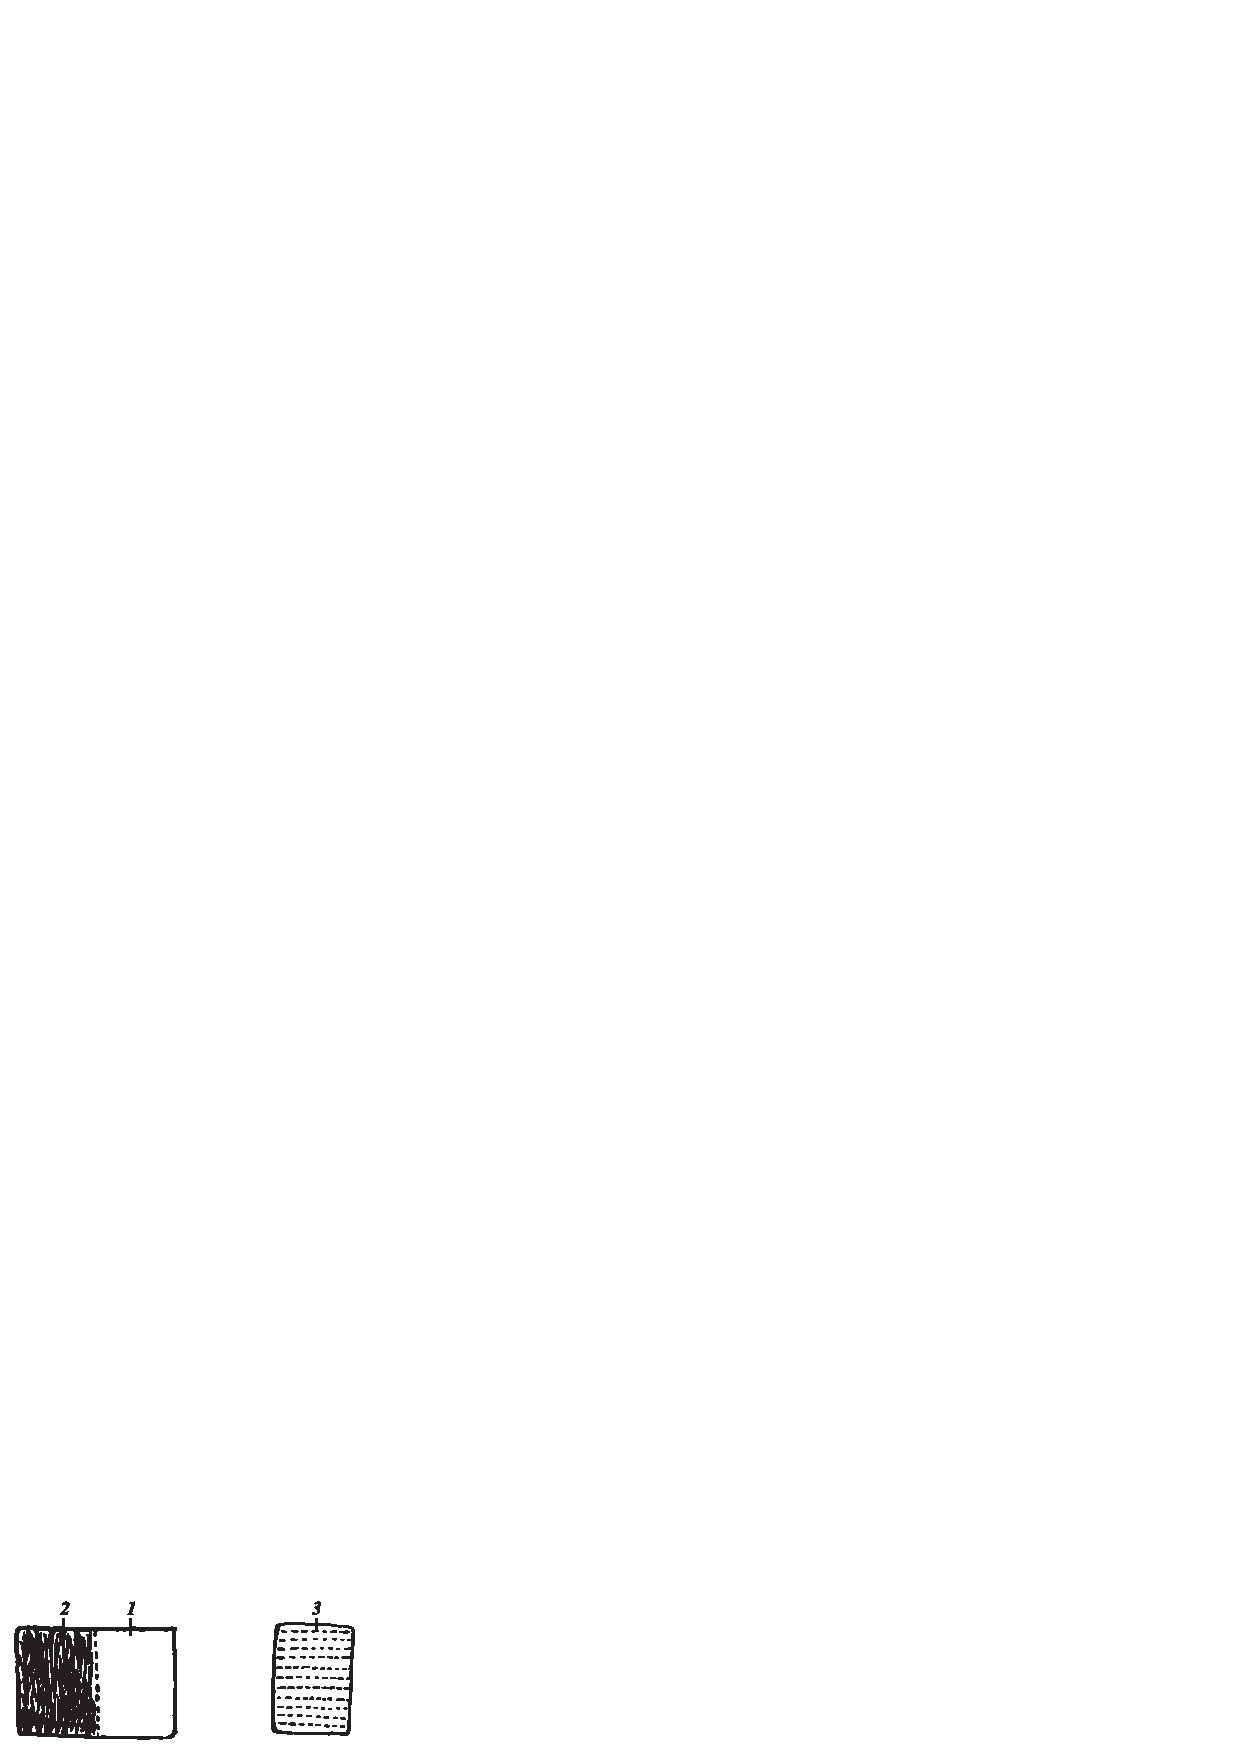
\includegraphics[scale=1]{illustration-003.pdf}%
\vspace{-.5625\baselineskip}%
\caption{松子肉包叠法图}%
\label{fig:wrapping}%
{\small 1.豆油皮\hspace{1em}2.肉丝\hspace{1em}3.叠好后}%
\end{wrapfigure}%
胡椒,于深碗中混合好,再与猪肉丝、萝卜丝、姜、葱一并拌匀。

\step 豆油皮一张修成六寸宽、八寸长,平铺案板上,而后把拌匀的猪肉丝、萝卜丝等铺
在豆油皮上,铺成七分厚,铺上豆油皮的一半,再把另一半叠过来,接头处涂蛋清豆粉封
口,如图\,\ref{fig:wrapping}\,。

\step 炒锅倒入菜油烧红,将叠好的豆油皮包放入炸透,炸成金黄色,滗去炸油,放盘中
晾冷。再用刀切成一寸半长、
\begin{wrapfigure}[5]{l}{10em}%
\centering%
\vspace{-1.25\baselineskip}%
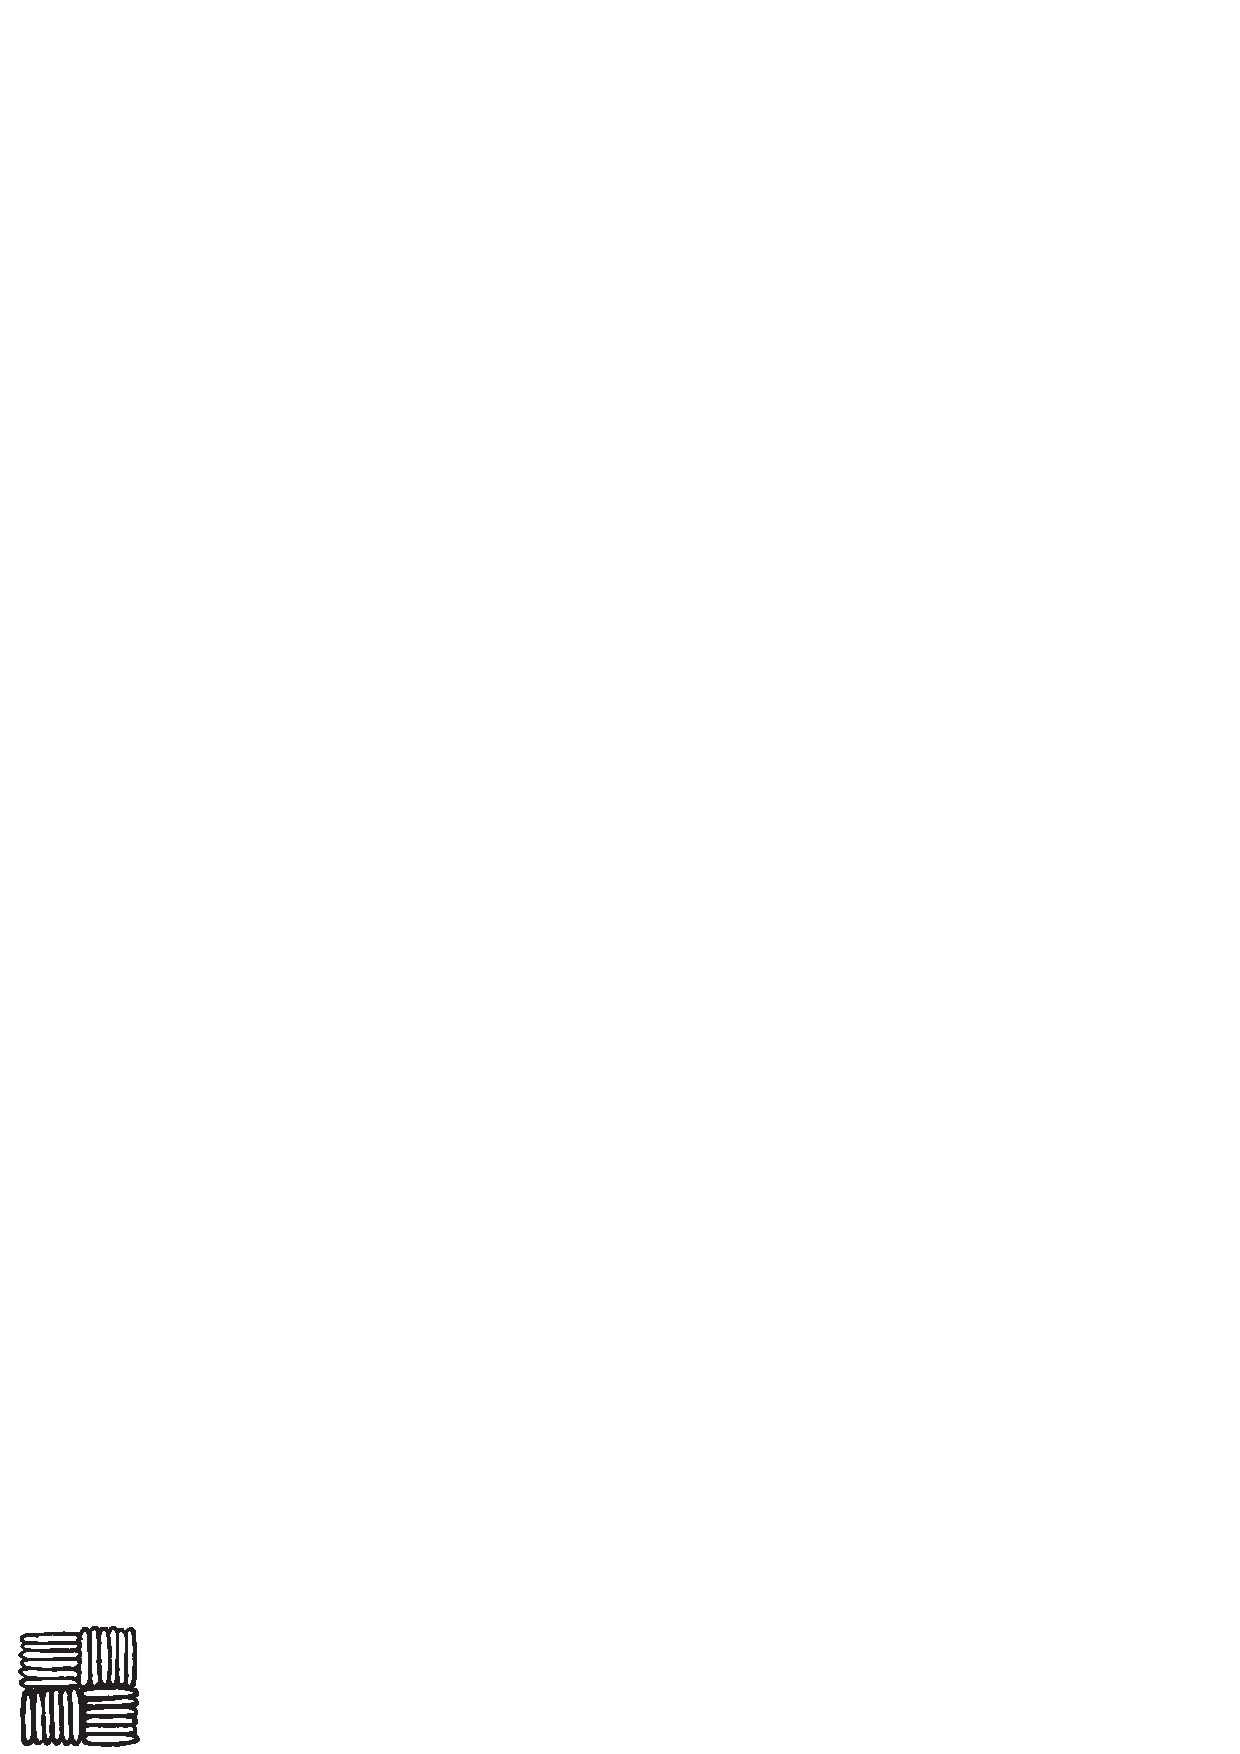
\includegraphics[scale=1]{illustration-004.pdf}%
\vspace{-.5625\baselineskip}%
\caption{松子肉摆法}%
\label{fig:presentation}%
\end{wrapfigure}%
三分宽、七分厚的长条,共二十四条。以六条为一组,于碗中镶成卍字形,如
图\,\ref{fig:presentation}\,。然后加二汤淹没肉条,上笼蒸三十分钟取出,扣于碗
内,再加奶汤四两、盐七分即成。

\features

此菜香软可口,营养丰富,特别适于冬季食用。

\end{recipe}

% vim: filetype=tex noautoindent nojoinspaces
% vim: fileencoding=utf-8 formatoptions+=m
% vim: textwidth=78 tabstop=4 shiftwidth=4 softtabstop=4

\begin{recipe}{晾干肉}

\ingredients

\ingredient{猪瘦肉}{一斤}
\ingredient{化猪油}{一两五}
\ingredient{大头菜}{一两}
\ingredient{酱油}{五钱}
\ingredient{姜}{二钱}
\ingredient{料酒}{五钱}
\ingredient{葱}{三钱}
\ingredient{胡椒面}{二分}

\ingredient{大蒜}{一个一}
\ingredient{味精,}{二分}
\ingredient{菜油}{半斤耗二两}
\ingredient{清汤}{三两}
\ingredient{香油}{二钱}
\ingredient{水豆粉}{三钱}
\ingredient{醋}{三钱}
\ingredient{白糖}{三钱}

\cooking

\step 大头菜削皮,横切成极薄的半圆形片葱、蒜去皮, 蒜切片,葱切马耳朵待用。

选猪后腿净瘦肉一斤,不拘规格,用平刀片成极薄的 肉片,贴于筲箕背,将肉铺开晾起,肉面洒上酱油、胡椒面、 料酒等,待两三小时后水气已晾干。

\step 	将菜油烧开,倒入干肉片炸黄,铲于墩子上,切成一 寸大小的姜糖块(即旗子块)。

\step 	化猪油二两入锅烧热,即投入葱、姜、蒜、醋、白糖、 清汤、香油,勾二流芡成汁,最后将炕酥的肉片、大头菜倒 入,一烹即成。

\notes

此菜在六十年前常用于碟子,为群众所喜爱,味甜酸, 肉香酥,颇有风味。

\end{recipe}

% vim: filetype=tex noautoindent
% vim: fileencoding=utf-8
% vim: textwidth=78 tabstop=4 shiftwidth=4 softtabstop=4

\begin{recipe}{麻圆肉}

\ingredients

\ingredient{猪保肋肉}{一斤}
\ingredient{千豆粉}{一两}
\ingredient{鸡蛋-}{二个}
\ingredient{面粉}{三钱}
\ingredient{白糖一}{四两}
\ingredient{茱油}{一斤半耗一两}
\ingredient{熟芝麻}{一两}

\cooking

\step 割去保肋痩肉,铲去肉皮,成猪肥膘。先在汤锅内煮透心(已熟)捞起,切成四分
见方的颗,再入沸水内汆一次,去其浮油,捞起晾干水气,即在连蛋黄的蛋豆粉内裹上一
层,即成待用的肉元。
\step 菜油烧至八成火,将肉元入油锅炸至浅黄色捞起。油泌尽后,在锅内放入白糖及少
许清水,炒至糖汁起大泡时加入芝麻,即倒入炸过的肉元,边炒边将锅几颠,使肉元裹糖
起锅。敞风,糖即干,盛盘。

\notes

以前多用于一般席桌的碟子上,以便客人包回家去。 味香甜,很象糖果店“麻圆果子”,
故名。

\end{recipe}

% vim: filetype=tex noautoindent
% vim: fileencoding=utf-8 formatoptions+=m
% vim: textwidth=78 tabstop=4 shiftwidth=4 softtabstop=4

\end{tocminipageleft}
\begin{tocminipageright}
\begin{recipe}{鹅黄肉}

\ingredients

\ingredient{肥痩肉}{半斤}
\ingredient{料酒}{五钱}
\ingredient{葱花}{二钱.}
\ingredient{鸡蛋}{五个}
\ingredient{胡椒面}{二分}
\ingredient{鱼辣椒}{五钱}
\ingredient{干豆粉}{一两}
\ingredient{菜油}{二斤耗二两}
\ingredient{醋}{五钱}
\ingredient{酱油}{三钱}
\ingredient{味精}{二分}
\ingredient{白糖}{三钱}
\ingredient{盐}{二钱}
\ingredient{姜米}{二钱}
\ingredient{郝:米}{二钱}

\cooking

\step 鸡蛋三个调勻,先在锅内摊成蛋皮二张。肥瘦肉剁成细末,加料酒、葱花、姜米、酱油、盐、味精、豆粉、胡椒面、鸡蛋一个,共拌匀成馅。

\step 蛋皮铺开全抹上蛋清豆粉,将拌好的馅裹成六条蛋卷,用手拍成宽六分、厚二分的扁形卷,用刀在卷的半面切成丝,半面不切(如切蜇卷样),然后再按一寸距离切为三十段。

\step 菜油烧至八成火,将切过的蛋卷入油锅内炸熟,捞起盛入盘内。

\step 锅内留适当的油,再放鱼香味作料,勾成二流芡滋汁,,淋上即成。

\notes

为肉制品中之多过程操作法,皮酥馅嫩,色鲜味浓,过 去常走于海参便饭行菜。

\end{recipe}

% vim: filetype=tex noautoindent
% vim: fileencoding=utf-8
% vim: textwidth=78 tabstop=4 shiftwidth=4 softtabstop=4

% BSD 3-Clause License
%
% Copyright (c) 2023 Quux System and Technology. All rights reserved.
%
% Redistribution and use in source and binary forms, with or without
% modification, are permitted provided that the following conditions are met:
%
% 1. Redistributions of source code must retain the above copyright notice, this
%    list of conditions and the following disclaimer.
%
% 2. Redistributions in binary form must reproduce the above copyright notice,
%    this list of conditions and the following disclaimer in the documentation
%    and/or other materials provided with the distribution.
%
% 3. Neither the name of the copyright holder nor the names of its
%    contributors may be used to endorse or promote products derived from
%    this software without specific prior written permission.
%
% THIS SOFTWARE IS PROVIDED BY THE COPYRIGHT HOLDERS AND CONTRIBUTORS "AS IS"
% AND ANY EXPRESS OR IMPLIED WARRANTIES, INCLUDING, BUT NOT LIMITED TO, THE
% IMPLIED WARRANTIES OF MERCHANTABILITY AND FITNESS FOR A PARTICULAR PURPOSE ARE
% DISCLAIMED. IN NO EVENT SHALL THE COPYRIGHT HOLDER OR CONTRIBUTORS BE LIABLE
% FOR ANY DIRECT, INDIRECT, INCIDENTAL, SPECIAL, EXEMPLARY, OR CONSEQUENTIAL
% DAMAGES (INCLUDING, BUT NOT LIMITED TO, PROCUREMENT OF SUBSTITUTE GOODS OR
% SERVICES; LOSS OF USE, DATA, OR PROFITS; OR BUSINESS INTERRUPTION) HOWEVER
% CAUSED AND ON ANY THEORY OF LIABILITY, WHETHER IN CONTRACT, STRICT LIABILITY,
% OR TORT (INCLUDING NEGLIGENCE OR OTHERWISE) ARISING IN ANY WAY OUT OF THE USE
% OF THIS SOFTWARE, EVEN IF ADVISED OF THE POSSIBILITY OF SUCH DAMAGE.
%
\begin{recipe}{松花肉}

\ingredients

\ingredient{猪肥瘦肉}{二两五}
\ingredient{五香面}{一分}
\ingredient{水发口蘑}{三钱}
\ingredient{鸡蛋}{六个}
\ingredient{味精}{三分}
\ingredient{葱花}{三钱}
\ingredient{酱油}{三钱}
\ingredient{料酒}{二钱}
\ingredient{面粉}{一两}
\ingredient{白糖}{一分}
\ingredient{化猪油}{一斤二两耗二两五}
\ingredient{盐}{二分}
\ingredient{豆尖}{数根}

\preparation

\step 蛋黄调散,蛋清快速调成蛋泡。面粉过箩筛,同味精、盐慢慢加入蛋泡内,用筷子
轻轻调匀待用。

\step 猪肉、冬笋、口蘑,分别用刀剁碎。锅内放猪油少许,将猪肉调匀,依次加入蛋
黄、冬笋、口蘑、料酒及葱花、酱油、白糖、五香面等,炒熟成焰子,起锅待用。

\step 炒锅置于文火上,将猪油烧至三成热,把调好的蛋泡倒入一半,煎成圆形、直径约
六寸的蛋饼。将炒熟的馅子,倒于蛋饼中心,立即将另一半蛋泡盖于馅子上,并按上鲜豆
尖。同时另用一锅将全部猪油烧沸,再慢慢舀淋入锅内的蛋泡上。油舀完约五分钟,滗去
油,扦入盘内即成。

\features

泡嫩,鲜香,美观适口。

\end{recipe}

% vim: filetype=tex noautoindent nojoinspaces
% vim: fileencoding=utf-8 formatoptions+=m
% vim: textwidth=78 tabstop=4 shiftwidth=4 softtabstop=4

\begin{recipe}{南卤肉}

\ingredients

\ingredient{猪肉}{一斤半}
\ingredient{盐}{五分}
\ingredient{白糖}{三钱}
\ingredient{南豆腐乳水}{二两}
\ingredient{葱}{五钱}
\ingredient{姜}{一钱}

\preparation

\step 选五花肉,切成长一寸五、厚三分的骨牌片。葱切成两寸长的节。姜洗净,刮皮,
拍破,对剖。
\step 油在锅内烧至七成热。将肉熵干水气,加入盐、白糖、料酒、葱、姜,然后烹入清
水。在旺火上烧开后,打净泡沫,加豆腐乳汁,移至文火上锆至肉粑,拈去姜渣,盛入白
瓷条盘。

\features

粑嫩香美,酒饭均宜。

\end{recipe}

% vim: filetype=tex noautoindent nojoinspaces
% vim: fileencoding=utf-8 formatoptions+=m
% vim: textwidth=78 tabstop=4 shiftwidth=4 softtabstop=4

\begin{recipe}[金银肉糕]{双色肉糕}

\ingredients

\ingredient{猪肥瘦肉}{一斤}
\ingredient{鸡蛋清}{六个}
\ingredient{干豆粉}{一两五}
\ingredient{花概面}{一分}
\ingredient{姜}{三钱}
\ingredient{葱}{三钱}
\ingredient{盐}{五分}
\ingredient{料酒}{三钱}
\ingredient{清汤}{六两}
\ingredient{化猪油}{二两}
\ingredient{味精}{三分}

\preparation

\step .猪肉剁成肉茸;鸡蛋破壳,蛋清、蛋黄分开搅散(不起泡);葱、姜切成细末。
\step :肉茸加蛋清、盐、花椒面、姜、葱、豆粉、味精,拌匀成馅。
\step 平底瓷盘,盘底抹油,四方框上木板高一寸,过心四寸。先倒入蛋清,上笼蒸三分
钟至熟。即将拌好的馅倒在蛋清上面,用手抹平,倒上蛋黄抹平再上笼蒸透。取出启去底
板晾冷,切成大骨牌片,长一寸二。用二鱼碗定成三叠水或风车式,加汤一两,再上笼蒸
透,取出翻入盘内。
\step 锅内的油烧热掺汤下锅,加盐、味精、料酒,勾芡扯成白汁,淋上肉糕即成。

\features

鲜嫩美观,适合老年人食用。

\end{recipe}

% vim: filetype=tex noautoindent nojoinspaces
% vim: fileencoding=utf-8 formatoptions+=m
% vim: textwidth=78 tabstop=4 shiftwidth=4 softtabstop=4

\begin{recipe}{芙蓉肉糕}

\ingredients

\ingredient{肥瞟肉}{五两}
\ingredient{红糖}{三两}
\ingredient{白糖}{二两}
\ingredient{鸡蛋}{二个}
\ingredient{菜油}{一斤半耗二两}
\ingredient{红色素}{少许}
\ingredient{干豆粉}{二两}
\ingredient{青糖}{少许}

\cooking

\step 	肥膘肉煮熟,切成长一寸五的二祖丝,下沸水锅汆过 (去油〉,用漏瓢滤起,在盘内晾干水气,再将蛋清豆粉与

肉丝调拌均匀。

\step 	将肉丝用手拌散,撒入七成火候的油锅,随即用漏瓢 打起。撕散,再入八成火候的油锅,炸脆,起锅待用。

\step 	将红糖熬起泡时加青糖,将肉丝倒入。随手将锅提起 来造转,再倒进搪瓷方盘。用铲或刀按平约七分厚,面上撒 一层胭脂糖(白糖用色素调成〉。晾冷后切成姜糖块(即斜 方块〉,装入条盘。

\notes

此菜约六、七十年的历史,可上热食,亦可上冷盘,又 可上海参席,脆甜可口,解酒佳肴。	「‘

\end{recipe}

% vim: filetype=tex noautoindent
% vim: fileencoding=utf-8
% vim: textwidth=78 tabstop=4 shiftwidth=4 softtabstop=4

\vspace{1\baselineskip}
\begin{recipe}{焦皮肘子}

\ingredients

\ingredient{净肘子}{一个(约二斤半)}
\ingredient{化猪油}{二两}
\ingredient{冰糖}{二两}
\ingredient{料酒}{二两}
\ingredient{酱油}{二两}
\ingredient{姜}{五饯}
\ingredient{葱}{五钱}
\ingredient{盐}{三分}
\ingredient{水豆粉}{二钱}
\ingredient{清场}{三斤}
\ingredient{碎骨}{一斤}

\preparation

\step 将肘子残毛抬去,放在炭火上烧,至皮呈焦黑时,丢入热水内泡半点钟,至皮已软
后,取出,用刀全部刮去烧黑的一层,现出黄色时,入清水清洗两次待用。

\step 鼎锅置于旺火上,放入碎骨垫底,加汤,再投人肘子。汤一冲开,打净血泡,即端
离旺火放在小火上焙起。

\step 油在炒锅内用庇火烧热,下冰糖炒成汁,舀入少许鼎 锅内的汤把糖汁冲散。加料
酒、酱油、葱(挽成结》、姜(拍 破:)、盐,用汤瓢荡匀翻入鼎锅。继续焙两小时,用
筷子将 肘子拈入大元盘摆好。滋汁泌入炒锅内,加味精,勾芡,收 酽后淋在肘子上即成。

\features

颜色红亮,味浓香美,肥而不腻。

\end{recipe}

% vim: filetype=tex noautoindent
% vim: fileencoding=utf-8 formatoptions+=m
% vim: textwidth=78 tabstop=4 shiftwidth=4 softtabstop=4

% BSD 3-Clause License
%
% Copyright (c) 2023 Quux System and Technology. All rights reserved.
%
% Redistribution and use in source and binary forms, with or without
% modification, are permitted provided that the following conditions are met:
%
% 1. Redistributions of source code must retain the above copyright notice, this
%    list of conditions and the following disclaimer.
%
% 2. Redistributions in binary form must reproduce the above copyright notice,
%    this list of conditions and the following disclaimer in the documentation
%    and/or other materials provided with the distribution.
%
% 3. Neither the name of the copyright holder nor the names of its
%    contributors may be used to endorse or promote products derived from
%    this software without specific prior written permission.
%
% THIS SOFTWARE IS PROVIDED BY THE COPYRIGHT HOLDERS AND CONTRIBUTORS "AS IS"
% AND ANY EXPRESS OR IMPLIED WARRANTIES, INCLUDING, BUT NOT LIMITED TO, THE
% IMPLIED WARRANTIES OF MERCHANTABILITY AND FITNESS FOR A PARTICULAR PURPOSE ARE
% DISCLAIMED. IN NO EVENT SHALL THE COPYRIGHT HOLDER OR CONTRIBUTORS BE LIABLE
% FOR ANY DIRECT, INDIRECT, INCIDENTAL, SPECIAL, EXEMPLARY, OR CONSEQUENTIAL
% DAMAGES (INCLUDING, BUT NOT LIMITED TO, PROCUREMENT OF SUBSTITUTE GOODS OR
% SERVICES; LOSS OF USE, DATA, OR PROFITS; OR BUSINESS INTERRUPTION) HOWEVER
% CAUSED AND ON ANY THEORY OF LIABILITY, WHETHER IN CONTRACT, STRICT LIABILITY,
% OR TORT (INCLUDING NEGLIGENCE OR OTHERWISE) ARISING IN ANY WAY OUT OF THE USE
% OF THIS SOFTWARE, EVEN IF ADVISED OF THE POSSIBILITY OF SUCH DAMAGE.
%
\begin{recipe}{烧皱皮肉}

\ingredients

\ingredient{五花猪肉}{一方二斤}
\ingredient{冰糖}{一两}
\ingredient{姜}{三钱}
\ingredient{葱}{三钱}
\ingredient{料酒}{二钱}
\ingredient{咸红酱油}{三钱}
\ingredient{盐}{一钱二}
\ingredient{香料}{二钱}
\ingredient{清汤}{一斤半}
\ingredient{菜油}{一斤耗一两}
\ingredient{鸡足(或鸡骨、猪肋骨均可)}{酌量}

\preparation

\step 将猪肉残毛拈去,刮洗干净。入汤锅,除尽血水。煮熟捞起,用净布搌干水气,
抹上酱油后投入烧至八成热的油锅内,炸至皮色金黄起皱时捞起。葱切成长节,姜拍破待
用。

\step 用铝锅一个,把洗净的鸡(或骨)放入垫底,取其鲜味,且避免巴锅,上面铺放炸
好的猪肉,必须猪皮向上。随即用炒锅炒好冰糖汁,烹入清汤并加料酒、盐、香料、葱、
姜,浪转后倒入铝锅。在微火上烧至六成𤆵时,将猪肉翻面,肉皮即向下了,继续以微火
烧𤆵。此时汤已收酽,把滋汁滗入碗内,即将肉翻入圆盘,拣去垫底的骨头及姜、葱,然
后淋上滋汁即成。

\features

味鲜带甜,𤆵香可口,宜于老年人食用。

\end{recipe}

% vim: filetype=tex noautoindent nojoinspaces
% vim: fileencoding=utf-8 formatoptions+=m
% vim: textwidth=78 tabstop=4 shiftwidth=4 softtabstop=4

\begin{recipe}{芝麻肘子}

\ingredients

\ingredient{肘子}{二斤}
\ingredient{芝麻}{二两}
\ingredient{冰糖}{二两}
\ingredient{盐}{五分}
\ingredient{料酒}{一两}
\ingredient{姜、葱}{各五钱}
\ingredient{白糖}{二两}
\ingredient{清汤}{三斤}

\ingredient{桃红食色}{少泮}

\cooking

\step 肘子在炉火上将粗皮一层烧成焦色的皱纹状时,泡在 温水内刮洗干净,在沸水内除去焦味,检去泡沫。用锑锅一 个,先在内面垫上一层猪骨或鸡、鸭骨,再将肘子放在骨上 (:皮朝下〉,掺入全部清汤、料酒、姜、葱、盐及三分之一 的冰糖炒的糖汁。在中火上烧至五成钯时,再投入余下的冰

糖,继续烧至全炤为止。

\step 芝麻淘洗后,去壳炒熟,用杆仗碾一下。白糖、食色 兑成胭脂糖,连芝麻造匀。走菜时先将烧炤的肘子拈入盘中 放好,将原汁烧浓淋上面,即将造合过的芝麻撒在肘子上即 成。

\notes

味甜咸,颜色深浓,有芝麻香味。

\end{recipe}

% vim: filetype=tex noautoindent
% vim: fileencoding=utf-8
% vim: textwidth=78 tabstop=4 shiftwidth=4 softtabstop=4

% BSD 3-Clause License
%
% Copyright (c) 2023 Quux System and Technology. All rights reserved.
%
% Redistribution and use in source and binary forms, with or without
% modification, are permitted provided that the following conditions are met:
%
% 1. Redistributions of source code must retain the above copyright notice, this
%    list of conditions and the following disclaimer.
%
% 2. Redistributions in binary form must reproduce the above copyright notice,
%    this list of conditions and the following disclaimer in the documentation
%    and/or other materials provided with the distribution.
%
% 3. Neither the name of the copyright holder nor the names of its
%    contributors may be used to endorse or promote products derived from
%    this software without specific prior written permission.
%
% THIS SOFTWARE IS PROVIDED BY THE COPYRIGHT HOLDERS AND CONTRIBUTORS "AS IS"
% AND ANY EXPRESS OR IMPLIED WARRANTIES, INCLUDING, BUT NOT LIMITED TO, THE
% IMPLIED WARRANTIES OF MERCHANTABILITY AND FITNESS FOR A PARTICULAR PURPOSE ARE
% DISCLAIMED. IN NO EVENT SHALL THE COPYRIGHT HOLDER OR CONTRIBUTORS BE LIABLE
% FOR ANY DIRECT, INDIRECT, INCIDENTAL, SPECIAL, EXEMPLARY, OR CONSEQUENTIAL
% DAMAGES (INCLUDING, BUT NOT LIMITED TO, PROCUREMENT OF SUBSTITUTE GOODS OR
% SERVICES; LOSS OF USE, DATA, OR PROFITS; OR BUSINESS INTERRUPTION) HOWEVER
% CAUSED AND ON ANY THEORY OF LIABILITY, WHETHER IN CONTRACT, STRICT LIABILITY,
% OR TORT (INCLUDING NEGLIGENCE OR OTHERWISE) ARISING IN ANY WAY OUT OF THE USE
% OF THIS SOFTWARE, EVEN IF ADVISED OF THE POSSIBILITY OF SUCH DAMAGE.
%
\begin{recipe}[东坡肉]{罐烧肉}

\ingredients

\ingredient{肥五花猪肉}{一方约二斤}
\ingredient{冰糖}{一两}
\ingredient{姜}{一钱}
\ingredient{葱白}{一两}
\ingredient{花椒}{约十颗}
\ingredient{菜油}{八两}
\ingredient{鸡骨头}{酌量}
\ingredient{盐}{一钱}
\ingredient{酱油}{三钱}
\ingredient{二汤}{二斤半}
\ingredient{料酒}{四两}

\preparation

\step 猪肉拈尽残毛,刮洗干净,入沸水锅内煮十分钟,除去血水,捞起晾干水气。冰糖
炒成金黄色的糖汁。

\step 油在锅内烧红,将猪肉放入,使猪皮向下,不断用汤瓢舀炸油浇淋,炸成淡黄色捞
起。

\step 取用包罐(或铝锅),垫上鸡骨(鸡足、翅、篾巴均可),将肉皮向上放入包罐,
加酱油、葱、姜、料酒、花椒、盐、糖汁、冰糖,二汤淹过猪肉两寸,在武火上烧沸后改
用文火烧至七成𤆵时,将猪肉翻面继续烧𤆵盛入盘内,再将收浓的滋汁滗起淋上即成。

\features

菜色红亮,肥美鲜香。

\end{recipe}

% vim: filetype=tex noautoindent nojoinspaces
% vim: fileencoding=utf-8 formatoptions+=m
% vim: textwidth=78 tabstop=4 shiftwidth=4 softtabstop=4

% BSD 3-Clause License
%
% Copyright (c) 2023 Quux System and Technology. All rights reserved.
%
% Redistribution and use in source and binary forms, with or without
% modification, are permitted provided that the following conditions are met:
%
% 1. Redistributions of source code must retain the above copyright notice, this
%    list of conditions and the following disclaimer.
%
% 2. Redistributions in binary form must reproduce the above copyright notice,
%    this list of conditions and the following disclaimer in the documentation
%    and/or other materials provided with the distribution.
%
% 3. Neither the name of the copyright holder nor the names of its
%    contributors may be used to endorse or promote products derived from
%    this software without specific prior written permission.
%
% THIS SOFTWARE IS PROVIDED BY THE COPYRIGHT HOLDERS AND CONTRIBUTORS "AS IS"
% AND ANY EXPRESS OR IMPLIED WARRANTIES, INCLUDING, BUT NOT LIMITED TO, THE
% IMPLIED WARRANTIES OF MERCHANTABILITY AND FITNESS FOR A PARTICULAR PURPOSE ARE
% DISCLAIMED. IN NO EVENT SHALL THE COPYRIGHT HOLDER OR CONTRIBUTORS BE LIABLE
% FOR ANY DIRECT, INDIRECT, INCIDENTAL, SPECIAL, EXEMPLARY, OR CONSEQUENTIAL
% DAMAGES (INCLUDING, BUT NOT LIMITED TO, PROCUREMENT OF SUBSTITUTE GOODS OR
% SERVICES; LOSS OF USE, DATA, OR PROFITS; OR BUSINESS INTERRUPTION) HOWEVER
% CAUSED AND ON ANY THEORY OF LIABILITY, WHETHER IN CONTRACT, STRICT LIABILITY,
% OR TORT (INCLUDING NEGLIGENCE OR OTHERWISE) ARISING IN ANY WAY OUT OF THE USE
% OF THIS SOFTWARE, EVEN IF ADVISED OF THE POSSIBILITY OF SUCH DAMAGE.
%
\begin{recipe}{红枣煨肘}

\ingredients

\ingredient{猪肘}{二斤}
\ingredient{红枣}{二两}
\ingredient{冰糖}{六两}

\preparation

\step 猪肘拈尽毛桩,刮洗干净,在煮锅内除去血腥味。红枣洗干净。

\step 小铝锅一个,先在底上垫几块细瓷瓦片,掺水二斤,将肘子放入,在旺火上烧开,
打去泡沫。将冰糖炒成深黄色糖汁倒下,连同其余冰糖、红枣在锅内烧一小时,再移文火
上慢煨二小时。待肘子煨至𤆵、烂、粘稠,汁酽即起锅。

\features

𤆵烂、甜香,入口粘稠,富于营养,老年人最为适宜。

\end{recipe}

% vim: filetype=tex noautoindent nojoinspaces
% vim: fileencoding=utf-8 formatoptions+=m
% vim: textwidth=78 tabstop=4 shiftwidth=4 softtabstop=4

\begin{recipe}{南照兀子}

\ingredients

\ingredient{猪肉}{肥半斤瘦一斤(去骨皮)}
\ingredient{熟火腿}{一两}
\ingredient{水发兰片}{一两}
\ingredient{水发香菌}{一两}
\ingredient{鸡蛋}{二个}
\ingredient{慈姑}{六个}
\ingredient{菜心}{五两}
\ingredient{菜油}{一斤}
\ingredient{酱油}{五钱}
\ingredient{姜}{五钱}
\ingredient{葱白}{五钱}
\ingredient{水豆粉}{一'两五}
\ingredient{香油}{二钱}
\ingredient{盐}{五分}
\ingredient{料酒}{五分}
\ingredient{胡椒、妹精}{各少许}

\cooking

\step 菜心淘净,沮好;慈菇削皮;香菌洗净泥沙。
\step 猪肉切成小豌豆大的丁,火腿、兰片、香菌、慈菇,分别切成细丁;葱切细花;姜
去皮切细末。以上各材料加盐、酱油、水豆粉、鸡蛋(连黄)搅匀,共作成四个肉元子略
按扁。
\step 油烧至七成热,肉元煎成金黄色,捞起入碗,加姜、葱,搭汤上笼,蒸炤。
\step 走菜时将元子拈在盘内摆好,菜心用原汁加料酒、胡椒、盐、味精、酱油,吃味后
镶在菜的周围,余汁用水豆粉扯成滋汁,加香油淋上即成。

\notes

颜色金黄,质地细软,鲜香可口上大元盘。

\end{recipe}

% vim: filetype=tex noautoindent
% vim: fileencoding=utf-8
% vim: textwidth=78 tabstop=4 shiftwidth=4 softtabstop=4

\begin{recipe}{苕菜狮子头}

\ingredients

\ingredient{冬干苕菜}{二两}
\ingredient{肥瘦肉}{各半斤}
\ingredient{慈菇}{三两}
\ingredient{金钩}{五钱}
\ingredient{肥火腿}{一两}
\ingredient{鲜青豆}{二两}
\ingredient{鸡蛋}{二个}
\ingredient{干豆粉}{一两}
\ingredient{鸡油}{一两}
\ingredient{化猪油}{一斤耗三两}
\ingredient{料酒}{五钱}
\ingredient{盐}{六分}
\ingredient{胡椒}{一分}
\ingredient{味精}{三分}
\ingredient{姜、葱}{各三钱}
\ingredient{清汤}{二斤}

\preparation

\step 金钩用清水发胀,慈菇去皮,肥痩肉、火腿、鲜青豆等分别切成碎颗,鸡蛋清与豆
粉调成蛋清豆粉,同时盛入碗内,再放入盐、料酒、胡椒、味精等,用手拌匀,按四分之
一捏成四个扁形的丸子,放入锅内(锅内有猪油),炸进皮肘,不见黄色即捞起。

\step 用小包罐一个洗净,将捞起的丸子放下,加入清汤、姜、葱及剩余全部作料,放在
文火上烧二时。烧至半熟时将淘洗干净的苕菜放入,继续烧至熟透为止。走菜时用深圆盘
先将四个丸子摆成四方形,将苕菜镶于四周围,将罐内的原汁灌入呈半汤形,淋入鸡油即
成。

\features

味道鲜美,清香。

\end{recipe}

% vim: filetype=tex noautoindent nojoinspaces
% vim: fileencoding=utf-8 formatoptions+=m
% vim: textwidth=78 tabstop=4 shiftwidth=4 softtabstop=4

\begin{recipe}{软炸蒸肉}

\ingredients

\ingredient{猪肥膘一方}{一斤}
\ingredient{鲜豌豆(或黄豆)}{四两}
\ingredient{五香粉}{半分}
\ingredient{面包}{一个}
\ingredient{花椒面}{一分}
\ingredient{耢糟}{五钱}
\ingredient{酱油}{五钱}
\ingredient{豆腐乳水}{五钱}
\ingredient{姜米}{一钱}
\ingredient{白糖}{五钱}
\ingredient{葱花}{五钱}
\ingredient{菜油}{一斤半耗一两五}
\ingredient{鸡蛋}{二个}
\ingredient{料酒}{一两}
\ingredient{甜酱}{五钱}
\ingredient{盐}{二分}
\ingredient{大米粉}{二两}

\cooking

\step 猪肉刮洗干净,切成两寸长、一分半厚的片,装在大碗内。将花椒、五香粉、酱
油、豆腐乳水、耢糟、白糖、姜米、葱花、盐、料酒在碗内兑好调匀。豌豆洗净。面包揉
成细粉。鸡蛋打破搅勻。盐、花椒合成椒盐。
\step 将兑好的调料倒在肉片碗内造匀,码二十分钟,再加米粉、豌豆,拌匀后,将肉片
摆入洗净的二鱼碗底成一封书形,面上装豌豆,上笼蒸粑,取出翻在另外的二鱼碗,拈出
肉片晾冷,豌豆仍上笼馏起。
\step 晾冷的蒸肉两面抹上搅好的鸡蛋,再挨个地两面沾满面包粉,下入八成热的油锅
内,炸呈余黄色捞起,装在条盘中心。
\step 将豌豆取出,装在蒸肉条盘的一端,另端镶椒盐及白糖两味即成。

\notes

香酥味鲜,可甜可咸,别具风味。

\end{recipe}

% vim: filetype=tex noautoindent
% vim: fileencoding=utf-8
% vim: textwidth=78 tabstop=4 shiftwidth=4 softtabstop=4

\begin{recipe}{软炸子盖}

\ingredients

\ingredient{猪肉一方}{一斤半}
\ingredient{菜油}{一斤半耗二两}
\ingredient{咸“酱油}{二钱五}
\ingredient{酱油}{一钱二}
\ingredient{料酒}{一钱二}
\ingredient{鸡蛋清}{三个}
\ingredient{干豆粉}{一两二}
\ingredient{葱白}{三两}
\ingredient{鉗酱}{四钱}
\ingredient{蒜}{一'两}
\ingredient{香油}{三分}
\ingredient{姜}{二汽}

\cooking

\step 选五花猪肉一方,放入汤锅内煮三分钟,去净血水泡 沫,捞出晾冷,去皮,切二分厚的片,盛入大碗中,加料酒, 红、白酱油,再把老姜拍松,葱切段拌匀,平放于大平盘中, 上笼蒸一点半钟,出笼泌去汁水,晾冷待用。

\step 鸡蛋清和干豆粉一起拌匀。甜酱和香油一起拌匀。蒜 切成片。葱白洗净,切成一寸长的段。

\step 锅放炉上烧红,将菜油放入烧至七成热,用净布一方 在开水中浸湿,拧干水后,将五花肉片上的油擦干净。用竹 筷将肉片一片片地夹起,裹满蛋清豆粉,放入油锅内炸。炸 至黄色、酥皮时起锅,淋香油,然后用刀切成斜方块,摆入 条盘的一端。另一端摆蒜片、甜酱、葱白段入席。

\notes

此菜外酥内粑,颜色金黄。

\end{recipe}

% vim: filetype=tex noautoindent
% vim: fileencoding=utf-8
% vim: textwidth=78 tabstop=4 shiftwidth=4 softtabstop=4

% BSD 3-Clause License
%
% Copyright (c) 2023 Quux System and Technology. All rights reserved.
%
% Redistribution and use in source and binary forms, with or without
% modification, are permitted provided that the following conditions are met:
%
% 1. Redistributions of source code must retain the above copyright notice, this
%    list of conditions and the following disclaimer.
%
% 2. Redistributions in binary form must reproduce the above copyright notice,
%    this list of conditions and the following disclaimer in the documentation
%    and/or other materials provided with the distribution.
%
% 3. Neither the name of the copyright holder nor the names of its
%    contributors may be used to endorse or promote products derived from
%    this software without specific prior written permission.
%
% THIS SOFTWARE IS PROVIDED BY THE COPYRIGHT HOLDERS AND CONTRIBUTORS "AS IS"
% AND ANY EXPRESS OR IMPLIED WARRANTIES, INCLUDING, BUT NOT LIMITED TO, THE
% IMPLIED WARRANTIES OF MERCHANTABILITY AND FITNESS FOR A PARTICULAR PURPOSE ARE
% DISCLAIMED. IN NO EVENT SHALL THE COPYRIGHT HOLDER OR CONTRIBUTORS BE LIABLE
% FOR ANY DIRECT, INDIRECT, INCIDENTAL, SPECIAL, EXEMPLARY, OR CONSEQUENTIAL
% DAMAGES (INCLUDING, BUT NOT LIMITED TO, PROCUREMENT OF SUBSTITUTE GOODS OR
% SERVICES; LOSS OF USE, DATA, OR PROFITS; OR BUSINESS INTERRUPTION) HOWEVER
% CAUSED AND ON ANY THEORY OF LIABILITY, WHETHER IN CONTRACT, STRICT LIABILITY,
% OR TORT (INCLUDING NEGLIGENCE OR OTHERWISE) ARISING IN ANY WAY OUT OF THE USE
% OF THIS SOFTWARE, EVEN IF ADVISED OF THE POSSIBILITY OF SUCH DAMAGE.
%
\begin{recipe}{炸班指}

\ingredients

\ingredient{猪肥肠头}{三段(约二斤)}
\ingredient{葱白}{一两}
\ingredient{鸡蛋黄}{一个}
\ingredient{盐}{七钱}
\ingredient{生菜}{二两}
\ingredient{酱油}{三钱}
\ingredient{白糖}{四钱}
\ingredient{清汤}{二两}
\ingredient{甜酱}{三钱}
\ingredient{醋}{四钱}
\ingredient{白矾(研细)}{二钱}
\ingredient{菜油}{一斤半耗一两}
\ingredient{姜(去皮)}{三钱五}
\ingredient{花椒}{十余粒}
\ingredient{料酒}{七钱}
\ingredient{水豆粉}{二钱五}
\ingredient{咖喱}{一分}
\ingredient{蒜}{四钱}
\ingredient{香油}{四钱}

\preparation

\step 选用体厚质佳的肥肠头三段,靠近肛门部份切去一圈不用,在清水中加入白矾末,
把肥肠放入,用力揉搓清洗一次,除去粘液涎水;另换清水加盐,同样揉搓清洗两次。即
把肠的里面(有油的一面)翻出来,用刀撕去油上粘的杂质脏物(注意不要撕掉油),再
继续用水清洗。这样两面反复多洗几次,直到肥肠白净涩手,无臭味为止。最后仍把有油
的一面翻到内面去,洗净后放在开水锅内煮一刻钟捞出。再把肠两端用刀修去一分左右,
使之整齐。每段再分别切成两段(共六段)。用大蒸碗盛起,放入清水、盐、葱白三段、
料酒、花椒、姜等佐料,使水淹没过肥肠,上笼用旺火蒸三小时,至肥肠起着皱折为适
合。

\step 葱白用刀切成一寸长段,两头切成细花翻起。甜酱用香油、白糖拌合调匀。大蒜去
皮,切成四分见方、半分厚的片。生菜洗净,用香油、醋少许、蛋黄、白糖、咖喱拌合
(炸班指时才拌)。葱、姜、大蒜分别用刀切成细末,和香油、料酒、清汤、水豆粉、白
糖、醋、酱油等佐料,用碗盛好调匀,成为糖醋汁。

\step 菜油倒入炒锅内烧沸,将蒸好的肥肠取出(要炸时才取,葱、姜等不要),放在盘
内将水滗干,顺着锅边放入锅内,并立即用汤瓢将肠拨横过来,不使两头肠口向着人(因
为肠内有水,刚一下锅要炸几下,溅起来的油容易烫伤人)。炸时要用汤瓢拨动肥肠,以
便炸匀。约五分钟,肠呈金红色,即把油滗去,淋上香油,颠两下即捞出。然后在案板上
用刀把肥肠切成四分厚的圆圈,堆在盘的中间,盘的两端分别放上拌好的生菜和葱酱蒜。
再在炸班指的原锅内将糖醋汁煎热,盛在两个汤杯内,与班指一同上桌。

\features

此菜色泽金红,皮酥里嫩,细软而香,吃时可佐以葱酱蒜,也可以蘸糖醋汁,还可以伴生
菜叶,都各有风味。因肥肠成圆形,似射箭的班指一样,故名。

\end{recipe}

% vim: filetype=tex noautoindent nojoinspaces
% vim: fileencoding=utf-8 formatoptions+=m
% vim: textwidth=78 tabstop=4 shiftwidth=4 softtabstop=4

% BSD 3-Clause License
%
% Copyright (c) 2023 Quux System and Technology. All rights reserved.
%
% Redistribution and use in source and binary forms, with or without
% modification, are permitted provided that the following conditions are met:
%
% 1. Redistributions of source code must retain the above copyright notice, this
%    list of conditions and the following disclaimer.
%
% 2. Redistributions in binary form must reproduce the above copyright notice,
%    this list of conditions and the following disclaimer in the documentation
%    and/or other materials provided with the distribution.
%
% 3. Neither the name of the copyright holder nor the names of its
%    contributors may be used to endorse or promote products derived from
%    this software without specific prior written permission.
%
% THIS SOFTWARE IS PROVIDED BY THE COPYRIGHT HOLDERS AND CONTRIBUTORS "AS IS"
% AND ANY EXPRESS OR IMPLIED WARRANTIES, INCLUDING, BUT NOT LIMITED TO, THE
% IMPLIED WARRANTIES OF MERCHANTABILITY AND FITNESS FOR A PARTICULAR PURPOSE ARE
% DISCLAIMED. IN NO EVENT SHALL THE COPYRIGHT HOLDER OR CONTRIBUTORS BE LIABLE
% FOR ANY DIRECT, INDIRECT, INCIDENTAL, SPECIAL, EXEMPLARY, OR CONSEQUENTIAL
% DAMAGES (INCLUDING, BUT NOT LIMITED TO, PROCUREMENT OF SUBSTITUTE GOODS OR
% SERVICES; LOSS OF USE, DATA, OR PROFITS; OR BUSINESS INTERRUPTION) HOWEVER
% CAUSED AND ON ANY THEORY OF LIABILITY, WHETHER IN CONTRACT, STRICT LIABILITY,
% OR TORT (INCLUDING NEGLIGENCE OR OTHERWISE) ARISING IN ANY WAY OUT OF THE USE
% OF THIS SOFTWARE, EVEN IF ADVISED OF THE POSSIBILITY OF SUCH DAMAGE.
%
\begin{recipe}{软炸肚头}

\ingredients

\ingredient{猪肚头}{四两}
\ingredient{干豆粉}{五钱}
\ingredient{料酒}{一钱}
\ingredient{葱}{二钱}
\ingredient{盐}{五分}
\ingredient{鸡蛋清}{一个半}
\ingredient{猪油}{一斤耗一两五}
\ingredient{姜}{一钱}
\ingredient{香油}{五分}
\ingredient{花椒末}{五分}
\ingredient{醋}{五钱}

\preparation

\step 猪肚头洗净去筋,切成一寸二分长、八分宽、三分厚的块,每块上面划上距离一分
半宽的斜十字花刀,漂于清水中。葱切成葱节,蒜切成片,与料酒、盐同放碗内,将肚花
滤干水放入,浸约五分钟后捞去姜葱不用,以净布揩干水气,把鸡蛋清与豆粉混合入碗,
将肚花拌匀。

\step 炒锅内放入猪油烧沸,投入肚花微炸,约三分钟以漏瓢捞入盘中,把它分散开,不
要几块结成一团。此时锅内炸油较前为烫,再将肚花放入,炸至稍带黄色,约四分钟滗去
炸油,加入香油,簸匀起锅,盛入盘中。

\step 以花椒末与盐拌匀盛入小碟,汤杯内放入醋加数滴香油拌匀,吃时分别蘸用。

\features

此菜香脆可口,宜于佐酒。

\end{recipe}

% vim: filetype=tex noautoindent nojoinspaces
% vim: fileencoding=utf-8 formatoptions+=m
% vim: textwidth=78 tabstop=4 shiftwidth=4 softtabstop=4

\begin{recipe}{软炸腰卷}

\ingredients

\ingredient{猪腰二个}{约四两}
\ingredient{猪肥瘦肉}{二两}
\ingredient{水发玉兰片}{二两五}
\ingredient{胡椒面}{一分}
\ingredient{料酒}{二钱五}
\ingredient{鸡蛋}{一个}
\ingredient{干豆粉}{五钱}
\ingredient{鸡蛋清}{二个}
\ingredient{盐}{三分}
\ingredient{生猪网油}{半斤}
\ingredient{菜油}{二斤耗三两}
\ingredient{葱}{二两五}
\ingredient{花椒面}{二分}
\ingredient{鉗酱}{二钱五}
\ingredient{香油}{六分}

\cooking

\step 选用色白的猪腰,片成两半,去净腰臊,再片成整张薄片,顺切成细丝。猪肉选肥
痩相连者,片成薄片,切成细丝,长度与腰丝相等。水发玉兰片去老根用嫩笋尖,片成薄
片,横切成细丝。猪网油切成六寸长、二寸宽的片张。葱去叶、去须、洗净,只用白头,
切成一寸二分长的段。
\step 鸡蛋清二个,加干豆粉,拌为蛋清豆粉待用。将鸡蛋一个去壳,放入大碗中,加干
豆粉拌匀;再将腰丝、猪肉丝、笋丝放入,加料酒、胡椒面、盐等一起拌匀。
\step 将猪网油铺入大净盘中,用手指粘蛋清豆粉均匀地抹于网油上,再将拌好的腰丝、
肉丝等取一部分放于网油上,摆成一字形,裹成长六寸、直径六分大的圆卷共二条,再将
卷的两头用蛋清豆粉粘稳,以免炸时漏馅。将余下的干豆粉倒在菜板上,扞细铺平,放上
腰卷,让它粘满细豆粉。

\step 锅放炉上,放入菜油烧红,再放入蘸上干豆粉的腰卷,炸成牙黄色起锅,横切成六
分长的段,摆于条盘的一端;另一端摆甜酱(甜酱中加香油搅匀)、葱白段、蒜片。将余
下的香油淋于腰卷上,另用两个三寸碟子盛椒盐(盐与花椒面拌匀)一起上席。

\features

此菜外酥内嫩,干香可口,颜色金黄,为佐酒佳肴。

\end{recipe}

% vim: filetype=tex noautoindent
% vim: fileencoding=utf-8 formatoptions+=m
% vim: textwidth=78 tabstop=4 shiftwidth=4 softtabstop=4

\begin{recipe}{锅贴腰片}

\ingredients

\ingredient{猪腰}{四两}
\ingredient{猪肥膘肉}{一斤(连皮0}
\ingredient{熟火腿}{五钱}
\ingredient{鸡蛋清}{二个}
\ingredient{干豆粉}{八钱}
\ingredient{韭菜}{二两}
\ingredient{猪油}{三钱}
\ingredient{酱油}{一两}
\ingredient{醋}{二钱}
\ingredient{香油}{三钱}
\ingredient{盐}{二分}
\ingredient{料酒}{少许}
\ingredient{姜}{一钱}
\ingredient{葱}{一銬}

\cooking

\step 猪肥膘煮熟,晾冷去皮,修整齐;火腿切细末;韭菜只用白头子,切为磉磴节子;调蛋清豆粉。

\step 修好的肥膘片成一寸二宽、一寸五长、一分厚的薄片;猪腰的片法稍小于肥膘,各为二十四片。猪腰用白酱油、料酒、姜葱先调拌均匀入味。用净布把猪肥膘的油揩去,一面涂抹蛋清豆粉后放火腿末少许,再把腰片揩干水份放上面与肥膘粘拢。

\step 中火。用猪油浪匀炙锅。逐一把二十四个粘好的腰择贴于锅内炕起,火不大不小,慢慢使肥膘的汕浸出部分,肥膘逐渐炕黄,腰片随之至熟即起锅,镶生菜入席。

\notes

香酥,脆嫩,鲜美可口。…

\end{recipe}

% vim: filetype=tex noautoindent
% vim: fileencoding=utf-8
% vim: textwidth=78 tabstop=4 shiftwidth=4 softtabstop=4

% BSD 3-Clause License
%
% Copyright (c) 2023 Quux System and Technology. All rights reserved.
%
% Redistribution and use in source and binary forms, with or without
% modification, are permitted provided that the following conditions are met:
%
% 1. Redistributions of source code must retain the above copyright notice, this
%    list of conditions and the following disclaimer.
%
% 2. Redistributions in binary form must reproduce the above copyright notice,
%    this list of conditions and the following disclaimer in the documentation
%    and/or other materials provided with the distribution.
%
% 3. Neither the name of the copyright holder nor the names of its
%    contributors may be used to endorse or promote products derived from
%    this software without specific prior written permission.
%
% THIS SOFTWARE IS PROVIDED BY THE COPYRIGHT HOLDERS AND CONTRIBUTORS "AS IS"
% AND ANY EXPRESS OR IMPLIED WARRANTIES, INCLUDING, BUT NOT LIMITED TO, THE
% IMPLIED WARRANTIES OF MERCHANTABILITY AND FITNESS FOR A PARTICULAR PURPOSE ARE
% DISCLAIMED. IN NO EVENT SHALL THE COPYRIGHT HOLDER OR CONTRIBUTORS BE LIABLE
% FOR ANY DIRECT, INDIRECT, INCIDENTAL, SPECIAL, EXEMPLARY, OR CONSEQUENTIAL
% DAMAGES (INCLUDING, BUT NOT LIMITED TO, PROCUREMENT OF SUBSTITUTE GOODS OR
% SERVICES; LOSS OF USE, DATA, OR PROFITS; OR BUSINESS INTERRUPTION) HOWEVER
% CAUSED AND ON ANY THEORY OF LIABILITY, WHETHER IN CONTRACT, STRICT LIABILITY,
% OR TORT (INCLUDING NEGLIGENCE OR OTHERWISE) ARISING IN ANY WAY OUT OF THE USE
% OF THIS SOFTWARE, EVEN IF ADVISED OF THE POSSIBILITY OF SUCH DAMAGE.
%
\begin{recipe}{清汤腰方}

\ingredients

\ingredient{猪腰四个}{约一斤}
\ingredient{青叶菜}{少许}
\ingredient{清汤}{一斤半}
\ingredient{盐}{二分}
\ingredient{胡椒}{一分}
\ingredient{酱油}{二钱}
\ingredient{味精}{少许}

\preparation

\step 猪腰每个对剖成两片,去油皮和腰臊,每片剞成斜纹花刀,边沿修整齐,根据猪腰
大小切二至三刀成正方片,用清水洗净,在沸水烫三火,入清水内漂冷。

\step 锅内加清汤烧沸,捞起漂冷的腰方片,滤干水份,入汤中再烫五成火,捞入走菜碗
内;清汤扫一次,加青叶菜少许,用盐、胡椒、味精、酱油吃好味灌入碗内即成。

\features

色明、汤清、菜嫩,一般用于席桌中汤。

\end{recipe}

% vim: filetype=tex noautoindent nojoinspaces
% vim: fileencoding=utf-8 formatoptions+=m
% vim: textwidth=78 tabstop=4 shiftwidth=4 softtabstop=4

% BSD 3-Clause License
%
% Copyright (c) 2023 Quux System and Technology. All rights reserved.
%
% Redistribution and use in source and binary forms, with or without
% modification, are permitted provided that the following conditions are met:
%
% 1. Redistributions of source code must retain the above copyright notice, this
%    list of conditions and the following disclaimer.
%
% 2. Redistributions in binary form must reproduce the above copyright notice,
%    this list of conditions and the following disclaimer in the documentation
%    and/or other materials provided with the distribution.
%
% 3. Neither the name of the copyright holder nor the names of its
%    contributors may be used to endorse or promote products derived from
%    this software without specific prior written permission.
%
% THIS SOFTWARE IS PROVIDED BY THE COPYRIGHT HOLDERS AND CONTRIBUTORS "AS IS"
% AND ANY EXPRESS OR IMPLIED WARRANTIES, INCLUDING, BUT NOT LIMITED TO, THE
% IMPLIED WARRANTIES OF MERCHANTABILITY AND FITNESS FOR A PARTICULAR PURPOSE ARE
% DISCLAIMED. IN NO EVENT SHALL THE COPYRIGHT HOLDER OR CONTRIBUTORS BE LIABLE
% FOR ANY DIRECT, INDIRECT, INCIDENTAL, SPECIAL, EXEMPLARY, OR CONSEQUENTIAL
% DAMAGES (INCLUDING, BUT NOT LIMITED TO, PROCUREMENT OF SUBSTITUTE GOODS OR
% SERVICES; LOSS OF USE, DATA, OR PROFITS; OR BUSINESS INTERRUPTION) HOWEVER
% CAUSED AND ON ANY THEORY OF LIABILITY, WHETHER IN CONTRACT, STRICT LIABILITY,
% OR TORT (INCLUDING NEGLIGENCE OR OTHERWISE) ARISING IN ANY WAY OUT OF THE USE
% OF THIS SOFTWARE, EVEN IF ADVISED OF THE POSSIBILITY OF SUCH DAMAGE.
%
\begin{recipe}{兰花肚丝}

\ingredients

\ingredient{猪肚头(扯净)}{八两}
\ingredient{兰花}{二十件}
\ingredient{茨菰}{六个}
\ingredient{化猪油}{六两耗三两}
\ingredient{水豆粉}{二钱}
\ingredient{香油}{二分}
\ingredient{盐}{五分}
\ingredient{料酒}{五钱}
\ingredient{胡椒面}{一分}
\ingredient{味精}{三分}
\ingredient{清汤}{一两五}

\preparation

\step 用刀先将肚头的油筋片干净,平刀起成两层,斜刀𠟤成花子,再切成二粗丝,用水
豆粉加盐、胡椒面、料酒码匀。

\step 茨菰削皮,切成二粗丝;兰草花抽心,去茎,淘洗干净。分别漂入清水内。

\step 清汤、水豆粉,加其余的盐、料酒、味精,兑成滋汁。

\step 旺火。先将锅内猪油烧至五成热时,即将肚丝放下,急速滑散,拨在一边,下兰花、
茨菰,稍造一下再合匀,烹下滋汁,将锅簸匀,淋香油起锅即成。

\features

色美观,质脆嫩,味芬芳。

\end{recipe}

% vim: filetype=tex noautoindent nojoinspaces
% vim: fileencoding=utf-8 formatoptions+=m
% vim: textwidth=78 tabstop=4 shiftwidth=4 softtabstop=4

% BSD 3-Clause License
%
% Copyright (c) 2023 Quux System and Technology. All rights reserved.
%
% Redistribution and use in source and binary forms, with or without
% modification, are permitted provided that the following conditions are met:
%
% 1. Redistributions of source code must retain the above copyright notice, this
%    list of conditions and the following disclaimer.
%
% 2. Redistributions in binary form must reproduce the above copyright notice,
%    this list of conditions and the following disclaimer in the documentation
%    and/or other materials provided with the distribution.
%
% 3. Neither the name of the copyright holder nor the names of its
%    contributors may be used to endorse or promote products derived from
%    this software without specific prior written permission.
%
% THIS SOFTWARE IS PROVIDED BY THE COPYRIGHT HOLDERS AND CONTRIBUTORS "AS IS"
% AND ANY EXPRESS OR IMPLIED WARRANTIES, INCLUDING, BUT NOT LIMITED TO, THE
% IMPLIED WARRANTIES OF MERCHANTABILITY AND FITNESS FOR A PARTICULAR PURPOSE ARE
% DISCLAIMED. IN NO EVENT SHALL THE COPYRIGHT HOLDER OR CONTRIBUTORS BE LIABLE
% FOR ANY DIRECT, INDIRECT, INCIDENTAL, SPECIAL, EXEMPLARY, OR CONSEQUENTIAL
% DAMAGES (INCLUDING, BUT NOT LIMITED TO, PROCUREMENT OF SUBSTITUTE GOODS OR
% SERVICES; LOSS OF USE, DATA, OR PROFITS; OR BUSINESS INTERRUPTION) HOWEVER
% CAUSED AND ON ANY THEORY OF LIABILITY, WHETHER IN CONTRACT, STRICT LIABILITY,
% OR TORT (INCLUDING NEGLIGENCE OR OTHERWISE) ARISING IN ANY WAY OUT OF THE USE
% OF THIS SOFTWARE, EVEN IF ADVISED OF THE POSSIBILITY OF SUCH DAMAGE.
%
\begin{recipe}{葱末肝片}

\ingredients

\ingredient{细沙猪肝}{四两}
\ingredient{葱白末}{一两}
\ingredient{猪油}{二两五}
\ingredient{酱油}{五钱}
\ingredient{咸红酱油}{二钱}
\ingredient{醋}{六分}
\ingredient{白糖}{六分}
\ingredient{胡椒面}{一分}
\ingredient{味精}{一分}
\ingredient{水豆粉}{三钱}
\ingredient{料酒}{二钱}
\ingredient{清汤}{一两}

\preparation

\step 将猪肝横切成薄片,愈薄愈好,片张宜大;加酱油拌匀,渍半分钟,再放入水豆粉
混和均匀。

\step 将净锅在旺火上烧至冒青烟端离火口,将菜油舀入浪一下倒出。再将猪油放入,重
将锅置于旺火上,烧至冒大烟时,把肝片放入锅中,用汤瓢前后左右迅速轻轻推动,并翻
动数下,再推至锅边,将锅斜放。随即加入葱末,煸炒几下。烹入临时兑好的醋、白糖、
胡椒面、味精、水豆粉、料酒、清汤等调料。到滋汁烧沸时,推下肝片,翻炒两下,放入
红酱油,即将锅端起颠簸几下,使调味均匀,火候一致即成。

\features

此菜肝片鲜嫩,味浓厚而回味略甜酸,颜色红亮。

\end{recipe}

% vim: filetype=tex noautoindent nojoinspaces
% vim: fileencoding=utf-8 formatoptions+=m
% vim: textwidth=78 tabstop=4 shiftwidth=4 softtabstop=4

\begin{recipe}{白油猪肝}

\ingredients

\ingredient{猪肝}{四两}
\ingredient{化猪油}{二两五}
\ingredient{木耳}{一钱}
\ingredient{姜、蒜}{各一钱}
\ingredient{葱}{五钱}
\ingredient{鱼辣椒}{二根}
\ingredient{小白菜秧}{三两}
\ingredient{盐}{二钱}
\ingredient{咸红酱油}{一钱}
\ingredient{水豆粉}{二钱}
\ingredient{花椒面}{少许}
\ingredient{料酒}{二钱}
\ingredient{胡椒面}{少许}

\preparation

\step 木耳泡胀,去沙,择足;鱼辣椒摘把,去籽,切马耳朵;小白菜择洗,留心;姜蒜
去皮,切小方片;葱切七、八分长的节。

\step 猪肝去筋缠,边沿体薄处用片刀,体厚处用切刀;切片时都要薄,越薄越好,要大
张不滥。

\step 盐、咸红酱油、料酒、胡椒、水豆粉、汤少许,兑成滋汁;猪肝用水豆粉调拌均匀。

\step 炒锅在旺火上烧红后,将油舀入,浪匀泌去;另换油入锅,烧至五、六成下肝片,
用瓢子推出括进。炒散后,下木耳等小副料,炒转后,烹滋汁,从锅边下,几簸起锅,捻
花椒面。

\features

味咸有鱼辣、花椒香,具有鲜、烫、嫩特点,酒饭均宜,早餐为佳。

\end{recipe}

% vim: filetype=tex noautoindent nojoinspaces
% vim: fileencoding=utf-8 formatoptions+=m
% vim: textwidth=78 tabstop=4 shiftwidth=4 softtabstop=4

\end{tocminipageright}
\tocclearpage
\begin{tocminipageleft}
% BSD 3-Clause License
%
% Copyright (c) 2023 Quux System and Technology. All rights reserved.
%
% Redistribution and use in source and binary forms, with or without
% modification, are permitted provided that the following conditions are met:
%
% 1. Redistributions of source code must retain the above copyright notice, this
%    list of conditions and the following disclaimer.
%
% 2. Redistributions in binary form must reproduce the above copyright notice,
%    this list of conditions and the following disclaimer in the documentation
%    and/or other materials provided with the distribution.
%
% 3. Neither the name of the copyright holder nor the names of its
%    contributors may be used to endorse or promote products derived from
%    this software without specific prior written permission.
%
% THIS SOFTWARE IS PROVIDED BY THE COPYRIGHT HOLDERS AND CONTRIBUTORS "AS IS"
% AND ANY EXPRESS OR IMPLIED WARRANTIES, INCLUDING, BUT NOT LIMITED TO, THE
% IMPLIED WARRANTIES OF MERCHANTABILITY AND FITNESS FOR A PARTICULAR PURPOSE ARE
% DISCLAIMED. IN NO EVENT SHALL THE COPYRIGHT HOLDER OR CONTRIBUTORS BE LIABLE
% FOR ANY DIRECT, INDIRECT, INCIDENTAL, SPECIAL, EXEMPLARY, OR CONSEQUENTIAL
% DAMAGES (INCLUDING, BUT NOT LIMITED TO, PROCUREMENT OF SUBSTITUTE GOODS OR
% SERVICES; LOSS OF USE, DATA, OR PROFITS; OR BUSINESS INTERRUPTION) HOWEVER
% CAUSED AND ON ANY THEORY OF LIABILITY, WHETHER IN CONTRACT, STRICT LIABILITY,
% OR TORT (INCLUDING NEGLIGENCE OR OTHERWISE) ARISING IN ANY WAY OUT OF THE USE
% OF THIS SOFTWARE, EVEN IF ADVISED OF THE POSSIBILITY OF SUCH DAMAGE.
%
\begin{recipe}[宫保腰块]{糊辣腰块}

\ingredients

\ingredient{猪腰}{八两}
\ingredient{干辣椒}{五钱}
\ingredient{料酒}{四钱}
\ingredient{水豆粉}{七钱}
\ingredient{葱}{一两}
\ingredient{蒜}{一钱五}
\ingredient{味精}{一分}
\ingredient{盐}{一分五}
\ingredient{酱油}{六钱五}
\ingredient{白糖}{三分五}
\ingredient{醋}{三分五}
\ingredient{姜}{一钱半}
\ingredient{花椒}{约十粒}
\ingredient{混合油}{二两}
\ingredient{清汤}{一两}

\preparation

\step 将猪腰选好片成两块,去腰臊,用刀在腰的里面立划深约腰厚的三分之二的十字花
刀,然后切成长一寸、宽八分的块,与料酒、盐及水豆粉拌匀;白糖、醋、酱油、味精、
清汤及水豆粉二钱同盛一碗中兑成滋汁;辣椒切成马耳朵形的段;姜、蒜切薄片;葱切六
分长的段。

\step 油下锅,在旺火上烧到八成火候时,放进辣椒段,炒成黑红色时,加入花椒,放下
腰块、葱、姜、蒜,快速炒散,随即沿着锅边倾下已兑好的滋汁,迅速翻炒,颠簸起锅。

\features

此菜脆嫩香鲜而带甜、咸、酸、辣各种味道,酒饭均宜。

\end{recipe}

% vim: filetype=tex noautoindent nojoinspaces
% vim: fileencoding=utf-8 formatoptions+=m
% vim: textwidth=78 tabstop=4 shiftwidth=4 softtabstop=4

\begin{recipe}{肥肠豆沙汤}

\ingredients

\ingredient{猪肥肠四段}{约四斤}
\ingredient{化猪油}{二两}
\ingredient{千施豆}{七两}
\ingredient{苏打}{五分}

\ingredient{味精}{三分}
\ingredient{盐}{七钱五}
\ingredient{料酒}{三钱}
\ingredient{纯鸡汤}{二片}
\ingredient{姜(去皮拍松)}{二钱}
\ingredient{葱白}{三钱}

\ingredient{花椒}{约十五粒}

\cooking

\step 取下肥肠的中段(不粗不细)四段,将盐在肥肠上用 力揉搓,再于清水中淘洗干净,除去粘液涎水。再换清水洗 一次,把肥肠有油的一面翻出来,撕扯掉汕上粘的杂质脏物 (不要撕掉油)。这样反复清洗几次,洗至肠臼,涩手,无 臭味为止;再把有油的一面翻到内面去。肥肠洗净后在开水 锅内煮约一刻钟捞出,用刀修去两头约一分厚,装入大蒸碗 内,加葱白、花椒、料酒、盐、姜等佐料和清水四两(以没

过肥肠为度),上笼蒸约三小时,至肠皮起皱折为合适。

\step 干豌豆用温水泡十二小时(水要没过豌豆一寸),即 泡胀,、然后倒入竹筲箕内滤去水。随后把苏打放入豌豆内抄 匀,倒在锅内加水,放在微火上烧,焙两小时,豌豆已至极 烂,即倒入筲箕内,/把水滤干,倒入木瓢内(目水的瓢), 然后双手持漏瓢在豌豆上用力压,边压边移,豌豆泥就由漏 瓢孔内冒出,透不过孔的,即为豌豆壳不用。

\step 猪油放入炒锅内,于旺火上烧至七成热,即将亘泥炒 翻沙,加入盐及鸡汤,用汤瓢背将豆沙按散。开锅后撇去浮 袜,随后将笼内的肥肠取出,切成四分长的段,倒入锅内同 煮。开锅后撇去浮油,舀入放好味精的碗内即成(碗内再放 少许葱末、姜汁水亦可)。

\notes

此汤是由民间小吃“肠肠汤”发展而成的。肠略呈黄 色,味鲜而浓,肠肥软而嫩,利口不腻。吃时用调羹,豆沙 入口更觉酥香,筵席上作佐饭汤菜,颇受欢迎。暑天可稍加 泡青菜帮子同熬。

\end{recipe}

% vim: filetype=tex noautoindent
% vim: fileencoding=utf-8
% vim: textwidth=78 tabstop=4 shiftwidth=4 softtabstop=4

\begin{recipe}{竹荪肝膏汤}

\ingredients

\ingredient{猪肝}{半斤}
\ingredient{清汤}{二斤四两}
\ingredient{盐}{九分}
\ingredient{竹荪}{一钱各}
\ingredient{胡椒面}{三分}
\ingredient{鸡蛋}{二个}
\ingredient{味精}{三分}
\ingredient{姜}{一钱}
\ingredient{葱}{一钱}
\ingredient{料酒}{三钱}

\preparation

\step 竹荪用温水泡十分钟,洗净、去脚、去净杂质,用刀横切成六分长的段,用清水漂
着待用。

\step 猪肝去筋,用刀背捶成极细的浆,盛入大碗中,加入冷透的清汤拌匀,用稀眼净布
滤去肝猹不用;再将老姜、大葱拍松,放入肝汁中,加鸡蛋二个、盐、胡椒面、味精,用
竹筷搅匀;再去掉姜、葱,倒入蒸碗中,上笼用旺火蒸十五分钟,汁即变成肝膏。

\step 锅放炉上,放入清汤,再加盐、胡椒、味精。将汤烧开,然后将竹荪由泡水中捞
出,在二汤中汆一、二次,放入汤中,随即起锅放入碗中。再将蒸好的肝膏出笼,轻轻地
把整块肝膏倒入汤碗中上席。

\features

此菜系汤菜,味极鲜美,肝膏细嫩,营养丰富。

\end{recipe}

% vim: filetype=tex noautoindent nojoinspaces
% vim: fileencoding=utf-8 formatoptions+=m
% vim: textwidth=78 tabstop=4 shiftwidth=4 softtabstop=4

\vspace{1\baselineskip}
% BSD 3-Clause License
%
% Copyright (c) 2023 Quux System and Technology. All rights reserved.
%
% Redistribution and use in source and binary forms, with or without
% modification, are permitted provided that the following conditions are met:
%
% 1. Redistributions of source code must retain the above copyright notice, this
%    list of conditions and the following disclaimer.
%
% 2. Redistributions in binary form must reproduce the above copyright notice,
%    this list of conditions and the following disclaimer in the documentation
%    and/or other materials provided with the distribution.
%
% 3. Neither the name of the copyright holder nor the names of its
%    contributors may be used to endorse or promote products derived from
%    this software without specific prior written permission.
%
% THIS SOFTWARE IS PROVIDED BY THE COPYRIGHT HOLDERS AND CONTRIBUTORS "AS IS"
% AND ANY EXPRESS OR IMPLIED WARRANTIES, INCLUDING, BUT NOT LIMITED TO, THE
% IMPLIED WARRANTIES OF MERCHANTABILITY AND FITNESS FOR A PARTICULAR PURPOSE ARE
% DISCLAIMED. IN NO EVENT SHALL THE COPYRIGHT HOLDER OR CONTRIBUTORS BE LIABLE
% FOR ANY DIRECT, INDIRECT, INCIDENTAL, SPECIAL, EXEMPLARY, OR CONSEQUENTIAL
% DAMAGES (INCLUDING, BUT NOT LIMITED TO, PROCUREMENT OF SUBSTITUTE GOODS OR
% SERVICES; LOSS OF USE, DATA, OR PROFITS; OR BUSINESS INTERRUPTION) HOWEVER
% CAUSED AND ON ANY THEORY OF LIABILITY, WHETHER IN CONTRACT, STRICT LIABILITY,
% OR TORT (INCLUDING NEGLIGENCE OR OTHERWISE) ARISING IN ANY WAY OUT OF THE USE
% OF THIS SOFTWARE, EVEN IF ADVISED OF THE POSSIBILITY OF SUCH DAMAGE.
%
\begin{recipe}[菠饺银肺]{菠饺白肺}

\ingredients

\ingredient{猪肺一副}{约二斤}
\ingredient{盐}{一两五}
\ingredient{姜}{二分}
\ingredient{面粉}{二两五}
\ingredient{酱油}{一钱五}
\ingredient{化猪油}{一两}
\ingredient{猪肉(肥瘦)}{二两五}
\ingredient{清汤}{二斤}
\ingredient{鸡油}{一钱}
\ingredient{熟火腿}{六钱}
\ingredient{菠菜}{二斤}
\ingredient{味精}{二分}
\ingredient{水发口蘑}{六钱}
\ingredient{料酒}{五钱}
\ingredient{香油}{一钱}
\ingredient{熟鸡皮}{六钱}
\ingredient{葱白}{三钱}
\ingredient{胡椒面}{二分}

\preparation

\step 选择较白净无破洞的猪肺一副(可先检查,看是否有漏气的地方),用绳将肺把子
拴住,肺叶向下挂起,用大铁壶盛清水(有自来水的就用自来水龙头)慢慢由肺上端管口
灌入冲洗,待肺内水满膨胀,即用双手轻轻捧起肺叶向上倾倒一次血水。灌时若遇血块阻
塞停滞,可用一比肺管口略细、长约七寸的竹管插入肺管内用手轻拍,使之畅通再灌(但
不能用力过大,不然肺易破裂,裂后就不能洗白了)。这样反复灌洗,到肺内红色血水全
部随水漫出,猪肺全部变为白色为止。冲洗净后,把肺叶向上肺管向下用竹筲箕装起,将
水滤干,再照原来方法把肺挂起,滤净水,入沸水锅中煮熟,切成长一寸二分、宽一寸、
厚半分的片。

\step 猪肉去筋,在菜墩上用刀剁成细泥,加入香油、盐、冷清汤在碗内拌合成馅。火
腿、鸡皮切成一寸二分长、八分宽的片待用。

\step 菠菜淘洗干净,去茎留叶,在木瓢内用手搓揉成菜泥,用纱布包好挤出绿色菜汁,
和入干面粉内拌匀(汁不够时可略加清水)用力揉成面团;再平均扯成二十四个小面剂,
用小面棍擀成圆形饺皮。把拌好的馅分摊在饺皮上对折包成半圆形,饺边用手捏成细折,
然后用清水把饺子煮好,端离火口,用时再捞出。

\step 猪油放在炒锅内,于旺火上烧热,放入姜、葱白、料酒和清汤,开锅后用漏瓢将
姜、葱捞出不用,放入盐、胡椒面、味精,同时捞起锅内的水饺倒入汤锅内,再加入口
蘑、火腿、鸡皮、白肺片,至汤再开后淋入鸡油倒入大菜盘内即成。

\features

此菜用料平常,但烹制精细,不仅汤内饺子碧绿,肺片银白,两色相间,颜色美观,而且
菜的质地亦非常细嫩鲜美。“菠饺”在川菜中应用很广。如“菠饺海参”、“菠饺鱿鱼”
等等,均可如法炮制。

\end{recipe}

% vim: filetype=tex noautoindent nojoinspaces
% vim: fileencoding=utf-8 formatoptions+=m
% vim: textwidth=78 tabstop=4 shiftwidth=4 softtabstop=4

\begin{recipe}{菠饺玻璃肚}

\ingredients

\ingredient{猪肚头三个}{一斤}
\ingredient{清汤}{一斤}
\ingredient{香油}{二分}
\ingredient{猪瘦肉}{五两}
\ingredient{盐}{二钱}
\ingredient{味精}{五分}
\ingredient{干面粉}{一两}
\ingredient{酱油}{一钱}
\ingredient{胡椒面}{二分}
\ingredient{菠菜}{四两}
\ingredient{料酒}{二钱}
\ingredient{草碱(漂用)}{六钱}

\preparation

\step 选新鲜猪肚,只取肚头部分,清洗干净;用刀将两面的筋缠及边沿修去,成长方
形,随着形式用刀将肚头片成极薄的片(越薄越好)。片的要求:要薄、要匀、要不片
烂。

\step 用清水少许将草碱溶化于肚片上造匀,在盆内浸渍半小时后,用沸水冲入盖严;烫
焖十分钟揭盖,即将碱水泌去,另换清水;每隔五分钟换一次,如是换四次,直到将碱味
去掉为止。此时肚片则变为细嫩、柔软、半透明,如玻璃体状。

\step 痩肉用刀背砸茸,先用一两剔尽筋缠,加入酱油、料酒、香油及味精、胡椒面、盐
各少许拌成馅。菠菜淘洗干净,用手揉滥,挤水,拌干面粉,调匀,揉成绿色子面,擀成
圆形饺皮二十四张,将馅包入成半圆形的“成都水饺”式样,用沸水煮熟打起,与肚片在
大碗内对镶好。

\step 清汤在锅内烧沸,用肉茸分两次在锅内扫成白清汤,加味精、胡椒面、盐注入碗内
即成。

\features

汤清如水,绿白相间,脆嫩清淡,夏天尤宜。

\end{recipe}

% vim: filetype=tex noautoindent nojoinspaces
% vim: fileencoding=utf-8 formatoptions+=m
% vim: textwidth=78 tabstop=4 shiftwidth=4 softtabstop=4

\begin{recipe}{四上玻璃肚}

\ingredients

\ingredient{猪肚头三个}{一斤}
\ingredient{花椒}{约二十粒}
\ingredient{酱油}{一两五}
\ingredient{箩粉}{五两}
\ingredient{姜}{二钱}
\ingredient{醋}{六钱}
\ingredient{蕃芬}{五两}
\ingredient{大縣}{二钱}
\ingredient{全工酱油}{少许}
\ingredient{熟油辣椒}{三钱}
\ingredient{白糖}{二分}
\ingredient{盐}{少许}
\ingredient{葱叶}{二钱}
\ingredient{香油}{五钱}
\ingredient{草碱}{六钱}
\ingredient{清汤}{少许}

\cooking

\step 选鲜猪肚,只取肚头部分,清洗干净;用刀将两 面的筋缠及边沿修去,成长方形,随着形式用刀将肚头片成 板薄的片(越薄越好〉。片的要求:要薄、要勻、要不片 烂。

\step 用清水少许将草碱溶化于肚片上造匀,在盆内浸渍半 小时后,用沸水冲入盖严;烫焖十分钟揭盖,即将碱水泌去, 另换清水;每隔五分钟换一次,如是换四次,直到将碱味去 掉为止。此时肚片则变为细嫩、柔软、半透明,如玻璃体 状。

箩粉用刀切成大姜糖块形(即大斜方形〉,用盐、香 油少许拌过;蕃茄先用沸水烫后,撕皮去蒂,片成薄片。

I葱叶、花椒加盐少许,在菜墩上用刀共同铡成细末,加 白酱油、香油及红酱油各少许,兑成椒麻调料;白酱油、香 油及清汤少许,兑成白油调料;熟油辣椒,加白糖、香神、 白酱油、醋少许,兑成红油调料;生姜去皮,切成姜米,加 II、白酱油、香油少许,兑成姜汁调料。以上四种调料分别 盛入四个汤杯。

\step 走菜时肚片在开水内冒后,滤干水份放入大盘中间, 周围镶與蕃莼片、箩粉技,相互间隔摆好,连同四个调料汤 杯,随幕上席。

\notes

躍色调和,质地脆嫩,菜以四个不同口味的调料蘸食, 故名“四上“。

\end{recipe}

% vim: filetype=tex noautoindent
% vim: fileencoding=utf-8
% vim: textwidth=78 tabstop=4 shiftwidth=4 softtabstop=4

\begin{recipe}{龙眼脊髓}

\ingredients

\ingredient{脊髓}{一斤}
\ingredient{酱油}{二钱}
\ingredient{味精}{三分}
\ingredient{瘦肉}{四两}
\ingredient{三两}{化猪油}
\ingredient{五钱}{}
\ingredient{料酒}{三钱}
\ingredient{干豆粉}{八钱}
\ingredient{瘦火腿}{^一两}
\ingredient{鲜鱼}{半斤}
\ingredient{清汤}{一斤半}
\ingredient{胡椒}{一分}
\ingredient{盐}{一钱}
\ingredient{鸡蛋}{四个}

\cooking

\step 脊髓撕去皮筋,入沸水加盐煮开,打尽血泡,至熟捞 起;鱼肉、猪肥膘分别捶成茸,与蛋清、豆粉、盐,搅成鱼 糁;猪瘦肉捶成茸;火腿切成二分宽、半分厚的片。

\step 脊髓分别盘装在二十个抹有猪油的小酒杯内,再把火 腿片嵌在中心,用手微按一下,使火腿片边子陷入脊髓,抹 上蛋清豆粉,上面装入鱼糁,上笼蒸十分钟取出,挨个放入 另一蒸碗内卜脊髓向上,火腿向下,再上笼蒸十分钟,取出 用汤过一道翻入大碗。

\step 用肉茸清汤;加料酒、酱油、盐,临起锅时加味精、 胡椒,舀入脊髓内即成。

\notes

颜色洁白,鲜嫩可口,适合老年。

\end{recipe}

% vim: filetype=tex noautoindent
% vim: fileencoding=utf-8
% vim: textwidth=78 tabstop=4 shiftwidth=4 softtabstop=4

\end{tocminipageleft}
\begin{tocminipageright}
% BSD 3-Clause License
%
% Copyright (c) 2023 Quux System and Technology. All rights reserved.
%
% Redistribution and use in source and binary forms, with or without
% modification, are permitted provided that the following conditions are met:
%
% 1. Redistributions of source code must retain the above copyright notice, this
%    list of conditions and the following disclaimer.
%
% 2. Redistributions in binary form must reproduce the above copyright notice,
%    this list of conditions and the following disclaimer in the documentation
%    and/or other materials provided with the distribution.
%
% 3. Neither the name of the copyright holder nor the names of its
%    contributors may be used to endorse or promote products derived from
%    this software without specific prior written permission.
%
% THIS SOFTWARE IS PROVIDED BY THE COPYRIGHT HOLDERS AND CONTRIBUTORS "AS IS"
% AND ANY EXPRESS OR IMPLIED WARRANTIES, INCLUDING, BUT NOT LIMITED TO, THE
% IMPLIED WARRANTIES OF MERCHANTABILITY AND FITNESS FOR A PARTICULAR PURPOSE ARE
% DISCLAIMED. IN NO EVENT SHALL THE COPYRIGHT HOLDER OR CONTRIBUTORS BE LIABLE
% FOR ANY DIRECT, INDIRECT, INCIDENTAL, SPECIAL, EXEMPLARY, OR CONSEQUENTIAL
% DAMAGES (INCLUDING, BUT NOT LIMITED TO, PROCUREMENT OF SUBSTITUTE GOODS OR
% SERVICES; LOSS OF USE, DATA, OR PROFITS; OR BUSINESS INTERRUPTION) HOWEVER
% CAUSED AND ON ANY THEORY OF LIABILITY, WHETHER IN CONTRACT, STRICT LIABILITY,
% OR TORT (INCLUDING NEGLIGENCE OR OTHERWISE) ARISING IN ANY WAY OUT OF THE USE
% OF THIS SOFTWARE, EVEN IF ADVISED OF THE POSSIBILITY OF SUCH DAMAGE.
%
\begin{recipe}{红烧环喉}

\ingredients

\ingredient{环喉}{十五根}
\ingredient{水发兰片}{五钱}
\ingredient{化猪油}{半斤耗二两}
\ingredient{水豆粉}{三钱}
\ingredient{味精}{三分}
\ingredient{盐}{五分}
\ingredient{料酒}{一钱}
\ingredient{清汤}{四两}
\ingredient{胡椒面}{二分}
\ingredient{熟瘦火腿}{五钱}
\ingredient{酱油}{五钱}
\ingredient{鸡油}{五钱}
\ingredient{水发鸡松}{一两}

\preparation

\step 将环喉撕去油筋,再将内层翻出,放于墩子上,用刀尖依次劖成蜈蚣的爪形,切成
一寸五的段,放入碗内,加清汤入笼,大火蒸一小时半。又将火腿、兰片、鸡松切成一寸
二长、五分宽的片,放于盘内待用。

\step 将锅放于旺火上,倒入化猪油,烧至六成火候,将葱、姜投入油锅,稍炸,打去不
用,再投入火腿、鸡松、兰片,又将笼内的环喉取出投入锅内,加入料酒、胡椒、味精、
酱油、盐,炒动数转,再放入清汤,烧三分钟,勾入水豆粉起锅,淋入鸡油,再入盘内即
成。

\features

脆嫩可口,适宜秋夏。

\end{recipe}

% vim: filetype=tex noautoindent nojoinspaces
% vim: fileencoding=utf-8 formatoptions+=m
% vim: textwidth=78 tabstop=4 shiftwidth=4 softtabstop=4

% BSD 3-Clause License
%
% Copyright (c) 2023 Quux System and Technology. All rights reserved.
%
% Redistribution and use in source and binary forms, with or without
% modification, are permitted provided that the following conditions are met:
%
% 1. Redistributions of source code must retain the above copyright notice, this
%    list of conditions and the following disclaimer.
%
% 2. Redistributions in binary form must reproduce the above copyright notice,
%    this list of conditions and the following disclaimer in the documentation
%    and/or other materials provided with the distribution.
%
% 3. Neither the name of the copyright holder nor the names of its
%    contributors may be used to endorse or promote products derived from
%    this software without specific prior written permission.
%
% THIS SOFTWARE IS PROVIDED BY THE COPYRIGHT HOLDERS AND CONTRIBUTORS "AS IS"
% AND ANY EXPRESS OR IMPLIED WARRANTIES, INCLUDING, BUT NOT LIMITED TO, THE
% IMPLIED WARRANTIES OF MERCHANTABILITY AND FITNESS FOR A PARTICULAR PURPOSE ARE
% DISCLAIMED. IN NO EVENT SHALL THE COPYRIGHT HOLDER OR CONTRIBUTORS BE LIABLE
% FOR ANY DIRECT, INDIRECT, INCIDENTAL, SPECIAL, EXEMPLARY, OR CONSEQUENTIAL
% DAMAGES (INCLUDING, BUT NOT LIMITED TO, PROCUREMENT OF SUBSTITUTE GOODS OR
% SERVICES; LOSS OF USE, DATA, OR PROFITS; OR BUSINESS INTERRUPTION) HOWEVER
% CAUSED AND ON ANY THEORY OF LIABILITY, WHETHER IN CONTRACT, STRICT LIABILITY,
% OR TORT (INCLUDING NEGLIGENCE OR OTHERWISE) ARISING IN ANY WAY OUT OF THE USE
% OF THIS SOFTWARE, EVEN IF ADVISED OF THE POSSIBILITY OF SUCH DAMAGE.
%
\begin{recipe}{生烧筋尾舌}

\ingredients

\ingredient{猪舌}{八两}
\ingredient{猪尾}{五根}
\ingredient{鲜猪蹄筋}{五两}
\ingredient{化猪油}{一两五}
\ingredient{姜}{二钱}
\ingredient{大葱}{二钱}
\ingredient{料酒}{七钱}
\ingredient{冰糖}{二钱}
\ingredient{盐}{四钱}
\ingredient{二汤}{一斤}
\ingredient{青菜心}{半斤}

\preparation

\step 猪舌用开水煮约十分钟,刮净舌上粗皮,舌根切除不用,然后切成长一寸半、宽五
分、厚一分半的片;猪尾去毛、去垢,用刀刮洗洁白,切成一寸半长的段;鲜猪蹄筋爪清
水洗净,去掉蹄筋前边的痩肉,亦切成一寸半长的段。

\step 炒锅用旺火烧红,放入猪油,倾入切好的猪舌、猪尾、蹄筋,同时放入姜葱炒动;
到炒尽水份时加料酒、冰糖汁、盐和二海;再烧至沸时,撇去汤面的浮沫,倒在砂锅内以
微火煨煮二小时,拈去姜葱,倒在盘内;将青菜心洗净捞起,镶于盘角,以衬其色(不用
青菜亦可)。

\features

此菜色泽金黄,味浓而鲜,香软可口。

\end{recipe}

% vim: filetype=tex noautoindent nojoinspaces
% vim: fileencoding=utf-8 formatoptions+=m
% vim: textwidth=78 tabstop=4 shiftwidth=4 softtabstop=4

% BSD 3-Clause License
%
% Copyright (c) 2023 Quux System and Technology. All rights reserved.
%
% Redistribution and use in source and binary forms, with or without
% modification, are permitted provided that the following conditions are met:
%
% 1. Redistributions of source code must retain the above copyright notice, this
%    list of conditions and the following disclaimer.
%
% 2. Redistributions in binary form must reproduce the above copyright notice,
%    this list of conditions and the following disclaimer in the documentation
%    and/or other materials provided with the distribution.
%
% 3. Neither the name of the copyright holder nor the names of its
%    contributors may be used to endorse or promote products derived from
%    this software without specific prior written permission.
%
% THIS SOFTWARE IS PROVIDED BY THE COPYRIGHT HOLDERS AND CONTRIBUTORS "AS IS"
% AND ANY EXPRESS OR IMPLIED WARRANTIES, INCLUDING, BUT NOT LIMITED TO, THE
% IMPLIED WARRANTIES OF MERCHANTABILITY AND FITNESS FOR A PARTICULAR PURPOSE ARE
% DISCLAIMED. IN NO EVENT SHALL THE COPYRIGHT HOLDER OR CONTRIBUTORS BE LIABLE
% FOR ANY DIRECT, INDIRECT, INCIDENTAL, SPECIAL, EXEMPLARY, OR CONSEQUENTIAL
% DAMAGES (INCLUDING, BUT NOT LIMITED TO, PROCUREMENT OF SUBSTITUTE GOODS OR
% SERVICES; LOSS OF USE, DATA, OR PROFITS; OR BUSINESS INTERRUPTION) HOWEVER
% CAUSED AND ON ANY THEORY OF LIABILITY, WHETHER IN CONTRACT, STRICT LIABILITY,
% OR TORT (INCLUDING NEGLIGENCE OR OTHERWISE) ARISING IN ANY WAY OUT OF THE USE
% OF THIS SOFTWARE, EVEN IF ADVISED OF THE POSSIBILITY OF SUCH DAMAGE.
%
\begin{recipe}{豆渣猪头}

\ingredients

\ingredient{整猪头一个}{九斤}
\ingredient{化猪油}{一斤}
\ingredient{料酒}{半斤}
\ingredient{冰糖汁}{一两}
\ingredient{八角}{二钱}
\ingredient{姜}{七钱}
\ingredient{花椒}{约二十颗}
\ingredient{味精}{三分}
\ingredient{生细豆渣}{一斤半}
\ingredient{清汤}{三斤}
\ingredient{醪糟}{二两五}
\ingredient{盐}{六分}
\ingredient{酱油}{一两}
\ingredient{草果}{二钱}
\ingredient{大葱}{二两}
\ingredient{胡椒}{十余颗}

\preparation

\step 猪头一个(不要猪耳),先用夹子夹去猪毛,凹缝中的毛可用铁钎烧红烙去(注意
所有毛必须去净)。随后再用小刀刮洗,剔去骨头,去净肉中一切骨渣。再用清水刮洗,
直到洗净。然后将锅放在炉上,倒入清水十斤,将猪头肉和猪头骨一起放入,用旺火煮五
分钟后捞出,再用清水全部刮洗干净待用。

\step 豆渣放蒸碗中,上蒸笼蒸二十分钟,出笼晾冷,用净布包着挤干水。锅放炉上烧
红,倒入猪油烧开,再放入豆渣,用微火炒五分钟。炒时注意常用汤瓢拨刮锅心,以免豆
渣巴锅。炒至油和豆渣合为一体时,再加猪油四两,继续用微火炒五分钟,然后加猪油二
两,继续用微火炒,要炒酥炒香,炒至豆渣不吐油,再吐油时滗去余油,起锅待用。

\step 姜、葱洗净,用刀把姜拍松,用稀眼净布把姜、大葱、花椒、胡椒、八角、草果包
好待用。

\step 用大面砂锅一个,将清汤、料酒、醪糟、冰糖汁、盐、酱油、姜、葱布包一起放
入,再放入猪头骨,随后将猪头肉放在头骨之上,用旺火烧开,然后将锅口用草纸封后继
续用旺火烧四小时左右,扯去草纸,捞出猪头肉盛入大圆盘中,再将砂锅中的原汁倒入锅
中熬酽,然后放入炒好的豆渣与味精拌匀,淋于猪头肉之上入席。

\features

此菜为成都名菜,呈深鸭黄色,肉𤆵烂而脂肪多,豆渣酥香,下酒佐饭均宜。

\end{recipe}

% vim: filetype=tex noautoindent nojoinspaces
% vim: fileencoding=utf-8 formatoptions+=m
% vim: textwidth=78 tabstop=4 shiftwidth=4 softtabstop=4

\vspace{1\baselineskip}
\begin{recipe}{罈子肉}

\ingredients

\ingredient{猎肘}{(五斤一个}
\ingredient{普油}{半斤}
\ingredient{蛭}{二两五}
\ingredient{肥“}{(四斤一叶}
\ingredient{冰糖汁}{二两五}
\ingredient{鸡蛎}{十个}
\ingredient{冬笑}{三}
\ingredient{芒}{二两}
\ingredient{猎}{二斤}
\ingredient{海切}{十市}
\ingredient{胡}{约三十颢}
\ingredient{开水}{十二斤}
\ingredient{墨}{丰斤}
\ingredient{肥毋}{〔四历一只}
\ingredient{成红醇泪}{四两}
\ingredient{大金钩}{二两五}
\ingredient{肥痒火}{一斤}
\ingredient{盐}{二线}
\ingredient{十豆粉}{二五}
\ingredient{口苯}{二五}
\ingredient{大}{四两}
\ingredient{料酒}{四}
\ingredient{鱼}{中斤}
\ingredient{化猎济}{二(耗三)}

\cooking

\step 海参用温水泡十六小时洗净泥砂挖去肠脏切成长一寸宽六分的条方块用二江伟二次用清水冷心,尝54晓
再用净布一方包好鱼翅用温水泡十分钟洗净上面的水去子骨和杂质放入大硫中加清水一斤半上笼一小时出笼泌去水再用二汤伟一次用清水漂冷心用稍眼净布一方包好蜒蛀用温水泡十分钟洗后用稀眼净布包好口苗用温水泡五分钟洗浑泥砂去根和杂质用稀眼净布包好大金钩洗洗墨鱼用温水泡半小时,去净骨和杂质将条成两半猪骨洗洗猪肘子肉去浑茸毛刮洗干净切成四大块肥母宰杀去毛去肠脏切成两半每半毋切成两块肥瘦火腹刮洗干净切成一寸二长六分宽条块冬笋去享去老根取嫩尖部分切成一寸二长六分宽条块。肥鸭宰杀去.毛去脏洗洗后切成两半每半再切成两。
\step 锅中倒入清水十斤放入鸡蛋用旺火烧升再将骨猪肘子鸡肉鸭肉等放入锅中焯分钟随后全部捞出放入清水中漂冷心洗净肉上泡证将猪骨猪肘、鸡肉鸭肉入硫中待用煮熟鸡蛋去声漆入清水中;再把锅中水倒去放入猪油烧红将壳鸡蛋由水中捞,滤去水分放入干豆粉褐满豆粉放入油中炸成深黄,搅出待。
\step 姜洗净拍松大去蚊洗洗用稀眼净布一方把、大葱胡椒包好彼。
\step 准备干锯未二十斤在整干燥的地坪上安上铁三脚(高五才。架内倒上锯未五斤架底处的锯末留一空窝内放烧红的杠炳三(每段长约五才,再把大口料酒(内外有釉无裂缝者一个安于三脚架上然后将骨于罐底和罄内四周再将开水料溯姜葱包、盐红白酱油火腹猪肘子肉鸡肉职肉冬笋口。55。茉市包墨鱼蟀蛀大金钩冰糠汁等依次放入露中。用纸封固缴口再把锯未十五斤堆于罄外四周熬四五小时(在烈的过程中要有专人负责看火不能用旺火也不能鸡蛋放入铁中再熬半小时即成。
\step 此菜吃法有两积一种是将各种肉分开分别装盘席古一种是将各积肉分小镶盘上席此菜一般适冬制作一次吃不完可以分几次吃上述配料可供十人吃一一餐。

\notes

此菜在成都著名已丿由于用料复杂水分较少加封固缬口微火熵焙而成保持了各种材料的原汁和原气因此菜昔金红色鲜艳美观肉传@〇烂鲜而浸香司常自吃又可于筵。

@炳音《怕“阴平声系四川土语意心是肉烂,但仍保持体的完。

\end{recipe}

% vim: filetype=tex noautoindent
% vim: fileencoding=utf-8
% vim: textwidth=78 tabstop=4 shiftwidth=4 softtabstop=4

\begin{recipe}{烤酥方}

\ingredients

\ingredient{生猪肉}{(约十五斤)一方}
\ingredient{蒜}{四两}
\ingredient{葱}{一斤}
\ingredient{柴}{十斤}
\ingredient{私炭}{十五斤}
\ingredient{甜酱}{四两}
\ingredient{香油}{—'两}

\cooking

\step 选料及处理选厚膘连皮带肋骨肉一方,横、长一

尺,宽九寸。肉皮须平 整没有凸凹者。先去净 茸毛,刮洗干净。然后 肉皮向下、排骨向上放 于案板上,用直径二分 粗的尖长竹签,在排骨 缝中瘦肉上刺上若干气 眼。刺的深度以接近肉 皮为合适,但不要把肉 皮刺破(图5〉。然后将它揩干水份,用铁质二股烤叉一 把,由排骨之下,肥肉之上的痩肉中叉进去(图6〉,叉尖 伸出肉方外约一尺左右。

图5 刺气眼

图6 叉肉

\step 出坯用干柴十斤,先用 二斤放炉内烧燃,炉中火苗燎出 炉口一尺至二尺〈须经常保持这 种火苗,火苗不均匀时加柴〉, 随即手拿叉柄,将肉方的皮向着 火苗,排骨向上(不要着火)在 火苗上燎。一面调剂火候,一面 手拿叉柄左右拧动。拧动的角度 是:先把肉方拧至肉皮与地平成 八十五度后,'再拧过去成同样的 角度。这样反复来回拧动。拧动 的速度是:中间稍稍快,两端稍 停。着重燎肉方的四周和四角,

燎至肉皮上的毛眼中好像在沸腾。同时猪皮上比较粗老的皮 被烤成一层很薄的黑壳,自行整张地脱落于炉火中〈若有的 地方没有落,就说明那里的火候还不够〉,然后将肉方挪开 炉火,用净布擦净叉尖,取下放入烫水中,用布帕洗净。通 过出坯,肉皮比原肉皮薄,保留的肉皮约半分厚,皮上微微 现出蜂窝形状的花纹,带牙黄色,本道工序即成。待本菜上 席前二十分钟再进行烤酥的工序。

图7 烤酥

\step 烤酥用青砖二十四块,在平坦的地坪上嵌一烤池, 用细煤渣灰五斤平铺在烤池底,将杠炭八斤烧红,平放(不

要立放,立放便要伸出 火苗,烤酥时严忌火 苗)在烤池之中。再将 肉方由原叉眼中叉好, 放于烤池上,肉皮向 火,排骨向上(图7〕, 同样手拿叉柄左右拧 动、拧动的角度与出坯 相同,但速度稍快。烤 至肉方出油时,将烤池 内的红杠炭检于烤池四 周(前后两端多放一 些,去净池心的火星, 以免肉方的油滴于火上,引起火苗〉,继续拧动着烤。此时肉 方皮上的油很多,为了使它在肉皮上流来流去,把皮烫酥, 而不掉下来,故拧动速度宜再快些。烤至肉皮成金黄色时, 可以用刀尖试验一下是否酥泡。试法是:用手指捏着刀叶, 只留一分长的刀尖在外,将肉方拿离烤池,用刀尖在肉皮上

连锥几下,如发出酥泡的响声为合格。然后将香油三钱刷于 酥皮之上,用净布擦净叉尖,取下酥方,酥皮向上放于大圆 盘中。

\notes

5,吃法一般只吃酥方皮,不吃肉。肉可用来做回锅 肉,别有风味。

三、注意事项:

烤方需要一定技术,操作中稍不注意,就会发生质量事 故。易于发生的质量事故及其补救方法如下:

1.方皮鼓泡鼓泡在“出坯”和“烤酥”中都会发生。 其原因是气眼刺得不好,或拧动角度太大。补救方法是:把 肉方拿离烤池,用尖头竹签在鼓泡的附近由痩肉中刺眼放 气,若鼓泡太大,可用刀将鼓泡的皮割去,抹上蛋清豆粉, 稍抹厚点,再继续烤。

2#硬皮发生硬皮的原因是“出坯”时火候不匀,或烤 酥时拧动角度太小。补救方法是:将肉方拿离烤池,在池中 检红杠炭一块〈炭的大小与硬皮相等〉,逼近硬皮处烤至微 焦,再用小刀将烤焦处之皮刮去一层,继续上烤池烤。

3,	烂皮发生烂皮的原因是出坯时拧动速度太慢,以致 肉皮被烧烂。补救方法:用蛋清豆粉抹烂皮处,厚厚地抹一 层,再继续上烤池烤。

4,	漏油在选料或刺气眼没有注意,皮上有眼就会漏

油。在烤酥时,可用蛋清团粉抹严,再继续烤。

\notes

此菜一般是高贵筵席的配菜,色彩金黄,美观大方,吃 时酥香,脂肪特多,而爽口不腻。

①特级清汤

(一)原 料

老母鸡	一只(三斤〕	老肥鸭	一只(三斤〕
火腿蹄子	一只	火腿棒子骨	一斤
排骨	二斤	鸡脯肉	三个
猪生瘦肉	五斤	清水	三十斤

(二)制作方法

1.	将鸡、鸭宰杀,去毛,去内脏9蹄子、棒子骨刮洗干净。生瘦肉、蟢 脯肉都分别用刀背捶成茸。

2,	汤锅放炉上,将棒子骨、排骨、蹄子、鸡、鸭依次放入汤锅中,倒入 清水二十五斤,用旺火烧开,去净泡沫,炖一小时#而后捞出,漂于温热水 中。用猪肉茸一斤,加清水一斤兑匀调散,倒入汤锅中;待瘦肉和泡沫浮起 时,用漏瓢打净。将鸡、鸭、蹄、骨等用热水洗净,放于汤锅中,用微火焙半 小时,将鸡、鸭捞出另作别用,再将各骨捞出漂溫水中。然后将猪肉茸四斤, 加清水三斤调散倒于汤锅中;待肉茸浮起时,用漏瓢把它挤成四至五个肉饼. 再将汤面浮油吹净,将各骨用温水洗净,轻轻放入汤锅中;随后将肉饼放于各 骨之上,用小微火焙。此时汤已变色,很象料酒颜色。鸡茸内加清水一斤调散. 待使用清汤时,再将鸡#倒入汤中,待泡沫和肉茸浮起后,将泡沫和肉茸打去, 即成清汤.

\end{recipe}

% vim: filetype=tex noautoindent
% vim: fileencoding=utf-8
% vim: textwidth=78 tabstop=4 shiftwidth=4 softtabstop=4

\vspace{1\baselineskip}
% BSD 3-Clause License
%
% Copyright (c) 2023 Quux System and Technology. All rights reserved.
%
% Redistribution and use in source and binary forms, with or without
% modification, are permitted provided that the following conditions are met:
%
% 1. Redistributions of source code must retain the above copyright notice, this
%    list of conditions and the following disclaimer.
%
% 2. Redistributions in binary form must reproduce the above copyright notice,
%    this list of conditions and the following disclaimer in the documentation
%    and/or other materials provided with the distribution.
%
% 3. Neither the name of the copyright holder nor the names of its
%    contributors may be used to endorse or promote products derived from
%    this software without specific prior written permission.
%
% THIS SOFTWARE IS PROVIDED BY THE COPYRIGHT HOLDERS AND CONTRIBUTORS "AS IS"
% AND ANY EXPRESS OR IMPLIED WARRANTIES, INCLUDING, BUT NOT LIMITED TO, THE
% IMPLIED WARRANTIES OF MERCHANTABILITY AND FITNESS FOR A PARTICULAR PURPOSE ARE
% DISCLAIMED. IN NO EVENT SHALL THE COPYRIGHT HOLDER OR CONTRIBUTORS BE LIABLE
% FOR ANY DIRECT, INDIRECT, INCIDENTAL, SPECIAL, EXEMPLARY, OR CONSEQUENTIAL
% DAMAGES (INCLUDING, BUT NOT LIMITED TO, PROCUREMENT OF SUBSTITUTE GOODS OR
% SERVICES; LOSS OF USE, DATA, OR PROFITS; OR BUSINESS INTERRUPTION) HOWEVER
% CAUSED AND ON ANY THEORY OF LIABILITY, WHETHER IN CONTRACT, STRICT LIABILITY,
% OR TORT (INCLUDING NEGLIGENCE OR OTHERWISE) ARISING IN ANY WAY OUT OF THE USE
% OF THIS SOFTWARE, EVEN IF ADVISED OF THE POSSIBILITY OF SUCH DAMAGE.
%
\begin{recipe}{叉烧奶猪}

\ingredients

\ingredient{乳猪一只}{约十三斤}
\ingredient{咸红酱油}{二两}
\ingredient{香油}{二两}
\ingredient{杠炭}{八斤}

\preparation

\step 饲养与宰杀:将乳猪买回,用稀饭喂养三四天,以去其腹内污秽和长膘。杀时用
尖刀从咽喉处杀死,倒提后足流去血浆。再用干细炭灰匀撒猪身以手抹匀,以六至七成开
的热水烫洗去毛,从头至尾用镊子(头部凹缝处可用烧红的铁钎烙)清洗干净。然后从喉
头起将猪逢中对半剖开,去肚腹内脏,留腰子不取。

\step 盘足:将两前足屈起,从挨近颈下裙边处(用尖刀在两边各挖一个孔)塞入腹腔。
另用筷子两支,削成竹钉,分别穿过猪蹄前端,以防烤时滑出腹外;后足亦如前法盘入腹
腔,用筷子穿好。

\step 出坯:在热水中将猪皮烫伸,取出用干净布抹干水气,再以红酱油将皮抹成黄红
色。此时从杀口处取出颈颡骨一节(约一寸长),再由腹腔内将脊椎与肋骨接榫处(俗呼
龙骨)从中切剖约二寸长,以便上叉时猪身平伏不致突起。

\step 上叉:将叉子(铁制、两股)从猪后腿近肘处刺入猪身,穿过腹腔,在一、二匹肋
骨缝中刺进猪肉层,再从猪头两耳根下穿出(此时叉尖约与猪眼平行);将两耳边用刀修
去一部分,使之直立略呈尖形;将尾巴用竹签穿过,扭成乙形,尾尖向上略微倾向猪头。
用尖头竹签,从肚腹两边裙边处刺进猪肉,以不伤皮为度。在肋缝处可以斜刺,大约每匹
肋骨刺三下即可,作用是避免烧烤时猪身皮面起泡。注意切勿将猪皮刺伤。

\step 烧烤:先砌砖池一个,长二尺五、宽二尺、高六寸五,池底垫细炭灰一层约五分厚。

\step 烤头:将杠炭烧红,置于砖池中央,将猪头向下,腹向池外,用火烤至头顶,烤到
脸泡成淡黄色,耳朵烤干为止。

\step 吊膛:将杠炭火勾平散开,把叉子头、尖,平放在砖池上。此时猪腹向下,烤至水
气吊干,以手触之无水份,不粘手为度。此时再将杠炭勾至砖池周围,中间不留炭火,杠
炭分布在叉柄叉尖两端占三分之二(即放猪头、尾处),两侧三分之一。烤时猪背向下,
腹向上。在往两侧翻动时,起初角度应稍大,至翻到裙边肉处。到裙边微带黄色时,角度
渐小,直到只翻烤背部。烤至全身火色均匀,均呈黄色时,再周身滚转烤,至烤成深琥珀
色为止,用筷子敲一下清脆作卜卜声。(翻烤时手要稳,火要匀,并密切注意如发生起泡
现象,必须立即将叉离开砖池,用竹签由腹腔内距起泡不远处刺进以泄其气。如任其爆烈
则吃时顶牙,影响质量。)

烤好后,将杠炭散开铺满砖池,将猪身抹上香油,在火上翻滚烤约四五遍离池。将叉尖用
布搽净,用手扶住猪身后肘将叉取出。

将烤好的猪放在干净案板上,用尖刀将猪皮划成长方形骨牌片。划时先从头至尾划直线,
后划横线。再用小刀启松,使皮、肉相离,但仍保持原形。随配点心二盘(荷叶饼、烧饼
均可),连同葱酱碟上席。

此菜一般食皮弃肉,亦有将腰子、耳朵、尾巴、脑花、水肉(即皮下之肉)另切一盘上席
者谓之“小件头”,吃法与上同。

\features

此菜系传统烧烤大菜,用于上等筵席。

\end{recipe}

% vim: filetype=tex noautoindent nojoinspaces
% vim: fileencoding=utf-8 formatoptions+=m
% vim: textwidth=78 tabstop=4 shiftwidth=4 softtabstop=4

\end{tocminipageright}

\addtocontents{toc}{\protect\enlargethispage{.5\baselineskip}}%
\category{鸡鸭类}
\setlength{\cookbookafterrecipeskip}{.6875\baselineskip plus 1.25\baselineskip}%

\begin{tocminipageleft}
\enlargethispage{-1\baselineskip}
\begin{recipe}{怪味鸡}

\ingredients

\ingredient{熟阉鸡腿}{一斤二两}
\ingredient{芝麻(两用)}{六钱}
\ingredient{葱白丁}{六钱}
\ingredient{白糖}{三钱}
\ingredient{花椒面}{一分}
\ingredient{醋}{三钱}
\ingredient{酱油}{一两五}
\ingredient{辣椒油}{六钱}
\ingredient{香油}{三钱}

\cooking

\step 取肥阉鸡腿,放入汤锅中加清水,将鸡腿淹没,先用 旺火煮沸,再将汤锅挪到微火上煮约二十分钟(在煨煮过程 中水都要把鸡腿淹没,水不够时可加煮沸的汤)即熟。然后 捞起晾冷,去骨,砍成五分宽、七分长的斜象眼块(即斜方块)。 用盘一个,盘中心先将葱白丁放入,再将砍好的鸡块摆在上 面,状如松果纹。

\step 芝麻用清水淘洗,去净空壳、沙石,滤干水;放入锅中 置微火上,以手铲不停翻炒,炒至发出“啪啪”的声音,呈 金黄色(注意不要炒糊)时即铲入碗内。然后取用五钱放在 缽内,砸成粉,加香油调匀,成为芝麻酱。

将芝麻酱、酱油、白糖、醋、辣椒油、花椒面等一并 放入碗内调匀后,淋在摆好的鸡块上;然后撒上余下的芝麻 一钱即成。

\notes

此菜颜色纟了亮,质地细嫩,味鲜而不太辣,有强烈的麻 辣香味。

\end{recipe}

% vim: filetype=tex noautoindent
% vim: fileencoding=utf-8
% vim: textwidth=78 tabstop=4 shiftwidth=4 softtabstop=4

\vspace{.3125\baselineskip}
% BSD 3-Clause License
%
% Copyright (c) 2023 Quux System and Technology. All rights reserved.
%
% Redistribution and use in source and binary forms, with or without
% modification, are permitted provided that the following conditions are met:
%
% 1. Redistributions of source code must retain the above copyright notice, this
%    list of conditions and the following disclaimer.
%
% 2. Redistributions in binary form must reproduce the above copyright notice,
%    this list of conditions and the following disclaimer in the documentation
%    and/or other materials provided with the distribution.
%
% 3. Neither the name of the copyright holder nor the names of its
%    contributors may be used to endorse or promote products derived from
%    this software without specific prior written permission.
%
% THIS SOFTWARE IS PROVIDED BY THE COPYRIGHT HOLDERS AND CONTRIBUTORS "AS IS"
% AND ANY EXPRESS OR IMPLIED WARRANTIES, INCLUDING, BUT NOT LIMITED TO, THE
% IMPLIED WARRANTIES OF MERCHANTABILITY AND FITNESS FOR A PARTICULAR PURPOSE ARE
% DISCLAIMED. IN NO EVENT SHALL THE COPYRIGHT HOLDER OR CONTRIBUTORS BE LIABLE
% FOR ANY DIRECT, INDIRECT, INCIDENTAL, SPECIAL, EXEMPLARY, OR CONSEQUENTIAL
% DAMAGES (INCLUDING, BUT NOT LIMITED TO, PROCUREMENT OF SUBSTITUTE GOODS OR
% SERVICES; LOSS OF USE, DATA, OR PROFITS; OR BUSINESS INTERRUPTION) HOWEVER
% CAUSED AND ON ANY THEORY OF LIABILITY, WHETHER IN CONTRACT, STRICT LIABILITY,
% OR TORT (INCLUDING NEGLIGENCE OR OTHERWISE) ARISING IN ANY WAY OUT OF THE USE
% OF THIS SOFTWARE, EVEN IF ADVISED OF THE POSSIBILITY OF SUCH DAMAGE.
%
\begin{recipe}{棒棒鸡丝}

\ingredients

\ingredient{生鸡肉}{一斤半}
\ingredient{香油}{一钱}
\ingredient{熟油辣椒}{五钱}
\ingredient{白糖}{二钱}
\ingredient{花椒面}{一分}
\ingredient{酱油}{一两}
\ingredient{芝麻酱}{二钱}
\ingredient{葱白}{一钱}
\ingredient{醋}{二钱}

\preparation

\step 生鸡肉(选料以仔鸡为宜)在汤锅内煮熟后捞起(不能煮𤆵),晾冷,用刀去骨,
切成长二寸粗丝。葱白剖开切成与鸡一样的丝子在盘内垫底,鸡丝铺在上面。

\step 酱油、白糖、香油、芝麻酱、花椒面、醋、熟油辣椒在碗内调匀,走桌时始将作料
倒下,不宜过早。

\features

肉质细嫩鲜美,味麻辣香咸,宜于佐酒。

\end{recipe}

% vim: filetype=tex noautoindent nojoinspaces
% vim: fileencoding=utf-8 formatoptions+=m
% vim: textwidth=78 tabstop=4 shiftwidth=4 softtabstop=4

\vspace{.3125\baselineskip}
\begin{recipe}[银芽拌鸡丝]{豆芽拌鸡丝}

\ingredients

\ingredient{熟鸡肉(去骨)}{五两}
\ingredient{绿豆芽}{二两}
\ingredient{酱油}{五钱}
\ingredient{辣椒油}{五钱}
\ingredient{白糖}{五分}
\ingredient{盐}{少许}
\ingredient{醋}{少许}
\ingredient{蒜泥}{少许}
\ingredient{味精}{少许}

\cooking

\step 豆芽淘洗干净,掐去两头。

\step 鸡肉切二粗丝,根条均匀。

\step 绿豆芽用沸水汆一下,立即捞起,造点毛毛盐,晾开餘冷,放入盘中作底。鸡丝放
面上,酱油、辣椒油、5示泥、:醋、白糖、味精等用碗调匀,淋于鸡丝面上即成。

\features

颜色红亮,味鲜而嫩,下酒的碟子菜。

\end{recipe}

% vim: filetype=tex noautoindent
% vim: fileencoding=utf-8 formatoptions+=m
% vim: textwidth=78 tabstop=4 shiftwidth=4 softtabstop=4

\begin{recipe}{自拌鸡丝}

\ingredients

\ingredient{去骨熟鸡(仔公鸡)}{一斤二两}
\ingredient{白糖}{五钱}
\ingredient{酱油}{一两五}
\ingredient{油辣椒}{一两}
\ingredient{蒜泥}{五钱}
\ingredient{窝油}{五钱}
\ingredient{香油}{五钱}
\ingredient{花椒面}{五分}
\ingredient{芝麻酱}{五钱}
\ingredient{味精}{三分}
\ingredient{白葱头}{二两}
\ingredient{茶末}{三钱}
\ingredient{醋}{三钱}

\preparation

\step 将鸡皮扯下,鸡骨剔尽,皮及肉分别切成二粗丝,鸡丝放入蓝色圆盘,鸡皮維在上
面。

\step 葱头切成丝,窝油、酱油、醋、花椒面、蒜泥、白糖、味精、香油、芝麻酱、油辣
椒、芥末等分别盛入十二个碟子。

\features

满足顾客口味,自己掌握调料,宜下酒。

\end{recipe}

% vim: filetype=tex noautoindent
% vim: fileencoding=utf-8 formatoptions+=m
% vim: textwidth=78 tabstop=4 shiftwidth=4 softtabstop=4

% BSD 3-Clause License
%
% Copyright (c) 2023 Quux System and Technology. All rights reserved.
%
% Redistribution and use in source and binary forms, with or without
% modification, are permitted provided that the following conditions are met:
%
% 1. Redistributions of source code must retain the above copyright notice, this
%    list of conditions and the following disclaimer.
%
% 2. Redistributions in binary form must reproduce the above copyright notice,
%    this list of conditions and the following disclaimer in the documentation
%    and/or other materials provided with the distribution.
%
% 3. Neither the name of the copyright holder nor the names of its
%    contributors may be used to endorse or promote products derived from
%    this software without specific prior written permission.
%
% THIS SOFTWARE IS PROVIDED BY THE COPYRIGHT HOLDERS AND CONTRIBUTORS "AS IS"
% AND ANY EXPRESS OR IMPLIED WARRANTIES, INCLUDING, BUT NOT LIMITED TO, THE
% IMPLIED WARRANTIES OF MERCHANTABILITY AND FITNESS FOR A PARTICULAR PURPOSE ARE
% DISCLAIMED. IN NO EVENT SHALL THE COPYRIGHT HOLDER OR CONTRIBUTORS BE LIABLE
% FOR ANY DIRECT, INDIRECT, INCIDENTAL, SPECIAL, EXEMPLARY, OR CONSEQUENTIAL
% DAMAGES (INCLUDING, BUT NOT LIMITED TO, PROCUREMENT OF SUBSTITUTE GOODS OR
% SERVICES; LOSS OF USE, DATA, OR PROFITS; OR BUSINESS INTERRUPTION) HOWEVER
% CAUSED AND ON ANY THEORY OF LIABILITY, WHETHER IN CONTRACT, STRICT LIABILITY,
% OR TORT (INCLUDING NEGLIGENCE OR OTHERWISE) ARISING IN ANY WAY OUT OF THE USE
% OF THIS SOFTWARE, EVEN IF ADVISED OF THE POSSIBILITY OF SUCH DAMAGE.
%
\begin{recipe}{热窝姜汁鸡}

\ingredients

\ingredient{熟母鸡肉}{九两}
\ingredient{菜油}{二两}
\ingredient{姜}{三钱}
\ingredient{葱}{三钱}
\ingredient{醋}{四钱}
\ingredient{酱油}{三钱五}
\ingredient{盐}{二分}
\ingredient{净辣椒油}{七钱}
\ingredient{二汤}{二两五}
\ingredient{水豆粉}{二钱}

\preparation

\step 选煮熟的肥嫩母鸡约为整鸡的五分之三,去腿骨,用刀砍成一寸四长、五分宽的条
块;姜切成姜米;葱切成细花。

\step 炒锅内放入菜油,烧至七成热,把鸡块、姜米、葱放入锅炒均匀。再加盐、酱油、
二汤,再焖烧八分钟入味时,加醋和水豆粉搅匀起锅。起锅时再将净辣椒油放入即成。

\features

此菜色红味浓,姜、醋与鸡共烧,别有风味,宜于下酒。

\end{recipe}

% vim: filetype=tex noautoindent nojoinspaces
% vim: fileencoding=utf-8 formatoptions+=m
% vim: textwidth=78 tabstop=4 shiftwidth=4 softtabstop=4

\begin{recipe}{辣子鸡丁}

\ingredients

\ingredient{鸡脯肉}{三两八}
\ingredient{葱白}{二钱}

\ingredient{醋}{一分}
\ingredient{盐}{一分}
\ingredient{泡红辣椒}{三钱}
\ingredient{姜}{一钱}
\ingredient{蒜}{一钱}
\ingredient{料酒}{一钱}
\ingredient{酱油}{二钱五}
\ingredient{清汤}{七钱}
\ingredient{水豆粉}{五钱}
\ingredient{化猪油}{一两八}
\ingredient{味精}{一分}

\preparation

\step 将鸡脯肉用刀把上面的一层薄皮片去,再在菜墩上用刀尖劖(音沾,即在肉上用刀
尖不规则的轻轻戳,但不要戳穿)过,使鸡肉容易入味。然后切成四分宽厚的条,再横着
肉纹切成四分见方的丁。用豆粉加盐、料酒、在碗内倒入鸡丁拌合均匀。

姜、蒜去皮切成三分见方的薄片,葱白用刀斜切成六分长的段,用碗装好,加入料酒、
酱油、清汤、水豆粉等佐料备用。

\step 猪油倒入旺火锅内,烧至七分热时,即将鸡丁放入,用汤瓢拨散,随即加入剁细的
泡辣椒,急速翻炒,使鸡丁全见辣椒红色。随将备好的姜、葱、蒜用汤瓢括入锅内,搅转
后即将佐料倒下,再一翻搅,滴醋少许,随即入席。

\features

此菜颜色红亮,质地细嫩,味鲜而不太辣,有强烈的泡辣椒香味。

\end{recipe}

% vim: filetype=tex noautoindent nojoinspaces
% vim: fileencoding=utf-8 formatoptions+=m
% vim: textwidth=78 tabstop=4 shiftwidth=4 softtabstop=4

% BSD 3-Clause License
%
% Copyright (c) 2023 Quux System and Technology. All rights reserved.
%
% Redistribution and use in source and binary forms, with or without
% modification, are permitted provided that the following conditions are met:
%
% 1. Redistributions of source code must retain the above copyright notice, this
%    list of conditions and the following disclaimer.
%
% 2. Redistributions in binary form must reproduce the above copyright notice,
%    this list of conditions and the following disclaimer in the documentation
%    and/or other materials provided with the distribution.
%
% 3. Neither the name of the copyright holder nor the names of its
%    contributors may be used to endorse or promote products derived from
%    this software without specific prior written permission.
%
% THIS SOFTWARE IS PROVIDED BY THE COPYRIGHT HOLDERS AND CONTRIBUTORS "AS IS"
% AND ANY EXPRESS OR IMPLIED WARRANTIES, INCLUDING, BUT NOT LIMITED TO, THE
% IMPLIED WARRANTIES OF MERCHANTABILITY AND FITNESS FOR A PARTICULAR PURPOSE ARE
% DISCLAIMED. IN NO EVENT SHALL THE COPYRIGHT HOLDER OR CONTRIBUTORS BE LIABLE
% FOR ANY DIRECT, INDIRECT, INCIDENTAL, SPECIAL, EXEMPLARY, OR CONSEQUENTIAL
% DAMAGES (INCLUDING, BUT NOT LIMITED TO, PROCUREMENT OF SUBSTITUTE GOODS OR
% SERVICES; LOSS OF USE, DATA, OR PROFITS; OR BUSINESS INTERRUPTION) HOWEVER
% CAUSED AND ON ANY THEORY OF LIABILITY, WHETHER IN CONTRACT, STRICT LIABILITY,
% OR TORT (INCLUDING NEGLIGENCE OR OTHERWISE) ARISING IN ANY WAY OUT OF THE USE
% OF THIS SOFTWARE, EVEN IF ADVISED OF THE POSSIBILITY OF SUCH DAMAGE.
%
\begin{recipe}[宫保鸡丁]{煳辣鸡丁}

\ingredients

\ingredient{仔鸡肉(净)}{六两}
\ingredient{红酱油}{一钱}
\ingredient{白糖}{少许}
\ingredient{干辣椒}{五钱}
\ingredient{白酱油}{三钱}
\ingredient{醋}{少许}
\ingredient{花椒}{约十粒}
\ingredient{葱}{三钱}
\ingredient{味精}{一分}
\ingredient{花生米}{一两}
\ingredient{姜}{一钱}
\ingredient{混合油}{二两五}
\ingredient{盐}{二分}
\ingredient{蒜}{一钱}
\ingredient{水豆粉}{三钱}
\ingredient{料酒}{二钱}

\preparation

\step 鸡肉洗净,宰成五分见方的大丁,与水豆粉、盐拌匀。葱切成三分长的节,姜、蒜
去皮,切成四分见方的片。干辣椒去蒂,去籽,切成五分长的节。花生米用温热水泡胀,
撕去皮,在油锅内炸脆。以上配料,备好待用。

\step 红白酱油、糖、料酒、味精,加鸡汤、水豆粉少许,连同葱、姜、蒜,兑成滋汁。

\step 炒锅在旺火上将油烧红,先投入干辣椒、花椒,炸至褐红色时即将鸡丁倒下混合搅
炒,鸡丁快熟时即倒入滋汁炒匀,临起锅时勾醋下花生米,簸两下入盘。

\features

味香辣,肉鲜嫩,为四川名菜之一。

\end{recipe}

% vim: filetype=tex noautoindent nojoinspaces
% vim: fileencoding=utf-8 formatoptions+=m
% vim: textwidth=78 tabstop=4 shiftwidth=4 softtabstop=4

\begin{recipe}{花椒鸡丁}

\ingredients

\ingredient{净鸡肉}{六两}
\ingredient{笨油}{一斤耗三两}
\ingredient{葱段}{二钱}
\ingredient{花椒}{一钱}
\ingredient{酱油}{八钱}
\ingredient{白糖}{二钱}
\ingredient{千辣椒}{五钱}
\ingredient{香油}{一钱}

\ingredient{料酒}{五钱}
\ingredient{姜(拍松)}{二钱}

\cooking

鸡肉剔骨,宰成六分见方丁颗,加料酒、酱油、葱、姜在 碗内造匀,码十分钟。干辣椒去蒂、去籽,切成五分长的节子。 菜油在旺火上烧红,将鸡丁倒下,炸干水气,油回复平静,鸡 丁刚熟时即泌去菜油,留二两在锅内将花椒、辣椒节入锅内 炝出味后,烹酱油、白糖、料酒及清汤少许(使干辣椒起到回 润作用),在锅内炒四至五分钟,起锅时加香油簸匀上盘。

\notes

麻辣干香,色泽金红,适宜佐酒。

\end{recipe}

% vim: filetype=tex noautoindent
% vim: fileencoding=utf-8 formatoptions+=m
% vim: textwidth=78 tabstop=4 shiftwidth=4 softtabstop=4

\begin{recipe}{陈皮鸡}

\ingredients

\ingredient{仔鸡}{(二斤半)一只}
\ingredient{姜}{三钱}
\ingredient{錯}{六分}
\ingredient{千辣椒}{六钱}
\ingredient{料酒}{二钱五}
\ingredient{陈皮}{二钱}
\ingredient{酱油}{二钱}
\ingredient{香油}{三钱}
\ingredient{花椒}{六分}
\ingredient{盐}{六分}
\ingredient{菜油}{二斤耗四两}
\ingredient{白糖}{二钱}
\ingredient{大葱}{一根}

\cooking

\step 	选肥嫩仔鸡,宰杀后除净毛,砍去头足,除去内脏, 剔除骨头。将鸡肉切成六、七分大的小块,盛入大碗中。用 拍松的姜、大葱放入鸡肉中,再加料酒、盐、酱油、一起拌 匀,稍醃后待用。

\step 	白糖、醋、酱油放入小碗中搅匀,成汁待用6

\step 锅在火炉上烧红,倒入菜油二斤,在旺火上烧热。 把鸡肉〈拣去葱、姜)放入油内炸五分钟左右,呈金黄色时 捞出;泌去锅中余油,将锅仍放火炉上,再倒入菜油二两五 烧热,放入辣椒、花椒、陈皮稍炸,随即再倒下鸡块,炒勻 后即烹入糖醋汁,再次炒勻起锅入盘,淋上香油即成。

\notes

麻辣香嫩,带陈皮味,为佐酒好菜。

\end{recipe}

% vim: filetype=tex noautoindent
% vim: fileencoding=utf-8
% vim: textwidth=78 tabstop=4 shiftwidth=4 softtabstop=4

% BSD 3-Clause License
%
% Copyright (c) 2023 Quux System and Technology. All rights reserved.
%
% Redistribution and use in source and binary forms, with or without
% modification, are permitted provided that the following conditions are met:
%
% 1. Redistributions of source code must retain the above copyright notice, this
%    list of conditions and the following disclaimer.
%
% 2. Redistributions in binary form must reproduce the above copyright notice,
%    this list of conditions and the following disclaimer in the documentation
%    and/or other materials provided with the distribution.
%
% 3. Neither the name of the copyright holder nor the names of its
%    contributors may be used to endorse or promote products derived from
%    this software without specific prior written permission.
%
% THIS SOFTWARE IS PROVIDED BY THE COPYRIGHT HOLDERS AND CONTRIBUTORS "AS IS"
% AND ANY EXPRESS OR IMPLIED WARRANTIES, INCLUDING, BUT NOT LIMITED TO, THE
% IMPLIED WARRANTIES OF MERCHANTABILITY AND FITNESS FOR A PARTICULAR PURPOSE ARE
% DISCLAIMED. IN NO EVENT SHALL THE COPYRIGHT HOLDER OR CONTRIBUTORS BE LIABLE
% FOR ANY DIRECT, INDIRECT, INCIDENTAL, SPECIAL, EXEMPLARY, OR CONSEQUENTIAL
% DAMAGES (INCLUDING, BUT NOT LIMITED TO, PROCUREMENT OF SUBSTITUTE GOODS OR
% SERVICES; LOSS OF USE, DATA, OR PROFITS; OR BUSINESS INTERRUPTION) HOWEVER
% CAUSED AND ON ANY THEORY OF LIABILITY, WHETHER IN CONTRACT, STRICT LIABILITY,
% OR TORT (INCLUDING NEGLIGENCE OR OTHERWISE) ARISING IN ANY WAY OUT OF THE USE
% OF THIS SOFTWARE, EVEN IF ADVISED OF THE POSSIBILITY OF SUCH DAMAGE.
%
\begin{recipe}{熘珊瑚鸡丁}

\ingredients

\ingredient{母鸡脯}{五两}
\ingredient{盐}{五分}
\ingredient{水豆粉}{三钱}
\ingredient{红萝卜}{四两}
\ingredient{料酒}{三钱}
\ingredient{香油}{一分}
\ingredient{鸡蛋清}{一个}
\ingredient{化猪油}{六两耗二两}
\ingredient{干豆粉}{三钱}
\ingredient{味精}{二分}

\preparation

\step 鸡脯切成四分见方的丁,用蛋清豆粉、料酒、盐拌匀。

\step 红萝卜洗净去皮,用筷子刮萝卜成茸,心子不用。

\step 化猪油在旺火上烧至七成火,即将拌芡的鸡丁倒下,炒散,滗去油;锅内留油二
两,即将红萝卜茸煵出红色后,连同鸡丁炒匀,立即烹入料酒、盐、豆粉兑成的滋汁,即
起锅,同时淋香油少许。

\features

质地细嫩,味鲜美,鸡丁呈珊瑚色。

\end{recipe}

% vim: filetype=tex noautoindent nojoinspaces
% vim: fileencoding=utf-8 formatoptions+=m
% vim: textwidth=78 tabstop=4 shiftwidth=4 softtabstop=4

% BSD 3-Clause License
%
% Copyright (c) 2023 Quux System and Technology. All rights reserved.
%
% Redistribution and use in source and binary forms, with or without
% modification, are permitted provided that the following conditions are met:
%
% 1. Redistributions of source code must retain the above copyright notice, this
%    list of conditions and the following disclaimer.
%
% 2. Redistributions in binary form must reproduce the above copyright notice,
%    this list of conditions and the following disclaimer in the documentation
%    and/or other materials provided with the distribution.
%
% 3. Neither the name of the copyright holder nor the names of its
%    contributors may be used to endorse or promote products derived from
%    this software without specific prior written permission.
%
% THIS SOFTWARE IS PROVIDED BY THE COPYRIGHT HOLDERS AND CONTRIBUTORS "AS IS"
% AND ANY EXPRESS OR IMPLIED WARRANTIES, INCLUDING, BUT NOT LIMITED TO, THE
% IMPLIED WARRANTIES OF MERCHANTABILITY AND FITNESS FOR A PARTICULAR PURPOSE ARE
% DISCLAIMED. IN NO EVENT SHALL THE COPYRIGHT HOLDER OR CONTRIBUTORS BE LIABLE
% FOR ANY DIRECT, INDIRECT, INCIDENTAL, SPECIAL, EXEMPLARY, OR CONSEQUENTIAL
% DAMAGES (INCLUDING, BUT NOT LIMITED TO, PROCUREMENT OF SUBSTITUTE GOODS OR
% SERVICES; LOSS OF USE, DATA, OR PROFITS; OR BUSINESS INTERRUPTION) HOWEVER
% CAUSED AND ON ANY THEORY OF LIABILITY, WHETHER IN CONTRACT, STRICT LIABILITY,
% OR TORT (INCLUDING NEGLIGENCE OR OTHERWISE) ARISING IN ANY WAY OUT OF THE USE
% OF THIS SOFTWARE, EVEN IF ADVISED OF THE POSSIBILITY OF SUCH DAMAGE.
%
\begin{recipe}{熘鸡米}

\ingredients

\ingredient{净鸡脯肉}{五两}
\ingredient{茨菰}{二两}
\ingredient{熟火腿}{一两}
\ingredient{白葱头}{一钱}
\ingredient{盐}{三分}
\ingredient{料酒}{二钱}
\ingredient{鸡蛋清}{一个}
\ingredient{干豆粉}{三钱}
\ingredient{水豆粉}{一钱}
\ingredient{味精}{一分}
\ingredient{胡椒面}{一分}
\ingredient{清汤}{一两}
\ingredient{香油或鸡油}{一钱}
\ingredient{化猪油}{四两耗一两五}

\preparation

\step 鸡脯肉切成如绿豆米大的丁,茨菰削去皮,火腿、整葱亦分别切成如绿豆米大的
丁,鸡蛋合干豆粉搅成蛋清豆粉,盐、料酒、水豆粉、味精、胡椒面、清汤合兑成滋汁。

\step 鸡肉丁用蛋清豆粉、盐、料酒拌和均匀,即投入炙过的五成热的油锅,用筷子滑
散,即投入火腿、茨菰,再滑散后将锅提离火口,滗去油剩约一两,再将锅放在火上,把
各丁拨在一边,放入葱末一煸,然后动作要快,烹入滋汁,用瓢浪一转,加香油或鸡油起
锅,盛入深色条盘。

\features

颜色调和,鲜嫩味美,酒饭均宜。

\end{recipe}

% vim: filetype=tex noautoindent nojoinspaces
% vim: fileencoding=utf-8 formatoptions+=m
% vim: textwidth=78 tabstop=4 shiftwidth=4 softtabstop=4

% BSD 3-Clause License
%
% Copyright (c) 2023 Quux System and Technology. All rights reserved.
%
% Redistribution and use in source and binary forms, with or without
% modification, are permitted provided that the following conditions are met:
%
% 1. Redistributions of source code must retain the above copyright notice, this
%    list of conditions and the following disclaimer.
%
% 2. Redistributions in binary form must reproduce the above copyright notice,
%    this list of conditions and the following disclaimer in the documentation
%    and/or other materials provided with the distribution.
%
% 3. Neither the name of the copyright holder nor the names of its
%    contributors may be used to endorse or promote products derived from
%    this software without specific prior written permission.
%
% THIS SOFTWARE IS PROVIDED BY THE COPYRIGHT HOLDERS AND CONTRIBUTORS "AS IS"
% AND ANY EXPRESS OR IMPLIED WARRANTIES, INCLUDING, BUT NOT LIMITED TO, THE
% IMPLIED WARRANTIES OF MERCHANTABILITY AND FITNESS FOR A PARTICULAR PURPOSE ARE
% DISCLAIMED. IN NO EVENT SHALL THE COPYRIGHT HOLDER OR CONTRIBUTORS BE LIABLE
% FOR ANY DIRECT, INDIRECT, INCIDENTAL, SPECIAL, EXEMPLARY, OR CONSEQUENTIAL
% DAMAGES (INCLUDING, BUT NOT LIMITED TO, PROCUREMENT OF SUBSTITUTE GOODS OR
% SERVICES; LOSS OF USE, DATA, OR PROFITS; OR BUSINESS INTERRUPTION) HOWEVER
% CAUSED AND ON ANY THEORY OF LIABILITY, WHETHER IN CONTRACT, STRICT LIABILITY,
% OR TORT (INCLUDING NEGLIGENCE OR OTHERWISE) ARISING IN ANY WAY OUT OF THE USE
% OF THIS SOFTWARE, EVEN IF ADVISED OF THE POSSIBILITY OF SUCH DAMAGE.
%
\begin{recipe}{家常鸡丝}

\ingredients

\ingredient{仔鸡肉(净)}{五两}
\ingredient{混合油}{二两五}
\ingredient{芹菜}{八两}
\ingredient{料酒}{四钱}
\ingredient{蒜苗}{一两}
\ingredient{酱油}{三钱}
\ingredient{豆瓣}{八钱}
\ingredient{水豆粉}{三分}
\ingredient{子姜}{一钱}
\ingredient{醋}{少许}

\preparation

\step 芹菜只掐嫩心部分,去叶抽筋,蒜苗去须、去黄叶,均淘洗干净,用刀分别正切成
一寸长的节,蒜苗头划成四瓣,子姜切成细丝,豆瓣剁碎,鸡肉切成一寸五长的二粗丝。

\step 混合油在锅内烧至六成火候,即将鸡丝倒下,煵干水气,炒散后(刚干水气,不能
煸干)倒豆瓣、姜丝,煵出香味即下料酒与鸡丝,共同炒匀后,芹黄、蒜苗一齐倒下,再
连炒几下。起锅时勾少许清芡及醋。

\features

此菜富家常味,辣香细嫩,酒饭均宜。

\end{recipe}

% vim: filetype=tex noautoindent nojoinspaces
% vim: fileencoding=utf-8 formatoptions+=m
% vim: textwidth=78 tabstop=4 shiftwidth=4 softtabstop=4

\begin{recipe}{兰花鸡丝}

\ingredients

\ingredient{鸡脯肉}{五两}
\ingredient{兰花}{二十件}
\ingredient{鸿蛋清}{二个}
\ingredient{味精}{二分}
\ingredient{清汤}{两}
\ingredient{千豆粉}{一两}
\ingredient{化猪油}{一斤耗三两}
\ingredient{盐}{三分}
\ingredient{料酒}{二钱}

\cooking

\step 鸡脯肉洗净,切成二寸长细丝,用蛋清豆粉加盐、料酒拌和均匀。

\step 兰花去茎抽心,淘洗干净,用清水漂起。

\step 旺火先将锅炙后,猪油烧至四成火成温热油,将鸡丝艰]下,用筷子滑散,将油泌尽,再加入兰花、味精及剩余的盐和料酒,在锅内炒匀,加清汤,勾清芡,簸匀起锅。

\notes

色白、味鲜,有自然花香。

\end{recipe}

% vim: filetype=tex noautoindent
% vim: fileencoding=utf-8 formatoptions+=m
% vim: textwidth=78 tabstop=4 shiftwidth=4 softtabstop=4

\begin{recipe}{贵州鸡}

\ingredients

\ingredient{生鸡脯肉}{六两}
\ingredient{干海椒}{五钱}
\ingredient{鸡蛋}{二个}
\ingredient{姜}{二钱.}
\ingredient{葱}{五钱}
\ingredient{蒜}{一钱}
\ingredient{料酒}{五钱}
\ingredient{酱油}{三钱}
\ingredient{盐}{三分}
\ingredient{干豆粉}{八钱}
\ingredient{白糖}{五分}
\ingredient{味精}{二分}
\ingredient{化猪油}{一斤耗三两}
\ingredient{清汤}{一'两}

\cooking

\step 先将鸡脯肉用刀两边相对剳成交差形的花纹,再切成四分见方的鸡丁,放入料酒、
盐拌和均匀,放入碗内待用。

\step 将干海椒去把,放在幵水内发胀,舂茸,再将姜蒜切成片,葱切成马耳朵形,分开
放入碗内待用。

\step 将鸡蛋及豆粉拌成蛋清豆粉,鸡丁同蛋清豆粉拌匀;再将锅放于旺火上烧红,放入
化猪油,烧至三成火后用手将调好的鸡丁抖入锅内,用竹筷滑散,扞入盘内。撇去锅内的
余油,留一两五油在锅内,放入姜、葱、蒜片及海椒茸,炒散;再放入料酒、味精、盐、
白糖、清汤、酱油,炒匀;再将盘内的鸡丁,倒入锅内,稍拨几转起锅即成。

\notes

此菜色红、鲜嫩、味浓,适宜酒肴。

\end{recipe}

% vim: filetype=tex noautoindent
% vim: fileencoding=utf-8 formatoptions+=m
% vim: textwidth=78 tabstop=4 shiftwidth=4 softtabstop=4

% BSD 3-Clause License
%
% Copyright (c) 2023 Quux System and Technology. All rights reserved.
%
% Redistribution and use in source and binary forms, with or without
% modification, are permitted provided that the following conditions are met:
%
% 1. Redistributions of source code must retain the above copyright notice, this
%    list of conditions and the following disclaimer.
%
% 2. Redistributions in binary form must reproduce the above copyright notice,
%    this list of conditions and the following disclaimer in the documentation
%    and/or other materials provided with the distribution.
%
% 3. Neither the name of the copyright holder nor the names of its
%    contributors may be used to endorse or promote products derived from
%    this software without specific prior written permission.
%
% THIS SOFTWARE IS PROVIDED BY THE COPYRIGHT HOLDERS AND CONTRIBUTORS "AS IS"
% AND ANY EXPRESS OR IMPLIED WARRANTIES, INCLUDING, BUT NOT LIMITED TO, THE
% IMPLIED WARRANTIES OF MERCHANTABILITY AND FITNESS FOR A PARTICULAR PURPOSE ARE
% DISCLAIMED. IN NO EVENT SHALL THE COPYRIGHT HOLDER OR CONTRIBUTORS BE LIABLE
% FOR ANY DIRECT, INDIRECT, INCIDENTAL, SPECIAL, EXEMPLARY, OR CONSEQUENTIAL
% DAMAGES (INCLUDING, BUT NOT LIMITED TO, PROCUREMENT OF SUBSTITUTE GOODS OR
% SERVICES; LOSS OF USE, DATA, OR PROFITS; OR BUSINESS INTERRUPTION) HOWEVER
% CAUSED AND ON ANY THEORY OF LIABILITY, WHETHER IN CONTRACT, STRICT LIABILITY,
% OR TORT (INCLUDING NEGLIGENCE OR OTHERWISE) ARISING IN ANY WAY OUT OF THE USE
% OF THIS SOFTWARE, EVEN IF ADVISED OF THE POSSIBILITY OF SUCH DAMAGE.
%
\begin{recipe}[钢铁仔鸡]{海椒香辣鸡}

\ingredients

\ingredient{仔鸡一只}{二斤}
\ingredient{菜油}{四两}
\ingredient{干辣椒}{五钱}
\ingredient{豆瓣}{五钱}
\ingredient{花椒粒}{五分}
\ingredient{辣椒面}{三分}
\ingredient{味精}{二分}
\ingredient{酱油}{五钱}
\ingredient{料酒}{五钱}
\ingredient{盐}{二分}
\ingredient{姜}{一钱}
\ingredient{大蒜}{一钱}
\ingredient{蒜苗}{一两}
\ingredient{清汤}{二两}
\ingredient{香油}{五分}

\preparation

\step 鸡宰杀后去血煺毛,去头足四大骨,清洗干净,将鸡连骨砍成四分见方的丁,放入
碗内待用;将蒜苗切成四分长的节,姜、蒜切成薄片,干辣椒切成节,分别放入盘内待
用。

\step 菜油四两在锅内烧至五成火,放入干辣椒微炒,再投入砍好的鸡炒数转(水气炒
干)后,依次放入豆瓣、辣椒面、姜、蒜、料酒、酱油、味精、花椒等,铲动数转,煵好
后再将清汤倒入锅内,待汤收干,放下蒜苗微炒数转,淋入香油,起锅即成。

\features

香辣,味浓,适宜佐酒。

\end{recipe}

% vim: filetype=tex noautoindent nojoinspaces
% vim: fileencoding=utf-8 formatoptions+=m
% vim: textwidth=78 tabstop=4 shiftwidth=4 softtabstop=4

% BSD 3-Clause License
%
% Copyright (c) 2023 Quux System and Technology. All rights reserved.
%
% Redistribution and use in source and binary forms, with or without
% modification, are permitted provided that the following conditions are met:
%
% 1. Redistributions of source code must retain the above copyright notice, this
%    list of conditions and the following disclaimer.
%
% 2. Redistributions in binary form must reproduce the above copyright notice,
%    this list of conditions and the following disclaimer in the documentation
%    and/or other materials provided with the distribution.
%
% 3. Neither the name of the copyright holder nor the names of its
%    contributors may be used to endorse or promote products derived from
%    this software without specific prior written permission.
%
% THIS SOFTWARE IS PROVIDED BY THE COPYRIGHT HOLDERS AND CONTRIBUTORS "AS IS"
% AND ANY EXPRESS OR IMPLIED WARRANTIES, INCLUDING, BUT NOT LIMITED TO, THE
% IMPLIED WARRANTIES OF MERCHANTABILITY AND FITNESS FOR A PARTICULAR PURPOSE ARE
% DISCLAIMED. IN NO EVENT SHALL THE COPYRIGHT HOLDER OR CONTRIBUTORS BE LIABLE
% FOR ANY DIRECT, INDIRECT, INCIDENTAL, SPECIAL, EXEMPLARY, OR CONSEQUENTIAL
% DAMAGES (INCLUDING, BUT NOT LIMITED TO, PROCUREMENT OF SUBSTITUTE GOODS OR
% SERVICES; LOSS OF USE, DATA, OR PROFITS; OR BUSINESS INTERRUPTION) HOWEVER
% CAUSED AND ON ANY THEORY OF LIABILITY, WHETHER IN CONTRACT, STRICT LIABILITY,
% OR TORT (INCLUDING NEGLIGENCE OR OTHERWISE) ARISING IN ANY WAY OUT OF THE USE
% OF THIS SOFTWARE, EVEN IF ADVISED OF THE POSSIBILITY OF SUCH DAMAGE.
%
\begin{recipe}{旱蒸全鸡}

\ingredients

\ingredient{活鸡一只}{约三斤}
\ingredient{醪糟浮子}{一两}
\ingredient{盐}{三钱}
\ingredient{花椒}{数粒}
\ingredient{葱白}{二钱}
\ingredient{姜}{一钱}
\ingredient{生鸡油}{一两}

\preparation

\step 杀鸡、去毛、去脏腹、去足爪,出一水,将血水提净,除净细毛,全身抹盐和醪糟
浮子;加葱、姜、花椒、生鸡油等,用大鱼碗盛起。

\step 用小木甑一个,将箅子翻转垫平;锅内将水烧沸,木甑放上,鸡碗置甑内;再用尖
底瓦盆一个,盛清水放木甑上作盖,甑口处用湿布帕密封;用中武火使水保持沸度;由于
密封热气不易散发,水蒸汽上升到盆底结成水珠,滴于碗内成汤汁;约三小时鸡𤆵出甑,
翻入深边圆盘,连原汁蒸汤上席。

\features

鲜香、肥嫩、原汁原味、极富营养。

\end{recipe}

% vim: filetype=tex noautoindent nojoinspaces
% vim: fileencoding=utf-8 formatoptions+=m
% vim: textwidth=78 tabstop=4 shiftwidth=4 softtabstop=4

% BSD 3-Clause License
%
% Copyright (c) 2023 Quux System and Technology. All rights reserved.
%
% Redistribution and use in source and binary forms, with or without
% modification, are permitted provided that the following conditions are met:
%
% 1. Redistributions of source code must retain the above copyright notice, this
%    list of conditions and the following disclaimer.
%
% 2. Redistributions in binary form must reproduce the above copyright notice,
%    this list of conditions and the following disclaimer in the documentation
%    and/or other materials provided with the distribution.
%
% 3. Neither the name of the copyright holder nor the names of its
%    contributors may be used to endorse or promote products derived from
%    this software without specific prior written permission.
%
% THIS SOFTWARE IS PROVIDED BY THE COPYRIGHT HOLDERS AND CONTRIBUTORS "AS IS"
% AND ANY EXPRESS OR IMPLIED WARRANTIES, INCLUDING, BUT NOT LIMITED TO, THE
% IMPLIED WARRANTIES OF MERCHANTABILITY AND FITNESS FOR A PARTICULAR PURPOSE ARE
% DISCLAIMED. IN NO EVENT SHALL THE COPYRIGHT HOLDER OR CONTRIBUTORS BE LIABLE
% FOR ANY DIRECT, INDIRECT, INCIDENTAL, SPECIAL, EXEMPLARY, OR CONSEQUENTIAL
% DAMAGES (INCLUDING, BUT NOT LIMITED TO, PROCUREMENT OF SUBSTITUTE GOODS OR
% SERVICES; LOSS OF USE, DATA, OR PROFITS; OR BUSINESS INTERRUPTION) HOWEVER
% CAUSED AND ON ANY THEORY OF LIABILITY, WHETHER IN CONTRACT, STRICT LIABILITY,
% OR TORT (INCLUDING NEGLIGENCE OR OTHERWISE) ARISING IN ANY WAY OUT OF THE USE
% OF THIS SOFTWARE, EVEN IF ADVISED OF THE POSSIBILITY OF SUCH DAMAGE.
%
\begin{recipe}{三菌炖鸡}

\ingredients

\ingredient{仔鸡}{一斤半}
\ingredient{盐}{一钱五}
\ingredient{二汤}{二斤}
\ingredient{大葱}{三钱}
\ingredient{新鲜三菌}[\footnotemark]{一斤}
\ingredient{蒜}{二两五}
\ingredient{姜}{三钱}
\ingredient{化猪油}{二两}

\preparation

\step 三菌刮去菌身的粗皮和杂质,撕去老筋,除去菌足,淘洗干净;将菌顶大者切成四
牙,小者切成三牙;菌茎撕成两半,切成长一寸二分的段,用清水漂起。肥仔鸡连骨砍成
七分大的块。姜洗净,拍松,大葱去须,洗净。

\step 炒锅放炉上,放入猪油在锅内烧红,把姜、大葱、鸡块放入炒熟,加二汤、蒜等烧
开,舀入砂锅内用微火煨四十分钟左右。将三菌捞出滤干水气,再以猪油在炒锅内煸二分
钟后,仍倒入砂锅内,加盐,再用微火煨二十分钟,连汤带菜一起盛入碗中上席。

\features

此菜系汤菜,呈白色,鸡𤆵菌嫩,汤味鲜美。

\footnotetext{
三菌属于菌科,其形如伞,色白细嫩,味极鲜美,盛产于成都附近山崖中。
}

\end{recipe}

% vim: filetype=tex noautoindent nojoinspaces
% vim: fileencoding=utf-8 formatoptions+=m
% vim: textwidth=78 tabstop=4 shiftwidth=4 softtabstop=4

\begin{recipe}[生烧大转弯]{生烧鸡翅}

\ingredients

\ingredient{公鸡翅八对}{约一半}
\ingredient{水发口茉}{一两八}
\ingredient{冬笋剥皮去根}{二两五}
\ingredient{葱白}{六钱}
\ingredient{料酒}{一两五}
\ingredient{酱油}{三钱}
\ingredient{味精}{一分五}
\ingredient{化猪油}{一两}
\ingredient{火腿}{六钱}
\ingredient{盐}{一分五}
\ingredient{姜}{一钱五}
\ingredient{水豆粉}{二钱}
\ingredient{鸡汤}{一斤}
\ingredient{香油}{二钱}

\cooking

\step 将宰好去毛的生公鸡,用刀齐鸡身取下翅膀八对,洗
净揩干,在酒精火上燎去细毛,切去翅尖部分不用;每个翅 膀从关节上一点切成两段(两段长短大致相等),再去掉两 头关节骨,放入锅内煮三分钟捞出,除去血腥水。火腿切成 一寸长、两分宽、一分厚的片。冬笋切成一寸长、宽厚各二 分的片。口茉大的可用刀对切成两瓣。

\step 猪油放入锅内置于旺火上,将拍松的姜及葱白、料 酒、鸡翅倒入锅内稍熵(约三分钟),再加入酱油、盐和鸡 汤等,烧开后用汤瓢撇去浮沫,倒入另外一个锅内,用微火 烧约一点半钟。直至肉将离骨而未离骨时,去掉姜、葱,再 倾入炒锅内,即放味精及水豆粉、勾芡,起锅时淋下香油上 盘〇

\notes

此菜选料为鸡全身的活动部分,再经生烧久焖,入口更 觉稠烂香嫩,色鲜味浓,非常可口。

\end{recipe}

% vim: filetype=tex noautoindent
% vim: fileencoding=utf-8
% vim: textwidth=78 tabstop=4 shiftwidth=4 softtabstop=4

\end{tocminipageleft}
\begin{tocminipageright}
\begin{recipe}{生烧鸡腿}

\ingredients

\ingredient{母鸡腿}{二十只}
\ingredient{盐}{二钱}
\ingredient{鸡油}{五钱}
\ingredient{清水}{二斤}
\ingredient{酱油}{一两五}
\ingredient{白糖}{五钱}
\ingredient{水豆粉}{二钱}
\ingredient{葱}{三钱}
\ingredient{干口茉}{三钱}
\ingredient{料酒}{五钱}
\ingredient{姜}{二钱}

\preparation

\step 将胡琴把子大小匀净鸡腿,拈净残毛,淘洗干净;姜拍破;葱挽成结;口茉用沸水
发胀,洗净,大朵的用刀切成两瓣。

\step 用包罐装清水下鸡腿,煮沸打净血泡,加葱、姜、料酒、糖汁、酱油、盐,在文火
上烧至鸡肉离骨,再加入口茉烧妃,即拈入条盘砌好,滋汁泌入炒锅内,勾芡,将鸡油淋
在鸡腿上即成。

\features

色金黄,昧鲜美细嫩〇

\end{recipe}

% vim: filetype=tex noautoindent nojoinspaces
% vim: fileencoding=utf-8 formatoptions+=m
% vim: textwidth=78 tabstop=4 shiftwidth=4 softtabstop=4

% BSD 3-Clause License
%
% Copyright (c) 2023 Quux System and Technology. All rights reserved.
%
% Redistribution and use in source and binary forms, with or without
% modification, are permitted provided that the following conditions are met:
%
% 1. Redistributions of source code must retain the above copyright notice, this
%    list of conditions and the following disclaimer.
%
% 2. Redistributions in binary form must reproduce the above copyright notice,
%    this list of conditions and the following disclaimer in the documentation
%    and/or other materials provided with the distribution.
%
% 3. Neither the name of the copyright holder nor the names of its
%    contributors may be used to endorse or promote products derived from
%    this software without specific prior written permission.
%
% THIS SOFTWARE IS PROVIDED BY THE COPYRIGHT HOLDERS AND CONTRIBUTORS "AS IS"
% AND ANY EXPRESS OR IMPLIED WARRANTIES, INCLUDING, BUT NOT LIMITED TO, THE
% IMPLIED WARRANTIES OF MERCHANTABILITY AND FITNESS FOR A PARTICULAR PURPOSE ARE
% DISCLAIMED. IN NO EVENT SHALL THE COPYRIGHT HOLDER OR CONTRIBUTORS BE LIABLE
% FOR ANY DIRECT, INDIRECT, INCIDENTAL, SPECIAL, EXEMPLARY, OR CONSEQUENTIAL
% DAMAGES (INCLUDING, BUT NOT LIMITED TO, PROCUREMENT OF SUBSTITUTE GOODS OR
% SERVICES; LOSS OF USE, DATA, OR PROFITS; OR BUSINESS INTERRUPTION) HOWEVER
% CAUSED AND ON ANY THEORY OF LIABILITY, WHETHER IN CONTRACT, STRICT LIABILITY,
% OR TORT (INCLUDING NEGLIGENCE OR OTHERWISE) ARISING IN ANY WAY OUT OF THE USE
% OF THIS SOFTWARE, EVEN IF ADVISED OF THE POSSIBILITY OF SUCH DAMAGE.
%
\begin{recipe}{油淋仔鸡}

\ingredients

\ingredient{水盆仔鸡一只}{二斤}
\ingredient{酱油}{一两五}
\ingredient{姜}{一两}
\ingredient{葱}{一两}
\ingredient{蒜}{三钱}
\ingredient{白糖}{六钱}
\ingredient{醋}{六钱}
\ingredient{香油}{五钱}
\ingredient{红油}{一两}
\ingredient{花椒面}{一分}
\ingredient{花椒}{约十颗}
\ingredient{料酒}{五钱}
\ingredient{鱼辣椒}{一两}
\ingredient{菜油}{二斤耗二两}
\ingredient{味精}{三分}

\preparation

\step 鸡洗净,剖背,宰去头足,用料酒、酱油、姜(拍松)、葱、花椒,在鸡身内外抹
匀,渍三十分钟。

\step 鱼辣椒折把,去尽籽,剁成细末;姜刮皮,切成细末;葱切成细葱花;用酱油、白
糖、醋、红油、花椒面,调匀成滋汁。

鸡去掉葱、姜、花椒颗,用净布搌干水气,投入八成热的油锅炸起,至炸熟捞起,在案板
上砍成一字条镶在盘内,即将调好的滋汁全部淋上即成。

\features

颜色红亮,鲜嫩味香,极富川味风格。

\end{recipe}

% vim: filetype=tex noautoindent nojoinspaces
% vim: fileencoding=utf-8 formatoptions+=m
% vim: textwidth=78 tabstop=4 shiftwidth=4 softtabstop=4

\begin{recipe}{福建仔鸡}

\ingredients

\ingredient{嫩仔鸡一只}{二斤半}
\ingredient{花椒}{六分}
\ingredient{姜}{二钱}
\ingredient{葱}{五钱}
\ingredient{料酒}{三钱}
\ingredient{盐}{七分}
\ingredient{酱油}{五钱}
\ingredient{白糖}{三钱}
\ingredient{胡椒面}{三分}
\ingredient{味精}{三分}
\ingredient{耢糟}{五钱}
\ingredient{香油}{一‘两}
\ingredient{清汤}{四两}
\ingredient{菜油}{一斤半耗二两}

\cooking

\step 	仔鸡宰杀后去血退毛,清洗干净,从背脊部砍开,挖 去内脏,去掉足爪不用,再清洗一次。再用刀尖将鸡脯及鸡 腿的肉剖开,把腿、翅、骨微微宰断,用手将盐、葱、姜、 酱油、耢糟、料酒、花椒等抹在鸡的内外,抹勻,渍一小时。

\step 	将锅放在旺火上,倒下菜油,烧至八、九成热时将鸡 取出搽干(原汁留用〉,投入油锅内炸熟炸透;泌去余油,将 抹鸡时的原汁一并倒入锅内,放下胡椒、白糖、香油、味精、 清汤,将锅内的滋汁收至一半为止,然后将鸡捞起放在墩子 上宰成一寸二长、五分宽的长方块,按照鸡的原形摆入盘内

(鸡脯向上〉。将锅内滋汁泌入碗内,将碗内的姜、葱、花 椒捞出剁成细末后在滋汁碗内调匀,淋于鸡脯的面上即成。

\notes

此菜鲜嫩可口,甜咸中带有麻味,四季均宜。

\end{recipe}

% vim: filetype=tex noautoindent
% vim: fileencoding=utf-8
% vim: textwidth=78 tabstop=4 shiftwidth=4 softtabstop=4

% BSD 3-Clause License
%
% Copyright (c) 2023 Quux System and Technology. All rights reserved.
%
% Redistribution and use in source and binary forms, with or without
% modification, are permitted provided that the following conditions are met:
%
% 1. Redistributions of source code must retain the above copyright notice, this
%    list of conditions and the following disclaimer.
%
% 2. Redistributions in binary form must reproduce the above copyright notice,
%    this list of conditions and the following disclaimer in the documentation
%    and/or other materials provided with the distribution.
%
% 3. Neither the name of the copyright holder nor the names of its
%    contributors may be used to endorse or promote products derived from
%    this software without specific prior written permission.
%
% THIS SOFTWARE IS PROVIDED BY THE COPYRIGHT HOLDERS AND CONTRIBUTORS "AS IS"
% AND ANY EXPRESS OR IMPLIED WARRANTIES, INCLUDING, BUT NOT LIMITED TO, THE
% IMPLIED WARRANTIES OF MERCHANTABILITY AND FITNESS FOR A PARTICULAR PURPOSE ARE
% DISCLAIMED. IN NO EVENT SHALL THE COPYRIGHT HOLDER OR CONTRIBUTORS BE LIABLE
% FOR ANY DIRECT, INDIRECT, INCIDENTAL, SPECIAL, EXEMPLARY, OR CONSEQUENTIAL
% DAMAGES (INCLUDING, BUT NOT LIMITED TO, PROCUREMENT OF SUBSTITUTE GOODS OR
% SERVICES; LOSS OF USE, DATA, OR PROFITS; OR BUSINESS INTERRUPTION) HOWEVER
% CAUSED AND ON ANY THEORY OF LIABILITY, WHETHER IN CONTRACT, STRICT LIABILITY,
% OR TORT (INCLUDING NEGLIGENCE OR OTHERWISE) ARISING IN ANY WAY OUT OF THE USE
% OF THIS SOFTWARE, EVEN IF ADVISED OF THE POSSIBILITY OF SUCH DAMAGE.
%
\begin{recipe}[喇嘛仔鸡]{香炸仔鸡}

\ingredients

\ingredient{仔鸡一只}{约二斤半}
\ingredient{鸡蛋}{三个}
\ingredient{生菜}{三两}
\ingredient{花椒}{约十粒}
\ingredient{香油}{五钱}
\ingredient{盐}{三分}
\ingredient{料酒}{五钱}
\ingredient{白糖}{三钱}
\ingredient{蕃茄酱}{五钱}
\ingredient{酱油}{五钱}
\ingredient{葱段}{五钱}
\ingredient{姜}{三钱}
\ingredient{醋}{三钱}
\ingredient{干豆粉}{一两五}
\ingredient{菜油}{二斤耗二两}

\preparation

\step 鸡宰杀后,净毛,从背上剖开,去腹,去头足,洗净滤干,盛入大碗;用酱油、
盐、料酒、姜、葱、花椒,在鸡身内外抹匀,待三十分钟左右上笼蒸好,蒸到“肉松翅
散”时取出晾冷;即将鸡骨全身去净,鸡蛋调成蛋清豆粉,于鸡肉上抹匀。

\step 菜油在锅内烧至七成火候,将鸡放入炸成金黄色,将油滗尽,淋上香油簸匀搛起
来,砍成大一字条盛入盘的端,另一端放生菜即成。

\features

色泽光润,味道脆嫩。

\end{recipe}

% vim: filetype=tex noautoindent nojoinspaces
% vim: fileencoding=utf-8 formatoptions+=m
% vim: textwidth=78 tabstop=4 shiftwidth=4 softtabstop=4

% BSD 3-Clause License
%
% Copyright (c) 2023 Quux System and Technology. All rights reserved.
%
% Redistribution and use in source and binary forms, with or without
% modification, are permitted provided that the following conditions are met:
%
% 1. Redistributions of source code must retain the above copyright notice, this
%    list of conditions and the following disclaimer.
%
% 2. Redistributions in binary form must reproduce the above copyright notice,
%    this list of conditions and the following disclaimer in the documentation
%    and/or other materials provided with the distribution.
%
% 3. Neither the name of the copyright holder nor the names of its
%    contributors may be used to endorse or promote products derived from
%    this software without specific prior written permission.
%
% THIS SOFTWARE IS PROVIDED BY THE COPYRIGHT HOLDERS AND CONTRIBUTORS "AS IS"
% AND ANY EXPRESS OR IMPLIED WARRANTIES, INCLUDING, BUT NOT LIMITED TO, THE
% IMPLIED WARRANTIES OF MERCHANTABILITY AND FITNESS FOR A PARTICULAR PURPOSE ARE
% DISCLAIMED. IN NO EVENT SHALL THE COPYRIGHT HOLDER OR CONTRIBUTORS BE LIABLE
% FOR ANY DIRECT, INDIRECT, INCIDENTAL, SPECIAL, EXEMPLARY, OR CONSEQUENTIAL
% DAMAGES (INCLUDING, BUT NOT LIMITED TO, PROCUREMENT OF SUBSTITUTE GOODS OR
% SERVICES; LOSS OF USE, DATA, OR PROFITS; OR BUSINESS INTERRUPTION) HOWEVER
% CAUSED AND ON ANY THEORY OF LIABILITY, WHETHER IN CONTRACT, STRICT LIABILITY,
% OR TORT (INCLUDING NEGLIGENCE OR OTHERWISE) ARISING IN ANY WAY OUT OF THE USE
% OF THIS SOFTWARE, EVEN IF ADVISED OF THE POSSIBILITY OF SUCH DAMAGE.
%
\begin{recipe}{五香脆皮鸡}

\ingredients

\ingredient{嫩公鸡一只}{约三斤}
\ingredient{香油}{五分}
\ingredient{咸红酱油}{三钱}
\ingredient{花椒}{约十颗}
\ingredient{料酒}{一两}
\ingredient{白糖}{五分}
\ingredient{葱}{一两}
\ingredient{整香料}{一钱}
\ingredient{盐}{三钱}
\ingredient{菜油}{一斤半耗二两}
\ingredient{酱油}{三钱}
\ingredient{姜}{五钱}

\preparation

\step 鸡宰杀,去毛,挖腹,宰去翅、足,入沸水微煮,除去血腥味。用碗装盐、白糖、
红白酱油、料酒、花椒,调匀后,抹遍鸡的全身内外;将葱、姜、香料塞入鸡肚内,装入
蒸碗,上笼蒸𤆵,取出晾冷。

\step 将蒸𤆵晾冷的鸡拣去葱、姜、香料、花椒,投入七成热的油锅炸起,不断用汤瓢舀
沸油向鸡皮上淋下,使其皮酥均匀,炸至金黄色时捞起。剔去四大骨,宰成一字条摆入条
盘上席,随上蒸鸡的汁水合香油兑好的汤杯两杯蘸食。

\features

酥、嫩、香,味鲜美。

\end{recipe}

% vim: filetype=tex noautoindent nojoinspaces
% vim: fileencoding=utf-8 formatoptions+=m
% vim: textwidth=78 tabstop=4 shiftwidth=4 softtabstop=4

\begin{recipe}{雪花鸡淖(闹)}

\ingredients

\ingredient{鸡脯}{三两}
\ingredient{胡椒面}{一分}
\ingredient{鸡蛋清}{四个}
\ingredient{味精}{二分}
\ingredient{熟瘦火腿.}{二钱}
\ingredient{料酒}{二钱}

\ingredient{干豆粉}{五钱}
\ingredient{鸡汤}{五两}
\ingredient{盐}{五分}
\ingredient{化猪油}{四两}

\cooking

\step 火腿剁为细末成“蒙子”。

\step 鸡脯在墩子上用刀背反复砸茸,边砸边用刀口剔去白 筋;鸡蛋清用筷子搅散,鸡茸在碗内用冷鸡汤解散,连同鸡 蛋清加料酒、盐、胡椒面、味精、水豆粉,搅匀成鸡浆。

\step 炒锅在旺火上将油烧至八成火候,即将鸡浆倒入,用 瓢子轻轻搅几转,再造动炒熟,入盘内,撒上火腿蒙子即成。

\notes

色白如雪,鲜嫩营养。

\end{recipe}

% vim: filetype=tex noautoindent
% vim: fileencoding=utf-8
% vim: textwidth=78 tabstop=4 shiftwidth=4 softtabstop=4

% BSD 3-Clause License
%
% Copyright (c) 2023, 2025 Quux System and Technology. All rights reserved.
%
% Redistribution and use in source and binary forms, with or without
% modification, are permitted provided that the following conditions are met:
%
% 1. Redistributions of source code must retain the above copyright notice, this
%    list of conditions and the following disclaimer.
%
% 2. Redistributions in binary form must reproduce the above copyright notice,
%    this list of conditions and the following disclaimer in the documentation
%    and/or other materials provided with the distribution.
%
% 3. Neither the name of the copyright holder nor the names of its
%    contributors may be used to endorse or promote products derived from
%    this software without specific prior written permission.
%
% THIS SOFTWARE IS PROVIDED BY THE COPYRIGHT HOLDERS AND CONTRIBUTORS "AS IS"
% AND ANY EXPRESS OR IMPLIED WARRANTIES, INCLUDING, BUT NOT LIMITED TO, THE
% IMPLIED WARRANTIES OF MERCHANTABILITY AND FITNESS FOR A PARTICULAR PURPOSE ARE
% DISCLAIMED. IN NO EVENT SHALL THE COPYRIGHT HOLDER OR CONTRIBUTORS BE LIABLE
% FOR ANY DIRECT, INDIRECT, INCIDENTAL, SPECIAL, EXEMPLARY, OR CONSEQUENTIAL
% DAMAGES (INCLUDING, BUT NOT LIMITED TO, PROCUREMENT OF SUBSTITUTE GOODS OR
% SERVICES; LOSS OF USE, DATA, OR PROFITS; OR BUSINESS INTERRUPTION) HOWEVER
% CAUSED AND ON ANY THEORY OF LIABILITY, WHETHER IN CONTRACT, STRICT LIABILITY,
% OR TORT (INCLUDING NEGLIGENCE OR OTHERWISE) ARISING IN ANY WAY OUT OF THE USE
% OF THIS SOFTWARE, EVEN IF ADVISED OF THE POSSIBILITY OF SUCH DAMAGE.
%
\begin{recipe}{鱼香八块鸡}

\ingredients

\ingredient{净仔鸡(去骨)}{一斤}
\ingredient{鸡蛋清}{一个}
\ingredient{干豆粉}{七钱}
\ingredient{菜油}{一斤耗二两}
\ingredient{清汤}{一两}
\ingredient{葱白}{一两}
\ingredient{姜}{五钱}
\ingredient{盐}{二分}
\ingredient{醋}{二钱}
\ingredient{酱油}{四钱}
\ingredient{白糖}{二钱}
\ingredient{泡辣椒}{五钱}
\ingredient{水豆粉}{二钱}
\ingredient{料酒}{二钱}
\ingredient{味精}{二分}

\preparation

\step 仔鸡切成八九分大的块子,葱切节,姜拍松,加料酒、盐将鸡块拌匀,浸渍五分
钟;蛋清、干豆粉调芡。

\step 泡辣椒去蒂和籽,宰碎;葱切细花;姜、蒜切细米。

\step 旺火将油烧至六成热,分散投入渍好的鸡块,炸黄捞起;油再热一成,再炸一次滗
油;留油约一两,把鸡拨在一边,依次下泡辣椒、葱、姜、蒜共炒匀;随即将酱油、醋、
白糖、料酒、味精、水豆粉、清汤兑成的滋汁勾匀烹入,簸几下起锅。

\features

此菜炸、熘两道过程。菜质脆嫩,鱼香味,佐酒佳肴。

\end{recipe}

% vim: filetype=tex noautoindent nojoinspaces
% vim: fileencoding=utf-8 formatoptions+=m
% vim: textwidth=78 tabstop=4 shiftwidth=4 softtabstop=4

\begin{recipe}{鸡淖脊髓}

\ingredients

\ingredient{猪脊髓}{三两五}
\ingredient{鸡脯肉}{二两五}
\ingredient{鸡蛋清}{四个}
\ingredient{干豆粉}{二钱五}
\ingredient{火腿}{五分}
\ingredient{化猪油}{二两五}
\ingredient{味精}{三分}
\ingredient{盐}{一钱五}
\ingredient{清汤}{三两五}
\ingredient{料酒}{三钱}

\preparation

\step 猪脊髓去筋,洗净;锅内放入沸水,加盐五分,然后将脊髓放入;煮约十分钟,捞出
稍晾,切为一寸长的段,装入碗中以清水漂好待用。生鸡脯肉去筋,捶成茸。火腿切成细
末。豆粉以清水浸湿待用。

\step 清汤舀于碗内晾冷,将鸡茸放于汤内,用竹筷搅,再把鸡蛋去壳,用蛋清连同浸湿
的豆粉、盐、味精等一起加入鸡茸内,搅拌均匀,成稀糊状。

\step 3少锅烧红,用布揩净锅底,把猪油入锅烧至九成热,倾入调匀的鸡茸糊,翻搅炒
熟即成鸡淖。将锅端离火口,将鸡淖一半舀入盘中,其余一半留锅内待用。

I另用炒锅一口放在火上,加清汤、料酒烧沸;将漂好 的脊髓捞出滤尽水,入锅汆透,用
汤瓢捞出,滤干水,舀入 剩余一半鸡淖锅中,同时加猪油在火上炒匀,倒入盘内鸡淖 上
面;再把火腿末撒在鸡淖脊髓上面即成。

\features

此菜味清淡,颜色洁白,下酒佐饭均宜。

\end{recipe}

% vim: filetype=tex noautoindent nojoinspaces
% vim: fileencoding=utf-8 formatoptions+=m
% vim: textwidth=78 tabstop=4 shiftwidth=4 softtabstop=4

% BSD 3-Clause License
%
% Copyright (c) 2023 Quux System and Technology. All rights reserved.
%
% Redistribution and use in source and binary forms, with or without
% modification, are permitted provided that the following conditions are met:
%
% 1. Redistributions of source code must retain the above copyright notice, this
%    list of conditions and the following disclaimer.
%
% 2. Redistributions in binary form must reproduce the above copyright notice,
%    this list of conditions and the following disclaimer in the documentation
%    and/or other materials provided with the distribution.
%
% 3. Neither the name of the copyright holder nor the names of its
%    contributors may be used to endorse or promote products derived from
%    this software without specific prior written permission.
%
% THIS SOFTWARE IS PROVIDED BY THE COPYRIGHT HOLDERS AND CONTRIBUTORS "AS IS"
% AND ANY EXPRESS OR IMPLIED WARRANTIES, INCLUDING, BUT NOT LIMITED TO, THE
% IMPLIED WARRANTIES OF MERCHANTABILITY AND FITNESS FOR A PARTICULAR PURPOSE ARE
% DISCLAIMED. IN NO EVENT SHALL THE COPYRIGHT HOLDER OR CONTRIBUTORS BE LIABLE
% FOR ANY DIRECT, INDIRECT, INCIDENTAL, SPECIAL, EXEMPLARY, OR CONSEQUENTIAL
% DAMAGES (INCLUDING, BUT NOT LIMITED TO, PROCUREMENT OF SUBSTITUTE GOODS OR
% SERVICES; LOSS OF USE, DATA, OR PROFITS; OR BUSINESS INTERRUPTION) HOWEVER
% CAUSED AND ON ANY THEORY OF LIABILITY, WHETHER IN CONTRACT, STRICT LIABILITY,
% OR TORT (INCLUDING NEGLIGENCE OR OTHERWISE) ARISING IN ANY WAY OUT OF THE USE
% OF THIS SOFTWARE, EVEN IF ADVISED OF THE POSSIBILITY OF SUCH DAMAGE.
%
\begin{recipe}{芙蓉鸡片}

\ingredients

\ingredient{鸡脯肉}{三两}
\ingredient{鸡蛋}{六个}
\ingredient{水豆粉}{六钱}
\ingredient{味精}{三分}
\ingredient{料酒}{五钱}
\ingredient{盐}{四分}
\ingredient{水发口蘑}{二钱}
\ingredient{鲜笋}{四钱}
\ingredient{火腿}{三钱}
\ingredient{豉豆尖苞}{十余根}
\ingredient{化猪油}{四两}
\ingredient{鸡汤}{五两}
\ingredient{熟鸡皮}{一两}
\ingredient{鸡化油}{五钱}

\preparation

\step 先将鸡脯肉清洗干净,在墩子上捶茸后放在碗内;用二两鸡汤解散,投入豆粉、味
精、盐、料酒搅匀;将六个鸡蛋的蛋清投入解散的鸡茸内搅匀待用。

\step 将锅放在旺火上,倒下化猪油,烧至六成热时滗去油,用汤瓢将搅好的鸡茸舀入油
锅,摊成直径八寸、厚五厘的圆片,铲起放入盛有二汤的碗内;将鸡茸一直照样摊完(共
八片),放入碗内待用。

\step 火腿、口蘑、鲜笋、鸡皮都切成旗子块的小片。将锅放在火炉上,下猪油,倒入火
腿、口蘑、鲜笋、鸡皮、豌豆尖苞,炒动几转,倒下鸡汤四两,勾芡,然后将泡在碗内的
鸡茸片滗去二汤下锅造匀,起 锅时淋入鸡油即成。

\features

白嫩,美观,味鲜可口。

\end{recipe}

% vim: filetype=tex noautoindent nojoinspaces
% vim: fileencoding=utf-8 formatoptions+=m
% vim: textwidth=78 tabstop=4 shiftwidth=4 softtabstop=4

% BSD 3-Clause License
%
% Copyright (c) 2023 Quux System and Technology. All rights reserved.
%
% Redistribution and use in source and binary forms, with or without
% modification, are permitted provided that the following conditions are met:
%
% 1. Redistributions of source code must retain the above copyright notice, this
%    list of conditions and the following disclaimer.
%
% 2. Redistributions in binary form must reproduce the above copyright notice,
%    this list of conditions and the following disclaimer in the documentation
%    and/or other materials provided with the distribution.
%
% 3. Neither the name of the copyright holder nor the names of its
%    contributors may be used to endorse or promote products derived from
%    this software without specific prior written permission.
%
% THIS SOFTWARE IS PROVIDED BY THE COPYRIGHT HOLDERS AND CONTRIBUTORS "AS IS"
% AND ANY EXPRESS OR IMPLIED WARRANTIES, INCLUDING, BUT NOT LIMITED TO, THE
% IMPLIED WARRANTIES OF MERCHANTABILITY AND FITNESS FOR A PARTICULAR PURPOSE ARE
% DISCLAIMED. IN NO EVENT SHALL THE COPYRIGHT HOLDER OR CONTRIBUTORS BE LIABLE
% FOR ANY DIRECT, INDIRECT, INCIDENTAL, SPECIAL, EXEMPLARY, OR CONSEQUENTIAL
% DAMAGES (INCLUDING, BUT NOT LIMITED TO, PROCUREMENT OF SUBSTITUTE GOODS OR
% SERVICES; LOSS OF USE, DATA, OR PROFITS; OR BUSINESS INTERRUPTION) HOWEVER
% CAUSED AND ON ANY THEORY OF LIABILITY, WHETHER IN CONTRACT, STRICT LIABILITY,
% OR TORT (INCLUDING NEGLIGENCE OR OTHERWISE) ARISING IN ANY WAY OUT OF THE USE
% OF THIS SOFTWARE, EVEN IF ADVISED OF THE POSSIBILITY OF SUCH DAMAGE.
%
\begin{recipe}{三色鸡淖}

\ingredients

\ingredient{生鸡脯肉}{五两}
\ingredient{味精}{二分}
\ingredient{鸡蛋}{六个}
\ingredient{料酒}{四钱}
\ingredient{番茄酱}{二两}
\ingredient{水豆粉}{八钱}
\ingredient{盐}{七分}
\ingredient{清汤}{四两}
\ingredient{胡椒面}{三分}
\ingredient{化猪油}{四两}

\preparation

\step 生鸡脯肉用刀背捶成细茸,剔去筋缠;鸡蛋清、鸡蛋黄分别放在两个碗内。

\step 鸡茸用清汤调散,鸡蛋清用筷子搅散,两样合在一起,然后加入味精、盐、料酒、
胡椒面、水豆粉,再用筷子调匀;鸡蛋黄内加入清汤、味精、盐、料酒、胡椒面、水豆粉,
用筷子调匀。

\step 把炒锅放在旺火上,倒入猪油,烧至六成热时放入调好的鸡茸,用瓢子不断翻炒,
茸变稠时即熟。取出鸡茸一半放在盘内,剩下的一半加入番茄酱,再不断翻搅着炒,番茄
酱的颜色与鸡茸的颜色(红色)炒成一样,舀出与前一半词放在一个盘内(不能混在一
起)。炒锅内再加入猪油,烧至六成热时,放入调好的蛋黄,炒到蛋黄变稠时即熟,取出
放在盘内的另一处即成。

\features

此菜味鲜质嫩,有红、黄、白三种颜色,非常美观。

\end{recipe}

% vim: filetype=tex noautoindent nojoinspaces
% vim: fileencoding=utf-8 formatoptions+=m
% vim: textwidth=78 tabstop=4 shiftwidth=4 softtabstop=4

% BSD 3-Clause License
%
% Copyright (c) 2023 Quux System and Technology. All rights reserved.
%
% Redistribution and use in source and binary forms, with or without
% modification, are permitted provided that the following conditions are met:
%
% 1. Redistributions of source code must retain the above copyright notice, this
%    list of conditions and the following disclaimer.
%
% 2. Redistributions in binary form must reproduce the above copyright notice,
%    this list of conditions and the following disclaimer in the documentation
%    and/or other materials provided with the distribution.
%
% 3. Neither the name of the copyright holder nor the names of its
%    contributors may be used to endorse or promote products derived from
%    this software without specific prior written permission.
%
% THIS SOFTWARE IS PROVIDED BY THE COPYRIGHT HOLDERS AND CONTRIBUTORS "AS IS"
% AND ANY EXPRESS OR IMPLIED WARRANTIES, INCLUDING, BUT NOT LIMITED TO, THE
% IMPLIED WARRANTIES OF MERCHANTABILITY AND FITNESS FOR A PARTICULAR PURPOSE ARE
% DISCLAIMED. IN NO EVENT SHALL THE COPYRIGHT HOLDER OR CONTRIBUTORS BE LIABLE
% FOR ANY DIRECT, INDIRECT, INCIDENTAL, SPECIAL, EXEMPLARY, OR CONSEQUENTIAL
% DAMAGES (INCLUDING, BUT NOT LIMITED TO, PROCUREMENT OF SUBSTITUTE GOODS OR
% SERVICES; LOSS OF USE, DATA, OR PROFITS; OR BUSINESS INTERRUPTION) HOWEVER
% CAUSED AND ON ANY THEORY OF LIABILITY, WHETHER IN CONTRACT, STRICT LIABILITY,
% OR TORT (INCLUDING NEGLIGENCE OR OTHERWISE) ARISING IN ANY WAY OUT OF THE USE
% OF THIS SOFTWARE, EVEN IF ADVISED OF THE POSSIBILITY OF SUCH DAMAGE.
%
\begin{recipe}{鸡豆花}[\footnotemark]

\ingredients

\ingredient{老白鸡脯肉}{二两五}
\ingredient{干豆粉}{二钱五}
\ingredient{特级清汤}{二斤}
\ingredient{鸡蛋清}{四个}
\ingredient{味精}{三分}
\ingredient{鲜菜心}{一两}
\ingredient{盐}{六分}
\ingredient{火腿}{一钱}
\ingredient{胡椒}{一分}

\preparation

\step 鸡脯肉要选用老白鸡的(此菜所用的鸡脯肉,必须选用老鸡的,经过搅打,煮熟后
才能凝成如豆花形状。用嫩鸡肉不易凝聚,煮熟时成为“鸡淖”。其次要选用白皮鸡,才能
保证颜色雪白。雄鸡脯肉质粗不细,须捶成茸,但凝聚时仍有微细颗粒),去筋后用刀背
捶成茸,再用刀口剁数遍,剁后再捶,盛入碗内。鸡蛋清与豆粉混合后调匀。碗内的鸡茸
先用清水以竹筷搅散,再逐次加入蛋清豆粉、盐(用刀压为细末)、味精、冷特级清汤,
每加一种佐料搅匀一次,分次加入,分次搅匀,最后搅为鸡茸糊。

\step 锅内揩净,加特级清汤。烧开时放味精、盐。随后将碗内鸡肉糊以竹筷搅匀入锅,
烧至微沸时把锅移于微火上烧十分钟,鸡茸糊凝聚在一块时即成豆花状。将鲜菜心入锅汆
过,用清水漂透心,用刀修齐两端,放于碗底,将鸡豆花舀于上面,再把火腿切成细末撒
在豆花上即成。

\features

此菜形如豆花,鲜嫩、清爽,宜于夏季佐餐。

\footnotetext{
在四川所谓豆花就是豆腐脑,再经火煮比豆腐脑要老一些,用筷子就可以挑起来。
}

\end{recipe}

% vim: filetype=tex noautoindent nojoinspaces
% vim: fileencoding=utf-8 formatoptions+=m
% vim: textwidth=78 tabstop=4 shiftwidth=4 softtabstop=4

\begin{recipe}{牡丹鸡片}

\ingredients

\ingredient{涂鸡脯}{四两}
\ingredient{水豆粉}{少许}
\ingredient{盐}{一钱}
\ingredient{干豆粉}{三两}
\ingredient{鸡油}{二钱}
\ingredient{料酒}{少许}
\ingredient{鸡蛋清}{三个}
\ingredient{熟火腿}{一两}
\ingredient{味精}{二分}
\ingredient{面粉}{二钱}
\ingredient{小白菜嫩心}{数朵}
\ingredient{胡概面}{一分}

\ingredient{化猪油}{一斤耗二两}
\ingredient{水发口笨}{三朵}

\cooking

\step 小白菜心淘洗干净,火腿片成长一寸二、宽八分极薄 的片,口茉片薄。鸡蛋清先在碗内用力一股劲快速搅成蛋泡 如雪花,再将面粉倒下,调匀成略带粘性的蛋清汁

\step 鸡脯用刀片成极薄的片,长一寸二、薄八分;好干豆 粉在墩上扞细用箩筛过,连同鸡片,逐片用刀背轻轻细砸, 使鸡片再向四周展伸而薄,但要砸至成片不滥。

\step 猪油烧至四成火候的温油,用筷将鸡片拈在调好的蛋 清汁内粘一层入锅浸炸,炸泡拈起,边炸边拈,保持白色, 盛入盘。

\step 另用油少许,将小白菜心、火腿、口末編炒,即惨入 鸡汤、水豆粉、盐、料酒、味精、胡椒面烹成白汁,再将鸡

倒下几簸,淋鸡油起锅。

\notes

味鲜嫩,色美观,富营养,老幼均宜。

\end{recipe}

% vim: filetype=tex noautoindent
% vim: fileencoding=utf-8
% vim: textwidth=78 tabstop=4 shiftwidth=4 softtabstop=4

% BSD 3-Clause License
%
% Copyright (c) 2023 Quux System and Technology. All rights reserved.
%
% Redistribution and use in source and binary forms, with or without
% modification, are permitted provided that the following conditions are met:
%
% 1. Redistributions of source code must retain the above copyright notice, this
%    list of conditions and the following disclaimer.
%
% 2. Redistributions in binary form must reproduce the above copyright notice,
%    this list of conditions and the following disclaimer in the documentation
%    and/or other materials provided with the distribution.
%
% 3. Neither the name of the copyright holder nor the names of its
%    contributors may be used to endorse or promote products derived from
%    this software without specific prior written permission.
%
% THIS SOFTWARE IS PROVIDED BY THE COPYRIGHT HOLDERS AND CONTRIBUTORS "AS IS"
% AND ANY EXPRESS OR IMPLIED WARRANTIES, INCLUDING, BUT NOT LIMITED TO, THE
% IMPLIED WARRANTIES OF MERCHANTABILITY AND FITNESS FOR A PARTICULAR PURPOSE ARE
% DISCLAIMED. IN NO EVENT SHALL THE COPYRIGHT HOLDER OR CONTRIBUTORS BE LIABLE
% FOR ANY DIRECT, INDIRECT, INCIDENTAL, SPECIAL, EXEMPLARY, OR CONSEQUENTIAL
% DAMAGES (INCLUDING, BUT NOT LIMITED TO, PROCUREMENT OF SUBSTITUTE GOODS OR
% SERVICES; LOSS OF USE, DATA, OR PROFITS; OR BUSINESS INTERRUPTION) HOWEVER
% CAUSED AND ON ANY THEORY OF LIABILITY, WHETHER IN CONTRACT, STRICT LIABILITY,
% OR TORT (INCLUDING NEGLIGENCE OR OTHERWISE) ARISING IN ANY WAY OUT OF THE USE
% OF THIS SOFTWARE, EVEN IF ADVISED OF THE POSSIBILITY OF SUCH DAMAGE.
%
\begin{recipe}{羊耳鸡卷}

\ingredients

\ingredient{生鸡脯肉}{半斤}
\ingredient{茨菰(去皮)}{二两}
\ingredient{鸡蛋}{三个}
\ingredient{干豆粉}{六钱}
\ingredient{料酒}{三钱}
\ingredient{味精}{二分}
\ingredient{胡椒}{一分}
\ingredient{盐}{五分}
\ingredient{酱油}{二钱}
\ingredient{生菜}{四两}
\ingredient{网油}{一斤}
\ingredient{白糖}{二钱}
\ingredient{醋}{二钱}
\ingredient{香油}{三钱}
\ingredient{菜油}{一斤}
\ingredient{花椒面}{三分}

\preparation

\step 鸡脯肉洗净,片成七分宽的薄片,放在碗内,用盐、料酒、酱油、味精、胡椒,拌
和均匀待用。

\step 蛋清和豆粉调成蛋清豆粉;用三分之一的蛋清豆粉将鸡脯肉拌匀;把网油平铺于案
上,去掉油梗,将余下的蛋清豆粉抹在网油上,将拌好的鸡脯平铺于网油上,再铺上茨菰
片,面上再盖上一层鸡脯,然后将网油裹成八分宽的扁形,照样裹完成鸡卷。

\step 锅在旺火上放下菜油一斤烧至六成热时,将裹好的鸡卷一根一根地放入锅内炸至金
黄色,捞起放在墩子上切成,斜方块,放入条盘内的一头;再将生菜洗净,挤干水份,拌
上糖、醋、香油放在鸡卷的另一头;走菜时外配椒盐碟子一个即成。

\features

颜色金黄,外脆内嫩,适宜佐酒。

\end{recipe}

% vim: filetype=tex noautoindent nojoinspaces
% vim: fileencoding=utf-8 formatoptions+=m
% vim: textwidth=78 tabstop=4 shiftwidth=4 softtabstop=4

% BSD 3-Clause License
%
% Copyright (c) 2023 Quux System and Technology. All rights reserved.
%
% Redistribution and use in source and binary forms, with or without
% modification, are permitted provided that the following conditions are met:
%
% 1. Redistributions of source code must retain the above copyright notice, this
%    list of conditions and the following disclaimer.
%
% 2. Redistributions in binary form must reproduce the above copyright notice,
%    this list of conditions and the following disclaimer in the documentation
%    and/or other materials provided with the distribution.
%
% 3. Neither the name of the copyright holder nor the names of its
%    contributors may be used to endorse or promote products derived from
%    this software without specific prior written permission.
%
% THIS SOFTWARE IS PROVIDED BY THE COPYRIGHT HOLDERS AND CONTRIBUTORS "AS IS"
% AND ANY EXPRESS OR IMPLIED WARRANTIES, INCLUDING, BUT NOT LIMITED TO, THE
% IMPLIED WARRANTIES OF MERCHANTABILITY AND FITNESS FOR A PARTICULAR PURPOSE ARE
% DISCLAIMED. IN NO EVENT SHALL THE COPYRIGHT HOLDER OR CONTRIBUTORS BE LIABLE
% FOR ANY DIRECT, INDIRECT, INCIDENTAL, SPECIAL, EXEMPLARY, OR CONSEQUENTIAL
% DAMAGES (INCLUDING, BUT NOT LIMITED TO, PROCUREMENT OF SUBSTITUTE GOODS OR
% SERVICES; LOSS OF USE, DATA, OR PROFITS; OR BUSINESS INTERRUPTION) HOWEVER
% CAUSED AND ON ANY THEORY OF LIABILITY, WHETHER IN CONTRACT, STRICT LIABILITY,
% OR TORT (INCLUDING NEGLIGENCE OR OTHERWISE) ARISING IN ANY WAY OUT OF THE USE
% OF THIS SOFTWARE, EVEN IF ADVISED OF THE POSSIBILITY OF SUCH DAMAGE.
%
\begin{recipe}{网油鸡卷}

\ingredients

\ingredient{净生鸡脯}{五两}
\ingredient{网油}{一斤}
\ingredient{肥瘦肉}{二两五}
\ingredient{鸡蛋清}{三个}
\ingredient{干豆粉}{一两}
\ingredient{慈菇}{五个}
\ingredient{熟火腿}{五钱}
\ingredient{水发香菌}{五钱}
\ingredient{生菜}{三两}
\ingredient{菜油}{一斤耗二两}
\ingredient{盐}{一钱}
\ingredient{料酒}{二钱}
\ingredient{胡椒}{三分}
\ingredient{味精、香油}{各二分}

\preparation

\step 慈菇削皮,调蛋清豆粉;网油洗净,去厚油边、去梗鸡脯去膜和油筋,切成细丝;
肥瘦肉、火腿、香菌、慈菇均分别切细丝,加盐、味精、胡椒、料酒共同拌匀。

\step 网油平铺案上,先抹上蛋清豆粉,再把拌好味的各种丝子用网油裹起,裹成、三分
厚、一寸五宽的卷约四至六条,用刀尖放气。

\step 旺火将油烧五至六成热。鸡卷先在干豆粉内滚一层,下油锅炸呈金黄色。滗炸油,
淋点香油翻匀,起锅斜切成四分长的条块入盘。另一端镶生菜,走菜时同上花椒盐。

\features

皮酥、里嫩、色鲜、味美,吃时蘸椒盐。

\end{recipe}

% vim: filetype=tex noautoindent nojoinspaces
% vim: fileencoding=utf-8 formatoptions+=m
% vim: textwidth=78 tabstop=4 shiftwidth=4 softtabstop=4

\pagebreak
% BSD 3-Clause License
%
% Copyright (c) 2023, 2024 Quux System and Technology. All rights reserved.
%
% Redistribution and use in source and binary forms, with or without
% modification, are permitted provided that the following conditions are met:
%
% 1. Redistributions of source code must retain the above copyright notice, this
%    list of conditions and the following disclaimer.
%
% 2. Redistributions in binary form must reproduce the above copyright notice,
%    this list of conditions and the following disclaimer in the documentation
%    and/or other materials provided with the distribution.
%
% 3. Neither the name of the copyright holder nor the names of its
%    contributors may be used to endorse or promote products derived from
%    this software without specific prior written permission.
%
% THIS SOFTWARE IS PROVIDED BY THE COPYRIGHT HOLDERS AND CONTRIBUTORS "AS IS"
% AND ANY EXPRESS OR IMPLIED WARRANTIES, INCLUDING, BUT NOT LIMITED TO, THE
% IMPLIED WARRANTIES OF MERCHANTABILITY AND FITNESS FOR A PARTICULAR PURPOSE ARE
% DISCLAIMED. IN NO EVENT SHALL THE COPYRIGHT HOLDER OR CONTRIBUTORS BE LIABLE
% FOR ANY DIRECT, INDIRECT, INCIDENTAL, SPECIAL, EXEMPLARY, OR CONSEQUENTIAL
% DAMAGES (INCLUDING, BUT NOT LIMITED TO, PROCUREMENT OF SUBSTITUTE GOODS OR
% SERVICES; LOSS OF USE, DATA, OR PROFITS; OR BUSINESS INTERRUPTION) HOWEVER
% CAUSED AND ON ANY THEORY OF LIABILITY, WHETHER IN CONTRACT, STRICT LIABILITY,
% OR TORT (INCLUDING NEGLIGENCE OR OTHERWISE) ARISING IN ANY WAY OUT OF THE USE
% OF THIS SOFTWARE, EVEN IF ADVISED OF THE POSSIBILITY OF SUCH DAMAGE.
%
\begin{recipe}[金钱鸡塔]{鸡塔}

\ingredients

\ingredient{鸡脯肉(去皮)}{二两五}
\ingredient{白头韭菜}{二两五}
\ingredient{生猪肥膘肉}{一两二}
\ingredient{盐}{一分}
\ingredient{熟猪肥膘肉}{一方一斤}
\ingredient{醋}{一钱三}
\ingredient{熟瘦火腿}{二钱}
\ingredient{猪油}{一钱}
\ingredient{鸡蛋清}{四个}
\ingredient{清水}{一两}
\ingredient{干豆粉}{三钱}

\preparation

\step 取生鸡脯肉去筋,与生猪肥膘肉分别用刀背捶成茸;将鸡茸放在瓷盆中,加清水调
散拌匀,务使合为一体,再将猪肉茸放盆中调散拌匀,然后放入鸡蛋清二个,左手抓住盆
边,右手用力将各料搅动。搅时要注意顺着一定的方向搅,不能改变方向乱搅,否则便要
出次品或废品。搅至各料合为一体,颜色白而发亮,看不出一点杂质时,加盐,再如前法
搅六七十下。随后加入清水再搅四、五十下,便成为“鸡糁”。

\step 熟肥膘肉切成一分厚,直径一寸二的圆形片二十四片。选用鲜红透亮的瘦火腿,先
切薄片,再切细丝,最后剁成极细的末。白头韭菜去叶不用,将白头切成三分长的段,漂
入清水中。鸡蛋清与干豆粉一起拌匀成为蛋清豆粉。

\step 将熟猪肥膘肉圆片二十四片平铺在大平盘中,用净布一方在沸水内浸透,挤干水轻
轻搌净肥肉上的油汁,再用手指粘蛋清豆粉在肥膘片上厚厚地抹上一层,然后将盆内“鸡
糁”做成直径六分大的圆珠,放在肥膘圆片上,再用手指粘少许凉水将圆珠抹得圆润光
滑,随即用手指取少许火腿末放在圆珠上使它粘稳,便成为鸡塔。

\step 将锅放在炉上烧烫,将鸡塔肥膘向下贴于锅中,烙至肥膘片成金黄色起锅,摆在大
条盘中央。将韭菜白由水中捞出,滤干水放入小碗中,加盐、醋和香油拌匀;摆入盛鸡塔
条盘中的两端,再将余下的香油淋于鸡塔上入席。

\features

川菜有糁、蒙、酿、贴四大烹调法,此菜制法为其中之一种,作为高贵筵席中“八大菜”
之一。形状美观,底黄、顶红、圆珠,颜色鲜艳。吃时酥香脆嫩,味鲜美,为佐酒佳肴。
配鲜菜更别有风味。

\end{recipe}

% vim: filetype=tex noautoindent nojoinspaces
% vim: fileencoding=utf-8 formatoptions+=m
% vim: textwidth=78 tabstop=4 shiftwidth=4 softtabstop=4

% BSD 3-Clause License
%
% Copyright (c) 2023 Quux System and Technology. All rights reserved.
%
% Redistribution and use in source and binary forms, with or without
% modification, are permitted provided that the following conditions are met:
%
% 1. Redistributions of source code must retain the above copyright notice, this
%    list of conditions and the following disclaimer.
%
% 2. Redistributions in binary form must reproduce the above copyright notice,
%    this list of conditions and the following disclaimer in the documentation
%    and/or other materials provided with the distribution.
%
% 3. Neither the name of the copyright holder nor the names of its
%    contributors may be used to endorse or promote products derived from
%    this software without specific prior written permission.
%
% THIS SOFTWARE IS PROVIDED BY THE COPYRIGHT HOLDERS AND CONTRIBUTORS "AS IS"
% AND ANY EXPRESS OR IMPLIED WARRANTIES, INCLUDING, BUT NOT LIMITED TO, THE
% IMPLIED WARRANTIES OF MERCHANTABILITY AND FITNESS FOR A PARTICULAR PURPOSE ARE
% DISCLAIMED. IN NO EVENT SHALL THE COPYRIGHT HOLDER OR CONTRIBUTORS BE LIABLE
% FOR ANY DIRECT, INDIRECT, INCIDENTAL, SPECIAL, EXEMPLARY, OR CONSEQUENTIAL
% DAMAGES (INCLUDING, BUT NOT LIMITED TO, PROCUREMENT OF SUBSTITUTE GOODS OR
% SERVICES; LOSS OF USE, DATA, OR PROFITS; OR BUSINESS INTERRUPTION) HOWEVER
% CAUSED AND ON ANY THEORY OF LIABILITY, WHETHER IN CONTRACT, STRICT LIABILITY,
% OR TORT (INCLUDING NEGLIGENCE OR OTHERWISE) ARISING IN ANY WAY OUT OF THE USE
% OF THIS SOFTWARE, EVEN IF ADVISED OF THE POSSIBILITY OF SUCH DAMAGE.
%
\begin{recipe}{锅贴鸡片}

\ingredients

\ingredient{鸡脯肉}{四两}
\ingredient{猪肥膘肉}{七两五}
\ingredient{料酒}{二钱}
\ingredient{鸡蛋清}{二个}
\ingredient{干豆粉}{六钱}
\ingredient{熟瘦火腿}{三钱}
\ingredient{酱油}{二钱}
\ingredient{生菜}{三两}
\ingredient{香油}{三钱}
\ingredient{番茄酱}{三钱}
\ingredient{醋}{三钱}
\ingredient{白糖}{二两五}
\ingredient{化猪油}{一两五约耗四钱}
\ingredient{葱白}{六钱}
\ingredient{姜}{二钱}
\ingredient{甜酱}{三钱}

\preparation

\step 鸡脯肉用刀片成长一寸五、宽一寸二的薄片二十四张(越薄越好),片好后用姜、
葱段、料酒、酱油拌合渍起(约一刻钟);猪肥膘肉在沸汤锅内煮约一小时(熟透微
𤆵),捞起晾冷,在案板上用刀开成长一寸五、宽一寸二的长方形肉块,再把刀放平片成
厚一分的肉片二十四张,并用刀尖把每片的四角及中心轻轻戳一个孔;瘦火腿先切成细
丝,再横着切成细末;鸡蛋清二个和干豆粉用碗调成蛋清豆粉。

\step 将肥膘肉二十四片平铺在盘内,用净布在热水中浸湿拧干后将肉片上的油沾干,将
蛋清豆粉抹在每片肉的上面一层,并放上火腿末;渍起的鸡片去掉姜广葱,把每片展开,
平放在火腿末上。

\step 炒锅在旺火上烧至七成热,放入猪油一浪,使锅内薄薄沾上一层油即滗去;将做好
的鸡片逐个分开,猪肉向下贴在锅内,贴好后把锅置于微火上,并左右前后移动,以免煎
糊;煎约八分钟,肉底呈金黄色时,将肉片化出的油用小铲轻轻向鸡片的周围浇淋,使鸡
片逐渐变为浅黄色至熟;随后滗出多余的油,再淋上香油,将锅颠簸一下起锅,把鸡片堆
在条盘的一端。

\step 生菜择用菜心及叶尖部分,淘洗干净,用白糖、醋、香油拌合(生菜不能早拌,早
拌要出水),镶在盘内的另一端;再将番茄酱淋在生菜上面;葱白切成一寸二长的段,甜
酱用香油、白糖拌合调匀,分别放在盘的中部两边即成。

\features

此菜颜色鲜美,入口脆嫩香酥,吃时蘸上一些葱酱,或伴以生菜,更觉清香爽口。

\end{recipe}

% vim: filetype=tex noautoindent nojoinspaces
% vim: fileencoding=utf-8 formatoptions+=m
% vim: textwidth=78 tabstop=4 shiftwidth=4 softtabstop=4

% BSD 3-Clause License
%
% Copyright (c) 2023 Quux System and Technology. All rights reserved.
%
% Redistribution and use in source and binary forms, with or without
% modification, are permitted provided that the following conditions are met:
%
% 1. Redistributions of source code must retain the above copyright notice, this
%    list of conditions and the following disclaimer.
%
% 2. Redistributions in binary form must reproduce the above copyright notice,
%    this list of conditions and the following disclaimer in the documentation
%    and/or other materials provided with the distribution.
%
% 3. Neither the name of the copyright holder nor the names of its
%    contributors may be used to endorse or promote products derived from
%    this software without specific prior written permission.
%
% THIS SOFTWARE IS PROVIDED BY THE COPYRIGHT HOLDERS AND CONTRIBUTORS "AS IS"
% AND ANY EXPRESS OR IMPLIED WARRANTIES, INCLUDING, BUT NOT LIMITED TO, THE
% IMPLIED WARRANTIES OF MERCHANTABILITY AND FITNESS FOR A PARTICULAR PURPOSE ARE
% DISCLAIMED. IN NO EVENT SHALL THE COPYRIGHT HOLDER OR CONTRIBUTORS BE LIABLE
% FOR ANY DIRECT, INDIRECT, INCIDENTAL, SPECIAL, EXEMPLARY, OR CONSEQUENTIAL
% DAMAGES (INCLUDING, BUT NOT LIMITED TO, PROCUREMENT OF SUBSTITUTE GOODS OR
% SERVICES; LOSS OF USE, DATA, OR PROFITS; OR BUSINESS INTERRUPTION) HOWEVER
% CAUSED AND ON ANY THEORY OF LIABILITY, WHETHER IN CONTRACT, STRICT LIABILITY,
% OR TORT (INCLUDING NEGLIGENCE OR OTHERWISE) ARISING IN ANY WAY OUT OF THE USE
% OF THIS SOFTWARE, EVEN IF ADVISED OF THE POSSIBILITY OF SUCH DAMAGE.
%
\begin{recipe}{熘桃鸡卷}

\ingredients

\ingredient{鸡脯肉}{五两}
\ingredient{桃米}{二两}
\ingredient{熟火腿}{一两五}
\ingredient{水发口蘑}{一两}
\ingredient{鸡蛋}{三个}
\ingredient{盐}{三分}
\ingredient{味精}{三分}
\ingredient{料酒}{二钱}
\ingredient{建兰菜}{五两}
\ingredient{化猪油}{一斤耗二两五}
\ingredient{干豆粉}{一两}
\ingredient{清汤}{三两}
\ingredient{香油}{二钱}

\preparation

\step 先将鸡脯洗净,对剖,脯子片成五分宽的长片,大约三十片;再将火腿切成三至四
分见方的片;口蘑片成薄片。分开放入碗内。桃米发胀,选整瓣的,撕去皮渣;蛋清及豆
粉拌成蛋清豆粉。

\step 将片好的鸡片平铺于案上,抹上蛋清豆粉,每片内各放一个桃米,火腿一片,口蘑
一片,再将鸡片裹好成鸡卷形。

\step 将锅置于旺火上,放入化猪油一斤,烧至六成火,再将卷好的鸡卷在拌匀的蛋清豆
粉内裹一转,放入锅内炸透捞起,放在圆盘内。滗去锅内余油,放入建兰菜炒熟,再加少
许料酒、盐,起锅入走菜盘内;再放入一两化猪油入锅内,烧至六成火,倒下兑好的滋汁
(盐、料酒、味精、豆粉、清汤)成二流芡,再将炸好的鸡卷滑入锅内,起锅淋入香油,
搛入建兰菜的面上即成。

\features

此菜脆嫩鲜香,颜色美观。

\end{recipe}

% vim: filetype=tex noautoindent nojoinspaces
% vim: fileencoding=utf-8 formatoptions+=m
% vim: textwidth=78 tabstop=4 shiftwidth=4 softtabstop=4

\begin{recipe}{麻酥鸡}

\ingredients

\ingredient{净鸡肉}{八两}
\ingredient{菜油}{一斤耗三两}
\ingredient{生菜}{二两}
\ingredient{芝麻}{二两}
\ingredient{慈菇}{二两}
\ingredient{白糖}{二分}
\ingredient{料酒}{五钱}
\ingredient{鸡蛋清}{二个}
\ingredient{醋}{二分}
\ingredient{盐}{一钱}
\ingredient{干豆粉}{一两}
\ingredient{胡椒面}{二分}
\ingredient{香油}{二分}

\preparation

\step 鸡肉剔去粗筋,慈菇去皮淘净,分别用刀剁成细泥;芝麻用温热水泡十五分钟后,
用手搓揉,使壳在水面浮起,用漏瓢打去,将余下芝麻在热锅上炕成浅黄色至熟。鸡蛋清
调成蛋清豆粉,同鸡泥、慈菇泥加盐、胡椒面、香油、料酒共拌成馅。

\step 先用芝麻一半在九寸盘内铺匀,再放拌好的焰于盘内,用手拍压平整约四分厚,剩
余一半芝麻均匀地撒在上面成半制品。

\step 炒锅在中火上先放菜油四两,烧至四成热,即将盘内加工好的半制品由锅边轻轻梭
下,炸至进皮,泌去油,将锅一簸,翻面再炸。为了保持四至五成的油温,用瓢子逐渐加
添新油,这样使油浸透、炸酥而又避免炸糊。

\step 起锅时用刀改成长一寸五、厚约二分的片,用条盘盛装,摆成二叠水,一端懷入拌
好的生菜,吃时蘸椒盐、葱酱。

\features

香酥脆嫩,风味别致。

\end{recipe}

% vim: filetype=tex noautoindent nojoinspaces
% vim: fileencoding=utf-8 formatoptions+=m
% vim: textwidth=78 tabstop=4 shiftwidth=4 softtabstop=4

\end{tocminipageright}
\tocclearpage
\begin{tocminipageleft}
\begin{recipe}{五彩鸡片}

\ingredients

\ingredient{熟鸡脯肉}{四两}
\ingredient{生鸡脯肉}{一两五}

\cooking

\step 熟鸡脯片切成二寸长、一寸二宽的薄片二十四片,均 匀一致,每片再用刀切成二粗丝,留二分不切(相连不断 火腿、丝瓜皮、冬菇各切成一寸长的二粗丝。生鸡脯、肥 肉,加入鸡蛋清等搅成鸡糁。用平盘一个先抹上少许猪油, 鸡糁用调羹舀成二十四份,背成与鸡片长宽相等,约一分五 厚的鸡糁片子,每片糁的上面贴上鸡片,鸡片的每丝中各楙 入火腿、丝瓜皮、冬菇、蛋黄等丝子间成彩色,上笼蒸五分 钟。

汤在锅内扫清亮,走菜时将笼上的鸡片取下扞入碗中 灌入清汤即成。

\notes

汤清菜美,味好汤鲜,暑天佳肴。

\end{recipe}

% vim: filetype=tex noautoindent
% vim: fileencoding=utf-8
% vim: textwidth=78 tabstop=4 shiftwidth=4 softtabstop=4

% BSD 3-Clause License
%
% Copyright (c) 2023 Quux System and Technology. All rights reserved.
%
% Redistribution and use in source and binary forms, with or without
% modification, are permitted provided that the following conditions are met:
%
% 1. Redistributions of source code must retain the above copyright notice, this
%    list of conditions and the following disclaimer.
%
% 2. Redistributions in binary form must reproduce the above copyright notice,
%    this list of conditions and the following disclaimer in the documentation
%    and/or other materials provided with the distribution.
%
% 3. Neither the name of the copyright holder nor the names of its
%    contributors may be used to endorse or promote products derived from
%    this software without specific prior written permission.
%
% THIS SOFTWARE IS PROVIDED BY THE COPYRIGHT HOLDERS AND CONTRIBUTORS "AS IS"
% AND ANY EXPRESS OR IMPLIED WARRANTIES, INCLUDING, BUT NOT LIMITED TO, THE
% IMPLIED WARRANTIES OF MERCHANTABILITY AND FITNESS FOR A PARTICULAR PURPOSE ARE
% DISCLAIMED. IN NO EVENT SHALL THE COPYRIGHT HOLDER OR CONTRIBUTORS BE LIABLE
% FOR ANY DIRECT, INDIRECT, INCIDENTAL, SPECIAL, EXEMPLARY, OR CONSEQUENTIAL
% DAMAGES (INCLUDING, BUT NOT LIMITED TO, PROCUREMENT OF SUBSTITUTE GOODS OR
% SERVICES; LOSS OF USE, DATA, OR PROFITS; OR BUSINESS INTERRUPTION) HOWEVER
% CAUSED AND ON ANY THEORY OF LIABILITY, WHETHER IN CONTRACT, STRICT LIABILITY,
% OR TORT (INCLUDING NEGLIGENCE OR OTHERWISE) ARISING IN ANY WAY OUT OF THE USE
% OF THIS SOFTWARE, EVEN IF ADVISED OF THE POSSIBILITY OF SUCH DAMAGE.
%
\begin{recipe}{刷把鸡丝}

\ingredients

\ingredient{熟鸡}{六两}
\ingredient{料酒}{三钱}
\ingredient{丝瓜皮}{四张}
\ingredient{葱叶}{五根}
\ingredient{瘦肉}{二两}
\ingredient{盐}{二分}
\ingredient{清汤}{二斤}
\ingredient{水发兰片}{一两五}
\ingredient{鸡蛋}{一个}
\ingredient{熟火腿}{三两}
\ingredient{胡椒面}{二分}
\ingredient{味精}{二分}

\preparation

\step 熟鸡去骨,切成二寸长细丝;火腿、丝瓜皮、兰片、鸡蛋(摊成蛋皮)分别切成与
鸡丝同样长的细丝葱切成五寸长,划成四牙,大的划成六牙,用沸水烫一下,在冷水内浸
透;再将各种丝子造匀,分成二十四份,用手理顺。

\step 用葱叶将各丝的一端捆扎成把,用刀将两端修整齐,在二鱼碗内定成风车车,加料
酒、盐、味精少许,上笼汽三分钟。

\step 走菜时把蒸好的刷把鸡丝翻入碗内。用痩肉捶成茸子将汤清好,放味精、盐,吃
味后灌入碗内即成。

\features

颜色美观,清淡爽口。

\end{recipe}

% vim: filetype=tex noautoindent nojoinspaces
% vim: fileencoding=utf-8 formatoptions+=m
% vim: textwidth=78 tabstop=4 shiftwidth=4 softtabstop=4

% BSD 3-Clause License
%
% Copyright (c) 2023 Quux System and Technology. All rights reserved.
%
% Redistribution and use in source and binary forms, with or without
% modification, are permitted provided that the following conditions are met:
%
% 1. Redistributions of source code must retain the above copyright notice, this
%    list of conditions and the following disclaimer.
%
% 2. Redistributions in binary form must reproduce the above copyright notice,
%    this list of conditions and the following disclaimer in the documentation
%    and/or other materials provided with the distribution.
%
% 3. Neither the name of the copyright holder nor the names of its
%    contributors may be used to endorse or promote products derived from
%    this software without specific prior written permission.
%
% THIS SOFTWARE IS PROVIDED BY THE COPYRIGHT HOLDERS AND CONTRIBUTORS "AS IS"
% AND ANY EXPRESS OR IMPLIED WARRANTIES, INCLUDING, BUT NOT LIMITED TO, THE
% IMPLIED WARRANTIES OF MERCHANTABILITY AND FITNESS FOR A PARTICULAR PURPOSE ARE
% DISCLAIMED. IN NO EVENT SHALL THE COPYRIGHT HOLDER OR CONTRIBUTORS BE LIABLE
% FOR ANY DIRECT, INDIRECT, INCIDENTAL, SPECIAL, EXEMPLARY, OR CONSEQUENTIAL
% DAMAGES (INCLUDING, BUT NOT LIMITED TO, PROCUREMENT OF SUBSTITUTE GOODS OR
% SERVICES; LOSS OF USE, DATA, OR PROFITS; OR BUSINESS INTERRUPTION) HOWEVER
% CAUSED AND ON ANY THEORY OF LIABILITY, WHETHER IN CONTRACT, STRICT LIABILITY,
% OR TORT (INCLUDING NEGLIGENCE OR OTHERWISE) ARISING IN ANY WAY OUT OF THE USE
% OF THIS SOFTWARE, EVEN IF ADVISED OF THE POSSIBILITY OF SUCH DAMAGE.
%
\begin{recipe}{红烧卷筒鸡}

\ingredients

\ingredient{净鸡腿脯肉}{七两五}
\ingredient{熟火腿}{二两}
\ingredient{剥净鲜笋}{二两}
\ingredient{水发鸡松}{二两}
\ingredient{鸡蛋清}{四个}
\ingredient{干豆粉}{一两五}
\ingredient{菜油}{二斤耗四两}
\ingredient{味精}{二分}
\ingredient{酱油}{五钱}
\ingredient{红酱油}{三钱}
\ingredient{料酒}{二钱}
\ingredient{盐}{二钱}
\ingredient{姜}{二钱}
\ingredient{清汤}{一斤半}
\ingredient{葱段}{二钱}

\preparation

\step 鸡腿从关节处下成两节,去骨,并鸡脯片成长约一寸三、宽八分的薄片二十四片至
二十八片,片好后将边沿修切整齐;火腿、鲜笋、鸡松分别切成长七分的二粗丝二十四根
至二十八根。

\step 把每张鸡片摆好后,将火腿、鲜笋、鸡松丝各一根理伸放于鸡片的一端,用手顺着
裹成卷形,卷尾的一端抹上蛋清豆粉交口,每个卷再抹上一层蛋清豆粉。

\step 菜油二斤在锅内烧至八成热时,即将裹好蛋清豆粉的鸡卷逐个顺锅边放入油内,用
瓢子翻动,炸至见黄色后用漏瓢打起。

\step 用小铝锅一个,先在锅底放入猪骨或鸡骨数节,即将清汤、红白酱油、葱、姜、料
酒、盐及鸡卷依次放入锅内,用文火烧三十分钟,即将鸡卷拈入二鱼碗,摆成“三叠水”定
好;再将汁水倒入,去掉姜、葱、骨节,上笼蒸约十分钟取出,汁水滗入锅内,鸡卷翻入
盘中。

\step 锅内汁水加清汤少许,挂二流芡,淋于鸡卷上即成。

\features

色泽金黄,肉质细嫩,味极鲜美。

\end{recipe}

% vim: filetype=tex noautoindent nojoinspaces
% vim: fileencoding=utf-8 formatoptions+=m
% vim: textwidth=78 tabstop=4 shiftwidth=4 softtabstop=4

% BSD 3-Clause License
%
% Copyright (c) 2023 Quux System and Technology. All rights reserved.
%
% Redistribution and use in source and binary forms, with or without
% modification, are permitted provided that the following conditions are met:
%
% 1. Redistributions of source code must retain the above copyright notice, this
%    list of conditions and the following disclaimer.
%
% 2. Redistributions in binary form must reproduce the above copyright notice,
%    this list of conditions and the following disclaimer in the documentation
%    and/or other materials provided with the distribution.
%
% 3. Neither the name of the copyright holder nor the names of its
%    contributors may be used to endorse or promote products derived from
%    this software without specific prior written permission.
%
% THIS SOFTWARE IS PROVIDED BY THE COPYRIGHT HOLDERS AND CONTRIBUTORS "AS IS"
% AND ANY EXPRESS OR IMPLIED WARRANTIES, INCLUDING, BUT NOT LIMITED TO, THE
% IMPLIED WARRANTIES OF MERCHANTABILITY AND FITNESS FOR A PARTICULAR PURPOSE ARE
% DISCLAIMED. IN NO EVENT SHALL THE COPYRIGHT HOLDER OR CONTRIBUTORS BE LIABLE
% FOR ANY DIRECT, INDIRECT, INCIDENTAL, SPECIAL, EXEMPLARY, OR CONSEQUENTIAL
% DAMAGES (INCLUDING, BUT NOT LIMITED TO, PROCUREMENT OF SUBSTITUTE GOODS OR
% SERVICES; LOSS OF USE, DATA, OR PROFITS; OR BUSINESS INTERRUPTION) HOWEVER
% CAUSED AND ON ANY THEORY OF LIABILITY, WHETHER IN CONTRACT, STRICT LIABILITY,
% OR TORT (INCLUDING NEGLIGENCE OR OTHERWISE) ARISING IN ANY WAY OUT OF THE USE
% OF THIS SOFTWARE, EVEN IF ADVISED OF THE POSSIBILITY OF SUCH DAMAGE.
%
\begin{recipe}{软炸鸡糕}

\ingredients

\ingredient{鸡脯}{四两}
\ingredient{鸡蛋清}{二个}
\ingredient{干豆粉}{一两}
\ingredient{猪肥膘}{二两}
\ingredient{茨菰}{五个}
\ingredient{鸡汤}{一两五}
\ingredient{生菜(净)}{四两}
\ingredient{猪油}{一斤耗一两}
\ingredient{水豆粉}{少许}
\ingredient{盐}{一钱}
\ingredient{香油}{三钱}
\ingredient{料酒}{二钱}
\ingredient{胡椒}{一分}
\ingredient{味精}{二分}

\preparation

\step 鸡脯、肥膘分别砸至极茸。加蛋清、水豆粉、盐、鸡汤和匀,调成“鸡糁”。加味
精、料酒、胡椒及铡碎的茨菰拌匀,盛入盘内上笼蒸五分钟,刚熟取出晾冷成鸡糕。

\step 鸡糕用刀切成一寸二长、三分宽厚的一字条;干豆粉“过箩”,使鸡糕裹上一层细干
豆粉待用。

\step 猪油烧至五成火候,将鸡糕用手分做几次放下,炸至过心呈牙黄色用漏瓢打起。簸
香油入盘,内镶生菜上席。

\features

外酥里嫩,味美鲜香,比一般油炸菜性较平和。

\end{recipe}

% vim: filetype=tex noautoindent nojoinspaces
% vim: fileencoding=utf-8 formatoptions+=m
% vim: textwidth=78 tabstop=4 shiftwidth=4 softtabstop=4

% BSD 3-Clause License
%
% Copyright (c) 2023, 2025 Quux System and Technology. All rights reserved.
%
% Redistribution and use in source and binary forms, with or without
% modification, are permitted provided that the following conditions are met:
%
% 1. Redistributions of source code must retain the above copyright notice, this
%    list of conditions and the following disclaimer.
%
% 2. Redistributions in binary form must reproduce the above copyright notice,
%    this list of conditions and the following disclaimer in the documentation
%    and/or other materials provided with the distribution.
%
% 3. Neither the name of the copyright holder nor the names of its
%    contributors may be used to endorse or promote products derived from
%    this software without specific prior written permission.
%
% THIS SOFTWARE IS PROVIDED BY THE COPYRIGHT HOLDERS AND CONTRIBUTORS "AS IS"
% AND ANY EXPRESS OR IMPLIED WARRANTIES, INCLUDING, BUT NOT LIMITED TO, THE
% IMPLIED WARRANTIES OF MERCHANTABILITY AND FITNESS FOR A PARTICULAR PURPOSE ARE
% DISCLAIMED. IN NO EVENT SHALL THE COPYRIGHT HOLDER OR CONTRIBUTORS BE LIABLE
% FOR ANY DIRECT, INDIRECT, INCIDENTAL, SPECIAL, EXEMPLARY, OR CONSEQUENTIAL
% DAMAGES (INCLUDING, BUT NOT LIMITED TO, PROCUREMENT OF SUBSTITUTE GOODS OR
% SERVICES; LOSS OF USE, DATA, OR PROFITS; OR BUSINESS INTERRUPTION) HOWEVER
% CAUSED AND ON ANY THEORY OF LIABILITY, WHETHER IN CONTRACT, STRICT LIABILITY,
% OR TORT (INCLUDING NEGLIGENCE OR OTHERWISE) ARISING IN ANY WAY OUT OF THE USE
% OF THIS SOFTWARE, EVEN IF ADVISED OF THE POSSIBILITY OF SUCH DAMAGE.
%
\begin{recipe}{桃酥鸡糕}

\ingredients

\ingredient{鸡脯肉}{四两}
\ingredient{鸡蛋}{四个}
\ingredient{猪肥膘}{二两}
\ingredient{桃仁}{二两}
\ingredient{干豆粉}{二两}
\ingredient{盐}{四分}
\ingredient{味精}{三分}
\ingredient{料酒}{三钱}
\ingredient{白糖}{三钱}
\ingredient{醋}{三钱}
\ingredient{香油}{五钱}
\ingredient{生菜}{三两}
\ingredient{菜油}{一斤耗二两}

\preparation

\step 先将桃仁用温热水泡十分钟,撕去粗皮(油烂的不要)。撕完后将锅放至旺火上,
倒入菜油半斤,烧至五成火,将桃仁滤干水份,倒下炸酥,打起放在墩子上,再用刀将桃
仁剁细(绿豆大)放入碗内。

\step 将鸡脯肉去下皮朦,放在墩子上用刀背捶茸,抽尽细筋,再捶数十下,肉内无籽,
用刀口剁三四次,将细纤维陷在墩子上,用刀轻轻的将肉铲起放在一边。将肥膘肉剁细
如油脂,放在一个碗内装好。鸡茸放入木瓢加入蛋清,用手在瓢内搅十几分钟,加入八钱
清水及料酒,边搅边加,作四五次加完,再放入调匀后的干豆粉及剁好的猪肥膘、桃
仁、味精,搅十几分钟,再加盐搅十几分钟,装入九寸盘内(盘心抹上一层油),刮平成
方形,高四分,放入笼内蒸十分钟。

\step 将生菜用清水淘洗干净,捞起将水份滤干,装入碗内;再取出笼内的鸡糕,用刀起
开,切成一寸二分长、四分宽的条块;剩余的干豆粉用筛子筛细,将切好的鸡糕拌匀豆粉
装入盘内。

\step 将锅放在旺火上倒入菜油,烧至八成火后,将鸡糕全部倒下,炸至浅黄色,皮已
酥,滗去炸油,将香油淋于鸡糕,起锅入条盘的一端;再将生菜用糖、醋、香油拌好,放
入条盘的另一端即成。

\features

酥、香、脆嫩,特别适宜酒肴。

\end{recipe}

% vim: filetype=tex noautoindent nojoinspaces
% vim: fileencoding=utf-8 formatoptions+=m
% vim: textwidth=78 tabstop=4 shiftwidth=4 softtabstop=4

% BSD 3-Clause License
%
% Copyright (c) 2023 Quux System and Technology. All rights reserved.
%
% Redistribution and use in source and binary forms, with or without
% modification, are permitted provided that the following conditions are met:
%
% 1. Redistributions of source code must retain the above copyright notice, this
%    list of conditions and the following disclaimer.
%
% 2. Redistributions in binary form must reproduce the above copyright notice,
%    this list of conditions and the following disclaimer in the documentation
%    and/or other materials provided with the distribution.
%
% 3. Neither the name of the copyright holder nor the names of its
%    contributors may be used to endorse or promote products derived from
%    this software without specific prior written permission.
%
% THIS SOFTWARE IS PROVIDED BY THE COPYRIGHT HOLDERS AND CONTRIBUTORS "AS IS"
% AND ANY EXPRESS OR IMPLIED WARRANTIES, INCLUDING, BUT NOT LIMITED TO, THE
% IMPLIED WARRANTIES OF MERCHANTABILITY AND FITNESS FOR A PARTICULAR PURPOSE ARE
% DISCLAIMED. IN NO EVENT SHALL THE COPYRIGHT HOLDER OR CONTRIBUTORS BE LIABLE
% FOR ANY DIRECT, INDIRECT, INCIDENTAL, SPECIAL, EXEMPLARY, OR CONSEQUENTIAL
% DAMAGES (INCLUDING, BUT NOT LIMITED TO, PROCUREMENT OF SUBSTITUTE GOODS OR
% SERVICES; LOSS OF USE, DATA, OR PROFITS; OR BUSINESS INTERRUPTION) HOWEVER
% CAUSED AND ON ANY THEORY OF LIABILITY, WHETHER IN CONTRACT, STRICT LIABILITY,
% OR TORT (INCLUDING NEGLIGENCE OR OTHERWISE) ARISING IN ANY WAY OUT OF THE USE
% OF THIS SOFTWARE, EVEN IF ADVISED OF THE POSSIBILITY OF SUCH DAMAGE.
%
\begin{recipe}[八宝糯米鸡]{糯米鸡}

\ingredients

\ingredient{仔母鸡一只}{约三斤}
\ingredient{鲜豌豆仁}{二两五}
\ingredient{糯米}{二两}
\ingredient{熟火腿}{六钱}
\ingredient{金钩}{三钱}
\ingredient{水发香菌}{六钱}
\ingredient{苡仁}{二钱}
\ingredient{莲米}{三钱}
\ingredient{鸡蛋清}{一个}
\ingredient{香油}{三钱}
\ingredient{盐}{四分}
\ingredient{酱油}{六钱}
\ingredient{椒盐面}[\footnotemark]{二钱}
\ingredient{干豆粉}{五钱}
\ingredient{芡实}{二钱}
\ingredient{菜油}{二斤约耗二两}
\ingredient{胡椒}{一分}

\preparation

\step 仔母鸡一只宰杀后放净血,去掉毛、足,从鸡背颈部上面,顺割约三寸长的口,用
手挖去鸡膆,仰放在菜墩上,用刀从杀口处将鸡颈骨割断,再从鸡背颈刀口处将颈骨拉
出。然后将鸡立放在菜墩上,用手将鸡皮肉略为用力向外翻,并向下褪,鸡骨架就逐渐露
出。鸡翅膀与胸腔骨相连的筋用刀割断,随顺着鸡的肉骨周围相连地方慢慢往下剐,边褪
边剐,直剐到鸡的尾部,把鸡的骨架内脏取出。再用刀尖拨开鸡的两腿棒子骨,使棒子骨
露出一点,两手用力将鸡腿肉往下按,棒子骨就全部露出,用刀剔下。此时鸡除头部、两
翅外,骨头都已剔下(剔剐过程中,注意保持肉皮完整无破损)。再将鸡皮面翻出来,在
清水中洗干净,滤干水份。

\step 鲜豌豆仁用沸水煮熟去壳,漂在清水中,保持绿色。糯米淘洗后在沸水锅内煮透,
以尚未成饭、米无硬心为度。莲米(退衣去心)、苡仁和芡实淘洗后用开水泡胀,装在碗
内,加清水泡浸,上笼蒸𤆵。金钩用沸汤泡胀,与香菌、火腿切成如豌豆大小的丁,然后
将鲜豌豆仁、糯米、莲米、苡仁、芡实、金钩、香菌和火腿加盐拌匀,从鸡颈开口处装入
腹内,装好后用削细的竹签(约五寸长)像缝衣似的将鸡颈开口处锁住(从外面看如同一
只有骨的鸡),放入沸汤锅中烫一下捞出,将鸡翅翻在背上盘起,鸡头仰翻在翅的下面压
住,再装入大蒸碗内,鸡背向上,不加水上笼干蒸;蒸约两小时,用竹筷以能将鸡翅戳破
为适合,然后把它翻入盘内,用干布帕将鸡身的水气沾干,全身抹上酱油;再将鸡蛋加干
豆粉搅打成蛋清豆粉抹上。

\step 大炒锅内放入菜油,在旺火上烧至八成热时,即将鸡顺着锅边放入,腹部向上(向
下容易炸糊)炸五分钟;炸时用汤瓢将鸡不断拨动,并圈沸油往鸡腹上不断浇淋;待鸡身
炸成金黄色时滗去炸油,淋入香油起锅。随后用刀将腹部轻轻划成象眼块,以将皮划断为
度,不可深及肉内。上盘时抽、掉颈部竹签,随同椒盐二碟上席。

\features

此鸡颜色金黄光亮,大方美观,皮酥肉嫩,酿馅鲜香,风味特佳。

\footnotetext{
椒盐是盐和花椒面拌合而成,配比是一比二。
}

\end{recipe}

% vim: filetype=tex noautoindent nojoinspaces
% vim: fileencoding=utf-8 formatoptions+=m
% vim: textwidth=78 tabstop=4 shiftwidth=4 softtabstop=4

% BSD 3-Clause License
%
% Copyright (c) 2023 Quux System and Technology. All rights reserved.
%
% Redistribution and use in source and binary forms, with or without
% modification, are permitted provided that the following conditions are met:
%
% 1. Redistributions of source code must retain the above copyright notice, this
%    list of conditions and the following disclaimer.
%
% 2. Redistributions in binary form must reproduce the above copyright notice,
%    this list of conditions and the following disclaimer in the documentation
%    and/or other materials provided with the distribution.
%
% 3. Neither the name of the copyright holder nor the names of its
%    contributors may be used to endorse or promote products derived from
%    this software without specific prior written permission.
%
% THIS SOFTWARE IS PROVIDED BY THE COPYRIGHT HOLDERS AND CONTRIBUTORS "AS IS"
% AND ANY EXPRESS OR IMPLIED WARRANTIES, INCLUDING, BUT NOT LIMITED TO, THE
% IMPLIED WARRANTIES OF MERCHANTABILITY AND FITNESS FOR A PARTICULAR PURPOSE ARE
% DISCLAIMED. IN NO EVENT SHALL THE COPYRIGHT HOLDER OR CONTRIBUTORS BE LIABLE
% FOR ANY DIRECT, INDIRECT, INCIDENTAL, SPECIAL, EXEMPLARY, OR CONSEQUENTIAL
% DAMAGES (INCLUDING, BUT NOT LIMITED TO, PROCUREMENT OF SUBSTITUTE GOODS OR
% SERVICES; LOSS OF USE, DATA, OR PROFITS; OR BUSINESS INTERRUPTION) HOWEVER
% CAUSED AND ON ANY THEORY OF LIABILITY, WHETHER IN CONTRACT, STRICT LIABILITY,
% OR TORT (INCLUDING NEGLIGENCE OR OTHERWISE) ARISING IN ANY WAY OUT OF THE USE
% OF THIS SOFTWARE, EVEN IF ADVISED OF THE POSSIBILITY OF SUCH DAMAGE.
%
\begin{recipe}[叫花鸡]{泥糊鸡}

\ingredients

\ingredient{仔鸡一只}{约三斤}
\ingredient{猪肥瘦肉}{二两}
\ingredient{泡辣椒}{五钱}
\ingredient{芽菜}{一两五}
\ingredient{姜}{五钱}
\ingredient{葱}{五钱}
\ingredient{花椒}{约十粒}
\ingredient{酱油}{一两}
\ingredient{料酒}{五钱}
\ingredient{生菜}{三两}
\ingredient{白糖}{三两}
\ingredient{醋}{三钱}
\ingredient{香油}{三钱}
\ingredient{菜油}{一两}
\ingredient{盐}{一两}
\ingredient{荷叶}{六张}
\ingredient{土饼子}{三个}
\ingredient{细麻绳}{一两}

\preparation

\step 仔鸡剖腹去脏,洗净滴干,砍去头足支翅,两腿剖开剔去棒子骨,用酱油、花椒、
料酒、拍松的姜、葱和匀。将鸡周身内外抹匀,装入碗内渍起。

\step 芽菜洗净盐沙,泡辣椒去蒂去籽及猪肉分别剁细,先将猪肉下入菜油锅煵去血水,
加酱油烹入料酒,再下芽菜、辣椒,造转搛起。

\step 鸡渍一小时后,提起抖掉葱、姜、花椒,将煵好的馅子装入腹内。

\step 选约一尺过心(宜大张新鲜)无孔的荷叶(若是鲜荷叶先上笼汽一分钟)洗净抹
干,将鸡放入包紧,共包六层,每层封口交叉,最后用麻绳浑身缠紧,糊上发好加盐的土
饼泥(揉𫃕无硬颗),放在炭火炉上烤至泥巴大干。火力宜小,随烤随翻,约一小时后即
剥开,剔下鸡肉宰成一字条,装在盘内横排一条线。

\step 生菜洗净滴干,加糖、醋、香油拌匀,连同鸡腹馅子各镶一边即成。

\features

味鲜香嫩,别具风格。

\end{recipe}

% vim: filetype=tex noautoindent nojoinspaces
% vim: fileencoding=utf-8 formatoptions+=m
% vim: textwidth=78 tabstop=4 shiftwidth=4 softtabstop=4

% BSD 3-Clause License
%
% Copyright (c) 2023 Quux System and Technology. All rights reserved.
%
% Redistribution and use in source and binary forms, with or without
% modification, are permitted provided that the following conditions are met:
%
% 1. Redistributions of source code must retain the above copyright notice, this
%    list of conditions and the following disclaimer.
%
% 2. Redistributions in binary form must reproduce the above copyright notice,
%    this list of conditions and the following disclaimer in the documentation
%    and/or other materials provided with the distribution.
%
% 3. Neither the name of the copyright holder nor the names of its
%    contributors may be used to endorse or promote products derived from
%    this software without specific prior written permission.
%
% THIS SOFTWARE IS PROVIDED BY THE COPYRIGHT HOLDERS AND CONTRIBUTORS "AS IS"
% AND ANY EXPRESS OR IMPLIED WARRANTIES, INCLUDING, BUT NOT LIMITED TO, THE
% IMPLIED WARRANTIES OF MERCHANTABILITY AND FITNESS FOR A PARTICULAR PURPOSE ARE
% DISCLAIMED. IN NO EVENT SHALL THE COPYRIGHT HOLDER OR CONTRIBUTORS BE LIABLE
% FOR ANY DIRECT, INDIRECT, INCIDENTAL, SPECIAL, EXEMPLARY, OR CONSEQUENTIAL
% DAMAGES (INCLUDING, BUT NOT LIMITED TO, PROCUREMENT OF SUBSTITUTE GOODS OR
% SERVICES; LOSS OF USE, DATA, OR PROFITS; OR BUSINESS INTERRUPTION) HOWEVER
% CAUSED AND ON ANY THEORY OF LIABILITY, WHETHER IN CONTRACT, STRICT LIABILITY,
% OR TORT (INCLUDING NEGLIGENCE OR OTHERWISE) ARISING IN ANY WAY OUT OF THE USE
% OF THIS SOFTWARE, EVEN IF ADVISED OF THE POSSIBILITY OF SUCH DAMAGE.
%
\begin{recipe}{包烧鸡}[\footnotemark]

\ingredients

\ingredient{嫩仔鸡}{一只约二斤半}
\ingredient{网油}{一斤}
\ingredient{鸡蛋}{三个}
\ingredient{肥瘦肉}{二两}
\ingredient{芽菜}{二两}
\ingredient{泡辣椒}{四根}
\ingredient{干豆粉}{一两}
\ingredient{葱白}{一两}
\ingredient{姜}{三钱}
\ingredient{净生菜}{四两}
\ingredient{酱油}{七钱}
\ingredient{料酒}{二钱}
\ingredient{香油}{三钱}

\preparation

\step 鸡宰杀后去毛,去脏腹,洗净血腥,去头,去颈颡骨(颈皮留下),去鸡翘、鸡翅
和四大骨。用酱油、料酒、葱、姜将鸡身内外抹匀,入味。

\step 肥瘦肉切成细丝,芽菜淘净泥沙切成短节,泡辣椒切成丝;用猪油少许先将肉丝煵
散籽,再将芽菜、泡辣椒共同炒匀,起锅填入鸡腹内。鸡蛋、干豆粉调成蛋芡。

\step 网油洗净晾干铺于案上,去掉厚油边梗,抹干水份,涂上蛋芡,将鸡摆在网油上包
好(共包三层,第一层不涂芡),交口处涂重点粘稳。用小铁叉一把,将鸡扁起叉上。上
好后再涂一层蛋芡。

\step 用条砖砌成长约二尺、宽一尺五、高九寸的烤池,用细杠炭烧红拈入池内周围。把
叉好的鸡上烤池翻烤成金黄色,至鸡熟为止。抹上香油取下叉子。网油划下切成大一字条
摆于条盘的一端;烧熟的鸡去骨切成小一字条,摆入另一端;中间镶拌好的生菜入席。

\features

网油酥香,鸡肉鲜嫩,色味俱佳。

\footnotetext{
又名“叉烧鸡”、“罐耳鸡”。
}

\end{recipe}

% vim: filetype=tex noautoindent nojoinspaces
% vim: fileencoding=utf-8 formatoptions+=m
% vim: textwidth=78 tabstop=4 shiftwidth=4 softtabstop=4

\begin{recipe}{茉芋烧鸭}

\ingredients

\ingredient{仔鸭一只}{约二斤半}
\ingredient{酱油}{一两三}

\ingredient{水笨字}{一斤半}
\ingredient{盐}{六分}
\ingredient{豆瓣}{一两五}
\ingredient{料酒}{一两五}
\ingredient{花椒}{约十粒}
\ingredient{味精}{二分}
\ingredient{嫩姜片}{五钱}
\ingredient{胡椒面}{…分}
\ingredient{蒜片}{三钱}
\ingredient{水豆粉}{三钱}

\ingredient{蒜苗段(一寸艮)}{一两}
\ingredient{混合油}{三两}
\ingredient{清汤}{一斤}

\cooking

\step 	将水茉芋切成长一寸六分、宽、厚各四分的长方条,用 沸水在旺火上汆两次,去其石灰水味,然后漂入温水中。将 仔鸭宰杀,退毛,剖腹,去脏,洗净,剔骨,头颈、翅尖和 脚掌砍去不用,再砍成长一寸半、宽五分的长条块。

\step 	将锅置于旺火上烧热,放入混合油,烧至冒烟时倒入 鸭条,煸除水份,至鸭条现黄色斑点即铲起来。余油留锅 中,放入花椒、豆瓣熵酥后,加入清汤,用漏瓢将花椒、豆 瓣渣漏去。再将鸭条放入,加姜、蒜片、料酒、盐、酱油 等,盖好。烧二十分钟左右,至鸭条已达七成炬时,将茉芋 用筲箕捞出,滤水入锅,再加胡椒面搅勻盖好。继续烧二十 分钟,至鸭条已粑,剩汁约三两时加入蒜苗段焖一下;随即 放入味精,并将水豆粉加清水,调匀后倒入,勾芡起锅即成。

\notes

此菜滋汁红亮,味浓而鲜

\end{recipe}

% vim: filetype=tex noautoindent
% vim: fileencoding=utf-8
% vim: textwidth=78 tabstop=4 shiftwidth=4 softtabstop=4

% BSD 3-Clause License
%
% Copyright (c) 2023 Quux System and Technology. All rights reserved.
%
% Redistribution and use in source and binary forms, with or without
% modification, are permitted provided that the following conditions are met:
%
% 1. Redistributions of source code must retain the above copyright notice, this
%    list of conditions and the following disclaimer.
%
% 2. Redistributions in binary form must reproduce the above copyright notice,
%    this list of conditions and the following disclaimer in the documentation
%    and/or other materials provided with the distribution.
%
% 3. Neither the name of the copyright holder nor the names of its
%    contributors may be used to endorse or promote products derived from
%    this software without specific prior written permission.
%
% THIS SOFTWARE IS PROVIDED BY THE COPYRIGHT HOLDERS AND CONTRIBUTORS "AS IS"
% AND ANY EXPRESS OR IMPLIED WARRANTIES, INCLUDING, BUT NOT LIMITED TO, THE
% IMPLIED WARRANTIES OF MERCHANTABILITY AND FITNESS FOR A PARTICULAR PURPOSE ARE
% DISCLAIMED. IN NO EVENT SHALL THE COPYRIGHT HOLDER OR CONTRIBUTORS BE LIABLE
% FOR ANY DIRECT, INDIRECT, INCIDENTAL, SPECIAL, EXEMPLARY, OR CONSEQUENTIAL
% DAMAGES (INCLUDING, BUT NOT LIMITED TO, PROCUREMENT OF SUBSTITUTE GOODS OR
% SERVICES; LOSS OF USE, DATA, OR PROFITS; OR BUSINESS INTERRUPTION) HOWEVER
% CAUSED AND ON ANY THEORY OF LIABILITY, WHETHER IN CONTRACT, STRICT LIABILITY,
% OR TORT (INCLUDING NEGLIGENCE OR OTHERWISE) ARISING IN ANY WAY OUT OF THE USE
% OF THIS SOFTWARE, EVEN IF ADVISED OF THE POSSIBILITY OF SUCH DAMAGE.
%
\begin{recipe}{姜爆鸭丝}

\ingredients

\ingredient{净烟熏鸭躅}{九两}
\ingredient{白糖}{一钱}
\ingredient{芹菜}{二两五}
\ingredient{蒜苗}{一两五}
\ingredient{豆瓣(剁碎)}{六钱}
\ingredient{大红辣椒}{一两五}
\ingredient{化猪油}{二两五}
\ingredient{醋}{一分五}
\ingredient{酱油}{二钱}
\ingredient{子姜}{一两五}

\preparation

\step 烟熏鸭肉洗净,切成二寸长、一分粗的丝;芹菜、蒜苗洗净,去头芨粗叶,切成二
寸长的段;子姜刮皮、辣椒去蒂,均切一寸五长、一分粗的丝。

\step 炒锅放在旺火上,放下猪油,烧至六成热时将鸭肉丝、姜丝、辣椒丝倒下微炒,随
下豆瓣,炒几下后,再下芹菜、蒜苗、酱油。炒至芹菜、蒜苗已熟,即加进白糖炒匀,随
即淋下醋起锅。

\features

此菜鲜嫩而带烟熏香味,色泽美观,酒饭均宜。

\end{recipe}

% vim: filetype=tex noautoindent nojoinspaces
% vim: fileencoding=utf-8 formatoptions+=m
% vim: textwidth=78 tabstop=4 shiftwidth=4 softtabstop=4

% BSD 3-Clause License
%
% Copyright (c) 2023 Quux System and Technology. All rights reserved.
%
% Redistribution and use in source and binary forms, with or without
% modification, are permitted provided that the following conditions are met:
%
% 1. Redistributions of source code must retain the above copyright notice, this
%    list of conditions and the following disclaimer.
%
% 2. Redistributions in binary form must reproduce the above copyright notice,
%    this list of conditions and the following disclaimer in the documentation
%    and/or other materials provided with the distribution.
%
% 3. Neither the name of the copyright holder nor the names of its
%    contributors may be used to endorse or promote products derived from
%    this software without specific prior written permission.
%
% THIS SOFTWARE IS PROVIDED BY THE COPYRIGHT HOLDERS AND CONTRIBUTORS "AS IS"
% AND ANY EXPRESS OR IMPLIED WARRANTIES, INCLUDING, BUT NOT LIMITED TO, THE
% IMPLIED WARRANTIES OF MERCHANTABILITY AND FITNESS FOR A PARTICULAR PURPOSE ARE
% DISCLAIMED. IN NO EVENT SHALL THE COPYRIGHT HOLDER OR CONTRIBUTORS BE LIABLE
% FOR ANY DIRECT, INDIRECT, INCIDENTAL, SPECIAL, EXEMPLARY, OR CONSEQUENTIAL
% DAMAGES (INCLUDING, BUT NOT LIMITED TO, PROCUREMENT OF SUBSTITUTE GOODS OR
% SERVICES; LOSS OF USE, DATA, OR PROFITS; OR BUSINESS INTERRUPTION) HOWEVER
% CAUSED AND ON ANY THEORY OF LIABILITY, WHETHER IN CONTRACT, STRICT LIABILITY,
% OR TORT (INCLUDING NEGLIGENCE OR OTHERWISE) ARISING IN ANY WAY OUT OF THE USE
% OF THIS SOFTWARE, EVEN IF ADVISED OF THE POSSIBILITY OF SUCH DAMAGE.
%
\begin{recipe}{锅烧全鸭}

\ingredients

\ingredient{活鸭一只}{约三斤}
\ingredient{葱段}{三钱}
\ingredient{酱油}{五钱}
\ingredient{香油}{五钱}
\ingredient{盐}{二钱}
\ingredient{花椒}{约十粒}
\ingredient{料酒}{五钱}
\ingredient{生菜}{四两}
\ingredient{姜}{三钱}
\ingredient{菜油}{一斤半耗二两}

\preparation

\step 活鸭宰杀后净血、去毛、去足、去内脏,清洗干净。

\step 将鸭揩干水气,在全身抹上酱油、盐、料酒,装入蒸碗内,放上葱、姜、花椒,浸
渍半小时后,用纸蒙紧碗口,上笼蒸两小时(时间根据鸭的老嫩临时掌握),至𤆵为止。

\step 菜油在旺火上烧红,将鸭由笼上取出,去掉葱、姜后放入锅内,用瓢翻动炸成金黄
色,滗去炸油,淋上香油起锅。上盘时周围镶以拌好的生菜及葱、酱两碟同上。

\features

色泽金黄,香酥脆嫩,适用于席桌宴会。

\end{recipe}

% vim: filetype=tex noautoindent nojoinspaces
% vim: fileencoding=utf-8 formatoptions+=m
% vim: textwidth=78 tabstop=4 shiftwidth=4 softtabstop=4

% BSD 3-Clause License
%
% Copyright (c) 2023 Quux System and Technology. All rights reserved.
%
% Redistribution and use in source and binary forms, with or without
% modification, are permitted provided that the following conditions are met:
%
% 1. Redistributions of source code must retain the above copyright notice, this
%    list of conditions and the following disclaimer.
%
% 2. Redistributions in binary form must reproduce the above copyright notice,
%    this list of conditions and the following disclaimer in the documentation
%    and/or other materials provided with the distribution.
%
% 3. Neither the name of the copyright holder nor the names of its
%    contributors may be used to endorse or promote products derived from
%    this software without specific prior written permission.
%
% THIS SOFTWARE IS PROVIDED BY THE COPYRIGHT HOLDERS AND CONTRIBUTORS "AS IS"
% AND ANY EXPRESS OR IMPLIED WARRANTIES, INCLUDING, BUT NOT LIMITED TO, THE
% IMPLIED WARRANTIES OF MERCHANTABILITY AND FITNESS FOR A PARTICULAR PURPOSE ARE
% DISCLAIMED. IN NO EVENT SHALL THE COPYRIGHT HOLDER OR CONTRIBUTORS BE LIABLE
% FOR ANY DIRECT, INDIRECT, INCIDENTAL, SPECIAL, EXEMPLARY, OR CONSEQUENTIAL
% DAMAGES (INCLUDING, BUT NOT LIMITED TO, PROCUREMENT OF SUBSTITUTE GOODS OR
% SERVICES; LOSS OF USE, DATA, OR PROFITS; OR BUSINESS INTERRUPTION) HOWEVER
% CAUSED AND ON ANY THEORY OF LIABILITY, WHETHER IN CONTRACT, STRICT LIABILITY,
% OR TORT (INCLUDING NEGLIGENCE OR OTHERWISE) ARISING IN ANY WAY OUT OF THE USE
% OF THIS SOFTWARE, EVEN IF ADVISED OF THE POSSIBILITY OF SUCH DAMAGE.
%
\begin{recipe}{香酥鸭子}

\ingredients

\ingredient{肥鸭一只}{约二斤半}
\ingredient{姜(拍破)}{一钱五}
\ingredient{盐}{一钱五}
\ingredient{花椒}{二钱}
\ingredient{料酒}{一两}
\ingredient{葱酱}{一碟}
\ingredient{五香粉}{二分}
\ingredient{葱(挽成结)}{三钱五}
\ingredient{菜油}{二斤耗二两}

\preparation

\step 鸭宰杀后去毛及足爪、翅尖,剖腹去内脏,清洗干净,滴干血水,里外抹上盐,肉
厚处须多抹,然后用缸钵盛着,并放入姜、葱、花椒、料酒、五香粉上笼蒸𤆵,取出拣去
姜、葱、花椒不要。

\step 锅内菜油烧至七成火候时,将鸭放入炸至呈金黄色,至皮酥时即取置盘中,以葱
酱、花卷佐食。

\features

此鸭皮酥肉嫩,色泽美观。

\end{recipe}

% vim: filetype=tex noautoindent nojoinspaces
% vim: fileencoding=utf-8 formatoptions+=m
% vim: textwidth=78 tabstop=4 shiftwidth=4 softtabstop=4

% BSD 3-Clause License
%
% Copyright (c) 2023 Quux System and Technology. All rights reserved.
%
% Redistribution and use in source and binary forms, with or without
% modification, are permitted provided that the following conditions are met:
%
% 1. Redistributions of source code must retain the above copyright notice, this
%    list of conditions and the following disclaimer.
%
% 2. Redistributions in binary form must reproduce the above copyright notice,
%    this list of conditions and the following disclaimer in the documentation
%    and/or other materials provided with the distribution.
%
% 3. Neither the name of the copyright holder nor the names of its
%    contributors may be used to endorse or promote products derived from
%    this software without specific prior written permission.
%
% THIS SOFTWARE IS PROVIDED BY THE COPYRIGHT HOLDERS AND CONTRIBUTORS "AS IS"
% AND ANY EXPRESS OR IMPLIED WARRANTIES, INCLUDING, BUT NOT LIMITED TO, THE
% IMPLIED WARRANTIES OF MERCHANTABILITY AND FITNESS FOR A PARTICULAR PURPOSE ARE
% DISCLAIMED. IN NO EVENT SHALL THE COPYRIGHT HOLDER OR CONTRIBUTORS BE LIABLE
% FOR ANY DIRECT, INDIRECT, INCIDENTAL, SPECIAL, EXEMPLARY, OR CONSEQUENTIAL
% DAMAGES (INCLUDING, BUT NOT LIMITED TO, PROCUREMENT OF SUBSTITUTE GOODS OR
% SERVICES; LOSS OF USE, DATA, OR PROFITS; OR BUSINESS INTERRUPTION) HOWEVER
% CAUSED AND ON ANY THEORY OF LIABILITY, WHETHER IN CONTRACT, STRICT LIABILITY,
% OR TORT (INCLUDING NEGLIGENCE OR OTHERWISE) ARISING IN ANY WAY OUT OF THE USE
% OF THIS SOFTWARE, EVEN IF ADVISED OF THE POSSIBILITY OF SUCH DAMAGE.
%
\begin{recipe}{银杏鸭脯}

\ingredients

\ingredient{鸭子一只}{约二斤半}
\ingredient{胡椒}{三分}
\ingredient{葱}{三钱}
\ingredient{新鲜白果}{八两}
\ingredient{盐}{四分}
\ingredient{花椒}{约十粒}
\ingredient{料酒}{二两}
\ingredient{化猪油}{一斤耗一五}
\ingredient{清汤}{六两}
\ingredient{味精}{三分}
\ingredient{姜}{三钱}
\ingredient{鸡油}{五钱}

\preparation

\step 白果捶破,去硬壳,在开水内煮熟,撕去皮膜,用刀切去两头,透去心,用开水汆
去苦水,在猪油锅内炸一下捞起待用。

\step 鸭子宰杀后去毛去内脏,从杀口处宰去头及足,洗净,滴干水气,用盐、胡椒、料
酒将鸭身内外抹匀,放入葱、姜、花椒,上笼蒸约一小时取出,去掉姜、葱、花椒,用刀
从背脊处宰开,取净全身大小骨头后铺入二鱼碗,齐碗口修去边沿,成圆形定好。修下的
鸭肉切成与白果大的丁颗,连同白果造匀,放于鸭脯上,将原汁泌入,加汤上笼蒸半小
时,至𤆵烂翻入圆盘内。

\step 锅内渗清汤,加余下的料酒、盐、味精、胡椒、水豆粉少许勾二流芡,放鸡油,挂
白汁于鸭上即成。

\features

质地鲜嫩,味美营养。

\end{recipe}

% vim: filetype=tex noautoindent nojoinspaces
% vim: fileencoding=utf-8 formatoptions+=m
% vim: textwidth=78 tabstop=4 shiftwidth=4 softtabstop=4

\begin{recipe}{红烧鸭卷}

\ingredients

\ingredient{公鸭子一只}{二斤半}
\ingredient{大葱}{三钱}
\ingredient{料酒}{六钱}
\ingredient{鸡蛋}{三个}
\ingredient{口茉}{六钱}
\ingredient{姜}{二钱}
\ingredient{猪肥瘦肉}{半斤}
\ingredient{生猪网油}{一斤}
\ingredient{二汤}{一斤半}
\ingredient{水发玉兰片}{一两五}
\ingredient{干豆粉}{一两五}
\ingredient{酱油}{三钱}

\ingredient{化猪油}{二斤耗二两}
\ingredient{鸡腿}{一只}
\ingredient{鲜小菜}{五两}
\ingredient{盐}{六分}
\ingredient{瘦火腿}{一两五}

\cooking

\step 口茉用温水泡十五分钟,洗净泥沙和杂质,去脚,切’成细丝。玉兰片、火腿分别
切成一寸半长的粗丝。生猪肥瘦肉、鸡腿肉均切成一寸长、四分见方的条方块。网油切成
一寸半宽、二寸长的片。公鸭宰杀,去毛,去肠脏,将鸭头、鸭翅、鸭脚切下砍成块,再
将鸭身上骨头剔净,然后将鸭肉:片成一寸半宽、三寸长的薄片约三十片。

\step 鸡蛋三个去壳,连清带黄与豆粉一起拌匀,成为蛋豆粉待用。

\step 将鸭肉一片平铺于平盘中,放入口茉丝、笋子丝、火腿丝各一根,卷成卷。然后取
生网油一张平铺净盘中:网油上满抹蛋豆粉,包在鸭卷皮面上(鸭卷成长圆筒形,长一寸
半、直径四分)。这样做成三十个。

I锅放火炉上,放入猪油烧红,再将鸭卷抹上一层蛋豆 粉放入锅内,炸至显牙黄色时捞出
,倒去余油。锅中留油二、

两,上炉烧红,放入猪肉、鸡腿块、鸭头、鸭翅、鸭脚等煸炒, 再将二汤放入烧开。然
后把姜(拍松)、葱、盐、料酒、酱 油一起放入搅匀,另用砂锅一个,将各物3入砂锅中
,其上 放入炸好的鸭卷,上炉用微火煨至七分火时,取出鸭卷,摆 在蒸碗中,摆成卍字
形,然后将鸡块放在鸭卷上,再将肉 块、鸭头、鸭足、鸭翅等放在鸡块上,蒸碗口用消
毒草纸封 固,放入蒸笼内蒸三十分钟出笼,撕去碗口草纸,检去肉 块、鸭头、鸭翅、鸭
脚等另做他用,将蒸碗中的鸡块、鸭卷 翻扣盘中,揭去蒸碗(鸭卷盖面,鸡块垫底)。
再把砂锅中 的原汁用旺火熬酽,加鲜菜淋入盘中鸭卷之上入席。

\notes

此菜颜色金黄,吃时肥而嫩,味浓而鲜香,佐酒下饭均

宜0

\end{recipe}

% vim: filetype=tex noautoindent
% vim: fileencoding=utf-8 formatoptions+=m
% vim: textwidth=78 tabstop=4 shiftwidth=4 softtabstop=4

% BSD 3-Clause License
%
% Copyright (c) 2023 Quux System and Technology. All rights reserved.
%
% Redistribution and use in source and binary forms, with or without
% modification, are permitted provided that the following conditions are met:
%
% 1. Redistributions of source code must retain the above copyright notice, this
%    list of conditions and the following disclaimer.
%
% 2. Redistributions in binary form must reproduce the above copyright notice,
%    this list of conditions and the following disclaimer in the documentation
%    and/or other materials provided with the distribution.
%
% 3. Neither the name of the copyright holder nor the names of its
%    contributors may be used to endorse or promote products derived from
%    this software without specific prior written permission.
%
% THIS SOFTWARE IS PROVIDED BY THE COPYRIGHT HOLDERS AND CONTRIBUTORS "AS IS"
% AND ANY EXPRESS OR IMPLIED WARRANTIES, INCLUDING, BUT NOT LIMITED TO, THE
% IMPLIED WARRANTIES OF MERCHANTABILITY AND FITNESS FOR A PARTICULAR PURPOSE ARE
% DISCLAIMED. IN NO EVENT SHALL THE COPYRIGHT HOLDER OR CONTRIBUTORS BE LIABLE
% FOR ANY DIRECT, INDIRECT, INCIDENTAL, SPECIAL, EXEMPLARY, OR CONSEQUENTIAL
% DAMAGES (INCLUDING, BUT NOT LIMITED TO, PROCUREMENT OF SUBSTITUTE GOODS OR
% SERVICES; LOSS OF USE, DATA, OR PROFITS; OR BUSINESS INTERRUPTION) HOWEVER
% CAUSED AND ON ANY THEORY OF LIABILITY, WHETHER IN CONTRACT, STRICT LIABILITY,
% OR TORT (INCLUDING NEGLIGENCE OR OTHERWISE) ARISING IN ANY WAY OUT OF THE USE
% OF THIS SOFTWARE, EVEN IF ADVISED OF THE POSSIBILITY OF SUCH DAMAGE.
%
\begin{recipe}{虫草鸭子}

\ingredients

\ingredient{肥鸭}{一只}
\ingredient{虫草}{六钱五}
\ingredient{姜}{七分}
\ingredient{料酒}{三钱}
\ingredient{葱白}{二钱}
\ingredient{盐}{一钱}
\ingredient{清汤}{二斤半}

\preparation

\step 活肥鸭一只(宰后三斤左右),宰杀后放尽血,煺毛,去掉舌、掌(另作他用);
再在鸭的背面尾部横割一刀,挖去内脏,然后用水清洗干净,下入煮锅内紧一下,并用铁
抓子把鸭抓住,在沸水里面连提两三次,使血腥水随着沸水淘尽;捞起后齐嘴角切去鸭嘴,
将翅膀翻向背上盘起。虫草用温水泡一刻钟,用手轻轻搓洗,去其泥沙、杂质后捞出。

\step 用筷子一根,把一端削成尖头竹签,长约三分、粗约一分。将鸭腹部向上放好,用
竹签斜起从鸭腹肚上穿成一个一个的孔(深度约三分)。将虫草头部(粗的一端)一个个
地插入鸭腹戳好的孔内,尾部露在外面。插好后将鸭腹部向下装入蒸碗内,加入料酒、
葱、姜、清汤,用皮筋纸盖紧碗口,上笼用旺火蒸三小时,至骨松、翅裂为度。

\step 蒸好后把鸭子腹部向上摆入另一大碗内,去掉姜、葱不要,加入少许盐,将原汤注
入即成。

\features

虫草是一种名贵药材,是作为滋补营养品而用在蒸鸭、炖鸭中的。

\end{recipe}

% vim: filetype=tex noautoindent nojoinspaces
% vim: fileencoding=utf-8 formatoptions+=m
% vim: textwidth=78 tabstop=4 shiftwidth=4 softtabstop=4

% BSD 3-Clause License
%
% Copyright (c) 2023 Quux System and Technology. All rights reserved.
%
% Redistribution and use in source and binary forms, with or without
% modification, are permitted provided that the following conditions are met:
%
% 1. Redistributions of source code must retain the above copyright notice, this
%    list of conditions and the following disclaimer.
%
% 2. Redistributions in binary form must reproduce the above copyright notice,
%    this list of conditions and the following disclaimer in the documentation
%    and/or other materials provided with the distribution.
%
% 3. Neither the name of the copyright holder nor the names of its
%    contributors may be used to endorse or promote products derived from
%    this software without specific prior written permission.
%
% THIS SOFTWARE IS PROVIDED BY THE COPYRIGHT HOLDERS AND CONTRIBUTORS "AS IS"
% AND ANY EXPRESS OR IMPLIED WARRANTIES, INCLUDING, BUT NOT LIMITED TO, THE
% IMPLIED WARRANTIES OF MERCHANTABILITY AND FITNESS FOR A PARTICULAR PURPOSE ARE
% DISCLAIMED. IN NO EVENT SHALL THE COPYRIGHT HOLDER OR CONTRIBUTORS BE LIABLE
% FOR ANY DIRECT, INDIRECT, INCIDENTAL, SPECIAL, EXEMPLARY, OR CONSEQUENTIAL
% DAMAGES (INCLUDING, BUT NOT LIMITED TO, PROCUREMENT OF SUBSTITUTE GOODS OR
% SERVICES; LOSS OF USE, DATA, OR PROFITS; OR BUSINESS INTERRUPTION) HOWEVER
% CAUSED AND ON ANY THEORY OF LIABILITY, WHETHER IN CONTRACT, STRICT LIABILITY,
% OR TORT (INCLUDING NEGLIGENCE OR OTHERWISE) ARISING IN ANY WAY OUT OF THE USE
% OF THIS SOFTWARE, EVEN IF ADVISED OF THE POSSIBILITY OF SUCH DAMAGE.
%
\begin{recipe}{冷汁盐水鸭}

\ingredients

\ingredient{肥鸭}{一只}
\ingredient{胡椒面}{二分}
\ingredient{鲜黄豆}{五两}
\ingredient{姜}{五钱}
\ingredient{𰪿糟浮子}{四两}
\ingredient{花椒}{约三十颗}
\ingredient{盐}{六分}
\ingredient{葱}{五钱}
\ingredient{味精}{三分}
\ingredient{清汤}{五两}
\ingredient{香油}{五钱}

\preparation

\step 选水盆鸭子小开洗净,用盐和𰪿糟浮子调匀,满身内外涂遍,然后将葱、姜、花椒
放入腹内,加汤、放胡椒,上笼旺火蒸𤆵后,取出晾冷,取去骨架,原汤滗出,去掉姜、
葱渣等,晾冷待用。

\step 黄豆入沸水煮𤆵,下锅加味精、盐,收干,扦在盘内;上面将鸭砍成一字条,摆成
全鸭形,淋上蒸鸭的原汁上席。

\features

鲜嫩清美,宜夏天佐酒。

\end{recipe}

% vim: filetype=tex noautoindent nojoinspaces
% vim: fileencoding=utf-8 formatoptions+=m
% vim: textwidth=78 tabstop=4 shiftwidth=4 softtabstop=4

\end{tocminipageleft}
\begin{tocminipageright}
% BSD 3-Clause License
%
% Copyright (c) 2023 Quux System and Technology. All rights reserved.
%
% Redistribution and use in source and binary forms, with or without
% modification, are permitted provided that the following conditions are met:
%
% 1. Redistributions of source code must retain the above copyright notice, this
%    list of conditions and the following disclaimer.
%
% 2. Redistributions in binary form must reproduce the above copyright notice,
%    this list of conditions and the following disclaimer in the documentation
%    and/or other materials provided with the distribution.
%
% 3. Neither the name of the copyright holder nor the names of its
%    contributors may be used to endorse or promote products derived from
%    this software without specific prior written permission.
%
% THIS SOFTWARE IS PROVIDED BY THE COPYRIGHT HOLDERS AND CONTRIBUTORS "AS IS"
% AND ANY EXPRESS OR IMPLIED WARRANTIES, INCLUDING, BUT NOT LIMITED TO, THE
% IMPLIED WARRANTIES OF MERCHANTABILITY AND FITNESS FOR A PARTICULAR PURPOSE ARE
% DISCLAIMED. IN NO EVENT SHALL THE COPYRIGHT HOLDER OR CONTRIBUTORS BE LIABLE
% FOR ANY DIRECT, INDIRECT, INCIDENTAL, SPECIAL, EXEMPLARY, OR CONSEQUENTIAL
% DAMAGES (INCLUDING, BUT NOT LIMITED TO, PROCUREMENT OF SUBSTITUTE GOODS OR
% SERVICES; LOSS OF USE, DATA, OR PROFITS; OR BUSINESS INTERRUPTION) HOWEVER
% CAUSED AND ON ANY THEORY OF LIABILITY, WHETHER IN CONTRACT, STRICT LIABILITY,
% OR TORT (INCLUDING NEGLIGENCE OR OTHERWISE) ARISING IN ANY WAY OUT OF THE USE
% OF THIS SOFTWARE, EVEN IF ADVISED OF THE POSSIBILITY OF SUCH DAMAGE.
%
\begin{recipe}{抄手鸭子}

\ingredients

\ingredient{软烧仔鸭}{一只}
\ingredient{抄手}{二十个}
\ingredient{清汤}{二两}
\ingredient{姜}{三钱}
\ingredient{葱}{三钱}
\ingredient{大蒜}{一个}
\ingredient{菜油}{二斤耗三两}
\ingredient{盐}{少许}

\preparation

\step 姜、蒜切花形片,葱切马耳朵待用。

\step 菜油在锅内烧至七成热,将抄手倒下,炸熟捞起;烧鸭撇去卤汁,用“须子”提着不
断浇以沸油烫过,放在墩上将骨去净,宰成一字条,摆于盘内成“三叠水”;上面放以切好
的姜、蒜片和葱,周围镶上炸过的抄手即成。

\features

软烧仔鸭本为成都人所喜爱,再经过油烫更觉香脆,配以油炸抄手上席,是古老川菜中
的别具一格。

\end{recipe}

% vim: filetype=tex noautoindent nojoinspaces
% vim: fileencoding=utf-8 formatoptions+=m
% vim: textwidth=78 tabstop=4 shiftwidth=4 softtabstop=4

\pagebreak
% BSD 3-Clause License
%
% Copyright (c) 2023 Quux System and Technology. All rights reserved.
%
% Redistribution and use in source and binary forms, with or without
% modification, are permitted provided that the following conditions are met:
%
% 1. Redistributions of source code must retain the above copyright notice, this
%    list of conditions and the following disclaimer.
%
% 2. Redistributions in binary form must reproduce the above copyright notice,
%    this list of conditions and the following disclaimer in the documentation
%    and/or other materials provided with the distribution.
%
% 3. Neither the name of the copyright holder nor the names of its
%    contributors may be used to endorse or promote products derived from
%    this software without specific prior written permission.
%
% THIS SOFTWARE IS PROVIDED BY THE COPYRIGHT HOLDERS AND CONTRIBUTORS "AS IS"
% AND ANY EXPRESS OR IMPLIED WARRANTIES, INCLUDING, BUT NOT LIMITED TO, THE
% IMPLIED WARRANTIES OF MERCHANTABILITY AND FITNESS FOR A PARTICULAR PURPOSE ARE
% DISCLAIMED. IN NO EVENT SHALL THE COPYRIGHT HOLDER OR CONTRIBUTORS BE LIABLE
% FOR ANY DIRECT, INDIRECT, INCIDENTAL, SPECIAL, EXEMPLARY, OR CONSEQUENTIAL
% DAMAGES (INCLUDING, BUT NOT LIMITED TO, PROCUREMENT OF SUBSTITUTE GOODS OR
% SERVICES; LOSS OF USE, DATA, OR PROFITS; OR BUSINESS INTERRUPTION) HOWEVER
% CAUSED AND ON ANY THEORY OF LIABILITY, WHETHER IN CONTRACT, STRICT LIABILITY,
% OR TORT (INCLUDING NEGLIGENCE OR OTHERWISE) ARISING IN ANY WAY OUT OF THE USE
% OF THIS SOFTWARE, EVEN IF ADVISED OF THE POSSIBILITY OF SUCH DAMAGE.
%
\begin{recipe}[神仙鸭子]{南边鸭子}

\ingredients

\ingredient{鸭子一只}{净二斤}
\ingredient{水发口蘑}{一两}
\ingredient{熟火腿}{二两}
\ingredient{水发兰片}{二两}
\ingredient{料酒}{一两}
\ingredient{盐}{三分}
\ingredient{白糖(炒成汁)}{三钱}
\ingredient{酱油}{五钱}
\ingredient{姜}{三钱}
\ingredient{葱}{三钱}
\ingredient{味精}{三分}
\ingredient{香油}{五钱}
\ingredient{清汤}{四斤}
\ingredient{菜油}{一斤耗一两}
\ingredient{化猪油}{三两}
\ingredient{新纱布(见方一尺五)}{一幅}

\preparation

\step 将鸭子宰杀,去毛,挖腹,下锅煮去血水,宰去足爪、嘴壳,晾一下揩干水份,全
身抹上料酒,下入八成热的油锅炸成浅黄色,捞起用开水透去油脂;火腿切成长一寸五、
宽三分、厚一分五的片;兰片切成长一寸二、宽三分、厚一分五的片;口蘑对破,姜拍
松,葱挽成结待用。

\step 用大鱼碗一个,铺上清洗干净的纱布,将火腿、兰片、口蘑摆成“三叠水”,把炸好
的鸭子以鸭脯向下挨着摆好的火腿等放好,即将纱布对角抄拢包起打成结,提入罐子内
(罐内先垫好鸡、鸭骨)。

\step 将白糖汁、盐、酱油、姜、葱、料酒(抹后剩下的)和清汤分别加入罐内盖上盖
子,在武火上烧二十分钟,改用文火,继续烧至十分火候,骨松肉𤆵时,将鸭子提起解开
纱布结,翻入圆盘,揭去纱布,将罐内滋汁倒入炒锅内收浓,加味精,提锅离火口,再加
香油淋于鸭子上即成。

\features

色鲜、味浓、𤆵香,特别适宜老年,原“神仙鸭子”即尊称老年人为“老神仙”的意思。

\end{recipe}

% vim: filetype=tex noautoindent nojoinspaces
% vim: fileencoding=utf-8 formatoptions+=m
% vim: textwidth=78 tabstop=4 shiftwidth=4 softtabstop=4

\begin{recipe}{酿鸭脯}

\ingredients

\ingredient{水盆鸭子一只}{约三斤}
\ingredient{清汤}{八两}
\ingredient{姜}{三钱}
\ingredient{水豆粉}{一两}
\ingredient{熟火腿}{一两}
\ingredient{花椒}{约十粒}
\ingredient{味精}{二分}
\ingredient{料酒}{五钱}
\ingredient{金钩}{五钱}
\ingredient{鸡蛋}{四个}
\ingredient{化猪油}{四两}
\ingredient{葱}{三钱}
\ingredient{盐}{五分}
\ingredient{水发兰片}{一两}
\ingredient{鸣油}{五钱}

\preparation

\step 鸭子和姜、葱、花椒,上笼蒸粑,取出拣去姜、葱、花椒,晾冷放菜墩上,去净骨
架,留鸭脯及两腿保持完整,摆入蒸碗。

\step 火腿、兰片、金钩及撕下的鸭肉切成碎颗,加盐、味精,伙入鸡蛋调匀,下入油锅
炒熟,扞入鸭碗内,上笼馏.热,再翻入圆盘。

\step 锅内将油烧热,烹入清汤,加味精、盐、水豆粉,勾成二流芡,起锅加鸡油淋上即
成。

\features

粑嫩鲜香,老年人喜爱。

\end{recipe}

% vim: filetype=tex noautoindent nojoinspaces
% vim: fileencoding=utf-8 formatoptions+=m
% vim: textwidth=78 tabstop=4 shiftwidth=4 softtabstop=4

% BSD 3-Clause License
%
% Copyright (c) 2023 Quux System and Technology. All rights reserved.
%
% Redistribution and use in source and binary forms, with or without
% modification, are permitted provided that the following conditions are met:
%
% 1. Redistributions of source code must retain the above copyright notice, this
%    list of conditions and the following disclaimer.
%
% 2. Redistributions in binary form must reproduce the above copyright notice,
%    this list of conditions and the following disclaimer in the documentation
%    and/or other materials provided with the distribution.
%
% 3. Neither the name of the copyright holder nor the names of its
%    contributors may be used to endorse or promote products derived from
%    this software without specific prior written permission.
%
% THIS SOFTWARE IS PROVIDED BY THE COPYRIGHT HOLDERS AND CONTRIBUTORS "AS IS"
% AND ANY EXPRESS OR IMPLIED WARRANTIES, INCLUDING, BUT NOT LIMITED TO, THE
% IMPLIED WARRANTIES OF MERCHANTABILITY AND FITNESS FOR A PARTICULAR PURPOSE ARE
% DISCLAIMED. IN NO EVENT SHALL THE COPYRIGHT HOLDER OR CONTRIBUTORS BE LIABLE
% FOR ANY DIRECT, INDIRECT, INCIDENTAL, SPECIAL, EXEMPLARY, OR CONSEQUENTIAL
% DAMAGES (INCLUDING, BUT NOT LIMITED TO, PROCUREMENT OF SUBSTITUTE GOODS OR
% SERVICES; LOSS OF USE, DATA, OR PROFITS; OR BUSINESS INTERRUPTION) HOWEVER
% CAUSED AND ON ANY THEORY OF LIABILITY, WHETHER IN CONTRACT, STRICT LIABILITY,
% OR TORT (INCLUDING NEGLIGENCE OR OTHERWISE) ARISING IN ANY WAY OUT OF THE USE
% OF THIS SOFTWARE, EVEN IF ADVISED OF THE POSSIBILITY OF SUCH DAMAGE.
%
\begin{recipe}{豆渣鸭脯}

\ingredients

\ingredient{鸭青一只}{约三斤}
\ingredient{生细豆渣}{一斤}
\ingredient{化猪油}{五两}
\ingredient{盐}{五分}
\ingredient{料酒}{一两}
\ingredient{姜、葱}{各二钱}
\ingredient{胡椒}{二分}
\ingredient{味精}{二分}

\preparation

\step 鸭子宰杀后去毛,大开去脏腹、去足,于沸水中微煮,除净茸毛,去掉嘴壳。头和
翅盘在鸭背上,抹料酒、盐,加姜葱、二汤上笼蒸𤆵。

\step 鸭子在笼内取出晾冷,折去鸭身骨架,去掉四大骨及头、颈。再将鸭肉剔出,留完
整的鸭脯皮子,铺于二鱼碗内;鸭肉剁成细颗、剁匀,加味精、胡椒、盐、料酒拌匀,装
于鸭皮面上,用纸盖着,上笼馏起待用。

\step 豆渣再用刀剁一次、剁细。热锅,温油,用文火炒。猪油可作两三次下,一直将豆
渣炒得与猪油混合时加盐少许,再继续将豆渣炒香,炒酥,吐油,呈深牙黄色。走菜时鸭
脯取出去纸,翻入盘中,将原汁滗入锅内,再加清汤与炒酥的豆渣混合炒匀,扦于鸭脯周
围即成。

\features

鸭味鲜美,豆渣香酥,𤆵嫩富油,吃时用调羹。

\end{recipe}

% vim: filetype=tex noautoindent nojoinspaces
% vim: fileencoding=utf-8 formatoptions+=m
% vim: textwidth=78 tabstop=4 shiftwidth=4 softtabstop=4

\begin{recipe}{豆渣鸭子}

\ingredients

\ingredient{肥鸭一只}{约三斤}
\ingredient{豆渣}{七两}
\ingredient{盐}{二钱}
\ingredient{味精}{三分}
\ingredient{胡椒面}{少许}
\ingredient{化猪油}{半斤耗三两}
\ingredient{料酒}{七钱}
\ingredient{姜(拍破)}{三钱五}
\ingredient{葱(挽成结)}{三根}
\ingredient{花椒}{约十粒}

\ingredient{水豆粉}{三钱五}

\cooking

鸭子宰杀后去毛及翅足(只去翅弯及足弯以下部分), 剖腹去内脏,清洗干净,滴干血
水;以盐抹在鸭身内外,肉 厚处须多抹;并将葱、姜、花椒放在鸭腹之内,盛入蒸碗内

上笼蒸炤3

\step 将已蒸粑的鸭子取置盘中,将蒸鸭子的原汤汁倾入锅内,除去花椒、姜、葱不要,
放进味精、胡椒、料酒及盐,用汤瓢调匀,随即倾下水豆粉,调和均匀后即起锅待用。

\step 将豆渣用清水淘洗干净,挤干水份;锅内猪油用旺火烧热后,即投入豆渣翻炒,约
需十分钟,炒至豆渣呈黄色,而且不吸油只吐油时,泌去油,加进锅内的原汁拌匀,舀在
鸭子上即成。

另一作法:先将鸭子出一水,蒸粑去骨,然后上笼蒙上 纸蒸炤(其余操作过程同上)。

\features

鸭味鲜美,豆渣酥香。

\end{recipe}

% vim: filetype=tex noautoindent
% vim: fileencoding=utf-8 formatoptions+=m
% vim: textwidth=78 tabstop=4 shiftwidth=4 softtabstop=4

\begin{recipe}{樟茶鸭子}

\ingredients

\ingredient{肥公鸭一只}{三斤}
\ingredient{味精}{二分}
\ingredient{耢糟}{一两}
\ingredient{花茶}{一两}
\ingredient{香樟树叶}{一两}
\ingredient{葱}{二两五}
\ingredient{香油}{二钱}
\ingredient{花椒}{约二十粒}

\ingredient{胡椒面}{一'钱}
\ingredient{料酒}{一两}
\ingredient{菜油}{二斤耗二两}
\ingredient{組酱}{-一钱}

\ingredient{盐}{一两}
\ingredient{硝}{一钱}
\ingredient{柏枝}{四两}
\ingredient{锯末}{四两}

\cooking

\step 	将鸭宰杀去毛,清洗干净,再用铁皮夹子摘净茸毛, 然后放于案板上,用刀在颈项上接近鸭背处开一口,长约一 寸,由此处将鸭的软喉及鸭朦扯出。再在鸭背离尾部尽头处 横割一刀,约二寸长,由此刀口中将鸭的脏腹挖取干净,再 用水洗净,晾干水。葱去叶和须,用葱白,切成一寸半长的 段,盛盘中待用。

\step 	用碗将花椒、盐、胡椒面拌匀,抹于鸭腹之中。再将 料酒和耢糟拌匀,涂在鸭皮上。余下的抹于鸭腹之中。然后将 鹎放盆内醃十二小时,晾干水。

将花茶、锯末、柏枝、香樟树叶一起和匀,平均分为 三份。把木盆一个(高约四寸)放平地上,将茶叶、锯末等 一份,放入一土碗中,再从炉内夹一段烧红的炭放在茶叶、 锯末上面,将碗放入木盆中央。木盆口上平放一张稀眼铁丝 网,鸭子放铁丝网上,另用大盆一个盖着,用茶叶锯末所燃 起的烟熏。熏十分钟后,揭开大盆,取出土碗,加茶叶锯末 一份,另换烧红炭一段放回盆中,将鸭翻过来,盖上大盆, 再熏七分钟。然后再将大盆揭开,取出土碗,将余下一份茶 叶锯末放入,另换红炭,将碗放入木盆中,再将鸭色浅的一 面向下,盖上大盆熏五分钟。此时鸭色呈现出深黄色,将鸭 取出,放入大蒸碗中,上笼蒸三小时,出笼晾冷待用。

\step 锅放炉上,倒入菜油烧热,再将鸭放入炸五分钟,至 鸭皮已酥捞出。将鸭放于案板上,先剁下鸭颈,切成六分长 的段,放于大圆盘中央;再将鸭身劈成两半,每半顺切成两 块,再横切成一寸宽的块,鸭皮向上盖于盘中鸭颈块上,并

将鸭摆成原形。

\step 香油一钱与甜酱拌匀,平均分成二份,分别摆在盛鸭 的条盘两端。葱白段亦分成二份,照甜酱摆法摆入盘中,再 将余下的香油淋于鸭块上上席。

\notes

\notes

\end{recipe}

% vim: filetype=tex noautoindent
% vim: fileencoding=utf-8
% vim: textwidth=78 tabstop=4 shiftwidth=4 softtabstop=4

% BSD 3-Clause License
%
% Copyright (c) 2023 Quux System and Technology. All rights reserved.
%
% Redistribution and use in source and binary forms, with or without
% modification, are permitted provided that the following conditions are met:
%
% 1. Redistributions of source code must retain the above copyright notice, this
%    list of conditions and the following disclaimer.
%
% 2. Redistributions in binary form must reproduce the above copyright notice,
%    this list of conditions and the following disclaimer in the documentation
%    and/or other materials provided with the distribution.
%
% 3. Neither the name of the copyright holder nor the names of its
%    contributors may be used to endorse or promote products derived from
%    this software without specific prior written permission.
%
% THIS SOFTWARE IS PROVIDED BY THE COPYRIGHT HOLDERS AND CONTRIBUTORS "AS IS"
% AND ANY EXPRESS OR IMPLIED WARRANTIES, INCLUDING, BUT NOT LIMITED TO, THE
% IMPLIED WARRANTIES OF MERCHANTABILITY AND FITNESS FOR A PARTICULAR PURPOSE ARE
% DISCLAIMED. IN NO EVENT SHALL THE COPYRIGHT HOLDER OR CONTRIBUTORS BE LIABLE
% FOR ANY DIRECT, INDIRECT, INCIDENTAL, SPECIAL, EXEMPLARY, OR CONSEQUENTIAL
% DAMAGES (INCLUDING, BUT NOT LIMITED TO, PROCUREMENT OF SUBSTITUTE GOODS OR
% SERVICES; LOSS OF USE, DATA, OR PROFITS; OR BUSINESS INTERRUPTION) HOWEVER
% CAUSED AND ON ANY THEORY OF LIABILITY, WHETHER IN CONTRACT, STRICT LIABILITY,
% OR TORT (INCLUDING NEGLIGENCE OR OTHERWISE) ARISING IN ANY WAY OUT OF THE USE
% OF THIS SOFTWARE, EVEN IF ADVISED OF THE POSSIBILITY OF SUCH DAMAGE.
%
\begin{recipe}[八宝全鸭]{糯米全鸭}

\ingredients

\ingredient{肥鸭一只}{三斤}
\ingredient{糯米}{二两}
\ingredient{湘莲子}{一两五}
\ingredient{芡实}{九钱}
\ingredient{苡仁}{九钱}
\ingredient{熟火腿}{一两五}
\ingredient{金钩}{二钱}
\ingredient{扁豆仁}{九钱}
\ingredient{口蘑}{九钱}
\ingredient{盐}{一钱五}
\ingredient{料酒}{四钱}
\ingredient{胡椒面}{二分五}
\ingredient{菜油}{二斤耗一两}
\ingredient{草碱}{一钱}

\preparation

\step 湘莲子放入碗中,倒入草碱和匀,渍五分钟然后加水倒入锅中,放炉火上烧至水快
开时,用刷把戳去莲子皮,捞出放入清水中,再用手搓去余皮;随后削去顶蒂,抽去心。
扁豆淘洗干净,加水倒入锅中煮十五分钟,剥去皮。糯米淘洗干净,用清水漂五分钟。苡
仁、芡实去净杂质,用温水泡十五分钟。金钩加温水浸透使发胀。口蘑用温水泡十分钟,
淘净泥沙,掐去足,用刀切成三分方丁。选用去皮肥瘦火腿,同样切成三分方丁。以上八
种原料,分别去干水份,一起放入大碗中,加料酒、盐、胡椒面拌匀,上笼蒸三十分钟出
笼,称为“八宝”。

\step 鸭子宰杀后,去毛,洗净,切去足;将鸭放于案板上,在鸭颈上(鸭胸上两寸处)
顺着颈项开一口,长约二寸半;在咽喉刀口处切断颈颡骨,使鸭头与鸭皮整个相连;再从
刀口处剔出项骨。然后将鸭子尾部向下立放案板上,将鸭皮连肉翻着往下退,同时从颈颡
骨尽头处开始用刀剔除骨头,一直剔到鸭尾;除两翅不剔骨外,其余骨头须全部剔出不用
(在剔骨过程中必须保持鸭肉的完整,不要弄破鸭皮)。然后将鸭翻过来(因为在剔骨时
鸭皮翻在里面,肉在外面,故须翻过来),使鸭皮朝外,成为一只无骨的完整全鸭。再从
蒸笼内取出八宝掐全部装入鸭腹内,在刀口处将鸭颈皮打一个结,以免腹中的馅漏出。然
后放入汤锅中烫三分钟后捞出,再入清水中,摘尽茸毛。用料酒、盐、胡椒面等和匀,抹
满鸭的全身。将鸭腹朝下,鸭背向上放于大蒸碗中,鸭头放于鸭背两翅的中间,上笼蒸一
点半钟,出笼晾干水气。

\step 菜油在锅内烧至将见油烟时,将鸭子放入油中炸五分钟,炸至皮酥,并呈金黄色时
起锅。将鸭照原形摆入盘中上席。

\features

此菜色泽金黄,形如全鸭、大方美观,外酥内𤆵,属席桌大菜之一。

\end{recipe}

% vim: filetype=tex noautoindent nojoinspaces
% vim: fileencoding=utf-8 formatoptions+=m
% vim: textwidth=78 tabstop=4 shiftwidth=4 softtabstop=4

% BSD 3-Clause License
%
% Copyright (c) 2023 Quux System and Technology. All rights reserved.
%
% Redistribution and use in source and binary forms, with or without
% modification, are permitted provided that the following conditions are met:
%
% 1. Redistributions of source code must retain the above copyright notice, this
%    list of conditions and the following disclaimer.
%
% 2. Redistributions in binary form must reproduce the above copyright notice,
%    this list of conditions and the following disclaimer in the documentation
%    and/or other materials provided with the distribution.
%
% 3. Neither the name of the copyright holder nor the names of its
%    contributors may be used to endorse or promote products derived from
%    this software without specific prior written permission.
%
% THIS SOFTWARE IS PROVIDED BY THE COPYRIGHT HOLDERS AND CONTRIBUTORS "AS IS"
% AND ANY EXPRESS OR IMPLIED WARRANTIES, INCLUDING, BUT NOT LIMITED TO, THE
% IMPLIED WARRANTIES OF MERCHANTABILITY AND FITNESS FOR A PARTICULAR PURPOSE ARE
% DISCLAIMED. IN NO EVENT SHALL THE COPYRIGHT HOLDER OR CONTRIBUTORS BE LIABLE
% FOR ANY DIRECT, INDIRECT, INCIDENTAL, SPECIAL, EXEMPLARY, OR CONSEQUENTIAL
% DAMAGES (INCLUDING, BUT NOT LIMITED TO, PROCUREMENT OF SUBSTITUTE GOODS OR
% SERVICES; LOSS OF USE, DATA, OR PROFITS; OR BUSINESS INTERRUPTION) HOWEVER
% CAUSED AND ON ANY THEORY OF LIABILITY, WHETHER IN CONTRACT, STRICT LIABILITY,
% OR TORT (INCLUDING NEGLIGENCE OR OTHERWISE) ARISING IN ANY WAY OUT OF THE USE
% OF THIS SOFTWARE, EVEN IF ADVISED OF THE POSSIBILITY OF SUCH DAMAGE.
%
\begin{recipe}{蛋酥鸭子}

\ingredients

\ingredient{水盆鸭}{一只约二斤半}
\ingredient{熟肥膘肉}{二两}
\ingredient{熟火腿}{一两}
\ingredient{慈菇}{五个}
\ingredient{鸡蛋}{三个}
\ingredient{干豆粉}{一两}
\ingredient{净生菜}{三两}
\ingredient{菜油}{二斤耗二两}
\ingredient{盐}{二钱}
\ingredient{料酒}{二钱}
\ingredient{胡椒}{二分}
\ingredient{味精}{三分}
\ingredient{葱白}{三钱}
\ingredient{姜}{二钱}
\ingredient{香油}{二钱}

\preparation

\step 鸭子去内脏和足、嘴,清洗干净,于沸水中微煮,抹盐、料酒,加葱、姜放于大碗
内,上笼蒸𤆵。取出晾冷,剔去全部骨头(注意保持鸭皮完整,不要弄破烂),将鸭肉取
下。

\step 取下的鸭肉切成头粗丝,肥膘、火腿、慈菇切成二粗丝。

\step 将鸭肉丝、肥膘、火腿、慈菇等丝入盆,加胡椒、味精、盐、料酒、鸡蛋、豆粉共
同拌匀;再将剔下的鸭皮置于净平盘内(鸭皮表层向底)涂抹鸡蛋、豆粉调好的蛋芡于
上,把拌好的各种丝放于鸭皮上按平。

\step 旺火将油烧至七成热,将盘内鸭饼入锅,炸成牙黄色捞起;待油温再高一成,再炸
一次,呈金黄色起锅,淋香油,切成大一字条或方块入盘,上席时镶生菜配椒盐碟。

\features

色金黄、味香酥,入口化渣。

\end{recipe}

% vim: filetype=tex noautoindent nojoinspaces
% vim: fileencoding=utf-8 formatoptions+=m
% vim: textwidth=78 tabstop=4 shiftwidth=4 softtabstop=4

% BSD 3-Clause License
%
% Copyright (c) 2023, 2025 Quux System and Technology. All rights reserved.
%
% Redistribution and use in source and binary forms, with or without
% modification, are permitted provided that the following conditions are met:
%
% 1. Redistributions of source code must retain the above copyright notice, this
%    list of conditions and the following disclaimer.
%
% 2. Redistributions in binary form must reproduce the above copyright notice,
%    this list of conditions and the following disclaimer in the documentation
%    and/or other materials provided with the distribution.
%
% 3. Neither the name of the copyright holder nor the names of its
%    contributors may be used to endorse or promote products derived from
%    this software without specific prior written permission.
%
% THIS SOFTWARE IS PROVIDED BY THE COPYRIGHT HOLDERS AND CONTRIBUTORS "AS IS"
% AND ANY EXPRESS OR IMPLIED WARRANTIES, INCLUDING, BUT NOT LIMITED TO, THE
% IMPLIED WARRANTIES OF MERCHANTABILITY AND FITNESS FOR A PARTICULAR PURPOSE ARE
% DISCLAIMED. IN NO EVENT SHALL THE COPYRIGHT HOLDER OR CONTRIBUTORS BE LIABLE
% FOR ANY DIRECT, INDIRECT, INCIDENTAL, SPECIAL, EXEMPLARY, OR CONSEQUENTIAL
% DAMAGES (INCLUDING, BUT NOT LIMITED TO, PROCUREMENT OF SUBSTITUTE GOODS OR
% SERVICES; LOSS OF USE, DATA, OR PROFITS; OR BUSINESS INTERRUPTION) HOWEVER
% CAUSED AND ON ANY THEORY OF LIABILITY, WHETHER IN CONTRACT, STRICT LIABILITY,
% OR TORT (INCLUDING NEGLIGENCE OR OTHERWISE) ARISING IN ANY WAY OUT OF THE USE
% OF THIS SOFTWARE, EVEN IF ADVISED OF THE POSSIBILITY OF SUCH DAMAGE.
%
\begin{recipe}{熘鸭肝}

\ingredients

\ingredient{鸭肝}{五副}
\ingredient{泡红辣椒}{二根}
\ingredient{水发兰片尖}{一两}
\ingredient{水发口蘑}{五朵}
\ingredient{葱}{三钱}
\ingredient{蒜}{一钱五}
\ingredient{姜}{一钱五}
\ingredient{化猪油}{二两五}
\ingredient{盐}{三分}
\ingredient{鸡蛋清}{一个}
\ingredient{干豆粉}{二钱}
\ingredient{白糖}{二分}
\ingredient{水豆粉}{二钱}
\ingredient{酱油}{二钱}
\ingredient{料酒}{三钱}
\ingredient{二汤}{六钱}
\ingredient{味精}{二分}
\ingredient{醋}{少许}

\preparation

\step 选色黄完整的鸭肝五副,洗净,片成大薄片。泡红辣椒去籽,斜切成六分长的段。
姜去皮,洗净,切成四分见方薄片。蒜瓣切成薄片。

\step 将水豆粉、酱油、白糖、二汤、醋、味精和葱段一起放入小碗中搅匀待用。另用大
碗将蛋清和干豆粉搅匀,加料酒、鸭肝片一起搅匀待用。

\step 锅放炉上用旺火烧红,倒入猪油烧至六成热。将豆粉、鸭肝搅匀放入油中拨散;再
将蒜片、姜片、泡红辣椒、兰片、口蘑片等依次放入锅中炒匀;随后将小碗中的水豆粉等
物搅匀入锅中,炒匀起锅盛在盘中即成。

\features

此菜味鲜可口,鸭肝极为鲜嫩,颜色鲜艳美观,佐酒下饭均宜。

\end{recipe}

% vim: filetype=tex noautoindent nojoinspaces
% vim: fileencoding=utf-8 formatoptions+=m
% vim: textwidth=78 tabstop=4 shiftwidth=4 softtabstop=4

\begin{recipe}{醉鸭肝}

\ingredients

\ingredient{鸭肝}{八副}
\ingredient{料酒}{少许}
\ingredient{盐}{少许}
\ingredient{耢糟浮子}{一两}
\ingredient{酱油}{六钱}
\ingredient{香油}{一分}
\ingredient{掛酱}{二钱}
\ingredient{水豆粉}{:一钱}
\ingredient{白糖}{少许}
\ingredient{胡椒面}{一分}
\ingredient{化猪油}{三两}
\ingredient{味精}{二分}
\ingredient{建兰菜}{四两}

\cooking

\step 选黄色鸭肝(填鸭肝最好)清洗干净,用刀对剖,每副共成四瓣。

\step 建兰菜只掐嫩心,洗净,在锅内放猪油、料酒、盐

(少许)煸熟(保持脆性)在盘内作底。,

\step 耢糟浮子、甜酱、酱油、胡椒面、白糖、味精、水亘粉及清汤少许兑成滋汁。

\step 炒锅在旺火上烧红,舀入猪油浪匀泌去,再换温油,鸭肝倒下用瓢子轻轻将油浪转
炒匀,鸭肝快熟时即烹滋汁丈少几下,淋香油将锅两簸即起锅。

\notes

色泽金黄,鲜嫩适口,甜咸中带有糟味。

\end{recipe}

% vim: filetype=tex noautoindent
% vim: fileencoding=utf-8 formatoptions+=m
% vim: textwidth=78 tabstop=4 shiftwidth=4 softtabstop=4

% BSD 3-Clause License
%
% Copyright (c) 2023 Quux System and Technology. All rights reserved.
%
% Redistribution and use in source and binary forms, with or without
% modification, are permitted provided that the following conditions are met:
%
% 1. Redistributions of source code must retain the above copyright notice, this
%    list of conditions and the following disclaimer.
%
% 2. Redistributions in binary form must reproduce the above copyright notice,
%    this list of conditions and the following disclaimer in the documentation
%    and/or other materials provided with the distribution.
%
% 3. Neither the name of the copyright holder nor the names of its
%    contributors may be used to endorse or promote products derived from
%    this software without specific prior written permission.
%
% THIS SOFTWARE IS PROVIDED BY THE COPYRIGHT HOLDERS AND CONTRIBUTORS "AS IS"
% AND ANY EXPRESS OR IMPLIED WARRANTIES, INCLUDING, BUT NOT LIMITED TO, THE
% IMPLIED WARRANTIES OF MERCHANTABILITY AND FITNESS FOR A PARTICULAR PURPOSE ARE
% DISCLAIMED. IN NO EVENT SHALL THE COPYRIGHT HOLDER OR CONTRIBUTORS BE LIABLE
% FOR ANY DIRECT, INDIRECT, INCIDENTAL, SPECIAL, EXEMPLARY, OR CONSEQUENTIAL
% DAMAGES (INCLUDING, BUT NOT LIMITED TO, PROCUREMENT OF SUBSTITUTE GOODS OR
% SERVICES; LOSS OF USE, DATA, OR PROFITS; OR BUSINESS INTERRUPTION) HOWEVER
% CAUSED AND ON ANY THEORY OF LIABILITY, WHETHER IN CONTRACT, STRICT LIABILITY,
% OR TORT (INCLUDING NEGLIGENCE OR OTHERWISE) ARISING IN ANY WAY OUT OF THE USE
% OF THIS SOFTWARE, EVEN IF ADVISED OF THE POSSIBILITY OF SUCH DAMAGE.
%
\begin{recipe}{竹荪双脆}

\ingredients

\ingredient{肚头}{五两}
\ingredient{𬂁肝}{二个}
\ingredient{竹荪}{一钱}
\ingredient{盐}{一分}
\ingredient{料酒}{二钱}
\ingredient{胡椒}{二分}
\ingredient{味精}{少许}
\ingredient{特级清汤}{一斤半}

\preparation

\step 扯肚头,泡发竹荪,砸茸子。

\step 肚头去皮去油筋,用立刀切、斜刀片,每三刀一断,宽四至五分、长一寸二的鱼鳃
片;𬂁肝去外皮和底板,切每三刀一断的十字花纹(切深不切断),均用冷水漂起;竹荪
洗净,切大一字条,沸水汆,冷水漂,用汤过一次。

\step 切好的肚头、𬂁肝,捞起挤干水份,入碗用沸水冲一次,烫约六分火,捞起挤干,
盛走菜碗内。

\step 锅内掺特级清汤,见开用肉茸扫净泡沫,下竹荪,加胡椒、盐、料酒、味精,舀入
盛肚头、𬂁肝的碗内即成。

\features

汤清亮、菜脆嫩、味鲜美,适用夏天汤菜。

\end{recipe}

% vim: filetype=tex noautoindent nojoinspaces
% vim: fileencoding=utf-8 formatoptions+=m
% vim: textwidth=78 tabstop=4 shiftwidth=4 softtabstop=4

% BSD 3-Clause License
%
% Copyright (c) 2023 Quux System and Technology. All rights reserved.
%
% Redistribution and use in source and binary forms, with or without
% modification, are permitted provided that the following conditions are met:
%
% 1. Redistributions of source code must retain the above copyright notice, this
%    list of conditions and the following disclaimer.
%
% 2. Redistributions in binary form must reproduce the above copyright notice,
%    this list of conditions and the following disclaimer in the documentation
%    and/or other materials provided with the distribution.
%
% 3. Neither the name of the copyright holder nor the names of its
%    contributors may be used to endorse or promote products derived from
%    this software without specific prior written permission.
%
% THIS SOFTWARE IS PROVIDED BY THE COPYRIGHT HOLDERS AND CONTRIBUTORS "AS IS"
% AND ANY EXPRESS OR IMPLIED WARRANTIES, INCLUDING, BUT NOT LIMITED TO, THE
% IMPLIED WARRANTIES OF MERCHANTABILITY AND FITNESS FOR A PARTICULAR PURPOSE ARE
% DISCLAIMED. IN NO EVENT SHALL THE COPYRIGHT HOLDER OR CONTRIBUTORS BE LIABLE
% FOR ANY DIRECT, INDIRECT, INCIDENTAL, SPECIAL, EXEMPLARY, OR CONSEQUENTIAL
% DAMAGES (INCLUDING, BUT NOT LIMITED TO, PROCUREMENT OF SUBSTITUTE GOODS OR
% SERVICES; LOSS OF USE, DATA, OR PROFITS; OR BUSINESS INTERRUPTION) HOWEVER
% CAUSED AND ON ANY THEORY OF LIABILITY, WHETHER IN CONTRACT, STRICT LIABILITY,
% OR TORT (INCLUDING NEGLIGENCE OR OTHERWISE) ARISING IN ANY WAY OUT OF THE USE
% OF THIS SOFTWARE, EVEN IF ADVISED OF THE POSSIBILITY OF SUCH DAMAGE.
%
\begin{recipe}{汆双脆}

\ingredients

\ingredient{肚子}{一个}
\ingredient{肫肝}{四个}
\ingredient{猪瘦肉}{三两}
\ingredient{清汤}{一斤半}
\ingredient{味精}{三分}
\ingredient{胡椒面}{三分}
\ingredient{盐}{三分}
\ingredient{酱油}{二钱}
\ingredient{香菜}{五钱}

\preparation

\step 扯下靠肚尖子一寸长的肚头,撕洗干净,再把油筋片干净,片成长一寸五分、宽六
分的片子两片;靠两长边约二分宽处划穿两根长约一寸二的直线,逢中再𠟤一刀,以便入
味。肫肝切成两瓣,片平两边,逢中划透约六分长的直线;将肚片顺折穿入肫肝裂缝,
再将肚片的一端折转,穿入肚片另一端的裂缝中,使之相互穿稳不脱,用清水漂起。香
菜掐留叶子,与胡椒面分别装入小碟。

\step 双脆滗去清水装入荷叶碗,汤在锅内烧沸,用汤瓢舀汤在碗内,将双脆冒一下,连
续冒三次,双脆已有五成熟,然后先搭盐用瘦肉扫汤,等汤清好后再将双脆冒一下,这时
双脆已有七成熟,汤内加味精,起锅加酱油提色,灌入双脆碗内,随同香菜、胡椒面碟子
上席。

\features

清淡脆嫩,味美汤鲜。

\end{recipe}

% vim: filetype=tex noautoindent nojoinspaces
% vim: fileencoding=utf-8 formatoptions+=m
% vim: textwidth=78 tabstop=4 shiftwidth=4 softtabstop=4

% BSD 3-Clause License
%
% Copyright (c) 2023 Quux System and Technology. All rights reserved.
%
% Redistribution and use in source and binary forms, with or without
% modification, are permitted provided that the following conditions are met:
%
% 1. Redistributions of source code must retain the above copyright notice, this
%    list of conditions and the following disclaimer.
%
% 2. Redistributions in binary form must reproduce the above copyright notice,
%    this list of conditions and the following disclaimer in the documentation
%    and/or other materials provided with the distribution.
%
% 3. Neither the name of the copyright holder nor the names of its
%    contributors may be used to endorse or promote products derived from
%    this software without specific prior written permission.
%
% THIS SOFTWARE IS PROVIDED BY THE COPYRIGHT HOLDERS AND CONTRIBUTORS "AS IS"
% AND ANY EXPRESS OR IMPLIED WARRANTIES, INCLUDING, BUT NOT LIMITED TO, THE
% IMPLIED WARRANTIES OF MERCHANTABILITY AND FITNESS FOR A PARTICULAR PURPOSE ARE
% DISCLAIMED. IN NO EVENT SHALL THE COPYRIGHT HOLDER OR CONTRIBUTORS BE LIABLE
% FOR ANY DIRECT, INDIRECT, INCIDENTAL, SPECIAL, EXEMPLARY, OR CONSEQUENTIAL
% DAMAGES (INCLUDING, BUT NOT LIMITED TO, PROCUREMENT OF SUBSTITUTE GOODS OR
% SERVICES; LOSS OF USE, DATA, OR PROFITS; OR BUSINESS INTERRUPTION) HOWEVER
% CAUSED AND ON ANY THEORY OF LIABILITY, WHETHER IN CONTRACT, STRICT LIABILITY,
% OR TORT (INCLUDING NEGLIGENCE OR OTHERWISE) ARISING IN ANY WAY OUT OF THE USE
% OF THIS SOFTWARE, EVEN IF ADVISED OF THE POSSIBILITY OF SUCH DAMAGE.
%
\begin{recipe}{红烧舌掌}

\ingredients

\ingredient{鸭舌}{二十个}
\ingredient{火腿}{六钱}
\ingredient{盐}{三分}
\ingredient{鸭脚掌}{二十对}
\ingredient{青菜心}{一斤}
\ingredient{水发口蘑}{六钱}
\ingredient{姜片}{二钱}
\ingredient{葱白}{二铁}
\ingredient{水豆粉}{二钱}
\ingredient{味精}{一分五}
\ingredient{胡椒面}{一分}
\ingredient{酱油}{三钱}
\ingredient{料酒}{六钱}
\ingredient{化猪油}{二两五}
\ingredient{清汤}{一斤四两}
\ingredient{鸡油}{三钱}

\preparation

\step 取肥痩净火腿切成一寸四长、四分宽、半分厚的片。鸭舌和鸭脚掌用清水洗净,去
掉表面粗皮,放入锅中,用沸水在旺火上汆十五分钟(如系老鸭的脚掌,汆的时间要长
些),用手指甲掐一下,如皮骨将离即捞起;晾至不烫手时,将鸭掌皮剥开,去净硬骨,
鸭舌抽去软骨,一同放入大蒸碗内;掺入清汤,加盐、姜片、料酒和葱白与火腿片;上笼
蒸四十分钟左右即蒸透。

\step 青菜心用清水洗净,削去筋皮,切成长一寸四,宽、厚各四分的长方条。将锅置于
旺火上,放入猪油一两,等油烧热时,将青菜心放入煸四、五分钟,再掺入清汤,汤要淹
过菜心,焖二十分钟即𤆵,端至微火上焅起。

\step 另将锅放在旺火上烧热,放入猪油、葱白,煸至油冒烟时,即将鸭舌、掌从笼内取
出,去姜葱不用,将滋汁滗入油锅中,然后将锅中葱白捞去,加入酱油、味精、胡椒面和
口蘑等,用汤瓢搅匀,随即将舌掌等倒入锅中一边,再将青菜心从另锅中捞出(余汤不
用)放入锅中另一边,同烧约四分钟。等汁约余四两左右时,用漏瓢将菜心捞起放在盘中
心,再将舌、掌捞出放在菜心上面,然后将水豆粉入锅勾芡,淋入鸡油起锅,淋在舌、掌
上面即成。

\features

此菜颜色金黄,味浓而鲜(副料蔬菜冬季宜用青菜心,春季宜用春笋,夏季宜用黄秧白菜
或玉笋,秋季宜用板栗。)

\end{recipe}

% vim: filetype=tex noautoindent nojoinspaces
% vim: fileencoding=utf-8 formatoptions+=m
% vim: textwidth=78 tabstop=4 shiftwidth=4 softtabstop=4

\begin{recipe}{麻辣腊松}

\ingredients

\ingredient{捃肝}{六副}
\ingredient{千辣椒}{三钱}
\ingredient{花椒}{二钱}
\ingredient{酱油}{一两}
\ingredient{姜}{三钱}
\ingredient{葱}{三钱}
\ingredient{料酒}{一两}
\ingredient{白糖}{五钱}
\ingredient{香油}{五钱}
\ingredient{味精}{三分}
\ingredient{菜油}{一斤半耗四两}

\preparation

\step 腯肝撕皮,清洗干净,切成二粗丝;辣椒去籽,切成二粗丝,姜拍破。

\step 切好的腊肝丝,加酱油、料酒、姜、葱,拌和均匀,,渍十分钟,摊在盘内,盘子
斜放,去净血水。

\step 油在锅内烧至八成热,将膪肝炸干水气捞起;泌去炸油,留油二两,把干辣椒楠成
黄色;倒下花椒,烹入料酒,梭下腊肝,加酱油,掺汤,下味精、白糖,滋汁收干,淋香
油于腊肝上,几簸起锅。

\features

红亮酥松,麻辣干香,味浓而长,下酒佳品。

\end{recipe}

% vim: filetype=tex noautoindent nojoinspaces
% vim: fileencoding=utf-8 formatoptions+=m
% vim: textwidth=78 tabstop=4 shiftwidth=4 softtabstop=4

\begin{recipe}{鸭腰莼菜}

\ingredients

\ingredient{苑菜}{半瓶}
\ingredient{鸭腰}{八两}
\ingredient{水发口笨}{三钱}
\ingredient{特级清汤}{一斤二两}
\ingredient{盆}{三分}
\ingredient{胡椒}{二分}
\ingredient{料酒}{少许}
\ingredient{味精}{二分}

\preparation

\step 先将莼菜淘去涎质,用开水汆过,放入碗内;再将鸭腰洗净,大的对剖,用清水烧
沸捞起用冷水冰起,撕去朦皮,放在清汤内烧开待用。

\step 将锅放于旺火上,倒入特级清汤,放入胡椒、料酒、盐烧开,将鸭腰及莼菜分别用
漏瓢在二汤内冒透,对镶于二碗内;再将锅内的清汤加入味精,起锅倒入二碗内即成。

\features

此菜汤鲜味美,脆嫩叮口,适宜春夏二季。

\end{recipe}

% vim: filetype=tex noautoindent nojoinspaces
% vim: fileencoding=utf-8 formatoptions+=m
% vim: textwidth=78 tabstop=4 shiftwidth=4 softtabstop=4

\begin{recipe}{软炸鸭腰}

\ingredients

\ingredient{大鸭腰}{十对}
\ingredient{鸡蛋}{三个}
\ingredient{味精}{三分}
\ingredient{盐}{一钱}
\ingredient{干豆粉}{二两}
\ingredient{化猪油}{一斤耗二两}
\ingredient{香油}{五钱}
\ingredient{生菜}{四两}
\ingredient{花椒面}{二分}
\ingredient{白糖}{三钱}
\ingredient{醋}{二钱}

\preparation

\step 先将鸭腰清冼干净,用开汤烫五次,捞起撕去皮,对剖开,并将剖开的一半改成二
片,共四十片放入盘内。将三个鸡蛋的蛋清,用干豆粉拌匀,放入味精、盐。将盘内的鸭
腰倒入蛋清豆粉内拌好待用。

\step 将锅放在旺火上,放下化猪油烧至六成火,将拌好蛋清豆粉的鸭腰一块一块地放入
锅内炸,炸进皮后,用筷子夹入盘内;将锅内的油烧至八成,把全部鸭腰一并倒入油锅,
炸成金黄色,泌去锅内的油,淋下香油,起锅入盘,放在盘的一端。

\step 将生菜淘洗干净,切成丝或撕成块,放入糖、醋拌匀,盛入鸭腰盘的另一端。

\step 在走菜之时外配椒盐碟子一个即成。

\features

脆、嫩、香、鲜,适于春季。

\end{recipe}

% vim: filetype=tex noautoindent nojoinspaces
% vim: fileencoding=utf-8 formatoptions+=m
% vim: textwidth=78 tabstop=4 shiftwidth=4 softtabstop=4

\end{tocminipageright}

\addtocontents{toc}{\protect\enlargethispage{.5\baselineskip}}%
\category{鱼虾类}
\setlength{\cookbookafterrecipeskip}{.6875\baselineskip plus 1\baselineskip}%

\begin{tocminipageleft}
\begin{recipe}{芹黄鱼丝}

\ingredients

\ingredient{净敛鱼肉}{六两}
\ingredient{芹黄}{二两五}
\ingredient{葱白}{六钱}
\ingredient{泡红辣椒}{二根}
\ingredient{鸡蛋清}{千豆粉}
\ingredient{五钱}{}
\ingredient{料酒}{一钱}
\ingredient{盐}{一分}
\ingredient{蒜丝}{二钱}
\ingredient{姜丝}{一钱}
\ingredient{酱油}{五钱}
\ingredient{白糖}{三钱}
\ingredient{醋}{三钱}
\ingredient{味精}{二分}
\ingredient{香油}{三钱}
\ingredient{水豆粉}{二钱}
\ingredient{清汤}{一两五}
\ingredient{化猪油}{六两耗二两}

\cooking

\step 	鲤鱼去鱗、剔骨、洗净,切成长二寸、宽厚各约一分 二的粗丝;鸡蛋清和干豆粉在碗内调匀,加料酒、盐搅成蛋 清豆粉,将鱼肉放入拌匀;芹黄(嫩芹菜心)切成二寸长的 段,泡红辣椒切成斜丝,葱白切成长二寸的段。

\step 	锅在旺火上放入猪油,烧至五成热时,放入拌好的鱼 丝,即将锅端离火口,用筷子轻轻翻拨,使成团的鱼丝散开成 一1根一根的条。然后锅内留油一两左右,泌去余油,重放于旺 火上,将鱼丝推在锅边,锅稍倾斜,放入姜、蒜、辣椒丝、葱 白和芹黄段,煸炒十余下,再与鱼丝一起炒匀,随即将事先 兑好的酱油、白糖、醋、味精、香油、水豆粉和清汤等调料

从锅边淋下,用汤瓢推掀两下,再端起锅颠簸几下,使调味 均匀,火候一致即成。

\notes

此菜鲜嫩清香,味美可口。

\end{recipe}

% vim: filetype=tex noautoindent
% vim: fileencoding=utf-8
% vim: textwidth=78 tabstop=4 shiftwidth=4 softtabstop=4

% BSD 3-Clause License
%
% Copyright (c) 2023 Quux System and Technology. All rights reserved.
%
% Redistribution and use in source and binary forms, with or without
% modification, are permitted provided that the following conditions are met:
%
% 1. Redistributions of source code must retain the above copyright notice, this
%    list of conditions and the following disclaimer.
%
% 2. Redistributions in binary form must reproduce the above copyright notice,
%    this list of conditions and the following disclaimer in the documentation
%    and/or other materials provided with the distribution.
%
% 3. Neither the name of the copyright holder nor the names of its
%    contributors may be used to endorse or promote products derived from
%    this software without specific prior written permission.
%
% THIS SOFTWARE IS PROVIDED BY THE COPYRIGHT HOLDERS AND CONTRIBUTORS "AS IS"
% AND ANY EXPRESS OR IMPLIED WARRANTIES, INCLUDING, BUT NOT LIMITED TO, THE
% IMPLIED WARRANTIES OF MERCHANTABILITY AND FITNESS FOR A PARTICULAR PURPOSE ARE
% DISCLAIMED. IN NO EVENT SHALL THE COPYRIGHT HOLDER OR CONTRIBUTORS BE LIABLE
% FOR ANY DIRECT, INDIRECT, INCIDENTAL, SPECIAL, EXEMPLARY, OR CONSEQUENTIAL
% DAMAGES (INCLUDING, BUT NOT LIMITED TO, PROCUREMENT OF SUBSTITUTE GOODS OR
% SERVICES; LOSS OF USE, DATA, OR PROFITS; OR BUSINESS INTERRUPTION) HOWEVER
% CAUSED AND ON ANY THEORY OF LIABILITY, WHETHER IN CONTRACT, STRICT LIABILITY,
% OR TORT (INCLUDING NEGLIGENCE OR OTHERWISE) ARISING IN ANY WAY OUT OF THE USE
% OF THIS SOFTWARE, EVEN IF ADVISED OF THE POSSIBILITY OF SUCH DAMAGE.
%
\begin{recipe}{兰花熘鱼片}

\ingredients

\ingredient{鲜鱼肉(净)}{六两}
\ingredient{兰花}{二十件}
\ingredient{鸡蛋清}{二个}
\ingredient{干豆粉}{五钱}
\ingredient{白糖}{三钱}
\ingredient{味精}{二分}
\ingredient{化猪油}{一斤耗三两}
\ingredient{慈菇}{一两}
\ingredient{盐}{二分}
\ingredient{酱油}{四钱}
\ingredient{胡椒面}{一分}
\ingredient{醋}{三钱}
\ingredient{料酒}{二钱}
\ingredient{清汤}{一两五}

\preparation

\step 鱼肉洗净,用刀片成一寸五长、八分宽、半分厚的片,用清水漂后捞起,滤干水气,
先用盐、胡椒面料酒造匀,再加鸡蛋清豆粉;兰花抽心,去茎;慈菇削皮切成薄片。

\step 料酒、白糖、味精、盐、酱油、醋、清汤加水豆粉少许兑成滋汁。

\step 锅在旺火上烧红,下猪油,烧至五成热,即将鱼片倒下,用筷子轻轻滑散,泌去余
油,即将兰花、慈菇片投入造匀,立即烹下滋汁,起锅即成。

\features

色美味鲜,质地细嫩。

\end{recipe}

% vim: filetype=tex noautoindent nojoinspaces
% vim: fileencoding=utf-8 formatoptions+=m
% vim: textwidth=78 tabstop=4 shiftwidth=4 softtabstop=4

\begin{recipe}{}

\ingredients

\ingredient{}{}

\cooking

\step

\notes

\end{recipe}

% vim: filetype=tex noautoindent
% vim: fileencoding=utf-8
% vim: textwidth=78 tabstop=4 shiftwidth=4 softtabstop=4

\begin{recipe}{辣子鱼}

\ingredients

\ingredient{鲜鱼一尾}{一斤半}
\ingredient{菜油}{一斤耗四两}
\ingredient{酱油}{一两}
\ingredient{葱}{一两}
\ingredient{猪瘦肉}{四两}
\ingredient{二汤}{五两}
\ingredient{白糖}{三钱}
\ingredient{姜米}{五钱}
\ingredient{泡辣椒}{四两}
\ingredient{盐}{三分}
\ingredient{味精}{三分}
\ingredient{料酒}{二两}
\ingredient{胡椒}{二分}
\ingredient{香油}{一两}

\cooking

\step 鲜鱼剖腹,去鳞、挖腮、去内脏后洗净;用刀在鱼背两面划数刀,抹上料酒、盐;
将油烧至八成热,将鱼下锅炸到浅黄色时捞起。猪肉宰细,泡辣椒去蒂、去籽,宰细待用。

\step 先将宰细的瘦肉下锅熵酥,加姜米和泡辣椒,解散即下料酒、味精、盐、白糖、酱
油等,再熵转即掺汤下鱼,用板盖盖好,汤烧至一半时,将鱼翻面再烧收至亮油,下香油
葱花起锅,盛入条盘即成。

\features

色红亮,味鲜浓,酒饭均佳。

\end{recipe}

% vim: filetype=tex noautoindent
% vim: fileencoding=utf-8 formatoptions+=m
% vim: textwidth=78 tabstop=4 shiftwidth=4 softtabstop=4

\begin{recipe}{泡菜鱼}

\ingredients

\ingredient{卿鱼}{一斤}
\ingredient{水豆粉}{三钱}
\ingredient{酱油}{三钱}
\ingredient{泡青菜}{一两五}
\ingredient{清汤}{半斤}
\ingredient{醋}{一钱}
\ingredient{泡鱼辣椒}{一两}
\ingredient{耢糟浮子}{五钱}
\ingredient{菜油}{一斤耗三两}
\ingredient{姜米}{三钱}
\ingredient{葱子}{三钱}
\ingredient{红酱油}{少许}
\ingredient{蒜米}{三钱}
\ingredient{料酒}{五钱}

\cooking

\step 鲫鱼剖腹、去鳞、去腮、X去内脏后洗净,鱼身两面立划四刀。泡青菜切成长四分
的短节细丝,姜、蒜去皮连同鱼辣椒剁为细末,葱子切成细花。

\step 菜油在旺火上烧红,将鱼放入锅内炸三分钟,至鱼身 现震裂纹时将油泌去,留二
两菜油汪锅内。将鱼辣椒、姜、 蒜、葱、耢糟等下锅熵出香味,依次放入料酒、酱油、
红酱 油、清汤等,将鱼用中火烧起,汤开后放泡青菜,翻面约十 分钟,待鱼入味后再放
葱花、香油,勾芡起锅。

\notes

泡菜为四川民间家常菜,此种作法富有家常风味。

\end{recipe}

% vim: filetype=tex noautoindent
% vim: fileencoding=utf-8 formatoptions+=m
% vim: textwidth=78 tabstop=4 shiftwidth=4 softtabstop=4

% BSD 3-Clause License
%
% Copyright (c) 2023 Quux System and Technology. All rights reserved.
%
% Redistribution and use in source and binary forms, with or without
% modification, are permitted provided that the following conditions are met:
%
% 1. Redistributions of source code must retain the above copyright notice, this
%    list of conditions and the following disclaimer.
%
% 2. Redistributions in binary form must reproduce the above copyright notice,
%    this list of conditions and the following disclaimer in the documentation
%    and/or other materials provided with the distribution.
%
% 3. Neither the name of the copyright holder nor the names of its
%    contributors may be used to endorse or promote products derived from
%    this software without specific prior written permission.
%
% THIS SOFTWARE IS PROVIDED BY THE COPYRIGHT HOLDERS AND CONTRIBUTORS "AS IS"
% AND ANY EXPRESS OR IMPLIED WARRANTIES, INCLUDING, BUT NOT LIMITED TO, THE
% IMPLIED WARRANTIES OF MERCHANTABILITY AND FITNESS FOR A PARTICULAR PURPOSE ARE
% DISCLAIMED. IN NO EVENT SHALL THE COPYRIGHT HOLDER OR CONTRIBUTORS BE LIABLE
% FOR ANY DIRECT, INDIRECT, INCIDENTAL, SPECIAL, EXEMPLARY, OR CONSEQUENTIAL
% DAMAGES (INCLUDING, BUT NOT LIMITED TO, PROCUREMENT OF SUBSTITUTE GOODS OR
% SERVICES; LOSS OF USE, DATA, OR PROFITS; OR BUSINESS INTERRUPTION) HOWEVER
% CAUSED AND ON ANY THEORY OF LIABILITY, WHETHER IN CONTRACT, STRICT LIABILITY,
% OR TORT (INCLUDING NEGLIGENCE OR OTHERWISE) ARISING IN ANY WAY OUT OF THE USE
% OF THIS SOFTWARE, EVEN IF ADVISED OF THE POSSIBILITY OF SUCH DAMAGE.
%
\begin{recipe}{豆腐鲫鱼}

\ingredients

\ingredient{活鲫鱼}{二条约七两五}
\ingredient{化猪油}{二两五}
\ingredient{酱油}{六钱}
\ingredient{盐}{六分}
\ingredient{料酒}{四钱}
\ingredient{蒜}{二钱五}
\ingredient{姜}{二钱}
\ingredient{醪糟}{六钱}
\ingredient{葱白}{二钱}
\ingredient{味精}{六分}
\ingredient{细豆瓣}{六钱}
\ingredient{甜酱}{二钱}
\ingredient{水豆粉}{三钱}
\ingredient{石膏豆腐}{十块}
\ingredient{清汤}{一斤半}

\preparation

\step 活鲫鱼用刀将头拍一下,使它昏过去,去鳞、开膛、去脏腹(注意不要弄破苦
胆)、挖掉鳃,清洗干净后在鱼身两面各斜划三刀,在划口处抹上少许盐;姜、蒜均切成
半分厚、三分见方的薄片;葱白斜切成六分长的段(也可切成末子)。

\step 豆腐切成一寸半长、一寸宽、五分厚的长方形块,用开水在锅内煮五分钟后把水滗
去,再加入清汤一斤、盐六分移在微火上焅着待用。

\step 锅在旺火上放入猪油,烧至八成热时投入鲫鱼,稍煎至两面均呈浅黄色时,把炒
锅放斜,将鱼拨在锅边,用原油将剁细的豆瓣炸酥,再将炒锅放正,把鱼拨还原,随即加
以料酒,并依次加入酱油、清汤、姜、蒜、葱白。这时就将焅好的豆腐滗去汤汁,同鱼一
起和烧十分钟左右,放入醪糟、甜酱、味精,用汤瓢轻轻搅转,即用筷子将豆腐拨开,把
鱼拈出放在较大的窝盘内,随即用水豆粉勾芡,将豆腐连汁倒在鱼面上即成。

\features

此菜色泽金红、油亮,味浓厚,豆腐嫩而不烂,入口鲜美,不亚于鱼。下饭佐酒别有风味。

\end{recipe}

% vim: filetype=tex noautoindent nojoinspaces
% vim: fileencoding=utf-8 formatoptions+=m
% vim: textwidth=78 tabstop=4 shiftwidth=4 softtabstop=4

\begin{recipe}{糖醋脆皮鱼}

\ingredients

\ingredient{#里鱼一条}{约一斤三两}
\ingredient{葱}{一两}
\ingredient{姜(去皮〉}{二钱}
\ingredient{独蒜}{一个}
\ingredient{泡辣椒}{二根}
\ingredient{菜油}{一斤半耗四两}

\ingredient{酱油}{四钱}
\ingredient{醋}{六钱}
\ingredient{白糖}{五钱}
\ingredient{水豆粉}{四两五}
\ingredient{料酒}{二钱}
\ingredient{水发兰片}{二钱}
\ingredient{水发鸡松菌}{二钱}
\ingredient{二汤}{二两}

\cooking

\step 	鲤鱼去鱗、腮和内脏,用净布沾干水,用刀将鱼身两 面各斜划六至七刀,刀的深处到鱼刺为度,距离相等;先用 料酒、酱油在碗内将鱼浸约五分钟,使之入味;取出用净布 沾干再用水豆粉均匀地涂在鱼身上。

\step 	葱切成葱花和葱丝各一半;蒜、姜均切成末和丝各一 半;泡辣椒去籽,切成细丝;兰片、菌子均切成一寸二长的 :细丝。

\step 	炒锅内倒入菜油,烧沸后以手提鱼尾,先将鱼头放入 锅内,立即翻转炸另一边,将鱼炸成深黄色,泌去余油,捞 入盘中;留油二两将葱、姜、蒜、泡辣椒、兰片、菌子等全 部入锅炒勻,即将酱油、白糖、醋和二汤、水豆粉调勻入锅,:: 以汤瓢搅匀成浓汁并起小泡、呈金黄色时,即将盘中的鱼以 净布盖上,用手拍,使鱼身松软,将锅内浓汁淋于鱼面,撒 上葱丝、泡辣椒丝即成。

\notes

此菜颜色金黄,外酥内嫩,宜于佐酒。

另有一种“堂响脆皮鱼”的作法,即鱼上席时,将浓汁 另以碗盛入淋于鱼身,发出响声。

\end{recipe}

% vim: filetype=tex noautoindent
% vim: fileencoding=utf-8
% vim: textwidth=78 tabstop=4 shiftwidth=4 softtabstop=4

\begin{recipe}{干烧鲫鱼}

\ingredients

\ingredient{鯽鱼三尾}{一斤}
\ingredient{猪肥瘦肉}{三两}
\ingredient{白糖}{二钱}
\ingredient{香油}{一两}
\ingredient{菜芽}{一'两}
\ingredient{姜}{五钱}
\ingredient{酱油}{三钱}
\ingredient{清汤}{六两}
\ingredient{葱}{二两}
\ingredient{耢糟}{五钱}

\ingredient{味精}{三分}
\ingredient{泡辣椒}{数根}
\ingredient{料酒}{五钱}
\ingredient{盐}{一分}
\ingredient{菜油}{三两}

\cooking

 1.鲫鱼剖腹、去鳞、挖腮后,清洗干净,鱼身两面用刀 斜划五至六刀,深一分;菜油在旺火上烧至八成热,将鱼,煎 呈金黄色,捞起待用。

\step 肥瘦肉剁为肉末;芽菜洗净,切成长一寸的段;葱白切成二寸长节节;泡辣椒去蒂、去尖、去籽,切成一寸五长的节;姜切成一寸长、二分宽、半分厚的片子。

炒锅在旺火上烧红,窗入菜油,浪转泌去,再换一两, 将肉末下锅熵至散籽、亮油、熵酥,先放盐、料酒、姜、葱 再煽一下,即放鱼、耢糟、白糖、酱油,掺入清汤,在中火 上烧十分钟,翻面再烧,烧至收干亮油。起锅时淋入香油, 拈鱼入盘,再将锅内调料造匀,扞在鱼上即成。

\notes

色金黄亮油,肉细嫩鲜美,香味特浓。

\end{recipe}

% vim: filetype=tex noautoindent
% vim: fileencoding=utf-8
% vim: textwidth=78 tabstop=4 shiftwidth=4 softtabstop=4

\begin{recipe}{凉粉鲫鱼}

\ingredients

\ingredient{鲫鱼三尾}{一斤}
\ingredient{口茉豆豉}{五钱}
\ingredient{白凉粉}{一斤}
\ingredient{芽菜}{三钱}
\ingredient{菜油}{一两}
\ingredient{花椒}{一钱}
\ingredient{大蒜}{二钱}
\ingredient{姜}{五钱}
\ingredient{葱}{一两}
\ingredient{料酒}{五钱}
\ingredient{芹菜}{一两}
\ingredient{盐}{二分}
\ingredient{熟油辣椒}{二两}
\ingredient{网油}{二两}
\ingredient{酱油}{一两}
\ingredient{味精}{三分}
\ingredient{香油}{三钱}

\preparation

\step 鱼剖腹、去鳞、挖腮,清洗干净,抹上料酒、盐,先用网油垫在大蒸碗内将鱼放上
,网油抄拢,放花椒(数粒葱子、姜(拍松),上笼干蒸十五分钟。

\step 芹菜去叶留茎,连同葱子切成细花;大蒜、豆豉分别成细泥;芽菜剁成末;剩余的
花椒与菜油在锅内制成花椒 油。

\step 油辣椒、豆豉、香油、酱油、蒜泥、芽菜末、葱花、芳菜花、花椒油、味精等在碗
内兑成调料。

\step 凉粉切成四分见方的颗子,用清水一斤与凉粉一齐下锅水烧开时即将凉粉打起滤
干,倒在调料碗内合转。

\step 将笼内蒸好的鱼取出,揭去网油,拈在盘内摆好,’将-合好的凉粉倒在鱼上即成。

\features

红亮、麻辣、香味浓,突出川味特点,地方风味浓厚。

\end{recipe}

% vim: filetype=tex noautoindent nojoinspaces
% vim: fileencoding=utf-8 formatoptions+=m
% vim: textwidth=78 tabstop=4 shiftwidth=4 softtabstop=4

\end{tocminipageleft}
\begin{tocminipageright}
\begin{recipe}{烟熏鱼}

\ingredients

\ingredient{大鱼}{一斤由两}
\ingredient{盐}{二钱}
\ingredient{香油}{五钱}
\ingredient{姜}{五钱}
\ingredient{白糖}{六钱}
\ingredient{菜油}{一斤半耗三两}
\ingredient{葱段}{三钱}
\ingredient{酱油}{六钱}
\ingredient{清汤}{三两}
\ingredient{料酒}{五钱}
\ingredient{柏枝}{一束}

\preparation

\step 鲜鱼剖腹、去鳞、挖腮、去牙骨,清洗干净,宰成斧头块,用盐、料酒、酱油、姜
片、葱段将鱼浸渍十五分钟取组。

\step 菜油在旺火上烧红,将鱼炸至金黄色捞起。锅内留油―两五,先将葱、姜熵变色,
出味后铲去,加料酒、酱油、白糖、清汤搅匀成汁,移中火上,将鱼放入,至滋汁收干,
去掉葱、姜起锅。

\step 用土钵一个,装烧红的木炭,将柏枝烧至起烟,把鱼盛入筲箕或定制的熏笼内,烟
熏数分钟,以增强鱼的香味,吃时将鱼改成条形上盘。

\features

味咸甜、酥香,宜于碟子菜。

\end{recipe}

% vim: filetype=tex noautoindent
% vim: fileencoding=utf-8 formatoptions+=m
% vim: textwidth=78 tabstop=4 shiftwidth=4 softtabstop=4

\begin{recipe}{葱酥鱼}

\ingredients

\ingredient{鯽鱼}{一斤}
\ingredient{葱子}{八两}
\ingredient{耢糟浮子}{一两}
\ingredient{酱油}{一两}
\ingredient{味精}{二分}
\ingredient{菜油}{一斤耗二两}
\ingredient{冰糖}{五钱}
\ingredient{香油}{一.两}
\ingredient{料酒}{一两}
\ingredient{生菜油}{五钱}
\ingredient{泡辣椒}{八根}

\cooking

\step 鲫鱼剖腹,去腮,洗净,在菜油锅内炸成鸭黄色捞起。 厂:2,葱子选用葱白,,切成长二寸五的节子;泡辣椒切去两

头?去籽。

\step 冰糖在锅内炒成糖汁〔金黄色〕,倒出待用0 I菜油烧至四成火,将葱白倒下炒十余下,侬次地将料 酒、酱油、味精、清汤、糖汁(一半〉、生菜油放下。

\notes

,嫩骨酥,特别香鲜,亮油不见汁,冷热可食。

\end{recipe}

% vim: filetype=tex noautoindent
% vim: fileencoding=utf-8
% vim: textwidth=78 tabstop=4 shiftwidth=4 softtabstop=4

% BSD 3-Clause License
%
% Copyright (c) 2023 Quux System and Technology. All rights reserved.
%
% Redistribution and use in source and binary forms, with or without
% modification, are permitted provided that the following conditions are met:
%
% 1. Redistributions of source code must retain the above copyright notice, this
%    list of conditions and the following disclaimer.
%
% 2. Redistributions in binary form must reproduce the above copyright notice,
%    this list of conditions and the following disclaimer in the documentation
%    and/or other materials provided with the distribution.
%
% 3. Neither the name of the copyright holder nor the names of its
%    contributors may be used to endorse or promote products derived from
%    this software without specific prior written permission.
%
% THIS SOFTWARE IS PROVIDED BY THE COPYRIGHT HOLDERS AND CONTRIBUTORS "AS IS"
% AND ANY EXPRESS OR IMPLIED WARRANTIES, INCLUDING, BUT NOT LIMITED TO, THE
% IMPLIED WARRANTIES OF MERCHANTABILITY AND FITNESS FOR A PARTICULAR PURPOSE ARE
% DISCLAIMED. IN NO EVENT SHALL THE COPYRIGHT HOLDER OR CONTRIBUTORS BE LIABLE
% FOR ANY DIRECT, INDIRECT, INCIDENTAL, SPECIAL, EXEMPLARY, OR CONSEQUENTIAL
% DAMAGES (INCLUDING, BUT NOT LIMITED TO, PROCUREMENT OF SUBSTITUTE GOODS OR
% SERVICES; LOSS OF USE, DATA, OR PROFITS; OR BUSINESS INTERRUPTION) HOWEVER
% CAUSED AND ON ANY THEORY OF LIABILITY, WHETHER IN CONTRACT, STRICT LIABILITY,
% OR TORT (INCLUDING NEGLIGENCE OR OTHERWISE) ARISING IN ANY WAY OUT OF THE USE
% OF THIS SOFTWARE, EVEN IF ADVISED OF THE POSSIBILITY OF SUCH DAMAGE.
%
\begin{recipe}{白汁五柳鱼}

\ingredients

\ingredient{鲤鱼一尾}{约一斤半}
\ingredient{熟火腿}{一两}
\ingredient{葱白}{五钱}
\ingredient{鲜笋(净)}{一两}
\ingredient{鸡松菌}{五钱}
\ingredient{胡椒面}{二分}
\ingredient{泡红辣椒}{二根}
\ingredient{盐}{一钱}
\ingredient{水豆粉}{五钱}
\ingredient{味精}{三分}
\ingredient{料酒}{五钱}
\ingredient{清汤}{八两}
\ingredient{化猪油}{一斤耗三两}
\ingredient{姜}{二钱}
\ingredient{鸡油}{一两}
\ingredient{熟鸡肉}{一两}

\preparation

\step 鱼破腹,去内脏,挖鳃,去鳞,用刀划成鱼鳃纹;火腿、熟鸡肉、净鲜笋、鸡松、
葱白、泡红辣椒,分别切成细丝,姜拍破,鸡油蒸熟。

\step 油在锅内烧至八成热,将鱼趖下炸一火,滗去炸油,留油二两,加姜一跑,烹料
酒,掺汤,放入火腿、鸡肉、鲜笋、菌子等丝及盐、胡椒、味精,合烧十分钟,翻面再烧
五分钟,用筷子将鱼拈入盘内,勾二流芡,淋上鸡油,并撒葱丝、鱼辣椒丝在面上即成。

\features

味鲜香嫩,大方美观。

\end{recipe}

% vim: filetype=tex noautoindent nojoinspaces
% vim: fileencoding=utf-8 formatoptions+=m
% vim: textwidth=78 tabstop=4 shiftwidth=4 softtabstop=4

% BSD 3-Clause License
%
% Copyright (c) 2023 Quux System and Technology. All rights reserved.
%
% Redistribution and use in source and binary forms, with or without
% modification, are permitted provided that the following conditions are met:
%
% 1. Redistributions of source code must retain the above copyright notice, this
%    list of conditions and the following disclaimer.
%
% 2. Redistributions in binary form must reproduce the above copyright notice,
%    this list of conditions and the following disclaimer in the documentation
%    and/or other materials provided with the distribution.
%
% 3. Neither the name of the copyright holder nor the names of its
%    contributors may be used to endorse or promote products derived from
%    this software without specific prior written permission.
%
% THIS SOFTWARE IS PROVIDED BY THE COPYRIGHT HOLDERS AND CONTRIBUTORS "AS IS"
% AND ANY EXPRESS OR IMPLIED WARRANTIES, INCLUDING, BUT NOT LIMITED TO, THE
% IMPLIED WARRANTIES OF MERCHANTABILITY AND FITNESS FOR A PARTICULAR PURPOSE ARE
% DISCLAIMED. IN NO EVENT SHALL THE COPYRIGHT HOLDER OR CONTRIBUTORS BE LIABLE
% FOR ANY DIRECT, INDIRECT, INCIDENTAL, SPECIAL, EXEMPLARY, OR CONSEQUENTIAL
% DAMAGES (INCLUDING, BUT NOT LIMITED TO, PROCUREMENT OF SUBSTITUTE GOODS OR
% SERVICES; LOSS OF USE, DATA, OR PROFITS; OR BUSINESS INTERRUPTION) HOWEVER
% CAUSED AND ON ANY THEORY OF LIABILITY, WHETHER IN CONTRACT, STRICT LIABILITY,
% OR TORT (INCLUDING NEGLIGENCE OR OTHERWISE) ARISING IN ANY WAY OUT OF THE USE
% OF THIS SOFTWARE, EVEN IF ADVISED OF THE POSSIBILITY OF SUCH DAMAGE.
%
\begin{recipe}{白汁鲜鱼}

\ingredients

\ingredient{鲤鱼一尾}{约一斤四两}
\ingredient{熟火腿}{一两}
\ingredient{熟鸡皮}{五钱}
\ingredient{金钩}{一钱}
\ingredient{鲜笋}{二两}
\ingredient{水发口蘑}{五钱}
\ingredient{葱白}{一两五}
\ingredient{姜}{一钱}
\ingredient{料酒}{五钱}
\ingredient{味精}{三分}
\ingredient{胡椒}{一分}
\ingredient{化猪油}{一斤半耗二两}
\ingredient{鸡油}{五钱}
\ingredient{清汤}{八两}
\ingredient{白糖}{一分}
\ingredient{盐}{一钱}
\ingredient{水豆粉}{五钱}

\preparation

\step 鱼剖腹、去脏、去鳞、挖鳃、洗净,用净布搌干水气,\xeCJKnobreak{}鱼身两面
各划数刀。火腿切成长一寸、宽五分、厚一分的片;鸡皮切成长一寸、宽五分的片;口蘑
切成大的三片、小的对剖;金钩用温水淘洗干净;葱切成一寸长的节;鲜笋去壳,取嫩
颠,切成长一寸、宽五分、厚一分的片;姜刮洗干净,拍破。

\step 将鱼投入油锅中稍炸捞起,滗去炸油留油二两,姜、葱下锅微煵一下,烹入清汤,
即将火腿、鸡皮、口蘑、鲜笋放入,加料酒,投下鱼,并加胡椒、白糖、盐,在小火上烧
五分钟翻面,继续烧五分钟,用竹筷将鱼拈入鱼盘内,锅内再加味精,勾二流芡,起锅,
淋鸡油在鱼上即成。

\features

鲜嫩色白,味美可口,富于营养。

\end{recipe}

% vim: filetype=tex noautoindent nojoinspaces
% vim: fileencoding=utf-8 formatoptions+=m
% vim: textwidth=78 tabstop=4 shiftwidth=4 softtabstop=4

\begin{recipe}[银丝中段]{萝卜丝中段}

\ingredients

\ingredient{鲜鱼一尾}{一斤四两}
\ingredient{白萝卜}{一斤}
\ingredient{料酒}{1一两}
\ingredient{熟火腿}{二两}
\ingredient{盐}{五钱}
\ingredient{姜}{五钱}
\ingredient{水豆粉}{三钱}
\ingredient{味精、胡椒}{各二分}


\ingredient{鸡油}{五钱}
\ingredient{葱}{一两}
\ingredient{清汤}{一斤半}
\ingredient{化猪油}{一斤耗二两}

\cooking

\step 	鱼挖腹去鱗,砍去头尾,洗净后用净布沾干水汽,抹 上葱、姜、料酒、盐,隔几分钟即入味,投入烧至八成热的 油锅,炸进皮捞起,装入盘内待用。

\step 	萝卜削皮洗净,连同火腿分别切成三寸长的二粗丝。

\step 猪油下锅烧至五成热,将萝卜丝投入炸一下即捞起。

留油一两把姜、葱一熵(取味后打去不用〉,烹下料酒、清 汤、盐、胡椒、味精,并放入炸过的鱼,再投入萝卜丝共烧, 至萝卜丝炤时,将鱼拈入盘内,再下火腿,勾清二流芡,起-锅时将鸡油淋在鱼上即成。走菜时同上毛姜醋一碟。

\notes

莹白色美,味极鲜香。

\end{recipe}

% vim: filetype=tex noautoindent
% vim: fileencoding=utf-8
% vim: textwidth=78 tabstop=4 shiftwidth=4 softtabstop=4

\begin{recipe}{干煸鳝鱼}

\ingredients

\ingredient{鳝鱼(去头尾和骨刺)}{一斤}


\ingredient{益}{四分}
\ingredient{豆瓣}{四钱}
\ingredient{姜丝}{三钱}
\ingredient{花椒面}{二钱}
\ingredient{咸红酱油}{二钱}
\ingredient{菜油}{二两五}
\ingredient{芹菜}{二两五}
\ingredient{味精}{二分}
\ingredient{料酒}{二钱五}
\ingredient{蒜丝}{二钱}
\ingredient{醋}{五分}

\cooking

\step 选肚黄、肉厚的大鳝鱼肉,切成二寸长的段,再顺切成一分宽的丝清菜除去叶根和筋,淘洗干净,切成九分长的段。

\step 锅在旺火上倒入菜油烧红,放入鳝鱼丝煸炒,煸炒时荽不断用汤瓢翻动,使煸炒均勻;约煸五分钟,加料酒、姜丝和蒜丝;炒匀后再煸一分钟,即放入豆瓣、盐和味精等炒匀;再加入芹菜,翻炒均匀;然后烹入醋炒勻,马上起锅盛人盘中,最后撒上花椒面即成。

\notes

此菜麻、辣、干香,鲜美可口,为下酒佳肴。

\end{recipe}

% vim: filetype=tex noautoindent
% vim: fileencoding=utf-8
% vim: textwidth=78 tabstop=4 shiftwidth=4 softtabstop=4

\begin{recipe}{清蒸青鳝}

\ingredients

\ingredient{青鳝'(十三两)}{一条}
\ingredient{特级清》务}{三斤}

\ingredient{水发竹荪①}{五朵}
\ingredient{生猪网油}{二两五}
\ingredient{熟猪肥肉}{半斤}
\ingredient{盐}{一钱}
\ingredient{胡椒面}{二分}
\ingredient{料酒}{四钱}
\ingredient{鸡蛋}{二个}
\ingredient{花椒}{数颗}

\cooking

\step 	杀鳝:青鳝身上涎水很多,不易捉住。因此,在杀鳝 时先在地上铺一堆细炭灰,将青鳝由水中捞出放入炭灰中, 任它在炭灰中爬来爬去粘满炭灰,就无法逃跑了。这时即用 左手按住鳝颈,右手拿一快刀,在鳝鱼眼后端距离约一分 处,将鳝头一刀斩下,放尽血液。然后用水洗净鳝身的炭 灰,放在瓦盆中。

\step 	去皮:将热水(水温高低,可用手试一试。方法是: 用手在水中抓三下,觉得烫手,但又烫得不很痛时为合适。 饮食业叫它“三把水”。因为水温太高时,抓一二下就会烫 手;水温太低则抓五、六下也不致烫手,这是厨师们的实际 经验〉,舀十斤在鳝鱼盆中,鳝身被水一烫,鳝皮变色了。 并旦有的地方鳝皮已离鳝肉,再用小刀轻轻地刮去鳝身的青 色外皮,刮后现出一种银白色的油皮,皮上呈现岀美丽的花. 纹(在去皮过程中切勿将油皮弄破,以免影响外表美观〉9

\step 	去鳝翅和切段:将鳝平放在案板上,用剪刀将鳝背" 翅、鳝尾翅、鳝腮边的拨水翅全部剪去;然后由尾部起切 段,每段长六分;切至鳝段中发现内脏时,便要改变刀法, 不能再一刀切断,须在鳝身四周割一圈,将骨刺割断,但不要 伤着内脏和弄破苦胆,再左手抓着鳝身,右手拿着鳝段向两 头一扯,便将内脏抽出鳝段。照此作法,将整个鳝鱼弄成完: 整的鳝段。

\step 定碗入笼:用蒸碗一个,先将网油铺于蒸碗中,再将

鳝鱼一段一段地立放在网油上,把料酒、胡椒面、盐和花椒 一起拌匀,淋于鳝段上。再将猪肉切成一寸长、一分半厚的 片,放在鳝段之上。用消毒草纸封固碗口,入蒸笼内,用旺 火蒸三十分钟即成。再用蒸碗一个,放入蛋清二个,和冷清 汤一起顺着一个方向搅匀,搅至起泡时入蒸笼内蒸十分钟,成 为白色芙蓉蛋。

\step 翻碗上席:将蒸好的青鳝出笼,将特级清汤一斤烧 开,舀半斤倒入青鳝蒸碗中,稍待片刻,:泌去清汤,再将锅 内下余清汤舀入蒸碗中,再泌去清汤。将青鳝翻扣在大圆盘 中,揭去网油不用,将白芙蓉蛋划成四块,镶于青鳝四周。 再将水发竹荪切成六分长的段,在二汤中汆热,镶于冑鳝四 周。再将特级清汤放入锅中,加盐、胡椒面、味精、料酒等 烧开、倒入圆盘中上席。

\notes

此系汤菜。青鳝肉肥美,特别鲜雠适口。

0水发竹荪:竹苏用水发二十分钟,洗净泥砂即成。

\end{recipe}

% vim: filetype=tex noautoindent
% vim: fileencoding=utf-8
% vim: textwidth=78 tabstop=4 shiftwidth=4 softtabstop=4

\begin{recipe}{红烧足鱼}

\ingredients

\ingredient{足鱼}{约二斤}
\ingredient{化猪油}{一1两五}
\ingredient{味精}{三分}
\ingredient{猪肉}{半斤}
\ingredient{姜}{四钱}
\ingredient{胡椒面}{一分}
\ingredient{鸡翅八个}{约五两}
\ingredient{葱白}{四钱}
\ingredient{清汤}{一斤三两}
\ingredient{独蒜}{二两}
\ingredient{盐}{六分}
\ingredient{鸡沄}{二斤}

\ingredient{料酒}{六钱}
\ingredient{酱油}{七钱}
\ingredient{三钱}{咸红酱油}
\ingredient{三钱}{}

\ingredient{二、}{制.方法:}

\ingredient{1.}{猪肉选用五花的,洗净切成块;鸡翅膀切去翅尖砍}
\ingredient{为两段;猪肉与鸡翅一同用沸水在锅内汆五分钟,除尽浮沫-后捞出。将锅置于旺火上,放入猪油和一块拍松的姜、葱白}{段,:再放入猪肉、鸡翅,一并煸四、五分钟,加红、白酱油 和盐,再烹入料酒,加入鸡汤烧沸,倒入砂锅盖好,放在偏 火眼上,锆着即为老汤。净大蒜装盘上笼蒸粑。}

\ingredient{2,}{将足鱼平放在菜墩上,腹部向上,头即伸茁,等头伸}
\ingredient{出后一刀斩断,放净血;锅内水烧沸,将足鱼放入汆约十分}{钟穴用手指甲能刮掉裙边上的粗皮为度,过久或不够火候都 不易刮掉,汆的时间可视足鱼的老嫩而增减。)捞起,用小 刀将足鱼壳周围的裙边、腹部软皮与四肢粗皮刮净,再入沸 水中汆约十五分钟,去掉脊上甲壳和内脏,用清水洗净,切 去足爪,横砍成二寸长的块。用沸水汆约五分钟后,在清水 中漂约十五分钟,然后再用清汤加姜和葱白段,用微火汆约 八分钟,去其泥腥味。捞出后(汆汤不用)放入煨有猪肉和 鸡翅的“老汤”锅内煩十分钟,至足鱼肉把透,汤汁约余四 两左右时,即倒入锅中,将猪肉块取出另作他用,鸡翅放在 盘中心。%后将锅放在旺火上,将大蒜从笼内取出放入,用 汤瓢轻轻翻4搅,等滋汁浓缩约二两多时,加入胡椒面、味 精,淋入鸡油造勻,倒在盘中鸡翅上,再用竹筷将裙边拈在 面上即成。}

\notes

此菜色泽金黄,味浓而鲜美,肉粑可口,富于营养。但 须注意足鱼肉不可与苋菜同食。

\end{recipe}

% vim: filetype=tex noautoindent
% vim: fileencoding=utf-8
% vim: textwidth=78 tabstop=4 shiftwidth=4 softtabstop=4

\begin{recipe}{黄焖大鲢鱼头}

\ingredients

\ingredient{鲢鱼头}[\footnotemark]{一个约四五斤}
\ingredient{猪肥膘肉}{五两}
\ingredient{料酒}{六两}
\ingredient{酱油}{二两}
\ingredient{葱白}{二两}
\ingredient{大蒜(去皮蒸𤆵)}{五两}
\ingredient{咸红酱油}{八钱}
\ingredient{白菌菰}{一两}
\ingredient{姜}{四钱}
\ingredient{金钩}{六钱}
\ingredient{鸡汤}{四斤}
\ingredient{冰糖(砸碎)}{六钱}
\ingredient{鸡足鸭掌}{四对}
\ingredient{化猪油}{一斤耗二两五}

\preparation

\step 大鲢鱼头一个,挖去腮,去掉牙板骨,在水中清洗干净对准鱼口从脑顶骨中砍开,
不要砍断。鸡足鸭掌洗干净,在开水锅内紧一下,去掉粗皮。白菌菰用清水泡半小时,待
菌已开始胀,用手刮洗去泥沙,再在沸水锅内煮约十分钟,使菌发至全透;大的用刀对剖
成两瓣。猪肥膘肉切成一寸长、三分宽厚的条。

\step 猪油放入大炒锅内置于旺火上烧至七成热,即将鱼头放入稍炸,并烹入料酒,炸至
略呈微黄色时捞出;泌去猪油,留一、二两在锅内,将猪肥膘肉及鸡鸭足、料酒、葱姜放
入煵一下,即加入鸡汤,开锅后撇去浮沫。

\step 用头号铝锅一个,锅底垫上竹篾箅,先将煵过的鸡鸭足在锅中捞出放于篾箅上垫
好,再将锅内鱼头及猪肥膘肉、鸡汤等全部倒入锅内,即加入酱油、红酱油、金钩、白菌
菰等。然后将锅移于微火上慢慢将鱼头烧熟(约三十分钟),即用筷子将鱼肉轻轻拨下,
至鸡汤已经烧到减少三分之二时去掉姜葱、猪肥膘肉、鸡鸭足等不用,再加入冰糖和蒸
好的大蒜;烧至冰糖溶化、汤已浓缩成汁,即盛入大盘内。

\features

鲢鱼肉以细嫩著称,尤以头部为最好。采用此种久烧慢焙的家常做法,不仅质稠色亮,味
更鲜美。

\footnotetext{
鲢鱼:这里实际上是指鲇鱼,而不是一般池塘养的鲢鱼,但四川人习惯上称鲇鱼为鲢鱼。
这种鱼无鱗,多涎液,身圆口大,而头平扁,刺少肉嫩,颇为鲜美。
}

\end{recipe}

% vim: filetype=tex noautoindent nojoinspaces
% vim: fileencoding=utf-8 formatoptions+=m
% vim: textwidth=78 tabstop=4 shiftwidth=4 softtabstop=4

\end{tocminipageright}
\tocclearpage
\begin{tocminipageleft}
\enlargethispage{.25\baselineskip}
% BSD 3-Clause License
%
% Copyright (c) 2023 Quux System and Technology. All rights reserved.
%
% Redistribution and use in source and binary forms, with or without
% modification, are permitted provided that the following conditions are met:
%
% 1. Redistributions of source code must retain the above copyright notice, this
%    list of conditions and the following disclaimer.
%
% 2. Redistributions in binary form must reproduce the above copyright notice,
%    this list of conditions and the following disclaimer in the documentation
%    and/or other materials provided with the distribution.
%
% 3. Neither the name of the copyright holder nor the names of its
%    contributors may be used to endorse or promote products derived from
%    this software without specific prior written permission.
%
% THIS SOFTWARE IS PROVIDED BY THE COPYRIGHT HOLDERS AND CONTRIBUTORS "AS IS"
% AND ANY EXPRESS OR IMPLIED WARRANTIES, INCLUDING, BUT NOT LIMITED TO, THE
% IMPLIED WARRANTIES OF MERCHANTABILITY AND FITNESS FOR A PARTICULAR PURPOSE ARE
% DISCLAIMED. IN NO EVENT SHALL THE COPYRIGHT HOLDER OR CONTRIBUTORS BE LIABLE
% FOR ANY DIRECT, INDIRECT, INCIDENTAL, SPECIAL, EXEMPLARY, OR CONSEQUENTIAL
% DAMAGES (INCLUDING, BUT NOT LIMITED TO, PROCUREMENT OF SUBSTITUTE GOODS OR
% SERVICES; LOSS OF USE, DATA, OR PROFITS; OR BUSINESS INTERRUPTION) HOWEVER
% CAUSED AND ON ANY THEORY OF LIABILITY, WHETHER IN CONTRACT, STRICT LIABILITY,
% OR TORT (INCLUDING NEGLIGENCE OR OTHERWISE) ARISING IN ANY WAY OUT OF THE USE
% OF THIS SOFTWARE, EVEN IF ADVISED OF THE POSSIBILITY OF SUCH DAMAGE.
%
\begin{recipe}{五柳鱼}

\ingredients

\ingredient{鲤鱼一尾}{约一斤半}
\ingredient{网油}{一方}
\ingredient{熟火腿}{一两}
\ingredient{净鲜笋}{一两}
\ingredient{水发鸡松}{五钱}
\ingredient{泡辣椒}{二根}
\ingredient{葱白}{五钱}
\ingredient{化猪油}{一两五}
\ingredient{清汤}{四两}
\ingredient{盐}{一钱}
\ingredient{酱油}{三钱}
\ingredient{醋}{二钱}
\ingredient{白糖}{一钱}
\ingredient{姜}{二钱}
\ingredient{蒜}{一钱}
\ingredient{料酒}{五钱}
\ingredient{香油}{五钱}
\ingredient{味精}{三分}
\ingredient{水豆粉}{五钱}
\ingredient{胡椒}{二分}

\preparation

\step 鱼剖腹、去内脏、去鳞、挖鳃,鱼身立刀划数刀,搌干水气,用盐、胡椒、料酒将
鱼身抹遍,加葱、姜用网油包好,上笼急火蒸十五分钟至熟;(走菜时去掉网油、葱、
姜。)

\step 姜、蒜去皮,切丝;泡辣椒、葱、鸡松、鲜笋、火腿分别切成一寸二长细丝。

\step 酱油、白糖、醋、味精、水豆粉、料酒、清汤先兑成滋汁一碗。

\step 旺火将油烧热;先将笋、菌、火腿等丝煸一下,连续下姜、蒜丝和部分葱丝、泡辣
椒丝,即将兑好的滋汁勾匀入锅,加香油成糖醋汁,淋于蒸好的鱼上,再撒辣椒丝、葱
丝\xeCJKnobreak{}即成。

\features

色鲜肉嫩,糖醋味道,香美可口。

\end{recipe}

% vim: filetype=tex noautoindent nojoinspaces
% vim: fileencoding=utf-8 formatoptions+=m
% vim: textwidth=78 tabstop=4 shiftwidth=4 softtabstop=4

\enlargethispage{.25\baselineskip}
\begin{recipe}{松鼠鱼}

\ingredients

\ingredient{大輕鱼一'尾}{二斤半}
\ingredient{菜油}{二斤耗三两}
\ingredient{酱油}{二两}
\ingredient{白糖}{二两}
\ingredient{醋}{五钱}
\ingredient{姜、葱、蒜}{各五分}
\ingredient{水豆粉}{二两}
\ingredient{香油}{五钱}
\ingredient{火腿}{五钱}
\ingredient{鲜笋}{一两}
\ingredient{鲜碗豆米}{一两}
\ingredient{料酒}{五钱}
\ingredient{味精}{二分}
\ingredient{胡椒}{二分}

\cooking

\step 鲤鱼剖腹、去鱗、去头,清洗干净,从背脊逢中对开成两个半边,但各边应保持一半完整的鱼尾,去骨去刺;去尽后用刀在腹面划成大荔枝形,不要伤着鱼皮,用葱、姜、料酒、豆油一半将鱼身抹遍,浸渍十分钟;火腿、鲜笋各切成小丁;其余葱、姜、蒜切成姜蒜米、葱花。

\step 菜油在旺火上烧至七成火候,鱼先在条盘内用干水豆粉抹匀(皮向内,花子向外,卷成圆筒形),下油锅炸至呈金黄色时起锅摆在盘内。

\step 锅内留原油二两,先将火腿丁、鲜笋丁、豌豆米(去

\notes

形似松厚,外酥内嫩,甜酸味道。

\end{recipe}

% vim: filetype=tex noautoindent
% vim: fileencoding=utf-8
% vim: textwidth=78 tabstop=4 shiftwidth=4 softtabstop=4

\begin{recipe}{清汤鱼卷}

\ingredients

\ingredient{鲫鱼九条}{约十二两}
\ingredient{肥瘦肉}{二两五}
\ingredient{鸡蛋清}{三个}
\ingredient{干豆粉}{四钱}
\ingredient{鸡脯肉}{一两五}
\ingredient{酸菜帮}{二两}
\ingredient{清汤}{一半}
\ingredient{盐}{六分}
\ingredient{胡椒}{二分}
\ingredient{味精}{二分}
\ingredient{料酒}{三钱}
\ingredient{葱姜末}{各五分}

\cooking

巴瘦肉用刀剁成碎末(越碎越好),加蛋清、葱姜末、 料酒、盐、胡椒、味精等,在碗内搅成细馅;调蛋清豆粉; 鸡脯肉砸成茸子。

\step 鲫鱼去鱗,用小刀分别剖腹去脏,清洗干净,将鱼身 两面鱼肉片下,再片去鱼刺,每条鱼片成四片,共三十六片, 每片长约二寸、宽七分,用平盘分片摊开;每个鱼片抹上一 层蛋清豆粉,用筷子将搅好的细馅拈放在宽的一端,随即卷 成一分硬币大的圆卷;全部卷完后放于平盘内上笼蒸约八分 钟即熟;酸菜帮用清水淘一次,挤干水,片成薄片。

\step 走菜时将鱼卷取出盛于薄碗内,或摆成万字形,锅内 烧清汤,加盐、酸菜帮,烧沸、烧出味,用鸡茸子清扫两次, 再放胡椒、味精注于碗内即成。

\notes

汤清亮、菜乳白、色调美观,味鲜嫩清淡,为夏季汤菜。

\end{recipe}

% vim: filetype=tex noautoindent
% vim: fileencoding=utf-8
% vim: textwidth=78 tabstop=4 shiftwidth=4 softtabstop=4

\begin{recipe}{五色鱼元}

(原五福鱼元〉

\ingredients

\ingredient{净鲤鱼肉}{五两}
\ingredient{特级清汤}{二斤}
\ingredient{菠菜汁}{五钱}
\ingredient{鸡蛋清}{三个}
\ingredient{味精}{四分}
\ingredient{红食色}{少许}
\ingredient{清水}{二两}
\ingredient{化猪油}{二钱}
\ingredient{胡椒面}{一分}
\ingredient{蛋黄粉}{三钱}
\ingredient{盐}{九分}

\cooking

\step 	鲜鱼肉去筋、去皮、去刺,净重半斤,用刀背捶成 茸;把鱼茸、猪油、鸡蛋清、清水、盐搅打成为“鱼糁”,再 分为五份,分别用五个小碗装好。

\step 	锅放炉上,倒入清水,烧开后移到微火上煨着。鱼糁 五份,一份做成直径五分大的元子;一份加红食色,揽匀成 粉红色,做成元子;一份加蛋黄粉(一钱〉、菠菜汁(一钱〉 搅匀成为绿色,做成元子;一份加蛋黄粉(二钱〕搅匀成为黄 色做成元子;最后一份加菠菜汁(四钱〉搅勻成为深绿色, 做成元子;这几种元子做成后随即放入开水中。另把炒锅放 炉上,放入特级清汤,加胡椒面、味精、盐等烧开,再将开水 中的五色鱼元放入汤中,稍煮起锅,盛入大汤碗中上席。

\notes

此菜系清汤菜,汤清如水,味鲜爽口。鱼元色分五彩, 鲜艳美观。

\end{recipe}

% vim: filetype=tex noautoindent
% vim: fileencoding=utf-8
% vim: textwidth=78 tabstop=4 shiftwidth=4 softtabstop=4

% BSD 3-Clause License
%
% Copyright (c) 2023 Quux System and Technology. All rights reserved.
%
% Redistribution and use in source and binary forms, with or without
% modification, are permitted provided that the following conditions are met:
%
% 1. Redistributions of source code must retain the above copyright notice, this
%    list of conditions and the following disclaimer.
%
% 2. Redistributions in binary form must reproduce the above copyright notice,
%    this list of conditions and the following disclaimer in the documentation
%    and/or other materials provided with the distribution.
%
% 3. Neither the name of the copyright holder nor the names of its
%    contributors may be used to endorse or promote products derived from
%    this software without specific prior written permission.
%
% THIS SOFTWARE IS PROVIDED BY THE COPYRIGHT HOLDERS AND CONTRIBUTORS "AS IS"
% AND ANY EXPRESS OR IMPLIED WARRANTIES, INCLUDING, BUT NOT LIMITED TO, THE
% IMPLIED WARRANTIES OF MERCHANTABILITY AND FITNESS FOR A PARTICULAR PURPOSE ARE
% DISCLAIMED. IN NO EVENT SHALL THE COPYRIGHT HOLDER OR CONTRIBUTORS BE LIABLE
% FOR ANY DIRECT, INDIRECT, INCIDENTAL, SPECIAL, EXEMPLARY, OR CONSEQUENTIAL
% DAMAGES (INCLUDING, BUT NOT LIMITED TO, PROCUREMENT OF SUBSTITUTE GOODS OR
% SERVICES; LOSS OF USE, DATA, OR PROFITS; OR BUSINESS INTERRUPTION) HOWEVER
% CAUSED AND ON ANY THEORY OF LIABILITY, WHETHER IN CONTRACT, STRICT LIABILITY,
% OR TORT (INCLUDING NEGLIGENCE OR OTHERWISE) ARISING IN ANY WAY OUT OF THE USE
% OF THIS SOFTWARE, EVEN IF ADVISED OF THE POSSIBILITY OF SUCH DAMAGE.
%
\begin{recipe}{椒盐鱼卷}

\ingredients

\ingredient{鲜鲤鱼一尾}{一斤三两}
\ingredient{生菜}{二两}
\ingredient{熟火腿}{二两}
\ingredient{干豆粉}{一两}
\ingredient{净鲜笋}{二两}
\ingredient{咖喱}{二钱}
\ingredient{水发鸡松菌}{二两}
\ingredient{花椒盐}{二碟}
\ingredient{鸡蛋清}{三个}
\ingredient{菜油}{二斤耗三两}
\ingredient{香油}{二钱}

\preparation

\step 鲜鱼破腹、去鳞、去内脏。从鱼头下起刀将鱼身两面的肉顺着片下,鱼肉宰成四
段,去刺去骨,用平刀片成长约一寸五的片子二十四至二十八片。火腿、鲜笋、鸡松菌,
切成长约一寸五分的二粗丝各二十四至二十八根;将以上各丝一根放鱼片的一端顺着裹,
交口处抹蛋清豆粉粘着,盛入碗内上笼汽约三分钟(即打一火),使鱼卷受蒸气后不易散
脱。

\step 菜油烧至八成火,即将汽过的鱼卷在蛋清豆粉内滚一层,边滚边逐个放入油内,待
炸至金黄色即将油滗去,淋入香油,将炒锅几颠,即上盘,镶生菜上桌,连椒盐二碟同
上。

\features

此菜外脆内嫩,鲜美可口。

\end{recipe}

% vim: filetype=tex noautoindent nojoinspaces
% vim: fileencoding=utf-8 formatoptions+=m
% vim: textwidth=78 tabstop=4 shiftwidth=4 softtabstop=4

\begin{recipe}{锅贴鱼片}

\ingredients

\ingredient{净鲜鱼肉}{八两}
\ingredient{鲜笋}{二两}
\ingredient{净生菜}{二两}
\ingredient{白糖}{五分}

\ingredient{盐}{三分}
\ingredient{醋}{二分}
\ingredient{香油}{五钱}
\ingredient{化猪油}{一'两}
\ingredient{熟猪肥瞟}{一斤}
\ingredient{熟火腿}{一两}
\ingredient{鸡蛋清}{三个}
\ingredient{千豆粉}{一两五}

\cooking

\step 把肥膘片成一寸五长、九分宽、一分半厚,共二十四片,用刀尖逢中剗两刀。鱼片切成长一寸五、宽九分、厚一分,共二十四片,用盐、料酒少许拌和均匀。鲜笋切成宽五分、长一寸二的薄片;火腿剁成蒙子;鸡蛋合千豆粉搅成蛋清豆粉;生菜淘洗干净漂起,临走菜时捞起滤干水气,加白糖、盐、醋、香油拌匀。

用条盘一个,将肥膘全部铺起,用净布入热水透过拧 干,在肥膘上分别沾去油质一至二次后,匀净地抹上蛋清豆 粉。先将笋片贴在肥膘的半边,再贴上火腿蒙子在其余半 边。然后把剩余的蛋清豆粉合鱼片拌勻,一片一片地盖在铺 好笋子、火腿蒙的肥膘上盖好。

\step 先将炒锅在火上把锅的周围炕热,下油一两浪匀后,提离火口泌尽油;分别拣起鱼片将肥膘的一面贴在锅上,先贴锅边后贴锅底;贴完后放在火上坑,随时用手将锅车动,使火候匀净;炕至肥膘成鸭黄色时,将就烤出的油将鱼片浪熟后,将余油泌去,加香油起锅,盛入白色条盘,镶上生菜即上席。

\notes

脆、酥、嫩、香,佐酒好菜。

\end{recipe}

% vim: filetype=tex noautoindent
% vim: fileencoding=utf-8
% vim: textwidth=78 tabstop=4 shiftwidth=4 softtabstop=4

\pagebreak
\begin{recipe}{炸溜鱼元}

\ingredients

\ingredient{輕鱼一条}{(一斤左右)}
\ingredient{猪肥膘肉}{四两}
\ingredient{鸡蛋}{三个}
\ingredient{火腿}{五钱}
\ingredient{鲜笋}{四钱}
\ingredient{口笨}{三钱}
\ingredient{葱白}{五钱}
\ingredient{蒜}{一钱}
\ingredient{姜}{一钱}
\ingredient{味精}{三分}
\ingredient{盐}{二分}
\ingredient{胡椒}{二分}
\ingredient{鲜菜}{少许}
\ingredient{水豆粉}{五钱}
\ingredient{料酒}{五钱}
\ingredient{猪油}{一斤耗三两}


\cooking

\step 先将鲤鱼去头、皮、翅及内脏,清洗干净,将鱼肉及. 猪肥膘肉分别捶茸,分开放入碗内,用少许的清水将鱼茸及 猪肉茸解散放入三个蛋的蛋清〈蛋黄另作他用)、盐、味 精,顺方向用力搅匀待用。

\step 将锅放在旺火上放入猪油,烧至六成火,将搅好的鱼 茸用调羹舀圆入锅内,炸泡成白色鱼元,入碗,用清汤漂 起;再将鲜菜淘净,炒好,放入碗内待用。

\step 走菜时将鱼元气热,将锅放于火炉上,下油烧至六成 火,放下姜、葱、蒜、味精、胡椒、盐、口茉、鲜笋、火腿等片稍炒 数转,加入清汤,放下水豆粉,勾芡,兑成滋汁;将炒好的鲜菜 放在盘内,将漂起的鱼元泌去汤,入锅推数转盛于盘内即成。

\notes

鲜嫩,味美可口。

\end{recipe}

% vim: filetype=tex noautoindent
% vim: fileencoding=utf-8
% vim: textwidth=78 tabstop=4 shiftwidth=4 softtabstop=4

% BSD 3-Clause License
%
% Copyright (c) 2023 Quux System and Technology. All rights reserved.
%
% Redistribution and use in source and binary forms, with or without
% modification, are permitted provided that the following conditions are met:
%
% 1. Redistributions of source code must retain the above copyright notice, this
%    list of conditions and the following disclaimer.
%
% 2. Redistributions in binary form must reproduce the above copyright notice,
%    this list of conditions and the following disclaimer in the documentation
%    and/or other materials provided with the distribution.
%
% 3. Neither the name of the copyright holder nor the names of its
%    contributors may be used to endorse or promote products derived from
%    this software without specific prior written permission.
%
% THIS SOFTWARE IS PROVIDED BY THE COPYRIGHT HOLDERS AND CONTRIBUTORS "AS IS"
% AND ANY EXPRESS OR IMPLIED WARRANTIES, INCLUDING, BUT NOT LIMITED TO, THE
% IMPLIED WARRANTIES OF MERCHANTABILITY AND FITNESS FOR A PARTICULAR PURPOSE ARE
% DISCLAIMED. IN NO EVENT SHALL THE COPYRIGHT HOLDER OR CONTRIBUTORS BE LIABLE
% FOR ANY DIRECT, INDIRECT, INCIDENTAL, SPECIAL, EXEMPLARY, OR CONSEQUENTIAL
% DAMAGES (INCLUDING, BUT NOT LIMITED TO, PROCUREMENT OF SUBSTITUTE GOODS OR
% SERVICES; LOSS OF USE, DATA, OR PROFITS; OR BUSINESS INTERRUPTION) HOWEVER
% CAUSED AND ON ANY THEORY OF LIABILITY, WHETHER IN CONTRACT, STRICT LIABILITY,
% OR TORT (INCLUDING NEGLIGENCE OR OTHERWISE) ARISING IN ANY WAY OUT OF THE USE
% OF THIS SOFTWARE, EVEN IF ADVISED OF THE POSSIBILITY OF SUCH DAMAGE.
%
\begin{recipe}[麒麟鱼]{清汤五彩鱼}

\ingredients

\ingredient{鲤鱼一尾}{一斤半}
\ingredient{鸡蛋}{一个}
\ingredient{木耳}{五钱}
\ingredient{熟瘦火腿}{一两五}
\ingredient{慈姑}{三两}
\ingredient{丝瓜皮}{二两}
\ingredient{特级清汤}{一斤半}
\ingredient{料酒}{三钱}
\ingredient{胡椒面}{二分}
\ingredient{味精}{三分}
\ingredient{鸡脯肉}{四两}
\ingredient{姜}{一两}
\ingredient{醋}{一两}
\ingredient{香油}{二分}
\ingredient{葱}{一两}
\ingredient{花椒}{约十粒}
\ingredient{盐}{五分}

\preparation

\step 先将鲤鱼去鳞挖鳃,剖腹去内脏,清洗干净,放在墩子上,在鱼两面用剽刀共剽十
刀,距离相等,用盐、料酒混抹,并使之浸入鱼的刀口处,放入盘中待用。

\step 将鸡蛋摊成蛋皮;木耳、火腿、慈姑、丝瓜、蛋皮分别切成八分长的半圆形(为五
色);再用干净布将抹鱼的汁沾干,然后将切好的五色片插于刀口处,在每一个开刀处插
入各色一片,共五片;插好后将鱼腹向下放于大盘内,再放入姜片、葱节、花椒、盐、胡
椒、料酒,入笼内大火蒸十五分钟馏起。

\step 将鸡脯肉洗净,放在墩子上捶茸;再将锅放在旺火上,倒入特级清汤,用少许清水
将鸡茸解散,投入汤内,微转数下,汤至微开,肉沫浮起,打尽杂质及肉沬;再取出笼内
的鱼,去掉姜、葱、花椒,将锅内的清汤灌入盛鱼的盘中,走菜时随上一个姜醋碟子即
成。

\features

色分五彩,汤味清香,肉嫩可口,秋夏适宜。

\end{recipe}

% vim: filetype=tex noautoindent nojoinspaces
% vim: fileencoding=utf-8 formatoptions+=m
% vim: textwidth=78 tabstop=4 shiftwidth=4 softtabstop=4

% BSD 3-Clause License
%
% Copyright (c) 2023 Quux System and Technology. All rights reserved.
%
% Redistribution and use in source and binary forms, with or without
% modification, are permitted provided that the following conditions are met:
%
% 1. Redistributions of source code must retain the above copyright notice, this
%    list of conditions and the following disclaimer.
%
% 2. Redistributions in binary form must reproduce the above copyright notice,
%    this list of conditions and the following disclaimer in the documentation
%    and/or other materials provided with the distribution.
%
% 3. Neither the name of the copyright holder nor the names of its
%    contributors may be used to endorse or promote products derived from
%    this software without specific prior written permission.
%
% THIS SOFTWARE IS PROVIDED BY THE COPYRIGHT HOLDERS AND CONTRIBUTORS "AS IS"
% AND ANY EXPRESS OR IMPLIED WARRANTIES, INCLUDING, BUT NOT LIMITED TO, THE
% IMPLIED WARRANTIES OF MERCHANTABILITY AND FITNESS FOR A PARTICULAR PURPOSE ARE
% DISCLAIMED. IN NO EVENT SHALL THE COPYRIGHT HOLDER OR CONTRIBUTORS BE LIABLE
% FOR ANY DIRECT, INDIRECT, INCIDENTAL, SPECIAL, EXEMPLARY, OR CONSEQUENTIAL
% DAMAGES (INCLUDING, BUT NOT LIMITED TO, PROCUREMENT OF SUBSTITUTE GOODS OR
% SERVICES; LOSS OF USE, DATA, OR PROFITS; OR BUSINESS INTERRUPTION) HOWEVER
% CAUSED AND ON ANY THEORY OF LIABILITY, WHETHER IN CONTRACT, STRICT LIABILITY,
% OR TORT (INCLUDING NEGLIGENCE OR OTHERWISE) ARISING IN ANY WAY OUT OF THE USE
% OF THIS SOFTWARE, EVEN IF ADVISED OF THE POSSIBILITY OF SUCH DAMAGE.
%
\begin{recipe}{包烧鱼}

\ingredients

\ingredient{活鲤鱼}{一条(约一斤二两)}
\ingredient{鸡蛋清}{三个}
\ingredient{姜}{二钱}
\ingredient{化猪油}{一两五}
\ingredient{酱油}{一钱五}
\ingredient{泡辣椒}{二根}
\ingredient{鲜肉}{二两}
\ingredient{生鲜菜}{一束}
\ingredient{干豆粉}{七钱}
\ingredient{香油}{七钱}
\ingredient{猪网油}{一斤}
\ingredient{料酒}{一两五}
\ingredient{盐}{一分}
\ingredient{芽菜}{三钱}
\ingredient{葱}{二钱}

\preparation

\step 鲤鱼去鳞去鳃,剖腹去脏,切去头尖、尾尖,鱼的二面划上梯块形,揩干水。把料
酒、酱油、盐、姜、葱等同放碗内拌匀,将鱼浸渍约五分钟,取出揩干待用。

\step 芽菜洗净沙渣;猪肉选用肥瘦的,洗净,去皮;泡辣椒去籽,分别剁成细茸末。锅
内放入猪油,烧红,将肉末加入,炒熟后塞入鱼腹。竹筷一支前端削尖,从鱼嘴平穿插入
鱼尾,以免烧时鱼身下垂。

\step 猪网油平铺开,用刀修整齐。鸡蛋清与干豆粉混合调匀成为蛋清豆粉。把网油除留
出约八寸长、五寸宽的面积外,其余全部涂上蛋清豆粉。然后将穿好的鱼用网油包三至四
层,未涂豆粉部分的网油包最内一层。包好后用小叉一柄从鱼腹部刺进(估计两端分量相
等),由鱼背刺出,放杠炭火上翻转着烤约三十分钟,至外面呈金黄色时即已酥透。然后
将叉尖揩净抽出,用刀划破网油将鱼取出,抽出竹筷;网油最内一层摘去不用,其余切成
二寸长、八分宽的长方形片,镶于盘中鱼侧;把鲜生菜洗净,切碎,镶摆盘中另一角即
成。

\features

此菜味鲜而浓,酥脆芳香,宜于下酒。另外,烹制“包烧鸭”“包烧鸡”时也适用这种做法。

\end{recipe}

% vim: filetype=tex noautoindent nojoinspaces
% vim: fileencoding=utf-8 formatoptions+=m
% vim: textwidth=78 tabstop=4 shiftwidth=4 softtabstop=4

% BSD 3-Clause License
%
% Copyright (c) 2023 Quux System and Technology. All rights reserved.
%
% Redistribution and use in source and binary forms, with or without
% modification, are permitted provided that the following conditions are met:
%
% 1. Redistributions of source code must retain the above copyright notice, this
%    list of conditions and the following disclaimer.
%
% 2. Redistributions in binary form must reproduce the above copyright notice,
%    this list of conditions and the following disclaimer in the documentation
%    and/or other materials provided with the distribution.
%
% 3. Neither the name of the copyright holder nor the names of its
%    contributors may be used to endorse or promote products derived from
%    this software without specific prior written permission.
%
% THIS SOFTWARE IS PROVIDED BY THE COPYRIGHT HOLDERS AND CONTRIBUTORS "AS IS"
% AND ANY EXPRESS OR IMPLIED WARRANTIES, INCLUDING, BUT NOT LIMITED TO, THE
% IMPLIED WARRANTIES OF MERCHANTABILITY AND FITNESS FOR A PARTICULAR PURPOSE ARE
% DISCLAIMED. IN NO EVENT SHALL THE COPYRIGHT HOLDER OR CONTRIBUTORS BE LIABLE
% FOR ANY DIRECT, INDIRECT, INCIDENTAL, SPECIAL, EXEMPLARY, OR CONSEQUENTIAL
% DAMAGES (INCLUDING, BUT NOT LIMITED TO, PROCUREMENT OF SUBSTITUTE GOODS OR
% SERVICES; LOSS OF USE, DATA, OR PROFITS; OR BUSINESS INTERRUPTION) HOWEVER
% CAUSED AND ON ANY THEORY OF LIABILITY, WHETHER IN CONTRACT, STRICT LIABILITY,
% OR TORT (INCLUDING NEGLIGENCE OR OTHERWISE) ARISING IN ANY WAY OUT OF THE USE
% OF THIS SOFTWARE, EVEN IF ADVISED OF THE POSSIBILITY OF SUCH DAMAGE.
%
\begin{recipe}{南卤醉虾}

\ingredients

\ingredient{鲜活虾}{六两}
\ingredient{料酒}{三钱}
\ingredient{香油}{五分}
\ingredient{葱白段}{二两}
\ingredient{酱油}{一两}
\ingredient{豆腐乳水}{一两}
\ingredient{味精}{三分}

\preparation

\step 鲜活虾选用每条长一寸至一寸五的为佳,用清水洗净泥沙,再用剪刀剪去虾枪、须
和脚(在上席前五分钟进行制作,以保持虾肉新鲜),放在八寸盘内,淋上料酒,再把葱
白切成一寸长的段,均匀地摆在虾的上面,扣上碗即成醉虾。

\step 亘腐乳水、味精、酱油、香油等放入调味碟内调匀,成为南卤,随同醉虾上席。

\step 食时将扣碗揭去,将醉虾蘸上南卤与葱白同食。

\features

此菜颜色青白,虾肉鲜嫩,味道清香,最宜夏季食用。

\end{recipe}

% vim: filetype=tex noautoindent nojoinspaces
% vim: fileencoding=utf-8 formatoptions+=m
% vim: textwidth=78 tabstop=4 shiftwidth=4 softtabstop=4

\end{tocminipageleft}
\begin{tocminipageright}
% BSD 3-Clause License
%
% Copyright (c) 2023 Quux System and Technology. All rights reserved.
%
% Redistribution and use in source and binary forms, with or without
% modification, are permitted provided that the following conditions are met:
%
% 1. Redistributions of source code must retain the above copyright notice, this
%    list of conditions and the following disclaimer.
%
% 2. Redistributions in binary form must reproduce the above copyright notice,
%    this list of conditions and the following disclaimer in the documentation
%    and/or other materials provided with the distribution.
%
% 3. Neither the name of the copyright holder nor the names of its
%    contributors may be used to endorse or promote products derived from
%    this software without specific prior written permission.
%
% THIS SOFTWARE IS PROVIDED BY THE COPYRIGHT HOLDERS AND CONTRIBUTORS "AS IS"
% AND ANY EXPRESS OR IMPLIED WARRANTIES, INCLUDING, BUT NOT LIMITED TO, THE
% IMPLIED WARRANTIES OF MERCHANTABILITY AND FITNESS FOR A PARTICULAR PURPOSE ARE
% DISCLAIMED. IN NO EVENT SHALL THE COPYRIGHT HOLDER OR CONTRIBUTORS BE LIABLE
% FOR ANY DIRECT, INDIRECT, INCIDENTAL, SPECIAL, EXEMPLARY, OR CONSEQUENTIAL
% DAMAGES (INCLUDING, BUT NOT LIMITED TO, PROCUREMENT OF SUBSTITUTE GOODS OR
% SERVICES; LOSS OF USE, DATA, OR PROFITS; OR BUSINESS INTERRUPTION) HOWEVER
% CAUSED AND ON ANY THEORY OF LIABILITY, WHETHER IN CONTRACT, STRICT LIABILITY,
% OR TORT (INCLUDING NEGLIGENCE OR OTHERWISE) ARISING IN ANY WAY OUT OF THE USE
% OF THIS SOFTWARE, EVEN IF ADVISED OF THE POSSIBILITY OF SUCH DAMAGE.
%
\begin{recipe}{生爆虾仁}

\ingredients

\ingredient{鲜虾}{二斤}
\ingredient{熟火腿}{一两}
\ingredient{味精}{二分}
\ingredient{鸡蛋清}{二个}
\ingredient{料酒}{二钱}
\ingredient{化猪油}{三两耗二两}
\ingredient{干豆粉}{五钱}
\ingredient{胡椒面}{一分}
\ingredient{茨菰}{二两}
\ingredient{盐}{五分}

\preparation

\step 茨菰削皮,淘洗干净,与火腿分别切成碎丁。料酒、胡椒面、味精、盐、水豆粉少
许加鸡汤兑成滋汁。

\step 鲜虾用手挤仁去壳,漂于清水中,淘去杂质;然后将水气滤干,加上蛋清豆粉、盐
少许拌匀。

\step 炒锅在旺火上烧红,先舀油浪匀滗去,另舀新油,烧至五成火候,即倒下虾仁,先
用筷子滑散,多余的油滗去,即下茨菰、火腿丁炒转,再下滋汁,炒几转即起锅。

\features

鲜嫩可口,富于营养。按以上做法,将茨菰、火腿配料改成鲜豌豆米即为“翡翠虾仁”。

\end{recipe}

% vim: filetype=tex noautoindent nojoinspaces
% vim: fileencoding=utf-8 formatoptions+=m
% vim: textwidth=78 tabstop=4 shiftwidth=4 softtabstop=4

% BSD 3-Clause License
%
% Copyright (c) 2023 Quux System and Technology. All rights reserved.
%
% Redistribution and use in source and binary forms, with or without
% modification, are permitted provided that the following conditions are met:
%
% 1. Redistributions of source code must retain the above copyright notice, this
%    list of conditions and the following disclaimer.
%
% 2. Redistributions in binary form must reproduce the above copyright notice,
%    this list of conditions and the following disclaimer in the documentation
%    and/or other materials provided with the distribution.
%
% 3. Neither the name of the copyright holder nor the names of its
%    contributors may be used to endorse or promote products derived from
%    this software without specific prior written permission.
%
% THIS SOFTWARE IS PROVIDED BY THE COPYRIGHT HOLDERS AND CONTRIBUTORS "AS IS"
% AND ANY EXPRESS OR IMPLIED WARRANTIES, INCLUDING, BUT NOT LIMITED TO, THE
% IMPLIED WARRANTIES OF MERCHANTABILITY AND FITNESS FOR A PARTICULAR PURPOSE ARE
% DISCLAIMED. IN NO EVENT SHALL THE COPYRIGHT HOLDER OR CONTRIBUTORS BE LIABLE
% FOR ANY DIRECT, INDIRECT, INCIDENTAL, SPECIAL, EXEMPLARY, OR CONSEQUENTIAL
% DAMAGES (INCLUDING, BUT NOT LIMITED TO, PROCUREMENT OF SUBSTITUTE GOODS OR
% SERVICES; LOSS OF USE, DATA, OR PROFITS; OR BUSINESS INTERRUPTION) HOWEVER
% CAUSED AND ON ANY THEORY OF LIABILITY, WHETHER IN CONTRACT, STRICT LIABILITY,
% OR TORT (INCLUDING NEGLIGENCE OR OTHERWISE) ARISING IN ANY WAY OUT OF THE USE
% OF THIS SOFTWARE, EVEN IF ADVISED OF THE POSSIBILITY OF SUCH DAMAGE.
%
\begin{recipe}{清烩虾仁}

\ingredients

\ingredient{鲜虾}{一斤}
\ingredient{味精}{一分}
\ingredient{料酒}{少许}
\ingredient{水发口蘑}{四钱}
\ingredient{鸡蛋清}{一个}
\ingredient{胡椒面}{少许}
\ingredient{火腿}{一两}
\ingredient{干豆粉}{四钱}
\ingredient{鸡汤}{一斤}
\ingredient{鲜笋(净)}{一两}
\ingredient{瘦肉}{四两}
\ingredient{化猪油}{四两耗一两}
\ingredient{熟鸡皮}{一两}
\ingredient{盐}{六分}

\preparation

\step 鲜虾挤成虾肉,淘洗干净;瘦肉砸成肉茸。

\step 口蘑、鲜笋、火腿、鸡皮分别切成像虾仁大小的指甲壳片。

\step 虾肉用蛋清豆粉、盐少许拌匀,入猪油锅内用筷子滑散,即用漏瓢打入碗中,以清
汤过二次,除尽油质。

\step 鸡汤在炒锅内用肉茸扫两次成白色清汤,即将火腿、鲜笋、鸡皮、口蘑倒入,再将
味精、胡椒、盐、料酒放齐,开锅后倒虾仁,勾清芡(比二流芡清)起锅即成。

\features

味鲜质嫩,清淡爽口。

\end{recipe}

% vim: filetype=tex noautoindent nojoinspaces
% vim: fileencoding=utf-8 formatoptions+=m
% vim: textwidth=78 tabstop=4 shiftwidth=4 softtabstop=4

\begin{recipe}{翡翠4下仁}

\ingredients

\ingredient{鲜坏}{二斤}
\ingredient{味精}{三分}
\ingredient{干豆粉}{六钱}
\ingredient{化猪油}{一斤耗二两}
\ingredient{盐}{七分}
\ingredient{鸡蛋清}{}
\ingredient{青嫩鲜蚕豆仁}{二两半}
\ingredient{二汤}{五钱}
\ingredient{料酒}{三钱}
\ingredient{胡椒面}{二分}

\cooking

\step 鲜虾用清水淘洗干净,挤出虾仁,洗去虾肉中的杂质,虾壳不用,滤干水;蚕豆选颗粒稍小、色青、鲜嫩者,挤去皮,每颗分成两半。

\step 蛋清、干豆粉调勻,加料酒、盐、胡椒面,与滤干水份盼虾仁共同拌匀,使豆粉粘在虾仁上;将余下的干豆粉和适量的水拌成水豆粉,再加料酒、盐、胡椒面和二汤搅匀成滋汁。

\notes

鲜嫩可口,颜色鲜艳美观。

\end{recipe}

% vim: filetype=tex noautoindent
% vim: fileencoding=utf-8
% vim: textwidth=78 tabstop=4 shiftwidth=4 softtabstop=4

\begin{recipe}{芙蓉虾仁}

\ingredients

\ingredient{鲜虾}{一斤}
\ingredient{熟鸡肉}{五钱}
\ingredient{盐}{三分}
\ingredient{鸡蛋清}{五个}
\ingredient{猪瘦肉}{二两}
\ingredient{味精}{二分}
\ingredient{熟火腿}{五钱}
\ingredient{清汤}{一斤}
\ingredient{胡椒面}{二分}
\ingredient{鲜笋}{五钱}
\ingredient{千豆粉}{三钱}
\ingredient{料酒}{二钱}

\cooking

\step 鸡蛋清(四个)加冷汤及盐少许,用筷子搅匀,盛入蒸盘内,上笼蒸成白芙蓉。火腿、鲜笋、鸡肉均切成豌豆米大的小丁。痩肉砸成茸子备用。

\step 鲜虾淘洗后用手挤仁去壳,漂于清水碗中将杂质清洗干净;将虾仁晾干水气,加盐少许,用蛋清和干豆粉将虾仁拌匀。

\step 炒锅盛清水半锅烧沸,用手将虾仁分几次撒下,滑散;

炉火过大可将锅提离火口一半,待虾仁浮于水面即熟,立即 用漏瓢打起,漂于冷水碗中,若有粘连的即用手捏散;再淘 洗一次,去渣,滤干水份,用清汤喂一次待用。

I芙蓉蛋由笼上取出拨于碗中,将喂好的虾仁舀于蛋面 上,再放上鸡肉、鲜笋、火腿等丁,清汤用肉茸扫一次加1 少许及胡椒面、味精灌入碗内上席。

\notes

色美汤鲜,清淡爽口,四季适宜。

\end{recipe}

% vim: filetype=tex noautoindent
% vim: fileencoding=utf-8 formatoptions+=m
% vim: textwidth=78 tabstop=4 shiftwidth=4 softtabstop=4

\begin{recipe}{蕃茄炒虾仁}

\ingredients

\ingredient{鲜虾}{一斤半}
\ingredient{料酒}{少许}
\ingredient{蕃茄}{四两}
\ingredient{化猪油}{四两耗一、两五^}
\ingredient{盐}{一钱五}
\ingredient{香油}{少许}
\ingredient{鸡蛋清}{二个}
\ingredient{味精}{二分}
\ingredient{千豆粉}{八钱}

\cooking

\step 鲜虾挤肉,淘洗干净9蕃茄烫后去皮、去蒂、去籽, 用刀切成与奸肉大的丁颗。

I虾肉滤干水份,与蛋清豆粉加盐少许调匀。水豆粉、 盐、鸡汤各少许兑成滋汁。

\step 猪油烧至五成火候,撒下虾肉,用筷子滑散,即将蕃 茄投入,急炒几下,立即烹入滋汁,放香油,簸几下马上起 锅。(如蕃茄水份较重,滋汁的汤和水亘粉宜少。〉

\notes

颜色鲜明,清淡味鲜。

\end{recipe}

% vim: filetype=tex noautoindent
% vim: fileencoding=utf-8
% vim: textwidth=78 tabstop=4 shiftwidth=4 softtabstop=4

\begin{recipe}{椒盐虾饼}

\ingredients

\ingredient{鲜坏}{肥瞟}
\ingredient{三两}{}
\ingredient{瘦火脤}{鲜勞}
\ingredient{一两}{}
\ingredient{鸡蛋清}{二爷}
\ingredient{干豆粉}{三钱}
\ingredient{香油}{少许}
\ingredient{料酒}{二钱}
\ingredient{盐}{三分}
\ingredient{胡椒面}{二令}
\ingredient{味精}{二分}
\ingredient{生菜(净)}{四两}
\ingredient{化猪油}{半斤耗一两}

\cooking

\step 鲜虾用手挤成虾仁,淘洗干净。

\step 肥膘、火腿、鲜笋各切成碎丁,加蛋清豆粉、辦酒、盐、胡椒面、味精连同虾仁共拌成馅。

炒锅烧红用油炙过,掺油少许在锅内浪匀,将儀用调 羹舀成直径一寸二的圆饼若干个贴于锅内,煎到浅黄爸,即 将全部猪油倒入,淹没虾饼,逐渐浸逢炸熟,泌去油,淋香 油少许起锅,盘内镶拌好的生菜连同椒盐上席。

\notes

脆嫩香穌,色鲜味美。’

\end{recipe}

% vim: filetype=tex noautoindent
% vim: fileencoding=utf-8
% vim: textwidth=78 tabstop=4 shiftwidth=4 softtabstop=4

% BSD 3-Clause License
%
% Copyright (c) 2023 Quux System and Technology. All rights reserved.
%
% Redistribution and use in source and binary forms, with or without
% modification, are permitted provided that the following conditions are met:
%
% 1. Redistributions of source code must retain the above copyright notice, this
%    list of conditions and the following disclaimer.
%
% 2. Redistributions in binary form must reproduce the above copyright notice,
%    this list of conditions and the following disclaimer in the documentation
%    and/or other materials provided with the distribution.
%
% 3. Neither the name of the copyright holder nor the names of its
%    contributors may be used to endorse or promote products derived from
%    this software without specific prior written permission.
%
% THIS SOFTWARE IS PROVIDED BY THE COPYRIGHT HOLDERS AND CONTRIBUTORS "AS IS"
% AND ANY EXPRESS OR IMPLIED WARRANTIES, INCLUDING, BUT NOT LIMITED TO, THE
% IMPLIED WARRANTIES OF MERCHANTABILITY AND FITNESS FOR A PARTICULAR PURPOSE ARE
% DISCLAIMED. IN NO EVENT SHALL THE COPYRIGHT HOLDER OR CONTRIBUTORS BE LIABLE
% FOR ANY DIRECT, INDIRECT, INCIDENTAL, SPECIAL, EXEMPLARY, OR CONSEQUENTIAL
% DAMAGES (INCLUDING, BUT NOT LIMITED TO, PROCUREMENT OF SUBSTITUTE GOODS OR
% SERVICES; LOSS OF USE, DATA, OR PROFITS; OR BUSINESS INTERRUPTION) HOWEVER
% CAUSED AND ON ANY THEORY OF LIABILITY, WHETHER IN CONTRACT, STRICT LIABILITY,
% OR TORT (INCLUDING NEGLIGENCE OR OTHERWISE) ARISING IN ANY WAY OUT OF THE USE
% OF THIS SOFTWARE, EVEN IF ADVISED OF THE POSSIBILITY OF SUCH DAMAGE.
%
\begin{recipe}{软炸虾包}

\ingredients

\ingredient{鲜虾}{一斤}
\ingredient{豆油皮}{五张}
\ingredient{鸡蛋清}{二个}
\ingredient{肥瘦熟火腿}{一两}
\ingredient{白糖}{六分}
\ingredient{化猪油}{二斤耗二两五}
\ingredient{慈姑}{四个}
\ingredient{熟猪肥膘肉}{四两}
\ingredient{莲花白}{四两}
\ingredient{胡椒面}{一分}
\ingredient{嫩豌豆或嫩黄豆}{二两}
\ingredient{醋}{一钱}
\ingredient{盐}{一钱}
\ingredient{料酒}{二钱}
\ingredient{韭菜头}{五钱}
\ingredient{干豆粉}{五钱}
\ingredient{味精}{二分}
\ingredient{香油}{少许}

\preparation

\step 鲜虾去壳,挤出虾仁。嫩豌豆去皮。慈姑洗净去皮。猪肥膘肉、火腿去皮,都切成
一分方丁莲花白去筋去茎,切成一分宽的细丝,漂在清水中待用。豆油皮切成三寸见方的
片。

\step 将鸡蛋清一个与干豆粉三钱在大碗中拌匀,再将虾仁、肉丁、火腿丁、豌豆等一起
放入,加盐、料酒、味精、胡椒面等拌勾成为馅。

\step 将切好的豆油皮平铺大平盘中,用手指粘蛋清豆粉(用鸡蛋清一个和豆粉二钱调
成)均匀地抹在豆油皮上、每张豆油皮中央放馅二钱,将豆油皮包起来,每个虾包长约七
分、直径约五分。

\step 将锅放炉上烧红,放入猪油,烧至冒油烟的时候,将虾包放入,用微火炸成深黄
色,淋香油起锅,盛入条盘中央。将莲花白去水,加香油、白糖、醋等拌匀,摆在条盘两
端入席。

\features

此菜皮酥内嫩,味鲜香,为下酒佳肴;配上鲜菜食用,更别有风味。

\end{recipe}

% vim: filetype=tex noautoindent nojoinspaces
% vim: fileencoding=utf-8 formatoptions+=m
% vim: textwidth=78 tabstop=4 shiftwidth=4 softtabstop=4

\begin{recipe}{软炸虾糕}

\ingredients

\ingredient{鲜坏}{五两}
\ingredient{鸡脯}{三两}
\ingredient{鸡蛋清}{三个}
\ingredient{肥瞟}{二两}
\ingredient{盐}{二钱}
\ingredient{香油}{三钱}
\ingredient{料酒}{二钱}
\ingredient{胡椒面}{一分}
\ingredient{味精}{二分}
\ingredient{干豆粉}{一'两}
\ingredient{化猪油}{一斤耗一两}
\ingredient{生菜(净)}{四两}

\cooking

\step 鲜虾淘后挤肉,洗净,用刀口剁碎。

之.鸡脯、肥膘分别砸成茸泥,加蛋清、水豆粉、盐、冷 鸡汤搅拌调成“鸡糁”,加味精、
料酒、胡椒面及剁碎的虾仁 拌匀,盛入盘内上笼蒸五分钟,刚熟取出晾冷成半制品

\step 将半制品虾糕用刀切成宽一字条,干豆粉过箩,使虾糕上一层细干豆粉待用。

\step 猪油烧至六成火候,将虾糕用手分几次撒下,炸至过心刚变色,即用漏瓢打起,簸
香油入盘,内镶生菜、葱酱,随椒盐碟上席。

\notes

外酥里嫩,味美鲜香。

\end{recipe}

% vim: filetype=tex noautoindent
% vim: fileencoding=utf-8 formatoptions+=m
% vim: textwidth=78 tabstop=4 shiftwidth=4 softtabstop=4

\begin{recipe}{芝麻虾}

\ingredients

\ingredient{虾仁}{三两}
\ingredient{猪肥瞟肉}{二两}
\ingredient{鸡蛋}{三个}
\ingredient{芝麻}{三两}

\ingredient{土司}{半磅}
\ingredient{盐}{三分}
\ingredient{味精}{一分}
\ingredient{胡椒面}{一分}
\ingredient{料酒}{一钱}
\ingredient{生菜}{二两}
\ingredient{白糖}{一}
\ingredient{香油}{一钱}
\ingredient{菜油}{二斤耗三两}
\ingredient{干豆粉}{三钱}
\ingredient{醋}{一钱}
\ingredient{水豆粉}{五钱}

\cooking

\step 虾仁、肥膘肉、鸡蛋清、盐、味精、胡椒面、水豆粉合搅成“糁”;芝麻用水淘净,晾干水气;土司切成直径一寸、厚二分的片二十四片;鸡蛋合干豆粉搅成蛋清豆粉;生菜淘洗干净待用。

\notes

酥脆香嫩,佐酒好菜。

\end{recipe}

% vim: filetype=tex noautoindent
% vim: fileencoding=utf-8 formatoptions+=m
% vim: textwidth=78 tabstop=4 shiftwidth=4 softtabstop=4

\begin{recipe}{五色虾球}

\ingredients

\ingredient{尽鲜虾仁}{半斤}
\ingredient{熟瘦火腿}{一两}
\ingredient{金钩}{三钱}
\ingredient{水发木耳}{一两}
\ingredient{慈菇}{一两}
\ingredient{鲜青豆}{二两}
\ingredient{鸡蛋}{二个}
\ingredient{猪肥膘肉}{二两五}
\ingredient{水豆粉}{三钱}
\ingredient{胡椒面}{二分}
\ingredient{盐}{六分}
\ingredient{料酒}{二钱}

\ingredient{猪瘦肉}{二两}
\ingredient{味精}{三分}
\ingredient{特级清清}{一斤半}

\cooking

\step 先将虾仁淘洗干净,放于墩子上,用刀背捶成细茸, 放于碗内。将猪肥膘肉剁成细茸(如油脂〉,放于另一个硫 内。再将猪瘦肉捶茸装入另碗用清水调散待用。

\step 将火腿、金钩、木耳(淘净后挤干水份〉、慈菇(去皮~ 剁细后用帕子挤干〉、青豆(用沸水沮后用清水冰冷,剁细后 挤干。无青苴时可用其他代用,但要青色〉,分别剁成细 末,分开放入盘内。

将捶好的虾仁用少量清水调散,放下二个蛋清,再放 下剁好的猪肥膘肉、盐、水豆粉。每放下一样品种时都要搅 上数十转,只能顺着搅,不能反顺搅;大约搅至三、四百转-时挤成桂元形;置于水中能浮于水面,颜色为白而带宝色, 不带一点杂质即成“糁、

将桂元形的糁,每六个在上面一种细末内滚一转,五 种细末,共三十个虾球,滚好入盘内上笼大火蒸至五分钟取 &〇

匕将特级清汤倒入锅内,放入胡椒面、料酒、盐,投入 捶好的莺子,汤微开,肉沫浮起打尽,装入一个碗内无杂质。 将蒸好的五色虾球翻入碗内,放下味精,将清好的汤倒入大 碗内即成。

\notes

此菜颜色美观、鲜嫩、四季可口,而夏季最佳

\end{recipe}

% vim: filetype=tex noautoindent
% vim: fileencoding=utf-8
% vim: textwidth=78 tabstop=4 shiftwidth=4 softtabstop=4

\end{tocminipageright}

\addtocontents{toc}{\protect\enlargethispage{.5\baselineskip}}%
\category{山海味类}
\setlength{\cookbookafterrecipeskip}{.6875\baselineskip plus 1\baselineskip}%

\begin{tocminipageleft}
% BSD 3-Clause License
%
% Copyright (c) 2023 Quux System and Technology. All rights reserved.
%
% Redistribution and use in source and binary forms, with or without
% modification, are permitted provided that the following conditions are met:
%
% 1. Redistributions of source code must retain the above copyright notice, this
%    list of conditions and the following disclaimer.
%
% 2. Redistributions in binary form must reproduce the above copyright notice,
%    this list of conditions and the following disclaimer in the documentation
%    and/or other materials provided with the distribution.
%
% 3. Neither the name of the copyright holder nor the names of its
%    contributors may be used to endorse or promote products derived from
%    this software without specific prior written permission.
%
% THIS SOFTWARE IS PROVIDED BY THE COPYRIGHT HOLDERS AND CONTRIBUTORS "AS IS"
% AND ANY EXPRESS OR IMPLIED WARRANTIES, INCLUDING, BUT NOT LIMITED TO, THE
% IMPLIED WARRANTIES OF MERCHANTABILITY AND FITNESS FOR A PARTICULAR PURPOSE ARE
% DISCLAIMED. IN NO EVENT SHALL THE COPYRIGHT HOLDER OR CONTRIBUTORS BE LIABLE
% FOR ANY DIRECT, INDIRECT, INCIDENTAL, SPECIAL, EXEMPLARY, OR CONSEQUENTIAL
% DAMAGES (INCLUDING, BUT NOT LIMITED TO, PROCUREMENT OF SUBSTITUTE GOODS OR
% SERVICES; LOSS OF USE, DATA, OR PROFITS; OR BUSINESS INTERRUPTION) HOWEVER
% CAUSED AND ON ANY THEORY OF LIABILITY, WHETHER IN CONTRACT, STRICT LIABILITY,
% OR TORT (INCLUDING NEGLIGENCE OR OTHERWISE) ARISING IN ANY WAY OUT OF THE USE
% OF THIS SOFTWARE, EVEN IF ADVISED OF THE POSSIBILITY OF SUCH DAMAGE.
%
\begin{recipe}{凉拌麂肉}

\ingredients

\ingredient{腌麂腿肉}{一斤}
\ingredient{辣椒油}{六钱}
\ingredient{蒜}{二钱}
\ingredient{姜}{三钱}
\ingredient{味精}{三分}
\ingredient{料酒}{六钱}
\ingredient{香油}{四钱}
\ingredient{花椒面}{三分}
\ingredient{葱白}{一两五}
\ingredient{酱油}{九钱}

\preparation

\step 麂腿肉放于热水中,用丝瓜瓤擦洗二、三次,把表面附着的杂质洗干净,装入大蒸
碗里,淋上料酒、加入葱白、姜(拍松)和沸水,上笼用旺火蒸三十分钟即熟。取出姜、
葱不用,并去水。将麂腿肉去筋后晾凉,用刀依着肉的纤维横切成一分厚、一寸半长的肉
片(宽度不限,因要改切成丝),依次摆好,顺着肉的纤维再切成一分宽的丝,即成一寸
半长、宽厚各一分的丝,装在盘内。葱白切成与麂肉丝同样长的粗丝,镶在麂肉丝旁边。

\step 将酱油、香油、辣椒油、花椒面和味精一并放在碗内混合均匀,然后淋在盘中的麂
肉丝上即成。注意调料在吃时才兑好淋上,如准备过久则味道不好。

\features

此菜颜色红白相间,味麻辣,鲜美无膻气。为下酒佳肴。

\end{recipe}

% vim: filetype=tex noautoindent nojoinspaces
% vim: fileencoding=utf-8 formatoptions+=m
% vim: textwidth=78 tabstop=4 shiftwidth=4 softtabstop=4

\begin{recipe}{红烧雪猪}

\ingredients

\ingredient{鲜雪猪肉①}{一方三斤}
\ingredient{鸡肉}{一斤}
\ingredient{肥瘦火腿}{二两五}
\ingredient{蘑菇}{一两}
\ingredient{冬笋}{半斤}
\ingredient{特级清汤}{二斤}
\ingredient{八角}{一钱}
\ingredient{草果}{一钱}
\ingredient{姜}{一两}
\ingredient{大葱}{二两}
\ingredient{料酒}{三两}
\ingredient{耢糟}{一两五}
\ingredient{花椒}{十余颗}
\ingredient{胡椒}{十余颗}
\ingredient{咸红酱油}{一两三}
\ingredient{盐}{六分}
\ingredient{冰糖汁}{六钱}
\ingredient{味精}{三分}

\cooking

\step 蘑菇用温水泡十分钟,刮净泥沙,淘洗干净,切成约三分大、五分长的条块。冬笋去壳,去老根,只用嫩尖,横切成三分厚、五分长的条块。火腿刮洗干净,切成三分厚、一寸六分长的条块。猪肉和鸡肉先去净茸毛,刮洗干净,切成二寸见方的块。姜(拍松)和大葱洗净,连同花椒、胡椒、草果、八角等用稀眼布包好待用。

\step 炒锅放炉上,放入清水,将雪猪肉、鸡块一起放入锅
中煮二、三分钟,去净血水泡沫,然后捞出,在清凉水中漂 冷后,清洗干净待用(最好多汆几次)。

\step 砂锅放炉上,放入特级清汤,再将料酒、耢糟、姜葱布包、红白酱油、盐等全部放入烧开。然后将切奸的鸡块、蘑菇、冬笋、火腿、雪猪肉等放入,用旺火烧开,再用草纸固封锅口。随后改用微火煨二小时,这时各种原料都已粑烂,撕去锅口草纸。取出葱、姜布包不用;用漏瓢将菜舀入大圆
盘中,雪猪盖在面上。再将炒锅中的原汁加味精,用旺火熬 酽,淋于菜上即成。

\notes

此菜色红发亮,肉肥味浓,脂肪特多。

①雪猪:俗名土拔鼠。产于四川高原和西藏地区。肉白嫩,脂肪多,故 当地居民称为“雪猪”。

\end{recipe}

% vim: filetype=tex noautoindent
% vim: fileencoding=utf-8 formatoptions+=m
% vim: textwidth=78 tabstop=4 shiftwidth=4 softtabstop=4

\begin{recipe}{红烧鹿筋}

\ingredients

\ingredient{鹿筋一副}{二斤}
\ingredient{肥母鸡}{一只}
\ingredient{猪肉}{一斤}
\ingredient{乌鸡白菜}{三棵}
\ingredient{料酒}{半斤}
\ingredient{姜}{二两}
\ingredient{大葱}{四根}
\ingredient{胡椒面}{三分}
\ingredient{味精}{三分}
\ingredient{盐}{六分}
\ingredient{酱油}{一两}
\ingredient{化猪油}{二两}
\ingredient{二汤}{二十一斤}

\cooking

\step 鹿筋用清水泡一小时,撕去筋上的鹿肉、油皮及一切 杂质,切成一寸五长的段。猪肉选连皮五花肉,刮洗干净, 切成一'寸五长、二分宽、八分厚的条块。肥母鸡切成七分长、 四分大的条方块。乌鸡白菜去外叶用嫩心,每棵得心二两左 右。姜切成五块,每块重约四钱,拍松。

之.锅在旺火上烧红,放入猪油,先用姜四钱、葱一根下 锅稍炸,随即放入二汤、料酒,再将鹿筋段全部放入汤中, 煮十五分钟捞出;锅中各料倒去不用。按上述用料和作法再 继续煮三次,把鹿筋捞出待用。

\step 	将猪油放入锅中,再放入猪肉、鸡块煸炒,然后加入 姜、料酒、二汤和味精、酱油、盐、鹿筋段等,烧开后全部 舀入砂锅中,用微火煨至鹿筋粑时为度。

\step 	将另一口锅放在炉上,舀入四两烧鹿筋的汤,再将淘 洗干净的乌鸡白菜心放入,煮粑后起锅,盛入大圆盘中。然 后把砂锅中鸡块捞出,盖在白菜上;再把砂锅中鹿筋捞出, 有次序地摆在鸡块上。最后将砂锅中的汤泌入炒锅中,用旺 火熬酽,淋于盘中菜上入席。

\notes

鹿筋属山珍之一,富于营养,故较名贵。因鹿筋有膻: 味,以红烧为适宜。

\end{recipe}

% vim: filetype=tex noautoindent
% vim: fileencoding=utf-8
% vim: textwidth=78 tabstop=4 shiftwidth=4 softtabstop=4

\begin{recipe}{红烧熊掌}

\ingredients

\ingredient{熊掌}{一对约三斤}
\ingredient{肥母鸡}{半只}
\ingredient{猪肉}{二斤}
\ingredient{大葱}{二斤}
\ingredient{化猪油}{二两五}
\ingredient{酱油}{六钱}
\ingredient{味精}{三分}
\ingredient{料酒}{一斤}
\ingredient{姜}{二两五}
\ingredient{盐}{七分}
\ingredient{胡椒面}{三分}
\ingredient{二汤}{二十二斤}

\cooking

\step 	选肥嫩熊前掌一对,重约三斤左右〈重量不包括熊 腿〉,用清水十五斤在锅中用旺火煮一点半钟,捞出,去净 茧巴,用铁夹子拈净茸毛,洗刷干净待用。

\step 	将肥母鸡切成七分长、四分大的条方块;选连皮肥瘦 猪肉二斤,切成一寸五长、二分厚的条方片子;大葱掐去须.

评口老皮,切下葱白,将葱叶分成三份待用;姜分切为四块(每 块五钱〉,拍松。

\step 	将锅放炉上烧红,倒入猪油,再放入姜、葱叶一份稍 炒,随即加入二汤、料酒和熊掌,煮十分钟后捞出熊掌,倒 去锅中各料不用。按此作法和用料再继续煮三次后,捞出熊 掌把骨剔尽。

\step 	猪油五钱入锅,放入猪肉、鸡块煸炒,再加入酱油、 姜、盐、二汤(二斤X、胡椒面、味精、料酒、葱白、熊掌 等,用微火烧粑。然后取大圆盘一个,先将锅中葱白拣入, 再将熊掌掌心向上盖在葱白上。锅中鸡肉等物捞去不用,用 旺火将原汁熬酽,淋于熊掌上入席。

\notes

此菜肉烂味香,宜用于高级筵席。因熊掌膻味大,处理 过程要细致。

\end{recipe}

% vim: filetype=tex noautoindent
% vim: fileencoding=utf-8
% vim: textwidth=78 tabstop=4 shiftwidth=4 softtabstop=4

% BSD 3-Clause License
%
% Copyright (c) 2023 Quux System and Technology. All rights reserved.
%
% Redistribution and use in source and binary forms, with or without
% modification, are permitted provided that the following conditions are met:
%
% 1. Redistributions of source code must retain the above copyright notice, this
%    list of conditions and the following disclaimer.
%
% 2. Redistributions in binary form must reproduce the above copyright notice,
%    this list of conditions and the following disclaimer in the documentation
%    and/or other materials provided with the distribution.
%
% 3. Neither the name of the copyright holder nor the names of its
%    contributors may be used to endorse or promote products derived from
%    this software without specific prior written permission.
%
% THIS SOFTWARE IS PROVIDED BY THE COPYRIGHT HOLDERS AND CONTRIBUTORS "AS IS"
% AND ANY EXPRESS OR IMPLIED WARRANTIES, INCLUDING, BUT NOT LIMITED TO, THE
% IMPLIED WARRANTIES OF MERCHANTABILITY AND FITNESS FOR A PARTICULAR PURPOSE ARE
% DISCLAIMED. IN NO EVENT SHALL THE COPYRIGHT HOLDER OR CONTRIBUTORS BE LIABLE
% FOR ANY DIRECT, INDIRECT, INCIDENTAL, SPECIAL, EXEMPLARY, OR CONSEQUENTIAL
% DAMAGES (INCLUDING, BUT NOT LIMITED TO, PROCUREMENT OF SUBSTITUTE GOODS OR
% SERVICES; LOSS OF USE, DATA, OR PROFITS; OR BUSINESS INTERRUPTION) HOWEVER
% CAUSED AND ON ANY THEORY OF LIABILITY, WHETHER IN CONTRACT, STRICT LIABILITY,
% OR TORT (INCLUDING NEGLIGENCE OR OTHERWISE) ARISING IN ANY WAY OUT OF THE USE
% OF THIS SOFTWARE, EVEN IF ADVISED OF THE POSSIBILITY OF SUCH DAMAGE.
%
\begin{recipe}{清炖鹿冲}

\ingredients

\ingredient{鹿冲}[\footnotemark]{二副}
\ingredient{猪肘肉}{一斤半}
\ingredient{肥母鸡}{一斤半}
\ingredient{料酒}{二两}
\ingredient{胡椒面}{三分}
\ingredient{味精}{三分}
\ingredient{花椒}{十余粒}
\ingredient{盐}{六分}
\ingredient{姜}{一两二}
\ingredient{葱}{二两}
\ingredient{清水}{十九斤}

\preparation

\step 鹿冲刮去粗皮和杂质,再剖开刮去里面的粗皮杂质,相清水洗刷干净,切成一寸半
长的段;肥母鸡切成七分长、四分厚的条方块;猪肘肉刮洗干净;姜切成四块,拍松。

\step 锅中倒入清水五斤,再放入姜、大葱、料酒和鹿冲段,用旺火煮十五分钟,将鹿冲
捞出,其他各料倒去不用。按上述用料和做法再继续煮两次,捞出鹿冲,倒去锅中其他各
料。

\step 砂锅中放入清水四斤,再一起放入猪肘肉、鸡块和鹿冲,上炉用旺火烧开,撇去泡
沫,加入料酒、大葱、姜和花椒,用大微火炖一点半钟;拣去姜、葱不用,将猪肘肉捞出
另作他用。再将盐、胡椒面、味精放入锅中,改用旺火炖,炖至肉烂汤酽(净汤约重一斤
半左右)即成。

\step 用大汤碗一个,先将锅中鸡块垫于碗底,再捞出砂锅中的鹿冲,有次序地摆在鸡
块上,随后倒入砂锅中的原汤上席。

\features

此菜𤆵而味浓,富于营养。

\footnotetext{
鹿冲系公鹿的生殖器。
}

\end{recipe}

% vim: filetype=tex noautoindent nojoinspaces
% vim: fileencoding=utf-8 formatoptions+=m
% vim: textwidth=78 tabstop=4 shiftwidth=4 softtabstop=4

\begin{recipe}{佛手蜇卷}

\ingredients

\ingredient{蜇皮}{三两}
\ingredient{黄瓜、萝卜、萵笋}{共四两-}
\ingredient{白糖}{二钱}
\ingredient{盐}{二钱}
\ingredient{香油}{三分}
\ingredient{錯}{三钱}

\preparation

\step 蜇皮用清水洗净盐沙,撕去血筋。

\step 黄瓜、萝卜、莴笋(削去皮)切成麻雀翅,撒盐和匀后,挤去水份,用手指抡开成
麻雀翅状,用冷水漂起。

\step 蜇皮理伸,开成一寸二宽的条子;每条在八分宽处切成丝,留四分宽不切;每条在
八分长处切断成为块子;每切五至六块重叠起,夹着没有切丝这一头入汤中烫一下,此时
切丝处遇高温裹拢,再置清水中漂冷。

\features

颜色调和、整齐匀称、下酒的清淡菜。

\end{recipe}

% vim: filetype=tex noautoindent
% vim: fileencoding=utf-8 formatoptions+=m
% vim: textwidth=78 tabstop=4 shiftwidth=4 softtabstop=4

\begin{recipe}{干煸鱿鱼笋丝}

\ingredients

\ingredient{千查尤鱼}{三两}
\ingredient{化猪油}{二两五}
\ingredient{盐、味精}{各三分}
\ingredient{肥瘦猪肉}{二两五}
\ingredient{香油}{二钱}
\ingredient{酱油}{二钱}
\ingredient{料酒}{三钱}
\ingredient{冬笋}{三两五}
\ingredient{水豆粉}{一钱}
\ingredient{泡辣椒}{二根}

\cooking

\step 冬笋除去壳、笋衣和老根,取用鲜嫩部分横切成细丝;猪肉切二寸长的细丝;泡红辣椒去籽,顺切成细丝;选用大张鱿鱼,去头尾,横切成细丝,用温水淘洗两次,去净泥沙(淘洗时不宜在水中久泡),挤干水待用。

\step 将料酒、盐、味精、水豆粉等放入小碗中搅匀,成为

滋汁

夂将猪油入锅烧红,放入鱿鱼丝煸炒后,烹入料酒,再 煸一下,即将肉丝放入,与鱿鱼丝一同炒熟;随后放入冬笋 辣椒丝炒匀,烹入滋汁稍煸四、五下,再将香油淋于菜 上炒匀,即起锅入盘上席。

\notes

此菜干香味美,为佐酒佳肴。另一作法不加水豆粉不烹

滋汁

\end{recipe}

% vim: filetype=tex noautoindent
% vim: fileencoding=utf-8 formatoptions+=m
% vim: textwidth=78 tabstop=4 shiftwidth=4 softtabstop=4

% BSD 3-Clause License
%
% Copyright (c) 2023 Quux System and Technology. All rights reserved.
%
% Redistribution and use in source and binary forms, with or without
% modification, are permitted provided that the following conditions are met:
%
% 1. Redistributions of source code must retain the above copyright notice, this
%    list of conditions and the following disclaimer.
%
% 2. Redistributions in binary form must reproduce the above copyright notice,
%    this list of conditions and the following disclaimer in the documentation
%    and/or other materials provided with the distribution.
%
% 3. Neither the name of the copyright holder nor the names of its
%    contributors may be used to endorse or promote products derived from
%    this software without specific prior written permission.
%
% THIS SOFTWARE IS PROVIDED BY THE COPYRIGHT HOLDERS AND CONTRIBUTORS "AS IS"
% AND ANY EXPRESS OR IMPLIED WARRANTIES, INCLUDING, BUT NOT LIMITED TO, THE
% IMPLIED WARRANTIES OF MERCHANTABILITY AND FITNESS FOR A PARTICULAR PURPOSE ARE
% DISCLAIMED. IN NO EVENT SHALL THE COPYRIGHT HOLDER OR CONTRIBUTORS BE LIABLE
% FOR ANY DIRECT, INDIRECT, INCIDENTAL, SPECIAL, EXEMPLARY, OR CONSEQUENTIAL
% DAMAGES (INCLUDING, BUT NOT LIMITED TO, PROCUREMENT OF SUBSTITUTE GOODS OR
% SERVICES; LOSS OF USE, DATA, OR PROFITS; OR BUSINESS INTERRUPTION) HOWEVER
% CAUSED AND ON ANY THEORY OF LIABILITY, WHETHER IN CONTRACT, STRICT LIABILITY,
% OR TORT (INCLUDING NEGLIGENCE OR OTHERWISE) ARISING IN ANY WAY OUT OF THE USE
% OF THIS SOFTWARE, EVEN IF ADVISED OF THE POSSIBILITY OF SUCH DAMAGE.
%
\begin{recipe}{鸡皮鱼肚}

\ingredients

\ingredient{黄鱼肚}{三两}
\ingredient{鲜菜心}{二两}
\ingredient{熟鸡皮}{二两}
\ingredient{奶汤}{一斤}
\ingredient{料酒}{三钱}
\ingredient{盐}{五分}
\ingredient{化猪油}{一斤耗三两}

\preparation

\step 鱼肚切片成长七分、宽五分的小块,炒锅放火炉上,放入猪油烧至五成热时,将鱼
肚放入浸五分钟,捞起晾冷,用刀试切,不顶刀的为合格。再将油烧至七成热,再将鱼肚
放入浸五分钟。然后改用旺火把鱼肚炸泡,炸时不断用漏瓢将鱼肚翻动,使其炸透心,随
即捞出。晾冷后放入清水中去其油汁。捞出放入热米汤中,挤去油垢,再用清水泡胀。鸡
皮切成长一寸二分、宽五分的片,放入蒸碗中,上笼蒸𤆵。

\step 锅放炉上,放入奶汤、鱼肚、鸡皮、鲜菜,再用盐、料酒等煮三分钟起锅(鲜菜垫
底),盛入大圆盘中上席。

\features

此菜是奶汤菜,一般用于高贵筵席,吃时𤆵软味醇。

\end{recipe}

% vim: filetype=tex noautoindent nojoinspaces
% vim: fileencoding=utf-8 formatoptions+=m
% vim: textwidth=78 tabstop=4 shiftwidth=4 softtabstop=4

\begin{recipe}{干煸鱿鱼丝}

\ingredients

\ingredient{干就鱼}{四两}
\ingredient{肥瘦肉}{四两}
\ingredient{香油}{三钱}
\ingredient{绿立芽}{五两}
\ingredient{菜油}{三两}
\ingredient{酱油}{五钱}
\ingredient{盐}{二分}
\ingredient{味精}{三分}
\ingredient{胡椒面}{一分}
\ingredient{料酒}{五钱}
\ingredient{水豆粉}{二钱}
\ingredient{清汤}{一两}

\preparation

\step 选体薄干透的鱿鱼,用铡刀横起铡成细丝,在温热水内淘洗一次捞起;绿豆芽选体
长的掐去头足;肥瘦肉切成二粗丝。

\step 菜油烧至五成热,先将肉丝倒下熵干水气,加酱油、料酒少许烹下造转,扦入盘内
待用

\step 用菜油在锅内烧至七成热,将鱿鱼丝倾下造转,散后成卷曲形,即倒入熵好的肉丝
、豆芽,迅速造转,并烹入酱油、胡椒、味精、盐、料酒、水豆粉、清汤等兑成的滋汁,
颠簸炒匀,淋香油即起锅。

\features

主料干香,配料脆嫩,色美味鲜,佐酒最宜。

\end{recipe}

% vim: filetype=tex noautoindent nojoinspaces
% vim: fileencoding=utf-8 formatoptions+=m
% vim: textwidth=78 tabstop=4 shiftwidth=4 softtabstop=4

% BSD 3-Clause License
%
% Copyright (c) 2023 Quux System and Technology. All rights reserved.
%
% Redistribution and use in source and binary forms, with or without
% modification, are permitted provided that the following conditions are met:
%
% 1. Redistributions of source code must retain the above copyright notice, this
%    list of conditions and the following disclaimer.
%
% 2. Redistributions in binary form must reproduce the above copyright notice,
%    this list of conditions and the following disclaimer in the documentation
%    and/or other materials provided with the distribution.
%
% 3. Neither the name of the copyright holder nor the names of its
%    contributors may be used to endorse or promote products derived from
%    this software without specific prior written permission.
%
% THIS SOFTWARE IS PROVIDED BY THE COPYRIGHT HOLDERS AND CONTRIBUTORS "AS IS"
% AND ANY EXPRESS OR IMPLIED WARRANTIES, INCLUDING, BUT NOT LIMITED TO, THE
% IMPLIED WARRANTIES OF MERCHANTABILITY AND FITNESS FOR A PARTICULAR PURPOSE ARE
% DISCLAIMED. IN NO EVENT SHALL THE COPYRIGHT HOLDER OR CONTRIBUTORS BE LIABLE
% FOR ANY DIRECT, INDIRECT, INCIDENTAL, SPECIAL, EXEMPLARY, OR CONSEQUENTIAL
% DAMAGES (INCLUDING, BUT NOT LIMITED TO, PROCUREMENT OF SUBSTITUTE GOODS OR
% SERVICES; LOSS OF USE, DATA, OR PROFITS; OR BUSINESS INTERRUPTION) HOWEVER
% CAUSED AND ON ANY THEORY OF LIABILITY, WHETHER IN CONTRACT, STRICT LIABILITY,
% OR TORT (INCLUDING NEGLIGENCE OR OTHERWISE) ARISING IN ANY WAY OUT OF THE USE
% OF THIS SOFTWARE, EVEN IF ADVISED OF THE POSSIBILITY OF SUCH DAMAGE.
%
\begin{recipe}{家常海参}

\ingredients

\ingredient{肥瘦肉}{二两五}
\ingredient{水发海参}{一斤}
\ingredient{豆瓣}{一两}
\ingredient{咸红酱油}{三两}
\ingredient{盐}{五分}
\ingredient{甜酱}{一分}
\ingredient{味精}{三分}
\ingredient{建兰菜}{半斤}
\ingredient{清汤}{一斤}
\ingredient{料酒}{五钱}
\ingredient{水豆粉}{三钱}
\ingredient{蒜苗}{一两}
\ingredient{香油}{三钱}
\ingredient{化猪油}{三两}

\preparation

\step 先将海参淘洗干净,片成斧轮片,放入盘内待用;再将肥瘦肉洗净,放在墩子上剁
细;豆瓣剁细;蒜苗切成大粗花形;建兰菜选心,淘洗干净待用。

\step 将锅放在旺火上,放下清汤、盐、料酒及海参,煨一道;烧开时,捞起海参,锅内
的汤不用、再放入清汤,放下捞起的海参,再煨一道捞起放在盘内。

\step 锅内的汤倒去,放在炉上,放下化猪油,烧至四成火倒入烂肉,放下料酒、盐,煵
散后,搛入碗内,再放下化猪油和建兰菜,炒熟,加少许盐、料酒,起锅装于走菜的盘
内。

\step 放入余下的化猪油入锅内,放入豆瓣煵出红色,放下甜酱、清汤,打尽豆瓣渣,将
海参及烂肉一并倒入锅内,加料酒、酱油、味精、蒜苗花,烧至亮油,加水豆粉,起锅时
淋入香油,搛入建兰菜的面上即成。

\features

颜色鲜红,味浓可口。

\end{recipe}

% vim: filetype=tex noautoindent nojoinspaces
% vim: fileencoding=utf-8 formatoptions+=m
% vim: textwidth=78 tabstop=4 shiftwidth=4 softtabstop=4

% BSD 3-Clause License
%
% Copyright (c) 2023 Quux System and Technology. All rights reserved.
%
% Redistribution and use in source and binary forms, with or without
% modification, are permitted provided that the following conditions are met:
%
% 1. Redistributions of source code must retain the above copyright notice, this
%    list of conditions and the following disclaimer.
%
% 2. Redistributions in binary form must reproduce the above copyright notice,
%    this list of conditions and the following disclaimer in the documentation
%    and/or other materials provided with the distribution.
%
% 3. Neither the name of the copyright holder nor the names of its
%    contributors may be used to endorse or promote products derived from
%    this software without specific prior written permission.
%
% THIS SOFTWARE IS PROVIDED BY THE COPYRIGHT HOLDERS AND CONTRIBUTORS "AS IS"
% AND ANY EXPRESS OR IMPLIED WARRANTIES, INCLUDING, BUT NOT LIMITED TO, THE
% IMPLIED WARRANTIES OF MERCHANTABILITY AND FITNESS FOR A PARTICULAR PURPOSE ARE
% DISCLAIMED. IN NO EVENT SHALL THE COPYRIGHT HOLDER OR CONTRIBUTORS BE LIABLE
% FOR ANY DIRECT, INDIRECT, INCIDENTAL, SPECIAL, EXEMPLARY, OR CONSEQUENTIAL
% DAMAGES (INCLUDING, BUT NOT LIMITED TO, PROCUREMENT OF SUBSTITUTE GOODS OR
% SERVICES; LOSS OF USE, DATA, OR PROFITS; OR BUSINESS INTERRUPTION) HOWEVER
% CAUSED AND ON ANY THEORY OF LIABILITY, WHETHER IN CONTRACT, STRICT LIABILITY,
% OR TORT (INCLUDING NEGLIGENCE OR OTHERWISE) ARISING IN ANY WAY OUT OF THE USE
% OF THIS SOFTWARE, EVEN IF ADVISED OF THE POSSIBILITY OF SUCH DAMAGE.
%
\begin{recipe}{鱼羊肚烩}

\ingredients

\ingredient{鱼肚}{二两}
\ingredient{羊肚}{七两}
\ingredient{火腿}{一两}
\ingredient{去壳冬笋}{一两}
\ingredient{豌豆尖苞}{约十根}
\ingredient{特级奶汤}{一斤半}
\ingredient{化猪油}{一斤耗二两}
\ingredient{味精}{二分}
\ingredient{胡椒面}{二分}
\ingredient{盐}{三分}
\ingredient{料酒}{三钱}
\ingredient{鸡油}{一两}
\ingredient{清汤}{半斤}

\preparation

\step 将锅放在炉上,倒入化猪油,烧至四成火,投入洗净的鱼肚,微火慢慢地炸泡;泡
后捞起,放在温热水内泡胀,再切成一寸五的斧头块。又将羊肚洗净,切成一寸五长、五
分宽,分开装入碗内;再将料酒、盐、姜、葱、清汤放入羊肚碗内上笼蒸𤆵。火腿、冬笋
切成一寸五的薄片,选好豌豆尖苞待用。

\step 将锅放在旺火上,倒入清汤、胡椒、盐、料酒、味精,烧至微开,倒下鱼肚,烧三
分钟,捞起鱼肚,倒去锅内的汤不用;再将锅放在旺火上,放入化猪油烧至五成火,投入
姜、葱、奶汤,再捞起姜、葱不用,将汤烧至微开投入火腿、冬笋片、盐、味精、料酒、
胡椒,再将鱼、羊肚一并投入锅内,约煮五分钟放入豌豆尖苞,淋入鸡油,起锅入大汤盘
内即成。

\features

味浓、汤白;鲜美可口,适宜冬季,特受老年人欢迎。

\end{recipe}

% vim: filetype=tex noautoindent nojoinspaces
% vim: fileencoding=utf-8 formatoptions+=m
% vim: textwidth=78 tabstop=4 shiftwidth=4 softtabstop=4

% BSD 3-Clause License
%
% Copyright (c) 2023 Quux System and Technology. All rights reserved.
%
% Redistribution and use in source and binary forms, with or without
% modification, are permitted provided that the following conditions are met:
%
% 1. Redistributions of source code must retain the above copyright notice, this
%    list of conditions and the following disclaimer.
%
% 2. Redistributions in binary form must reproduce the above copyright notice,
%    this list of conditions and the following disclaimer in the documentation
%    and/or other materials provided with the distribution.
%
% 3. Neither the name of the copyright holder nor the names of its
%    contributors may be used to endorse or promote products derived from
%    this software without specific prior written permission.
%
% THIS SOFTWARE IS PROVIDED BY THE COPYRIGHT HOLDERS AND CONTRIBUTORS "AS IS"
% AND ANY EXPRESS OR IMPLIED WARRANTIES, INCLUDING, BUT NOT LIMITED TO, THE
% IMPLIED WARRANTIES OF MERCHANTABILITY AND FITNESS FOR A PARTICULAR PURPOSE ARE
% DISCLAIMED. IN NO EVENT SHALL THE COPYRIGHT HOLDER OR CONTRIBUTORS BE LIABLE
% FOR ANY DIRECT, INDIRECT, INCIDENTAL, SPECIAL, EXEMPLARY, OR CONSEQUENTIAL
% DAMAGES (INCLUDING, BUT NOT LIMITED TO, PROCUREMENT OF SUBSTITUTE GOODS OR
% SERVICES; LOSS OF USE, DATA, OR PROFITS; OR BUSINESS INTERRUPTION) HOWEVER
% CAUSED AND ON ANY THEORY OF LIABILITY, WHETHER IN CONTRACT, STRICT LIABILITY,
% OR TORT (INCLUDING NEGLIGENCE OR OTHERWISE) ARISING IN ANY WAY OUT OF THE USE
% OF THIS SOFTWARE, EVEN IF ADVISED OF THE POSSIBILITY OF SUCH DAMAGE.
%
\begin{recipe}{鱿鱼腐皮}

\ingredients

\ingredient{豆腐皮}{三张}
\ingredient{水发鱿鱼}{六两}
\ingredient{熟鸡皮}{一两}
\ingredient{熟火腿}{一两}
\ingredient{豌豆尖}{约十朵}
\ingredient{化鸡油}{五钱}
\ingredient{草碱水}{少许}
\ingredient{水豆粉}{五钱}
\ingredient{盐}{四分}
\ingredient{味精}{二分}
\ingredient{胡椒面}{一分}
\ingredient{清汤}{八两}
\ingredient{化猪油}{一两}
\ingredient{姜、葱}{各三钱}

\preparation

\step 先将豆腐皮切成六分宽的旗子块,用清水漂起,并滴入碱水于清水内,再放入锅内
泹一下,到豆腐皮软和时即捞起,用清水漂起待用;选用大张明嫩的鱿鱼,同样改成六分
宽的旗子块,用开水洗去碱味,用清水漂起;鸡皮去尽细毛,同样切成六分宽的旗子块;
火腿切成七分宽、一寸二长的骨牌片子。

\step 将锅放在旺火上,倒入化猪油,烧至五成热时,放下姜、葱,爆出香味,再倒入清
汤烧开,打去姜、葱不用;再将豆腐皮滗去清水用二汤过一次(去掉碱味),再倒入锅内;
鱿鱼、鸡皮、火腿同盐、胡椒、味精,依次投入锅内,烧开时再勾入水豆粉成清二流芡,
放入豌豆尖,起锅时淋化鸡油盛入大窝盘内即成。

\features

此菜颜色美观,鲜嫩可口,适宜老年。

\end{recipe}

% vim: filetype=tex noautoindent nojoinspaces
% vim: fileencoding=utf-8 formatoptions+=m
% vim: textwidth=78 tabstop=4 shiftwidth=4 softtabstop=4

\begin{recipe}{鲜花海参丝}

\ingredients

\ingredient{水发海参}{半斤}
\ingredient{晚香玉}{三两}
\ingredient{熟鸡肉}{三两}
\ingredient{肥瘦火腿}{二两}
\ingredient{熟鸡蛋白}{二个}
\ingredient{味精}{三分}

\ingredient{胡椒}{二分}
\ingredient{水豆粉}{三钱}
\ingredient{料酒}{五钱}
\ingredient{盐}{二分}
\ingredient{酱油}{四钱}
\ingredient{化猪油}{八两}
\ingredient{鸡蛋}{一个}
\ingredient{鸡汤}{四两}
\ingredient{千豆粉}{二钱}

\cooking

\step 先将海参洗净,用汤汆过,捞起,同熟鸡肉、火腿、熟鸡蛋白切成大粗丝,分开装入盘内I再将晚香玉抽去花心,沮过捏干水分放入碗内;再用一个鸡蛋的蛋清同豆粉调成蛋清豆粉,并将海参入蛋清豆粉拌匀待用。

\step 锅放在火炉上倒下猪油,烧至八成火,将蛋清拌好的海参投入锅内,用竹筷滑散;呈金黄色时泌去锅内的油,再放下三种粗丝,微炒数下放入鸡汤、酱油、味精、料酒,合匀,放入豆粉成二流芡;将起锅时将晚香玉倒下,造转合匀,盛入盘内即成。

\notes

色鲜味美,有自然的花香。

\end{recipe}

% vim: filetype=tex noautoindent
% vim: fileencoding=utf-8
% vim: textwidth=78 tabstop=4 shiftwidth=4 softtabstop=4

% BSD 3-Clause License
%
% Copyright (c) 2023 Quux System and Technology. All rights reserved.
%
% Redistribution and use in source and binary forms, with or without
% modification, are permitted provided that the following conditions are met:
%
% 1. Redistributions of source code must retain the above copyright notice, this
%    list of conditions and the following disclaimer.
%
% 2. Redistributions in binary form must reproduce the above copyright notice,
%    this list of conditions and the following disclaimer in the documentation
%    and/or other materials provided with the distribution.
%
% 3. Neither the name of the copyright holder nor the names of its
%    contributors may be used to endorse or promote products derived from
%    this software without specific prior written permission.
%
% THIS SOFTWARE IS PROVIDED BY THE COPYRIGHT HOLDERS AND CONTRIBUTORS "AS IS"
% AND ANY EXPRESS OR IMPLIED WARRANTIES, INCLUDING, BUT NOT LIMITED TO, THE
% IMPLIED WARRANTIES OF MERCHANTABILITY AND FITNESS FOR A PARTICULAR PURPOSE ARE
% DISCLAIMED. IN NO EVENT SHALL THE COPYRIGHT HOLDER OR CONTRIBUTORS BE LIABLE
% FOR ANY DIRECT, INDIRECT, INCIDENTAL, SPECIAL, EXEMPLARY, OR CONSEQUENTIAL
% DAMAGES (INCLUDING, BUT NOT LIMITED TO, PROCUREMENT OF SUBSTITUTE GOODS OR
% SERVICES; LOSS OF USE, DATA, OR PROFITS; OR BUSINESS INTERRUPTION) HOWEVER
% CAUSED AND ON ANY THEORY OF LIABILITY, WHETHER IN CONTRACT, STRICT LIABILITY,
% OR TORT (INCLUDING NEGLIGENCE OR OTHERWISE) ARISING IN ANY WAY OUT OF THE USE
% OF THIS SOFTWARE, EVEN IF ADVISED OF THE POSSIBILITY OF SUCH DAMAGE.
%
\begin{recipe}{肝油海参}

\ingredients

\ingredient{水发海参}{一斤}
\ingredient{猪肝}{一斤}
\ingredient{鸡冠油}{八两}
\ingredient{姜}{三钱}
\ingredient{葱}{五钱}
\ingredient{料酒}{一两}
\ingredient{冰糖}{五钱}
\ingredient{酱油}{一两}
\ingredient{胡椒面}{二分}
\ingredient{味精}{三分}
\ingredient{盐}{五分}
\ingredient{清汤}{一斤半}
\ingredient{水豆粉}{五钱}

\preparation

\step 先将水发海参洗干净片成斧轮片,用开水汆好待用。

\step 将猪肝同鸡冠油在二汤内煮熟捞起,分别切成一寸二的块(切猪肝时去筋),一并
放入铝锅内,加入清汤、姜、葱、料酒和冰糖炒的糖汁、味精、盐、胡椒、酱油等在炉上
烧开,打去浮沫,移微火上烧二小时;此时猪肝已发酥亮油,再放入汆好滤干水的海参,
放时由铝锅的边上滑下,共同烧二十分钟,如原汁未浓再放在旺火上收浓,勾入水豆粉起
锅即成。

\features

颜色红亮,眛浓𤆵香,富于营养,适宜春冬二季。

\end{recipe}

% vim: filetype=tex noautoindent nojoinspaces
% vim: fileencoding=utf-8 formatoptions+=m
% vim: textwidth=78 tabstop=4 shiftwidth=4 softtabstop=4

\begin{recipe}{鸡淖鱼翅}

\ingredients

\ingredient{小毛鱼翅}{一两五}
\ingredient{鸡脯肉}{二两五}
\ingredient{鸡蛋清}{'-个}
\ingredient{熟火腿}{二钱}
\ingredient{水豆'}{五钱}
\ingredient{化猪油}{四两}
\ingredient{鸡汤}{五两}
\ingredient{盐}{六分}
\ingredient{胡椒}{二分}
\ingredient{料酒}{四钱}
\ingredient{味精}{二分}

\cooking

\step 鱼翅用温水泡十五分钟,使之柔软,洗去胶水杂质,入蒸碗内掺水淹没,上笼蒸半小时取出,用好汤加料酒、盐少许在锅内汆两次,用汤喂起待用。

I火腿剁成细末。鸡脯用刀背砸茸,砸时用刀口剔去皮

筋。蛋清用筷子搅散。用清水将鸡茸解散后,加入蛋清、料 酒、盐、胡椒、味精、水豆粉,搅匀成“鸡浆”。

\step 猪油用旺火烧至八成热,即将“鸡浆”临时加鸡汤兑勻倒入,用瓢子轻轻搅推几转,炒熟成鸡淖;先舀一半入走菜盘中。将喂起的鱼翅换汤再喂一次,滤去水,倒入锅中,与余下的鸡淖混合造匀,扞入走菜盘面上,撒火腿末即成。

\notes

菜色白、火腿末红、质嫩味鲜、营养价值高。

\end{recipe}

% vim: filetype=tex noautoindent
% vim: fileencoding=utf-8 formatoptions+=m
% vim: textwidth=78 tabstop=4 shiftwidth=4 softtabstop=4

\end{tocminipageleft}
\begin{tocminipageright}
% BSD 3-Clause License
%
% Copyright (c) 2023 Quux System and Technology. All rights reserved.
%
% Redistribution and use in source and binary forms, with or without
% modification, are permitted provided that the following conditions are met:
%
% 1. Redistributions of source code must retain the above copyright notice, this
%    list of conditions and the following disclaimer.
%
% 2. Redistributions in binary form must reproduce the above copyright notice,
%    this list of conditions and the following disclaimer in the documentation
%    and/or other materials provided with the distribution.
%
% 3. Neither the name of the copyright holder nor the names of its
%    contributors may be used to endorse or promote products derived from
%    this software without specific prior written permission.
%
% THIS SOFTWARE IS PROVIDED BY THE COPYRIGHT HOLDERS AND CONTRIBUTORS "AS IS"
% AND ANY EXPRESS OR IMPLIED WARRANTIES, INCLUDING, BUT NOT LIMITED TO, THE
% IMPLIED WARRANTIES OF MERCHANTABILITY AND FITNESS FOR A PARTICULAR PURPOSE ARE
% DISCLAIMED. IN NO EVENT SHALL THE COPYRIGHT HOLDER OR CONTRIBUTORS BE LIABLE
% FOR ANY DIRECT, INDIRECT, INCIDENTAL, SPECIAL, EXEMPLARY, OR CONSEQUENTIAL
% DAMAGES (INCLUDING, BUT NOT LIMITED TO, PROCUREMENT OF SUBSTITUTE GOODS OR
% SERVICES; LOSS OF USE, DATA, OR PROFITS; OR BUSINESS INTERRUPTION) HOWEVER
% CAUSED AND ON ANY THEORY OF LIABILITY, WHETHER IN CONTRACT, STRICT LIABILITY,
% OR TORT (INCLUDING NEGLIGENCE OR OTHERWISE) ARISING IN ANY WAY OUT OF THE USE
% OF THIS SOFTWARE, EVEN IF ADVISED OF THE POSSIBILITY OF SUCH DAMAGE.
%
\begin{recipe}{红烧鱼唇}

\ingredients

\ingredient{鱼唇}{二斤半}
\ingredient{鸡汤}{一斤}
\ingredient{肘子排骨汤}{一斤}
\ingredient{火腿汤}{半斤}
\ingredient{菜心}{半斤}
\ingredient{酱油}{五钱}
\ingredient{料酒}{二两}
\ingredient{盐}{五分}
\ingredient{姜}{三钱}
\ingredient{葱}{一两}
\ingredient{化猪油}{三两}
\ingredient{胡椒面}{三分}
\ingredient{味精}{三分}
\ingredient{糖汁}{少许}

\preparation

\step 清水烧沸后下干鱼唇入锅,焖一小时半取出,用小刀刮去沙质,剔骨洗净,切成一
寸二长、五分宽的条块,再用沸水汆三次,每次用清水透洗一次,即盛入铝锅内,掺鸡汤
淹没鱼唇,用小火烧一小时半取出,此汤不用;菜心改成凤尾条,用白油煸后清汤另烧。

\step 锅烧热下猪油,先投入姜、葱爆出香味后,加入鸡肘火腿汤和料酒、胡椒、味精、
酱油、盐、糖汁等,下鱼唇;然后舀至铝锅内(鸡足、鸡翅出水后垫入锅底),用小火烧
𤆵为止;起锅前用旺火将汤收成浓汁,去掉姜、葱、鸡足、翅,用烧𤆵的菜心垫底,盛盘
上席。

\features

味鲜美,富营养,席桌大菜。

\end{recipe}

% vim: filetype=tex noautoindent nojoinspaces
% vim: fileencoding=utf-8 formatoptions+=m
% vim: textwidth=78 tabstop=4 shiftwidth=4 softtabstop=4

% BSD 3-Clause License
%
% Copyright (c) 2023 Quux System and Technology. All rights reserved.
%
% Redistribution and use in source and binary forms, with or without
% modification, are permitted provided that the following conditions are met:
%
% 1. Redistributions of source code must retain the above copyright notice, this
%    list of conditions and the following disclaimer.
%
% 2. Redistributions in binary form must reproduce the above copyright notice,
%    this list of conditions and the following disclaimer in the documentation
%    and/or other materials provided with the distribution.
%
% 3. Neither the name of the copyright holder nor the names of its
%    contributors may be used to endorse or promote products derived from
%    this software without specific prior written permission.
%
% THIS SOFTWARE IS PROVIDED BY THE COPYRIGHT HOLDERS AND CONTRIBUTORS "AS IS"
% AND ANY EXPRESS OR IMPLIED WARRANTIES, INCLUDING, BUT NOT LIMITED TO, THE
% IMPLIED WARRANTIES OF MERCHANTABILITY AND FITNESS FOR A PARTICULAR PURPOSE ARE
% DISCLAIMED. IN NO EVENT SHALL THE COPYRIGHT HOLDER OR CONTRIBUTORS BE LIABLE
% FOR ANY DIRECT, INDIRECT, INCIDENTAL, SPECIAL, EXEMPLARY, OR CONSEQUENTIAL
% DAMAGES (INCLUDING, BUT NOT LIMITED TO, PROCUREMENT OF SUBSTITUTE GOODS OR
% SERVICES; LOSS OF USE, DATA, OR PROFITS; OR BUSINESS INTERRUPTION) HOWEVER
% CAUSED AND ON ANY THEORY OF LIABILITY, WHETHER IN CONTRACT, STRICT LIABILITY,
% OR TORT (INCLUDING NEGLIGENCE OR OTHERWISE) ARISING IN ANY WAY OUT OF THE USE
% OF THIS SOFTWARE, EVEN IF ADVISED OF THE POSSIBILITY OF SUCH DAMAGE.
%
\begin{recipe}{清汤鱼翅把}

\ingredients

\ingredient{鱼翅}{四两}
\ingredient{熟瘦火腿}{四两}
\ingredient{熟鸡脯肉}{六两}
\ingredient{鲜笋}{四两}
\ingredient{鸡蛋}{二个}
\ingredient{鸡汤}{一斤半}
\ingredient{味精}{五分}
\ingredient{盐}{一钱五}
\ingredient{胡椒}{二分}
\ingredient{鸡脯茸子}{四两}
\ingredient{料酒}{二两}
\ingredient{代丝}{(发胀要六寸的三十根约一两)}

\preparation

\step 先将鱼翅洗净,用水发胀后,用清水汆过,捞起滤干晾起。鸡蛋二个摊成蛋皮,同
火腿、熟鸡肉、鲜笋分别切成二粗丝。连同鱼翅将每一种分成三十份,用代丝捆成三十
把,放在盘内摆好,用热汤漂起。

\step 将锅放在火炉上倒入鸡汤,烧至微开;再用少量清水将鸡脯茸子澥散,倒入锅内;
肉沫浮起用瓢子打捞干净无杂质;放下味精、盐、胡椒、料酒;汤烧开后,并将盘内的鱼
翅汤滗去装入大碗内,用清汤过两次,再将锅内的汤舀入碗内即成。

\features

汤鲜,味美可口,四季适宜。

\end{recipe}

% vim: filetype=tex noautoindent nojoinspaces
% vim: fileencoding=utf-8 formatoptions+=m
% vim: textwidth=78 tabstop=4 shiftwidth=4 softtabstop=4

\begin{recipe}{干烧鱼翅}

\ingredients

\ingredient{鱼翅}{七两五}
\ingredient{大葱}{二两}
\ingredient{鸡油}{一两}
\ingredient{肥瘦火腿}{一两五}
\ingredient{鸡肉}{二斤}
\ingredient{料酒}{}
\ingredient{咸红酱油}{六钱}
\ingredient{化猪油}{}
\ingredient{盐}{二分}
\ingredient{酱油}{一两}
\ingredient{二汤}{一斤半}
\ingredient{黄秧白菜}{五两}
\ingredient{味精}{三分}
\ingredient{姜}{六钱}
\ingredient{猪肥瘦肉}{一斤半}
\ingredient{鸡汤}{一斤半}

\cooking

\step 鱼翅用温水泡十五分钟,洗去上面的胶水,去净子骨和杂质;放入大蒸碗中,倒入
清水淹没鱼翅,上笼用旺火蒸四十分钟,出笼捞出,滤干水。锅放炉上,倒入鸡汤,加料
酒,再将鱼翅放入,用小火煮五分钟,捞起,用干布一方包起待用。

\step 鸡肉切成块。猪肉、火腿切成厚片(以上各料只取其味,不上席)。黄秧白菜去边
叶、去筋,只用嫩心,淘洗干净,切成六瓣。葱去须洗净。姜洗净,拍松

\step 锅放炉上,用猪油烧红,随即放入猪肉、鸡肉、火腿煸炒;加料酒、红酱油、酱油
、盐炒匀;再将葱、姜、二汤等全部放入,然后放入鱼翅布包,煨二小时。另用炒锅一个
放炉上,用猪油将白菜心煸三分钟,加红酱油和烧鱼翅的原汁煮三分钟,起锅盛入一圆盘
中。再将鱼翅布包解开,将鱼翅

放菜心上,原汁泌入炒锅中(其他各料另作他用),用旺火 熬酽,加味精调匀和鸡油淋
于鱼翅上上席。

\notes

此菜为四川高级筵席(鱼翅席)中久负盛名的头菜,颜

色深黄,味极鲜美、

\end{recipe}

% vim: filetype=tex noautoindent
% vim: fileencoding=utf-8 formatoptions+=m
% vim: textwidth=78 tabstop=4 shiftwidth=4 softtabstop=4

% BSD 3-Clause License
%
% Copyright (c) 2023 Quux System and Technology. All rights reserved.
%
% Redistribution and use in source and binary forms, with or without
% modification, are permitted provided that the following conditions are met:
%
% 1. Redistributions of source code must retain the above copyright notice, this
%    list of conditions and the following disclaimer.
%
% 2. Redistributions in binary form must reproduce the above copyright notice,
%    this list of conditions and the following disclaimer in the documentation
%    and/or other materials provided with the distribution.
%
% 3. Neither the name of the copyright holder nor the names of its
%    contributors may be used to endorse or promote products derived from
%    this software without specific prior written permission.
%
% THIS SOFTWARE IS PROVIDED BY THE COPYRIGHT HOLDERS AND CONTRIBUTORS "AS IS"
% AND ANY EXPRESS OR IMPLIED WARRANTIES, INCLUDING, BUT NOT LIMITED TO, THE
% IMPLIED WARRANTIES OF MERCHANTABILITY AND FITNESS FOR A PARTICULAR PURPOSE ARE
% DISCLAIMED. IN NO EVENT SHALL THE COPYRIGHT HOLDER OR CONTRIBUTORS BE LIABLE
% FOR ANY DIRECT, INDIRECT, INCIDENTAL, SPECIAL, EXEMPLARY, OR CONSEQUENTIAL
% DAMAGES (INCLUDING, BUT NOT LIMITED TO, PROCUREMENT OF SUBSTITUTE GOODS OR
% SERVICES; LOSS OF USE, DATA, OR PROFITS; OR BUSINESS INTERRUPTION) HOWEVER
% CAUSED AND ON ANY THEORY OF LIABILITY, WHETHER IN CONTRACT, STRICT LIABILITY,
% OR TORT (INCLUDING NEGLIGENCE OR OTHERWISE) ARISING IN ANY WAY OUT OF THE USE
% OF THIS SOFTWARE, EVEN IF ADVISED OF THE POSSIBILITY OF SUCH DAMAGE.
%
\begin{recipe}{玻璃鱿鱼}

\ingredients

\ingredient{干鱿鱼}{二两五}
\ingredient{味精}{二分}
\ingredient{盐}{五分}
\ingredient{特级清汤}{二斤二}
\ingredient{草碱}{三钱}
\ingredient{料酒}{二钱}
\ingredient{胡椒面}{一分五}
\ingredient{菠菜心}{一两}
\ingredient{酱油}{一钱}

\preparation

\step 先将鱿鱼放于温水中泡一小时,淘洗干净,去头尾,用快刀片成长二寸二、宽一寸
六的完整、均匀而极薄的片,盛入碗中。再用五成开的热水淘洗一次,滗去热水,随后用
草碱拌匀,加入开水,盖上盖;焖到水温下降至不烫手时,将水滗去一半,再倒入开水加
盖焖。如此重复操作三、四次,使鱿鱼片达到色白、透明、体软度,然后用清水漂着待
用。

\step 菠菜去外叶不用,但须保持根上有红色的一段,共得心一两,淘洗干净;入开水中
汆熟。特级清汤半斤入锅烧开,放入鱿鱼片煨三、四分钟后滗去汤;随后再这样重复操作
一次。然后将特级清汤放入锅中烧开,加胡椒面、料酒、味精、酱油等。最后用精致汤碗
一个,将汆好的菠菜心放在碗底,上盖鱿鱼片,再将锅中的特级清汤倒入碗中上席。

\features

此菜系汤菜,汤清如水,鱿鱼片色白透明,如同玻璃,汤味鲜美。

\end{recipe}

% vim: filetype=tex noautoindent nojoinspaces
% vim: fileencoding=utf-8 formatoptions+=m
% vim: textwidth=78 tabstop=4 shiftwidth=4 softtabstop=4

\begin{recipe}{菠饺鱼肚}

\ingredients

\ingredient{鱼肚}{二两}
\ingredient{干面粉}{三两}
\ingredient{菠菜}{五两}
\ingredient{火腿}{五钱}
\ingredient{熟鸡皮}{一两}
\ingredient{猪肉}{二两}
\ingredient{盐}{三分}
\ingredient{胡椒面}{二分}
\ingredient{味精}{三分}
\ingredient{化猪油}{一斤耗二两}
\ingredient{姜}{二钱}
\ingredient{葱}{二钱}
\ingredient{清沒}{一斤}
\ingredient{酱油}{三分}
\ingredient{料酒}{五钱}
\ingredient{特级奶汤}{一斤半}
\ingredient{鸡油}{五钱}

\preparation

\step 鱼肚下油锅炸透,用水泡胀,再漂去油质;改成见方一寸、厚三分的片,下锅用汤
、料酒喂一次捞起。火腿、鸡 皮切成一寸长、五分宽的薄片。

猪肉宰茸,加酱油及少许的味精、姜米、葱花,搅匀作馅。菠菜叶挤汁入面粉内,揉面扞
成二十四张水饺皮,包 成水饺,煮熟待用。

姜、葱下油锅煵香加奶汤,下味精、胡椒、盐后,即投入鱼肚片。鸡皮、火腿稍煮,起锅
淋鸡油,舀入大碗内,碗 周再镶入水饺上席。

\features

色彩调和,菜味鲜美,别具风味,走席桌头菜。

\end{recipe}

% vim: filetype=tex noautoindent nojoinspaces
% vim: fileencoding=utf-8 formatoptions+=m
% vim: textwidth=78 tabstop=4 shiftwidth=4 softtabstop=4

\begin{recipe}{清汤鱼肚卷}

\ingredients

\ingredient{黄鱼肚}{二两}
\ingredient{鱼肉}{三两}
\ingredient{肥膘}{二两}
\ingredient{鸡蛋}{四个}
\ingredient{干豆粉}{六钱}
\ingredient{猪瘦肉}{三两}
\ingredient{胡椒面}{二分}
\ingredient{盐}{八分}
\ingredient{料酒}{五钱}
\ingredient{味精}{三分}
\ingredient{特级清汤}{一斤半}
\ingredient{菠菜杆}{二两}
\ingredient{火腿}{一两}

\preparation

\step 先将炸过的鱼肚用温水泡胀,除尽油腻;改成二寸长、一寸宽、一分五厚的片子(
剩余的边角另作他用),放在盘内,用二汤喂起;再将菠菜杆沮后晾凉(大杆撕破),切
成一寸二长的二粗丝;火腿也照样切好;又将肥膘、鱼肉及蛋清豆粉打成“糁”;将猪痩肉
捶茸5用少量清水解散,分幵放入碗内待用。

\step 其余的蛋清及豆粉拌成蛋清豆粉,将喂好的鱼肚用手挤干水份平铺于案上,抹上蛋
清豆粉;将打好的糁,用筷子或竹片均匀地刮在二十四片鱼肚上;再将切好的菠菜杆、火
腿丝各一丝横放于糁上;然后把鱼肚折转裹成圆筒,交口处抹上蛋清豆粉。二十四个照样
裹完,放入抹上一层油的盘内(交口处压扁),上笼用大火蒸五分钟即熟,成鱼肚卷后取
出。

\step 锅放在旺火上,倒入特级清汤,加料酒、胡椒、盐,烧至汤开,倒入茸子;肉末浮
起,用瓢子打尽浮沫及杂质;把鱼肚卷用清汤过一次泌去,滑入碗内;再将锅内的汤放下
味 精,倒入碗内即成。

\features

汤清菜美,鲜嫩可口,四季适宜。

\end{recipe}

% vim: filetype=tex noautoindent
% vim: fileencoding=utf-8 formatoptions+=m
% vim: textwidth=78 tabstop=4 shiftwidth=4 softtabstop=4

\begin{recipe}{棋盘鱼肚}

\ingredients

\ingredient{黄鱼肚}{二两}
\ingredient{瘦肉}{三两}
\ingredient{鸡蛋清}{四个}
\ingredient{清汤}{一斤半}
\ingredient{胡椒面}{二分}
\ingredient{肥膘}{二两}
\ingredient{菠菜杆}{十根}
\ingredient{味精}{三分}
\ingredient{鸡脯}{四两}
\ingredient{熟火腿}{一两}
\ingredient{干豆粉}{三钱}
\ingredient{盐}{三分}
\ingredient{料酒}{一两}
\ingredient{水豆粉}{五钱}

\cooking

\step 鱼肚用猪油炸至透胀,先入冷水,再入温热水内漂净浮油,片成一寸宽、一寸五长
、二分厚的长方形片二十四片。火腿切成细丝。菠菜杆每根撕为六根细丝,用刀切成与鱼
肚相等长度。

鸡脯、肥膘分别砸茸,加鸡蛋清、水豆粉、盐少许, 搅匀成“鸡糁”。再将鱼肚用好汤喂
过,捞起挤干水份,再用干 帕子沾干,每个抹上蛋清豆粉(鸡蛋清一个,干豆粉三钱调
匀),再放上鸡糁,然后用菠菜杆细丝及火腿细丝,横竖在 “糁”上摆成棋盘形,放笼上
蒸五分钟,取出拣入碗内。走 菜时灌入扫好的清汤即成。

\notes

色形美观,菜美汤鲜.清淡适口。

\end{recipe}

% vim: filetype=tex noautoindent
% vim: fileencoding=utf-8 formatoptions+=m
% vim: textwidth=78 tabstop=4 shiftwidth=4 softtabstop=4

\begin{recipe}{桂花摇駐}

\ingredients

\ingredient{瑶蛀}{一两}
\ingredient{鸡蛋}{六个}
\ingredient{盐}{四分}
\ingredient{熟火腿}{三钱}
\ingredient{化猪油}{四两}
\ingredient{味精}{三分}
\ingredient{水豆粉}{二钱}
\ingredient{香油}{一钱}
\ingredient{清汤}{二两}

\cooking

\step 先将摇蛀去尽玉带,淘净后放入碗内,加入清水上笼蒸粑;将鸡蛋打破放入盐和味精调匀;再将火腿剁成细末。

取出笼内的蟠蛀,泌去碗内的汁不用,用手搓散,再 揽入鸡蛋。

\step 将锅放于旺火上,放入化猪油,烧至八成热时倒入拌匀的蛋及鳐蛀,倒下时用瓢子不停地炒转(使之不成坨),炒至干香为止。扦入走菜盘内,再倒入清汤,加盐及水豆粉成二流芡,淋入香油,浇在桂花鳐蛀上,撒上火腿末子即成。

\notes

色呈金桂,其味干香,适宜佐酒。

\end{recipe}

% vim: filetype=tex noautoindent
% vim: fileencoding=utf-8 formatoptions+=m
% vim: textwidth=78 tabstop=4 shiftwidth=4 softtabstop=4

\begin{recipe}[一品海参]{酿海参}

\ingredients

\ingredient{开乌参}{三两五}
\ingredient{肥瘦猪肉}{五两}
\ingredient{冬笋}{二两}
\ingredient{火腿}{一两五}
\ingredient{口蘑}{二钱}
\ingredient{金钩}{二钱}
\ingredient{酱油}{二钱}
\ingredient{化猪油}{七钱}
\ingredient{盐}{三分}
\ingredient{料酒}{七钱}
\ingredient{水豆粉}{一钱五}
\ingredient{味精}{二分}
\ingredient{二汤}{一两五}

\preparation

\step 整开乌参一支,先在微火上燎二分钟,把粗皮烧成小泡,用刀刮净,剖开。入开水
泡发二天(时间发得愈久,海参愈是软透),取出洗净腹内杂质。锅内倒入清水烧沸,加
料酒,把开乌参放入汆一次;泌去汆后的水,再如前法汆第二次;汆过以后用布揩干,用
刀于参的腹内划成棋子块的花纹(使它易于摊开),用清水漂好待用。

\step 口蘑用清水泡发,去掉荣足;洗净去淹;冬夢去壳,切去老根;肥瘦猪肉去皮洗
净;火腿用温水洗净;金钩用清水淘洗。以上各料均切成小方丁。

\step 炒锅置炉上放入猪油烧热,先将猪肉丁放入,再加火腿、冬笋、金钩、酱油、料
酒,炒匀,约炒四分钟,成暗红色待用。

\step 取出漂好的海参,两端用刀修切整齐,背面贴于蒸碗,把炒好的猪肉、火腿丁等
装入海参腹内,碗内加二汤、味精、盐,碗口用纸封固,入笼蒸一小时。吃时翻扣盘中,
泌出蒸碗内原汁加水豆粉调匀,淋于海参上面。

\features

此菜鲜软适口,色味均备,为一般海参席的头菜。

\end{recipe}

% vim: filetype=tex noautoindent nojoinspaces
% vim: fileencoding=utf-8 formatoptions+=m
% vim: textwidth=78 tabstop=4 shiftwidth=4 softtabstop=4

% BSD 3-Clause License
%
% Copyright (c) 2023 Quux System and Technology. All rights reserved.
%
% Redistribution and use in source and binary forms, with or without
% modification, are permitted provided that the following conditions are met:
%
% 1. Redistributions of source code must retain the above copyright notice, this
%    list of conditions and the following disclaimer.
%
% 2. Redistributions in binary form must reproduce the above copyright notice,
%    this list of conditions and the following disclaimer in the documentation
%    and/or other materials provided with the distribution.
%
% 3. Neither the name of the copyright holder nor the names of its
%    contributors may be used to endorse or promote products derived from
%    this software without specific prior written permission.
%
% THIS SOFTWARE IS PROVIDED BY THE COPYRIGHT HOLDERS AND CONTRIBUTORS "AS IS"
% AND ANY EXPRESS OR IMPLIED WARRANTIES, INCLUDING, BUT NOT LIMITED TO, THE
% IMPLIED WARRANTIES OF MERCHANTABILITY AND FITNESS FOR A PARTICULAR PURPOSE ARE
% DISCLAIMED. IN NO EVENT SHALL THE COPYRIGHT HOLDER OR CONTRIBUTORS BE LIABLE
% FOR ANY DIRECT, INDIRECT, INCIDENTAL, SPECIAL, EXEMPLARY, OR CONSEQUENTIAL
% DAMAGES (INCLUDING, BUT NOT LIMITED TO, PROCUREMENT OF SUBSTITUTE GOODS OR
% SERVICES; LOSS OF USE, DATA, OR PROFITS; OR BUSINESS INTERRUPTION) HOWEVER
% CAUSED AND ON ANY THEORY OF LIABILITY, WHETHER IN CONTRACT, STRICT LIABILITY,
% OR TORT (INCLUDING NEGLIGENCE OR OTHERWISE) ARISING IN ANY WAY OUT OF THE USE
% OF THIS SOFTWARE, EVEN IF ADVISED OF THE POSSIBILITY OF SUCH DAMAGE.
%
\begin{recipe}{绣球𧎼蛀}

\ingredients

\ingredient{𧎼蛀}{五两}
\ingredient{鸡脯肉}{二两}
\ingredient{肥膘}{一两五}
\ingredient{鸡蛋}{三个}
\ingredient{丝瓜皮}{一根}
\ingredient{熟火腿}{一两}
\ingredient{水豆粉}{五钱}
\ingredient{特级清汤}{二斤}
\ingredient{盐}{四分}
\ingredient{胡椒面}{二分}
\ingredient{味精}{二分}
\ingredient{料酒}{三钱}

\preparation

\step 𧎼蛀抠去玉带,淘洗干净,掺清水上笼蒸𤆵,取出挤干水晾冷,搓散成丝;鸡脯、
肥膘分别砸茸;鸡蛋清调匀,加清水、豆粉、味精、盐搅成“鸡糁”;用鸡蛋一个摊成蛋
皮。

\step 蛋皮、丝瓜皮、火腿分别切成五至六分长细丝,连同𧎼蛀丝在一个大盘内和匀抖
散,留三分之一在盘内均匀地铺开;即将“鸡糁”舀成二十四至二十八个圆子在上面;再将
其余三分之二的丝均匀地撒盖在圆子上面;然后再一个一个地拈入手中,将各丝连同圆子
团成绣球形;放入笼内蒸五分钟至熟取出。

\step 走菜时先将“绣球”拣入蒸碗内掺清汤少许,加胡椒、料酒上笼馏热;锅内掺清汤烧
开吃味,再将汤清扫两次;然后将馏热的“绣球”滗去汤汁倒入锅内,汤开时盛碗上席。

\features

色调美观,圆如彩球,味美肉鲜,清淡营养。

\end{recipe}

% vim: filetype=tex noautoindent nojoinspaces
% vim: fileencoding=utf-8 formatoptions+=m
% vim: textwidth=78 tabstop=4 shiftwidth=4 softtabstop=4

\begin{recipe}{菊花蟠蛀}

\ingredients

\ingredient{鸡脯}{四两}
\ingredient{肥肉}{三两}
\ingredient{鸡蛋清}{三个}
\ingredient{火腿}{一两五}
\ingredient{摇蛀}{二两}
\ingredient{鲜豌豆米}{一两}
\ingredient{特级请汤}{一斤半}
\ingredient{盐}{五分}
\ingredient{胡椒面}{一分}
\ingredient{味精}{二分}
\ingredient{水豆粉}{五钱}
\ingredient{料酒}{五钱}

\ingredient{1.}{选质好体圆的鳐蛀,用温热水淘洗干净,加汤浸过,}
\ingredient{上笼蒸炤;取出晾冷,用手撕成丝子。火腿要肥多、瘦少、}{肥痩相连的,切成六分长的二粗丝。}

\ingredient{2,}{鸡脯、肥膘、蛋清等打成“鸡糁”。先用酱油碟二十四}
\ingredient{个,内抹少许的油,每个依次用调羹舀入鸡糁,刮平刮圆。将}{豌豆米铡成细末,在糁中心作花蕊,周围用磘蛀插上,与火 腿丝相隔嵌作花瓣。即上笼蒸七八分钟,熟后取出。走菜时 拣入碗内,灌入特级清汤,或放少许豆尖即成。}

\notes

形状象菊花,色鲜味美,清淡适口。

\end{recipe}

% vim: filetype=tex noautoindent
% vim: fileencoding=utf-8
% vim: textwidth=78 tabstop=4 shiftwidth=4 softtabstop=4

% BSD 3-Clause License
%
% Copyright (c) 2023 Quux System and Technology. All rights reserved.
%
% Redistribution and use in source and binary forms, with or without
% modification, are permitted provided that the following conditions are met:
%
% 1. Redistributions of source code must retain the above copyright notice, this
%    list of conditions and the following disclaimer.
%
% 2. Redistributions in binary form must reproduce the above copyright notice,
%    this list of conditions and the following disclaimer in the documentation
%    and/or other materials provided with the distribution.
%
% 3. Neither the name of the copyright holder nor the names of its
%    contributors may be used to endorse or promote products derived from
%    this software without specific prior written permission.
%
% THIS SOFTWARE IS PROVIDED BY THE COPYRIGHT HOLDERS AND CONTRIBUTORS "AS IS"
% AND ANY EXPRESS OR IMPLIED WARRANTIES, INCLUDING, BUT NOT LIMITED TO, THE
% IMPLIED WARRANTIES OF MERCHANTABILITY AND FITNESS FOR A PARTICULAR PURPOSE ARE
% DISCLAIMED. IN NO EVENT SHALL THE COPYRIGHT HOLDER OR CONTRIBUTORS BE LIABLE
% FOR ANY DIRECT, INDIRECT, INCIDENTAL, SPECIAL, EXEMPLARY, OR CONSEQUENTIAL
% DAMAGES (INCLUDING, BUT NOT LIMITED TO, PROCUREMENT OF SUBSTITUTE GOODS OR
% SERVICES; LOSS OF USE, DATA, OR PROFITS; OR BUSINESS INTERRUPTION) HOWEVER
% CAUSED AND ON ANY THEORY OF LIABILITY, WHETHER IN CONTRACT, STRICT LIABILITY,
% OR TORT (INCLUDING NEGLIGENCE OR OTHERWISE) ARISING IN ANY WAY OUT OF THE USE
% OF THIS SOFTWARE, EVEN IF ADVISED OF THE POSSIBILITY OF SUCH DAMAGE.
%
\begin{recipe}[金钱海参]{白酿海参}

\ingredients

\ingredient{水发海参}{七两}
\ingredient{鸡脯肉}{三两}
\ingredient{肥猪肉}{二两}
\ingredient{火腿}{一两}
\ingredient{鸡蛋}{二个}
\ingredient{干豆粉}{四钱}
\ingredient{盐}{五分}
\ingredient{料酒}{一钱}
\ingredient{味精}{二分}
\ingredient{清汤}{一斤}
\ingredient{黄秧白心}{半斤}
\ingredient{化猪油}{一两}
\ingredient{鸡油}{五钱}

\preparation

\step 将水发海参洗净,用清汤汆一次捞起,将水揩干,放于盘内;再将鸡脯肉及猪肥膘
捶茸,搅成“鸡糁”,放入碗内待用。

\step 将火腿切成二粗丝;蛋清和豆粉拌成蛋清豆粉,抹入海参腹内,放在一个抹上一层
油的平盘内;将鸡糁放入海参腹内,火腿丝放入鸡糁当中;再将海参捏成圆形,仍放入抹
油的盘内,上笼大火蒸十分钟,取出晾冷;在墩子上切成三分厚的圆片,用二碗一个摆入
碗内,切余的两头摆于面上;将黄秧白淘洗干净,去筋,泹𤆵,放于海参面上,再放入笼
内馏起。

\step 将锅放于旺火上,放入化猪油,烧至七成热时加入清汤半斤、味精、料酒、胡椒、
盐,烧开,放下豆粉,勾成二流芡;再取出笼内的海参,翻入大盘内,将鸡油淋于锅内,
起锅将滋汁淋于海参面上即成。

\features

𤆵软味浓,鲜美适口,宜于春冬。

\end{recipe}

% vim: filetype=tex noautoindent nojoinspaces
% vim: fileencoding=utf-8 formatoptions+=m
% vim: textwidth=78 tabstop=4 shiftwidth=4 softtabstop=4

% BSD 3-Clause License
%
% Copyright (c) 2023 Quux System and Technology. All rights reserved.
%
% Redistribution and use in source and binary forms, with or without
% modification, are permitted provided that the following conditions are met:
%
% 1. Redistributions of source code must retain the above copyright notice, this
%    list of conditions and the following disclaimer.
%
% 2. Redistributions in binary form must reproduce the above copyright notice,
%    this list of conditions and the following disclaimer in the documentation
%    and/or other materials provided with the distribution.
%
% 3. Neither the name of the copyright holder nor the names of its
%    contributors may be used to endorse or promote products derived from
%    this software without specific prior written permission.
%
% THIS SOFTWARE IS PROVIDED BY THE COPYRIGHT HOLDERS AND CONTRIBUTORS "AS IS"
% AND ANY EXPRESS OR IMPLIED WARRANTIES, INCLUDING, BUT NOT LIMITED TO, THE
% IMPLIED WARRANTIES OF MERCHANTABILITY AND FITNESS FOR A PARTICULAR PURPOSE ARE
% DISCLAIMED. IN NO EVENT SHALL THE COPYRIGHT HOLDER OR CONTRIBUTORS BE LIABLE
% FOR ANY DIRECT, INDIRECT, INCIDENTAL, SPECIAL, EXEMPLARY, OR CONSEQUENTIAL
% DAMAGES (INCLUDING, BUT NOT LIMITED TO, PROCUREMENT OF SUBSTITUTE GOODS OR
% SERVICES; LOSS OF USE, DATA, OR PROFITS; OR BUSINESS INTERRUPTION) HOWEVER
% CAUSED AND ON ANY THEORY OF LIABILITY, WHETHER IN CONTRACT, STRICT LIABILITY,
% OR TORT (INCLUDING NEGLIGENCE OR OTHERWISE) ARISING IN ANY WAY OUT OF THE USE
% OF THIS SOFTWARE, EVEN IF ADVISED OF THE POSSIBILITY OF SUCH DAMAGE.
%
\begin{recipe}{绣球鱼翅}

\ingredients

\ingredient{小毛鱼翅}{四两}
\ingredient{鸡脯肉}{二两}
\ingredient{鸡蛋清}{三个}
\ingredient{肥膘}{一两五}
\ingredient{火腿}{一两}
\ingredient{丝瓜}{一根}
\ingredient{水发木耳}{三朵}
\ingredient{水豆粉}{五钱}
\ingredient{盐}{四分}
\ingredient{料酒}{三钱}
\ingredient{味精}{二分}
\ingredient{胡椒}{二分}
\ingredient{特级清汤}{二斤}
\ingredient{蛋皮}{一小张}

\preparation

\step 鱼翅先在沸水内煮数分钟,使之干净柔软;盛入蒸碗内,掺沸水,上笼蒸半小时取
出;去尽杂质,再放入料酒、盐、清汤汆一次,捞起晾干水气;火腿、丝瓜皮、木耳、蛋
皮各用刀切成一寸长的细丝,连同鱼翅造匀待用。

\step 鸡脯、肥膘、鸡蛋清等打成“鸡糁”。用大瓷盘一个,先在盘内将造匀的鱼翅等铺开
三分之一,把鸡糁舀成二十八个糁圆子放在丝上面;再将其余的三分之二丝子均匀地盖在
面上;然后再一个一个地拈入手中,将各丝连同糁圆子团成绣球形;在垫好纱布的笼内蒸
五分钟成半成品;再拣入鱼碗内,掺好汤、胡椒、料酒少许。走菜前气热,临走时滗去蒸
汤不用,将圆子盛入碗内,再将烧好的特级清汤注入即可。

\features

质优色美,味鲜清淡,适用夏天头菜。

\end{recipe}

% vim: filetype=tex noautoindent nojoinspaces
% vim: fileencoding=utf-8 formatoptions+=m
% vim: textwidth=78 tabstop=4 shiftwidth=4 softtabstop=4

% BSD 3-Clause License
%
% Copyright (c) 2023 Quux System and Technology. All rights reserved.
%
% Redistribution and use in source and binary forms, with or without
% modification, are permitted provided that the following conditions are met:
%
% 1. Redistributions of source code must retain the above copyright notice, this
%    list of conditions and the following disclaimer.
%
% 2. Redistributions in binary form must reproduce the above copyright notice,
%    this list of conditions and the following disclaimer in the documentation
%    and/or other materials provided with the distribution.
%
% 3. Neither the name of the copyright holder nor the names of its
%    contributors may be used to endorse or promote products derived from
%    this software without specific prior written permission.
%
% THIS SOFTWARE IS PROVIDED BY THE COPYRIGHT HOLDERS AND CONTRIBUTORS "AS IS"
% AND ANY EXPRESS OR IMPLIED WARRANTIES, INCLUDING, BUT NOT LIMITED TO, THE
% IMPLIED WARRANTIES OF MERCHANTABILITY AND FITNESS FOR A PARTICULAR PURPOSE ARE
% DISCLAIMED. IN NO EVENT SHALL THE COPYRIGHT HOLDER OR CONTRIBUTORS BE LIABLE
% FOR ANY DIRECT, INDIRECT, INCIDENTAL, SPECIAL, EXEMPLARY, OR CONSEQUENTIAL
% DAMAGES (INCLUDING, BUT NOT LIMITED TO, PROCUREMENT OF SUBSTITUTE GOODS OR
% SERVICES; LOSS OF USE, DATA, OR PROFITS; OR BUSINESS INTERRUPTION) HOWEVER
% CAUSED AND ON ANY THEORY OF LIABILITY, WHETHER IN CONTRACT, STRICT LIABILITY,
% OR TORT (INCLUDING NEGLIGENCE OR OTHERWISE) ARISING IN ANY WAY OUT OF THE USE
% OF THIS SOFTWARE, EVEN IF ADVISED OF THE POSSIBILITY OF SUCH DAMAGE.
%
\begin{recipe}{凤尾鱼翅}

\ingredients

\ingredient{鱼翅}{一两五}
\ingredient{鸡脯肉}{二两}
\ingredient{鸡蛋}{三个}
\ingredient{肥膘}{一两五}
\ingredient{熟火腿}{一两}
\ingredient{丝瓜皮}{一根}
\ingredient{水豆粉}{五钱}
\ingredient{特级清汤}{二斤}
\ingredient{盐}{四分}
\ingredient{料酒}{三分}
\ingredient{味精}{二分}
\ingredient{胡椒}{二分}

\preparation

\step 鸡脯、肥膘分别砸茸,加清水、蛋清、盐、味精、水豆粉搅成“鸡糁”;鱼翅先在沸
水内煮数分钟,使之干净柔软,盛入蒸碗内,掺沸水上笼蒸半小时取出,去净杂质,再放
入料酒、盐、清汤汆一次,捞出晾干水气待用;鸡蛋一个,摊成蛋皮。

\step 火腿、丝瓜皮、蛋皮各切成一寸五长的细丝,连同鱼翅分别摆开。

\step 用二十四根调羹,各抹油少许,即将火腿、丝瓜皮、蛋皮、鱼翅各丝共拈数根配成
色,靠着调羹把子斜放,并将“鸡糁”舀于调羹内,使各丝的头子盖入约二分长度粘稳,上
笼蒸约五分钟即熟,取出全部倒在一个盘内晾冷成半制品。

\step 走菜时,先将半制品馏热,锅内烧清汤吃味,再用鸡茸清扫两次,即将馏热的半制
品趖下;汤再沸时,盛入大碗内上席。

\features

色味俱备,质嫩汤清,夏季最宜。

\end{recipe}

% vim: filetype=tex noautoindent nojoinspaces
% vim: fileencoding=utf-8 formatoptions+=m
% vim: textwidth=78 tabstop=4 shiftwidth=4 softtabstop=4

% BSD 3-Clause License
%
% Copyright (c) 2023 Quux System and Technology. All rights reserved.
%
% Redistribution and use in source and binary forms, with or without
% modification, are permitted provided that the following conditions are met:
%
% 1. Redistributions of source code must retain the above copyright notice, this
%    list of conditions and the following disclaimer.
%
% 2. Redistributions in binary form must reproduce the above copyright notice,
%    this list of conditions and the following disclaimer in the documentation
%    and/or other materials provided with the distribution.
%
% 3. Neither the name of the copyright holder nor the names of its
%    contributors may be used to endorse or promote products derived from
%    this software without specific prior written permission.
%
% THIS SOFTWARE IS PROVIDED BY THE COPYRIGHT HOLDERS AND CONTRIBUTORS "AS IS"
% AND ANY EXPRESS OR IMPLIED WARRANTIES, INCLUDING, BUT NOT LIMITED TO, THE
% IMPLIED WARRANTIES OF MERCHANTABILITY AND FITNESS FOR A PARTICULAR PURPOSE ARE
% DISCLAIMED. IN NO EVENT SHALL THE COPYRIGHT HOLDER OR CONTRIBUTORS BE LIABLE
% FOR ANY DIRECT, INDIRECT, INCIDENTAL, SPECIAL, EXEMPLARY, OR CONSEQUENTIAL
% DAMAGES (INCLUDING, BUT NOT LIMITED TO, PROCUREMENT OF SUBSTITUTE GOODS OR
% SERVICES; LOSS OF USE, DATA, OR PROFITS; OR BUSINESS INTERRUPTION) HOWEVER
% CAUSED AND ON ANY THEORY OF LIABILITY, WHETHER IN CONTRACT, STRICT LIABILITY,
% OR TORT (INCLUDING NEGLIGENCE OR OTHERWISE) ARISING IN ANY WAY OUT OF THE USE
% OF THIS SOFTWARE, EVEN IF ADVISED OF THE POSSIBILITY OF SUCH DAMAGE.
%
\begin{recipe}{荷包鱿鱼}

\ingredients

\ingredient{水发鱿鱼}{四两}
\ingredient{鸡脯肉}{三两}
\ingredient{猪肥膘}{二两}
\ingredient{鸡蛋清}{四个}
\ingredient{胡椒面}{二分}
\ingredient{干豆粉}{八钱}
\ingredient{熟瘦火腿}{一两}
\ingredient{盐}{六分}
\ingredient{料酒}{五钱}
\ingredient{丝瓜}{一根}
\ingredient{猪瘦肉}{三两}
\ingredient{清汤}{一斤半}
\ingredient{酱油}{三钱}
\ingredient{味精}{三分}

\preparation

\step 水发鱿鱼用中段,片成二寸长、二寸宽的片子二十四片;鸡脯肉、肥膘等打成“鸡
糁”;将蛋黄二个摊成蛋皮;丝瓜刮去粗皮,用中段切成三节,将皮车下泹熟,用冷水浸
透;连同火腿、蛋皮共三样各用一半,分别切成黑瓜子大小的斜方形小片,用盘装好;其
余各一半分别切成细丝,另用盘装好;瘦猪肉砸成茸子待用。

\step 片好的鱿鱼用好汤煨过,滤起用净布搌干水气,先在每片鱿鱼面上用蛋清豆粉抹上
一个半月形,再用“鸡糁”涂一层在蛋清豆粉面上,仍成半月形。每个涂好后,将切好的火
腿、丝瓜皮、蛋皮细丝小片等,先小片后细丝顺着半月形的糁一路路安成花边,成荷包
状。安好后将鱿鱼逐个拣在大瓷盘内,上笼蒸三分钟取出。

\step 走菜时可另用一蒸碗将鱿鱼拣入(糁向下)上笼汽热,翻入大碗内。炒锅内掺清
汤、加酱油、盐、味精、胡椒等用肉茸清好,灌入即成。

\features

形态美观,汤清味鲜,适宜夏季席桌的清汤菜。

\end{recipe}

% vim: filetype=tex noautoindent nojoinspaces
% vim: fileencoding=utf-8 formatoptions+=m
% vim: textwidth=78 tabstop=4 shiftwidth=4 softtabstop=4

\end{tocminipageright}
\tocclearpage
\begin{tocminipageleft}
% BSD 3-Clause License
%
% Copyright (c) 2023, 2024 Quux System and Technology. All rights reserved.
%
% Redistribution and use in source and binary forms, with or without
% modification, are permitted provided that the following conditions are met:
%
% 1. Redistributions of source code must retain the above copyright notice, this
%    list of conditions and the following disclaimer.
%
% 2. Redistributions in binary form must reproduce the above copyright notice,
%    this list of conditions and the following disclaimer in the documentation
%    and/or other materials provided with the distribution.
%
% 3. Neither the name of the copyright holder nor the names of its
%    contributors may be used to endorse or promote products derived from
%    this software without specific prior written permission.
%
% THIS SOFTWARE IS PROVIDED BY THE COPYRIGHT HOLDERS AND CONTRIBUTORS "AS IS"
% AND ANY EXPRESS OR IMPLIED WARRANTIES, INCLUDING, BUT NOT LIMITED TO, THE
% IMPLIED WARRANTIES OF MERCHANTABILITY AND FITNESS FOR A PARTICULAR PURPOSE ARE
% DISCLAIMED. IN NO EVENT SHALL THE COPYRIGHT HOLDER OR CONTRIBUTORS BE LIABLE
% FOR ANY DIRECT, INDIRECT, INCIDENTAL, SPECIAL, EXEMPLARY, OR CONSEQUENTIAL
% DAMAGES (INCLUDING, BUT NOT LIMITED TO, PROCUREMENT OF SUBSTITUTE GOODS OR
% SERVICES; LOSS OF USE, DATA, OR PROFITS; OR BUSINESS INTERRUPTION) HOWEVER
% CAUSED AND ON ANY THEORY OF LIABILITY, WHETHER IN CONTRACT, STRICT LIABILITY,
% OR TORT (INCLUDING NEGLIGENCE OR OTHERWISE) ARISING IN ANY WAY OUT OF THE USE
% OF THIS SOFTWARE, EVEN IF ADVISED OF THE POSSIBILITY OF SUCH DAMAGE.
%
\begin{recipe}{佛手海参}

\ingredients

\ingredient{水发海参}{四两}
\ingredient{鸡脯肉}{二两五}
\ingredient{盐}{三分}
\ingredient{鸡蛋清}{四个}
\ingredient{干豆粉}{五钱}
\ingredient{味精}{二分}
\ingredient{料酒}{二钱}
\ingredient{胡椒}{二分}
\ingredient{净瘦肉}{三两}
\ingredient{熟火腿}{一两}
\ingredient{丝瓜}{一根}
\ingredient{清汤}{一斤半}
\ingredient{猪肥膘}{一两五}

\preparation

\step 选大小均匀的海参,平片成长约三寸的片(十六片),再逢中腰断成三十二片,用
刀修成前宽八分、后宽六分。在宽的一头用刀划成五个五分长的齿,再将五个齿的尖上修
成箭头形,投入好汤,加胡椒、味精、盐、料酒,煮二三分钟,打起待用。

\step 鸡脯肉、肥猪膘、鸡蛋清、豆粉,合搅成“糁”。鸡蛋清合干豆粉搅成蛋清豆粉。选
约五寸长的丝瓜刮去粗皮,洗净,车成两张丝瓜皮,在沸水内煮过,捞入冷水浸透,将水
气搌干,切成二粗丝,一寸五长计三十二丝。熟火腿与丝瓜丝同样切成三十二丝。猪瘦肉
打成肉茸,用清水发起澥散待用。

\step 海参用净布搌干水气,每片上抹遍蛋清豆粉,铺在墩子上,将搅好的糁分放在三十
二个海参片的窄的一端;再将火腿丝、丝瓜丝各一根横起,分别镶在三十二个糁上;然后
将海参片放在手上,一个一个地把五齿翻转来贴在糁上。齿的距离一分宽。摆在抹油的白
铝盘内,上笼蒸三分钟,取出放入大薄碗内待用。

\step 清汤在旺火上用瘦肉茸扫清,加入其余的盐、料酒、胡椒、味精,浪匀即倒入海参
碗内即成。

\features

色形美观,清淡可口,春夏适宜。

\end{recipe}

% vim: filetype=tex noautoindent nojoinspaces
% vim: fileencoding=utf-8 formatoptions+=m
% vim: textwidth=78 tabstop=4 shiftwidth=4 softtabstop=4

\end{tocminipageleft}
\begin{tocminipageright}
\begin{recipe}{蝴蝶海参}

\ingredients

\ingredient{刺参(张片好的参均可)}{二两五}

\ingredient{冬笋}{一两}
\ingredient{干豆粉}{二钱}
\ingredient{輕鱼(做修)}{八两}
\ingredient{鸡蛋清}{二个}
\ingredient{特级清汤}{一斤半}
\ingredient{胡椒}{二分}
\ingredient{火腿}{一钱}
\ingredient{黑芝麻}{数十粒}
\ingredient{肥瞟猪肉}{一两五}
\ingredient{盐}{八分}

\cooking

\step 刺参先用开水泡发,洗净内外粗渣杂质,入炒锅内加 清水以微火煨粑(约二十分钟);捞起用刀片成二分厚的薄 片,再切成一寸二分宽、一寸长,共二十四片,然后用刀尖 雛成蝴蝶形。(如图呂)

图8 用海参雕成 的蝴蝶形

\step 鲤鱼去鱗、去头尾和刺,取净 肉剁为细茸;猪肥膘肉洗净,剁为细 茸;加蛋清一个半,胡椒、盐共入碗 中.加清水少许搅为“鱼糁”;蛋清 半个加豆粉搅匀成蛋清豆粉。

\step 蝴蝶海参片投入三级清汤中, 加盐煮约十分钟,而后使之入味,捞 出铺于盘上以净布揩干,逐片把白色一面用蛋清豆粉抹匀, 再用刀尖沾碗内的鱼糁放在蝴蝶片的中央,成为蝴蝶的腹部 (如图9)1每片用糁长一寸、宽三分、厚四分,形如橄 榄,随后用手沾清水涂抹光滑。

\step 冬齊去壳,切成穴分长的细丝四十八根,其余均切为 三分长的短丝;火腿切成三分长的细丝;用手把火腿丝和笋

丝相间地横镶于腹部上面,另外,以两根笋丝镶于每个蝴蝶 头部左右为触须,用细竹签前端沾水,蘸黑芝麻插入须侧左. 右各一粒为蝴蝶眼(如图9)。

图9 中央涂上鱼糁为蝴蝶腹部

\step 鱼糁;2,海参片

图10 蝴蝶海参

\step 火腿丝;2,冬笋丝;

\step 黑芝麻;4,海参片

\step 作好的蝴蝶形海参摆于盘中,入笼蒸三分钟,定形时 取出放汤碗内,碗内加特级清汤、胡椒、盐即成,“蝴蝶”由 于糁的关系,每个均浮于汤面。

\notes

此菜系汤菜,汤鲜美可口,蝴蝶形状美观。

\end{recipe}

% vim: filetype=tex noautoindent
% vim: fileencoding=utf-8
% vim: textwidth=78 tabstop=4 shiftwidth=4 softtabstop=4

\end{tocminipageright}

\category{甜食类}
\setlength{\cookbookafterrecipeskip}{.6875\baselineskip plus 1\baselineskip}%

\begin{tocminipageleft}
\begin{recipe}{冰糖银耳}

\ingredients

\ingredient{上庄生银耳}{二钱五}
\ingredient{冰糖}{半斤}
\ingredient{鸡蛋清}{一个}
\ingredient{清水}{一斤半}

\preparation

银耳放入温水中泡一小时,摘去脚,洗净泥沙,漂入清水中。净锅(无油垢者)一口放
炉上,将清水和冰糖一起放入锅中,将冰糖熬化。鸡蛋清一个兑入清水搅匀后,倒入冰
糖水中搅匀,待烧开时,去净水中泡沫和杂质,再把冰糖汁水倒入大蒸碗(选洁净无油
垢者)中,然后将漂好的银耳捞出放入冰糖汁水中,上笼蒸𤆵(蒸一点半钟)即成。上
席时倒入精致大汤碗内。

\features

银耳是四川特产,营养丰富。

\end{recipe}

% vim: filetype=tex noautoindent nojoinspaces
% vim: fileencoding=utf-8 formatoptions+=m
% vim: textwidth=78 tabstop=4 shiftwidth=4 softtabstop=4

% BSD 3-Clause License
%
% Copyright (c) 2023 Quux System and Technology. All rights reserved.
%
% Redistribution and use in source and binary forms, with or without
% modification, are permitted provided that the following conditions are met:
%
% 1. Redistributions of source code must retain the above copyright notice, this
%    list of conditions and the following disclaimer.
%
% 2. Redistributions in binary form must reproduce the above copyright notice,
%    this list of conditions and the following disclaimer in the documentation
%    and/or other materials provided with the distribution.
%
% 3. Neither the name of the copyright holder nor the names of its
%    contributors may be used to endorse or promote products derived from
%    this software without specific prior written permission.
%
% THIS SOFTWARE IS PROVIDED BY THE COPYRIGHT HOLDERS AND CONTRIBUTORS "AS IS"
% AND ANY EXPRESS OR IMPLIED WARRANTIES, INCLUDING, BUT NOT LIMITED TO, THE
% IMPLIED WARRANTIES OF MERCHANTABILITY AND FITNESS FOR A PARTICULAR PURPOSE ARE
% DISCLAIMED. IN NO EVENT SHALL THE COPYRIGHT HOLDER OR CONTRIBUTORS BE LIABLE
% FOR ANY DIRECT, INDIRECT, INCIDENTAL, SPECIAL, EXEMPLARY, OR CONSEQUENTIAL
% DAMAGES (INCLUDING, BUT NOT LIMITED TO, PROCUREMENT OF SUBSTITUTE GOODS OR
% SERVICES; LOSS OF USE, DATA, OR PROFITS; OR BUSINESS INTERRUPTION) HOWEVER
% CAUSED AND ON ANY THEORY OF LIABILITY, WHETHER IN CONTRACT, STRICT LIABILITY,
% OR TORT (INCLUDING NEGLIGENCE OR OTHERWISE) ARISING IN ANY WAY OUT OF THE USE
% OF THIS SOFTWARE, EVEN IF ADVISED OF THE POSSIBILITY OF SUCH DAMAGE.
%
\begin{recipe}{糖粘羊尾}

\ingredients

\ingredient{净猪肥膘}{七两五}
\ingredient{干豆粉}{一两三}
\ingredient{鸡蛋}{二个}
\ingredient{白糖}{四两}
\ingredient{熟芝麻(研末)}{一钱五}
\ingredient{菜油}{一斤半耗一两五}

\preparation

\step 选猪肋条上的净肥膘肉一方,在开水锅内煮约一小时左右(肉熟透微𤆵),捞起晾
冷,切成长一寸三、宽厚各三分的肉条;把鸡蛋(连蛋黄)与干豆粉调成蛋糊;把切好后
的肉条在沸水内煮热,用拧干的热布帕将肉条水份搌干,在碗内与蛋糊拌合调匀,使肉条
都裹上一层蛋糊。

\step 菜油在旺火锅内烧至六成热时,即将裹好蛋糊的肉条逐个放入油内炸,并用汤瓢搅
动,炸成金黄色时捞出。

\step 另用无油的干净炒锅放入清水在旺火上烧开,把白糖放入,用小铲不停的搅造,待
水份逐渐蒸发,糖汁冒起大气泡时,即将炸好的肉条倒入,用手铲不断翻炒,同时加入熟
芝麻细末,再翻炒颠簸两下(若火过旺可将炒锅移离火口,以免糖煳),此时糖汁、芝麻
已沾满肉条,即起锅。

\features

色呈金黄,外酥内嫩,油而不腻,香甜可口。

\end{recipe}

% vim: filetype=tex noautoindent nojoinspaces
% vim: fileencoding=utf-8 formatoptions+=m
% vim: textwidth=78 tabstop=4 shiftwidth=4 softtabstop=4

\begin{recipe}{酥扁豆泥}

\ingredients

\ingredient{扁豆}{五两}
\ingredient{化猪油}{四两}
\ingredient{玫瑰}{一钱五}
\ingredient{白糖}{三两五}

\preparation

\step 扁豆先以清水淘净,入锅煮三十分钟(扁豆脱皮为合适),捞出挤去外皮,放于碗
中;再放清水,水要淹没扁豆仁,上笼蒸约二小时。蒸烂后取出,放筲箕内滤干水,然后
放于干净的菜墩上,用漏瓢压成豆泥,以能通过漏瓢的细孔为度。

\step 炒锅烧红后提起,以净布揩净,放回炉上,放入猪油,油热时即将豆泥放入。炒至
豆泥水分将净时,放入白糖炒匀,炒至在锅内不沾锅底、不沾汤瓢为度;再将猪油、白糖
和玫瑰放入,溶化后混合炒匀即成。

\features

此菜酥甜可口。

\end{recipe}

% vim: filetype=tex noautoindent nojoinspaces
% vim: fileencoding=utf-8 formatoptions+=m
% vim: textwidth=78 tabstop=4 shiftwidth=4 softtabstop=4

\begin{recipe}{玫瑰锅炸}

\ingredients

\ingredient{鸡蛋}{二个}
\ingredient{面粉}{二两}
\ingredient{蜜玫瑰}{一钱五}
\ingredient{干豆粉}{一两五}

\ingredient{白糖}{二两五}
\ingredient{’}{菜油一斤约耗一两五}

\cooking

\step 将鸡蛋打破去壳倒入大碗中,加面粉、千豆粉和清水 一两,用力搅拌均匀,使之没有面粉疙瘩后,再慢慢倾入清 水三两,边倾边搅,搅成稀糊状的鸡蛋面糊。

\step 把锅放在小火上,放入三两清水,烧幵后将鸡蛋面糊 慢慢倾入锅中,边倾边速用汤瓢搅拌,要搅匀;至浓缩而不 沾时,倒入抹好油的平盘上,按成四分厚的饼,晾冷凝固

(夏天放入冰箱则凝固较快)。然后切成长一寸二、宽厚四 分的长条形,滚上千豆粉,再用旺火将油锅中的菜油烧红 时,即把它倒入炸约二分钟捞出(如有条块并连,应掰开)。 待油再烧红时,复倒入油锅中炸至呈金黄色时捞出,滤尽 油,即成炸好的锅炸。

\step 用干净炒锅放在小火上,放入清水二两烧沸,再加入白 糖、蜜玫瑰,随即搅拌,并应随水份的蒸发,逐渐增加搅的

速度。至糖汁全面冒大气泡如鱼眼状时将炒锅端起,把锅炸 放入,翻搅颠簸,使玫瑰糖汁都蘸在上面即成。

\notes

色呈金黄,外酥内嫩,香甜可口。

\end{recipe}

% vim: filetype=tex noautoindent
% vim: fileencoding=utf-8
% vim: textwidth=78 tabstop=4 shiftwidth=4 softtabstop=4

% BSD 3-Clause License
%
% Copyright (c) 2023 Quux System and Technology. All rights reserved.
%
% Redistribution and use in source and binary forms, with or without
% modification, are permitted provided that the following conditions are met:
%
% 1. Redistributions of source code must retain the above copyright notice, this
%    list of conditions and the following disclaimer.
%
% 2. Redistributions in binary form must reproduce the above copyright notice,
%    this list of conditions and the following disclaimer in the documentation
%    and/or other materials provided with the distribution.
%
% 3. Neither the name of the copyright holder nor the names of its
%    contributors may be used to endorse or promote products derived from
%    this software without specific prior written permission.
%
% THIS SOFTWARE IS PROVIDED BY THE COPYRIGHT HOLDERS AND CONTRIBUTORS "AS IS"
% AND ANY EXPRESS OR IMPLIED WARRANTIES, INCLUDING, BUT NOT LIMITED TO, THE
% IMPLIED WARRANTIES OF MERCHANTABILITY AND FITNESS FOR A PARTICULAR PURPOSE ARE
% DISCLAIMED. IN NO EVENT SHALL THE COPYRIGHT HOLDER OR CONTRIBUTORS BE LIABLE
% FOR ANY DIRECT, INDIRECT, INCIDENTAL, SPECIAL, EXEMPLARY, OR CONSEQUENTIAL
% DAMAGES (INCLUDING, BUT NOT LIMITED TO, PROCUREMENT OF SUBSTITUTE GOODS OR
% SERVICES; LOSS OF USE, DATA, OR PROFITS; OR BUSINESS INTERRUPTION) HOWEVER
% CAUSED AND ON ANY THEORY OF LIABILITY, WHETHER IN CONTRACT, STRICT LIABILITY,
% OR TORT (INCLUDING NEGLIGENCE OR OTHERWISE) ARISING IN ANY WAY OUT OF THE USE
% OF THIS SOFTWARE, EVEN IF ADVISED OF THE POSSIBILITY OF SUCH DAMAGE.
%
\begin{recipe}[八宝锅蒸]{蜜味锅蒸}

\ingredients

\ingredient{肥儿粉}{一两五}
\ingredient{面粉}{二两五}
\ingredient{湘莲}{五钱}
\ingredient{百合}{四钱}
\ingredient{扁豆}{三钱}
\ingredient{瓜片}{三钱}
\ingredient{白糖}{三两}
\ingredient{蜜樱桃}{三钱}
\ingredient{鲜茨菰}{五钱}
\ingredient{金丝蜜枣}{三钱}
\ingredient{桃仁}{五钱}
\ingredient{玫瑰}{一钱}
\ingredient{化猪油}{四两}

\preparation

\step 鲜茨菰削皮用刀切成小指甲壳,湘莲去衣去心,扁豆去壳,连同百合上笼蒸𤆵。桃
仁泡胀撕去皮,炸酥,剁碎。樱桃对剖。瓜片、蜜枣切成碎丁,共成配料。

\step 锅内用油烧至五成火,先将面粉倒下炒散,再倒肥儿粉混合,再炒散,即掺入开
水;继续再将水、面、油炒至混为一体,即放入白糖,炒匀下配料。起锅前再放玫瑰及化
猪油,继续炒转炒匀即入盘。

\features

味甜,香糯。

\end{recipe}

% vim: filetype=tex noautoindent nojoinspaces
% vim: fileencoding=utf-8 formatoptions+=m
% vim: textwidth=78 tabstop=4 shiftwidth=4 softtabstop=4

% BSD 3-Clause License
%
% Copyright (c) 2023 Quux System and Technology. All rights reserved.
%
% Redistribution and use in source and binary forms, with or without
% modification, are permitted provided that the following conditions are met:
%
% 1. Redistributions of source code must retain the above copyright notice, this
%    list of conditions and the following disclaimer.
%
% 2. Redistributions in binary form must reproduce the above copyright notice,
%    this list of conditions and the following disclaimer in the documentation
%    and/or other materials provided with the distribution.
%
% 3. Neither the name of the copyright holder nor the names of its
%    contributors may be used to endorse or promote products derived from
%    this software without specific prior written permission.
%
% THIS SOFTWARE IS PROVIDED BY THE COPYRIGHT HOLDERS AND CONTRIBUTORS "AS IS"
% AND ANY EXPRESS OR IMPLIED WARRANTIES, INCLUDING, BUT NOT LIMITED TO, THE
% IMPLIED WARRANTIES OF MERCHANTABILITY AND FITNESS FOR A PARTICULAR PURPOSE ARE
% DISCLAIMED. IN NO EVENT SHALL THE COPYRIGHT HOLDER OR CONTRIBUTORS BE LIABLE
% FOR ANY DIRECT, INDIRECT, INCIDENTAL, SPECIAL, EXEMPLARY, OR CONSEQUENTIAL
% DAMAGES (INCLUDING, BUT NOT LIMITED TO, PROCUREMENT OF SUBSTITUTE GOODS OR
% SERVICES; LOSS OF USE, DATA, OR PROFITS; OR BUSINESS INTERRUPTION) HOWEVER
% CAUSED AND ON ANY THEORY OF LIABILITY, WHETHER IN CONTRACT, STRICT LIABILITY,
% OR TORT (INCLUDING NEGLIGENCE OR OTHERWISE) ARISING IN ANY WAY OUT OF THE USE
% OF THIS SOFTWARE, EVEN IF ADVISED OF THE POSSIBILITY OF SUCH DAMAGE.
%
\begin{recipe}{酥蚕豆泥}

\ingredients

\ingredient{新鲜蚕豆}{一斤半}
\ingredient{化猪油}{四两}
\ingredient{水豆粉}{少许}
\ingredient{白糖}{四两}
\ingredient{玫瑰}{一钱二}

\preparation

\step 蚕豆去壳煮𤆵,木瓢盛起,用漏瓢压成豆泥,细度以能通过漏瓢孔眼为准。

\step 旺火,先将锅炙干净,猪油烧至五成热,即将豆泥放入,不断用瓢子边搅边炒,待
炒至豆泥水份全干时放入白糖再炒,炒至豆泥簸起底子现白色时下水豆粉,至豆泥不粘锅
不粘瓢子时放玫瑰,溶化和匀后即起锅。

\features

香甜、酥口、富油、特别烫,为席桌甜菜之一。

\end{recipe}

% vim: filetype=tex noautoindent nojoinspaces
% vim: fileencoding=utf-8 formatoptions+=m
% vim: textwidth=78 tabstop=4 shiftwidth=4 softtabstop=4

% BSD 3-Clause License
%
% Copyright (c) 2023 Quux System and Technology. All rights reserved.
%
% Redistribution and use in source and binary forms, with or without
% modification, are permitted provided that the following conditions are met:
%
% 1. Redistributions of source code must retain the above copyright notice, this
%    list of conditions and the following disclaimer.
%
% 2. Redistributions in binary form must reproduce the above copyright notice,
%    this list of conditions and the following disclaimer in the documentation
%    and/or other materials provided with the distribution.
%
% 3. Neither the name of the copyright holder nor the names of its
%    contributors may be used to endorse or promote products derived from
%    this software without specific prior written permission.
%
% THIS SOFTWARE IS PROVIDED BY THE COPYRIGHT HOLDERS AND CONTRIBUTORS "AS IS"
% AND ANY EXPRESS OR IMPLIED WARRANTIES, INCLUDING, BUT NOT LIMITED TO, THE
% IMPLIED WARRANTIES OF MERCHANTABILITY AND FITNESS FOR A PARTICULAR PURPOSE ARE
% DISCLAIMED. IN NO EVENT SHALL THE COPYRIGHT HOLDER OR CONTRIBUTORS BE LIABLE
% FOR ANY DIRECT, INDIRECT, INCIDENTAL, SPECIAL, EXEMPLARY, OR CONSEQUENTIAL
% DAMAGES (INCLUDING, BUT NOT LIMITED TO, PROCUREMENT OF SUBSTITUTE GOODS OR
% SERVICES; LOSS OF USE, DATA, OR PROFITS; OR BUSINESS INTERRUPTION) HOWEVER
% CAUSED AND ON ANY THEORY OF LIABILITY, WHETHER IN CONTRACT, STRICT LIABILITY,
% OR TORT (INCLUDING NEGLIGENCE OR OTHERWISE) ARISING IN ANY WAY OUT OF THE USE
% OF THIS SOFTWARE, EVEN IF ADVISED OF THE POSSIBILITY OF SUCH DAMAGE.
%
\begin{recipe}{蒸枣糕}

\ingredients

\ingredient{陕枣}{五两}
\ingredient{猪板油}{三两五}
\ingredient{鸡蛋}{二个}
\ingredient{红苕}{三两}
\ingredient{慈姑}{二两}
\ingredient{网油}{二两}
\ingredient{瓜片}{五钱}
\ingredient{核桃米}{一两}
\ingredient{玫瑰}{二钱}
\ingredient{白糖}{三两}

\preparation

\step 用铁丝漏瓢将枣子盛着,置旺火上把枣皮烧焦,边烧边簸动,烧至每个枣子都起黑
壳时,倒入冷水中泡约五分钟,捞起将黑壳去掉,并去掉枣核。

\step 核桃米入沸水中泡约二分钟,捞起去皮,入油锅中炸呈黄色捞起;慈姑削皮洗净;
红苕煮熟去净皮。

\step 猪板油去皮去筋,与剥出的枣肉分别用刀宰茸成泥;熟红苕研茸;核桃米、慈姑、
瓜片各切成细丁。

\step 宰出的枣泥、板油连同红苕泥用盆子盛着,加鸡蛋入内,用手搅匀后放入核桃米、
瓜片、慈姑、白糖、玫瑰等,再继续搅为混合泥。

\step 网油铺于蒸碗中垫底,油边吊在碗口外,用手理伸,把拌好的混和泥放入网油上
面,用手抹平整,再将吊在碗边的网油搭转来盖着,碗口用浸湿的厚纸封密,上笼用旺火
蒸约四十分钟,出笼翻入盘内,揭去网油不用,上面撒白糖入席。

\features

味甜香,软嫩适口,一般用于席桌冬季甜菜。

\end{recipe}

% vim: filetype=tex noautoindent nojoinspaces
% vim: fileencoding=utf-8 formatoptions+=m
% vim: textwidth=78 tabstop=4 shiftwidth=4 softtabstop=4

\end{tocminipageleft}
\begin{tocminipageright}
\begin{recipe}{网油枣卷}

\ingredients

\ingredient{金丝蜜枣}{七两}
\ingredient{网油}{半斤}
\ingredient{鸡蛋清}{二个}
\ingredient{干豆粉}{一两}
\ingredient{化猪油}{一两五}
\ingredient{干沙}{二两}
\ingredient{玫瑰}{五钱}
\ingredient{白糖}{三两}
\ingredient{桃仁}{二两}
\ingredient{菜油}{一斤半耗二两}

\preparation

\step 蜜枣去核,用刀背砸成泥;桃仁用温热水泡胀,撕去皮,炸酥后剁碎。干沙用清水
少许调湿,用白糖在锅内熬化,炒成洗沙。

\step 枣泥、桃仁、洗沙连同猪油拌匀成馅子。

\step 网油洗净晾干,修去边角,切成二寸见方的小块,平铺抹上蛋清豆粉,每块网油上
放枣泥焰子一份,四角抄严裹好,放在笼上蒸五分钟取出,用箩筛上干豆粉。

\step 菜油烧至七成火,即将枣卷倒入炸至浅黄色,用漏瓢捞起盛入盘内,撒上白糖即
成。

\features

外酥内软,香甜可口。

\end{recipe}

% vim: filetype=tex noautoindent nojoinspaces
% vim: fileencoding=utf-8 formatoptions+=m
% vim: textwidth=78 tabstop=4 shiftwidth=4 softtabstop=4

% BSD 3-Clause License
%
% Copyright (c) 2023 Quux System and Technology. All rights reserved.
%
% Redistribution and use in source and binary forms, with or without
% modification, are permitted provided that the following conditions are met:
%
% 1. Redistributions of source code must retain the above copyright notice, this
%    list of conditions and the following disclaimer.
%
% 2. Redistributions in binary form must reproduce the above copyright notice,
%    this list of conditions and the following disclaimer in the documentation
%    and/or other materials provided with the distribution.
%
% 3. Neither the name of the copyright holder nor the names of its
%    contributors may be used to endorse or promote products derived from
%    this software without specific prior written permission.
%
% THIS SOFTWARE IS PROVIDED BY THE COPYRIGHT HOLDERS AND CONTRIBUTORS "AS IS"
% AND ANY EXPRESS OR IMPLIED WARRANTIES, INCLUDING, BUT NOT LIMITED TO, THE
% IMPLIED WARRANTIES OF MERCHANTABILITY AND FITNESS FOR A PARTICULAR PURPOSE ARE
% DISCLAIMED. IN NO EVENT SHALL THE COPYRIGHT HOLDER OR CONTRIBUTORS BE LIABLE
% FOR ANY DIRECT, INDIRECT, INCIDENTAL, SPECIAL, EXEMPLARY, OR CONSEQUENTIAL
% DAMAGES (INCLUDING, BUT NOT LIMITED TO, PROCUREMENT OF SUBSTITUTE GOODS OR
% SERVICES; LOSS OF USE, DATA, OR PROFITS; OR BUSINESS INTERRUPTION) HOWEVER
% CAUSED AND ON ANY THEORY OF LIABILITY, WHETHER IN CONTRACT, STRICT LIABILITY,
% OR TORT (INCLUDING NEGLIGENCE OR OTHERWISE) ARISING IN ANY WAY OUT OF THE USE
% OF THIS SOFTWARE, EVEN IF ADVISED OF THE POSSIBILITY OF SUCH DAMAGE.
%
\begin{recipe}[八宝苕蛋]{蜜汁苕蛋}

\ingredients

\ingredient{红苕}{一斤半}
\ingredient{瓜砖、蜜樱桃}{各一两}
\ingredient{芝麻}{三钱}
\ingredient{白糖}{七两}
\ingredient{杏仁}{一两五}
\ingredient{玫瑰}{五钱}
\ingredient{蜜枣、莲子}{各一两}
\ingredient{青糖}{一两}
\ingredient{猪板油}{一两}
\ingredient{菜油}{一斤半耗一两五}
\ingredient{化猪油}{二两}
\ingredient{干酒米粉}{三两}
\ingredient{干豆粉}{一两}
\ingredient{橘红}{一两}

\preparation

\step 选红心子红苕洗净,削去皮,上笼蒸𤆵,取出用漏瓢按成苕泥,由漏孔滤出,盛
入海碗,加酒米粉拌匀。

\step 芝麻炕热搛碎;瓜砖、橘红、蜜樱桃、蜜枣均切成细颗;杏仁下油锅炸脆,捞起剁
细;莲子去皮、去心,蒸𤆵,剁细;板油去皮,宰细,加白糖、玫瑰、化猪油、干豆粉,
同以上各料合拌成馅。

\step 扯一小坨拌匀的苕泥巴,用手掌压扁填入心子,包成椭圆形如小鸡蛋,共二十四至
二十八个,投入八成热的油锅炸至金黄,捞起装入条盘堆好,淋上白糖和青糖挂成的糖汁
即成。

\features

外酥内嫩,甜香味美。

\end{recipe}

% vim: filetype=tex noautoindent nojoinspaces
% vim: fileencoding=utf-8 formatoptions+=m
% vim: textwidth=78 tabstop=4 shiftwidth=4 softtabstop=4

\enlargethispage{.25\baselineskip}
\begin{recipe}[原珍珠元子]{糯米元子}

\ingredients

\ingredient{酒米}{八两}
\ingredient{鸡蛋}{四个}
\ingredient{化猪油}{五两}
\ingredient{核桃仁}{一两}
\ingredient{白糖}{八两}
\ingredient{玫瑰}{五钱}
\ingredient{蜜櫻桃}{十二颗}
\ingredient{面粉}{二两}
\ingredient{干豆粉(过筛)}{四两}

\cooking

\step 先将酒米淘净,泡胀,入沸水潦过心,用筲箕滤起I晾至温热时,分成平均的两堆,将蛋清、蛋黄分别倒入两堆酒米内。猪油一两、豆粉三两各用一半放入两堆酒米内,分别调匀,各分成十二坨共二十四坨待用。

\step 桃仁发胀撕皮;炸酥宰细;猪油、白糖、玫瑰及炒黄的面粉,合起揉匀,搓成二十四个心子9

\step 将两个颜色的酒米二十四坨,每坨按上一个心子搓元,上面镶上用刀对剖开的樱桃,上笼蒸十分钟,取出分色隔开对面摆入圆盘,随将白糖加清水,勾二流芡淋上即成。

\notes

甜香滋润,席桌甜菜之一(兼作点心)。

\end{recipe}

% vim: filetype=tex noautoindent
% vim: fileencoding=utf-8 formatoptions+=m
% vim: textwidth=78 tabstop=4 shiftwidth=4 softtabstop=4

\begin{recipe}{慈菇饼}

\ingredients

\ingredient{慈菇}{二斤}
\ingredient{化猪油}{一两五}
\ingredient{白糖}{四两}
\ingredient{干豆粉}{一两}
\ingredient{面粉}{二钱}
\ingredient{菜油}{二斤耗三两}
\ingredient{玫瑰}{五钱}
\ingredient{细酒米粉}{三两}

\preparation

\step 白糖、玫瑰、面粉、化猪油拌匀成玫瑰馅。

\step 鲜慈菇将皮削净,洗净皮渣,用刀拍滥,剁成细泥(不现颗粒),加细酒米粉拌匀
,用蒸碗盛起上笼蒸熟取下,趁热将慈菇泥分成汤元大小的量,用干净湿帕垫在手上逐个
包入玫瑰馅,捏成扁圆形的饼,沾清水将交口处抹光滑。全部包好后,撒上一层过箩的
干豆粉待用。

\step 菜油烧至九成火,将饼放入油锅内炸,见起金黄色即用漏瓢捞起上盘,饼上撒白
糖或胭脂糖(用食色染成浅粉红色的糖)。

\features

色泽美观,香甜爽口。

\end{recipe}

% vim: filetype=tex noautoindent nojoinspaces
% vim: fileencoding=utf-8 formatoptions+=m
% vim: textwidth=78 tabstop=4 shiftwidth=4 softtabstop=4

\enlargethispage{.25\baselineskip}
% BSD 3-Clause License
%
% Copyright (c) 2023 Quux System and Technology. All rights reserved.
%
% Redistribution and use in source and binary forms, with or without
% modification, are permitted provided that the following conditions are met:
%
% 1. Redistributions of source code must retain the above copyright notice, this
%    list of conditions and the following disclaimer.
%
% 2. Redistributions in binary form must reproduce the above copyright notice,
%    this list of conditions and the following disclaimer in the documentation
%    and/or other materials provided with the distribution.
%
% 3. Neither the name of the copyright holder nor the names of its
%    contributors may be used to endorse or promote products derived from
%    this software without specific prior written permission.
%
% THIS SOFTWARE IS PROVIDED BY THE COPYRIGHT HOLDERS AND CONTRIBUTORS "AS IS"
% AND ANY EXPRESS OR IMPLIED WARRANTIES, INCLUDING, BUT NOT LIMITED TO, THE
% IMPLIED WARRANTIES OF MERCHANTABILITY AND FITNESS FOR A PARTICULAR PURPOSE ARE
% DISCLAIMED. IN NO EVENT SHALL THE COPYRIGHT HOLDER OR CONTRIBUTORS BE LIABLE
% FOR ANY DIRECT, INDIRECT, INCIDENTAL, SPECIAL, EXEMPLARY, OR CONSEQUENTIAL
% DAMAGES (INCLUDING, BUT NOT LIMITED TO, PROCUREMENT OF SUBSTITUTE GOODS OR
% SERVICES; LOSS OF USE, DATA, OR PROFITS; OR BUSINESS INTERRUPTION) HOWEVER
% CAUSED AND ON ANY THEORY OF LIABILITY, WHETHER IN CONTRACT, STRICT LIABILITY,
% OR TORT (INCLUDING NEGLIGENCE OR OTHERWISE) ARISING IN ANY WAY OUT OF THE USE
% OF THIS SOFTWARE, EVEN IF ADVISED OF THE POSSIBILITY OF SUCH DAMAGE.
%
\begin{recipe}[八宝酿藕]{酿藕}

\ingredients

\ingredient{鲜藕}{一斤}
\ingredient{酒米}{四两}
\ingredient{蜜樱桃}{一两}
\ingredient{橘红}{五钱}
\ingredient{瓜片}{五钱}
\ingredient{苡仁}{五钱}
\ingredient{百合}{五钱}
\ingredient{莲米}{五钱}
\ingredient{芡实}{五钱}
\ingredient{白糖}{一斤}
\ingredient{网油}{二两}

\preparation

\step 鲜藕选粗壮部分,只削一头,以能露孔为度;在清水中将内外淘洗干净,用削尖的
竹筷按孔透畅通;再将干酒米由孔装入抖紧,并用刀背敲拍孔口,使之封闭不漏;放入沸
水中煮𤆵,捞于清水中漂起,刮去藕外面一层粗皮,切成两分厚的圆片待用。

\step 莲米刷净去心,连同苡仁、百合、芡实洗净,加清水上笼蒸𤆵;瓜片、橘红切成指
甲壳;蜜樱桃对剖。

\step 网油修成一方铺于蒸碗内,即将蜜樱桃随意摆上成花纹图案,再相继放入瓜片、橘
红、苡仁、百合、芡实、莲米,等材料,同时将藕片摆成风车车定好,撒入白糖二两,放
笼上再蒸至极𤆵,走菜时翻于圆盘内,揭去网油,将其余白糖收成糖清挂上即成。

\features

香甜𤆵糯,清热营养,老年人尤为喜爱。

\end{recipe}

% vim: filetype=tex noautoindent nojoinspaces
% vim: fileencoding=utf-8 formatoptions+=m
% vim: textwidth=78 tabstop=4 shiftwidth=4 softtabstop=4

% BSD 3-Clause License
%
% Copyright (c) 2023 Quux System and Technology. All rights reserved.
%
% Redistribution and use in source and binary forms, with or without
% modification, are permitted provided that the following conditions are met:
%
% 1. Redistributions of source code must retain the above copyright notice, this
%    list of conditions and the following disclaimer.
%
% 2. Redistributions in binary form must reproduce the above copyright notice,
%    this list of conditions and the following disclaimer in the documentation
%    and/or other materials provided with the distribution.
%
% 3. Neither the name of the copyright holder nor the names of its
%    contributors may be used to endorse or promote products derived from
%    this software without specific prior written permission.
%
% THIS SOFTWARE IS PROVIDED BY THE COPYRIGHT HOLDERS AND CONTRIBUTORS "AS IS"
% AND ANY EXPRESS OR IMPLIED WARRANTIES, INCLUDING, BUT NOT LIMITED TO, THE
% IMPLIED WARRANTIES OF MERCHANTABILITY AND FITNESS FOR A PARTICULAR PURPOSE ARE
% DISCLAIMED. IN NO EVENT SHALL THE COPYRIGHT HOLDER OR CONTRIBUTORS BE LIABLE
% FOR ANY DIRECT, INDIRECT, INCIDENTAL, SPECIAL, EXEMPLARY, OR CONSEQUENTIAL
% DAMAGES (INCLUDING, BUT NOT LIMITED TO, PROCUREMENT OF SUBSTITUTE GOODS OR
% SERVICES; LOSS OF USE, DATA, OR PROFITS; OR BUSINESS INTERRUPTION) HOWEVER
% CAUSED AND ON ANY THEORY OF LIABILITY, WHETHER IN CONTRACT, STRICT LIABILITY,
% OR TORT (INCLUDING NEGLIGENCE OR OTHERWISE) ARISING IN ANY WAY OUT OF THE USE
% OF THIS SOFTWARE, EVEN IF ADVISED OF THE POSSIBILITY OF SUCH DAMAGE.
%
\begin{recipe}{水晶球}

\ingredients

\ingredient{鸡蛋清}{五个}
\ingredient{猪板油}{五两}
\ingredient{白糖}{六两}
\ingredient{玫瑰}{五钱}
\ingredient{蜜樱桃}{五钱}
\ingredient{干豆粉}{一两}
\ingredient{面粉}{一两五}
\ingredient{菜油}{一斤耗一两五}

\preparation

\step 板油去筋,去蒙皮,用刀背捶茸;樱桃宰细,加白糖、玫瑰,拌匀成甜馅子。拌好
后,分成二十四份。蛋清调成蛋泡;面粉、豆粉、碾细过筛,慢慢加在蛋泡内,继续拌
匀,待用。

\step 菜油在旺火上烧至五成火时,用筷子拈起甜馅子,一个一个地在蛋泡内裹好;周身
不见馅子时,再一个一个放入油锅内;边炸边用瓢子浪油翻动,使之保持圆形;火大时将
锅提开,达到外面炸酥,内面糖油化尽,即用瓢子打起上盘。

\step 用白糖、食红兑成胭脂糖,撒入炸后的水晶球上边。

\features

外酥脆,内香甜,形状像球,动筷时油糖从球内溢出,故名为水晶球。

\end{recipe}

% vim: filetype=tex noautoindent nojoinspaces
% vim: fileencoding=utf-8 formatoptions+=m
% vim: textwidth=78 tabstop=4 shiftwidth=4 softtabstop=4

\end{tocminipageright}

\category{蔬菜类}
\setlength{\cookbookafterrecipeskip}{.6875\baselineskip plus 1\baselineskip}%

\begin{tocminipageleft}
% BSD 3-Clause License
%
% Copyright (c) 2023 Quux System and Technology. All rights reserved.
%
% Redistribution and use in source and binary forms, with or without
% modification, are permitted provided that the following conditions are met:
%
% 1. Redistributions of source code must retain the above copyright notice, this
%    list of conditions and the following disclaimer.
%
% 2. Redistributions in binary form must reproduce the above copyright notice,
%    this list of conditions and the following disclaimer in the documentation
%    and/or other materials provided with the distribution.
%
% 3. Neither the name of the copyright holder nor the names of its
%    contributors may be used to endorse or promote products derived from
%    this software without specific prior written permission.
%
% THIS SOFTWARE IS PROVIDED BY THE COPYRIGHT HOLDERS AND CONTRIBUTORS "AS IS"
% AND ANY EXPRESS OR IMPLIED WARRANTIES, INCLUDING, BUT NOT LIMITED TO, THE
% IMPLIED WARRANTIES OF MERCHANTABILITY AND FITNESS FOR A PARTICULAR PURPOSE ARE
% DISCLAIMED. IN NO EVENT SHALL THE COPYRIGHT HOLDER OR CONTRIBUTORS BE LIABLE
% FOR ANY DIRECT, INDIRECT, INCIDENTAL, SPECIAL, EXEMPLARY, OR CONSEQUENTIAL
% DAMAGES (INCLUDING, BUT NOT LIMITED TO, PROCUREMENT OF SUBSTITUTE GOODS OR
% SERVICES; LOSS OF USE, DATA, OR PROFITS; OR BUSINESS INTERRUPTION) HOWEVER
% CAUSED AND ON ANY THEORY OF LIABILITY, WHETHER IN CONTRACT, STRICT LIABILITY,
% OR TORT (INCLUDING NEGLIGENCE OR OTHERWISE) ARISING IN ANY WAY OUT OF THE USE
% OF THIS SOFTWARE, EVEN IF ADVISED OF THE POSSIBILITY OF SUCH DAMAGE.
%
\begin{recipe}{烧拌鲜笋}

\ingredients

\ingredient{鲜笋}{二斤}
\ingredient{酱油}{三钱}
\ingredient{盐}{三分}
\ingredient{干辣椒}{约十根}
\ingredient{香油}{五钱}
\ingredient{味精}{三分}
\ingredient{辣椒油}{三钱}

\preparation

\step 鲜笋选好后,用子母火将笋周身盖完,慢慢烧干水份待鲜笋烧软至熟,剥去外壳,
削去笋皮和笋篼。

\step 削净的鲜笋用刀拍破,再用手撕成竹筷粗细的丝子,切至一寸五长的节。

\step 干辣椒先在火上烧成黑红色,把灰渣抹干净,去蒂和籽,用刀铡细,加酱油、盐、
味精、香油调好,和笋丝共同拌匀,面上淋辣椒油即成。

\features

味香辣、菜脆嫩、鲜美异常。

\end{recipe}

% vim: filetype=tex noautoindent nojoinspaces
% vim: fileencoding=utf-8 formatoptions+=m
% vim: textwidth=78 tabstop=4 shiftwidth=4 softtabstop=4

\begin{recipe}{鸡皮慈笋}

\ingredients

\ingredient{慈笋①}{二斤}
\ingredient{味精}{三分}
\ingredient{白矶}{四钱}
\ingredient{化猪油}{一两三}
\ingredient{特级奶汤}{一斤}
\ingredient{葱}{二钱}
\ingredient{盐}{四分}
\ingredient{熟鸡皮}{一三}
\ingredient{料酒}{三钱}
\ingredient{姜}{二钱}
\ingredient{鸡;由}{三钱}
\ingredient{二汤}{一两三}

\preparation

\step 慈笋剥去外壳,用刀削去外表老茎,把前端较嫩的切 成薄片,愈薄愈好。锅内加
清水一碗和白矾,烧沸放入慈笋 片汆约驾钟,除去苦味,汆后漂于清水中(如吃笋的原
味,则不用白矾水汆)。白色熟鸡皮切成一寸大的菱形块, 加料酒、二汤,入笼蒸二十
分钟待用。

\step 猪油入锅内烧热,放入姜、葱,加奶汤烧开后,拣去姜、葱,放入笋片,约烧五分
钟,加味精,再将蒸好的鸡皮放入,随后加鸡油,盛入汤盘即成。

\features

此菜清淡味鲜,宜于夏季吃用。

0慈笋:产于四川盆地,长约数丈,夏季茂盛,称为慈竹.初生时 出土约五寸,用以做菜
,味苦而鲜,一般称为慈竹笋,

\end{recipe}

% vim: filetype=tex noautoindent
% vim: fileencoding=utf-8 formatoptions+=m
% vim: textwidth=78 tabstop=4 shiftwidth=4 softtabstop=4

\begin{recipe}{干煸冬笋}

\ingredients

\ingredient{冬笋}{二斤}
\ingredient{盐}{一)}
\ingredient{芽菜}{六钱}
\ingredient{酱油}{三钱}
\ingredient{肥瘦猪肉}{二两}
\ingredient{味精}{二分}
\ingredient{白糖}{一钱}
\ingredient{香油}{一钱}
\ingredient{料酒}{二钱}
\ingredient{耢糟浮子}{一钱}
\ingredient{化猪油}{八两耗二两}

\cooking

\step 冬笋用刀剥壳,去篼,修去毛衣(嫩衣不修)。修时用刀试笋,有顶刀部分,再切下留作别用。冬笋修好后切成长一寸三、厚二分的片子,再用手按二分宽撕成细一字条。用旺火将油烧至八成热,将冬笋条倒入锅内炸成牙黄色,用漏瓢将笋子捞起待用。

\step 芽菜淘洗后挤干,与猪肉分别剁成细末。炒锅在征火上用化油一两五将肉末熵干水气至亮油,依次放入盐、料酒、冬齊、酱油、耢糟、味精,将冬笋造勻,再倒芽菜,煸一分钟时间放入香油,把炒锅几簸,上盘。

\notes

干香、鲜嫩、金黄色,具川菜特殊风格。

\end{recipe}

% vim: filetype=tex noautoindent
% vim: fileencoding=utf-8 formatoptions+=m
% vim: textwidth=78 tabstop=4 shiftwidth=4 softtabstop=4

\begin{recipe}{盐白菜冬算}

\ingredients

\ingredient{冬笋}{一斤半}
\ingredient{盐}{二分}
\ingredient{味精}{二分}
\ingredient{盐白菜}{一两五}
\ingredient{料酒}{一钱}
\ingredient{鸡汤}{四两}
\ingredient{鸡油}{六钱}
\ingredient{化猪油}{四两耗一两三}
\ingredient{水豆粉}{一钱}

\cooking

\step 冬笋选用尖细、根小、身短、俗名“鹰嘴子”的为原料,削去笋根约五分长(老的〉
不用,以左手中、食指及大姆指捏着去根的冬笋,笋根向上,笋尖向下抵着菜墩,右手持
刀从根部起用刀尖顺着笋由上而下直划一刀,约一分深(以把笋壳划穿为度〉,到距笋尖
约五分长时即用力将刀向 右一拐按住笋壳,左手将笋向左一扭,全部笋壳即顺刀脱 下,
再用刀修去笋衣,使之光洁。笋根处若有顶刀的地方可 再去掉一些(保持嫩度〉。然后
切成一寸二分长、六分宽、 一分厚的薄片。

\step 炒锅放在旺火上放入猪油烧至七成热,将冬笋倒入,用汤瓢翻搅,稍煸一下,即将
猪油泌去,将笋装入盘中;盐白菜将水挤干,去掉花椒,用刀切成细末,用原猪油同样在
锅内炒一下;随即将盘中的笋子倒入,再加入鸡汤、料酒、盐、味精,用汤瓢搅匀,烧约
三分钟,即用水豆粉勾芡。然后顺着锅淋下鸡油,起锅即成。

\features

冬笋为冬季时菜之一,吃法很多,如加金钩、宣腿、酱 烧都可。与盐白菜同烧,鲜笋中
更透出一种盐白菜的芳香 别有风味。

①盐白菜为四川民间冬季家常菜。其作法是:卷心白菜一斤洗净, 当中划成四瓣,晾干水
份,待菜帮柔软时用盐三钱二抹透,用手 握花椒四十粒,揉搓出香味后撒在菜心中,用
干净青石压渍五天 即成.可以生拌或烧汤用.

\end{recipe}

% vim: filetype=tex noautoindent
% vim: fileencoding=utf-8 formatoptions+=m
% vim: textwidth=78 tabstop=4 shiftwidth=4 softtabstop=4

% BSD 3-Clause License
%
% Copyright (c) 2023 Quux System and Technology. All rights reserved.
%
% Redistribution and use in source and binary forms, with or without
% modification, are permitted provided that the following conditions are met:
%
% 1. Redistributions of source code must retain the above copyright notice, this
%    list of conditions and the following disclaimer.
%
% 2. Redistributions in binary form must reproduce the above copyright notice,
%    this list of conditions and the following disclaimer in the documentation
%    and/or other materials provided with the distribution.
%
% 3. Neither the name of the copyright holder nor the names of its
%    contributors may be used to endorse or promote products derived from
%    this software without specific prior written permission.
%
% THIS SOFTWARE IS PROVIDED BY THE COPYRIGHT HOLDERS AND CONTRIBUTORS "AS IS"
% AND ANY EXPRESS OR IMPLIED WARRANTIES, INCLUDING, BUT NOT LIMITED TO, THE
% IMPLIED WARRANTIES OF MERCHANTABILITY AND FITNESS FOR A PARTICULAR PURPOSE ARE
% DISCLAIMED. IN NO EVENT SHALL THE COPYRIGHT HOLDER OR CONTRIBUTORS BE LIABLE
% FOR ANY DIRECT, INDIRECT, INCIDENTAL, SPECIAL, EXEMPLARY, OR CONSEQUENTIAL
% DAMAGES (INCLUDING, BUT NOT LIMITED TO, PROCUREMENT OF SUBSTITUTE GOODS OR
% SERVICES; LOSS OF USE, DATA, OR PROFITS; OR BUSINESS INTERRUPTION) HOWEVER
% CAUSED AND ON ANY THEORY OF LIABILITY, WHETHER IN CONTRACT, STRICT LIABILITY,
% OR TORT (INCLUDING NEGLIGENCE OR OTHERWISE) ARISING IN ANY WAY OUT OF THE USE
% OF THIS SOFTWARE, EVEN IF ADVISED OF THE POSSIBILITY OF SUCH DAMAGE.
%
\begin{recipe}{鸡皮冬笋}

\ingredients

\ingredient{冬笋}{二斤}
\ingredient{盐}{三分}
\ingredient{熟鸡脯皮}{一两五}
\ingredient{味精}{三分}
\ingredient{奶汤}{一斤}
\ingredient{鸡油}{一钱}
\ingredient{料酒}{一钱}
\ingredient{化猪油}{八两耗二两}

\preparation

\step 冬笋剥法、修法同“干煸冬笋”。修好后切成长二寸、宽一寸的极薄片(越薄越
好)。鸡皮切成长一寸、宽六分的片。

\step 猪油在旺火上烧至六成热时,将冬笋倒下,炒约一分钟,刚熟(保持白色,不能炸
黄)滗尽猪油,即下盐和料酒,将笋簸转,掺入奶汤及鸡皮,合烧三分钟时间,起锅时放
鸡油,盛碗上席。

\features

色白、汤鲜、味浓,也可上于尾汤菜吃饭用(或上火锅)。

\end{recipe}

% vim: filetype=tex noautoindent nojoinspaces
% vim: fileencoding=utf-8 formatoptions+=m
% vim: textwidth=78 tabstop=4 shiftwidth=4 softtabstop=4

\begin{recipe}{四吃露笋}

\ingredients

\ingredient{露笋}{一听}
\ingredient{芝麻酱}{五钱}
\ingredient{番茄酱}{一两}
\ingredient{芥末}{五钱}
\ingredient{椒麻}{三钱}
\ingredient{香油}{四钱}
\ingredient{醋}{一两}
\ingredient{盐}{二分}
\ingredient{酱油}{一两}
\ingredient{味精}{四分}
\ingredient{白糖}{一钱}
\ingredient{清汤}{二两}

\preparation

\step 用开刀将露笋一听打开,听内的原汁泌入一个干净碗内待用。露笋倒入另一个碗,
撕去有根露笋的皮衣,放在墩子上,以笋尖整齐为度,用刀从半中腰切断;笋头先横放于
条盘内,分两堆,刀口都向外,再将笋尖放在笋头的上边;摆好后再将露笋的原汁汤由上
面淋入盘内,走菜时,配下面四样碟子上席。

\step 蕃茄酱五钱、汤一两、香油一钱、盐一分配为一个碟子。椒麻三钱、酱油五钱、
汤一两、香油一钱、盐一分配成一个碟子。

\step 芥茉五钱、醋一两、盐一分、香油一钱配成一个碟子。

\step 芝麻酱五钱、酱油五钱、汤一钱、香油一钱、盐一镣配成一个碟子。

\features

名为“四吃露笋”,即吃四种味道,鲜嫩、清香,特別 适宜夏季。

\end{recipe}

% vim: filetype=tex noautoindent nojoinspaces
% vim: fileencoding=utf-8 formatoptions+=m
% vim: textwidth=78 tabstop=4 shiftwidth=4 softtabstop=4

\begin{recipe}{蟹黄凤尾}

\ingredients

\ingredient{莴笋宄}{三十根}
\ingredient{蟹黄}{二两}
\ingredient{盐}{五分}
\ingredient{味精}{三分}
\ingredient{料酒}{五钱}
\ingredient{胡椒兮}{—分}
\ingredient{鸡汤}{半斤}
\ingredient{水豆粉}{五钱}
\ingredient{化猪油}{二两}
\ingredient{化鸡油}{五钱}

\preparation

\step 选出大小均匀的莴笋三十根,修下笋尖,切成三寸长的段,用清水淘洗干净,用开
水泹至六成𤆵捞起,用清水漂冷。

\step 将锅放旺火上,放入化猪油烧至五成热时,将蟹黄放入熵散,再放入料酒、鸡汤及
漂起的“凤尾”(挤干水份),依次入锅不乱,再放入味精、胡椒、盐;烧𤆵后先捞出凤尾
摆入盘内码好;再将锅内的原汁勾入水豆粉;起锅时淋入化鸡油,舀入摆好的凤尾面上即
成

\features

青香、鲜嫩,清淡可口。

\end{recipe}

% vim: filetype=tex noautoindent nojoinspaces
% vim: fileencoding=utf-8 formatoptions+=m
% vim: textwidth=78 tabstop=4 shiftwidth=4 softtabstop=4

\begin{recipe}{炸豆芽饼}

\ingredients

\ingredient{生黄豆芽瓣}{五两}
\ingredient{肥膘}{四两}
\ingredient{熟瘦火腿}{一'两五}
\ingredient{鸡蛋}{三个}
\ingredient{盐}{一钱}
\ingredient{料酒}{二钱}
\ingredient{胡椒面}{二分}
\ingredient{花椒面}{五分}

\ingredient{生菜}{四两}
\ingredient{白糖}{二钱.}
\ingredient{醋}{三钱}
\ingredient{香油}{五钱}
\ingredient{干豆粉}{一两}
\ingredient{味精}{三分}
\ingredient{化猪油}{一斤耗二两}

\cooking

\step 先将豆芽的渣皮选净,淘洗干净;将猪肥膘切成一分 五见方的小颗,熟火腿也照样的切好,一并装入碗内。将鸡 蛋清三个和干豆粉拌匀成蛋清豆粉,倒入装好豆芽瓣、火 腿、肉颗的碗内,放下味精、盐、料酒、胡椒面拌匀。将选 好的生菜洗净,切成丝或撕成块,用清水漂起待用。

\step 将炒锅放于旺火上,倒下化油烧至六成热时,将拌好的 豆芽瓣,做成一寸过心、三分厚的小圆饼,共做二十四个, 边做边投入油锅炸至稍带黄色捞起。再将锅内的油烧至七、 八成热时,将炸好的豆芽饼一并投入油锅内炸成金黄色,泌 去余油,淋入香油,起锅摆入盘的中央。

\step 将撕好或切好的生菜拌上糖、醋、香油,镶于长盘的 两边,走菜时再兑一个椒盐碟子即成。

\notes

此菜颜色金黄,脆、嫩、香、酥,色鲜味美,适宜酒肴。

\end{recipe}

% vim: filetype=tex noautoindent
% vim: fileencoding=utf-8
% vim: textwidth=78 tabstop=4 shiftwidth=4 softtabstop=4

\begin{recipe}{酿萝卜}

\ingredients

\ingredient{萝卜二个}{二斤}
\ingredient{鲜鱼}{一斤}
\ingredient{金钩}{五钱}
\ingredient{水发口笨}{一两}
\ingredient{火腿}{一两}
\ingredient{鸡蛋}{二个}
\ingredient{干豆粉}{一两二}
\ingredient{胡椒}{三分}

\ingredient{味精}{三分}
\ingredient{盐}{六分}
\ingredient{料酒}{五钱}
\ingredient{化鸡油}{五钱,}
\ingredient{化猪油}{一斤半耗四两}
\ingredient{清汤}{五两}

\cooking

\step 先将萝卜挖心去皮,修好,留盖,清洗干净。再将鱼肉去尽刺,切成二分见方的丁。将火腿、口茉、金钩切成同鱼肉一样大小的丁,分开放入盘内待用。

\step 将鱼肉用蛋清豆粉、料酒及少许盐拌和均匀;再将锅放于旺火上,倒入化油,将拌好的鱼肉入锅滑散;泌去余油,放下切好的口茉、火腿、金钩,混合炒匀成馅。

\step 将锅放在旺火上,放下化猪油,烧至五成火,放下萝卜炸透(火不宜大,保持白色),炸至五分钟左右捞起,放入二鱼碗内,口向上,平排放于碗内;再放入炒好的焰于萝卜腹内,用盖好,加清汤及盐少许于碗内;再用草纸蒙于面上,上笼蒸二十分钟,萝卜已粑即可翻入盘内。

\step 将锅放于旺火上,放下化油,倒入清汤、料酒、盐、味精,开时勾清芡,淋入化鸡油,起锅于盘上湫入即成。

\notes

此菜色白,炤香,鲜嫩可口,适宜冬季。

\end{recipe}

% vim: filetype=tex noautoindent
% vim: fileencoding=utf-8 formatoptions+=m
% vim: textwidth=78 tabstop=4 shiftwidth=4 softtabstop=4

% BSD 3-Clause License
%
% Copyright (c) 2023--2025 Quux System and Technology. All rights reserved.
%
% Redistribution and use in source and binary forms, with or without
% modification, are permitted provided that the following conditions are met:
%
% 1. Redistributions of source code must retain the above copyright notice, this
%    list of conditions and the following disclaimer.
%
% 2. Redistributions in binary form must reproduce the above copyright notice,
%    this list of conditions and the following disclaimer in the documentation
%    and/or other materials provided with the distribution.
%
% 3. Neither the name of the copyright holder nor the names of its
%    contributors may be used to endorse or promote products derived from
%    this software without specific prior written permission.
%
% THIS SOFTWARE IS PROVIDED BY THE COPYRIGHT HOLDERS AND CONTRIBUTORS "AS IS"
% AND ANY EXPRESS OR IMPLIED WARRANTIES, INCLUDING, BUT NOT LIMITED TO, THE
% IMPLIED WARRANTIES OF MERCHANTABILITY AND FITNESS FOR A PARTICULAR PURPOSE ARE
% DISCLAIMED. IN NO EVENT SHALL THE COPYRIGHT HOLDER OR CONTRIBUTORS BE LIABLE
% FOR ANY DIRECT, INDIRECT, INCIDENTAL, SPECIAL, EXEMPLARY, OR CONSEQUENTIAL
% DAMAGES (INCLUDING, BUT NOT LIMITED TO, PROCUREMENT OF SUBSTITUTE GOODS OR
% SERVICES; LOSS OF USE, DATA, OR PROFITS; OR BUSINESS INTERRUPTION) HOWEVER
% CAUSED AND ON ANY THEORY OF LIABILITY, WHETHER IN CONTRACT, STRICT LIABILITY,
% OR TORT (INCLUDING NEGLIGENCE OR OTHERWISE) ARISING IN ANY WAY OUT OF THE USE
% OF THIS SOFTWARE, EVEN IF ADVISED OF THE POSSIBILITY OF SUCH DAMAGE.
%
\begin{recipe}{鱼香茄饼}

\ingredients

\ingredient{茄子}{六两}
\ingredient{盐}{三分}
\ingredient{味精}{二分}
\ingredient{肥瘦肉}{三两}
\ingredient{姜末}{二钱五}
\ingredient{红泡辣椒}{一两}
\ingredient{火腿}{六钱}
\ingredient{蒜末}{二钱五}
\ingredient{豆粉}{六钱}
\ingredient{净鲜笋}{一两}
\ingredient{料酒}{八钱}
\ingredient{清汤}{二两五}
\ingredient{金钩}{三钱}
\ingredient{酱油}{六钱}
\ingredient{菜油}{二斤耗四两}
\ingredient{鸡蛋清}{二个}
\ingredient{醋}{五钱}
\ingredient{干豆粉}{一两}
\ingredient{白糖}{三钱}

\preparation

\step 鲜嫩茄子去皮削成直径一寸三分的圆柱状,再切成三分厚的片三十六片,净重四
两。选用大膘猪的背柳肉二两,肥膘一两,混合剁成肉末。金钩用沸水泡一小时,再用温
水洗二三次,与火腿、鲜笋分别剁碎如小米粒大。大碗内放入酱油、盐、味精、水豆
粉,加清水调匀,再加料酒,与猪肉末、金钩末、火腿末、鲜笋末等一并用竹筷搅匀,成
为混合肉末。

\step 将鸡蛋清和干豆粉一起用竹筷搅匀,再加入盐调成蛋清豆粉。

\step 将茄片逐片平放在菜墩上,用刀均匀地片为两片,进刀深度一寸,留三分相连。分
别酿入混合肉末成酿茄片。

\step 菜油舀入锅中,放在旺火上烧至微冒烟时,即移微火上;然后用手逐一将酿茄片立
着在蛋清豆粉中滚一转,粘上封口处,随即放入油锅中炸;要边粘边炸,不可全部粘好再
炸,否则易裂口;待茄片炸至周边呈金黄色即捞起,边炸边捞。全部炸完后,把余下蛋清
豆粉加入清水少许调匀,将茄饼放入,用手从下向上轻轻翻转,把蛋清豆粉沾裹完,再放
入油中炸成金黄色捞起,滤尽油,摆入盘中。

\step 锅内滗去余油,留油一两半放在旺火上,待油冒烟时下姜、蒜末,炒香,随将酱
油、盐、水豆粉、料酒、味精、白糖、泡红辣椒末(将泡辣椒剁成极细碎末)等放在一个
碗内,将清汤一同倾入锅中,烧至汤浓缩冒大泡时,放入葱末,起锅淋在茄饼上即成。

\features

此菜颜色金红,味甜酸,外酥内鲜,别具风味。

\end{recipe}

% vim: filetype=tex noautoindent nojoinspaces
% vim: fileencoding=utf-8 formatoptions+=m
% vim: textwidth=78 tabstop=4 shiftwidth=4 softtabstop=4

% BSD 3-Clause License
%
% Copyright (c) 2023 Quux System and Technology. All rights reserved.
%
% Redistribution and use in source and binary forms, with or without
% modification, are permitted provided that the following conditions are met:
%
% 1. Redistributions of source code must retain the above copyright notice, this
%    list of conditions and the following disclaimer.
%
% 2. Redistributions in binary form must reproduce the above copyright notice,
%    this list of conditions and the following disclaimer in the documentation
%    and/or other materials provided with the distribution.
%
% 3. Neither the name of the copyright holder nor the names of its
%    contributors may be used to endorse or promote products derived from
%    this software without specific prior written permission.
%
% THIS SOFTWARE IS PROVIDED BY THE COPYRIGHT HOLDERS AND CONTRIBUTORS "AS IS"
% AND ANY EXPRESS OR IMPLIED WARRANTIES, INCLUDING, BUT NOT LIMITED TO, THE
% IMPLIED WARRANTIES OF MERCHANTABILITY AND FITNESS FOR A PARTICULAR PURPOSE ARE
% DISCLAIMED. IN NO EVENT SHALL THE COPYRIGHT HOLDER OR CONTRIBUTORS BE LIABLE
% FOR ANY DIRECT, INDIRECT, INCIDENTAL, SPECIAL, EXEMPLARY, OR CONSEQUENTIAL
% DAMAGES (INCLUDING, BUT NOT LIMITED TO, PROCUREMENT OF SUBSTITUTE GOODS OR
% SERVICES; LOSS OF USE, DATA, OR PROFITS; OR BUSINESS INTERRUPTION) HOWEVER
% CAUSED AND ON ANY THEORY OF LIABILITY, WHETHER IN CONTRACT, STRICT LIABILITY,
% OR TORT (INCLUDING NEGLIGENCE OR OTHERWISE) ARISING IN ANY WAY OUT OF THE USE
% OF THIS SOFTWARE, EVEN IF ADVISED OF THE POSSIBILITY OF SUCH DAMAGE.
%
\begin{recipe}{白汁菠菜卷}

\ingredients

\ingredient{菠菜}{一斤半}
\ingredient{鸡脯肉}{三两}
\ingredient{肥膘}{二两}
\ingredient{鸡蛋}{四个}
\ingredient{干豆粉}{五钱}
\ingredient{味精}{三分}
\ingredient{胡椒}{二分}
\ingredient{盐}{五分}
\ingredient{料酒}{三钱}
\ingredient{清汤}{四两}
\ingredient{化鸡油}{三钱}
\ingredient{化猪油}{一两}
\ingredient{姜}{五钱}
\ingredient{葱}{五钱}

\preparation

\step 选大小均匀的菠菜叶三十片,用开水泹后用清水漂,起;将菠菜心泹后同样漂起再
将鸡脯肉及肥膘捶茸,同蛋清打成“糁”,放入碗内待用。

\step 将余的一个蛋清拌成蛋清豆粉,将清水漂起的菠菜叶平铺于案上,沾干水份,又将
鸡糁刮在菠菜叶上,抄头裹起成一寸五长、四分过心的圆筒,平放在大盘内,每个照样,
裹完为止。再入笼大火蒸五分钟,取出拣入碗内,摆成三叠水待用。

\step 将锅置于旺火上,放入化猪油,再放入姜葱,暴出香味捞起不用,再倒入奶汤四
两,放入味精、料酒,胡椒、盐及泹后漂起的菠菜心,滋汁开时打起菠菜心于走菜的条盘
内;再将蒸好的菠菜卷翻入条盘菠菜上边,又将锅内的滋汁扯成二流芡,起锅时淋入化鸡
油,再淋入盘内即成。

\features

清香、味美,鲜嫩可口,四季适宜。

\end{recipe}

% vim: filetype=tex noautoindent nojoinspaces
% vim: fileencoding=utf-8 formatoptions+=m
% vim: textwidth=78 tabstop=4 shiftwidth=4 softtabstop=4

\begin{recipe}[三色如意卷]{清汤三色卷}

\ingredients

\ingredient{大红蕃茄}{二个}
\ingredient{鸡蛋}{四个}
\ingredient{大丝瓜}{一根}
\ingredient{鸡脯肉}{三两}
\ingredient{生板油}{三两}
\ingredient{水豆粉}{二钱}
\ingredient{特级清汤}{一斤二两}
\ingredient{盐}{七分}
\ingredient{胡椒}{三分}
\ingredient{料酒}{三钱}
\ingredient{味精}{三分}

\cooking

\step 红蕃茄在沸水中烫过,去皮、去籽,用刀片开。丝瓜将皮用刀车下;均沮熟漂冷透
。鸡蛋两个摊成蛋皮。鸡脯构、生板油分别砸茸,加清水、豆粉、盐搅成“鸡糁”。调 蛋
清豆粉。

\step 捞出漂起的蕃茄片、丝瓜皮,沾干水份,连同蛋皮各抹上一层蛋清豆粉,再将“鸡
糁”舀上,片从两头相对裹拢成如意形,中间用蛋清豆粉粘稳,入盘上笼蒸五分钟,取出
晾冷,各切四分厚片块,再用蒸碗依次订好,上笼馏热。

\step 走菜时锅内烧清汤,吃味扫清亮,先将馏热的各卷翻入碗内,用瓢子隔着注入锅内
的清汤即成。

\features

菜分红、黄、绿三色,成如意形,质嫩汤鲜,清淡适口〇

\end{recipe}

% vim: filetype=tex noautoindent
% vim: fileencoding=utf-8 formatoptions+=m
% vim: textwidth=78 tabstop=4 shiftwidth=4 softtabstop=4

\begin{recipe}{五色卷}

\ingredients

\ingredient{鲜鱼肉}{三两}
\ingredient{肥肉}{二两}
\ingredient{鸡蛋}{三个}
\ingredient{冬笋}{一苞}
\ingredient{水豆粉}{二钱}
\ingredient{干豆粉}{三钱}
\ingredient{盐}{四分}
\ingredient{料酒}{五钱}
\ingredient{味精}{二分}
\ingredient{特级清汤}{一斤半}
\ingredient{红萝卜、白萝卜、青笋}{各一根}

\preparation

\step 选直径六分大的红萝卜、青笋,连同白萝卜各洗净去皮,先用刀切方正,切片成三
寸长、六分宽的薄片各六片,在沸水内泹软,捞入清水内漂起。冬笋剥壳,两头切正,在
沸水内煮熟,在清水内冷却后捞起,用刀车成大薄片漂在清水内。鸡蛋黄摊成蛋皮(不要
摊老)呈浅黄色。鸡蛋清、干豆粉调成蛋清豆粉。以上材料待用。

\step 鱼肉、肥肉、蛋清等搅成“鱼糁”,分成三十份,做时将青笋等片捞起,粘干水份,
一片一片地抹上蛋清豆粉,再舀上一份鱼糁在片的一端,随即裹成卷形,裹紧粘稳,交头
处向下。

\step 蛋皮和笋片尽材料同样裹成粗细成与青笋等一样大小的长卷,一并拣入盘内。上笼
蒸五分钟取下,蛋皮冬笋卷各切成六分长的节子,蒸溢出来的糁两头修齐,使之整齐光
洁。走菜前装入碗内气热,临走时翻入碗内,灌入烧好的特级清汤即成。

\features

色分五彩,菜浮汤面,味美汤鲜,席桌中适宜走中菜。

\end{recipe}

% vim: filetype=tex noautoindent nojoinspaces
% vim: fileencoding=utf-8 formatoptions+=m
% vim: textwidth=78 tabstop=4 shiftwidth=4 softtabstop=4

\end{tocminipageleft}
\begin{tocminipageright}
\begin{recipe}{碎米豆腐}

\ingredients

\ingredient{石羔豆腐}{四个}
\ingredient{丝瓜皮}{一两}
\ingredient{胡椒面}{一分}
\ingredient{水豆粉}{一-两}
\ingredient{姜}{一片}
\ingredient{鸡蛋}{—个}
\ingredient{化鸡油}{一两}
\ingredient{料酒}{五钱}
\ingredient{化猪油}{一两}
\ingredient{葱白}{三节}
\ingredient{金钩}{五钱}
\ingredient{味精}{三分}
\ingredient{盐}{三分}
\ingredient{清汤}{六两}

\cooking

\step 豆腐打成二分见方的颗子,用沸水漂起。将鸡蛋搅散 装入碟内,上笼蒸约二分钟,取出晾冷后切成二分见方的颗 子。金钩淘净,〜在沸水内泡二十分钟,捞起切成碎米方颗。 丝瓜皮切成如豆腐颗大小的颗子。

\step 油在锅内烧至四成热,将葱、姜下油锅一煸炒,烹入清

汤煮沸即打去葱、姜。用漏瓢捞起漂好的豆腐,倒下锅即旅 味精、胡椒面、料酒、盐及切好的丝瓜、鸡蛋、金钩,烧至 汤沸即挂二流芡,再加鸡油混合造转,盛入大薄碗即成。

\notes

色调美观,浓淡适宜,味鲜可口。

\end{recipe}

% vim: filetype=tex noautoindent
% vim: fileencoding=utf-8
% vim: textwidth=78 tabstop=4 shiftwidth=4 softtabstop=4

% BSD 3-Clause License
%
% Copyright (c) 2023 Quux System and Technology. All rights reserved.
%
% Redistribution and use in source and binary forms, with or without
% modification, are permitted provided that the following conditions are met:
%
% 1. Redistributions of source code must retain the above copyright notice, this
%    list of conditions and the following disclaimer.
%
% 2. Redistributions in binary form must reproduce the above copyright notice,
%    this list of conditions and the following disclaimer in the documentation
%    and/or other materials provided with the distribution.
%
% 3. Neither the name of the copyright holder nor the names of its
%    contributors may be used to endorse or promote products derived from
%    this software without specific prior written permission.
%
% THIS SOFTWARE IS PROVIDED BY THE COPYRIGHT HOLDERS AND CONTRIBUTORS "AS IS"
% AND ANY EXPRESS OR IMPLIED WARRANTIES, INCLUDING, BUT NOT LIMITED TO, THE
% IMPLIED WARRANTIES OF MERCHANTABILITY AND FITNESS FOR A PARTICULAR PURPOSE ARE
% DISCLAIMED. IN NO EVENT SHALL THE COPYRIGHT HOLDER OR CONTRIBUTORS BE LIABLE
% FOR ANY DIRECT, INDIRECT, INCIDENTAL, SPECIAL, EXEMPLARY, OR CONSEQUENTIAL
% DAMAGES (INCLUDING, BUT NOT LIMITED TO, PROCUREMENT OF SUBSTITUTE GOODS OR
% SERVICES; LOSS OF USE, DATA, OR PROFITS; OR BUSINESS INTERRUPTION) HOWEVER
% CAUSED AND ON ANY THEORY OF LIABILITY, WHETHER IN CONTRACT, STRICT LIABILITY,
% OR TORT (INCLUDING NEGLIGENCE OR OTHERWISE) ARISING IN ANY WAY OUT OF THE USE
% OF THIS SOFTWARE, EVEN IF ADVISED OF THE POSSIBILITY OF SUCH DAMAGE.
%
\begin{recipe}{蜂窝豆腐}

\ingredients

\ingredient{鲜虾仁}{三两}
\ingredient{肥膘}{二两}
\ingredient{豆腐}{四个}
\ingredient{鸡蛋清}{五个}
\ingredient{肫肝}{二个}
\ingredient{熟猪肚}{五钱}
\ingredient{脑花}{一个}
\ingredient{熟鸡肉}{一两}
\ingredient{珧柱}{三钱}
\ingredient{熟蹄筋}{一两}
\ingredient{熟猪舌}{一两}
\ingredient{猪腰}{一个}
\ingredient{熟火腿}{三钱}
\ingredient{水发口蘑}{五钱}
\ingredient{面粉}{一钱五}
\ingredient{豆尖}{数根}
\ingredient{盐}{八分}
\ingredient{味精}{五分}
\ingredient{花椒}{数颗}
\ingredient{姜、葱}{各五钱}
\ingredient{好鸡汤}{一斤半}

\preparation

\step 以上主料除火腿、口蘑外都洗净、微煮,除去腥味后,改成五分见方的方块,加味
上笼蒸𤆵。口蘑剪成小蜂窝形。火腿切成指甲壳待用。

\step 用虾仁一半与肥膘、蛋清二个搅成“虾糁”,豆腐去皮过箩,混同虾糁搅匀。用大圆
盘一个,先涂上少许一层油,将搅合的虾糁按直径六寸面积用小刀刮平刮圆,上笼蒸五分
钟取下。鸡蛋清三个加面粉,快速调成蛋泡,再盖于糁上刮平整,又上笼汽二分钟取下,
用筷子在上面插成均匀整齐的小孔,如蜂窝状。留下的一半虾仁,在沸水内冒成红色,捞
起,晾干水气,即按每个蜂窝孔嵌入一半在内。走菜时,先在笼上取下什锦,垫入碗底,
上面即是蜂窝豆腐糁,周围镶火腿、口蘑、豆尖,再灌入烧好的清汤即成。

\features

菜美汤清,色鲜味佳,酒饭均宜。

\end{recipe}

% vim: filetype=tex noautoindent nojoinspaces
% vim: fileencoding=utf-8 formatoptions+=m
% vim: textwidth=78 tabstop=4 shiftwidth=4 softtabstop=4

\begin{recipe}{双色豆腐淖}

(原鸳鸯豆腐淖)

\ingredients

\ingredient{豆腐}{六个}
\ingredient{化猪油}{四两}
\ingredient{水豆粉}{一两}
\ingredient{清汤}{四两}
\ingredient{鸡蛋}{四个}
\ingredient{胡椒面}{二分}
\ingredient{熟瘦火腿蒙}{五钱}
\ingredient{料酒}{五钱}
\ingredient{盐}{五分}
\ingredient{味精}{三分}
\ingredient{小白菜}{五两}

\cooking

\step 	豆腐下锅,加盐少许,微煮后捞起滴干,用丝箩过一 道,加捣细的盐和胡椒、味精、料酒、豆粉搅匀,平均分成两 个碗装起。取蛋清及蛋黄,分别放入两个碗内,再调勻。白 菜秧沮后浸冷,挤干宰细,熵后扞起待用。

\step 	猪油(一两五)在炒锅内烧至九成热,即倒入白色的 豆腐淖,炒散,扞入盘内的一边,撒上火腿蒙。同法再以其 余的猪油炒好黄色豆腐淖,扞入盘内的另一边,撒上白菜秧

末(青色〉即成。

\notes

色鲜可口,酒饭均宜。

\end{recipe}

% vim: filetype=tex noautoindent
% vim: fileencoding=utf-8
% vim: textwidth=78 tabstop=4 shiftwidth=4 softtabstop=4

% BSD 3-Clause License
%
% Copyright (c) 2023 Quux System and Technology. All rights reserved.
%
% Redistribution and use in source and binary forms, with or without
% modification, are permitted provided that the following conditions are met:
%
% 1. Redistributions of source code must retain the above copyright notice, this
%    list of conditions and the following disclaimer.
%
% 2. Redistributions in binary form must reproduce the above copyright notice,
%    this list of conditions and the following disclaimer in the documentation
%    and/or other materials provided with the distribution.
%
% 3. Neither the name of the copyright holder nor the names of its
%    contributors may be used to endorse or promote products derived from
%    this software without specific prior written permission.
%
% THIS SOFTWARE IS PROVIDED BY THE COPYRIGHT HOLDERS AND CONTRIBUTORS "AS IS"
% AND ANY EXPRESS OR IMPLIED WARRANTIES, INCLUDING, BUT NOT LIMITED TO, THE
% IMPLIED WARRANTIES OF MERCHANTABILITY AND FITNESS FOR A PARTICULAR PURPOSE ARE
% DISCLAIMED. IN NO EVENT SHALL THE COPYRIGHT HOLDER OR CONTRIBUTORS BE LIABLE
% FOR ANY DIRECT, INDIRECT, INCIDENTAL, SPECIAL, EXEMPLARY, OR CONSEQUENTIAL
% DAMAGES (INCLUDING, BUT NOT LIMITED TO, PROCUREMENT OF SUBSTITUTE GOODS OR
% SERVICES; LOSS OF USE, DATA, OR PROFITS; OR BUSINESS INTERRUPTION) HOWEVER
% CAUSED AND ON ANY THEORY OF LIABILITY, WHETHER IN CONTRACT, STRICT LIABILITY,
% OR TORT (INCLUDING NEGLIGENCE OR OTHERWISE) ARISING IN ANY WAY OUT OF THE USE
% OF THIS SOFTWARE, EVEN IF ADVISED OF THE POSSIBILITY OF SUCH DAMAGE.
%
\begin{recipe}{韭汁豆蕊}

\ingredients

\ingredient{韭菜叶}{一斤}
\ingredient{豆腐}{八个}
\ingredient{猪肥膘}{二两}
\ingredient{鸡蛋}{三个}
\ingredient{金钩}{五钱}
\ingredient{熟肥瘦火腿}{一两五}
\ingredient{水发口蘑}{一两}
\ingredient{味精}{二分}
\ingredient{胡椒}{一分}
\ingredient{盐}{三分}
\ingredient{干豆粉}{一两}
\ingredient{面粉}{五钱}
\ingredient{清汤}{八两}
\ingredient{化猪油}{二两}
\ingredient{香油}{三钱}

\preparation

\step 韭菜叶淘净加盐,揉搓挤出汁水,用纱布滤净,盛入碗内。用丝箩把捏散的豆腐过
一道(先入热水内除去胆水味)。蛋清快速调成蛋泡。肥膘肉剁茸不见籽粒。火腿、金
钩、口蘑均切成细颗待用。

\step 将干豆粉、盐、面粉、味精、胡椒,在碗内和匀。加蛋清、肥膘茸、豆腐茸,用力
向着一个方向搅匀成“豆腐糁”。另用二鱼碗一个先抹一点猪肥膘茸,糊上豆腐糁一层约二
分厚,再用豆腐糁将火腿、金钩、口蘑细颗混合调匀、放入中心,上面放入其余豆腐糁,
上笼蒸三十分钟取出,翻入大圆盘。

\step 炒锅内将猪油烧热,倒入清汤、韭菜汁,加味精、盐烧沸,勾芡起锅搭香油淋上豆
腐糁即成。

\features

菜色白润,汤汁翠绿,清香可口,营养丰富,老年人多喜爱。

\end{recipe}

% vim: filetype=tex noautoindent nojoinspaces
% vim: fileencoding=utf-8 formatoptions+=m
% vim: textwidth=78 tabstop=4 shiftwidth=4 softtabstop=4

% BSD 3-Clause License
%
% Copyright (c) 2023 Quux System and Technology. All rights reserved.
%
% Redistribution and use in source and binary forms, with or without
% modification, are permitted provided that the following conditions are met:
%
% 1. Redistributions of source code must retain the above copyright notice, this
%    list of conditions and the following disclaimer.
%
% 2. Redistributions in binary form must reproduce the above copyright notice,
%    this list of conditions and the following disclaimer in the documentation
%    and/or other materials provided with the distribution.
%
% 3. Neither the name of the copyright holder nor the names of its
%    contributors may be used to endorse or promote products derived from
%    this software without specific prior written permission.
%
% THIS SOFTWARE IS PROVIDED BY THE COPYRIGHT HOLDERS AND CONTRIBUTORS "AS IS"
% AND ANY EXPRESS OR IMPLIED WARRANTIES, INCLUDING, BUT NOT LIMITED TO, THE
% IMPLIED WARRANTIES OF MERCHANTABILITY AND FITNESS FOR A PARTICULAR PURPOSE ARE
% DISCLAIMED. IN NO EVENT SHALL THE COPYRIGHT HOLDER OR CONTRIBUTORS BE LIABLE
% FOR ANY DIRECT, INDIRECT, INCIDENTAL, SPECIAL, EXEMPLARY, OR CONSEQUENTIAL
% DAMAGES (INCLUDING, BUT NOT LIMITED TO, PROCUREMENT OF SUBSTITUTE GOODS OR
% SERVICES; LOSS OF USE, DATA, OR PROFITS; OR BUSINESS INTERRUPTION) HOWEVER
% CAUSED AND ON ANY THEORY OF LIABILITY, WHETHER IN CONTRACT, STRICT LIABILITY,
% OR TORT (INCLUDING NEGLIGENCE OR OTHERWISE) ARISING IN ANY WAY OUT OF THE USE
% OF THIS SOFTWARE, EVEN IF ADVISED OF THE POSSIBILITY OF SUCH DAMAGE.
%
\begin{recipe}{椒盐豆腐糕}

\ingredients

\ingredient{豆腐}{五个}
\ingredient{胡椒}{一分}
\ingredient{干豆粉}{一两}
\ingredient{大蒜片}{五钱}
\ingredient{味精}{三分}
\ingredient{化猪油}{一斤半耗二两}
\ingredient{葱白}{一两}
\ingredient{鸡蛋}{三个}
\ingredient{料酒}{二钱}
\ingredient{盐}{三钱}
\ingredient{鸡脯肉}{二两}
\ingredient{花椒面}{二分}
\ingredient{面粉}{五钱}
\ingredient{甜酱}{五钱}

\preparation

\step 每个豆腐开成四片,入沸水透去胆水味后,滤干,用丝箩过细,连同鸡脯茸加蛋
清、豆粉、面粉、盐、味精、料酒、胡椒、化猪油合搅成“糁”。葱切成一寸二长的花葱。
盐合花椒面成椒盐。

\step 用九寸平底盘抹上猪油,搛入豆腐糁,平铺约五分厚,上笼蒸约五分钟,取出晾
冷,切成五分宽、一寸长的一字条。再将一字条裹上豆粉,投入六成热的油锅,炸至牙黄
色时捞起,装入条盘中心。盘的一端镶葱、酱、蒜片,一端镶椒盐即成。

\features

外酥内嫩,宜于佐酒。

\end{recipe}

% vim: filetype=tex noautoindent nojoinspaces
% vim: fileencoding=utf-8 formatoptions+=m
% vim: textwidth=78 tabstop=4 shiftwidth=4 softtabstop=4

% BSD 3-Clause License
%
% Copyright (c) 2023 Quux System and Technology. All rights reserved.
%
% Redistribution and use in source and binary forms, with or without
% modification, are permitted provided that the following conditions are met:
%
% 1. Redistributions of source code must retain the above copyright notice, this
%    list of conditions and the following disclaimer.
%
% 2. Redistributions in binary form must reproduce the above copyright notice,
%    this list of conditions and the following disclaimer in the documentation
%    and/or other materials provided with the distribution.
%
% 3. Neither the name of the copyright holder nor the names of its
%    contributors may be used to endorse or promote products derived from
%    this software without specific prior written permission.
%
% THIS SOFTWARE IS PROVIDED BY THE COPYRIGHT HOLDERS AND CONTRIBUTORS "AS IS"
% AND ANY EXPRESS OR IMPLIED WARRANTIES, INCLUDING, BUT NOT LIMITED TO, THE
% IMPLIED WARRANTIES OF MERCHANTABILITY AND FITNESS FOR A PARTICULAR PURPOSE ARE
% DISCLAIMED. IN NO EVENT SHALL THE COPYRIGHT HOLDER OR CONTRIBUTORS BE LIABLE
% FOR ANY DIRECT, INDIRECT, INCIDENTAL, SPECIAL, EXEMPLARY, OR CONSEQUENTIAL
% DAMAGES (INCLUDING, BUT NOT LIMITED TO, PROCUREMENT OF SUBSTITUTE GOODS OR
% SERVICES; LOSS OF USE, DATA, OR PROFITS; OR BUSINESS INTERRUPTION) HOWEVER
% CAUSED AND ON ANY THEORY OF LIABILITY, WHETHER IN CONTRACT, STRICT LIABILITY,
% OR TORT (INCLUDING NEGLIGENCE OR OTHERWISE) ARISING IN ANY WAY OUT OF THE USE
% OF THIS SOFTWARE, EVEN IF ADVISED OF THE POSSIBILITY OF SUCH DAMAGE.
%
\begin{recipe}[金钱豆腐]{白汁豆腐饼}

\ingredients

\ingredient{豆腐}{八个}
\ingredient{鸡蛋清}{三个}
\ingredient{面粉}{八钱}
\ingredient{干豆粉}{五钱}
\ingredient{味精}{三分}
\ingredient{盐}{三分}
\ingredient{丝瓜}{二两}
\ingredient{熟火腿}{二两}
\ingredient{化猪油}{二两五}
\ingredient{料酒}{一两}
\ingredient{清汤}{四两}
\ingredient{水豆粉}{三钱}
\ingredient{净白菜心}{四两}

\preparation

\step 豆腐去皮,水气滴干,用丝箩过细,加入鸡蛋清、面粉、豆粉(过箩)、盐(二
分)、料酒(五钱)、味精(二分)、猪油(一两五),在碗内用力搅匀,成“豆腐糁”
待用。

\step 鸡蛋黄调匀,盛入碟内,上笼蒸熟,成蛋糕状。丝瓜刮去粗茸,车下瓜皮,泹熟,
在清水内漂过。分别用刀将蛋糕、瓜皮改成二分宽旗子块。火腿切成二分见方的薄片。

\step 大平瓷盘一个,先用猪油抹上,然后把搅匀的豆腐糁用调羹舀成三十二份,在盘上
拍压成直径一寸二、厚约三分的圆形。再将火腿、瓜皮、蛋糕等片嵌成金钱形,上笼蒸三
分钟,成熟拣入盘内。用猪油将白菜心煸熟,加余下的盐、味精、料酒、清汤、水豆粉,
勾成白汁,淋于菜上即成。

\features

此菜形似金钱,质嫩味鲜。

\end{recipe}

% vim: filetype=tex noautoindent nojoinspaces
% vim: fileencoding=utf-8 formatoptions+=m
% vim: textwidth=78 tabstop=4 shiftwidth=4 softtabstop=4

% BSD 3-Clause License
%
% Copyright (c) 2023 Quux System and Technology. All rights reserved.
%
% Redistribution and use in source and binary forms, with or without
% modification, are permitted provided that the following conditions are met:
%
% 1. Redistributions of source code must retain the above copyright notice, this
%    list of conditions and the following disclaimer.
%
% 2. Redistributions in binary form must reproduce the above copyright notice,
%    this list of conditions and the following disclaimer in the documentation
%    and/or other materials provided with the distribution.
%
% 3. Neither the name of the copyright holder nor the names of its
%    contributors may be used to endorse or promote products derived from
%    this software without specific prior written permission.
%
% THIS SOFTWARE IS PROVIDED BY THE COPYRIGHT HOLDERS AND CONTRIBUTORS "AS IS"
% AND ANY EXPRESS OR IMPLIED WARRANTIES, INCLUDING, BUT NOT LIMITED TO, THE
% IMPLIED WARRANTIES OF MERCHANTABILITY AND FITNESS FOR A PARTICULAR PURPOSE ARE
% DISCLAIMED. IN NO EVENT SHALL THE COPYRIGHT HOLDER OR CONTRIBUTORS BE LIABLE
% FOR ANY DIRECT, INDIRECT, INCIDENTAL, SPECIAL, EXEMPLARY, OR CONSEQUENTIAL
% DAMAGES (INCLUDING, BUT NOT LIMITED TO, PROCUREMENT OF SUBSTITUTE GOODS OR
% SERVICES; LOSS OF USE, DATA, OR PROFITS; OR BUSINESS INTERRUPTION) HOWEVER
% CAUSED AND ON ANY THEORY OF LIABILITY, WHETHER IN CONTRACT, STRICT LIABILITY,
% OR TORT (INCLUDING NEGLIGENCE OR OTHERWISE) ARISING IN ANY WAY OUT OF THE USE
% OF THIS SOFTWARE, EVEN IF ADVISED OF THE POSSIBILITY OF SUCH DAMAGE.
%
\begin{recipe}{格花豆腐皮}

\ingredients

\ingredient{豆腐皮}{八张}
\ingredient{鸡蛋}{五个}
\ingredient{干豆粉}{一两}
\ingredient{绿色菜叶}{五两}
\ingredient{面粉}{一两}
\ingredient{化鸡油}{一两}
\ingredient{瘦火腿}{二两}
\ingredient{盐}{五分}
\ingredient{味精}{二分}
\ingredient{胡椒}{一分}
\ingredient{料酒}{五钱}
\ingredient{建兰菜}{五两}
\ingredient{水豆粉}{五钱}
\ingredient{清汤}{五两}

\preparation

\step 鸡蛋清、豆粉、面粉,调成不干不清的蛋清浆。火腿铡成细末;绿色菜叶泹后挤
干,铡成细末;蛋黄调散。火腿末、菜叶末、蛋黄分开放入碗内,再将蛋清浆分别放入这
三种色的碗内调匀待用。

\step 豆腐皮上笼蒸至五分钟,取出搌干水气,每张趁热抹上一层一个颜色,抹完为止。
再一张一张地重起,成为三种颜色。四张豆腐皮一叠,如是再重四张,共为两叠。上笼蒸
五分钟取出,晾冷用刀切成一寸八长、二分五宽的条子定碗,定时有颜色的一面挨碗底,
以二十四条摆成万字形;其余的用碗装满,加入鸡油、料酒及清汤少许,再上笼蒸五分
钟。走菜时用白油将建兰菜炒好垫入盘内,取出笼内的豆腐皮翻入菜上,锅内加入清汤,
见开滗下碗内的原汁,加入味精,起锅时加入鸡油,倒入盘内即成。

\features

色彩鲜艳,味道鲜美。

\end{recipe}

% vim: filetype=tex noautoindent nojoinspaces
% vim: fileencoding=utf-8 formatoptions+=m
% vim: textwidth=78 tabstop=4 shiftwidth=4 softtabstop=4

% BSD 3-Clause License
%
% Copyright (c) 2023 Quux System and Technology. All rights reserved.
%
% Redistribution and use in source and binary forms, with or without
% modification, are permitted provided that the following conditions are met:
%
% 1. Redistributions of source code must retain the above copyright notice, this
%    list of conditions and the following disclaimer.
%
% 2. Redistributions in binary form must reproduce the above copyright notice,
%    this list of conditions and the following disclaimer in the documentation
%    and/or other materials provided with the distribution.
%
% 3. Neither the name of the copyright holder nor the names of its
%    contributors may be used to endorse or promote products derived from
%    this software without specific prior written permission.
%
% THIS SOFTWARE IS PROVIDED BY THE COPYRIGHT HOLDERS AND CONTRIBUTORS "AS IS"
% AND ANY EXPRESS OR IMPLIED WARRANTIES, INCLUDING, BUT NOT LIMITED TO, THE
% IMPLIED WARRANTIES OF MERCHANTABILITY AND FITNESS FOR A PARTICULAR PURPOSE ARE
% DISCLAIMED. IN NO EVENT SHALL THE COPYRIGHT HOLDER OR CONTRIBUTORS BE LIABLE
% FOR ANY DIRECT, INDIRECT, INCIDENTAL, SPECIAL, EXEMPLARY, OR CONSEQUENTIAL
% DAMAGES (INCLUDING, BUT NOT LIMITED TO, PROCUREMENT OF SUBSTITUTE GOODS OR
% SERVICES; LOSS OF USE, DATA, OR PROFITS; OR BUSINESS INTERRUPTION) HOWEVER
% CAUSED AND ON ANY THEORY OF LIABILITY, WHETHER IN CONTRACT, STRICT LIABILITY,
% OR TORT (INCLUDING NEGLIGENCE OR OTHERWISE) ARISING IN ANY WAY OUT OF THE USE
% OF THIS SOFTWARE, EVEN IF ADVISED OF THE POSSIBILITY OF SUCH DAMAGE.
%
\begin{recipe}{菱角豆腐}

\ingredients

\ingredient{豆腐}{八个}
\ingredient{猪肥瘦肉}{五两}
\ingredient{鸡蛋清}{一个}
\ingredient{干豆粉}{六钱}
\ingredient{姜米、蒜米}{各二钱}
\ingredient{葱花}{三钱}
\ingredient{盐}{三分}
\ingredient{酱油}{五钱}
\ingredient{香油}{三钱}
\ingredient{料酒}{二钱}
\ingredient{花椒面}{一分}
\ingredient{菜油}{一斤半耗四两}
\ingredient{味精}{三分}
\ingredient{汤}{二两}

\preparation

\step 豆腐打成一寸二见方的墩子,对角划穿成三十个三角形。猪肉剁茸,加盐、花椒
面、水豆粉、味精调匀成馅。豆粉合蛋清搅成蛋清豆粉。

\step 豆腐投入九成热的油锅。炸成金黄色皮捞起,挨个地从底部逢中划个小口,取出瓤
子,掏空;然后将肉馅子填满,封口处抹上蛋清豆粉粘好合拢;再投入八成热的油锅一
炸,把封口处浸透为止,捞在盘内。

\step 锅内热油二两,投入姜、葱、蒜,煵一次,烹入料酒,加酱油、味精,烧成红色,
起锅淋香油在豆腐面上即成。

\features

皮香馅嫩,味美可口。

\end{recipe}

% vim: filetype=tex noautoindent nojoinspaces
% vim: fileencoding=utf-8 formatoptions+=m
% vim: textwidth=78 tabstop=4 shiftwidth=4 softtabstop=4

% BSD 3-Clause License
%
% Copyright (c) 2023, 2024 Quux System and Technology. All rights reserved.
%
% Redistribution and use in source and binary forms, with or without
% modification, are permitted provided that the following conditions are met:
%
% 1. Redistributions of source code must retain the above copyright notice, this
%    list of conditions and the following disclaimer.
%
% 2. Redistributions in binary form must reproduce the above copyright notice,
%    this list of conditions and the following disclaimer in the documentation
%    and/or other materials provided with the distribution.
%
% 3. Neither the name of the copyright holder nor the names of its
%    contributors may be used to endorse or promote products derived from
%    this software without specific prior written permission.
%
% THIS SOFTWARE IS PROVIDED BY THE COPYRIGHT HOLDERS AND CONTRIBUTORS "AS IS"
% AND ANY EXPRESS OR IMPLIED WARRANTIES, INCLUDING, BUT NOT LIMITED TO, THE
% IMPLIED WARRANTIES OF MERCHANTABILITY AND FITNESS FOR A PARTICULAR PURPOSE ARE
% DISCLAIMED. IN NO EVENT SHALL THE COPYRIGHT HOLDER OR CONTRIBUTORS BE LIABLE
% FOR ANY DIRECT, INDIRECT, INCIDENTAL, SPECIAL, EXEMPLARY, OR CONSEQUENTIAL
% DAMAGES (INCLUDING, BUT NOT LIMITED TO, PROCUREMENT OF SUBSTITUTE GOODS OR
% SERVICES; LOSS OF USE, DATA, OR PROFITS; OR BUSINESS INTERRUPTION) HOWEVER
% CAUSED AND ON ANY THEORY OF LIABILITY, WHETHER IN CONTRACT, STRICT LIABILITY,
% OR TORT (INCLUDING NEGLIGENCE OR OTHERWISE) ARISING IN ANY WAY OUT OF THE USE
% OF THIS SOFTWARE, EVEN IF ADVISED OF THE POSSIBILITY OF SUCH DAMAGE.
%
\begin{recipe}{锅贴豆腐}

\ingredients

\ingredient{石膏豆腐}{六块}
\ingredient{猪肥膘肉}{七两五}
\ingredient{鸡蛋}{三个}
\ingredient{干豆粉}{四钱}
\ingredient{味精}{二分}
\ingredient{番茄酱}{六钱}
\ingredient{生菜}{二两}
\ingredient{盐}{二分}
\ingredient{面粉}{二分}
\ingredient{熟瘦火腿}{三钱}
\ingredient{化猪油}{二两}
\ingredient{香油}{三钱}
\ingredient{醋}{三钱}
\ingredient{白糖}{三钱}

\preparation

\step 猪肥膘肉在汤锅内煮八分熟,捞出晾冷,切成一寸二长、一寸宽、一分厚的片二十
四片,用刀尖在每片的四角及中心轻轻划穿(这样贴时肉片才不会卷起)。生豆腐放入丝
箩内搅散、滤去渣,取豆腐汁装入碗内。鸡蛋清用竹筷在八寸盘内用力向着一个方向快速
搅打,搅打至全部变为雪白成团的细泡,将筷子一支插入细泡内不倒时为止。把盐、干豆
粉、面粉、味精和鸡蛋泡都加入豆腐汁的碗内,搅匀后再加入化猪油搅匀,成为“豆腐
糁”。用鸡蛋清与干豆粉调成蛋清豆粉。

\step 熟肥猪肉片二十四片分开摊在盘内,用拧干的热布帕把油搌干,将每个肉片上抹上
一层蛋清豆粉;再用调羹将豆腐糁舀在上面,平摊约三分厚(四边稍薄,贴时才不会
流)。鸡蛋黄(三个)搅散,倒入猪油抹过的炒锅内(用猪油很少,使蛋不巴锅即可),
于旺火上摊成蛋皮。蛋皮及痩火腿先各切成细丝,再切成细末,按在摊好的豆腐糁上,每
片放上火腿及蛋皮末各一半,然后在盘内摆好,上笼蒸约五分钟即熟,取出。

\step 炒锅放在旺火上烧至七成热,倒入猪油将锅转动,使锅内粘上一层油,即滗去油,
随将蒸好的豆腐(肥肉片向下)逐个贴在锅内约煎八分钟。煎时将锅左右前后移动,以免
煳锅。煎至肉底呈现金黄色、豆腐呈浅黄色时,淋入香油,将炒锅转动一下即起锅。把有
火腿末的一面向上摆在盘的一端;将淘洗干净的生菜掐叶去根(长约一寸二分),用糖、
醋、香油拌合好后放在盘的另一端;然后将番茄酱淋在生菜面上即成。

\features

此菜在浅黄色豆腐上微微透出火腿及蛋黄皮的红黄两色,镶以绿色生菜,色调美观,食
之松脆香嫩清爽可口。

\end{recipe}

% vim: filetype=tex noautoindent nojoinspaces
% vim: fileencoding=utf-8 formatoptions+=m
% vim: textwidth=78 tabstop=4 shiftwidth=4 softtabstop=4

\begin{recipe}{口袋豆腐}

\ingredients

\ingredient{豆腐}{十个}
\ingredient{特级奶汤}{一斤半}
\ingredient{胡椒面}{一分}
\ingredient{味精}{二分}
\ingredient{料酒}{一钱}
\ingredient{盐}{六分}

\ingredient{开水}{一斤}
\ingredient{二汤}{五两}
\ingredient{草碱….}{二钱}
\ingredient{菜油}{二斤耗二两五}
\ingredient{鸿油}{一钱五}

\cooking

\step 豆腐去皮,切成一寸五长、六分见方的条方块,将所有的豆腐分成三份。

用锅两口,分别放在两个火眼上,其中一口放入开水 一斤,加草碱,其火候要保持开水的热度又不至沸腾。另一 口锅烧统,倒入菜油烧开,取豆腐一份放入,炸至金黄色时 用漏瓢捞出,投入草碱开水中泡四分钟,捞出放在清水中。 再取豆腐一份入油中炸好捞出,放入草碱开水中泡五分钟, 捞入清水内。再取豆腐一份入油锅中炸好,放入草碱开水中

泡六分钟,捞出放入清水内。这种作法是使豆腐变成空心豆 腐。但不能使豆腐全部空完,可以用手指按一按,若空完则 是减大了,没有空则是喊小了。

将豆腐在开水中汆一、二次后放入碗中,再用二汤汆

一、二次。将特级奶汤證入锅中「加胡椒面、味精、料酒、 盐等烧开,然后放入豆腐,搅勻起锅,盛在碗内。将鸡油淋 于汤中上席。

\notes

此菜汤鲜、味浓、豆腐嫩。若加入鸡皮、笋衣、绿色鲜 菜,即成为“三鲜口袋豆腐”。

\end{recipe}

% vim: filetype=tex noautoindent
% vim: fileencoding=utf-8
% vim: textwidth=78 tabstop=4 shiftwidth=4 softtabstop=4

\begin{recipe}{鸡蒙葵菜}

\ingredients

\ingredient{鸡脯肉}{二两五}
\ingredient{蒸菜}{一斤半}
\ingredient{猪肥膘}{一两三}
\ingredient{水豆粉}{二钱}
\ingredient{鸡蛋清}{二个}
\ingredient{盐}{二分五}
\ingredient{猪瘦肉}{二两五}
\ingredient{味精}{二分}
\ingredient{特级清汤}{二斤}

\cooking

\step 鸡脯肉上的一层白膜用刀剽去,用刀背捶成茸,边捶 边用刀尖剔尽肉内细筋,再用刀剁两次(使鸡脯剁成极细的 茸〕。猪肥膘用刀剁成细泥如油脂状。鸡蛋清及鸡茸倒在碗 内,用竹筷使力向着一定方向不间歇地搅打十分钟,要搅散 搅勻,直到把它滴一点在水面上不沉底为止。这时分五次加 入清水一两,边加边搅。搅匀后再放入盐、水豆粉,再同样搅. 匀;而后又加入肥膘泥,继续搅匀成稀糊状。把瘦肉捶成茸,

盛入碗内,用清水调散待用。

之.葵莱(冬苋菜)淘洗干净,把菜心(苞)连嫩茎掐下 四十朵,再淘洗后用清水泡约五分钟,捞出再换水洗一次(主 要洗净菜的泥沙杂物〕。洗净后把菜心倒入开水锅内,待水 重开,菜刚熟即用漏瓢捞入清水内冷透。随即捞出挤干水, 抖散,用刀把每根葵菜修成一寸长,使之整齐,摆在盘内。

炒锅紋入清水,烧至七成开时(水冒起鱼眼睛泡时〉, 即将盘内葵菜逐一用手在稀糊状的鸡茸内裹一层鸡茸,一朵 一朵放入锅内,葵菜放完水已全开,鸡茸则全蒙在菜上,随 即把锅端离火口。

将另一炒锅放入清汤烧开,加入盐,把调散的肉茸水 一半倒入,用汤瓢在炒锅搅一转,汤面则浮一层肉沫,即将 锅端离火口一半,使锅内汤成半开状,浮沬则逐渐集中,随 用漏瓢撇去浮沫,苒把锅放回原处,倒入剩下的一半肉茸, 开锅后同样撇去浮沫。此时汤已变得清彻如白水,即将蒙好 釣葵菜用漏瓢捞入汤内煮一下,加味精后倒入碗内即成。

\notes

此菜汤色清亮,菜嫩汤鲜,清爽可口,特别适宜于老年 人食用。

\end{recipe}

% vim: filetype=tex noautoindent
% vim: fileencoding=utf-8
% vim: textwidth=78 tabstop=4 shiftwidth=4 softtabstop=4

\begin{recipe}[名开水白菜]{清汤白菜}

\ingredients

\ingredient{黄秧白菜心}{一斤半}
\ingredient{胡椒面}{二分}
\ingredient{料酒}{二钱五}
\ingredient{盐}{一}
\ingredient{特级清汤}{二斤}

\preparation

\step 将黄秧白菜四棵去净边叶,得心一斤半左右。每棵长四寸半,四棵长短一致,大小
均匀,每棵切成对半。然后用清水洗净,漂入清水中待用。

\step 炒锅放于大旺火炉上,倒入开水四斤,再放入白菜心煮。煮时不要盖锅,否则白菜
便要变色。煮至八分火时捞出,用清水过二、三次,务使菜心冷透。然后将白菜有次序地
摆入蒸碗中,上加胡椒面、料酒、盐和特级清汤,入笼用大旺火蒸四分钟。

\step 炒锅放炉上,倒入特级清汤,加胡椒面、料酒、盐烧开。同时将蒸笼内的白菜出笼
,泌去蒸碗中的汤不用,将下余特级清汤均匀地淋在白菜上,务使全部淋透,再将清汤泌
去不用,将白菜翻入大汤碗中,最后将锅中加好味的特级清汤舀入汤碗中上席。

\features

此菜味道鲜美,颜色与生鲜菜无异,看来如同一碗开水 内放着几棵生白菜,故有“开水白
菜”之称。

①八分火即指白菜将把未把的时候,

\end{recipe}

% vim: filetype=tex noautoindent nojoinspaces
% vim: fileencoding=utf-8 formatoptions+=m
% vim: textwidth=78 tabstop=4 shiftwidth=4 softtabstop=4

\end{tocminipageright}
\tocclearpage

\addtocontents{toc}{\null}
\addtocontents{toc}{\vspace{-.6875\baselineskip plus .6875\baselineskip}}
\category{其它类}
\setlength{\cookbookafterrecipeskip}{1\baselineskip plus 1.125\baselineskip%
	minus .3125\baselineskip}%

\begin{tocminipageleft}
\vspace{.25\baselineskip}
\begin{recipe}{春芽烘蛋}

\ingredients

\ingredient{鸡蛋}{五个}
\ingredient{水豆粉}{三钱.}
\ingredient{咮精}{一分}
\ingredient{春芽尖}{三钱,}
\ingredient{盐}{四分}
\ingredient{化猪油}{二两五}

\cooking

\step 	将鸡蛋打入大碗中,再将水豆粉与清水和匀加入。甩 竹筷在碗内搅打约一分钟,待它匀和时,加入盐、味精,并 将春芽尖叶剁成碎末一并放入,再继续搅打匀和。

\step 	将锅置于旺火上烤热后,放入猪油二两,烧至冒烟即 移于微火上〔火上薄薄盖一层炭末,不要燃明火,以免把蛋: 烤糊〉,将搅好的鸡蛋倒入锅中,取碗一个扣在锅中鸡蛋: 上,再分次将猪油半两从锅的周边淋下,约烘十分钟,用竹 签插入鸡蛋内提起验看,已干即是烘好。然后将扣碗换圆盘: 复于锅中。泌去余油后,用汤瓢将烘蛋翻扣在盘中即成。

\notes

此菜系烘烤而成,故色泽金黄,味咸香而鲜美,皮酥里 嫩。冬末舂初季节樁树始发新芽,鲜嫩清香,故宜于此时食 用'〉

\end{recipe}

% vim: filetype=tex noautoindent
% vim: fileencoding=utf-8
% vim: textwidth=78 tabstop=4 shiftwidth=4 softtabstop=4

\vspace{\fill}
% BSD 3-Clause License
%
% Copyright (c) 2023 Quux System and Technology. All rights reserved.
%
% Redistribution and use in source and binary forms, with or without
% modification, are permitted provided that the following conditions are met:
%
% 1. Redistributions of source code must retain the above copyright notice, this
%    list of conditions and the following disclaimer.
%
% 2. Redistributions in binary form must reproduce the above copyright notice,
%    this list of conditions and the following disclaimer in the documentation
%    and/or other materials provided with the distribution.
%
% 3. Neither the name of the copyright holder nor the names of its
%    contributors may be used to endorse or promote products derived from
%    this software without specific prior written permission.
%
% THIS SOFTWARE IS PROVIDED BY THE COPYRIGHT HOLDERS AND CONTRIBUTORS "AS IS"
% AND ANY EXPRESS OR IMPLIED WARRANTIES, INCLUDING, BUT NOT LIMITED TO, THE
% IMPLIED WARRANTIES OF MERCHANTABILITY AND FITNESS FOR A PARTICULAR PURPOSE ARE
% DISCLAIMED. IN NO EVENT SHALL THE COPYRIGHT HOLDER OR CONTRIBUTORS BE LIABLE
% FOR ANY DIRECT, INDIRECT, INCIDENTAL, SPECIAL, EXEMPLARY, OR CONSEQUENTIAL
% DAMAGES (INCLUDING, BUT NOT LIMITED TO, PROCUREMENT OF SUBSTITUTE GOODS OR
% SERVICES; LOSS OF USE, DATA, OR PROFITS; OR BUSINESS INTERRUPTION) HOWEVER
% CAUSED AND ON ANY THEORY OF LIABILITY, WHETHER IN CONTRACT, STRICT LIABILITY,
% OR TORT (INCLUDING NEGLIGENCE OR OTHERWISE) ARISING IN ANY WAY OUT OF THE USE
% OF THIS SOFTWARE, EVEN IF ADVISED OF THE POSSIBILITY OF SUCH DAMAGE.
%
\begin{recipe}{陈皮兔}

\ingredients

\ingredient{鲜兔肉}{一斤}
\ingredient{菜油}{一斤半耗四两}
\ingredient{干辣椒}{一两}
\ingredient{姜片}{八钱}
\ingredient{白糖}{三钱}
\ingredient{花椒}{一钱五}
\ingredient{葱段}{五钱}
\ingredient{料酒}{五钱}
\ingredient{酱油}{一两}
\ingredient{盐}{三钱}
\ingredient{陈皮}{二钱}
\ingredient{清汤}{二两}

\preparation

\step 兔肉去头、爪,洗净后连骨宰成六分见方的丁颗,用盐、料酒(二钱)、姜片(四
钱)、葱段(二钱)、酱油(五钱),将兔丁造匀,浸渍二十分钟取出。

\step 菜油在旺火上烧红,将兔丁放入炸干水气捞起。干辣椒去籽,切成五分长的节子。
陈皮切成小条方块。

\step 菜油四两烧红,先将葱姜煵一下,加干辣椒、花椒、陈皮、酱油、白糖、清汤,将
兔丁放入炒转,不要炒得太干,要有滋汁润气即起锅,将葱、姜拈去。吃时在辣椒中选兔
丁。

\features

颜色金红,麻辣味厚,有陈皮芳香,冷吃热吃均宜。

\end{recipe}

% vim: filetype=tex noautoindent nojoinspaces
% vim: fileencoding=utf-8 formatoptions+=m
% vim: textwidth=78 tabstop=4 shiftwidth=4 softtabstop=4

\begin{recipe}{熏牛肉}

\ingredients

\ingredient{腱子肉}{一斤}
\ingredient{白糖}{三钱}
\ingredient{盐}{二钱五}
\ingredient{五香面}{二分}
\ingredient{酱油}{三钱}
\ingredient{花椒面}{二分}
\ingredient{姜片}{二钱}
\ingredient{菜油}{一斤耗二两}
\ingredient{葱段}{二钱}
\ingredient{料酒}{二钱}
\ingredient{清汤}{三两}

\cooking

\step 选用腱子一斤,将附在肉上的筋剔除干净;横着肉參文切成长一寸、宽五分、厚半
分的薄片;用盐、料酒、葱、姜-合牛肉拌匀,浸五分钟时间便入味。

\step 菜油在旺火上烧红,将牛肉倒入锅内炸,炸至牛肉水气一干,油锅内的水泡散尽,
立即把牛肉打起来。如果火大就把锅提开。(火色要看好,炸的时间久了牛肉要发硬,又
是绵的。)

\step 另用干净锅放油一两,在中火上烧热,相继放入牛肉、酱油、清汤、白糖、五香面
在锅内搅匀,待滋汁收干即起锅;起锅时放花椒面,扞在盘内,先将牛肉敞开散热,再用
柏枝熏一下,去掉葱、姜即成。

\features

味甜咸、酥香,适宜佐酒、下粥。用清水收滋汁可保持 一星期不变味,适于作旅行菜。

\end{recipe}

% vim: filetype=tex noautoindent
% vim: fileencoding=utf-8 formatoptions+=m
% vim: textwidth=78 tabstop=4 shiftwidth=4 softtabstop=4

% BSD 3-Clause License
%
% Copyright (c) 2023 Quux System and Technology. All rights reserved.
%
% Redistribution and use in source and binary forms, with or without
% modification, are permitted provided that the following conditions are met:
%
% 1. Redistributions of source code must retain the above copyright notice, this
%    list of conditions and the following disclaimer.
%
% 2. Redistributions in binary form must reproduce the above copyright notice,
%    this list of conditions and the following disclaimer in the documentation
%    and/or other materials provided with the distribution.
%
% 3. Neither the name of the copyright holder nor the names of its
%    contributors may be used to endorse or promote products derived from
%    this software without specific prior written permission.
%
% THIS SOFTWARE IS PROVIDED BY THE COPYRIGHT HOLDERS AND CONTRIBUTORS "AS IS"
% AND ANY EXPRESS OR IMPLIED WARRANTIES, INCLUDING, BUT NOT LIMITED TO, THE
% IMPLIED WARRANTIES OF MERCHANTABILITY AND FITNESS FOR A PARTICULAR PURPOSE ARE
% DISCLAIMED. IN NO EVENT SHALL THE COPYRIGHT HOLDER OR CONTRIBUTORS BE LIABLE
% FOR ANY DIRECT, INDIRECT, INCIDENTAL, SPECIAL, EXEMPLARY, OR CONSEQUENTIAL
% DAMAGES (INCLUDING, BUT NOT LIMITED TO, PROCUREMENT OF SUBSTITUTE GOODS OR
% SERVICES; LOSS OF USE, DATA, OR PROFITS; OR BUSINESS INTERRUPTION) HOWEVER
% CAUSED AND ON ANY THEORY OF LIABILITY, WHETHER IN CONTRACT, STRICT LIABILITY,
% OR TORT (INCLUDING NEGLIGENCE OR OTHERWISE) ARISING IN ANY WAY OUT OF THE USE
% OF THIS SOFTWARE, EVEN IF ADVISED OF THE POSSIBILITY OF SUCH DAMAGE.
%
\begin{recipe}{兰花田鸡}

\ingredients

\ingredient{田鸡腿}{十六对}
\ingredient{兰花}{二十件}
\ingredient{慈姑}{一两}
\ingredient{料酒}{五钱}
\ingredient{鸡蛋清}{一个}
\ingredient{清汤}{一两}
\ingredient{味精}{二分}
\ingredient{鱼辣椒}{三根}
\ingredient{盐}{三分}
\ingredient{干豆粉}{四钱}
\ingredient{化猪油}{四两}

\preparation

\step 用刀尖先将田鸡腿去骨,洗净后,用料酒、盐拌和均匀后,加鸡蛋清豆粉拌匀。

\step 慈姑削皮,淘净,切成头粗丝。鱼辣椒去籽,切成马耳朵。兰花抽心,去茎,用清
水漂起。将料酒、盐、味精,加清汤、水豆粉少许,兑成滋汁。

\step 锅在旺火上先烧红,猪油倒入浪转滗去,再换油烧至八成火,即将田鸡倒下,炒
散,再加慈姑、兰花、鱼辣椒,造匀,烹滋汁即成。

\features

鲜嫩、芳香,下酒佳肴。

\end{recipe}

% vim: filetype=tex noautoindent nojoinspaces
% vim: fileencoding=utf-8 formatoptions+=m
% vim: textwidth=78 tabstop=4 shiftwidth=4 softtabstop=4

\begin{recipe}{鸡蒙兰花}

\ingredients

\ingredient{鸡脯肉}{四两}
\ingredient{鸡蛋清}{三个}
\ingredient{千豆粉}{五钱}
\ingredient{兰花}{三十件}
\ingredient{盐}{五分}
\ingredient{料酒}{二钱}
\ingredient{蜂精}{三分}
\ingredient{胡椒面}{二分}
\ingredient{特级清;务}{一斤半}
\ingredient{熟火腿}{二两}
\ingredient{肥膘肉}{一五}

\preparation

\step 兰花去茎抽心,火腿切成两寸长二祖丝三十根,每朵兰花内灌入一根,灌好备用。

鸡脯肉用刀背捶茸,剔去筋缠,平均分成两份;先用一 份加冷汤二两,兑起待用;鸡蛋清
调散;干豆粉用冷水调匀,

先倒入鸡茸内,用力搅匀搅稠;加肥膘肉再搅;再加盐、味精、 胡椒面、料酒少许,再搅
匀至不干不清时,即成“老糁”待用。

锅内清水烧沸,用手将灌好火腿的兰花,逐个在碗内 蒙上一层老糁;蒙时露出花尖部分
,边蒙边下入锅内,边浮 起即边打捞入清水内漂起。

\step 清汤在锅内烧沸,再将兑好的一份鸡茸将汤扫好,再将蒙好的兰花捞起滤干入锅,
汤再开后加味精、盐、料酒、胡椒面等目入碗内,起锅即成。

\features

色鲜味美,汤清香。

\end{recipe}

% vim: filetype=tex noautoindent
% vim: fileencoding=utf-8 formatoptions+=m
% vim: textwidth=78 tabstop=4 shiftwidth=4 softtabstop=4

\begin{recipe}{家常田鸡}

\ingredients

\ingredient{大田鸡}{二十只}
\ingredient{水豆粉}{二钱}
\ingredient{料酒}{二钱}
\ingredient{豆瓣}{八钱}
\ingredient{蒜片}{数片}
\ingredient{胡椒面}{一分}
\ingredient{酱油}{二钱五}
\ingredient{香油}{一钱}
\ingredient{盐}{一分}
\ingredient{化猪油}{二两}
\ingredient{青笋(去皮)}{半斤}
\ingredient{姜片}{数片}
\ingredient{味精}{二分}
\ingredient{菜油}{一斤耗三两}
\ingredient{二汤}{五两}

\preparation

\step 田鸡用剪刀剪去头,撕去皮,剁去爪,只用田鸡两腿,淘洗干净。青笋切成直径六
分的滚刀块待用。

炒锅放炉上烧红,倒入菜油烧红,放入田鸡腿炸约三 分钟,捞出待用。再将青笋放入,
炸三分钟起锅,倒去余油。

\step 锅放炉上,倒入猪油烧热,将豆瓣放入稍煵,随即加入二汤,用漏瓢捞去豆瓣渣不
用。再将蒜片、姜片、田鸡、青笋、料酒、酱油、胡椒面、盐、味精依次放入锅中搅匀,
焖十分钟。然后将水豆粉搅匀淋入,和匀,再加香油起锅即成。

\features

此菜肉嫩味鲜,佐酒下饭均宜。

\end{recipe}

% vim: filetype=tex noautoindent nojoinspaces
% vim: fileencoding=utf-8 formatoptions+=m
% vim: textwidth=78 tabstop=4 shiftwidth=4 softtabstop=4

% BSD 3-Clause License
%
% Copyright (c) 2023 Quux System and Technology. All rights reserved.
%
% Redistribution and use in source and binary forms, with or without
% modification, are permitted provided that the following conditions are met:
%
% 1. Redistributions of source code must retain the above copyright notice, this
%    list of conditions and the following disclaimer.
%
% 2. Redistributions in binary form must reproduce the above copyright notice,
%    this list of conditions and the following disclaimer in the documentation
%    and/or other materials provided with the distribution.
%
% 3. Neither the name of the copyright holder nor the names of its
%    contributors may be used to endorse or promote products derived from
%    this software without specific prior written permission.
%
% THIS SOFTWARE IS PROVIDED BY THE COPYRIGHT HOLDERS AND CONTRIBUTORS "AS IS"
% AND ANY EXPRESS OR IMPLIED WARRANTIES, INCLUDING, BUT NOT LIMITED TO, THE
% IMPLIED WARRANTIES OF MERCHANTABILITY AND FITNESS FOR A PARTICULAR PURPOSE ARE
% DISCLAIMED. IN NO EVENT SHALL THE COPYRIGHT HOLDER OR CONTRIBUTORS BE LIABLE
% FOR ANY DIRECT, INDIRECT, INCIDENTAL, SPECIAL, EXEMPLARY, OR CONSEQUENTIAL
% DAMAGES (INCLUDING, BUT NOT LIMITED TO, PROCUREMENT OF SUBSTITUTE GOODS OR
% SERVICES; LOSS OF USE, DATA, OR PROFITS; OR BUSINESS INTERRUPTION) HOWEVER
% CAUSED AND ON ANY THEORY OF LIABILITY, WHETHER IN CONTRACT, STRICT LIABILITY,
% OR TORT (INCLUDING NEGLIGENCE OR OTHERWISE) ARISING IN ANY WAY OUT OF THE USE
% OF THIS SOFTWARE, EVEN IF ADVISED OF THE POSSIBILITY OF SUCH DAMAGE.
%
\begin{recipe}[如意蛋饺]{白汁蛋饺}

\ingredients

\ingredient{鸡蛋}{四个}
\ingredient{猪肥瘦肉}{六两}
\ingredient{大慈姑}{十个}
\ingredient{金钩}{五钱}
\ingredient{白菜秧心子}{六两}
\ingredient{味精}{二分}
\ingredient{胡椒面}{一分}
\ingredient{生鸡油}{一两}
\ingredient{盐}{三分}
\ingredient{水豆粉}{三钱}
\ingredient{料酒}{五钱}
\ingredient{猪油}{一两}
\ingredient{清汤}{四两}
\ingredient{猪肥膘}{一两}
\ingredient{猪网油(见方一尺)}{三两}

\preparation

\step 猪肥瘦肉洗净,宰成肉茸;慈姑洗净,削皮,在沸水内冒一下,用刀切成碎米颗;
金钩用温热水淘洗干净,在沸水内泡半小时,捞起切成碎米颗;鸡蛋打破在碗内调散,以
一半在锅内摊成一张大蛋皮,其余一半留碗内待用。

\step 肉茸合慈姑、金钩颗装在大碗内,加剩余调散的鸡蛋三分之一,同时加进豆粉(二
钱)、料酒(二钱)、盐(一分)、味精少许、胡椒面少许拌匀;把蛋皮铺在墩子上,将
拌好的肉茸搛一半均匀地抹在蛋皮上,两手从左右两边向中心卷成“如意”形;上笼蒸约
两分钟,取出晾冷后,切成二分厚的片子待用。

\step 取汤瓢一个在火上烤热,用肥膘炙过,拿小调羹一个,舀起一调羹调散的蛋,倒入
汤瓢内,均匀地摊成小蛋皮。另用小调羹一个,将按蛋皮大小舀入拌好味的肉茸,放在蛋
皮一边,再将另一边的蛋皮翻过来粘上成饺子形;如是作法将所有鸡蛋和肉茸做成十二个
蛋饺,上笼蒸一分多钟取出待用。

\step 白菜秧心子淘洗干净,用化猪油(五钱)煸炒搛在盘内晾起;同时将生鸡油盛入小
碗上笼蒸化。用蒸碗一个铺上网油,再将切好的“如意卷”及蛋饺对镶一层,剩下材料全部
放在碗底,清汤倒入,再拈入白菜秧,淋鸡油五钱,上笼蒸一分钟取出,翻入白瓷条盘,
再将清汤(二两)合其余味精、料酒(三钱)、盐(二分)、水豆粉(一钱),勾二流
芡,下鸡油入滋汁淋上即成。

\features

色泽美观,味鲜可口。

\end{recipe}

% vim: filetype=tex noautoindent nojoinspaces
% vim: fileencoding=utf-8 formatoptions+=m
% vim: textwidth=78 tabstop=4 shiftwidth=4 softtabstop=4

\vspace{1\baselineskip}
% BSD 3-Clause License
%
% Copyright (c) 2023 Quux System and Technology. All rights reserved.
%
% Redistribution and use in source and binary forms, with or without
% modification, are permitted provided that the following conditions are met:
%
% 1. Redistributions of source code must retain the above copyright notice, this
%    list of conditions and the following disclaimer.
%
% 2. Redistributions in binary form must reproduce the above copyright notice,
%    this list of conditions and the following disclaimer in the documentation
%    and/or other materials provided with the distribution.
%
% 3. Neither the name of the copyright holder nor the names of its
%    contributors may be used to endorse or promote products derived from
%    this software without specific prior written permission.
%
% THIS SOFTWARE IS PROVIDED BY THE COPYRIGHT HOLDERS AND CONTRIBUTORS "AS IS"
% AND ANY EXPRESS OR IMPLIED WARRANTIES, INCLUDING, BUT NOT LIMITED TO, THE
% IMPLIED WARRANTIES OF MERCHANTABILITY AND FITNESS FOR A PARTICULAR PURPOSE ARE
% DISCLAIMED. IN NO EVENT SHALL THE COPYRIGHT HOLDER OR CONTRIBUTORS BE LIABLE
% FOR ANY DIRECT, INDIRECT, INCIDENTAL, SPECIAL, EXEMPLARY, OR CONSEQUENTIAL
% DAMAGES (INCLUDING, BUT NOT LIMITED TO, PROCUREMENT OF SUBSTITUTE GOODS OR
% SERVICES; LOSS OF USE, DATA, OR PROFITS; OR BUSINESS INTERRUPTION) HOWEVER
% CAUSED AND ON ANY THEORY OF LIABILITY, WHETHER IN CONTRACT, STRICT LIABILITY,
% OR TORT (INCLUDING NEGLIGENCE OR OTHERWISE) ARISING IN ANY WAY OUT OF THE USE
% OF THIS SOFTWARE, EVEN IF ADVISED OF THE POSSIBILITY OF SUCH DAMAGE.
%
\begin{recipe}{炸玉兰}

\ingredients

\ingredient{玉兰花}{六朵}
\ingredient{鸡蛋清}{三个}
\ingredient{干豆粉}{一两二}
\ingredient{化猪油}{一斤耗二两}
\ingredient{胭脂糖}{四两}

\preparation

\step 用手将玉兰花拆散,小瓣不用,选用大花瓣,用清水漂洗,捞起滤干水气,用鸡蛋
清豆粉调匀。

\step 猪油烧至五成火候,用筷子将裹好豆粉的花瓣,一片片拈入锅内,炸至体硬、色
白、不黄即捞起,边炸边捞入盘,撒上胭脂糖即成。

\features

色鲜片薄,酥脆香甜,为有名碟子菜。

\end{recipe}

% vim: filetype=tex noautoindent nojoinspaces
% vim: fileencoding=utf-8 formatoptions+=m
% vim: textwidth=78 tabstop=4 shiftwidth=4 softtabstop=4

\begin{recipe}{炸荷花卷}

\ingredients

\ingredient{白荷花}{三朵}
\ingredient{白糖}{二两}
\ingredient{鸡蛋清}{三个}
\ingredient{干豆粉}{二两}
\ingredient{金丝蜜枣}{二两}
\ingredient{菜油}{一斤半耗二两}

\preparation

金丝蜜枣去皮,去胡(核),切成二祖丝。白荷花用手 将花瓣搬下(小瓣不用),淘洗
干净,将水气沾干;每张花 瓣内裹入三根枣丝成卷形,并抹蛋清豆粉交口待用。

\step 菜油烧至八成火,将裹好的卷再在蛋清豆粉内裹一层,即放入油锅内炸。时间不宜
太长,蛋清豆粉炸透即捞起盛入盘内,撒白糖〇

\features

此菜主料取于鲜花,芬香味甜,别有风致。

\end{recipe}

% vim: filetype=tex noautoindent
% vim: fileencoding=utf-8 formatoptions+=m
% vim: textwidth=78 tabstop=4 shiftwidth=4 softtabstop=4

% BSD 3-Clause License
%
% Copyright (c) 2023 Quux System and Technology. All rights reserved.
%
% Redistribution and use in source and binary forms, with or without
% modification, are permitted provided that the following conditions are met:
%
% 1. Redistributions of source code must retain the above copyright notice, this
%    list of conditions and the following disclaimer.
%
% 2. Redistributions in binary form must reproduce the above copyright notice,
%    this list of conditions and the following disclaimer in the documentation
%    and/or other materials provided with the distribution.
%
% 3. Neither the name of the copyright holder nor the names of its
%    contributors may be used to endorse or promote products derived from
%    this software without specific prior written permission.
%
% THIS SOFTWARE IS PROVIDED BY THE COPYRIGHT HOLDERS AND CONTRIBUTORS "AS IS"
% AND ANY EXPRESS OR IMPLIED WARRANTIES, INCLUDING, BUT NOT LIMITED TO, THE
% IMPLIED WARRANTIES OF MERCHANTABILITY AND FITNESS FOR A PARTICULAR PURPOSE ARE
% DISCLAIMED. IN NO EVENT SHALL THE COPYRIGHT HOLDER OR CONTRIBUTORS BE LIABLE
% FOR ANY DIRECT, INDIRECT, INCIDENTAL, SPECIAL, EXEMPLARY, OR CONSEQUENTIAL
% DAMAGES (INCLUDING, BUT NOT LIMITED TO, PROCUREMENT OF SUBSTITUTE GOODS OR
% SERVICES; LOSS OF USE, DATA, OR PROFITS; OR BUSINESS INTERRUPTION) HOWEVER
% CAUSED AND ON ANY THEORY OF LIABILITY, WHETHER IN CONTRACT, STRICT LIABILITY,
% OR TORT (INCLUDING NEGLIGENCE OR OTHERWISE) ARISING IN ANY WAY OUT OF THE USE
% OF THIS SOFTWARE, EVEN IF ADVISED OF THE POSSIBILITY OF SUCH DAMAGE.
%
\begin{recipe}{蟹黄银杏}

\ingredients

\ingredient{生银杏}{一斤}
\ingredient{生鸡肉}{二两五}
\ingredient{猪肉}{二两五}
\ingredient{特级奶汤}{一斤}
\ingredient{罐头蟹黄}{半听}
\ingredient{化猪油}{五钱}
\ingredient{胡椒面}{三分}
\ingredient{盐}{五分}

\preparation

\step 生鸡肉切成五分方块。猪肉选肥瘦相连的,切成五分方块。

\step 生银杏(白果)用钉锤轻轻敲碎,除去外壳,将银杏仁盛入大碗中,加水碱三四
滴拌匀;浸一、二分钟后再倒入开水一斤泡五分钟;滗去水,然后换温水加入银杏仁中,
再一同倒入锅内。将锅放炉上,用干净竹刷把,把锅中的银杏仁戳去皮,再用手撕去余
皮,抽去芯,淘洗干净,用清水漂着待用。

\step 将猪油倒入锅中,上炉烧红,放入鸡块、肉块煸炒,加盐、胡椒面、特级奶汤烧
开;再将去皮银杏仁放入汤中煨,煨至银杏仁呈现裂缝时捞出。

\step 将特级奶汤倒入另一锅中,同时放入蟹黄、胡椒面、盐,用旺火烧开;再将煨好的
银杏仁放入稍煮,即起锅盛碗上席。

\features

此菜系奶汤菜,在乳白色的汤中现出粒粒金黄色银杏圆珠,色彩艳丽,味浓郁可口,佐酒
下饭均宜。

\end{recipe}

% vim: filetype=tex noautoindent nojoinspaces
% vim: fileencoding=utf-8 formatoptions+=m
% vim: textwidth=78 tabstop=4 shiftwidth=4 softtabstop=4

\begin{recipe}{火把玉兰片}

\ingredients

\ingredient{水发玉兰片}{四两}
\ingredient{网油}{一两}
\ingredient{味精}{二分}
\ingredient{熟鸡肉}{二两}
\ingredient{鸡油}{二钱}
\ingredient{水豆粉}{五钱}
\ingredient{熟火腿}{二两}
\ingredient{清汤}{四两}
\ingredient{带皮}{五钱}
\ingredient{料酒}{三钱}

\preparation

\step 玉兰片、鸡肉、火腿各切成长两寸的二粗丝;带皮发后淘洗干净,切成长五寸的细
丝。

\step 将兰片、火腿、鸡丝两头砌齐,用带丝一根从中间缠成一指大的小把三十六把(每
把包括三种丝子),两头留五分长不缠,象火把状。

\step 用蒸碗一个铺上网油,将缠好的把,摆成三叠水在碗内定好,掺少许汤上笼蒸约十
分钟取出。

\step 走菜时将网油揭去,翻入盘中。锅内掺清汤,加盐、料酒、味精、豆粉,勾二流芡
成白汁,起锅时加鸡油淋于菜上即成。

\features

此菜风格朴素,作法简单,在四、五十年前走于一般海参席桌中的“热吃”之一,菜美汤
鲜。

\end{recipe}

% vim: filetype=tex noautoindent nojoinspaces
% vim: fileencoding=utf-8 formatoptions+=m
% vim: textwidth=78 tabstop=4 shiftwidth=4 softtabstop=4

\begin{recipe}{酸辣虾羹汤}

\ingredients

\ingredient{黄牛肉}{二两五}
\ingredient{菜油}{一两}
\ingredient{胡椒面}{三分}
\ingredient{水发海带}{一两五}
\ingredient{辣椒油}{二钱}
\ingredient{豆瓣}{二钱五}
\ingredient{酥肉丁}{二两五}
\ingredient{水发茗笋}{二两五}
\ingredient{水豆粉}{一两五}
\ingredient{料酒}{二钱}
\ingredient{水发响史}{-两五}
\ingredient{醋}{四钱}
\ingredient{酱油}{二钱五}
\ingredient{虾汤①}{两二}
\ingredient{葱、姜}{少许}
\ingredient{味精}{二分五}
\ingredient{盐}{一分}

\cooking

\step 牛肉选用腿上净瘦肉,切成三分见方的薄片。水发茗笋每根用手掰成两半,横切为薄片。水发响皮切成二分半方丁。水发海带切成六分长、一分宽的丝。

\step 菜油入锅中烧红,放入牛肉片炒散,再放入豆瓣与肉炒匀起锅。

\step 将虾汤倒入锅中I再放入水发茗笋片、水发海带丝、水发响皮丁、炒熟的牛肉片,以及料酒、盐、酱油、胡椒面和味精等烧开,随后将水豆粉搅匀,徐徐倒入锅中,搅匀烧开,去净汤内的泡沫,再加入醋,搅匀后即起锅,盛入碗中。最后淋上油辣椒,撒上酥肉丁,即时上席。

\notes

此菜味道鲜美,酥肉丁非常酥香.并能醒酒。

①虾汤:

\ingredients

\ingredient{鲜虾}{二两五}
\ingredient{清水}{一斤四两}

\cooking

锅中放入清水,再放入鲜虾,上炉用旺火煮五分钟。即制得虾汤一斤三两。

\end{recipe}

% vim: filetype=tex noautoindent
% vim: fileencoding=utf-8
% vim: textwidth=78 tabstop=4 shiftwidth=4 softtabstop=4

% BSD 3-Clause License
%
% Copyright (c) 2023 Quux System and Technology. All rights reserved.
%
% Redistribution and use in source and binary forms, with or without
% modification, are permitted provided that the following conditions are met:
%
% 1. Redistributions of source code must retain the above copyright notice, this
%    list of conditions and the following disclaimer.
%
% 2. Redistributions in binary form must reproduce the above copyright notice,
%    this list of conditions and the following disclaimer in the documentation
%    and/or other materials provided with the distribution.
%
% 3. Neither the name of the copyright holder nor the names of its
%    contributors may be used to endorse or promote products derived from
%    this software without specific prior written permission.
%
% THIS SOFTWARE IS PROVIDED BY THE COPYRIGHT HOLDERS AND CONTRIBUTORS "AS IS"
% AND ANY EXPRESS OR IMPLIED WARRANTIES, INCLUDING, BUT NOT LIMITED TO, THE
% IMPLIED WARRANTIES OF MERCHANTABILITY AND FITNESS FOR A PARTICULAR PURPOSE ARE
% DISCLAIMED. IN NO EVENT SHALL THE COPYRIGHT HOLDER OR CONTRIBUTORS BE LIABLE
% FOR ANY DIRECT, INDIRECT, INCIDENTAL, SPECIAL, EXEMPLARY, OR CONSEQUENTIAL
% DAMAGES (INCLUDING, BUT NOT LIMITED TO, PROCUREMENT OF SUBSTITUTE GOODS OR
% SERVICES; LOSS OF USE, DATA, OR PROFITS; OR BUSINESS INTERRUPTION) HOWEVER
% CAUSED AND ON ANY THEORY OF LIABILITY, WHETHER IN CONTRACT, STRICT LIABILITY,
% OR TORT (INCLUDING NEGLIGENCE OR OTHERWISE) ARISING IN ANY WAY OUT OF THE USE
% OF THIS SOFTWARE, EVEN IF ADVISED OF THE POSSIBILITY OF SUCH DAMAGE.
%
\begin{recipe}{红烧鸽子}

\ingredients

\ingredient{鸽子三只}{约一斤半}
\ingredient{熟瘦火腿}{一两}
\ingredient{熟冬笋}{一两五}
\ingredient{水发冬菇}{一两五}
\ingredient{花椒}{约十粒}
\ingredient{料酒}{三钱}
\ingredient{酱油}{五钱}
\ingredient{胡椒面}{二分}
\ingredient{盐}{一分}
\ingredient{葱白}{一两}
\ingredient{姜}{二钱}
\ingredient{味精}{三分}
\ingredient{水豆粉}{三钱}
\ingredient{清汤}{二两五}
\ingredient{化猪油}{一斤耗二两}

\preparation

\step 将三支鸽子宰杀后,去血煺毛,清洗干净,从尾部的背面横开一口,挖去内脏,去
掉脚爪,用清水洗净,将鸽子的两翅盘向鸽背,用手将盐、料酒、酱油、姜、花椒、葱等
放入鸽子的内外抹匀,放在盘内浸渍半小时。

\step 将锅放在旺火上,放入化猪油,烧至七、八成热,将渍好的鸽子捞起(剩下的作料
待用)投入锅内,约炸五分钟捞起,用蒸碗放好,将渍鸽子时用的作料再加上清汤,从鸽
子上淋下;用一种有拉力的皮筋纸蒙于碗口,放进蒸笼约蒸二点半钟(根据鸽子的老嫩决
定时间的长短),骨松翅裂为度。

\step 将火腿、冬菇、冬笋分别切成三分见方的颗子;葱切成三分长的段。

\step 将蒸好的鸽子出笼,去掉碗口的皮筋纸及姜、葱、花椒等不用,将碗内的鸽子摆于
盘中,下面两个,上面一个堆好。再将锅放在旺火上放下化猪油,将切好的火腿、冬菇、
冬笋的颗子一并投入锅内稍煵几下,将蒸鸽子时的原汁倒入锅内,加入味精、胡椒,开锅
后用豆粉勾芡,淋于鸽子上面即成。

\features

此菜颜色鲜美,味浓,鸽肉香嫩,富于营养,非常可口,适宜春冬二季。

\end{recipe}

% vim: filetype=tex noautoindent nojoinspaces
% vim: fileencoding=utf-8 formatoptions+=m
% vim: textwidth=78 tabstop=4 shiftwidth=4 softtabstop=4

\begin{recipe}{凤尾鸽蛋}

\ingredients

\ingredient{鸽蛋}{二十个}
\ingredient{鸡蛋}{一个}
\ingredient{熟火腿}{二两}
\ingredient{丝瓜}{三两}
\ingredient{鲜笋}{二两}
\ingredient{猪瘦肉}{三两}
\ingredient{生鸡脯肉}{三两}
\ingredient{化猪油}{五钱}
\ingredient{盐}{四分}
\ingredient{清汤}{一斤半}
\ingredient{胡椒面}{一分}
\ingredient{料酒}{二钱}
\ingredient{味精}{三分}

\cooking

\step 9用一个鸡蛋摊成蛋皮。丝瓜刮后车下瓜皮,用沸水沮 熟捞起,切成二寸长的段,用清水漂起。将鲜笋煮熟,火腿 连同丝瓜皮等都切成二寸长的细丝,分开装入盘内待用。

\step 猪瘦肉、生鸡脯肉各捶成茸子,分开装入碗内。用二 十根瓷调羹,抹上一层化油,依次摆入圆盘内,将切好的蛋 皮、丝瓜、火腿、鲜笋丝各放三根在调羹把上头,二十根同样 放完,再打破鸽蛋,逐一放在调羹内,将丝的一头压着,上 笼蒸五分钟即熟。取出调羹内的鸽蛋,装入一个碗内用清汤 漂起。

炒锅放于旺火上,放入一斤半清汤、料酒、盐,再将 捶好的猪瘦肉茸子用清水解散,倒入锅内用汤瓢推动数转, 肉沫浮起打尽;再将鸡脯肉用清水解散倒入锅内,肉沫浮起 打尽杂质。装鸽蛋的碗泌去清汤,再用清汤过一次,翻入大 碗内,放入味精,将锅内的清汤倒入鸽蛋碗内即成。

\notes

汤清洁白,蛋嫩色美,鲜香可口,特别适宜老年人。

鸽蛋	十二个	土司	一碎
鸡晡肉	一'两五	肥膘	一两
鸡蛋	二个	火腿	一'两
丝瓜	一根	化猪油	二斤4毛二两
净生菜	二两	白糖	五钱
盐	三分	料酒	三钱
水豆粉	五钱

\cooking

\step 鸽蛋洗干净,用碗装起,盛入清水,淹过鸽蛋,上笼蒸 二十分钟取下,用清水冷却,轻轻将蛋壳剥去。细心地不要将 鸽蛋剥滥,保持完整。用刀逢中切开,两头大小相等。鸡蛋 二个摊成蛋皮,连同丝瓜皮、火腿各修切成小瓜子片、鱼眼 睛片,各七十二片待用。

土司切成一寸二宽、一寸八长、一分五厚的旗子块二 十四片。鸡脯、肥膘、蛋清等搅成“鸡糁”。每片土司上先 涂上一层鸡糁,约二分厚;再将半边鸽蛋嵌在中间,紧挨鸽 蛋的周围点缀小瓜子片和鱼眼睛片,增加美观,上笼气五分 钟成半制成品取下。

化猪油在旺火上烧至六成热时,即将蒸好的半制成品 取出,鸽蛋向下,土司向上放入油锅内炸;炸时用小铲细心 翻动,呈金黄色时即涝起在盘中摆好,两端镶上生菜即成。

\notes

形态美观,脆嫩可口。

\end{recipe}

% vim: filetype=tex noautoindent
% vim: fileencoding=utf-8
% vim: textwidth=78 tabstop=4 shiftwidth=4 softtabstop=4

\begin{recipe}{凤眼鸽蛋}

\ingredients

\end{recipe}

% vim: filetype=tex noautoindent
% vim: fileencoding=utf-8
% vim: textwidth=78 tabstop=4 shiftwidth=4 softtabstop=4

% BSD 3-Clause License
%
% Copyright (c) 2023 Quux System and Technology. All rights reserved.
%
% Redistribution and use in source and binary forms, with or without
% modification, are permitted provided that the following conditions are met:
%
% 1. Redistributions of source code must retain the above copyright notice, this
%    list of conditions and the following disclaimer.
%
% 2. Redistributions in binary form must reproduce the above copyright notice,
%    this list of conditions and the following disclaimer in the documentation
%    and/or other materials provided with the distribution.
%
% 3. Neither the name of the copyright holder nor the names of its
%    contributors may be used to endorse or promote products derived from
%    this software without specific prior written permission.
%
% THIS SOFTWARE IS PROVIDED BY THE COPYRIGHT HOLDERS AND CONTRIBUTORS "AS IS"
% AND ANY EXPRESS OR IMPLIED WARRANTIES, INCLUDING, BUT NOT LIMITED TO, THE
% IMPLIED WARRANTIES OF MERCHANTABILITY AND FITNESS FOR A PARTICULAR PURPOSE ARE
% DISCLAIMED. IN NO EVENT SHALL THE COPYRIGHT HOLDER OR CONTRIBUTORS BE LIABLE
% FOR ANY DIRECT, INDIRECT, INCIDENTAL, SPECIAL, EXEMPLARY, OR CONSEQUENTIAL
% DAMAGES (INCLUDING, BUT NOT LIMITED TO, PROCUREMENT OF SUBSTITUTE GOODS OR
% SERVICES; LOSS OF USE, DATA, OR PROFITS; OR BUSINESS INTERRUPTION) HOWEVER
% CAUSED AND ON ANY THEORY OF LIABILITY, WHETHER IN CONTRACT, STRICT LIABILITY,
% OR TORT (INCLUDING NEGLIGENCE OR OTHERWISE) ARISING IN ANY WAY OUT OF THE USE
% OF THIS SOFTWARE, EVEN IF ADVISED OF THE POSSIBILITY OF SUCH DAMAGE.
%
\begin{recipe}{酿鸽蛋}

\ingredients

\ingredient{鸽蛋}{二十个}
\ingredient{青豆}{数颗}
\ingredient{鸡脯肉}{一两}
\ingredient{肥膘}{一两}
\ingredient{瘦火腿}{三钱}
\ingredient{胡椒}{一分}
\ingredient{鸡蛋清}{一个}
\ingredient{料酒}{三钱}
\ingredient{金钩}{二钱}
\ingredient{干豆粉(碾细)}{一两三}
\ingredient{盐}{一分}
\ingredient{味精}{三分}
\ingredient{化猪油}{一斤耗一两五}
\ingredient{香油}{一钱}
\ingredient{椒盐碟}{适量}

\preparation

\step 鸡脯、肥膘肉打成“鸡糁”;金钩、火腿、青豆分别用刀铡成细末,加入味精、料
酒、胡椒、盐等作料拌匀成糁馅子待用。

\step 用白酒杯二十个,洗净,先将内面抹少许油,鸽蛋二十个逐一打破,每杯一个,上
笼气一下,待鸽蛋白刚进皮(不使蛋黄气热)立即取出。将糁馅子分成二十份,用竹筷将
每份馅子酿入酒杯的鸽蛋内,蛋黄溢出自然封口。再上笼汽二分钟,至鸽蛋全熟取出,裹
上碾细的干豆粉。

\step 猪油在旺火上烧至五成火后,即将裹好豆粉的鸽蛋下入,边炸边翻动;炸至金黄
色,滗去油,淋入香油,簸匀起锅,上盘时镶入生菜、椒盐即成。

\features

颜色金黄,外酥内嫩,吃时用椒盐,鲜香可口。

\end{recipe}

% vim: filetype=tex noautoindent nojoinspaces
% vim: fileencoding=utf-8 formatoptions+=m
% vim: textwidth=78 tabstop=4 shiftwidth=4 softtabstop=4

\end{tocminipageleft}
\begin{tocminipageright}
\begin{recipe}[筋鞭鸽蛋]{筋尾鸽蛋}

\ingredients

\ingredient{鸽蛋}{二十个}
\ingredient{仔蹄筋}{三十根}
\ingredient{猪尾}{一斤半}
\ingredient{青笋}{二斤}
\ingredient{冰糖汁}{五钱}
\ingredient{酱油}{一两}
\ingredient{盐}{五分}
\ingredient{味精}{三分}
\ingredient{鸡油}{一两}
\ingredient{胡椒}{五分}
\ingredient{料酒}{二两}
\ingredient{化猪油}{一斤耗二两}
\ingredient{姜}{三钱}
\ingredient{葱}{五钱}
\ingredient{花椒}{约十粒}
\ingredient{清汤}{二斤}

\cooking

I猪尾拈净残毛,刮洗干净,去掉过细过粗的两头,只 留中间粗细均匀的一段,微煮后凉冷,宰成一寸五长的节 子。将蹄筋洗干净后用纱布包起,放入汤锅内煮至七成火(倒 炤不钯的程度)捞起。青笋削皮,削成六分大的慈菇形,再 倒入猪油锅内跑一次,将水气炸干,捞起入碗待用。

冰糖炒成糖汁,姜、葱、花椒用白油炒出香味后捞起,包 入一个纱布内,再放入罐内。将微煮后的鸡骨垫底,再放入蹄 筋、猪尾、清汤,用旺火烧开,打去泡沫,再依次放入料酒、 胡椒、葱、姜(布包)、酱油、糖汁、盐,后改用小火慢慢烧 炤,分别将蹄筋、猪尾捞起。

鸽蛋用清水煮好,去壳,在油锅内跑一次。再将猪尾、 蹄筋捞起定碗,定碗的形式是先用鸽蛋三个在碗底中心,摆 成三方形,每一个空间相一节猪尾,周围再围一转蹄筋,外面 围猪尾,猪尾外又是鸽蛋,其余的作为底子,底内再放入慈菇

形的青笋,青笋上面放一两生鸡油,再掺入二两包罐内的原 汁上笼蒸,蒸至青笋已炤即取出,翻入大圆盘内,再将罐内 的原汁滤过收成浓汁淋于盘内即成。

\notes

美观大方,味浓而鲜,富于营养,适合老年。

\end{recipe}

% vim: filetype=tex noautoindent
% vim: fileencoding=utf-8
% vim: textwidth=78 tabstop=4 shiftwidth=4 softtabstop=4

% BSD 3-Clause License
%
% Copyright (c) 2023 Quux System and Technology. All rights reserved.
%
% Redistribution and use in source and binary forms, with or without
% modification, are permitted provided that the following conditions are met:
%
% 1. Redistributions of source code must retain the above copyright notice, this
%    list of conditions and the following disclaimer.
%
% 2. Redistributions in binary form must reproduce the above copyright notice,
%    this list of conditions and the following disclaimer in the documentation
%    and/or other materials provided with the distribution.
%
% 3. Neither the name of the copyright holder nor the names of its
%    contributors may be used to endorse or promote products derived from
%    this software without specific prior written permission.
%
% THIS SOFTWARE IS PROVIDED BY THE COPYRIGHT HOLDERS AND CONTRIBUTORS "AS IS"
% AND ANY EXPRESS OR IMPLIED WARRANTIES, INCLUDING, BUT NOT LIMITED TO, THE
% IMPLIED WARRANTIES OF MERCHANTABILITY AND FITNESS FOR A PARTICULAR PURPOSE ARE
% DISCLAIMED. IN NO EVENT SHALL THE COPYRIGHT HOLDER OR CONTRIBUTORS BE LIABLE
% FOR ANY DIRECT, INDIRECT, INCIDENTAL, SPECIAL, EXEMPLARY, OR CONSEQUENTIAL
% DAMAGES (INCLUDING, BUT NOT LIMITED TO, PROCUREMENT OF SUBSTITUTE GOODS OR
% SERVICES; LOSS OF USE, DATA, OR PROFITS; OR BUSINESS INTERRUPTION) HOWEVER
% CAUSED AND ON ANY THEORY OF LIABILITY, WHETHER IN CONTRACT, STRICT LIABILITY,
% OR TORT (INCLUDING NEGLIGENCE OR OTHERWISE) ARISING IN ANY WAY OUT OF THE USE
% OF THIS SOFTWARE, EVEN IF ADVISED OF THE POSSIBILITY OF SUCH DAMAGE.
%
\begin{recipe}{芙蓉月光鸽蛋}

\ingredients

\ingredient{鸽蛋}{十二个}
\ingredient{胡椒面}{二分}
\ingredient{鸡蛋}{二个}
\ingredient{味精}{二分}
\ingredient{熟火腿}{二钱}
\ingredient{酱油}{五分}
\ingredient{水发蘑菇}{五钱}
\ingredient{料酒}{五分}
\ingredient{鲜笋}{五钱}
\ingredient{化猪油}{少许}
\ingredient{瘦肉}{三两}
\ingredient{盐、水豆粉}{少许}

\preparation

\step 火腿、鲜笋切成长一寸二、宽六分的薄片,蘑菇同时改好,猪肉砸成肉茸,以上各
物备好待用。

\step 鸡蛋连黄加冷汤及盐、水豆粉少许,用筷子调匀,上笼蒸成芙蓉蛋。

\step 酱油碟十二个,先在碟底抹化猪油少许,将鸽蛋打开每个碟内装一个,上笼蒸熟
(进皮收心)。

\step 用肉茸先将汤清好,放酱油、味精、料酒、胡椒面。走菜时将芙蓉蛋趖入碗内,鸽
蛋翻于芙蓉蛋上再撒以火腿、鲜笋等片,灌入清汤即成。

\features

汤清淡,味鲜嫩,夏天适宜。

\end{recipe}

% vim: filetype=tex noautoindent nojoinspaces
% vim: fileencoding=utf-8 formatoptions+=m
% vim: textwidth=78 tabstop=4 shiftwidth=4 softtabstop=4

\begin{recipe}{蹄燕鸽蛋}

\ingredients

\ingredient{千大白蹄筋}{十六根}
\ingredient{鸽蛋}{十二个}
\ingredient{鸡汤}{一斤半}
\ingredient{胡椒}{二分}
\ingredient{味精}{五分}
\ingredient{料酒}{三钱}
\ingredient{鸡脯茸子}{四两}
\ingredient{化猪油}{一斤耗二两}
\ingredient{熟瘦火腿}{三钱}

\cooking

\step 将蹄筋用清水洗净、晾干。将锅放于炉上,放上猪油, 将蹄筋放入锅内,用温油浸炸,有八成泡性时捞起晾冷;再 用清水冰起泡把3又用七、八成温水泡起,泌去油水;再甩 温水泡三、四次,蹄筋的油已除尽即可。将每根蹄筋对破, 边子另用,每半边片成二片,同样将十六根蹄筋片完〔但薄的 就不片〉;片后放在冷水内然后捞起用刀尖剗^不能将蹄筋劁 断再放入碗内用开水过两次;泌去;再放下开水,并放入 草碱四分,用盘子盖住碗发上十五分钟;蹄筋粑了再用热水 换上两次,又用冷水冰起。

\step 将丨1%蛋煮熟,去壳,放入一"个盘内装好;再将火腿切 成丝.共切十几条即可3

\step 	将蹄筋碗内的冷水泌去,再用开水烫后泌去,用二汤过 一次;并将鸽蛋烫热,将蹄筋放入大海碗内,鸽蛋镶于周围。

\step 	将锅放于旺火上,倒入好鸡汤,烧至微开,再将鸡脑茸 用清水解散倒入锅内,肉沫浮起,打尽杂质,再放下味精、 胡椒、料酒,烧开后,倒入装蹄筋的大海碗内即成。

\notes

清爽、鲜美、四季可口。

\end{recipe}

% vim: filetype=tex noautoindent
% vim: fileencoding=utf-8
% vim: textwidth=78 tabstop=4 shiftwidth=4 softtabstop=4

\begin{recipe}{子母烩}

\ingredients

\ingredient{鸽子三只}{约一斤半}
\ingredient{鸽蛋}{十二个}
\ingredient{姜}{二钱}
\ingredient{葱白}{三钱}
\ingredient{味精}{二分}
\ingredient{盐}{一钱五}
\ingredient{花椒}{约十粒}
\ingredient{酱油}{三钱}
\ingredient{胡椒面}{一分五}
\ingredient{料酒}{三钱}
\ingredient{清汤}{二两五}
\ingredient{千豆粉}{六钱}
\ingredient{水豆粉}{三钱}
\ingredient{化猪油}{一斤约耗二两}

\preparation

\step 鸽子三只,宰杀后去血,退毛,从背脊上顺着割开,挖去五脏,去掉足爪;清洗干
净后,用手将盐、酱油、料酒等在鸽的全身内外抹匀,然后将鸽的两翅翻向鸽背盘起。

在炒锅内放入猪油置于旺火上烧至七、八成热,将鸽子 炸五分钟捞起,用蒸碗装好,加
入姜、葱白、花椒、清汤等 佐料;用一种有拉力的皮筋纸蒙紧碗口,在笼上蒸约两小时
半(根据鸽的老嫩增减蒸的时间,以骨松翅裂为度)。

\step 将鸽蛋连壳在笼上蒸熟,约一刻钟取出,用清水稍浸,即逐个剥去外壳,放在干豆
粉上滚动,使鸽蛋上都裹上一层豆粉。再将炸鸽子的原油倒入炒锅中,放在旺火上烧至五
成热,把鸽蛋顺锅边投入,用汤瓢慢慢拨动,炸约五分钟,至鸽蛋觅黄色即捞起待用。

\step 鸽子蒸好后去掉碗口的皮筋纸及姜、葱、花椒不用,取出鸽子摆在盘内,下面两只
,上面一只,再将炸好的鸽蛋镶在鸽子的周围。随后把蒸鸽子的原汁汤泌在炒锅里,加入
胡椒面、味精,开锅后用水豆粉勾芡,淋于鸽子及鸽蛋上” 成。

\features

鸽肉鲜香.鸽蛋软嫩,清淡而富滋补。最宜秋冬季节食 用。因鸽子与鸽蛋同配一菜,故名
子母会。(烩)

\end{recipe}

% vim: filetype=tex noautoindent nojoinspaces
% vim: fileencoding=utf-8 formatoptions+=m
% vim: textwidth=78 tabstop=4 shiftwidth=4 softtabstop=4

\begin{recipe}{叉烧宣腿}

\ingredients

\ingredient{宣腿}{二斤}
\ingredient{荷叶饼}{十二个}
\ingredient{面包}{八两}
\ingredient{干豆粉}{三钱}
\ingredient{鸡蛋}{二个}

\preparation

\step 选用硬边宣腿一方,用温水洗净,用刀将附于火腿上的黑色薄皮刮尽。

\begin{wrapfigure}[13]{l}{11em}%
\centering%
\vspace{-.75\baselineskip}%
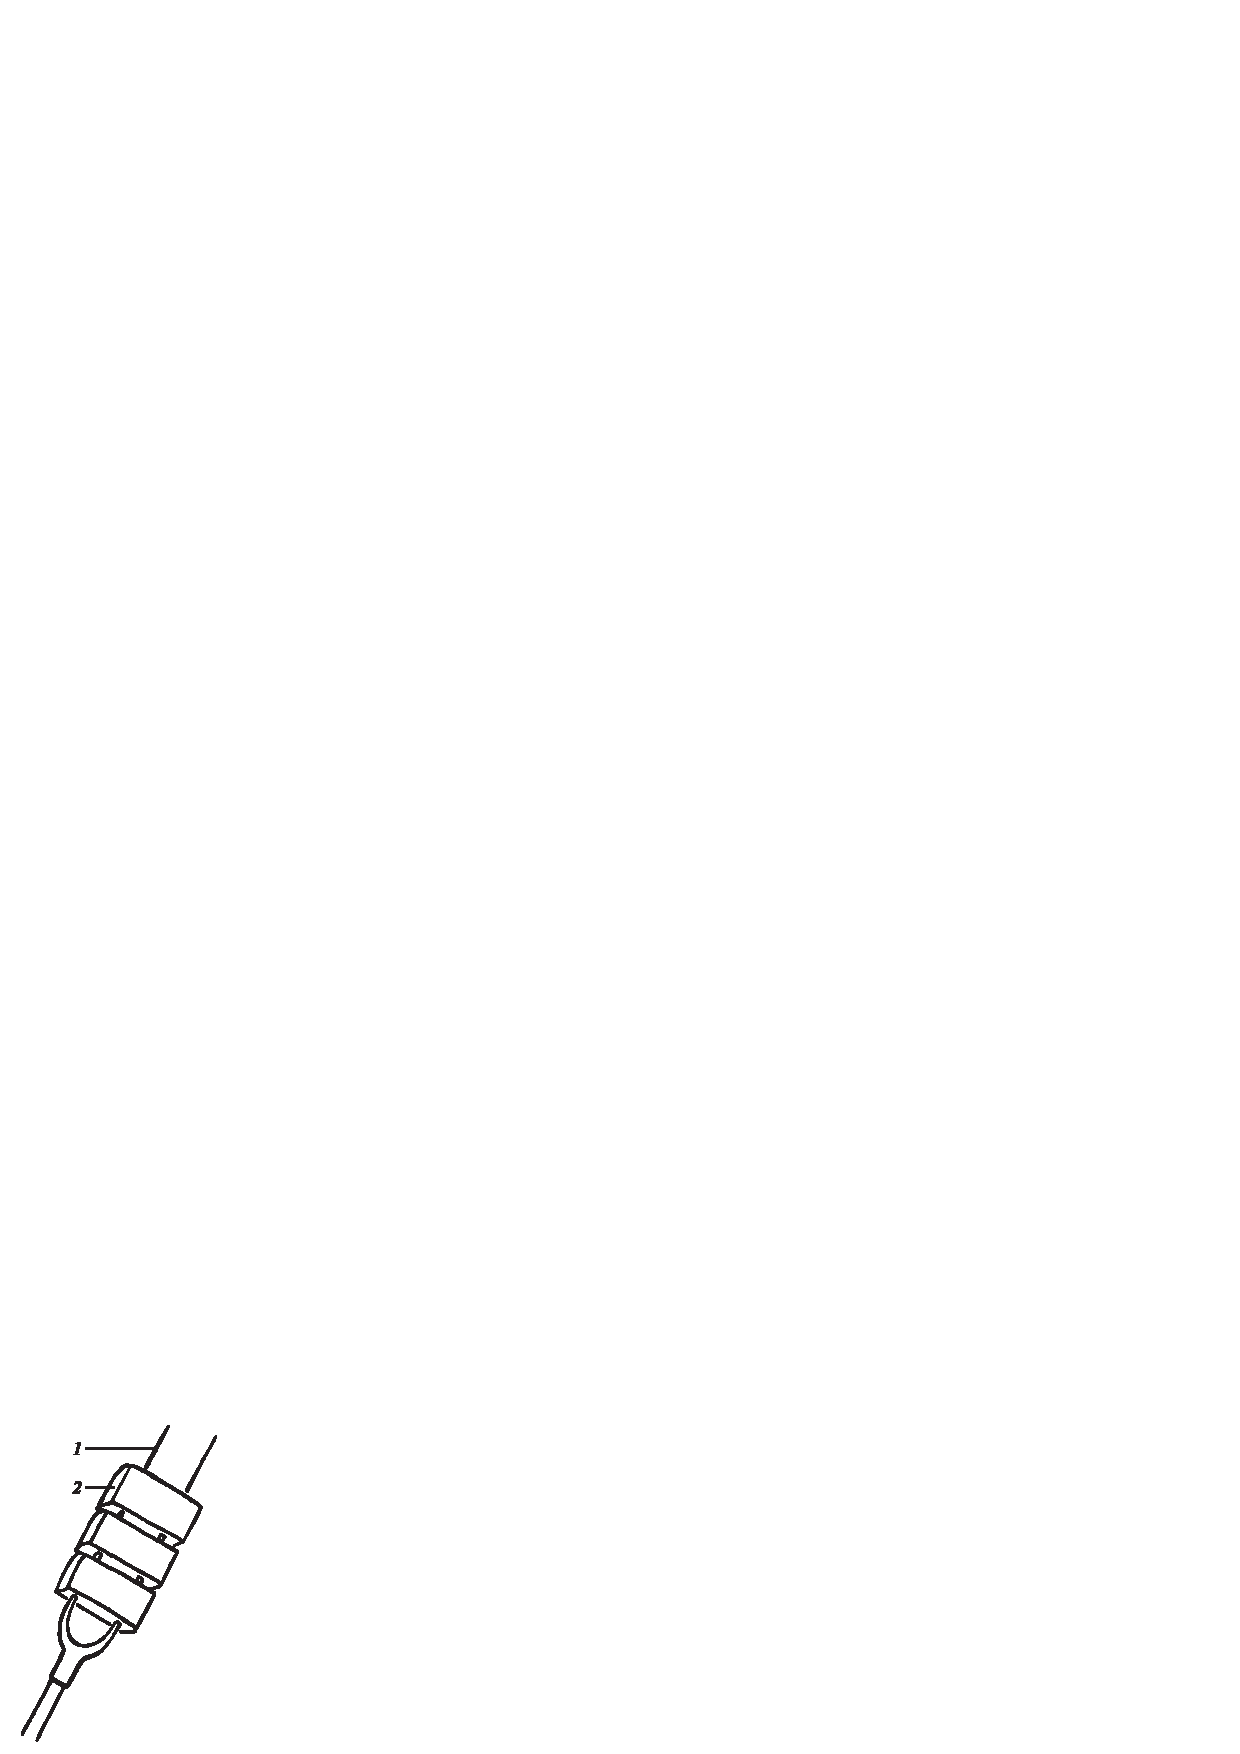
\includegraphics[scale=1]{illustration-011.pdf}%
\vspace{-.4375\baselineskip}%
\caption{叉烧宣腿叉法}
\label{method of fork roasting ham}%
\begingroup%
\small%
\noindent%
\null\hspace{0em}1. 铁叉 2. 火腿
\endgroup%
\end{wrapfigure}

\step 用刀将火腿均匀地切为三块,每块切成一寸三分宽、四寸半长,厚度为火腿本身的
厚度,用铁叉平叉起来(如图~\ref{method of fork roasting ham}\,)。将蛋清与豆粉
调匀,涂于叉起来的火腿上以保持原味,而免烧时走油走味。

\step 把杠炭三斤放入平炉上烧红,而后把叉好的火腿在平炉上以微火烘烤,要反复转动
叉柄,约二十分钟,烤至火腿熟透心时,揩净叉尖后取下叉子。用刀把火腿每隔两分远切
一刀,但不要完全切断,使其不会分开。然后摆在盘中,下面摆两块、上面摆一块成为
“品”字形。与烤熟的面包(切为十二片)和蒸好的荷叶饼同时上席。

\features

此菜外酥内香,为下酒的好菜。

\end{recipe}

% vim: filetype=tex noautoindent nojoinspaces
% vim: fileencoding=utf-8 formatoptions+=m
% vim: textwidth=78 tabstop=4 shiftwidth=4 softtabstop=4

\begin{recipe}{炸溜田鸡腿}

\ingredients

\ingredient{田鸡}{十五个}
\ingredient{鸡蛋}{一个}
\ingredient{干豆粉}{二钱}
\ingredient{盐}{二分}
\ingredient{酱油}{二钱}
\ingredient{姜片}{一钱}
\ingredient{葱}{二钱}
\ingredient{泡海椒}{二根}
\ingredient{料酒}{二钱}
\ingredient{胡椒面}{一分}
\ingredient{化猪油}{四两}
\ingredient{水豆粉}{一钱}

\cooking

\step 	将田鸡剐后洗净,取下后两腿备用。泡海椒、葱切成 马耳形。

\step 	蛋清、豆粉、盐调匀,将田鸡腿拌匀;豆油、姜片、 马耳葱、泡海椒节、料酒、胡椒面加水豆粉调成滋汁备用。

待油锅热后,将田鸡腿放入锅内浸炸,待油浸透后, 起锅去骨,又将田鸡腿放入锅内,将滋汁加热汤少许倒于田 鸡腿上,搅匀起锅即成。

\notes

鲜嫩,味美,席桌热碟之一。

\end{recipe}

% vim: filetype=tex noautoindent
% vim: fileencoding=utf-8
% vim: textwidth=78 tabstop=4 shiftwidth=4 softtabstop=4

% BSD 3-Clause License
%
% Copyright (c) 2023 Quux System and Technology. All rights reserved.
%
% Redistribution and use in source and binary forms, with or without
% modification, are permitted provided that the following conditions are met:
%
% 1. Redistributions of source code must retain the above copyright notice, this
%    list of conditions and the following disclaimer.
%
% 2. Redistributions in binary form must reproduce the above copyright notice,
%    this list of conditions and the following disclaimer in the documentation
%    and/or other materials provided with the distribution.
%
% 3. Neither the name of the copyright holder nor the names of its
%    contributors may be used to endorse or promote products derived from
%    this software without specific prior written permission.
%
% THIS SOFTWARE IS PROVIDED BY THE COPYRIGHT HOLDERS AND CONTRIBUTORS "AS IS"
% AND ANY EXPRESS OR IMPLIED WARRANTIES, INCLUDING, BUT NOT LIMITED TO, THE
% IMPLIED WARRANTIES OF MERCHANTABILITY AND FITNESS FOR A PARTICULAR PURPOSE ARE
% DISCLAIMED. IN NO EVENT SHALL THE COPYRIGHT HOLDER OR CONTRIBUTORS BE LIABLE
% FOR ANY DIRECT, INDIRECT, INCIDENTAL, SPECIAL, EXEMPLARY, OR CONSEQUENTIAL
% DAMAGES (INCLUDING, BUT NOT LIMITED TO, PROCUREMENT OF SUBSTITUTE GOODS OR
% SERVICES; LOSS OF USE, DATA, OR PROFITS; OR BUSINESS INTERRUPTION) HOWEVER
% CAUSED AND ON ANY THEORY OF LIABILITY, WHETHER IN CONTRACT, STRICT LIABILITY,
% OR TORT (INCLUDING NEGLIGENCE OR OTHERWISE) ARISING IN ANY WAY OUT OF THE USE
% OF THIS SOFTWARE, EVEN IF ADVISED OF THE POSSIBILITY OF SUCH DAMAGE.
%
\begin{recipe}{五彩土司}

\ingredients

\ingredient{土司}{一磅}
\ingredient{鲜鱼肉}{八两}
\ingredient{猪肥膘}{二两}
\ingredient{鸡蛋}{五个}
\ingredient{熟瘦火腿}{五钱}
\ingredient{水发木耳}{五钱}
\ingredient{花椒面}{二分}
\ingredient{豆粉}{三钱}
\ingredient{芝麻}{五钱}
\ingredient{绿色小菜}{一两}
\ingredient{香油}{五钱}
\ingredient{蕃茄酱}{五钱}
\ingredient{生菜}{三两}
\ingredient{白糖}{三钱}
\ingredient{醋}{三钱}
\ingredient{盐}{五分}
\ingredient{菜油}{二斤耗一两五}

\preparation

\step 鲜鱼剔骨,去皮,选净细刺后,与肥膘分别用刀背砸茸搅成“鱼糁”。摊蛋皮一
张,连同火腿、木耳、绿色小菜分别切成各种细末,连芝麻共成五种细末各分装一边。

\step 土司修去周围的皮后,切成二分厚的片,先在一面抹上一层“蛋清豆粉”再放上“鱼
糁”约三分厚抹平,再将五种细末一样样摊开在墩子上,分颜色用刀口刮成一字条形,顺
着贴在“糁”上约一分厚,用手按平不脱,自成五色,每片同样贴好,上笼蒸五分钟取出。

\step 锅内掺油在旺火上烧至七成火,将土司放入,贴细末一面向上,炸成金黄色,将油
滗尽,淋上香油搛起;再用刀改成五分宽、一寸二长的条子(切时按五色切开使每片都现
彩色),装在条盘的一端,另一端放生菜。走菜时随椒盐一碟同上。

\features

色分五彩,美观;味兼香、酥、脆、嫩,为席桌行菜之一。

\end{recipe}

% vim: filetype=tex noautoindent nojoinspaces
% vim: fileencoding=utf-8 formatoptions+=m
% vim: textwidth=78 tabstop=4 shiftwidth=4 softtabstop=4

% BSD 3-Clause License
%
% Copyright (c) 2023 Quux System and Technology. All rights reserved.
%
% Redistribution and use in source and binary forms, with or without
% modification, are permitted provided that the following conditions are met:
%
% 1. Redistributions of source code must retain the above copyright notice, this
%    list of conditions and the following disclaimer.
%
% 2. Redistributions in binary form must reproduce the above copyright notice,
%    this list of conditions and the following disclaimer in the documentation
%    and/or other materials provided with the distribution.
%
% 3. Neither the name of the copyright holder nor the names of its
%    contributors may be used to endorse or promote products derived from
%    this software without specific prior written permission.
%
% THIS SOFTWARE IS PROVIDED BY THE COPYRIGHT HOLDERS AND CONTRIBUTORS "AS IS"
% AND ANY EXPRESS OR IMPLIED WARRANTIES, INCLUDING, BUT NOT LIMITED TO, THE
% IMPLIED WARRANTIES OF MERCHANTABILITY AND FITNESS FOR A PARTICULAR PURPOSE ARE
% DISCLAIMED. IN NO EVENT SHALL THE COPYRIGHT HOLDER OR CONTRIBUTORS BE LIABLE
% FOR ANY DIRECT, INDIRECT, INCIDENTAL, SPECIAL, EXEMPLARY, OR CONSEQUENTIAL
% DAMAGES (INCLUDING, BUT NOT LIMITED TO, PROCUREMENT OF SUBSTITUTE GOODS OR
% SERVICES; LOSS OF USE, DATA, OR PROFITS; OR BUSINESS INTERRUPTION) HOWEVER
% CAUSED AND ON ANY THEORY OF LIABILITY, WHETHER IN CONTRACT, STRICT LIABILITY,
% OR TORT (INCLUDING NEGLIGENCE OR OTHERWISE) ARISING IN ANY WAY OUT OF THE USE
% OF THIS SOFTWARE, EVEN IF ADVISED OF THE POSSIBILITY OF SUCH DAMAGE.
%
\begin{recipe}{兰花吐司}

\ingredients

\ingredient{吐司}{一磅}
\ingredient{肥膘}{二两}
\ingredient{鸡蛋清}{四个}
\ingredient{肫肝}{四个}
\ingredient{鲜鱼}{八两}
\ingredient{盐}{四分}
\ingredient{味精}{二分}
\ingredient{干豆粉}{五钱}
\ingredient{香油}{五钱}
\ingredient{葱白}{一两}
\ingredient{料酒}{二钱}
\ingredient{白糖}{一钱}
\ingredient{菜油}{一斤耗一两五}
\ingredient{甜酱}{三钱}

\preparation

\step 吐司切成三分厚片子(共四片),鲜鱼打成“鱼糁”,每个吐司片上先抹蛋清豆粉,
再涂上鱼糁,用手抹平整。

\step 肫肝四个去掉两面皮子,每个剞为六个鸡冠花的形式(共二十四个),用盐、料酒
少许,抹匀后分别插在吐司上(每片六个分两边插),上笼蒸五分钟取出晾冷,每片吐司
再开为六片待用。

\step 菜油在旺火上烧至七成火候,将吐司倒入锅内炸至浅黄色,将油滗去,淋上香油,
簸匀起锅入盘。

\step 白糖、香油、葱白、甜酱,兑成葱酱,镶入盘另一端入席。

\features

美观,酥脆,席桌行菜,下酒最宜。

\end{recipe}

% vim: filetype=tex noautoindent nojoinspaces
% vim: fileencoding=utf-8 formatoptions+=m
% vim: textwidth=78 tabstop=4 shiftwidth=4 softtabstop=4

\begin{recipe}{杏圆土司}

\ingredients

\ingredient{土司}{一磅}
\ingredient{鸡蛋}{四个}
\ingredient{净鲜鱼肉}{四两}
\ingredient{猪肥膘肉}{二两}
\ingredient{干豆粉}{五钱}
\ingredient{化猪油}{二斤耗二两}
\ingredient{生菜}{三两}
\ingredient{香油}{五钱}
\ingredient{白糖}{三钱}
\ingredient{醋}{三钱}
\ingredient{盐}{四分}
\ingredient{味精}{三分}
\ingredient{料酒}{二钱}

\preparation

\step 土司切成一分半厚的大片,再将大片改成八分见方的小片,共切三十片,修去四角
成八分过心的圆形,放入盘内待用。

\step 将鲜鱼肉、猪肥膘分别捶茸,加鸡蛋清、盐、水豆粉打成“鱼糁”放在碗内待用。

\step 每一片土司上均匀地放上二分厚的鱼糁,用手刮边沿成中心高边沿低的形式,一直
做完三十片。

\step 将锅置于旺火,倒入化猪油,烧至四成火,再一个个地放下土司(糁向上,土司向
下),由低温到高温,土司的颜色接近黄色(形色同杏圆相似),泌去锅内炸油,淋入香
油,起锅入条盘的一端。再将生菜淘洗干净,滤干水份,拌入糖、醋、香油、味精,放在
杏圆土司的另一端即成。

\features

酥、香、脆、嫩,在席桌中宜于行菜。

\end{recipe}

% vim: filetype=tex noautoindent nojoinspaces
% vim: fileencoding=utf-8 formatoptions+=m
% vim: textwidth=78 tabstop=4 shiftwidth=4 softtabstop=4

% BSD 3-Clause License
%
% Copyright (c) 2023 Quux System and Technology. All rights reserved.
%
% Redistribution and use in source and binary forms, with or without
% modification, are permitted provided that the following conditions are met:
%
% 1. Redistributions of source code must retain the above copyright notice, this
%    list of conditions and the following disclaimer.
%
% 2. Redistributions in binary form must reproduce the above copyright notice,
%    this list of conditions and the following disclaimer in the documentation
%    and/or other materials provided with the distribution.
%
% 3. Neither the name of the copyright holder nor the names of its
%    contributors may be used to endorse or promote products derived from
%    this software without specific prior written permission.
%
% THIS SOFTWARE IS PROVIDED BY THE COPYRIGHT HOLDERS AND CONTRIBUTORS "AS IS"
% AND ANY EXPRESS OR IMPLIED WARRANTIES, INCLUDING, BUT NOT LIMITED TO, THE
% IMPLIED WARRANTIES OF MERCHANTABILITY AND FITNESS FOR A PARTICULAR PURPOSE ARE
% DISCLAIMED. IN NO EVENT SHALL THE COPYRIGHT HOLDER OR CONTRIBUTORS BE LIABLE
% FOR ANY DIRECT, INDIRECT, INCIDENTAL, SPECIAL, EXEMPLARY, OR CONSEQUENTIAL
% DAMAGES (INCLUDING, BUT NOT LIMITED TO, PROCUREMENT OF SUBSTITUTE GOODS OR
% SERVICES; LOSS OF USE, DATA, OR PROFITS; OR BUSINESS INTERRUPTION) HOWEVER
% CAUSED AND ON ANY THEORY OF LIABILITY, WHETHER IN CONTRACT, STRICT LIABILITY,
% OR TORT (INCLUDING NEGLIGENCE OR OTHERWISE) ARISING IN ANY WAY OUT OF THE USE
% OF THIS SOFTWARE, EVEN IF ADVISED OF THE POSSIBILITY OF SUCH DAMAGE.
%
\begin{recipe}{酿冬菇}

\ingredients

\ingredient{干冬菇}{三两}
\ingredient{盐}{一钱}
\ingredient{熟火腿}{六钱}
\ingredient{鸡蛋清}{四个}
\ingredient{黄秧白菜心}{一两}
\ingredient{葱白}{二钱}
\ingredient{干豆粉}{一两}
\ingredient{酱油}{四钱五}
\ingredient{姜}{二钱}
\ingredient{鸡脯肉}{二两五}
\ingredient{水豆粉}{六钱}
\ingredient{化猪油}{二两}
\ingredient{胡椒面}{二分五}
\ingredient{鸡油}{六钱}
\ingredient{猪肥膘肉}{一两五}
\ingredient{味精}{三分}
\ingredient{鸡汤}{四两}
\ingredient{料酒}{一两}
\ingredient{冬笋(净)}{一两}

\preparation

\step 干冬菇选菌盖直径约八分,大小均匀的二十四朵,用清水一大碗泡半小时,至泡胀
而未全胀时滗去水(另作他用)。换清水用手指在冬菇周围凸凹不平地方掏去泥沙,淘洗
干净,用刀齐盖底切去茎(作别用);然后放在沸水中煮约十分钟,端离火口浸泡十分钟
捞出;再换清水烧沸同样再煮一次,滗去煮水不用。此时菌盖直径已发胀至一寸二分左
右,则已干净胀透。

猪油倒入炒锅内,在旺火上烧至五成热,将葱白段、姜(去皮、拍松)、盐、料酒、鸡汤
依次放入,再加入冬菇、味精、胡椒面同烧五分钟,使冬菇入味,将汤滗去,把冬菇捞入
筲箕中,将水滤干后放盘中摊开,切去茎的一面,向上摆好待用。

\step 鸡脯肉去掉外面一层白膜,在菜墩上用刀背捶成茸,边捶边用刀口刮去肉内白筋,
捶至极细为止。猪肥膘肉用刀剁成肉泥(肉泥如同油脂,但不能化油;热天为了避免在剁
时化油,可先将肥膘肉放在冰箱内冰冻后再用,因化油要影响搅成糁)。大碗内放入清
水,把鸡茸投入用竹筷顺着一定方向搅打五分钟,要搅散搅匀;随后放入鸡蛋清继续用力
同样搅打十分钟;再加入盐、味精、料酒、水豆粉,同时加入肥肉泥,用力搅打五分钟成
稀糊状(用筷蘸一点滴在清水面上不沉底),即成鸡糁。

鸡蛋清二个与干豆粉调匀成为蛋清豆粉,在盘中摆好的每个冬菇上的凹处抹上一层,再用
调羹舀着鸡糁填满,随用调羹刮平。然后装入蒸笼内(有糁一面向上)上笼蒸五分钟,熟
后取出待用(临用时才取,以保持热度)。

\step 火腿、冬笋切成长一寸三、宽三分、厚半分的片。黄秧白菜心切成一寸半大小的
块。猪油放入炒锅内,在旺火上烧至五成热,即放入切好的火腿、冬笋、黄秧白菜,用汤
瓢翻搅两下,再迅速加入料酒、盐、酱油、鸡汤、味精、胡椒面等佐料,用汤瓢搅匀。同
时把蒸熟的冬菇翻入盘内(要使冬菇盖顶向上),即用水豆粉将汁勾芡,淋入鸡油,再把
汁全部淋于冬菇面上即成。

\features

此菜冬菇细嫩松脆,菌香味特浓,鲜美可口。

\end{recipe}

% vim: filetype=tex noautoindent nojoinspaces
% vim: fileencoding=utf-8 formatoptions+=m
% vim: textwidth=78 tabstop=4 shiftwidth=4 softtabstop=4

% BSD 3-Clause License
%
% Copyright (c) 2023 Quux System and Technology. All rights reserved.
%
% Redistribution and use in source and binary forms, with or without
% modification, are permitted provided that the following conditions are met:
%
% 1. Redistributions of source code must retain the above copyright notice, this
%    list of conditions and the following disclaimer.
%
% 2. Redistributions in binary form must reproduce the above copyright notice,
%    this list of conditions and the following disclaimer in the documentation
%    and/or other materials provided with the distribution.
%
% 3. Neither the name of the copyright holder nor the names of its
%    contributors may be used to endorse or promote products derived from
%    this software without specific prior written permission.
%
% THIS SOFTWARE IS PROVIDED BY THE COPYRIGHT HOLDERS AND CONTRIBUTORS "AS IS"
% AND ANY EXPRESS OR IMPLIED WARRANTIES, INCLUDING, BUT NOT LIMITED TO, THE
% IMPLIED WARRANTIES OF MERCHANTABILITY AND FITNESS FOR A PARTICULAR PURPOSE ARE
% DISCLAIMED. IN NO EVENT SHALL THE COPYRIGHT HOLDER OR CONTRIBUTORS BE LIABLE
% FOR ANY DIRECT, INDIRECT, INCIDENTAL, SPECIAL, EXEMPLARY, OR CONSEQUENTIAL
% DAMAGES (INCLUDING, BUT NOT LIMITED TO, PROCUREMENT OF SUBSTITUTE GOODS OR
% SERVICES; LOSS OF USE, DATA, OR PROFITS; OR BUSINESS INTERRUPTION) HOWEVER
% CAUSED AND ON ANY THEORY OF LIABILITY, WHETHER IN CONTRACT, STRICT LIABILITY,
% OR TORT (INCLUDING NEGLIGENCE OR OTHERWISE) ARISING IN ANY WAY OUT OF THE USE
% OF THIS SOFTWARE, EVEN IF ADVISED OF THE POSSIBILITY OF SUCH DAMAGE.
%
\begin{recipe}{软炸口蘑}

\ingredients

\ingredient{口蘑}{二两五}
\ingredient{猪油}{一斤约耗三两}
\ingredient{鸡蛋清}{三个}
\ingredient{鸡汤}{五两}
\ingredient{盐}{六分}
\ingredient{干豆粉}{一两}
\ingredient{味精}{二分}
\ingredient{料酒}{六钱}
\ingredient{姜}{二钱}
\ingredient{胡椒面}{一分五}
\ingredient{葱}{二钱}
\ingredient{香油}{二钱}
\ingredient{蕃茄酱}{二两}
\ingredient{白糖}{少许}

\preparation

\step 口蘑选用大小均匀的,用清水泡半小时滗去水作别用,再换清水淘洗去泥沙。洗净
后用沸水煮十分钟,而后再换水煮十分钟,发至胀透,即成水发口蘑。鸡蛋清与豆粉调成
干湿适度的蛋清豆粉。

\step 猪油放入锅内,在旺火上烧至五成热,放入葱、姜稍煸,即依次加入鸡汤、口蘑、
料酒、盐、味精、胡椒面等烧约八分钟,用汤瓢将口蘑捞出,入筲箕内滤干水,放入蛋清
豆粉内拌匀,使每块口蘑都能裹上一层。

\step 猪油放入锅内,于旺火上烧至五成热,将裹好蛋清豆粉的口蘑逐个放入稍炸。若火
过旺即将锅端离火口,炸至口蘑上的蛋清豆粉刚熟(看不见黄色仍是白的)即捞入盘中。
要边放边捞,以免炸糊。若有粘连,可用手掰开。再将锅在旺火上烧至八成热,将盘中炸
过的口蘑全部倒入,约炸五分钟呈金黄色时滗去炸油,随即淋入香油,捞出盛入盘中。另
以四个小碟盛入蕃茄酱(蕃茄酱加香油、白糖、味精、盐各少许)蘸食。

\features

此菜口蘑皮酥内嫩,清香可口。

另一制作法:不裹蛋清豆粉而用糁裹口蘑,味更鲜嫩。如用糁,原料上须增加鸡肉二两
五或鱼肉半斤、肥膘肉四两,作打糁用。

\end{recipe}

% vim: filetype=tex noautoindent nojoinspaces
% vim: fileencoding=utf-8 formatoptions+=m
% vim: textwidth=78 tabstop=4 shiftwidth=4 softtabstop=4

% BSD 3-Clause License
%
% Copyright (c) 2023 Quux System and Technology. All rights reserved.
%
% Redistribution and use in source and binary forms, with or without
% modification, are permitted provided that the following conditions are met:
%
% 1. Redistributions of source code must retain the above copyright notice, this
%    list of conditions and the following disclaimer.
%
% 2. Redistributions in binary form must reproduce the above copyright notice,
%    this list of conditions and the following disclaimer in the documentation
%    and/or other materials provided with the distribution.
%
% 3. Neither the name of the copyright holder nor the names of its
%    contributors may be used to endorse or promote products derived from
%    this software without specific prior written permission.
%
% THIS SOFTWARE IS PROVIDED BY THE COPYRIGHT HOLDERS AND CONTRIBUTORS "AS IS"
% AND ANY EXPRESS OR IMPLIED WARRANTIES, INCLUDING, BUT NOT LIMITED TO, THE
% IMPLIED WARRANTIES OF MERCHANTABILITY AND FITNESS FOR A PARTICULAR PURPOSE ARE
% DISCLAIMED. IN NO EVENT SHALL THE COPYRIGHT HOLDER OR CONTRIBUTORS BE LIABLE
% FOR ANY DIRECT, INDIRECT, INCIDENTAL, SPECIAL, EXEMPLARY, OR CONSEQUENTIAL
% DAMAGES (INCLUDING, BUT NOT LIMITED TO, PROCUREMENT OF SUBSTITUTE GOODS OR
% SERVICES; LOSS OF USE, DATA, OR PROFITS; OR BUSINESS INTERRUPTION) HOWEVER
% CAUSED AND ON ANY THEORY OF LIABILITY, WHETHER IN CONTRACT, STRICT LIABILITY,
% OR TORT (INCLUDING NEGLIGENCE OR OTHERWISE) ARISING IN ANY WAY OUT OF THE USE
% OF THIS SOFTWARE, EVEN IF ADVISED OF THE POSSIBILITY OF SUCH DAMAGE.
%
\begin{recipe}{海味什锦}

\ingredients

\ingredient{熟鸡肉}{一两五}
\ingredient{猪心子}{一两五}
\ingredient{猪舌}{一两五}
\ingredient{猪肚}{一两五}
\ingredient{环喉}{三根}
\ingredient{蹄筋}{三根}
\ingredient{冬笋}{一两五}
\ingredient{脊髓}{一两五}
\ingredient{口蘑}{三钱}
\ingredient{水发海参}{二两}
\ingredient{水发鱿鱼}{二两}
\ingredient{珧柱}{三钱}
\ingredient{熟火腿}{三钱}
\ingredient{金钩}{三钱}
\ingredient{菜心}{五两}
\ingredient{酱油}{四钱}
\ingredient{糖汁}{少许}
\ingredient{化猪油}{二两}
\ingredient{胡椒}{一分}
\ingredient{料酒}{五钱}
\ingredient{盐}{五分}
\ingredient{水豆粉}{五钱}
\ingredient{花椒}{数颗}
\ingredient{鸡汤}{三斤}
\ingredient{姜、葱}{各少许}

\preparation

\step 先将海参、鱿鱼、火腿切成二寸长、五分宽的片。以上的原料除去珧柱、金钩外切
成大一字形条。脊髓用沸水汆过。海参、鱿鱼同样用沸水分开汆过。菜心泹后用清水漂起
待用。

\step 珧柱放在蒸碗内上笼大火蒸𤆵,将锅放在旺火上,放下猪油,再放入姜葱,爆出香
味后,倒入鸡汤、盐、糖汁、料酒、酱油、花椒、胡椒及以上用沸水汆过的原材料(除鱿
鱼、海参、脊髓、小菜外)小火烧𤆵。再将小菜泹𤆵后,在白油锅内煸过,起锅垫入走菜
盘内。再将烧𤆵后的一字条,捞入盘内放在小菜上边。鱿鱼、脊髓,放在烧一字条等原料
的原汁内,烧上味打入盘内放在一字条块上边。再放入海参于原汁内烧上味,勾入豆粉,
起锅淋入盘内,海参放在鱿鱼、脊髓上面上席。

\features

美观大方,味浓可口,适宜四季头菜。

\end{recipe}

% vim: filetype=tex noautoindent nojoinspaces
% vim: fileencoding=utf-8 formatoptions+=m
% vim: textwidth=78 tabstop=4 shiftwidth=4 softtabstop=4

\pagebreak
% BSD 3-Clause License
%
% Copyright (c) 2023 Quux System and Technology. All rights reserved.
%
% Redistribution and use in source and binary forms, with or without
% modification, are permitted provided that the following conditions are met:
%
% 1. Redistributions of source code must retain the above copyright notice, this
%    list of conditions and the following disclaimer.
%
% 2. Redistributions in binary form must reproduce the above copyright notice,
%    this list of conditions and the following disclaimer in the documentation
%    and/or other materials provided with the distribution.
%
% 3. Neither the name of the copyright holder nor the names of its
%    contributors may be used to endorse or promote products derived from
%    this software without specific prior written permission.
%
% THIS SOFTWARE IS PROVIDED BY THE COPYRIGHT HOLDERS AND CONTRIBUTORS "AS IS"
% AND ANY EXPRESS OR IMPLIED WARRANTIES, INCLUDING, BUT NOT LIMITED TO, THE
% IMPLIED WARRANTIES OF MERCHANTABILITY AND FITNESS FOR A PARTICULAR PURPOSE ARE
% DISCLAIMED. IN NO EVENT SHALL THE COPYRIGHT HOLDER OR CONTRIBUTORS BE LIABLE
% FOR ANY DIRECT, INDIRECT, INCIDENTAL, SPECIAL, EXEMPLARY, OR CONSEQUENTIAL
% DAMAGES (INCLUDING, BUT NOT LIMITED TO, PROCUREMENT OF SUBSTITUTE GOODS OR
% SERVICES; LOSS OF USE, DATA, OR PROFITS; OR BUSINESS INTERRUPTION) HOWEVER
% CAUSED AND ON ANY THEORY OF LIABILITY, WHETHER IN CONTRACT, STRICT LIABILITY,
% OR TORT (INCLUDING NEGLIGENCE OR OTHERWISE) ARISING IN ANY WAY OUT OF THE USE
% OF THIS SOFTWARE, EVEN IF ADVISED OF THE POSSIBILITY OF SUCH DAMAGE.
%
\begin{recipe}{生片菊花锅}

\ingredients

\ingredient{鲫鱼}{八两}
\ingredient{胡椒}{三分}
\ingredient{粉条}{二钱}
\ingredient{油炸花生米}{一两五}
\ingredient{生鸡脯肉}{三两}
\ingredient{盐}{三分}
\ingredient{豌豆尖}{三两}
\ingredient{油条}{三根}
\ingredient{奶汤}{二斤半}
\ingredient{香菜}{一两}
\ingredient{干粉}{五钱}
\ingredient{菜油}{一斤耗三两}
\ingredient{葱}{二钱}
\ingredient{白菜心}{三两}
\ingredient{鸡𬂁肝}{三个}
\ingredient{味精}{三分}
\ingredient{菠菜}{五两}
\ingredient{猪腰}{四两}
\ingredient{化猪油}{一两}
\ingredient{姜}{二钱}
\ingredient{粗撒子}{二把}
\ingredient{白菊花}{一朵}

\preparation

\step 鲫鱼洗净,去鳞,去肠杂,去刺(刺留用),用刀切成二寸长、一分厚、宽同鱼身
的薄片。鸡𬂁肝洗净,去表皮,切成薄片。生鸡脯肉片为一寸长、八分宽的薄片。猪腰去
筋和腰臊,切成鸡脯大小的薄片(以上薄片,愈薄愈好)。这四种片称为“四生片”,分别
摆于七寸盘中成风车形。

\step 菜油一斤入锅烧红,投入粉条,炸成黄色;花生米去皮;油条切成一寸长段;撒子
捏散(临上席时再用油炸一次以保持酥脆);分别放入七寸盘内,称为“四油酥”。

\step 白菜心洗净,用手撕去筋;豌豆尖淘洗,只留嫩苞;菠菜去老叶和茎根部分;香菜
洗净;分别放于七寸盘中,称为“四鲜菜”。

\step 姜一钱去皮,切成细末;葱切成葱花;与胡椒、味精共摆一碟,每样占碟的四分之
一。另以小碟盛盐备用。

\step 鲜菊花一大朵(最好为自色),用刀切去花蒂,抽出花蕊,仍以菊花原形放入盘
中。

\step 锅置火上,放入猪油,加入姜(拍松)、葱切成五分长的短节,随即放入奶汤和鱼
骨刺,烧沸,约五分钟捞去鱼骨刺和姜、葱,把汤舀入铜锅内为鱼羹汤。

\step 桌上放一粗瓷深盘,盘内盛酒精,盘上加铜架,架上放铜锅,吃时将酒精燃烧,锅
内汤沸时先将菊花放下,次将各类生肉、生菜分别于汤内烫熟吃(除生片、生菜外其余油
酥忌下锅内)。

\features

此菜宜于秋季吃,生片、鲜菜汤味清鲜,佐酒下饭均宜。菜内生片、鲜菜可按季节变动,
但只能用四样。冬季改用梅花,即名“梅花锅”。

\end{recipe}

% vim: filetype=tex noautoindent nojoinspaces
% vim: fileencoding=utf-8 formatoptions+=m
% vim: textwidth=78 tabstop=4 shiftwidth=4 softtabstop=4

\begin{recipe}{蝴蝶竹荪}

\ingredients

\ingredient{竹荪}{四钱}
\ingredient{鸡蛋}{五个}
\ingredient{鲜鱼肉}{四两}
\ingredient{肥膘肉}{二两}
\ingredient{鲜笋}{二两}
\ingredient{熟火腿}{一两}

\ingredient{黑芝麻}{一钱}
\ingredient{干豆粉}{五钱}
\ingredient{盐}{七分}
\ingredient{味精}{三分}
\ingredient{胡椒面}{二分}
\ingredient{料酒}{五钱}
\ingredient{酱油}{二钱}
\ingredient{猪瘦肉}{三两}
\ingredient{鸡脯肉}{三两}
\ingredient{清汤}{一斤半}
\ingredient{丝瓜}{三两}

\cooking

\step 	将竹荪用温水泡胀,换清水洗数次,放在墩子上用刀 修去两头,剖开成为六分宽、二寸长的片子,共四十八片;将 片的同一方向的两头修去呈半圆形,共修二十四片,余下的 二十四片用斜刀切断呈箭头形;将四十八片竹荪一并放入沸 水内汆过,泌去清水,用好汤喂一次,放入碗内装好待用。

\step 	鸡蛋摊成蛋皮;鲜笋煮熟放在碗内;丝瓜刮后车下皮, 洗净,切成二寸长的段,用沸水沮熟,用清水漂起;再将丝瓜 皮、蛋皮、鲜笋、火腿切成二寸长的二粗丝,分开装入盘 内。黑芝麻淘洗干净,捞起;半个蛋清拌成蛋清豆粉;鲜鱼 肉去净皮翅,用刀背反复捶茸(肉内不见籽为准);肥膘剁 细〔如油脂)。再将鱼茸放入瓢内,三个半蛋清,八钱清 水,三分盐、剁好的肥膘茸及水发湿的干豆粉打成“鱼糁” 装入碗内待用。

\step 	将修去边角的竹荪摆成蝴蝶形,中间抹上蛋清豆粉, 再将鱼糁刮于手心上呈尖刀形,约一寸五长,放于抹豆粉 处,二十四个照样摆完。再用铁夹将丝瓜火腿、蛋皮丝各 夹一丝入糁的中心,夹二根单丝插入糁的前面,放二粒芝麻 在糁的上边,二十四个一起做完即为蝴蝶竹荪。上笼蒸五分 钟即熟(用时馏热)。鸡脯肉、猪瘦肉分别捶成茸子,并用 清水解散,装入碗内。

\step 将锅放在旺火上,倒下一斤半清汤加酱油、胡椒、 盐,烧开后投入红茸子,推动数转,微开时打尽肉沫;再投 入白茸子,推动数转,微开时,同样打尽肉末,无杂质时, 放下味精,取出笼内的蝴蝶竹荪,用清汤过一次,翻入大汤 盘内,再将锅内的清汤灌入即成。

\notes

形色美丽,汤鲜味美,适宜春夏二季。

\end{recipe}

% vim: filetype=tex noautoindent
% vim: fileencoding=utf-8
% vim: textwidth=78 tabstop=4 shiftwidth=4 softtabstop=4

% BSD 3-Clause License
%
% Copyright (c) 2023 Quux System and Technology. All rights reserved.
%
% Redistribution and use in source and binary forms, with or without
% modification, are permitted provided that the following conditions are met:
%
% 1. Redistributions of source code must retain the above copyright notice, this
%    list of conditions and the following disclaimer.
%
% 2. Redistributions in binary form must reproduce the above copyright notice,
%    this list of conditions and the following disclaimer in the documentation
%    and/or other materials provided with the distribution.
%
% 3. Neither the name of the copyright holder nor the names of its
%    contributors may be used to endorse or promote products derived from
%    this software without specific prior written permission.
%
% THIS SOFTWARE IS PROVIDED BY THE COPYRIGHT HOLDERS AND CONTRIBUTORS "AS IS"
% AND ANY EXPRESS OR IMPLIED WARRANTIES, INCLUDING, BUT NOT LIMITED TO, THE
% IMPLIED WARRANTIES OF MERCHANTABILITY AND FITNESS FOR A PARTICULAR PURPOSE ARE
% DISCLAIMED. IN NO EVENT SHALL THE COPYRIGHT HOLDER OR CONTRIBUTORS BE LIABLE
% FOR ANY DIRECT, INDIRECT, INCIDENTAL, SPECIAL, EXEMPLARY, OR CONSEQUENTIAL
% DAMAGES (INCLUDING, BUT NOT LIMITED TO, PROCUREMENT OF SUBSTITUTE GOODS OR
% SERVICES; LOSS OF USE, DATA, OR PROFITS; OR BUSINESS INTERRUPTION) HOWEVER
% CAUSED AND ON ANY THEORY OF LIABILITY, WHETHER IN CONTRACT, STRICT LIABILITY,
% OR TORT (INCLUDING NEGLIGENCE OR OTHERWISE) ARISING IN ANY WAY OUT OF THE USE
% OF THIS SOFTWARE, EVEN IF ADVISED OF THE POSSIBILITY OF SUCH DAMAGE.
%
\begin{recipe}[酿龙凤翅]{酿两样}

\ingredients

\ingredient{仔鸡翅膀}{八对}
\ingredient{生猪排骨}{十六节}
\ingredient{鲜笋}{四两}
\ingredient{熟火腿}{二两}
\ingredient{水发冬菇}{二两}
\ingredient{鲜菜}{三两}
\ingredient{冰糖}{五钱}
\ingredient{酱油}{一两}
\ingredient{料酒}{五钱}
\ingredient{味精}{三分}
\ingredient{水豆粉}{三钱}
\ingredient{香油}{二钱}
\ingredient{化鸡油}{三钱}
\ingredient{盐}{三分}
\ingredient{姜}{三钱}
\ingredient{葱}{五钱}
\ingredient{清汤}{二斤}
\ingredient{化猪油}{二两}
\ingredient{生鸡、猪骨}{一斤}
\ingredient{胡椒面}{一分}

\preparation

\step 选好八对仔鸡翅后,用清水洗净粗皮,夹净细毛,在锅内煮熟,用清水冰冷;再放
至墩子上,从弯处切断,两头不用只要第二节。又选大生猪排十六节,二寸五长,在汤锅
内煮熟待用。

\step 鲜笋煮熟后切成一寸五长的头粗丝。火腿、冬菇,切成同样的一字条,分开放在盘
内;再抽去鸡翅及猪排的扦子骨;用铁夹将火腿、鲜笋、冬菇各夹一丝入抽去扦子骨处,
即成龙凤翅(鸡翅为凤,猪排为龙),放入盘内待用。

\step 生鸡、猪骨,用清水洗净,除去血水,放入罐内;龙凤翅放于罐内生鸡骨上面。

\step 炒锅放于旺火上,放下化猪油及糖,炒成糖汁,呈金黄色。再倒入清汤二斤,将糖
汁冲散,倒入盛龙凤翅的罐内,加入酱油、料酒、盐、老姜(拍破)、葱(捆成把);将
罐在小火上烧四十分钟左右(汤烧至一半以上),龙凤翅已𤆵,提离火口,捞起龙凤翅于
二鱼碗内,龙凤各占碗的一半。罐内的汤灌入二鱼碗内(留一半待用),放入笼内大火蒸
三十分钟待用。

\step 鲜菜洗净后炒熟放于碗内,再放化猪油于锅内,倒入罐内余的一半原汁、一分胡
椒、三分味精,水豆粉勾芡,再取出笼内的装龙凤翅的碗,将生菜放在碗的上边,再翻入
大圆盘内,淋入三钱化鸡油,余下的鸡油及香油二钱一并投入锅内,起锅将原汁淋于龙凤
翅上即成。

\features

味浓𤆵香,色美,四季可口,席桌走行菜。

\end{recipe}

% vim: filetype=tex noautoindent nojoinspaces
% vim: fileencoding=utf-8 formatoptions+=m
% vim: textwidth=78 tabstop=4 shiftwidth=4 softtabstop=4

\end{tocminipageright}

\addtocounter{chapter}{2000}%
\addtocontents{toc}{\protect\enlargethispage{.5\baselineskip}}%
\category{重庆市部分菜肴}
\setlength{\cookbookafterrecipeskip}{.6875\baselineskip plus 1.1875\baselineskip}%

\begin{tocminipageleft}
\begingroup
\raggedbottom
\vspace{.25\baselineskip}
\begin{recipe}{烧牛头方}

\ingredients

\ingredient{水牛脑顶肉}{(不宜}
\ingredient{用黄牛)}{六斤}

\ingredient{冰糖色}{七钱}
\ingredient{母鸡汤(炒菜柏)}{三杓}

\ingredient{肉汤(炒菜杓)}{三杓}
\ingredient{鲜菜(或心)}{一斤}
\ingredient{绍酒}{一两二}
\ingredient{生鸡油}{一两二}
\ingredient{姜、葱}{少许}
\ingredient{食盐}{少许}
\ingredient{小磨麻油}{少许}
\ingredient{猪油}{五钱}

\cooking

烧牛头系取用其皮子。先将脑顶肉在炉火上将毛烧掉,

刮洗干净,用清水以文火炖约五小时,取出削净毛眼和肉取 其皮子。再将皮子用清水以文火烛至七成火候时(约需六小 时),即取出洗净,切成骨牌块状,用沸水连续微煮三次 (:厨称出水三次),以去其胶质和骚气。

猪油在旺火上煎辣,即放入葱姜快炒一、二铲,掺进肉 汤,俟汤沸即取出葱姜不要。随即放入牛皮移置文火上烧约 一小时,捞起滤干汤汁,置锑锅内,加进鸡汤、绍酒、生鸡 油、食盐和冰糖色等,以文火烧熟为止(约一小时)。起锅时 取出生鸡油渣不要,牛皮转入另一耳锅里用武火收稠汤汁, 淋上小磨麻油,盛于盘内,配上刚炒好的鲜菜即成。

\notes

味浓厚可口,质糯而不粘,色泽光亮,营养丰富,具有

\end{recipe}

% vim: filetype=tex noautoindent
% vim: fileencoding=utf-8
% vim: textwidth=78 tabstop=4 shiftwidth=4 softtabstop=4

\endgroup
\begin{recipe}{烟熏排骨}

\ingredients

\ingredient{猪签子排骨(正肋条)}{}
\ingredient{二斤}{}

\ingredient{小磨麻油}{二钱}
\ingredient{葱(切寸长小节V}{二根}

\ingredient{生姜(拍碎)}{三钱}
\ingredient{食盐}{一两}
\ingredient{柏枝}{五两}

\cooking

除去排骨边尖不整齐部分,以三根肋骨为一组宰成长方 形块子。两面均匀地抹上细盐,将姜、葱置排骨上盛在大碗 内,上蒸笼蒸约半小时,到刚熟时取出,放入沸热卤水(一 般卤菜的卤水)中煮到熟软的程度,即肉与骨稍用力便可使 之分离的时候取出。吃时油煎,热置文火上炸之,炸到油冒 出青烟即行取出,以鲜柏树枝烧烟熏约数分钟,刷上麻油, 砍成骨牌大小的块子即成。

\notes

鲜嫩,清香爽口。

\end{recipe}

% vim: filetype=tex noautoindent
% vim: fileencoding=utf-8
% vim: textwidth=78 tabstop=4 shiftwidth=4 softtabstop=4

% BSD 3-Clause License
%
% Copyright (c) 2023 Quux System and Technology. All rights reserved.
%
% Redistribution and use in source and binary forms, with or without
% modification, are permitted provided that the following conditions are met:
%
% 1. Redistributions of source code must retain the above copyright notice, this
%    list of conditions and the following disclaimer.
%
% 2. Redistributions in binary form must reproduce the above copyright notice,
%    this list of conditions and the following disclaimer in the documentation
%    and/or other materials provided with the distribution.
%
% 3. Neither the name of the copyright holder nor the names of its
%    contributors may be used to endorse or promote products derived from
%    this software without specific prior written permission.
%
% THIS SOFTWARE IS PROVIDED BY THE COPYRIGHT HOLDERS AND CONTRIBUTORS "AS IS"
% AND ANY EXPRESS OR IMPLIED WARRANTIES, INCLUDING, BUT NOT LIMITED TO, THE
% IMPLIED WARRANTIES OF MERCHANTABILITY AND FITNESS FOR A PARTICULAR PURPOSE ARE
% DISCLAIMED. IN NO EVENT SHALL THE COPYRIGHT HOLDER OR CONTRIBUTORS BE LIABLE
% FOR ANY DIRECT, INDIRECT, INCIDENTAL, SPECIAL, EXEMPLARY, OR CONSEQUENTIAL
% DAMAGES (INCLUDING, BUT NOT LIMITED TO, PROCUREMENT OF SUBSTITUTE GOODS OR
% SERVICES; LOSS OF USE, DATA, OR PROFITS; OR BUSINESS INTERRUPTION) HOWEVER
% CAUSED AND ON ANY THEORY OF LIABILITY, WHETHER IN CONTRACT, STRICT LIABILITY,
% OR TORT (INCLUDING NEGLIGENCE OR OTHERWISE) ARISING IN ANY WAY OUT OF THE USE
% OF THIS SOFTWARE, EVEN IF ADVISED OF THE POSSIBILITY OF SUCH DAMAGE.
%
\begin{recipe}{炸扳指}

\ingredients

\ingredient{猪肥肠头}{五根}
\ingredient{生姜(拍碎)}{二两}
\ingredient{青葱(切成寸节)}{二两}
\ingredient{白矾(拍碎)}{少许}
\ingredient{醋}{二两}
\ingredient{干豆粉}{六钱}
\ingredient{绍酒}{六钱}
\ingredient{食盐、胡椒}{少许}

\preparation

肠头清洗干净。洗时加进生姜、青葱、白矾、醋等,以去其怪味。洗净后以沸水微煮(厨
称“汆一道”),捞起滤干,盛入碗里,加姜、葱、胡椒、食盐及绍酒等,置笼上蒸约两小
时,俟蒸𤆵即取出,晾干水气,涂上干豆粉,以滚油炸之。炸时火不宜大,油不宜过滚,
以防炸糊。至表皮现鸭黄色时,即捞起。斜切约一小指宽的小筒节,盛入盘内,配以葱、
酱或椒盐,以荷叶饼佐食。

\features

外脆内嫩,食化渣,味道香美。

\end{recipe}

% vim: filetype=tex noautoindent nojoinspaces
% vim: fileencoding=utf-8 formatoptions+=m
% vim: textwidth=78 tabstop=4 shiftwidth=4 softtabstop=4

% BSD 3-Clause License
%
% Copyright (c) 2023 Quux System and Technology. All rights reserved.
%
% Redistribution and use in source and binary forms, with or without
% modification, are permitted provided that the following conditions are met:
%
% 1. Redistributions of source code must retain the above copyright notice, this
%    list of conditions and the following disclaimer.
%
% 2. Redistributions in binary form must reproduce the above copyright notice,
%    this list of conditions and the following disclaimer in the documentation
%    and/or other materials provided with the distribution.
%
% 3. Neither the name of the copyright holder nor the names of its
%    contributors may be used to endorse or promote products derived from
%    this software without specific prior written permission.
%
% THIS SOFTWARE IS PROVIDED BY THE COPYRIGHT HOLDERS AND CONTRIBUTORS "AS IS"
% AND ANY EXPRESS OR IMPLIED WARRANTIES, INCLUDING, BUT NOT LIMITED TO, THE
% IMPLIED WARRANTIES OF MERCHANTABILITY AND FITNESS FOR A PARTICULAR PURPOSE ARE
% DISCLAIMED. IN NO EVENT SHALL THE COPYRIGHT HOLDER OR CONTRIBUTORS BE LIABLE
% FOR ANY DIRECT, INDIRECT, INCIDENTAL, SPECIAL, EXEMPLARY, OR CONSEQUENTIAL
% DAMAGES (INCLUDING, BUT NOT LIMITED TO, PROCUREMENT OF SUBSTITUTE GOODS OR
% SERVICES; LOSS OF USE, DATA, OR PROFITS; OR BUSINESS INTERRUPTION) HOWEVER
% CAUSED AND ON ANY THEORY OF LIABILITY, WHETHER IN CONTRACT, STRICT LIABILITY,
% OR TORT (INCLUDING NEGLIGENCE OR OTHERWISE) ARISING IN ANY WAY OUT OF THE USE
% OF THIS SOFTWARE, EVEN IF ADVISED OF THE POSSIBILITY OF SUCH DAMAGE.
%
\begin{recipe}{冬菜蒸肉饼}

\ingredients

\ingredient{猪后腿瘦肉}{二两}
\ingredient{猪肥膘肉}{六钱}
\ingredient{阴米粉}{六钱}
\ingredient{冬菜}{四钱}
\ingredient{绍酒}{六钱}
\ingredient{黄豆芽(去根脚)}{六钱}
\ingredient{鸡蛋(搅散)}{一个}
\ingredient{食盐}{少许}
\ingredient{胡椒}{少许}
\ingredient{姜汁}{少许}

\preparation

肥、瘦肉均切成极细小的颗粒(不宜用刀宰,否则不散口),盛入碗内,加少许清水、阴
米粉、鸡蛋、绍酒、食盐、姜汁、胡椒等,混合搅掺,掺至水份为肉吸收时,制成圆饼
状,连同冬菜、豆芽盛入小瓷盅内,加进清水(以水刚淹没肉饼为度),蒸约半小时即
成。

\features

细嫩散口,味道鲜美,营养丰富。

\end{recipe}

% vim: filetype=tex noautoindent nojoinspaces
% vim: fileencoding=utf-8 formatoptions+=m
% vim: textwidth=78 tabstop=4 shiftwidth=4 softtabstop=4

\begin{recipe}{清汤竹参肝膏}

\ingredients

\ingredient{竹参}{二钱}
\ingredient{瘦猪肉}{二两五}

\ingredient{鸡脯肉}{四两}
\ingredient{母鸡汤}{六杓}

\ingredient{鸡蛋(取白)}{二个}
\ingredient{绍酒}{六钱}
\ingredient{食盐}{少许}
\ingredient{胡椒}{少许}

\cooking

竹参以淘米水发胀后,轻轻搓几下漂入清水内。

鸡肝洗净以刀背捶绒,将蛋白搅散掺入鸡肝内,并加入胡椒、食盐和鸡汤一杓,合拌调匀。以丝罗筛滤渣取汁,连续滤三次,然后将肝汁盛在碗内,蒸约十分钟即凝结成膏。蒸时火力要适度,火大则会起蜂窝眼,火小则引起沉淀,不能凝结。

鸡汤五杓装在小锑锅内,在微火上烧沸,将浮油打起不要。将瘦猪肉用刀背捶绒,以冷汤调散倾入鸡汤内,并加进绍酒用杓搅转,俟汤再沸时用漏杓将沉渣捞起不要。再将鸡脯肉照样进行,并随时打净浮油,即成清汤〔清汤时火力不宜大:)。

临吃前将清汤轻轻转入肝膏碗里,并将发胀漂净的竹参切成寸节放入,蒸熟即成。

\notes

汤清彻如镜,味鲜美可口。竹参乃本省特产。

\end{recipe}

% vim: filetype=tex noautoindent
% vim: fileencoding=utf-8 formatoptions+=m
% vim: textwidth=78 tabstop=4 shiftwidth=4 softtabstop=4

% BSD 3-Clause License
%
% Copyright (c) 2023 Quux System and Technology. All rights reserved.
%
% Redistribution and use in source and binary forms, with or without
% modification, are permitted provided that the following conditions are met:
%
% 1. Redistributions of source code must retain the above copyright notice, this
%    list of conditions and the following disclaimer.
%
% 2. Redistributions in binary form must reproduce the above copyright notice,
%    this list of conditions and the following disclaimer in the documentation
%    and/or other materials provided with the distribution.
%
% 3. Neither the name of the copyright holder nor the names of its
%    contributors may be used to endorse or promote products derived from
%    this software without specific prior written permission.
%
% THIS SOFTWARE IS PROVIDED BY THE COPYRIGHT HOLDERS AND CONTRIBUTORS "AS IS"
% AND ANY EXPRESS OR IMPLIED WARRANTIES, INCLUDING, BUT NOT LIMITED TO, THE
% IMPLIED WARRANTIES OF MERCHANTABILITY AND FITNESS FOR A PARTICULAR PURPOSE ARE
% DISCLAIMED. IN NO EVENT SHALL THE COPYRIGHT HOLDER OR CONTRIBUTORS BE LIABLE
% FOR ANY DIRECT, INDIRECT, INCIDENTAL, SPECIAL, EXEMPLARY, OR CONSEQUENTIAL
% DAMAGES (INCLUDING, BUT NOT LIMITED TO, PROCUREMENT OF SUBSTITUTE GOODS OR
% SERVICES; LOSS OF USE, DATA, OR PROFITS; OR BUSINESS INTERRUPTION) HOWEVER
% CAUSED AND ON ANY THEORY OF LIABILITY, WHETHER IN CONTRACT, STRICT LIABILITY,
% OR TORT (INCLUDING NEGLIGENCE OR OTHERWISE) ARISING IN ANY WAY OUT OF THE USE
% OF THIS SOFTWARE, EVEN IF ADVISED OF THE POSSIBILITY OF SUCH DAMAGE.
%
\begin{recipe}{冬菜腰片汤}

\ingredients

\ingredient{猪腰}{三个}
\ingredient{小磨麻油}{数滴}
\ingredient{清汤(作法见清汤肝膏栏)}{一大碗}
\ingredient{胡椒面}{少许}
\ingredient{味精}{少许}
\ingredient{冬菜(切节子)}{一两}
\ingredient{食盐}{酌量}

\preparation

去腰臊,片成薄片(腰有多大就切多大),用清水漂起。用一般汤将腰片稍煮去其血腥
味。

冬菜在清汤内稍煮后,即加进胡椒面、味精、食盐,煮开后盛入碗中。再将煮过的腰片放
入清汤碗内,并淋上麻油即成。

\features

汤清彻,味鲜美。

\end{recipe}

% vim: filetype=tex noautoindent nojoinspaces
% vim: fileencoding=utf-8 formatoptions+=m
% vim: textwidth=78 tabstop=4 shiftwidth=4 softtabstop=4

\begin{recipe}{锅贴肚头}

\ingredients

\ingredient{肚头}{二个}
\ingredient{荸荠}{四个}
\ingredient{绍酒}{少许}
\ingredient{味精}{少许}
\ingredient{鸡蛋(用白)}{一个}
\ingredient{姜}{数小片}
\ingredient{肥漆肉}{二两五}
\ingredient{熟火腿}{六钱}
\ingredient{胡椒、食盐}{少许}
\ingredient{干豆粉}{四钱}
\ingredient{葱}{数小节}
\ingredient{净冬笋}{六钱}

\preparation

肚头去筋皮,切成骨牌般大、铜元般厚的块子,与食盐、绍酒、胡椒、味精、姜葱等一齐
拌和均匀。肥膘肉煮熟后切成与肚头一样大的块子,将荸荠、冬笋、火腿切成小片,再将
蛋白与豆粉拌成蛋清豆粉。

将肥膘肉抹干水气后,抹上蛋清豆粉。以荸荠、冬笋、火腿片摆在上面,又抹上蛋清豆粉,
再摆上一块肚头。锅烧辣后约下一汤瓢猪油,微烧后即倒去,留下少许猪油,移在小火上
煎炸上述片子。肚头朝上,肉片临锅,待肉煎成金黄色时,翻面将肚头那一面微煎,倒去
锅中所有的油,加进绍酒轻轻簸动,起锅即成。

\features

穌脆香美。

\end{recipe}

% vim: filetype=tex noautoindent nojoinspaces
% vim: fileencoding=utf-8 formatoptions+=m
% vim: textwidth=78 tabstop=4 shiftwidth=4 softtabstop=4

\end{tocminipageleft}
\begin{tocminipageright}
% BSD 3-Clause License
%
% Copyright (c) 2023 Quux System and Technology. All rights reserved.
%
% Redistribution and use in source and binary forms, with or without
% modification, are permitted provided that the following conditions are met:
%
% 1. Redistributions of source code must retain the above copyright notice, this
%    list of conditions and the following disclaimer.
%
% 2. Redistributions in binary form must reproduce the above copyright notice,
%    this list of conditions and the following disclaimer in the documentation
%    and/or other materials provided with the distribution.
%
% 3. Neither the name of the copyright holder nor the names of its
%    contributors may be used to endorse or promote products derived from
%    this software without specific prior written permission.
%
% THIS SOFTWARE IS PROVIDED BY THE COPYRIGHT HOLDERS AND CONTRIBUTORS "AS IS"
% AND ANY EXPRESS OR IMPLIED WARRANTIES, INCLUDING, BUT NOT LIMITED TO, THE
% IMPLIED WARRANTIES OF MERCHANTABILITY AND FITNESS FOR A PARTICULAR PURPOSE ARE
% DISCLAIMED. IN NO EVENT SHALL THE COPYRIGHT HOLDER OR CONTRIBUTORS BE LIABLE
% FOR ANY DIRECT, INDIRECT, INCIDENTAL, SPECIAL, EXEMPLARY, OR CONSEQUENTIAL
% DAMAGES (INCLUDING, BUT NOT LIMITED TO, PROCUREMENT OF SUBSTITUTE GOODS OR
% SERVICES; LOSS OF USE, DATA, OR PROFITS; OR BUSINESS INTERRUPTION) HOWEVER
% CAUSED AND ON ANY THEORY OF LIABILITY, WHETHER IN CONTRACT, STRICT LIABILITY,
% OR TORT (INCLUDING NEGLIGENCE OR OTHERWISE) ARISING IN ANY WAY OUT OF THE USE
% OF THIS SOFTWARE, EVEN IF ADVISED OF THE POSSIBILITY OF SUCH DAMAGE.
%
\begin{recipe}{干烧岩鲤}

\ingredients

\ingredient{岩鲤(二斤左右)}{一尾}
\ingredient{猪肥膘(切成小指头般大的颗粒)}{一两}
\ingredient{黄葱(切颗)}{六钱}
\ingredient{生姜米}{少许}
\ingredient{猪油}{二两五}
\ingredient{醋}{少许}
\ingredient{绍酒}{一两二}
\ingredient{味精}{少许}
\ingredient{豆瓣}{一两二}
\ingredient{蒜米}{少许}
\ingredient{酱油}{六钱}
\ingredient{白糖}{少许}
\ingredient{醪糟汁}{六钱}
\ingredient{肉汤}{二勺}

\preparation

鱼杀后去甲、鳃和内脏,洗净,在鱼的两侧肉上用刀斜划约两颗米深的刀线,每线距离约
一寸。在滚油锅里炸约一分钟,再用猪油在烧红的锅内煎辣,倾入豆瓣炒酥,即掺进肉汤,
稍煮后捞起豆瓣渣不要,及时放进鱼,倾入肥膘、蒜米、姜米、绍酒、醪糟汁、酱油、白
糖等,置文火上烧好为止(约半小时)。起锅时先将鱼取出盛入盘内,再将葱颗、味精、
醋等放进汤汁里,移在武火上,烧片刻以收干水份,使汤汁浓稠,淋在鱼上即成。

\features

肉细嫩、味鲜美,色泽光亮美观。此鱼系重庆市名产。

\end{recipe}

% vim: filetype=tex noautoindent nojoinspaces
% vim: fileencoding=utf-8 formatoptions+=m
% vim: textwidth=78 tabstop=4 shiftwidth=4 softtabstop=4

% BSD 3-Clause License
%
% Copyright (c) 2023 Quux System and Technology. All rights reserved.
%
% Redistribution and use in source and binary forms, with or without
% modification, are permitted provided that the following conditions are met:
%
% 1. Redistributions of source code must retain the above copyright notice, this
%    list of conditions and the following disclaimer.
%
% 2. Redistributions in binary form must reproduce the above copyright notice,
%    this list of conditions and the following disclaimer in the documentation
%    and/or other materials provided with the distribution.
%
% 3. Neither the name of the copyright holder nor the names of its
%    contributors may be used to endorse or promote products derived from
%    this software without specific prior written permission.
%
% THIS SOFTWARE IS PROVIDED BY THE COPYRIGHT HOLDERS AND CONTRIBUTORS "AS IS"
% AND ANY EXPRESS OR IMPLIED WARRANTIES, INCLUDING, BUT NOT LIMITED TO, THE
% IMPLIED WARRANTIES OF MERCHANTABILITY AND FITNESS FOR A PARTICULAR PURPOSE ARE
% DISCLAIMED. IN NO EVENT SHALL THE COPYRIGHT HOLDER OR CONTRIBUTORS BE LIABLE
% FOR ANY DIRECT, INDIRECT, INCIDENTAL, SPECIAL, EXEMPLARY, OR CONSEQUENTIAL
% DAMAGES (INCLUDING, BUT NOT LIMITED TO, PROCUREMENT OF SUBSTITUTE GOODS OR
% SERVICES; LOSS OF USE, DATA, OR PROFITS; OR BUSINESS INTERRUPTION) HOWEVER
% CAUSED AND ON ANY THEORY OF LIABILITY, WHETHER IN CONTRACT, STRICT LIABILITY,
% OR TORT (INCLUDING NEGLIGENCE OR OTHERWISE) ARISING IN ANY WAY OUT OF THE USE
% OF THIS SOFTWARE, EVEN IF ADVISED OF THE POSSIBILITY OF SUCH DAMAGE.
%
\begin{recipe}{旱蒸鱼}

\ingredients

\ingredient{岩鲤鱼(约一斤半)}{一尾}
\ingredient{味精、食盐}{各少许}
\ingredient{胡椒面}{少许}
\ingredient{黄酒}{一两二}
\ingredient{姜}{数小片}
\ingredient{网油}{\nicefrac{1}{3}张}
\ingredient{葱(切节子)}{一根}
\ingredient{红辣椒油}{一两}

\preparation

将鱼去甲与内脏,清洗干净,在两边斜划刀纹若干,抹上食盐,将黄酒、味精、胡椒面调
和均匀,抹在鱼上,并抹上红油,摆上姜、葱,用网油包好置盘中,上笼蒸约半小时,取
下揭开网油,去掉姜、葱,配上毛姜醋佐食。

\features

味辣而鲜美。

\end{recipe}

% vim: filetype=tex noautoindent nojoinspaces
% vim: fileencoding=utf-8 formatoptions+=m
% vim: textwidth=78 tabstop=4 shiftwidth=4 softtabstop=4

% BSD 3-Clause License
%
% Copyright (c) 2023 Quux System and Technology. All rights reserved.
%
% Redistribution and use in source and binary forms, with or without
% modification, are permitted provided that the following conditions are met:
%
% 1. Redistributions of source code must retain the above copyright notice, this
%    list of conditions and the following disclaimer.
%
% 2. Redistributions in binary form must reproduce the above copyright notice,
%    this list of conditions and the following disclaimer in the documentation
%    and/or other materials provided with the distribution.
%
% 3. Neither the name of the copyright holder nor the names of its
%    contributors may be used to endorse or promote products derived from
%    this software without specific prior written permission.
%
% THIS SOFTWARE IS PROVIDED BY THE COPYRIGHT HOLDERS AND CONTRIBUTORS "AS IS"
% AND ANY EXPRESS OR IMPLIED WARRANTIES, INCLUDING, BUT NOT LIMITED TO, THE
% IMPLIED WARRANTIES OF MERCHANTABILITY AND FITNESS FOR A PARTICULAR PURPOSE ARE
% DISCLAIMED. IN NO EVENT SHALL THE COPYRIGHT HOLDER OR CONTRIBUTORS BE LIABLE
% FOR ANY DIRECT, INDIRECT, INCIDENTAL, SPECIAL, EXEMPLARY, OR CONSEQUENTIAL
% DAMAGES (INCLUDING, BUT NOT LIMITED TO, PROCUREMENT OF SUBSTITUTE GOODS OR
% SERVICES; LOSS OF USE, DATA, OR PROFITS; OR BUSINESS INTERRUPTION) HOWEVER
% CAUSED AND ON ANY THEORY OF LIABILITY, WHETHER IN CONTRACT, STRICT LIABILITY,
% OR TORT (INCLUDING NEGLIGENCE OR OTHERWISE) ARISING IN ANY WAY OUT OF THE USE
% OF THIS SOFTWARE, EVEN IF ADVISED OF THE POSSIBILITY OF SUCH DAMAGE.
%
\begin{recipe}{锅贴鱼}

\ingredients

\ingredient{乌鱼}{一斤}
\ingredient{鸡蛋(用蛋白)}{三个}
\ingredient{肥膘肉}{一斤半}
\ingredient{干豆粉}{一两}
\ingredient{净火腿}{一两}
\ingredient{食盐}{少许}
\ingredient{荸荠}{二两}

\preparation

肥膘肉煮熟,片成约一分厚、一寸半长的长方形块子;火腿、荸荠混合宰成碎末;蛋清与
豆粉调匀。用热帕抹干肉上的水气,涂上蛋清豆粉,把火腿、荸荠末涂在肉上。

将鱼剔去刺骨,同样片成块状薄片,在蛋清豆粉内拌过后,贴在肉上。

锅烧辣后下油,随即将上述肉块用文火煎熟,盛盘中,配以番茄酱、生菜或椒盐佐食。

\features

酥香、味美。

\end{recipe}

% vim: filetype=tex noautoindent nojoinspaces
% vim: fileencoding=utf-8 formatoptions+=m
% vim: textwidth=78 tabstop=4 shiftwidth=4 softtabstop=4

% BSD 3-Clause License
%
% Copyright (c) 2023 Quux System and Technology. All rights reserved.
%
% Redistribution and use in source and binary forms, with or without
% modification, are permitted provided that the following conditions are met:
%
% 1. Redistributions of source code must retain the above copyright notice, this
%    list of conditions and the following disclaimer.
%
% 2. Redistributions in binary form must reproduce the above copyright notice,
%    this list of conditions and the following disclaimer in the documentation
%    and/or other materials provided with the distribution.
%
% 3. Neither the name of the copyright holder nor the names of its
%    contributors may be used to endorse or promote products derived from
%    this software without specific prior written permission.
%
% THIS SOFTWARE IS PROVIDED BY THE COPYRIGHT HOLDERS AND CONTRIBUTORS "AS IS"
% AND ANY EXPRESS OR IMPLIED WARRANTIES, INCLUDING, BUT NOT LIMITED TO, THE
% IMPLIED WARRANTIES OF MERCHANTABILITY AND FITNESS FOR A PARTICULAR PURPOSE ARE
% DISCLAIMED. IN NO EVENT SHALL THE COPYRIGHT HOLDER OR CONTRIBUTORS BE LIABLE
% FOR ANY DIRECT, INDIRECT, INCIDENTAL, SPECIAL, EXEMPLARY, OR CONSEQUENTIAL
% DAMAGES (INCLUDING, BUT NOT LIMITED TO, PROCUREMENT OF SUBSTITUTE GOODS OR
% SERVICES; LOSS OF USE, DATA, OR PROFITS; OR BUSINESS INTERRUPTION) HOWEVER
% CAUSED AND ON ANY THEORY OF LIABILITY, WHETHER IN CONTRACT, STRICT LIABILITY,
% OR TORT (INCLUDING NEGLIGENCE OR OTHERWISE) ARISING IN ANY WAY OUT OF THE USE
% OF THIS SOFTWARE, EVEN IF ADVISED OF THE POSSIBILITY OF SUCH DAMAGE.
%
\begin{recipe}{叉烧全鸡}

\ingredients

\ingredient{嫩肥母鸡}{(约三斤半左右)一只}
\ingredient{生姜丝}{少许}
\ingredient{葱丝}{少许}
\ingredient{肥瘦猪肉丝}{二两}
\ingredient{酱油}{少许}
\ingredient{榨菜丝}{一两}
\ingredient{食盐}{少许}
\ingredient{花椒}{十余颗}
\ingredient{小磨麻油}{六钱}
\ingredient{泡海椒}{二个}
\ingredient{饴糖}{三钱}

\preparation

鸡杀后去毛洗净,去脚,肚腹小开(从夹窝上开口),取出内脏。将肉丝,榨菜丝、花
椒、泡海椒、姜丝、葱丝、酱油、食盐等,用麻油在锅中炒好,从鸡的夹窝口灌入腹内。
用开汤淋于鸡身上,到鸡皮绷伸时抹干鸡身水气,将饴糖揉散均匀地抹在鸡身上,将翅膀
折断,莫让其跷起,晾干水气,即行上叉。叉子自胸脯伸向尾部,连腿叉上,以斗方杠炭
火烧烤约一小时,鸡皮成黄红色时即成。

烧好后,将腹内香料取出,将鸡皮和肉分别片成片子。盘子的中间放肉,一端放皮,另一
端放肚腹内取出的香料。

另备白油调料调味,并备火夹饼、葱佐食。

\features

皮酥肉嫩、味香鲜美。

\end{recipe}

% vim: filetype=tex noautoindent nojoinspaces
% vim: fileencoding=utf-8 formatoptions+=m
% vim: textwidth=78 tabstop=4 shiftwidth=4 softtabstop=4

\begin{recipe}{烟熏子鸡}

\ingredients

\ingredient{白皮肥嫩母鸡}{一只}
\ingredient{茶叶}{少许}
\ingredient{食盐}{一两}
\ingredient{红酱油}{三钱}
\ingredient{葱}{三根}
\ingredient{小磨麻油}{三钱}
\ingredient{生姜}{一块}
\ingredient{花株}{约二十颗}
\ingredient{耢糟水}{六钱}

\cooking

鸡去头脚,洗干净,晾干水气,里外均匀地抹上食盐,

胸部因肉厚要适当多抹。隔约半天,把姜拍碎,葱子打成小结子,连同花椒放在鸡腹内,鸡的皮面以耢糟水抹上,用碗盛起,上笼蒸约二小时,蒸到软和时为度。在蒸的过程中,每隔二三十分钟须刷麻油一次。鸡蒸好,取出时将红酱油刷在皮面上,使颜色美观,然后用鲜柏树枝和少许茶叶燃起的烟子熏约半小时去掉腹内的姜、葱、花椒等,砍成约八分长的斜方形小块,按鸡形盛于盘内即成。

\notes

色泽金黄,味清香,鲜嫩。

\end{recipe}

% vim: filetype=tex noautoindent
% vim: fileencoding=utf-8
% vim: textwidth=78 tabstop=4 shiftwidth=4 softtabstop=4

\begin{recipe}{椒麻鸡}

\ingredients

\ingredient{嫩公鸡(约重二斤)}{一只}
\ingredient{花椒}{约四十粒}
\ingredient{青葱}{一两}
\ingredient{生姜}{少许}
\ingredient{食盐}{二钱}
\ingredient{小磨麻油}{三钱}
\ingredient{白酱油}{一两二}
\ingredient{好醋}{三钱}

\preparation

将花椒、青葱生姜和倉盐等混合宰绒,宰时要适时淋几滴小磨麻油。宰绒后盛入碗内加进
小磨麻油、酱油、醋和少许鲜汤,调成椒麻汁子。

鸡杀后去内脏洗净,用清水煮至八成熟时捞起,置冷开水内浸冷后,连骨砍成一字条(中
指宽、一寸多长),按鸡形盛入盘内,淋上汁子即可供食(将鸡剔骨撕成丝子亦可)。

\features

肉细嫩,味清淡可口,夏天食之最宜。

\end{recipe}

% vim: filetype=tex noautoindent nojoinspaces
% vim: fileencoding=utf-8 formatoptions+=m
% vim: textwidth=78 tabstop=4 shiftwidth=4 softtabstop=4

\begin{recipe}{姜片鸭子}

\ingredients

\ingredient{挂炉鸭子}{一个}
\ingredient{子姜}{二两五}
\ingredient{麻油}{少许}
\ingredient{味精}{少许}

\cooking

剖开鸭子,将腹内原汁水盛入碗中,去骨,将鸭肉片切 成薄片,子姜亦切成薄片,加食盐和勻,鸭肉片与姜片间陽 摆在盘中,将味精、麻油兑入原汁水内,淋在上面即成。

\notes

味清淡鲜美。

\end{recipe}

% vim: filetype=tex noautoindent
% vim: fileencoding=utf-8
% vim: textwidth=78 tabstop=4 shiftwidth=4 softtabstop=4

\end{tocminipageright}
\tocclearpage
\begin{tocminipageleft}
\begin{recipe}{锅贴鸭方}

\ingredients

\ingredient{老肥鸭}{一只}
\ingredient{净肥瞟肉}{半斤}
\ingredient{鸡蛋(用白)}{二个}
\ingredient{鱼肉(打川)}{少许}
\ingredient{火腿末}{少许}
\ingredient{干豆粉}{酌量}
\ingredient{猪油}{一两}
\ingredient{麻油}{三钱}

\preparation

鸭蒸𤆵剔骨,切成约一寸宽、寸多长的长方形薄块子,肥膘肉亦切成同样大小的块子,须
均匀。先用热毛巾拭干肥肉的水气,抹上蛋清豆粉,鱼川与火腿末调拌,又抹在蛋清豆粉
之上,摆上鸭方,盘内先撒上干豆粉,将贴好的鸭方摆在上面,以免粘盘。锅中下入适量
猪油烧至四成熟时,放进鸭方煎炸,以肥肉一面挨锅,煎炸呈微黄色时,倒去猪油,淋上
麻油即行起锅。黄葱(切成寸许长菊花形)、酱或生菜佐食。

\features

酥香,色泽美观。

\end{recipe}

% vim: filetype=tex noautoindent nojoinspaces
% vim: fileencoding=utf-8 formatoptions+=m
% vim: textwidth=78 tabstop=4 shiftwidth=4 softtabstop=4

\begin{recipe}{溜黄菜}

\ingredients

\ingredient{鸡蛋(取誇)}{一个}
\ingredient{瓜圆(宰碎)}{一两二}
\ingredient{桃米(宰碎)}{六钱}
\ingredient{水豆粉}{酌量}
\ingredient{白糖}{三两}
\ingredient{猪油}{三两七}

\preparation

蛋黄和以水豆粉加一杓清水搅匀,锅烧至将红时倾进猪油,煎至七、八成火候,倾进鸡蛋
炒熟,随即加进瓜圆、桃米和白糖,炒转即成。起锅时淋上少许猪油,此系甜吃。如果咸
食就不用瓜圆、桃米、白糖,加些火腿末和少许味精即可。

\features

泡香散口。

\end{recipe}

% vim: filetype=tex noautoindent
% vim: fileencoding=utf-8 formatoptions+=m
% vim: textwidth=78 tabstop=4 shiftwidth=4 softtabstop=4

\begin{recipe}{火腿烘蛋}

\ingredients

\ingredient{鸡蛋}{八个}
\ingredient{食盐}{酌量-}
\ingredient{火腿(宰碎)}{一两二}
\ingredient{、猪油}{三两七}

\cooking

将鸡蛋敲破搅散,加进火腿、食盐搅匀,再将猪油在将 要烧红的锅里煎至七、八成火候,倾进鸡蛋,加盖置文火上 烘至带黄色时,翻转,再烘约三四分钟即成。整吃、切块(切 梭子块〕均可。

\notes

泡香散口。

\end{recipe}

% vim: filetype=tex noautoindent
% vim: fileencoding=utf-8
% vim: textwidth=78 tabstop=4 shiftwidth=4 softtabstop=4

% BSD 3-Clause License
%
% Copyright (c) 2023 Quux System and Technology. All rights reserved.
%
% Redistribution and use in source and binary forms, with or without
% modification, are permitted provided that the following conditions are met:
%
% 1. Redistributions of source code must retain the above copyright notice, this
%    list of conditions and the following disclaimer.
%
% 2. Redistributions in binary form must reproduce the above copyright notice,
%    this list of conditions and the following disclaimer in the documentation
%    and/or other materials provided with the distribution.
%
% 3. Neither the name of the copyright holder nor the names of its
%    contributors may be used to endorse or promote products derived from
%    this software without specific prior written permission.
%
% THIS SOFTWARE IS PROVIDED BY THE COPYRIGHT HOLDERS AND CONTRIBUTORS "AS IS"
% AND ANY EXPRESS OR IMPLIED WARRANTIES, INCLUDING, BUT NOT LIMITED TO, THE
% IMPLIED WARRANTIES OF MERCHANTABILITY AND FITNESS FOR A PARTICULAR PURPOSE ARE
% DISCLAIMED. IN NO EVENT SHALL THE COPYRIGHT HOLDER OR CONTRIBUTORS BE LIABLE
% FOR ANY DIRECT, INDIRECT, INCIDENTAL, SPECIAL, EXEMPLARY, OR CONSEQUENTIAL
% DAMAGES (INCLUDING, BUT NOT LIMITED TO, PROCUREMENT OF SUBSTITUTE GOODS OR
% SERVICES; LOSS OF USE, DATA, OR PROFITS; OR BUSINESS INTERRUPTION) HOWEVER
% CAUSED AND ON ANY THEORY OF LIABILITY, WHETHER IN CONTRACT, STRICT LIABILITY,
% OR TORT (INCLUDING NEGLIGENCE OR OTHERWISE) ARISING IN ANY WAY OUT OF THE USE
% OF THIS SOFTWARE, EVEN IF ADVISED OF THE POSSIBILITY OF SUCH DAMAGE.
%
\begin{recipe}{干煸冬笋}

\ingredients

\ingredient{带壳冬笋}{五斤}
\ingredient{小磨麻油}{二两}
\ingredient{醪糟汁}{六钱}
\ingredient{味精}{少许}
\ingredient{酱油}{少许}
\ingredient{白糖}{少许}

\preparation

冬笋去壳取其嫩尖,以刀轻拍后切成约手指厚的一字条形,用滚油微炸,呈现鸭黄色时捞
起滤干,在旺火上将小磨麻油煎辣倾入冬笋,随即将所有辅料放进,煸约十余铲即成。

\features

清香扑鼻,清淡可口。

\end{recipe}

% vim: filetype=tex noautoindent nojoinspaces
% vim: fileencoding=utf-8 formatoptions+=m
% vim: textwidth=78 tabstop=4 shiftwidth=4 softtabstop=4

% BSD 3-Clause License
%
% Copyright (c) 2023 Quux System and Technology. All rights reserved.
%
% Redistribution and use in source and binary forms, with or without
% modification, are permitted provided that the following conditions are met:
%
% 1. Redistributions of source code must retain the above copyright notice, this
%    list of conditions and the following disclaimer.
%
% 2. Redistributions in binary form must reproduce the above copyright notice,
%    this list of conditions and the following disclaimer in the documentation
%    and/or other materials provided with the distribution.
%
% 3. Neither the name of the copyright holder nor the names of its
%    contributors may be used to endorse or promote products derived from
%    this software without specific prior written permission.
%
% THIS SOFTWARE IS PROVIDED BY THE COPYRIGHT HOLDERS AND CONTRIBUTORS "AS IS"
% AND ANY EXPRESS OR IMPLIED WARRANTIES, INCLUDING, BUT NOT LIMITED TO, THE
% IMPLIED WARRANTIES OF MERCHANTABILITY AND FITNESS FOR A PARTICULAR PURPOSE ARE
% DISCLAIMED. IN NO EVENT SHALL THE COPYRIGHT HOLDER OR CONTRIBUTORS BE LIABLE
% FOR ANY DIRECT, INDIRECT, INCIDENTAL, SPECIAL, EXEMPLARY, OR CONSEQUENTIAL
% DAMAGES (INCLUDING, BUT NOT LIMITED TO, PROCUREMENT OF SUBSTITUTE GOODS OR
% SERVICES; LOSS OF USE, DATA, OR PROFITS; OR BUSINESS INTERRUPTION) HOWEVER
% CAUSED AND ON ANY THEORY OF LIABILITY, WHETHER IN CONTRACT, STRICT LIABILITY,
% OR TORT (INCLUDING NEGLIGENCE OR OTHERWISE) ARISING IN ANY WAY OUT OF THE USE
% OF THIS SOFTWARE, EVEN IF ADVISED OF THE POSSIBILITY OF SUCH DAMAGE.
%
\begin{recipe}{酿茄饼}

\ingredients

\ingredient{茄子}{一斤}
\ingredient{姜米、葱花}{少许}
\ingredient{肥瘦猪肉}{三两}
\ingredient{鸡蛋}{三个}
\ingredient{胡椒}{少许}
\ingredient{干豆粉}{酌量}
\ingredient{猪油}{二两五}
\ingredient{食盐}{少许}

\preparation

茄子切成厚度约二分的圆饼,每个圆饼切成火夹连,猪肉宰绒,与姜米、葱花、胡椒、食
盐、水豆粉拌和均匀,灌入火夹连的中间,以蛋清豆粉、食盐调转,涂在火夹连封口处,
制成茄饼,油烧至五成热时,下饼炸成鸭黄色,表皮已脆即成。吃时蘸以椒盐。

\features

表皮香脆,内瓤细嫩。

\end{recipe}

% vim: filetype=tex noautoindent nojoinspaces
% vim: fileencoding=utf-8 formatoptions+=m
% vim: textwidth=78 tabstop=4 shiftwidth=4 softtabstop=4

\begin{recipe}{核桃泥}

\ingredients

\ingredient{包谷粉}{三两七}
\ingredient{鸡蛋(黄白分开)}{三个}
\ingredient{瓜圆、桃米(宰成}{细颗)}
\ingredient{名—-两}{}
\ingredient{白糖}{三两七}
\ingredient{猪油}{三两七}

\preparation

包谷粉和以蛋黄加两杓清水调匀,猪油在锅里煎至约七八成火候,即倒进调好的包谷粉炒
熟,水份要炒干,要炒翻沙,炒熟后加进瓜圆、桃米和白糖,速即炒转,动作要快速,防
止巴锅。起锅时淋少许猪油,盛入盘中,同时将蛋白迅速掺泡,淋在上面。

\features

香甜散口。

\end{recipe}

% vim: filetype=tex noautoindent
% vim: fileencoding=utf-8 formatoptions+=m
% vim: textwidth=78 tabstop=4 shiftwidth=4 softtabstop=4

\begin{recipe}{酿梨}

\ingredients

\ingredient{梨子}{四个}
\ingredient{糯米}{一两二}
\ingredient{蜜樱桃}{六钱}
\ingredient{瓜圆}{六钱}
\ingredient{百合、茨仁}{各三钱}
\ingredient{冰糖}{半斤}

\cooking

将梨子去皮,从蒂部揭盖将核挖去。糯米蒸熟,樱桃、瓜圆、百合切成小颗,与苡仁、糯米一齐和转,灌入梨中,上笼蒸粑取下,同时将冰糖熬成糖水,浇淋梨上即成。

\notes

香甜。

\end{recipe}

% vim: filetype=tex noautoindent
% vim: fileencoding=utf-8 formatoptions+=m
% vim: textwidth=78 tabstop=4 shiftwidth=4 softtabstop=4

\begin{recipe}{传丝杂烩汤}

\ingredients

\ingredient{洋菜}{一-两}
\ingredient{鸡蛋}{三个}
\ingredient{熟火腿(丝子)}{一两}
\ingredient{丝瓜(用皮切丝)}{一斤}
\ingredient{熟鸡丝}{一两}
\ingredient{酥肉(切成丝)}{二两}
\ingredient{熟猪肚(切丝)}{一两}
\ingredient{味精、胡椒面}{少许}
\ingredient{食盐}{酌量}
\ingredient{清汤(作法与清汤肝}{赏同)}
\ingredient{一大碗}{}

\preparation

洋菜用冷水发散,切成约二寸半长的节子。丝瓜皮切成约二寸半长的丝子,在开水中微煮
后捞起。鸡蛋调散烙成蛋皮,切成约二寸半长的丝子。将蛋皮丝、丝瓜丝、鸡丝、火腿丝
、酥肉丝、肚丝等用开汤透熟,岔开颜色摆在大碗中,上笼蒸熟后取下,将清汤加进味精
、食盐、胡椒等,烧开后灌入碗中即成。

\features

清淡鲜美,色泽美观。

\end{recipe}

% vim: filetype=tex noautoindent
% vim: fileencoding=utf-8 formatoptions+=m
% vim: textwidth=78 tabstop=4 shiftwidth=4 softtabstop=4

\begin{recipe}{清蒸肥头鱼}

\ingredients

\ingredient{肥头鱼(二斤左右)}{}
\ingredient{一尾}{}

\ingredient{火腿}{(切小片)一两}
\ingredient{网油}{六两}

\ingredient{胡:椒}{少许}
\ingredient{绍酒}{一两二}

\ingredient{食盐}{少许}
\ingredient{姜片}{六钱}
\ingredient{口蘑(发胀切片)}{几个}
\ingredient{黄葱}{二根}

\cooking

鱼杀后去内脏洗净,在两侧背肉上以刀斜划约二分深的 刀线,将口蘑和火腿片镶入刀线内,抹上食盐和胡椒,淋上 绍酒,以网油裹好盛入盘内,再加进姜片和黄葱蒸约半小时 即成(蒸时火要大)。临吃时蘸以姜米调醋(厨称毛姜醋

\notes

肥头鱼乃重庆市名产,肉质细嫩,味道鲜美。

\end{recipe}

% vim: filetype=tex noautoindent
% vim: fileencoding=utf-8
% vim: textwidth=78 tabstop=4 shiftwidth=4 softtabstop=4

% BSD 3-Clause License
%
% Copyright (c) 2023 Quux System and Technology. All rights reserved.
%
% Redistribution and use in source and binary forms, with or without
% modification, are permitted provided that the following conditions are met:
%
% 1. Redistributions of source code must retain the above copyright notice, this
%    list of conditions and the following disclaimer.
%
% 2. Redistributions in binary form must reproduce the above copyright notice,
%    this list of conditions and the following disclaimer in the documentation
%    and/or other materials provided with the distribution.
%
% 3. Neither the name of the copyright holder nor the names of its
%    contributors may be used to endorse or promote products derived from
%    this software without specific prior written permission.
%
% THIS SOFTWARE IS PROVIDED BY THE COPYRIGHT HOLDERS AND CONTRIBUTORS "AS IS"
% AND ANY EXPRESS OR IMPLIED WARRANTIES, INCLUDING, BUT NOT LIMITED TO, THE
% IMPLIED WARRANTIES OF MERCHANTABILITY AND FITNESS FOR A PARTICULAR PURPOSE ARE
% DISCLAIMED. IN NO EVENT SHALL THE COPYRIGHT HOLDER OR CONTRIBUTORS BE LIABLE
% FOR ANY DIRECT, INDIRECT, INCIDENTAL, SPECIAL, EXEMPLARY, OR CONSEQUENTIAL
% DAMAGES (INCLUDING, BUT NOT LIMITED TO, PROCUREMENT OF SUBSTITUTE GOODS OR
% SERVICES; LOSS OF USE, DATA, OR PROFITS; OR BUSINESS INTERRUPTION) HOWEVER
% CAUSED AND ON ANY THEORY OF LIABILITY, WHETHER IN CONTRACT, STRICT LIABILITY,
% OR TORT (INCLUDING NEGLIGENCE OR OTHERWISE) ARISING IN ANY WAY OUT OF THE USE
% OF THIS SOFTWARE, EVEN IF ADVISED OF THE POSSIBILITY OF SUCH DAMAGE.
%
\begin{recipe}{炒鸭脯}

\ingredients

\ingredient{肥鸭}{一只}
\ingredient{水豆粉}{少许}
\ingredient{食盐}{酌量}
\ingredient{珧柱}{二钱}
\ingredient{绍酒}{六钱}
\ingredient{火腿}{六钱}
\ingredient{鸡蛋(用白)}{四个}
\ingredient{荸荠}{一两}
\ingredient{胡椒面、味精}{少许}
\ingredient{猪油}{二两五}

\preparation

鸭杀后去头、脚、内脏,清洗干净,置笼上蒸𤆵取下,在背脊上开一长口(不伤背),小
心地剥下全身鸭皮,切成骨牌般大的块子,有条理地摆在碗中(皮背靠碗底),鸭皮须保
持滋润,勿使干燥。

剔下鸭脯肉连同珧柱、火腿、荸荠宰碎,盛在碗内,打下蛋清,加进味精、水豆粉、胡椒
面、食盐、绍酒及一勺鸡汤,调拌均匀。在锅中将猪油煎辣后,放下鸭脯炒四、五分钟,
铲在鸭皮上,上笼蒸约一分钟,取出翻在盘子上即成。

\features

肉质细嫩,味允鲜美。

\end{recipe}

% vim: filetype=tex noautoindent nojoinspaces
% vim: fileencoding=utf-8 formatoptions+=m
% vim: textwidth=78 tabstop=4 shiftwidth=4 softtabstop=4

\begin{recipe}{虫草蒸鸭}

\ingredients

\ingredient{老肥鸭(重约三斤多)}{一只}
\ingredient{绍酒}{六钱}
\ingredient{虫草}{六钱}
\ingredient{食盐}{酌量}
\ingredient{老姜(拍破)}{二钱}
\ingredient{胡椒}{少许}
\ingredient{葱节}{五钱}

\preparation

将鸭子杀后去内脏,清洗干净,在锅内用开水稍煮去其血水,盛在蒸钵内,加进上汤、老
姜、葱节、绍酒、食盐、胡椒,同时将虫草用温水淘洗干净,放入钵内,以湿纸封严钵
口,蒸好为止(约五小时)。临吃时拈去姜葱。

\features

味极鲜美,营养丰富。

\end{recipe}

% vim: filetype=tex noautoindent nojoinspaces
% vim: fileencoding=utf-8 formatoptions+=m
% vim: textwidth=78 tabstop=4 shiftwidth=4 softtabstop=4

\begin{recipe}{红烧鸭卷}

\ingredients

\ingredient{活鸭(需选三至四斤重,肉质肥嫩的鸭子)}{一只}

\ingredient{冰糖色}{少许}
\ingredient{味精}{四分}

\ingredient{网油}{一斤半}
\ingredient{鸡蛋(取白)}{四个}

\ingredient{玉兰片、火腿(切成}{小薄片)1、二两}

\ingredient{豆粉、绍酒}{各二两}
\ingredient{鲜菜(取菜心)}{一斤}

\ingredient{冬菇(发胀后切片;}{}
\ingredient{六钱}{}

\cooking

鸭子杀后去内脏洗净,剔去骨头,切成约二指半大的薄片,网油切成数张手掌大的三角块,将豆粉和蛋白调匀,涂于网油上,然后将鸭片、冬菇、玉兰片、火腿各二、三片,摆在网油上,分别以沸油微炸(约炸两分钟),捞起滤干倾入盛好清水和鸭骨的锅里(水要刚淹没鸭卷),同时加进冰糖色和绍酒,置于文火上焰熟为止(约需两小时)。起锅时加进已烧好的鲜菜心和味精及少许水豆粉,扯二流芡,伴以花卷同吃,

\notes

味浓厚可口,营养丰富。

\end{recipe}

% vim: filetype=tex noautoindent
% vim: fileencoding=utf-8
% vim: textwidth=78 tabstop=4 shiftwidth=4 softtabstop=4

\begin{recipe}{叉烧火腿}

\ingredients

\ingredient{熟火腿}{七两五}
\ingredient{鸡蛋}{二个}
\ingredient{千豆粉}{一两二}
\ingredient{大面包}{一条}

\cooking

将鸡蛋与豆粉拌和均匀,火腿整块在笼上蒸热后取下,晾干油气,涂上蛋豆粉,在油锅中炸到表面已酥成金黄色时,切成厚片。同时将面包切片,上笼蒸熟,待火腿炸好,将面包取下,以两片夹一片火腿,顺置盘中即成0

\notes

味美散口,色泽美观。

\end{recipe}

% vim: filetype=tex noautoindent
% vim: fileencoding=utf-8
% vim: textwidth=78 tabstop=4 shiftwidth=4 softtabstop=4

\begin{recipe}{奶汤素烩}

\ingredients

\ingredient{窝笋头、胡萝卜、白萝卜}{各二两五}
\ingredient{净冬笋}{二两}
\ingredient{洋芋}{四两}
\ingredient{}{(以上各菜均切成约一指半宽的片子,并刻成各式花形)}
\ingredient{窝笋尖(去边叶)}{五两}
\ingredient{瓢儿白(取心)}{五两}
\ingredient{黄秧白(取心)}{五两}
\ingredient{黄化}{数根}
\ingredient{冬菇(发胀)}{数片}
\ingredient{胡椒}{少许}
\ingredient{鸡汤}{四杓}
\ingredient{食盐}{少许}
\ingredient{鲜牛奶}{二两}
\ingredient{绍酒}{一两二}

\preparation

各种蔬菜分别煮至半熟,用清水漂冷,连同冬菇、黄花岔开颜色摆入盘内。鸡汤烧沸,轻
轻梭进摆好的各种蔬菜,加进胡椒、食盐和绍酒等,以文火烧至刚好时,即倒进牛奶,刚
煮沸后,起锅斜梭盘内,须保持原状不乱。

\features

清淡可口,色泽美观,营养丰富。

\end{recipe}

% vim: filetype=tex noautoindent nojoinspaces
% vim: fileencoding=utf-8 formatoptions+=m
% vim: textwidth=78 tabstop=4 shiftwidth=4 softtabstop=4

\begin{recipe}{网油黄秧白}

\ingredients

\ingredient{黄秧白}{八斤}
\ingredient{网油}{一斤半}
\ingredient{净火腿肉(切成寸长薄片)}{二两}
\ingredient{口蘑(发胀洗净切成小瓣)}{三钱}
\ingredient{豆粉}{一两}
\ingredient{绍酒}{二两五}
\ingredient{鸡汤}{三柏}
\ingredient{生鸡油}{六钱}
\ingredient{胡椒、味精}{少许}
\ingredient{鸡蛋(取白)}{二个}
\ingredient{冰糖色}{少许}
\ingredient{蟠蛀(洗净蒸熟)}{三钱}

\cooking

取黄秧白的心,洗净抽筋后,以沸水煮软捞起,晾干水气冷透。将网油去掉较厚部分,摊
伸铺上一层黄秧白菜,摆上火腿片、口蘑瓣和鳐蛀丝,再盖上一层黄秧白,即裹成茄子形
状(将以上材料裹成两只),以蛋清和豆粉调匀糊紧接口处,在滚油锅里微炸,捞起滤干
,放迸盛好鸡汤的锑锅里,同时放进绍酒、胡椒、冰糖色和鸡油等,以文火烧好为止(约
半小时)。起锅时取出鸡油渣放进味精,先将菜盛入盘内,再将汤汁移于大火上收浓淋上
即成。

\notes

味浓厚鲜美,色泽美观。

\end{recipe}

% vim: filetype=tex noautoindent
% vim: fileencoding=utf-8 formatoptions+=m
% vim: textwidth=78 tabstop=4 shiftwidth=4 softtabstop=4

% BSD 3-Clause License
%
% Copyright (c) 2023 Quux System and Technology. All rights reserved.
%
% Redistribution and use in source and binary forms, with or without
% modification, are permitted provided that the following conditions are met:
%
% 1. Redistributions of source code must retain the above copyright notice, this
%    list of conditions and the following disclaimer.
%
% 2. Redistributions in binary form must reproduce the above copyright notice,
%    this list of conditions and the following disclaimer in the documentation
%    and/or other materials provided with the distribution.
%
% 3. Neither the name of the copyright holder nor the names of its
%    contributors may be used to endorse or promote products derived from
%    this software without specific prior written permission.
%
% THIS SOFTWARE IS PROVIDED BY THE COPYRIGHT HOLDERS AND CONTRIBUTORS "AS IS"
% AND ANY EXPRESS OR IMPLIED WARRANTIES, INCLUDING, BUT NOT LIMITED TO, THE
% IMPLIED WARRANTIES OF MERCHANTABILITY AND FITNESS FOR A PARTICULAR PURPOSE ARE
% DISCLAIMED. IN NO EVENT SHALL THE COPYRIGHT HOLDER OR CONTRIBUTORS BE LIABLE
% FOR ANY DIRECT, INDIRECT, INCIDENTAL, SPECIAL, EXEMPLARY, OR CONSEQUENTIAL
% DAMAGES (INCLUDING, BUT NOT LIMITED TO, PROCUREMENT OF SUBSTITUTE GOODS OR
% SERVICES; LOSS OF USE, DATA, OR PROFITS; OR BUSINESS INTERRUPTION) HOWEVER
% CAUSED AND ON ANY THEORY OF LIABILITY, WHETHER IN CONTRACT, STRICT LIABILITY,
% OR TORT (INCLUDING NEGLIGENCE OR OTHERWISE) ARISING IN ANY WAY OUT OF THE USE
% OF THIS SOFTWARE, EVEN IF ADVISED OF THE POSSIBILITY OF SUCH DAMAGE.
%
\begin{recipe}{干贝烧冬苋菜}

\ingredients

\ingredient{冬苋菜}{二斤}
\ingredient{干贝(蒸熟)}{三钱}
\ingredient{猪油}{一两}
\ingredient{绍酒}{六钱}
\ingredient{胡椒}{少许}
\ingredient{食盐}{少许}
\ingredient{味精}{少许}
\ingredient{鸡汤}{五勺}

\preparation

冬苋菜洗干净,滴干水份。油煎辣后倾入冬苋菜,炒缩筋(厨称煸死),加进鸡汤二勺,
置于文火上烧至六成熟。同时以三勺鸡汤烧沸,加进味精、干贝、绍酒、食盐和胡椒,将
冬苋菜用漏勺捞起滤干转入汤内,再烧片刻。起锅时淋上少许水豆粉扯芡即成(菜不宜煮
得太烂,否则会失去原味)。

\features

清淡,味鲜,营养。

\end{recipe}

% vim: filetype=tex noautoindent nojoinspaces
% vim: fileencoding=utf-8 formatoptions+=m
% vim: textwidth=78 tabstop=4 shiftwidth=4 softtabstop=4

% BSD 3-Clause License
%
% Copyright (c) 2023 Quux System and Technology. All rights reserved.
%
% Redistribution and use in source and binary forms, with or without
% modification, are permitted provided that the following conditions are met:
%
% 1. Redistributions of source code must retain the above copyright notice, this
%    list of conditions and the following disclaimer.
%
% 2. Redistributions in binary form must reproduce the above copyright notice,
%    this list of conditions and the following disclaimer in the documentation
%    and/or other materials provided with the distribution.
%
% 3. Neither the name of the copyright holder nor the names of its
%    contributors may be used to endorse or promote products derived from
%    this software without specific prior written permission.
%
% THIS SOFTWARE IS PROVIDED BY THE COPYRIGHT HOLDERS AND CONTRIBUTORS "AS IS"
% AND ANY EXPRESS OR IMPLIED WARRANTIES, INCLUDING, BUT NOT LIMITED TO, THE
% IMPLIED WARRANTIES OF MERCHANTABILITY AND FITNESS FOR A PARTICULAR PURPOSE ARE
% DISCLAIMED. IN NO EVENT SHALL THE COPYRIGHT HOLDER OR CONTRIBUTORS BE LIABLE
% FOR ANY DIRECT, INDIRECT, INCIDENTAL, SPECIAL, EXEMPLARY, OR CONSEQUENTIAL
% DAMAGES (INCLUDING, BUT NOT LIMITED TO, PROCUREMENT OF SUBSTITUTE GOODS OR
% SERVICES; LOSS OF USE, DATA, OR PROFITS; OR BUSINESS INTERRUPTION) HOWEVER
% CAUSED AND ON ANY THEORY OF LIABILITY, WHETHER IN CONTRACT, STRICT LIABILITY,
% OR TORT (INCLUDING NEGLIGENCE OR OTHERWISE) ARISING IN ANY WAY OUT OF THE USE
% OF THIS SOFTWARE, EVEN IF ADVISED OF THE POSSIBILITY OF SUCH DAMAGE.
%
\begin{recipe}{豆渣烘猪头}

\ingredients

\ingredient{猪头肉}{一斤二两}
\ingredient{冰糖}{一两}
\ingredient{花椒}{十五粒}
\ingredient{大葱(切成小节)}{六钱}
\ingredient{小葱(切葱花)}{四钱}
\ingredient{豆渣}{七两}
\ingredient{绍酒}{一两}
\ingredient{老姜(拍破)}{四钱}
\ingredient{猪油}{二两五}
\ingredient{食盐}{酌量}

\preparation

将猪头的毛去尽,刮洗干净,在锅内煮到七分火色,以刀切成寸多长的方形块子,置罐或
铝锅中,加清水约二中碗,将冰糖炒化和绍酒、花椒、老姜、大葱、食盐一齐放下,用武
火烧开后,以文火烘约二小时半,到软如豆腐状时为止。将肉放在碗内,放时有皮的一面
向碗底,用漏瓢去掉汤内的花椒、老姜、大葱等,把原汁淋在肉上,并放在蒸笼里去蒸。

将豆渣用清水淘洗干净,以筲箕滤干,用猪油在锅里烧辣放入豆渣,炒干水气,到豆渣已
酥,吐油成黄色时,将猪头肉取出,并将其原汁倒进豆渣里,同时放进葱花、味精少许及
适当数量的食盐,稍炒后,盛入猪头肉上,然后翻盛盘中供食。切忌久炒。吃时可以荷叶
饼佐食。

\features

肉质柔糯,肥而不腻,豆渣酥香。

\end{recipe}

% vim: filetype=tex noautoindent nojoinspaces
% vim: fileencoding=utf-8 formatoptions+=m
% vim: textwidth=78 tabstop=4 shiftwidth=4 softtabstop=4

\end{tocminipageleft}
\begin{tocminipageright}
% BSD 3-Clause License
%
% Copyright (c) 2023 Quux System and Technology. All rights reserved.
%
% Redistribution and use in source and binary forms, with or without
% modification, are permitted provided that the following conditions are met:
%
% 1. Redistributions of source code must retain the above copyright notice, this
%    list of conditions and the following disclaimer.
%
% 2. Redistributions in binary form must reproduce the above copyright notice,
%    this list of conditions and the following disclaimer in the documentation
%    and/or other materials provided with the distribution.
%
% 3. Neither the name of the copyright holder nor the names of its
%    contributors may be used to endorse or promote products derived from
%    this software without specific prior written permission.
%
% THIS SOFTWARE IS PROVIDED BY THE COPYRIGHT HOLDERS AND CONTRIBUTORS "AS IS"
% AND ANY EXPRESS OR IMPLIED WARRANTIES, INCLUDING, BUT NOT LIMITED TO, THE
% IMPLIED WARRANTIES OF MERCHANTABILITY AND FITNESS FOR A PARTICULAR PURPOSE ARE
% DISCLAIMED. IN NO EVENT SHALL THE COPYRIGHT HOLDER OR CONTRIBUTORS BE LIABLE
% FOR ANY DIRECT, INDIRECT, INCIDENTAL, SPECIAL, EXEMPLARY, OR CONSEQUENTIAL
% DAMAGES (INCLUDING, BUT NOT LIMITED TO, PROCUREMENT OF SUBSTITUTE GOODS OR
% SERVICES; LOSS OF USE, DATA, OR PROFITS; OR BUSINESS INTERRUPTION) HOWEVER
% CAUSED AND ON ANY THEORY OF LIABILITY, WHETHER IN CONTRACT, STRICT LIABILITY,
% OR TORT (INCLUDING NEGLIGENCE OR OTHERWISE) ARISING IN ANY WAY OUT OF THE USE
% OF THIS SOFTWARE, EVEN IF ADVISED OF THE POSSIBILITY OF SUCH DAMAGE.
%
\begin{recipe}{坛子肉}

\ingredients

\ingredient{五花肉}{一斤}
\ingredient{瘦猪肉}{二两五}
\ingredient{净冬笋(切滚刀块)}{三两}
\ingredient{鸡蛋(煮熟去壳炸成黄色)}{一个}
\ingredient{金钩}{二钱}
\ingredient{净鸡肉(切块子)}{半斤}
\ingredient{绍酒}{二两}
\ingredient{花椒}{二十粒}
\ingredient{姜(拍破)}{一块}
\ingredient{冰糖色}{酌量}
\ingredient{黄葱}{三根}
\ingredient{冰糖}{三钱}
\ingredient{食盐、酱油}{少许}
\ingredient{水豆粉}{少许}

\preparation

肉刮洗干净,切成二寸见方块子,瘦肉宰烂炸成肉饼,连同鸡块、鸡蛋、冬笋装一小坛
内,加进绍酒、花椒、葱、姜、金钩、冰糖色、酱油、食盐、冰糖和适当好汤,用纸打湿
封严坛口,在糠壳火上煨约五六小时即好。出坛时去姜、葱,有条理地盛入菜盘中,将
汤汁倾入锅中,下水豆粉扯芡,淋在肉上。

\features

味浓厚香美,色泽美观。

\end{recipe}

% vim: filetype=tex noautoindent nojoinspaces
% vim: fileencoding=utf-8 formatoptions+=m
% vim: textwidth=78 tabstop=4 shiftwidth=4 softtabstop=4

\begin{recipe}{椒盐蹄膀}

\ingredients

\ingredient{熟猪蹄膀}{一斤半}
\ingredient{水豆粉}{少许}

\preparation

将熟猪蹄膀晾干水气,在瘦肉部分抹上少许水豆粉,放入辣油锅内,炸到皮面酥脆时,打
起,油滴干后盛于盘中,以花卷、葱、酱、椒盐佐食。此系重庆一般作法,名为“软炸”。

另一炸法是:用三个鸡蛋与干豆粉调和均匀,涂在蹄膀上,下油锅中炸到微带黄红色。此
为酥炸,吃时仍以花卷、葱、酱、椒盐佐食。

\features

酥脆香美,油而不腻。

\end{recipe}

% vim: filetype=tex noautoindent nojoinspaces
% vim: fileencoding=utf-8 formatoptions+=m
% vim: textwidth=78 tabstop=4 shiftwidth=4 softtabstop=4

\begin{recipe}{干煸牛肉丝}

\ingredients

\ingredient{瘦牛肉}{五两}
\ingredient{醪糟汁}{少许}
\ingredient{芹菜(切节子)}{三两}
\ingredient{菜油}{三两}
\ingredient{姜(切丝)}{少许}
\ingredient{食盐}{少许}
\ingredient{豆瓣}{三钱}
\ingredient{花椒面}{少许}
\ingredient{酱油}{少许}
\ingredient{蒜苗}{六钱}

\cooking

牛肉洗净切丝,油锅烧辣后,下牛肉、食盐、姜丝煸炒,牛肉将煸干时,下豆瓣,微煸后
,随下醪糟汁、芹菜、蒜苗、酱油,再行煸炒,待蒜苗煸熟即行起锅,撒上少许花椒面。

\features

清香味美,肉质干而鲜嫩。

\end{recipe}

% vim: filetype=tex noautoindent
% vim: fileencoding=utf-8 formatoptions+=m
% vim: textwidth=78 tabstop=4 shiftwidth=4 softtabstop=4

% BSD 3-Clause License
%
% Copyright (c) 2023 Quux System and Technology. All rights reserved.
%
% Redistribution and use in source and binary forms, with or without
% modification, are permitted provided that the following conditions are met:
%
% 1. Redistributions of source code must retain the above copyright notice, this
%    list of conditions and the following disclaimer.
%
% 2. Redistributions in binary form must reproduce the above copyright notice,
%    this list of conditions and the following disclaimer in the documentation
%    and/or other materials provided with the distribution.
%
% 3. Neither the name of the copyright holder nor the names of its
%    contributors may be used to endorse or promote products derived from
%    this software without specific prior written permission.
%
% THIS SOFTWARE IS PROVIDED BY THE COPYRIGHT HOLDERS AND CONTRIBUTORS "AS IS"
% AND ANY EXPRESS OR IMPLIED WARRANTIES, INCLUDING, BUT NOT LIMITED TO, THE
% IMPLIED WARRANTIES OF MERCHANTABILITY AND FITNESS FOR A PARTICULAR PURPOSE ARE
% DISCLAIMED. IN NO EVENT SHALL THE COPYRIGHT HOLDER OR CONTRIBUTORS BE LIABLE
% FOR ANY DIRECT, INDIRECT, INCIDENTAL, SPECIAL, EXEMPLARY, OR CONSEQUENTIAL
% DAMAGES (INCLUDING, BUT NOT LIMITED TO, PROCUREMENT OF SUBSTITUTE GOODS OR
% SERVICES; LOSS OF USE, DATA, OR PROFITS; OR BUSINESS INTERRUPTION) HOWEVER
% CAUSED AND ON ANY THEORY OF LIABILITY, WHETHER IN CONTRACT, STRICT LIABILITY,
% OR TORT (INCLUDING NEGLIGENCE OR OTHERWISE) ARISING IN ANY WAY OUT OF THE USE
% OF THIS SOFTWARE, EVEN IF ADVISED OF THE POSSIBILITY OF SUCH DAMAGE.
%
\begin{recipe}{半汤鱼}

\ingredients

\ingredient{鲢鱼}{一斤}
\ingredient{猪油}{一两二}
\ingredient{白萝卜(切丝子)}{半斤}
\ingredient{食盐}{酌量}
\ingredient{姜片}{一钱}
\ingredient{胡椒面}{少许}
\ingredient{葱(切节子)}{一根}
\ingredient{味精、绍酒}{少许}

\preparation

将鱼片切成一分多厚的片子,用油微爆,即加进鸡汤二瓢半,并放下萝卜丝、姜、葱、食
盐、胡椒面,以大火煮三四分钟,起锅时稍加味精,吃时蘸以毛姜醋。

\features

味清淡,汤鲜美,可口。

\end{recipe}

% vim: filetype=tex noautoindent nojoinspaces
% vim: fileencoding=utf-8 formatoptions+=m
% vim: textwidth=78 tabstop=4 shiftwidth=4 softtabstop=4

\begin{recipe}{菜鱼汤}

\ingredients

\ingredient{鲜鱼块}{七两五}
\ingredient{鲜菜心}{酌量}
\ingredient{火腿}{几片}
\ingredient{鸡肉}{几片}
\ingredient{冬蒜}{几片}
\ingredient{葱}{几节}
\ingredient{味精}{少许}
\ingredient{豆瓣}{三钱}
\ingredient{酱油}{少许}
\ingredient{绍酒}{少许}
\ingredient{水豆粉}{少许}
\ingredient{猪油}{二两}

\preparation

鱼切成块子,微炸捞起。锅内留适量的油将豆瓣熵酥,加进汤约四瓢,滤去豆瓣瘡,放下
鱼、菜心、火腿、鸡肉、冬菇、葱、酱油、绍酒,烧入味时,下味精及少许水豆粉即起锅。

\features

味鲜美,微辣。

\end{recipe}

% vim: filetype=tex noautoindent nojoinspaces
% vim: fileencoding=utf-8 formatoptions+=m
% vim: textwidth=78 tabstop=4 shiftwidth=4 softtabstop=4

\begin{recipe}{醋溜鸡}

\ingredients

\ingredient{去骨净嫩公鸡肉}{六两}
\ingredient{泡鉍海椒(切碎)}{六钱,}

\ingredient{莴笋头(切成指头般牡的梭子背形小块)}{二两}

\ingredient{蒜辨(切碎)}{一钱}
\ingredient{生姜(切碎)}{一钱}
\ingredient{猪油}{二两五}
\ingredient{黃葱(切颗粒状)}{三钱}
\ingredient{醋}{五钱}
\ingredient{酱油}{五钱}
\ingredient{白糖}{少许}
\ingredient{绍酒}{少许}
\ingredient{食盐}{酌量}
\ingredient{豆粉}{少许}

\cooking

将鸡肉用刀划若干条纹(如荔枝壳状〕后,切成大指头般厚的方块子,与绍酒、豆粉、食盐在碗内和拌,倾入辣油锅里快炒几铲,随即放进莴笋、泡海椒,再快炒二、三铲,同时将姜、葱、蒜、酱油、醋、白糖等在碗内调勻,迅即倾入锅内,继续快炒二、三铲,起锅即成。

\notes

味微酸,肉质细致。

\end{recipe}

% vim: filetype=tex noautoindent
% vim: fileencoding=utf-8 formatoptions+=m
% vim: textwidth=78 tabstop=4 shiftwidth=4 softtabstop=4

\begin{recipe}{格呢子鸡}

\ingredients

\ingredient{净慠鸡腿肉}{七两}
\ingredient{冬菇(水发)}{一两}
\ingredient{净冬爹}{一两}
\ingredient{净火腿}{七钱}
\ingredient{金钩}{一钱二}
\ingredient{老姜}{三分}
\ingredient{葱}{三钱平}
\ingredient{绍酒}{三钱}
\ingredient{食盐}{六分}
\ingredient{猪油}{一两五}
\ingredient{生鸡油}{七钱}
\ingredient{清汤}{四两}
\ingredient{味精}{三分}
\ingredient{酱油}{三钱}
\ingredient{千豆粉}{二两}
\ingredient{鲜菜}{四两}

\cooking

将鸡肉切成八分见方的块,冬笋、冬菇、火腿切成八分长的筷子条。干豆粉用罗筛去其粗
粒,把一部分撒在菜墩上,将鸡肉摆在上面,鸡肉之上又撒以豆粉,用刀背将鸡肉轻捶使
之松软后,抖去尚未粘牢的豆粉,摆放一旁待用。

猪油在锅中烧到五成火候时,将鸡肉放下,二面烙成黄色。随即放入绍酒、姜、葱、鸡
油、酱油、盐、清汤、金钩、冬笋、冬菇、火腿、味精,移火上慢烧一刻钟即成。鸡油査
取出不要,另以季节鲜菜煮到刚熟佐食。

\notes

细嫩鲜美。

\end{recipe}

% vim: filetype=tex noautoindent
% vim: fileencoding=utf-8 formatoptions+=m
% vim: textwidth=78 tabstop=4 shiftwidth=4 softtabstop=4

\begin{recipe}{家常鸡}

\ingredients

\ingredient{净子公鸡肉}{七两}
\ingredient{泡海椒}{七钱}
\ingredient{净冬笋}{二两}
\ingredient{豆瓣辣酱}{六钱}
\ingredient{芹菜}{二两五}
\ingredient{酱油}{二钱五}
\ingredient{醋}{六分}
\ingredient{白糖}{六分}
\ingredient{水豆粉:}{三钱五}
\ingredient{味精}{三分}
\ingredient{老姜米}{三分五}
\ingredient{绍酒}{三钱}
\ingredient{盐}{三分五}
\ingredient{清汤}{七钱}
\ingredient{猪油}{二两}

\cooking

将鸡肉和冬笋切成长一寸二分、宽二分的一字条,芹菜去头切成长一寸二分的段,泡海椒剁碎。以水豆粉二钱、酱油五分及绍酒、盐同盛碗内,与鸡块拌和均勻。以醋、白糖、味精、清汤及酱油二钱,水豆粉一钱半,同入碗中兑成汁子。锅烧热后,放下猪油,随下鸡肉和冬笋,炒到水气将干

財5放入豆瓣、辣酱、姜,再稍炒后,即加进芹菜倾下已兑好的汁子,翻炒几下即可起锅。

\notes

此菜极鲜嫩,带荔枝味。

\end{recipe}

% vim: filetype=tex noautoindent
% vim: fileencoding=utf-8 formatoptions+=m
% vim: textwidth=78 tabstop=4 shiftwidth=4 softtabstop=4

% BSD 3-Clause License
%
% Copyright (c) 2023 Quux System and Technology. All rights reserved.
%
% Redistribution and use in source and binary forms, with or without
% modification, are permitted provided that the following conditions are met:
%
% 1. Redistributions of source code must retain the above copyright notice, this
%    list of conditions and the following disclaimer.
%
% 2. Redistributions in binary form must reproduce the above copyright notice,
%    this list of conditions and the following disclaimer in the documentation
%    and/or other materials provided with the distribution.
%
% 3. Neither the name of the copyright holder nor the names of its
%    contributors may be used to endorse or promote products derived from
%    this software without specific prior written permission.
%
% THIS SOFTWARE IS PROVIDED BY THE COPYRIGHT HOLDERS AND CONTRIBUTORS "AS IS"
% AND ANY EXPRESS OR IMPLIED WARRANTIES, INCLUDING, BUT NOT LIMITED TO, THE
% IMPLIED WARRANTIES OF MERCHANTABILITY AND FITNESS FOR A PARTICULAR PURPOSE ARE
% DISCLAIMED. IN NO EVENT SHALL THE COPYRIGHT HOLDER OR CONTRIBUTORS BE LIABLE
% FOR ANY DIRECT, INDIRECT, INCIDENTAL, SPECIAL, EXEMPLARY, OR CONSEQUENTIAL
% DAMAGES (INCLUDING, BUT NOT LIMITED TO, PROCUREMENT OF SUBSTITUTE GOODS OR
% SERVICES; LOSS OF USE, DATA, OR PROFITS; OR BUSINESS INTERRUPTION) HOWEVER
% CAUSED AND ON ANY THEORY OF LIABILITY, WHETHER IN CONTRACT, STRICT LIABILITY,
% OR TORT (INCLUDING NEGLIGENCE OR OTHERWISE) ARISING IN ANY WAY OUT OF THE USE
% OF THIS SOFTWARE, EVEN IF ADVISED OF THE POSSIBILITY OF SUCH DAMAGE.
%
\begin{recipe}{芙蓉鸡片}

\ingredients

\ingredient{母鸡脯肉}{二两五}
\ingredient{鸡蛋}{五个}
\ingredient{猪油}{一斤半}
\ingredient{火腿}{数片}
\ingredient{水豆粉}{少许}
\ingredient{豆尖}{一两}
\ingredient{冬笋}{数片}
\ingredient{姜片}{数片}
\ingredient{黄葱}{数节}
\ingredient{味精、食盐}{少许}
\ingredient{胡椒面}{少许}
\ingredient{冬菇}{数片}

\preparation

将鸡脯肉捶绒去筋、皮,盛入碗中,加进鸡汤调散,再加入蛋清、食盐、水豆粉拌和均
匀,不宜过稀过干。

锅烧辣后放下猪油,到油滚热现出小点子时,将上述鸡绒沿锅边倒下,这样鸡绒便浮在油
的上面,油烧开冲起来时,即将鸡绒连油一齐倒在大漏瓢内,滤去猪油。

将味精、食盐、胡椒面、水豆粉,连同少许鸡汤调和在一碗中。

在锅内用二两猪油烧辣,先下姜、葱,继下火腿、冬笋、冬菇、豆尖稍炒,随即倒下鸡
绒,以极迅速的手法炒数下,立即起锅。

\features

色泽纯白,泡如雪花,味道鲜美。

\end{recipe}

% vim: filetype=tex noautoindent nojoinspaces
% vim: fileencoding=utf-8 formatoptions+=m
% vim: textwidth=78 tabstop=4 shiftwidth=4 softtabstop=4

% BSD 3-Clause License
%
% Copyright (c) 2023 Quux System and Technology. All rights reserved.
%
% Redistribution and use in source and binary forms, with or without
% modification, are permitted provided that the following conditions are met:
%
% 1. Redistributions of source code must retain the above copyright notice, this
%    list of conditions and the following disclaimer.
%
% 2. Redistributions in binary form must reproduce the above copyright notice,
%    this list of conditions and the following disclaimer in the documentation
%    and/or other materials provided with the distribution.
%
% 3. Neither the name of the copyright holder nor the names of its
%    contributors may be used to endorse or promote products derived from
%    this software without specific prior written permission.
%
% THIS SOFTWARE IS PROVIDED BY THE COPYRIGHT HOLDERS AND CONTRIBUTORS "AS IS"
% AND ANY EXPRESS OR IMPLIED WARRANTIES, INCLUDING, BUT NOT LIMITED TO, THE
% IMPLIED WARRANTIES OF MERCHANTABILITY AND FITNESS FOR A PARTICULAR PURPOSE ARE
% DISCLAIMED. IN NO EVENT SHALL THE COPYRIGHT HOLDER OR CONTRIBUTORS BE LIABLE
% FOR ANY DIRECT, INDIRECT, INCIDENTAL, SPECIAL, EXEMPLARY, OR CONSEQUENTIAL
% DAMAGES (INCLUDING, BUT NOT LIMITED TO, PROCUREMENT OF SUBSTITUTE GOODS OR
% SERVICES; LOSS OF USE, DATA, OR PROFITS; OR BUSINESS INTERRUPTION) HOWEVER
% CAUSED AND ON ANY THEORY OF LIABILITY, WHETHER IN CONTRACT, STRICT LIABILITY,
% OR TORT (INCLUDING NEGLIGENCE OR OTHERWISE) ARISING IN ANY WAY OUT OF THE USE
% OF THIS SOFTWARE, EVEN IF ADVISED OF THE POSSIBILITY OF SUCH DAMAGE.
%
\begin{recipe}{芹黄烧拌冬笋}

\ingredients

\ingredient{有壳冬笋}{二斤}
\ingredient{芹黄}{二两五}
\ingredient{干海椒}{五个}
\ingredient{小磨麻油}{少许}
\ingredient{食盐、味精}{少许}
\ingredient{白酱油}{六钱}

\preparation

将冬笋在炭火上烧至根部冒出水珠,再烧片刻即剥去外壳,取其嫩尖切成块子,拍破,撕
成丝条状,芹黄以沸水略煮(厨称出一道水),切成寸长小节与冬笋丝和拌,同时将干海
椒烧焦,碾成粉末,与味精、麻油、食盐和白酱油等调匀,拌于冬笋和芹黄丝内即成。

\features

制作简便,清淡可口。配合在筵席上可以调剂口味,增加食欲。

\end{recipe}

% vim: filetype=tex noautoindent nojoinspaces
% vim: fileencoding=utf-8 formatoptions+=m
% vim: textwidth=78 tabstop=4 shiftwidth=4 softtabstop=4

% BSD 3-Clause License
%
% Copyright (c) 2023 Quux System and Technology. All rights reserved.
%
% Redistribution and use in source and binary forms, with or without
% modification, are permitted provided that the following conditions are met:
%
% 1. Redistributions of source code must retain the above copyright notice, this
%    list of conditions and the following disclaimer.
%
% 2. Redistributions in binary form must reproduce the above copyright notice,
%    this list of conditions and the following disclaimer in the documentation
%    and/or other materials provided with the distribution.
%
% 3. Neither the name of the copyright holder nor the names of its
%    contributors may be used to endorse or promote products derived from
%    this software without specific prior written permission.
%
% THIS SOFTWARE IS PROVIDED BY THE COPYRIGHT HOLDERS AND CONTRIBUTORS "AS IS"
% AND ANY EXPRESS OR IMPLIED WARRANTIES, INCLUDING, BUT NOT LIMITED TO, THE
% IMPLIED WARRANTIES OF MERCHANTABILITY AND FITNESS FOR A PARTICULAR PURPOSE ARE
% DISCLAIMED. IN NO EVENT SHALL THE COPYRIGHT HOLDER OR CONTRIBUTORS BE LIABLE
% FOR ANY DIRECT, INDIRECT, INCIDENTAL, SPECIAL, EXEMPLARY, OR CONSEQUENTIAL
% DAMAGES (INCLUDING, BUT NOT LIMITED TO, PROCUREMENT OF SUBSTITUTE GOODS OR
% SERVICES; LOSS OF USE, DATA, OR PROFITS; OR BUSINESS INTERRUPTION) HOWEVER
% CAUSED AND ON ANY THEORY OF LIABILITY, WHETHER IN CONTRACT, STRICT LIABILITY,
% OR TORT (INCLUDING NEGLIGENCE OR OTHERWISE) ARISING IN ANY WAY OUT OF THE USE
% OF THIS SOFTWARE, EVEN IF ADVISED OF THE POSSIBILITY OF SUCH DAMAGE.
%
\begin{recipe}{炒杂瓣}

\ingredients

\ingredient{腰花、肝片、肉片、肚头}{共三两七}
\ingredient{冬笋}{几片}
\ingredient{葱节}{酌量}
\ingredient{木耳、豆尖}{少许}
\ingredient{姜}{几片}
\ingredient{青笋片}{少许}
\ingredient{酱油、白糖}{少许}
\ingredient{豆瓣}{三钱}
\ingredient{猪油}{一两七}

\preparation

腰、肝、肉、肚头,用食盐、水豆粉拌和均匀。以酱油、醋、白糖、食盐、水豆粉及少许
汤调成汁子。锅烧辣后下油,倾进肝、腰、肉、肚头炒转,继下豆瓣炒转,随即加进笋
片、木耳、豆尖、青笋、葱、姜再炒,立即倒进汁子,迅炒数铲即起锅。

\features

鲜嫩带辣。

\end{recipe}

% vim: filetype=tex noautoindent nojoinspaces
% vim: fileencoding=utf-8 formatoptions+=m
% vim: textwidth=78 tabstop=4 shiftwidth=4 softtabstop=4

% BSD 3-Clause License
%
% Copyright (c) 2023 Quux System and Technology. All rights reserved.
%
% Redistribution and use in source and binary forms, with or without
% modification, are permitted provided that the following conditions are met:
%
% 1. Redistributions of source code must retain the above copyright notice, this
%    list of conditions and the following disclaimer.
%
% 2. Redistributions in binary form must reproduce the above copyright notice,
%    this list of conditions and the following disclaimer in the documentation
%    and/or other materials provided with the distribution.
%
% 3. Neither the name of the copyright holder nor the names of its
%    contributors may be used to endorse or promote products derived from
%    this software without specific prior written permission.
%
% THIS SOFTWARE IS PROVIDED BY THE COPYRIGHT HOLDERS AND CONTRIBUTORS "AS IS"
% AND ANY EXPRESS OR IMPLIED WARRANTIES, INCLUDING, BUT NOT LIMITED TO, THE
% IMPLIED WARRANTIES OF MERCHANTABILITY AND FITNESS FOR A PARTICULAR PURPOSE ARE
% DISCLAIMED. IN NO EVENT SHALL THE COPYRIGHT HOLDER OR CONTRIBUTORS BE LIABLE
% FOR ANY DIRECT, INDIRECT, INCIDENTAL, SPECIAL, EXEMPLARY, OR CONSEQUENTIAL
% DAMAGES (INCLUDING, BUT NOT LIMITED TO, PROCUREMENT OF SUBSTITUTE GOODS OR
% SERVICES; LOSS OF USE, DATA, OR PROFITS; OR BUSINESS INTERRUPTION) HOWEVER
% CAUSED AND ON ANY THEORY OF LIABILITY, WHETHER IN CONTRACT, STRICT LIABILITY,
% OR TORT (INCLUDING NEGLIGENCE OR OTHERWISE) ARISING IN ANY WAY OUT OF THE USE
% OF THIS SOFTWARE, EVEN IF ADVISED OF THE POSSIBILITY OF SUCH DAMAGE.
%
\begin{recipe}{小煎鸡}

\ingredients

\ingredient{嫩仔公鸡}{(约二斤半重)一只}
\ingredient{净冬笋}{二两}
\ingredient{芹黄}{一两}
\ingredient{泡海椒}{三个}
\ingredient{姜片}{数小片}
\ingredient{葱}{数节}
\ingredient{猪油}{二两}
\ingredient{酱油}{少许}
\ingredient{食盐}{少许}
\ingredient{白糖}{少许}
\ingredient{醋}{少许}
\ingredient{味精}{少许}

\preparation

鸡杀后去内脏洗净,剔去骨头,宰成约寸半长的筷子条,冬笋也切成寸半长的筷子条,芹
黄切成节子,泡海椒宰碎。将鸡肉放在碗中,加入食盐及水豆粉拌和均匀。

猪油在锅内烧辣后放下鸡肉微炒,随即加进冬笋、泡海椒、芹黄、姜、葱稍炒,同时将酱
油、醋、白糖、味精、水豆粉连同少许清汤在一碗内调成汁子,倾入锅中再炒几下,起锅
即成。

\features

肉质细嫩,味清香鲜美。

\end{recipe}

% vim: filetype=tex noautoindent nojoinspaces
% vim: fileencoding=utf-8 formatoptions+=m
% vim: textwidth=78 tabstop=4 shiftwidth=4 softtabstop=4

\begin{recipe}{口袋豆腐}

\ingredients

\ingredient{嫩豆腐}{三块}
\ingredient{剔刺鱼肉}{一两八}


\ingredient{豆粉(碾细)}{六钱}
\ingredient{小苏打粉(艰细)}{少许}
\ingredient{鸡蛋(取白搅散)}{三个}
\ingredient{火腿(宰细)}{少许}
\ingredient{浓母鸡汤汁}{三杓}
\ingredient{绍酒}{三钱}
\ingredient{食盐}{少许}
\ingredient{胡椒}{少许}

\cooking

豆腐削去周围的表皮用刀背捣烂,挤干水份。以刀背将 鱼肉捶绒,连同豆粉、苏打、食盐、火腿和蛋清等加入豆腐 内和拌均匀。用调羹连续盛入约七成滚的油内炸呈鸭黄色时 捞起,滤干,倾入烧沸的肉汤里川一道,以去其油味,捞起 再倾入浓鸡汤汁内,加入绍酒用武火(不旺不小的火)煮约 五分钟即成。起锅时才放进胡椒盛入碗内。

\notes

味浓厚鲜美,富营养,内含浆包细嫩化渣,状似米口袋, 故名“ 口袋豆腐”。

\end{recipe}

% vim: filetype=tex noautoindent
% vim: fileencoding=utf-8
% vim: textwidth=78 tabstop=4 shiftwidth=4 softtabstop=4

\begin{recipe}{清炖牛肉汤}

\ingredients

\ingredient{黄牛肉}{二十五斤}
\ingredient{老姜(拍破)}{丰斤}
\ingredient{绍酒}{半斤}
\ingredient{味精}{二两五}
\ingredient{上等花椒}{一两六}
\ingredient{净鲜肥母鸡}{六斤}
\ingredient{食盆(炒后磨细)}{酌量}

\preparation

水牛肉质较粗,草气重,鲜味差,所以烛牛肉必须选用黄牛肉,而黄牛肉适宜于清炖的又
以后腿腿骨筋、千斤头、肋占、筋管、前腿腿骨筋较好。不要用净瘦肉。

将挑选好的黄牛肉用冷水漂二十分钟,切成约重二斤半的块子,放入特制的圆形白铁烛桶
(高一尺三寸、直径七寸五分)内。须分次放入,以便于分次除去泡沫。第一次放进十五
斤,同时下入沸水二十斤,在旺火上烧开后,撇去泡沫,并约隔半小时从桶底翻动牛肉,
以免粘锅。随即将其余十斤半牛肉放下,俟烧开,又打去泡沫,加进老姜、花椒、绍酒、
母鸡(去头及爪),再行烧开,打去泡沫,然后移微火上炖着。

炖桶移在微火上后,应经常保持使汤微开的火力。肉炖到五成熟时,将上下面的肉相互移
位,使接受热力均匀。到七成熟时,取出牛肉按纤维横切成一寸长、食指祖的一字条,拣
去不合格的皮筋,并按炤硬不同的程度分成三类,分装三个炖桶中。同时,用干净稀白布
滤去汤中老姜、花椒,也将汤分盛入三个炖桶内,在旺火上烧开后,置微火上炖圯为止。
前后共需五小时半。母鸡只取其汁,炖好后取出作别用。

吃时可配以蔬菜,冬春天用萝卜,夏秋天用冬瓜或瓠子瓜,切成一寸长、食指粗的一字
条,另用锅煮熟,吃时加在碗中,并酌加味精、食盐。

\features

汤色清彻,汤味鲜香,肉质细嫩,油而不腻。

\end{recipe}

% vim: filetype=tex noautoindent nojoinspaces
% vim: fileencoding=utf-8 formatoptions+=m
% vim: textwidth=78 tabstop=4 shiftwidth=4 softtabstop=4

% BSD 3-Clause License
%
% Copyright (c) 2023 Quux System and Technology. All rights reserved.
%
% Redistribution and use in source and binary forms, with or without
% modification, are permitted provided that the following conditions are met:
%
% 1. Redistributions of source code must retain the above copyright notice, this
%    list of conditions and the following disclaimer.
%
% 2. Redistributions in binary form must reproduce the above copyright notice,
%    this list of conditions and the following disclaimer in the documentation
%    and/or other materials provided with the distribution.
%
% 3. Neither the name of the copyright holder nor the names of its
%    contributors may be used to endorse or promote products derived from
%    this software without specific prior written permission.
%
% THIS SOFTWARE IS PROVIDED BY THE COPYRIGHT HOLDERS AND CONTRIBUTORS "AS IS"
% AND ANY EXPRESS OR IMPLIED WARRANTIES, INCLUDING, BUT NOT LIMITED TO, THE
% IMPLIED WARRANTIES OF MERCHANTABILITY AND FITNESS FOR A PARTICULAR PURPOSE ARE
% DISCLAIMED. IN NO EVENT SHALL THE COPYRIGHT HOLDER OR CONTRIBUTORS BE LIABLE
% FOR ANY DIRECT, INDIRECT, INCIDENTAL, SPECIAL, EXEMPLARY, OR CONSEQUENTIAL
% DAMAGES (INCLUDING, BUT NOT LIMITED TO, PROCUREMENT OF SUBSTITUTE GOODS OR
% SERVICES; LOSS OF USE, DATA, OR PROFITS; OR BUSINESS INTERRUPTION) HOWEVER
% CAUSED AND ON ANY THEORY OF LIABILITY, WHETHER IN CONTRACT, STRICT LIABILITY,
% OR TORT (INCLUDING NEGLIGENCE OR OTHERWISE) ARISING IN ANY WAY OUT OF THE USE
% OF THIS SOFTWARE, EVEN IF ADVISED OF THE POSSIBILITY OF SUCH DAMAGE.
%
\begin{recipe}{清炖牛尾汤}

\ingredients

\ingredient{黄牛尾}{五斤}
\ingredient{老姜(拍破)}{一两五}
\ingredient{绍酒}{二两五}
\ingredient{味精}{一钱}
\ingredient{上等花椒}{六分}
\ingredient{猪油}{一两六}
\ingredient{净鲜肥母鸡}{三斤}
\ingredient{食盐(炒后磨细)}{七分半}

\preparation

将牛尾修去残余皮子,清洗干净。在每一骨节缝处切进三分之二深,不切断,入清水内漂
二十分钟。

用大铝锅盛开水六斤,放入牛尾,置旺火上烧开,打去泡沫,继下老姜、花椒、绍酒、母
鸡(去头及爪),再行烧开后,移微火上炖,每隔一点多钟翻动一下,以免粘锅。炖至七
成熟时,以干净稀白布滤去汤中的花椒、老姜,重行放在旺火上烧开后,又置微火上炖𤆵
为止。前后共需炖七小时半。母鸡只取其汁,炖好后,鸡取出作别用。吃时加味精食盐和
猪油。

\features

汤浓鲜、香美,富营养。

\end{recipe}

% vim: filetype=tex noautoindent nojoinspaces
% vim: fileencoding=utf-8 formatoptions+=m
% vim: textwidth=78 tabstop=4 shiftwidth=4 softtabstop=4

% BSD 3-Clause License
%
% Copyright (c) 2023 Quux System and Technology. All rights reserved.
%
% Redistribution and use in source and binary forms, with or without
% modification, are permitted provided that the following conditions are met:
%
% 1. Redistributions of source code must retain the above copyright notice, this
%    list of conditions and the following disclaimer.
%
% 2. Redistributions in binary form must reproduce the above copyright notice,
%    this list of conditions and the following disclaimer in the documentation
%    and/or other materials provided with the distribution.
%
% 3. Neither the name of the copyright holder nor the names of its
%    contributors may be used to endorse or promote products derived from
%    this software without specific prior written permission.
%
% THIS SOFTWARE IS PROVIDED BY THE COPYRIGHT HOLDERS AND CONTRIBUTORS "AS IS"
% AND ANY EXPRESS OR IMPLIED WARRANTIES, INCLUDING, BUT NOT LIMITED TO, THE
% IMPLIED WARRANTIES OF MERCHANTABILITY AND FITNESS FOR A PARTICULAR PURPOSE ARE
% DISCLAIMED. IN NO EVENT SHALL THE COPYRIGHT HOLDER OR CONTRIBUTORS BE LIABLE
% FOR ANY DIRECT, INDIRECT, INCIDENTAL, SPECIAL, EXEMPLARY, OR CONSEQUENTIAL
% DAMAGES (INCLUDING, BUT NOT LIMITED TO, PROCUREMENT OF SUBSTITUTE GOODS OR
% SERVICES; LOSS OF USE, DATA, OR PROFITS; OR BUSINESS INTERRUPTION) HOWEVER
% CAUSED AND ON ANY THEORY OF LIABILITY, WHETHER IN CONTRACT, STRICT LIABILITY,
% OR TORT (INCLUDING NEGLIGENCE OR OTHERWISE) ARISING IN ANY WAY OUT OF THE USE
% OF THIS SOFTWARE, EVEN IF ADVISED OF THE POSSIBILITY OF SUCH DAMAGE.
%
\begin{recipe}{清炖枸杞牛鞭汤}

\ingredients

\ingredient{黄牛鞭}{二斤}
\ingredient{净鲜肥母鸡}{一斤}
\ingredient{绍酒}{一两五}
\ingredient{枸杞}{二钱}
\ingredient{上等花椒}{二钱}
\ingredient{老姜(拍破)}{五钱}
\ingredient{味精}{二钱}
\ingredient{猪油}{一两}

\ingredient{食盐(炒后磨细)}{五分}

\preparation

去尽牛鞭表皮,顺尿道对剖成两块。用清水洗干净,以冷水漂三十分钟。

用铝锅盛开水六斤,放入牛鞭,置旺火上烧开,打去泡沫,放下老姜、花椒、绍酒、母
鸡,再行烧开后移微火上炖。每隔一点多钟翻动一下,以免粘锅。炖至六成熟时,以干净
稀白布滤去汤中的花椒、老姜,重置旺火上烧开后,移微火上继续炖,炖到八成熟时,取
出牛鞭,切成一寸长、食指粗的一字条,仍放进锅内,同时放入枸杞,烧开后置微火上炖
𤆵为止。前后约共需炖十小时,鸡肉取出作别用。吃时加适量味精、盐和猪油。

\features

肉质糯嫩,汤浓味允,极富营养。

\end{recipe}

% vim: filetype=tex noautoindent nojoinspaces
% vim: fileencoding=utf-8 formatoptions+=m
% vim: textwidth=78 tabstop=4 shiftwidth=4 softtabstop=4

\vspace{1\baselineskip}
\begin{recipe}{炒牛肚梁}

\ingredients

\ingredient{净牛肚梁(切花)}{三两}
\ingredient{葱}{几小节}
\ingredient{泡海椒}{数小块}
\ingredient{食盐}{少许}
\ingredient{冬笋}{十余片}
\ingredient{酱油}{少许}
\ingredient{木耳}{少许}
\ingredient{菜淌}{一两玉}
\ingredient{豆尖}{酌量}
\ingredient{水豆粉}{少许}
\ingredient{姜、蒜}{几小片}
\ingredient{白糖、绍酒}{少许}

\preparation

用食盐、水豆粉、绍酒与牛肚梁拌均匀,油烧辣后,下肚梁快速炒转,随下泡海椒、木
耳、冬笋、豆尖、姜、蒜、葱,再行炒转,同时用食盐、酱油、水豆粉、白糖及少许汤等
调成汁子,迅即下锅,炒转即行起锅。

\features

味浓香,富家常味。

\end{recipe}

% vim: filetype=tex noautoindent nojoinspaces
% vim: fileencoding=utf-8 formatoptions+=m
% vim: textwidth=78 tabstop=4 shiftwidth=4 softtabstop=4

\end{tocminipageright}

\cleardoublepage

\appendix

\bookmarksetup{startatroot}%
\hypertarget{collation-notes}{}%
\bookmark[dest=collation-notes,level=section]{校勘记}%
% BSD 3-Clause License
%
% Copyright (c) 2023 Quux System and Technology. All rights reserved.
%
% Redistribution and use in source and binary forms, with or without
% modification, are permitted provided that the following conditions are met:
%
% 1. Redistributions of source code must retain the above copyright notice, this
%    list of conditions and the following disclaimer.
%
% 2. Redistributions in binary form must reproduce the above copyright notice,
%    this list of conditions and the following disclaimer in the documentation
%    and/or other materials provided with the distribution.
%
% 3. Neither the name of the copyright holder nor the names of its
%    contributors may be used to endorse or promote products derived from
%    this software without specific prior written permission.
%
% THIS SOFTWARE IS PROVIDED BY THE COPYRIGHT HOLDERS AND CONTRIBUTORS "AS IS"
% AND ANY EXPRESS OR IMPLIED WARRANTIES, INCLUDING, BUT NOT LIMITED TO, THE
% IMPLIED WARRANTIES OF MERCHANTABILITY AND FITNESS FOR A PARTICULAR PURPOSE ARE
% DISCLAIMED. IN NO EVENT SHALL THE COPYRIGHT HOLDER OR CONTRIBUTORS BE LIABLE
% FOR ANY DIRECT, INDIRECT, INCIDENTAL, SPECIAL, EXEMPLARY, OR CONSEQUENTIAL
% DAMAGES (INCLUDING, BUT NOT LIMITED TO, PROCUREMENT OF SUBSTITUTE GOODS OR
% SERVICES; LOSS OF USE, DATA, OR PROFITS; OR BUSINESS INTERRUPTION) HOWEVER
% CAUSED AND ON ANY THEORY OF LIABILITY, WHETHER IN CONTRACT, STRICT LIABILITY,
% OR TORT (INCLUDING NEGLIGENCE OR OTHERWISE) ARISING IN ANY WAY OUT OF THE USE
% OF THIS SOFTWARE, EVEN IF ADVISED OF THE POSSIBILITY OF SUCH DAMAGE.
%
\begingroup%
\vbadness=10000%
\small%
\begin{center}%
{%
	\Large\rmfamily\bfseries%
	\hbadness=10000\makebox[5em][s]{校勘记}%
}%
\end{center}%

\begin{list}{}{%
	\setlength{\topsep}{0pt}%
	\setlength{\leftmargin}{.529166mm}%
	\setlength{\rightmargin}{.529166mm}%
	\setlength{\listparindent}{\parindent}%
	\setlength{\itemindent}{\parindent}%
	\setlength{\parsep}{\parskip}%
}%
\item[]%

\vspace{.8125\baselineskip}%

本书原为成都市饮食公司所编纂。成都市饮食公司成立于一九五六年,是一家专营川菜、
成都小吃的特色餐饮企业。原书未公开出版,仅以内部资料发行于一九七二年七月。据编
印说明中记述,本书系参照《中国名菜谱第七辑》和《重庆名菜谱》修改整理而成。四川
省蔬菜水产饮食服务公司编纂,一九七七年七月发行的内部资料《四川菜谱》收集了两百
六十四个菜品,有少部分来自于本书。成都饮食公司一九八八年九月再版重印本书,仍以
内部资料发行。

今以《四川菜谱》成都市饮食公司一九七二年七月版为底本。校以《四川菜谱》成都市饮
食公司一九八八年九月版。《四川菜谱》四川省蔬菜水产饮食服务公司一九七七年七月
版、《中国名菜谱第七辑四川名菜点》商业部饮食服务业管理局一九六二年六月中国财政
经济出版社版,和《重庆名菜谱》重庆市饮食服务公司一九六〇年五月重庆人民出版社
版,亦尽可能采用。《四川菜谱》一九七二年七月版,省略称为《四》;《四川菜谱》一
九八八年九月版,省略称为《八》;《四川菜谱》四川省蔬菜水产饮食服务公司一九七七
年七月版,省略称为《七》;《中国名菜谱第七辑四川名菜点》,省略称为《中》;《重
庆名菜谱》,省略称为《重》。

校勘基本方针。保留方言用字。修正异体字。对已经弃用的同音简化字和类推简化字,恢
复原字。修正误植、错字、别字。

\null%

\recipelist{2,7,8,9,20,22,24,28,29,31,36,37,38}等多篇,“滗”。《四》本《八》本
作“泌”。径改。“滗”,滤。

\recipelist{4,24,71,79,92,94,100,109,112}等多篇,“搛”。《四》本《八》本作
“扦”。径改。“搛”,(用筷子)夹。

\reciperef{6}。“锅巴”,《四》本《八》本作“锅粑”。据《中》本改。

\reciperef{7}。《四》本《八》本无脚注{\footnotesize\circled{1}}。据《中》本补。

\recipelist{8,11,16,17,35,54,73,78,109}等多篇,“醪糟”,各本皆作“𰪿糟”。径改。
“𰪿”系“𫃑”之类推简化字。

\reciperef{9}。“使全部蘸裹在肉片上”。“蘸”,《四》本《八》本作“醮”。据《中》本
改。

\recipelist{16,66,115,164}。“腌”,《四》本《八》本作“醃”。径改。

\reciperef{17}。“瓤”,各本皆作“穰”。径改。

\recipelist{18,19},“尖刀圆子”。《四》本《八》本《七》本作“尖刀元子”。《中》本
作“尖刀丸子”。径改。

\recipelist{18,279},“汆”。《四》本《八》本作“川”。径改。

\recipelist{19,20,56,195,254}所附共十一副插图。《四》本《八》本插图,线条边缘
参差不齐模糊不清。据《中》本插图重制。

\recipelist{21,84,175,227,248},“棋子块”。《四》本《八》本作“旗子块”。径改。

\recipelist{22,33},“肉圆”。《四》本《八》本作“肉元”。径改。

\recipelist{24,48,55,75,76,84,92,107,111}等多篇,“口蘑”。《四》本《八》本作
“口茉”。据《中》本《重》本改。

\recipelist{28,29,33,163,205,206,208,258,271},“圆”。《四》本《八》本作“元”。
径改。

\recipelist{29,30,31,32,96,177,179,265,269,293,295,310,311},“铝锅”。各本皆作
“锑锅”。径改。

\reciperef{30}。“捡去泡沫”,《四》本《八》本作“检去泡沫”。径改。“杆杖”,《四》
本《八》本作“杆仗”。径改。

\recipelist{33,34,147,188,191},“圆子”。《四》本《八》本作“元子”。径改。

\recipelist{34,42,68,88,89,93,97,117,127,151,154,160,163,200,202,206,237,240,%
250},“慈姑”。《四》本《八》本作“慈菇”。径改。“慈姑”,亦作茨菰。

\reciperef{37}。“扳指”,《四》本《八》本作“斑指”,《中》本《七》本作“班指”。径
改。“……至肥肠起着皱折为适合。”“皱折”,《四》本作“绉折”。据《八》本改。

\recipelist{39,48,49},“擀”。《四》本作“扞”。据《八》本改。

\reciperef{40}。“磉磴”。
“磉”,{s\v{a}ng}{ㄙ\kern-.333333emㄤ\kern-.75em\raise.5ex\hbox{\v{}}\kern.25em}
柱下石。
“磴”,{d\`{e}ng}{ㄉ\kern-.333333emㄥ\kern-.75em\raise.5ex\hbox{\`{}}\kern.25em}
石阶。

\recipelist{41,42,71,121,257},“𠟤”。疑误。

\recipelist{41,265,270},“臊”。《四》本《八》本作“骚”。径改。

\recipelist{44,49,87,106,117,206,248},“烂”。《四》本《八》本作“滥”。径改。

\reciperef{48}。“水龙头”,《四》本《八》本作“水笼头”。径改。

\recipelist{50,79,85,91,158,214,220,230,256,260,274},“番茄”。各本皆作“蕃茄”。
径改。

\recipelist{52,63,149,254},“劖”。《八》本作
“{\bfseries\raise.19em\hbox{\scalebox{.675}[.75]{免}}\kern-.675em%
\lower.215em\hbox{\scalebox{.95}[.55]{⺀}}\kern-.405616em%
\scalebox{.65}[1]{刂}}”,系已弃用之类推简化字。

\reciperef{55}。《八》本目录中作“罐子肉”。误。《中》本目录中作“坛子肉”,内页
中作“罎子肉”。

\recipelist{55,69,153},“须”。《四》本作“鬚”。据《八》本改。

\recipelist{55,186,188,189,223,261,288,293},“珧柱”。《四》本《八》本作
“𧎼蛀”。《中》本作“𧎼柱”。径改。

\reciperef{56}。“将烤池内的红杠炭捡于烤池四周”。“捡”,《四》本《八》本《中》本
皆作“检”。径改。“在池中捡红杠炭一块”。“捡”,《四》本作“检”,《八》本作“拣”。据
《中》本改。

\reciperef{61}。“窝油”,采用一种传统手工技艺酿造的酱油。因其原汁是从盛曲料容器
上的特制小孔慢慢浸滴而出,故得名滴窝油。又称白酱油。

\reciperef{63}。各本皆作“劖(音沾……)”。误。据《康熙字典》,“劖”,锄衔切,
{ch\'{a}n}{ㄔ\kern-.333333emㄢ\kern-.75em\raise.5ex\hbox{\'{}}\kern.25em}。

\recipelist{67,68,82,92,118,127,150,255,280,301},“熘”。《四》本《八》本作
“溜”。径改。

\reciperef{69}。“子姜”,《四》本《八》本做“仔姜”。径改。

\reciperef{73}。“箅子”,《四》本作“篦子”,《八》本作“篾子”。径改。

\reciperef{74}。脚注{\footnotesize\circled{1}}中“……盛产于成都近郊。”《中》本作
“……盛产于成都附近山崖中。”“三菌”,鸡𭎂(㙡){z\={o}ng}%
{ㄗ\kern-.333333emㄨ\kern-.333333emㄥ}菌。

\reciperef{81}。“淖”,
{n\`{a}o}{ㄋ\kern-.333333emㄠ\kern-.75em\raise.5ex\hbox{\`{}}\kern.25em} 泥也。

\recipelist{84,219}。“化鸡油”,《四》本《八》本作“鸡化油”。乙正。

\reciperef{87}。“擀”,《四》本作“扞”,《八》本作“撖”。径改。

\reciperef{94}。“㮟”,《八》本作“扞”。误。“㮟”,{k\={a}}{ㄎ\kern-.25emㄚ}
(紧)夹,扎,刺。

\reciperef{95}。《八》本标题作“刷把鸡丝(汤)”。“上笼汽三分钟”。“汽”,《八》本
作“气”。误。

\reciperef{100}。“𫃕”,{c\'{i}}{ㄘ\kern-.75em\raise.5ex\hbox{\'{}}\kern.25em}
粘稠。

\reciperef{101}。“鸡翘”,鸡屁股。

\reciperef{102}。“魔芋”,《四》本《八》本作“茉芋”。径改。

\reciperef{106}。“锅内掺清汤”。“掺”,《四》本《八》本作“渗”。径改。

\recipelist{120,121,123,223,257,262},“𬂁”。“肫”之异体字。鸟类的胃。

\recipelist{120,129,130,131,132,133,134,135,136,137}等多篇,“鳃”。各本皆作
“腮”。径改。

\reciperef{121}。《四》本《八》本标题作“川双脆”。径改。

\reciperef{142}。“甲鱼”,《四》本《八》本全篇皆作“足鱼”。据《中》本《七》本
改。“肉𤆵可口”,《中》本作“肉烂可口”。“但须注意甲鱼肉不可与苋菜同食”。“甲鱼
肉”,《中》本作“龟鳖肉”。

\reciperef{143}。《四》本《八》本中脚注标记{\footnotesize\circled{1}}在“原料”
段落中“鲢鱼头一个约四、五斤”之后。据《中》本改至标题之后。“竹篾箅”,《四》本
《八》本作“竹篾篦”。据《中》本改。“即用筷子将鱼肉轻轻拨下”,《四》本《八》本作
“……轻轻试一下”。据《中》本改。脚注{\footnotesize\circled{1}}中“而不是一般池塘
养的鲢鱼”,《四》本《八》本无此句。据《中》本补。之后“但四川人……”,《四》本
《八》本无“但”字。据《中》本补。脚注{\footnotesize\circled{1}}中“身圆口大”,
《四》本《八》本作“身团口大”。据《中》本改。

\reciperef{144}。“酱油、白糖、醋、味精、水豆粉、料酒、清汤先兑成滋汁一碗。”“白
糖”,《八》本作“冰糖”。

\recipelist{147,150},“鱼圆”。《四》本《八》本作“鱼元”。径改。

\reciperef{148}。“咖喱”,《四》本《八》本作“咖哩”。径改。

\recipelist{157,173,178,182,183,184,185,193,263},“煨”。《四》本《八》本作
“喂”。径改。

\reciperef{163}。“鲜虾仁”,《四》本《八》本“鲜”前衍一“尽”字。径删。

\reciperef{169}。“蜇”,《八》本作“蛰”。误。

\reciperef{183}。“擀”,《四》本《八》本作“扞”。径改。

\reciperef{194}。“铝盘”,《四》本《八》本作“锑盘”。径改。

\recipelist{202,204},“红苕”。亦称番薯、红薯、甘薯。

\reciperef{204}。“青糖”,《四》本《八》本作“清糖”,径改。“青糖”,粗制赤(红)
糖。

\recipelist{204,207},“橘红”。《四》本《八》本作“桔红”。径改。

\reciperef{205}。“圆子”,《四》本《八》本《中》本作“元子”。径改。“入沸水潦过
心”。“潦”,用开水略煮。

\reciperef{207}。“百合”,《四》本《八》本作“白合”。径改。

\reciperef{212}。“大拇指”,《四》本《八》本作“大姆指”。据《中》本改。

\recipelist{223,261},“什锦”。《四》本《八》本作“什景”。径改。

\reciperef{228}。“四张豆腐皮一叠,如果再重四张,共为两叠。”“叠”,《四》本《八》
本作“迭”。径改。

\reciperef{233}。《四》本“八分火”之后无脚注标记{\footnotesize\circled{1}}。据
《八》本《中》本补。

\reciperef{234}。“椿芽”,《四》本《八》本作“春芽”。径改。

\reciperef{245}。“盐六分”,《四》本《八》本作“盐一分”。据《中》本改。《四》本
《八》本无脚注{\footnotesize\circled{1}\circled{2}\circled{3}\circled{4}}。据
《中》本补。

\reciperef{253}。《中》本标题作“子母会”。“因鸽子与鸽蛋同配一菜,故名子母会
(烩)。”《四》本《八》本括号部分在句号后面。《中》本无括号部分内容。据《标点
符号用法》\textsc{gb/t 15834--2011},将括号部分移至句号之前。

\reciperef{264}。“抽去……扦子骨……入抽去扦子骨处”。“扦”,~《四》本作“杄”,《八》
本作“{\bfseries\scalebox{.65}[1]{林}\kern-.12em\scalebox{.55}[1]{千}}”。径改。

\recipelist{264,276,302}。“仔鸡”,《四》本《八》本作“子鸡”。径改。

\reciperef{267}。“扳指”,《四》本《八》本《重》本作“斑指”。径改。“……以防炸糊。”
“糊”,《四》本《八》本《重》本皆作“胡”。径改。

\recipelist{267,308},“汆一道”。《四》本《八》本作“川一道”。径改。

\reciperef{269}。“竹荪”,《四》本《八》本《重》本皆作“竹参”。径改。

\reciperef{273}。各本标题皆作“汗蒸鱼”。径改。

\reciperef{292}。“莴笋”,《四》本《八》本作“窝笋”。径改。

\recipelist{303,307}。“仔公鸡”,《四》本《八》本作“子公鸡”。径改。

\end{list}
\endgroup%

% vim: filetype=tex noautoindent nojoinspaces
% vim: fileencoding=utf-8 formatoptions+=m
% vim: textwidth=78 tabstop=4 shiftwidth=4 softtabstop=4

\cleardoublepage

\backmatter

\pagestyle{empty}
\pagenumbering{Alph}%   Upper case letter page numbers (and reset to 1)
\setcounter{page}{25}%  Letter Y
\bookmarksetup{startatroot}%
\hypertarget{inside-back-cover}{}%
\bookmark[dest=inside-back-cover,level=section]{封三}%
\null%
\clearpage

% Back cover
\hypertarget{back-cover}{}%
\bookmark[dest=back-cover,level=section]{封底}%
\includepdf[pages=1]{back-cover.pdf}

\end{cookbook}
\end{document}

% vim: filetype=tex noautoindent nojoinspaces
% vim: fileencoding=utf-8 formatoptions+=m
% vim: textwidth=78 tabstop=4 shiftwidth=4 softtabstop=4
